\documentclass[11pt,a4paper]{report}
\usepackage[utf8]{inputenc}
\usepackage[T1]{fontenc}
\usepackage{lmodern}
\usepackage[polish,provide=*]{babel}
\usepackage[margin=2.5cm]{geometry}
\usepackage{amsmath,amssymb,amsthm,mathtools}
\usepackage{array}
\usepackage{enumitem}
\usepackage{float}
\usepackage{makeidx}
\usepackage{tikz}
\usepackage{tikz-cd}
\usetikzlibrary{arrows.meta,calc,positioning,decorations.pathreplacing,decorations.markings,patterns}
\usepackage{pgfplots}
\pgfplotsset{compat=1.18}
\definecolor{manifoldblue}{RGB}{35,91,140}
\definecolor{manifoldred}{RGB}{170,65,55}
\definecolor{manifoldgreen}{RGB}{55,125,85}
\definecolor{manifoldgold}{RGB}{205,145,35}
\usepackage{fancyhdr}
\usepackage{xr-hyper}
\usepackage{hyperref}
\hypersetup{colorlinks=true, linkcolor=blue!45!black, citecolor=blue!45!black, urlcolor=blue!45!black}
\makeindex

\newcommand{\R}{\mathbb{R}}
\newcommand{\C}{\mathbb{C}}
\newcommand{\N}{\mathbb{N}}
\newcommand{\Z}{\mathbb{Z}}
\newcommand{\Q}{\mathbb{Q}}
\newcommand{\id}{\mathrm{id}}
\newcommand{\Lie}{\mathcal L}
\newcommand{\X}{\mathfrak X}
\newcommand{\supp}{\operatorname{supp}}
\newcommand{\pr}{\operatorname{pr}}
\newcommand{\D}{\mathrm D}
\newcommand{\dd}{\mathrm d}
\renewcommand{\Re}{\operatorname{Re}}
\renewcommand{\Im}{\operatorname{Im}}

\theoremstyle{plain}
\newtheorem{twierdzenie}{Twierdzenie}[section]
\newtheorem{lemat}[twierdzenie]{Lemat}
\newtheorem{stwierdzenie}[twierdzenie]{Stwierdzenie}
\newtheorem{wniosek}[twierdzenie]{Wniosek}
\newtheorem{fakt}[twierdzenie]{Fakt}
\theoremstyle{definition}
\newtheorem{definicja}[twierdzenie]{Definicja}
\newtheorem{przyklad}[twierdzenie]{Przykład}
\theoremstyle{remark}
\newtheorem{uwaga}[twierdzenie]{Uwaga}
\renewcommand{\proofname}{Dowód}
\numberwithin{equation}{section}

\pagestyle{fancy}
\fancyhf{}
\fancyhead[L]{\small Geometria i topologia różniczkowa}
\fancyhead[R]{\small\ifnum\value{chapter}>0 Rozdział \thechapter\else Wprowadzenie\fi}
\fancyfoot[C]{\thepage}
\renewcommand{\headrulewidth}{0.4pt}

\setlength{\parindent}{0pt}
\setlength{\parskip}{4pt}
\setlength{\emergencystretch}{2em}

\externaldocument[][nocite]{build/tomy/geometria_tom2}[geometria_tom2.pdf]
\externaldocument[][nocite]{build/tomy/geometria_tom3}[geometria_tom3.pdf]
\externaldocument[][nocite]{build/tomy/geometria_tom4}[geometria_tom4.pdf]
\newcommand{\NumerTomu}{I}
\newcommand{\TytulTomu}{Podstawy}

\begin{document}
\begin{titlepage}
\centering
\vspace*{0.22\textheight}
{\Huge Geometria i topologia różniczkowa\par}
\vspace{2cm}
{\LARGE Tom \NumerTomu\par}
\vspace{0.6cm}
{\Large \TytulTomu\par}
\vfill
\begin{minipage}{0.82\textwidth}
\small
\noindent\textbf{Mapa tomów.}
Tom I zaczyna się w Rozdziale~\ref{ch:rozmaitosci}
(podstawy geometrii, algebry i topologii).
Tom II zaczyna się w Rozdziale~\ref{ch:metryka-riemannowska}
(geometria globalna i metody topologii różniczkowej).
Tom III zaczyna się w Rozdziale~\ref{ch:rachunek-uchwytow}
(kobordyzmy, chirurgia i niskie wymiary).
Odsyłacze do pozostałych tomów prowadzą do odpowiednich plików PDF.
\end{minipage}
\vspace*{0.08\textheight}
\end{titlepage}

\begingroup
\footnotesize\linespread{0.90}\selectfont
\setlength{\parskip}{0pt}\tableofcontents
\endgroup
\clearpage


\part{Podstawy geometrii, algebry i topologii}
\chapter{Rozmaitości różniczkowe}
\label{ch:rozmaitosci}
\index{rozmaitosc@Rozmaitość}

\noindent\textbf{Jak czytać skrypt.}
Wystarczą podstawy algebry liniowej, rachunku różniczkowego
wielu zmiennych i topologii. Każdy nowy obiekt najpierw
opisujemy intuicyjnie, potem definiujemy i używamy na
przykładach. W dowodach rozpisujemy kroki specyficzne dla
rozmaitości; gdy potrzebne jest duże twierdzenie z analizy
lub topologii (np.\ twierdzenie o funkcji odwrotnej albo
niezmienniczość obszaru), wskazujemy je wprost.

Niniejszy rozdział stanowi wprowadzenie do teorii rozmaitości gładkich — podstawowego
obiektu geometrii i topologii różniczkowej. Zaczynamy od pojęcia rozmaitości topologicznej,
następnie wprowadzamy strukturę różniczkową za pomocą atlasów, i budujemy krok po kroku
aparat niezbędny do uprawiania analizy na rozmaitościach: przestrzeń styczną i kostyczną,
wiązki wektorowe oraz różniczkowanie odwzorowań między rozmaitościami wraz z klasyfikacją
ich lokalnego zachowania (immersje, submersje, zanurzenia) i teorią podrozmaitości, na
której ten rozdział się kończy. Zbudowany tu aparat stanowi fundament, na którym w
kolejnych rozdziałach nadbudujemy dalszą teorię geometrii i topologii różniczkowej.



\section{Rozmaitości topologiczne}

Rozmaitość topologiczna to przestrzeń topologiczna, która lokalnie ,,wygląda'' jak
przestrzeń euklidesowa $\R^n$. Precyzujemy to poniżej.

\begin{definicja}
Przestrzeń topologiczna $M$ jest \emph{lokalnie euklidesowa wymiaru $n$}, jeżeli każdy
punkt $p\in M$ posiada otoczenie otwarte $U$ homeomorficzne z otwartym podzbiorem $\R^n$.
\end{definicja}

\begin{definicja}
\emph{Rozmaitością topologiczną} wymiaru $n$ nazywamy przestrzeń topologiczną $M$, która:
\begin{enumerate}[label=(\roman*)]
\item jest przestrzenią Hausdorffa,
\item spełnia drugi aksjomat przeliczalności (posiada przeliczalną bazę topologii),
\item jest lokalnie euklidesowa wymiaru $n$.
\end{enumerate}
\end{definicja}

Przyjmujemy $n\geq0$. Jeśli wyraźnie nie zaznaczono inaczej,
rozmaitości rozważamy bez brzegu. Rozmaitości z brzegiem
wprowadzimy osobno w Sekcji~\ref{sec:rozmaitosci-z-brzegiem-1};
ta domyślna konwencja obowiązuje także po ich zdefiniowaniu.
Przypomnijmy znaczenie dwóch warunków z definicji.
\emph{Hausdorffa} znaczy, że dla dowolnych różnych punktów
$p,q$ można znaleźć rozłączne otwarte otoczenia $U\ni p$
i $V\ni q$. \emph{Przeliczalna baza topologii} to rodzina
$B_1,B_2,\ldots$ zbiorów otwartych taka, że każdy zbiór
otwarty jest sumą pewnych $B_i$. Lokalna euklidesowość
dotyczy \emph{małego otoczenia każdego punktu}; nie twierdzi,
że całą przestrzeń można opisać jedną mapą do $\R^n$.

Warunki (i) i (ii) mogą wydawać się techniczne, jednak są istotne i nie wynikają
automatycznie z lokalnej euklidesowości — poniżej pokazujemy stosowne kontrprzykłady.

\begin{uwaga}[Niezmienniczość wymiaru]
Wymiar $n$ w powyższej definicji jest wyznaczony jednoznacznie przez $M$: jeśli niepusty
zbiór otwarty $U\subseteq\R^n$ jest homeomorficzny ze zbiorem otwartym $V\subseteq\R^m$, to
$n=m$. Jest to \emph{niezmienniczość wymiaru}, będąca konsekwencją
\emph{twierdzenia Brouwera o niezmienniczości obszaru}: ciągła injekcja
z otwartego podzbioru $\R^d$ do $\R^d$ ma otwarty obraz.
Samo twierdzenie Brouwera przyjmujemy bez dowodu; wymaga narzędzi
topologii algebraicznej. Wyprowadźmy jednak potrzebny wniosek.
Gdyby $n<m$ i $h:U\to V$ było homeomorfizmem, to złożenie
$V\xrightarrow{h^{-1}}U\hookrightarrow\R^m$, gdzie ostatnie
odwzorowanie dopisuje $m-n$ zer, byłoby ciągłą injekcją.
Jej obraz musiałby być otwarty w $\R^m$, lecz leży w podprzestrzeni
$\R^n\times\{0\}$ o pustym wnętrzu: sprzeczność.
Przypadek $m<n$ wykluczamy, zamieniając role $U,V$.
Wymiar jest więc jednoznaczny dla niepustej rozmaitości.
Pusty zbiór dopuszczamy jako rozmaitość dowolnego ustalonego wymiaru.
\end{uwaga}

\begin{definicja}[Nasycenie zbioru]\label{def:nasycenie}
\index{nasycenie zbioru@Nasycenie zbioru}
Niech $\sim$ będzie relacją równoważności na zbiorze $X$,
a $\pi\colon X\to X/{\sim}$ rzutowaniem na zbiór klas.
\emph{Nasyceniem} zbioru $A\subseteq X$ względem tej relacji
nazywamy
\[
 \operatorname{Sat}_{\sim}(A)
 :=\pi^{-1}(\pi(A))
 =\bigcup_{x\in A}[x].
\]
Zbiór $A$ jest \emph{nasycony}, jeśli
$\operatorname{Sat}_{\sim}(A)=A$, czyli razem z każdym
$x\in A$ zawiera całą jego klasę $[x]$.
Równoważnie, $A=\pi^{-1}(B)$ dla pewnego
$B\subseteq X/{\sim}$. Nasycenie jest najmniejszym
zbiorem nasyconym zawierającym $A$.
\end{definicja}

Ta sama definicja działa dla dowolnej surjekcji
$q\colon X\to Y$: nasycenie względem jej włókien to
$q^{-1}(q(A))$. Dla przykładu w $\R/{\Z}$, gdzie
$x\sim y$ oznacza $x-y\in\Z$, nasycenie
$A=(0,\tfrac12)$ jest sumą
$\bigcup_{k\in\Z}(k,k+\tfrac12)$.

\begin{definicja}[Topologia ilorazowa]\label{def:topologia-ilorazowa}
\index{topologia ilorazowa@Topologia ilorazowa}
Niech $X$ będzie przestrzenią topologiczną, $\sim$ relacją równoważności
na $X$, a $\pi\colon X\to X/{\sim}$ rzutowaniem
$x\mapsto[x]$. \emph{Topologia ilorazowa} na zbiorze klas $X/{\sim}$
jest zadana warunkiem
\[
 V\subseteq X/{\sim}\ \text{jest otwarty}
 \quad\Longleftrightarrow\quad
 \pi^{-1}(V)\subseteq X\ \text{jest otwarty}.
\]
Przeciwobraz dowolnego $V\subseteq X/{\sim}$ jest
automatycznie nasycony w sensie
Definicji~\ref{def:nasycenie}. Zatem otwarte zbiory
ilorazu odpowiadają dokładnie otwartym
i nasyconym podzbiorom $X$.
Rzutowanie $\pi$ jest ciągłe i surjektywne.
\end{definicja}

Intuicyjnie sklejone punkty stają się jednym punktem ilorazu.
Dlatego przy sprawdzaniu otwartości musimy uwzględnić
\emph{wszystkie} punkty, które w ilorazie zostają utożsamione:
temu służy nasycenie. Sam obraz zbioru otwartego
$A\subseteq X$ nie musi być otwarty w ilorazie,
ponieważ $\pi^{-1}(\pi(A))$ może zawierać dodatkowe
punkty spoza $A$ i nie być zbiorem otwartym.
Na przykład, jeśli w $\R$ skleimy tylko $0$ z $1$,
to dla $A=(-\tfrac14,\tfrac14)$ nasycenie ma postać
$A\cup\{1\}$, która nie jest otwarta; $\pi(A)$ też
nie jest otwarty w ilorazie.

W szczególności dla dowolnego $A\subseteq X$ otrzymujemy
\[
 \pi(A)\text{ jest otwarty w }X/{\sim}
 \quad\Longleftrightarrow\quad
 \operatorname{Sat}_{\sim}(A)\text{ jest otwarty w }X.
\]
To pozwala sprawdzać otwartość zbiorów po sklejeniu.
Warunek z definicji rzeczywiście wyznacza topologię: przeciwobraz
zachowuje sumy dowolnych rodzin oraz skończone przecięcia.
Jest to najbogatsza topologia na $X/{\sim}$, dla której $\pi$ jest
ciągłe. Ma też użyteczną własność: dla dowolnej przestrzeni
topologicznej $Z$ odwzorowanie $g\colon X/{\sim}\to Z$ jest ciągłe
wtedy i tylko wtedy, gdy $g\circ\pi\colon X\to Z$ jest ciągłe.
Istotnie, dla każdego otwartego $W\subseteq Z$ zachodzi
$(g\circ\pi)^{-1}(W)=\pi^{-1}(g^{-1}(W))$, więc zastosowanie definicji
do $g^{-1}(W)$ daje obie implikacje. Będziemy z tej topologii
korzystać przy sklejaniu przestrzeni oraz przy przestrzeniach
rzutowych.

\begin{przyklad}[Prosta z podwojonym początkiem]
Pokażemy, że warunku Hausdorffa nie można pominąć w definicji rozmaitości topologicznej. Istnieją bowiem przestrzenie, które są lokalnie euklidesowe i spełniają drugi aksjomat przeliczalności, ale nie są przestrzeniami Hausdorffa.

Rozważmy sumę rozłączną dwóch kopii prostej rzeczywistej $X=(\mathbb{R}\times\{0\})\sqcup(\mathbb{R}\times\{1\})$. Punkty pierwszej kopii będziemy oznaczać przez $(x,0)$, a drugiej przez $(x,1)$.

Na $X$ wprowadzamy relację równoważności $\sim$, która utożsamia odpowiadające sobie punkty obu prostych z wyjątkiem zera. Definiujemy ją przez
$(x,i)\sim(y,j)\Longleftrightarrow x=y\ \text{oraz}\ \bigl(i=j\ \text{lub}\ x\neq0\bigr)$.
Innymi słowy, dla każdego $x\neq0$ zachodzi $(x,0)\sim(x,1)$, natomiast punkty $(0,0)$ oraz $(0,1)$ nie są równoważne.

Przestrzeń ilorazową oznaczamy przez $M=X/\sim$, a przez $\pi\colon X\to M$ naturalną projekcję ilorazową. Dla $x\neq0$ klasa równoważności ma postać $[x]=\{(x,0),(x,1)\}$. Ponadto $[(0,0)]=\{(0,0)\}$ oraz $[(0,1)]=\{(0,1)\}$. Oznaczmy $0_a=[(0,0)]$ oraz $0_b=[(0,1)]$. Są to dwa różne punkty przestrzeni $M$.

Można więc intuicyjnie myśleć o $M$ jako o zwykłej prostej rzeczywistej, w której punkt $0$ został zastąpiony przez dwa różne punkty $0_a$ i $0_b$. Poza zerem obie kopie prostej zostały całkowicie sklejone.

Opiszmy dokładniej otoczenia punktów $0_a$ i $0_b$. Dla każdego otwartego przedziału $I\subseteq\mathbb{R}$ zawierającego $0$ definiujemy
$U_a(I)=\{0_a\}\cup\{[x]:x\in I,\ x\neq0\}$ oraz
$U_b(I)=\{0_b\}\cup\{[x]:x\in I,\ x\neq0\}$.
Oba zbiory zawierają te same punkty odpowiadające niezerowym liczbom rzeczywistym z $I$, ale różnią się punktem nad zerem: $0_a\in U_a(I)$ i $0_b\notin U_a(I)$, natomiast $0_b\in U_b(I)$ i $0_a\notin U_b(I)$.

Sprawdźmy, że zbiory te są otwarte w topologii ilorazowej. Z definicji zbiór $U\subseteq M$ jest otwarty wtedy i tylko wtedy, gdy $\pi^{-1}(U)$ jest otwarty w $X$. Dla $U_a(I)$ mamy
$\pi^{-1}(U_a(I))=(I\times\{0\})\cup((I\setminus\{0\})\times\{1\})$.
Pierwszy składnik jest otwarty w pierwszej kopii $\mathbb{R}$, a drugi w drugiej kopii, ponieważ $I\setminus\{0\}$ jest otwarty w $\mathbb{R}$. Zatem $\pi^{-1}(U_a(I))$ jest otwarty w sumie rozłącznej $X$, a więc $U_a(I)$ jest otwarty w $M$. Analogicznie
$\pi^{-1}(U_b(I))=((I\setminus\{0\})\times\{0\})\cup(I\times\{1\})$,
więc $U_b(I)$ również jest otwarty.

Zauważmy teraz, że $U_a=M\setminus\{0_b\}$ oraz $U_b=M\setminus\{0_a\}$ są otwarte i każdy z tych zbiorów jest homeomorficzny z $\mathbb{R}$. Rzeczywiście, definiujemy $\varphi_a\colon U_a\to\mathbb{R}$ przez $\varphi_a(0_a)=0$ oraz $\varphi_a([x])=x$ dla $x\neq0$. Ciągła funkcja $(x,i)\mapsto x$ jest stała na klasach równoważności,
więc z własności ilorazu indukuje ciągłą funkcję na $M$;
jej ograniczeniem jest $\varphi_a$. Odwrotność $\varphi_a^{-1}$ ma postać
$x\mapsto\pi(x,0)$ i również jest ciągła. Analogicznie, używając
$x\mapsto\pi(x,1)$, otrzymujemy homeomorfizm
$\varphi_b\colon U_b\to\mathbb{R}$.

A zatem każdy punkt przestrzeni $M$ posiada otwarte otoczenie homeomorficzne z otwartym podzbiorem $\mathbb{R}$. Przestrzeń $M$ jest więc lokalnie euklidesowa wymiaru $1$.

Ponadto drugi aksjomat przeliczalności jest spełniony. Możemy wziąć przeliczalną bazę przedziałów o końcach wymiernych na $\mathbb{R}$, a następnie przenieść ją przez homeomorfizmy $\varphi_a$ i $\varphi_b$ na $U_a$ i $U_b$. Suma dwóch przeliczalnych rodzin jest nadal przeliczalna, więc otrzymujemy przeliczalną bazę topologii na całym $M$.

Pozostaje sprawdzić własność Hausdorffa. Rozważmy dwa różne punkty $0_a\neq0_b$. Niech $U$ będzie dowolnym otwartym otoczeniem $0_a$, a $V$ dowolnym otwartym otoczeniem $0_b$. Ponieważ $U$ jest otoczeniem $0_a$, istnieje $\varepsilon>0$ takie, że $U_a((-\varepsilon,\varepsilon))\subseteq U$. Podobnie istnieje $\delta>0$ takie, że $U_b((-\delta,\delta))\subseteq V$.

Wybierzmy $x\neq0$ takie, że $|x|<\min\{\varepsilon,\delta\}$. Wtedy $[x]\in U_a((-\varepsilon,\varepsilon))$ oraz $[x]\in U_b((-\delta,\delta))$, a więc $[x]\in U\cap V$. Zatem $U\cap V\neq\varnothing$.

Nie istnieją więc rozłączne otoczenia punktów $0_a$ i $0_b$. Przestrzeń $M$ nie jest Hausdorffa.

Podsumowując, $M$ jest lokalnie euklidesowa wymiaru $1$ i spełnia drugi aksjomat przeliczalności, ale nie jest przestrzenią Hausdorffa. Pokazuje to, że warunek Hausdorffa w definicji rozmaitości topologicznej nie wynika z pozostałych założeń i musi być wymagany osobno.
\end{przyklad}

\begin{uwaga}
Symetrycznie, istnieją przestrzenie Hausdorffa i lokalnie euklidesowe, które nie spełniają
drugiego aksjomatu przeliczalności. Prostym przykładem jest suma
rozłączna nieprzeliczalnie wielu kopii $\R$: każda kopia jest otwarta,
co daje lokalną euklidesowość, a różne kopie rozdzielają punkty.
Gdyby istniała przeliczalna baza, w każdej kopii można byłoby wybrać
niepusty element bazy zawarty w tej kopii. Różne kopie wymagałyby
różnych elementów, co jest niemożliwe.
Klasycznym spójnym przykładem jest tzw.\ \emph{długa prosta}
(ang.\ \emph{long line}), skonstruowana przy użyciu pierwszej nieprzeliczalnej liczby
porządkowej. Nie przytaczamy tu tej konstrukcji; wspominamy o niej jedynie, aby podkreślić,
że oba warunki (i) oraz (ii) są od siebie niezależne i żadnego z nich nie można pominąć.
\end{uwaga}

\begin{fakt}
Każda rozmaitość topologiczna jest przestrzenią parazwartą i metryzowalną.
\end{fakt}

\begin{proof}
Każdy punkt ma otoczenie, którego domknięcie jest zwarte: w mapie
wybieramy kulę domkniętą zawartą w jej obrazie i przenosimy ją do $M$.
Jej obraz jest zwarty, a więc domknięty w przestrzeni Hausdorffa $M$.
Korzystamy teraz z trzech standardowych twierdzeń topologii ogólnej:
lokalnie zwarta przestrzeń Hausdorffa jest regularna;
regularna przestrzeń Hausdorffa z przeliczalną bazą jest metryzowalna
(twierdzenie Urysohna); każda przestrzeń metryczna jest parazwarta.
To daje obie tezy.
\end{proof}
Parazwartość oznacza, że każde pokrycie otwarte ma lokalnie skończone
otwarte pokrycie wpisane. Na rozmaitości gładkiej pozwala ona,
w połączeniu z lokalnymi funkcjami odcinającymi, konstruować gładkie
rozkłady jedności. Sama lokalna funkcja odcinająca z
Sekcji~\ref{sec:przestrzen-styczna} nie wymaga jeszcze tego globalnego narzędzia.

\section{Atlasy i rozmaitości gładkie}\label{sec:atlas}

Struktura rozmaitości topologicznej pozwala mówić o ciągłości, ale nie wystarcza, by mówić
o różniczkowalności — pojęcie to nie jest niezmiennicze względem dowolnych homeomorfizmów.
Aby zdefiniować rozmaitość \emph{gładką}, musimy wyposażyć $M$ w dodatkową strukturę: atlas
map, których wzajemne przejścia są dyfeomorfizmami.

\begin{definicja}
Niech $M$ będzie rozmaitością topologiczną wymiaru $n$. \emph{Mapą} na $M$
nazywamy parę $(U,\varphi)$, gdzie $U\subseteq M$ jest zbiorem otwartym, a
$\varphi\colon U\to\varphi(U)\subseteq\R^n$ jest homeomorfizmem na otwarty podzbiór $\R^n$.
\end{definicja}

\noindent\textbf{Ustalenie terminologii.}
W całym skrypcie \emph{mapa} oznacza angielskie \emph{chart},
czyli lokalny układ współrzędnych $(U,\varphi)$.
Angielskie \emph{map} tłumaczymy jako \emph{odwzorowanie}.
Sama funkcja współrzędnych $\varphi$ jest więc odwzorowaniem
wchodzącym w skład mapy.

\begin{uwaga}
Mapa jest lokalnym opisem rozmaitości: jej dziedziną jest otwarty zbiór $U\subset M$,
a obrazem otwarty zbiór $\varphi(U)\subset\mathbb R^n$. Dzięki temu lokalne rachunki na $M$
możemy wykonywać w zwykłych współrzędnych euklidesowych.
\end{uwaga}

\begin{figure}[H]
\centering
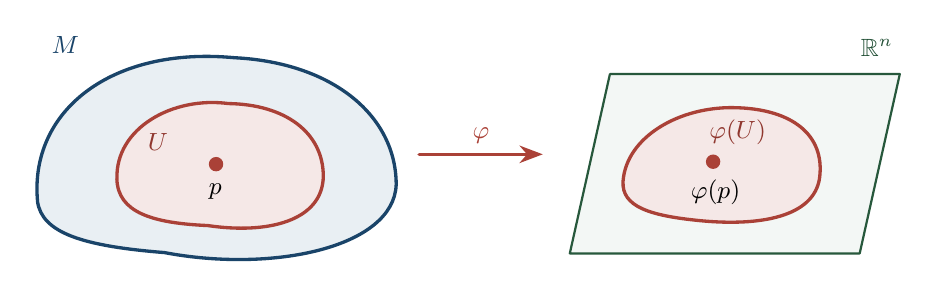
\begin{tikzpicture}[>=Stealth,scale=1.04,line cap=round,line join=round]
% Fragment M oraz wyróżniony otwarty zbiór U.
\filldraw[fill=manifoldblue!10,draw=manifoldblue!75!black,very thick]
 (-5.05,-.55) .. controls (-5.15,.55) and (-4.15,1.34) .. (-2.65,1.2)
 .. controls (-1.43,1.14) and (-.67,.48) .. (-.67,-.35)
 .. controls (-.7,-1.12) and (-2.18,-1.43) .. (-3.5,-1.18)
 .. controls (-4.5,-1.1) and (-5.0,-.94) .. cycle;
\filldraw[fill=manifoldred!12,draw=manifoldred,very thick]
 (-4.08,-.28) .. controls (-4.1,.34) and (-3.4,.73) .. (-2.72,.64)
 .. controls (-2.03,.63) and (-1.56,.29) .. (-1.56,-.25)
 .. controls (-1.57,-.79) and (-2.23,-.96) .. (-2.97,-.85)
 .. controls (-3.65,-.82) and (-4.07,-.69) .. cycle;
\node[manifoldblue!75!black,font=\small\bfseries] at (-4.71,1.35) {$M$};
\node[manifoldred!85!black,font=\small] at (-3.58,.17) {$U$};
\fill[manifoldred] (-2.87,-.1) circle (2.5pt);
\node[font=\small] at (-2.88,-.44) {$p$};
% Obraz mapy w przestrzeni współrzędnych, bez siatki.
\filldraw[fill=manifoldgreen!6,draw=manifoldgreen!70!black,thick]
 (1.45,-1.19)--(4.99,-1.19)--(5.48,1.0)--(1.94,1.0)--cycle;
\filldraw[fill=manifoldred!12,draw=manifoldred,very thick]
 (2.1,-.31) .. controls (2.14,.23) and (2.78,.6) .. (3.45,.59)
 .. controls (4.16,.58) and (4.57,.26) .. (4.5,-.27)
 .. controls (4.43,-.75) and (3.76,-.86) .. (3.04,-.79)
 .. controls (2.43,-.73) and (2.08,-.62) .. cycle;
\node[manifoldgreen!65!black,font=\small\bfseries] at (5.2,1.32) {$\R^n$};
\node[manifoldred!85!black,font=\small] at (3.5,.29) {$\varphi(U)$};
\fill[manifoldred] (3.2,-.07) circle (2.5pt);
\node[font=\small] at (3.23,-.44) {$\varphi(p)$};
\draw[->,very thick,manifoldred] (-.39,.02)--(1.12,.02)
 node[midway,above,font=\small] {$\varphi$};
\end{tikzpicture}
\caption{Mapa $(U,\varphi)$ przenosi otwarty fragment $U\subset M$ na obszar
$\varphi(U)\subset\R^n$; punktowi $p$ przyporządkowuje współrzędne $\varphi(p)$.}
\label{fig:mapa-rozmaitosc}
\end{figure}


\begin{definicja}
Dwie mapy $(U,\varphi)$ i $(V,\psi)$ na $M$ są \emph{zgodne} ($C^\infty$-zgodne), jeżeli
albo $U\cap V=\emptyset$, albo odwzorowania przejścia
\[
\psi\circ\varphi^{-1}\colon\varphi(U\cap V)\to\psi(U\cap V), \qquad
\varphi\circ\psi^{-1}\colon\psi(U\cap V)\to\varphi(U\cap V)
\]
są klasy $C^\infty$ (są to wtedy automatycznie odwzorowania wzajemnie odwrotne między
otwartymi podzbiorami $\R^n$, a więc dyfeomorfizmy).
\end{definicja}



Na Rysunku~\ref{fig:atlas-przejscie-dwie-mapy} pokazano
dwie zgodne mapy i współrzędne punktu
leżącego w ich części wspólnej. Odwzorowanie przejścia
działa \emph{między obrazami tej części wspólnej}, a nie
między całymi $\varphi_\alpha(U_\alpha)$ i
$\varphi_\beta(U_\beta)$, jeśli dziedziny map się różnią.

\begin{figure}[H]
\centering
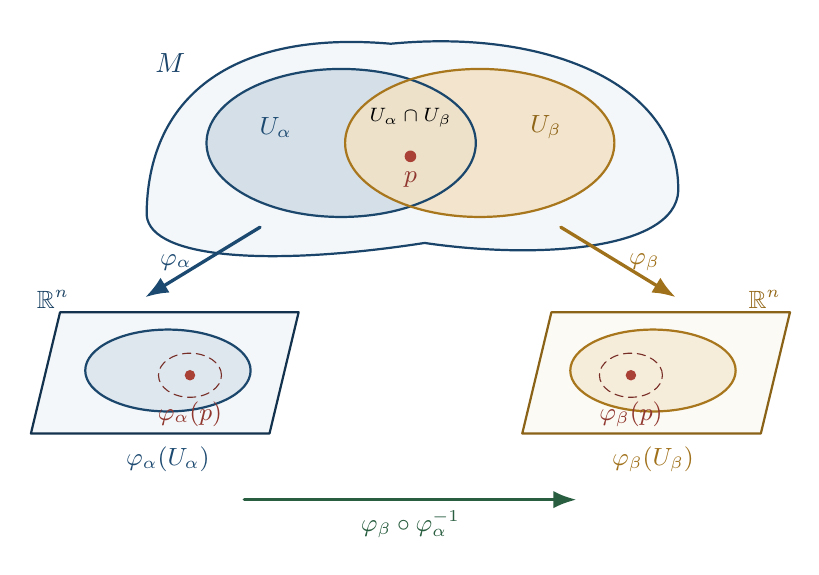
\begin{tikzpicture}[>=Latex,line cap=round,line join=round,
                     font=\small]
  % Fragment rozmaitości i dwa nakładające się obszary map.
  \filldraw[fill=manifoldblue!5,draw=manifoldblue!75!black,thick]
   (-3.35,1.25) .. controls (-3.32,2.76) and (-2.20,3.55)
   .. (-.25,3.38) .. controls (1.72,3.57) and (3.36,2.88)
   .. (3.40,1.59) .. controls (3.48,.77) and (1.68,.63)
   .. (.18,.85) .. controls (-1.90,.53) and (-3.39,.67)
   .. cycle;
  \fill[manifoldblue!22,opacity=.85]
       (-.88,2.12) ellipse (1.71 and .94);
  \fill[manifoldgold!26,opacity=.86]
       (.88,2.12) ellipse (1.71 and .94);
  \draw[manifoldblue!78!black,thick]
       (-.88,2.12) ellipse (1.71 and .94);
  \draw[manifoldgold!82!black,thick]
       (.88,2.12) ellipse (1.71 and .94);
  \node[manifoldblue!75!black,font=\bfseries] at (-3.05,3.13) {$M$};
  \node[manifoldblue!80!black] at (-1.71,2.32) {$U_\alpha$};
  \node[manifoldgold!70!black] at (1.72,2.32) {$U_\beta$};
  \node[font=\scriptsize] at (0,2.44) {$U_\alpha\cap U_\beta$};
  \fill[manifoldred] (0,1.95) circle (2.1pt);
  \node[below,manifoldred!85!black] at (0,1.88) {$p$};
  % Obrazy w dwóch osobnych przestrzeniach współrzędnych.
  \filldraw[fill=manifoldblue!5,draw=manifoldblue!55!black,thick]
       (-4.82,-1.57)--(-1.79,-1.57)--(-1.42,-.03)
       --(-4.45,-.03)--cycle;
  \fill[manifoldblue!15] (-3.08,-.77) ellipse (1.05 and .52);
  \draw[manifoldblue!78!black,thick]
       (-3.08,-.77) ellipse (1.05 and .52);
  \draw[manifoldred!70!black,densely dashed]
       (-2.80,-.83) ellipse (.40 and .28);
  \fill[manifoldred] (-2.80,-.83) circle (1.9pt);
  \node[manifoldred!85!black] at (-2.80,-1.32)
       {$\varphi_\alpha(p)$};
  \node[manifoldblue!70!black] at (-4.54,.13) {$\R^n$};

  \filldraw[fill=manifoldgold!5,draw=manifoldgold!68!black,thick]
       (1.42,-1.57)--(4.45,-1.57)--(4.82,-.03)
       --(1.79,-.03)--cycle;
  \fill[manifoldgold!17] (3.08,-.77) ellipse (1.05 and .52);
  \draw[manifoldgold!82!black,thick]
       (3.08,-.77) ellipse (1.05 and .52);
  \draw[manifoldred!70!black,densely dashed]
       (2.80,-.83) ellipse (.40 and .28);
  \fill[manifoldred] (2.80,-.83) circle (1.9pt);
  \node[manifoldred!85!black] at (2.80,-1.32)
       {$\varphi_\beta(p)$};
  \node[manifoldgold!72!black] at (4.50,.13) {$\R^n$};

  \draw[->,manifoldblue!80!black,very thick]
       (-1.91,1.05)--(-3.37,.16)
       node[midway,left] {$\varphi_\alpha$};
  \draw[->,manifoldgold!78!black,very thick]
       (1.91,1.05)--(3.37,.16)
       node[midway,right] {$\varphi_\beta$};
  \node[manifoldblue!80!black] at (-3.08,-1.90)
       {$\varphi_\alpha(U_\alpha)$};
  \node[manifoldgold!78!black] at (3.08,-1.90)
       {$\varphi_\beta(U_\beta)$};
  \draw[->,manifoldgreen!75!black,very thick]
       (-2.11,-2.41)--(2.11,-2.41)
       node[midway,below] {$\varphi_\beta\circ\varphi_\alpha^{-1}$};
\end{tikzpicture}
\caption{Dwie nakładające się mapy. Przerywane obszary
oznaczają obrazy części wspólnej. Punkt $p$ ma
dwa zapisy współrzędnych, a przejście
$\varphi_\beta\circ\varphi_\alpha^{-1}$ prowadzi
z $\varphi_\alpha(U_\alpha\cap U_\beta)$ do
$\varphi_\beta(U_\alpha\cap U_\beta)$. W atlasie
pozostałe mapy pokrywają ewentualną resztę $M$.}
\label{fig:atlas-przejscie-dwie-mapy}
\end{figure}

\begin{definicja}
\emph{Atlasem} (gładkim, $C^\infty$) na rozmaitości topologicznej $M$ nazywamy rodzinę map
$\mathcal{A}=\{(U_\alpha,\varphi_\alpha)\}_{\alpha\in I}$ taką, że:
\begin{enumerate}[label=(\roman*)]
\item $\bigcup_{\alpha\in I}U_\alpha=M$,
\item mapy $(U_\alpha,\varphi_\alpha)$ oraz $(U_\beta,\varphi_\beta)$ są zgodne dla
wszystkich $\alpha,\beta\in I$.
\end{enumerate}
\end{definicja}



Chcemy teraz porównywać różne atlasy na tej samej przestrzeni topologicznej $M$ — dwa
atlasy powinny wyznaczać tę samą strukturę gładką dokładnie wtedy, gdy razem tworzą
(większy) atlas.

\begin{definicja}
Dwa atlasy $\mathcal{A}_1$, $\mathcal{A}_2$ na $M$ są \emph{równoważne}, $\mathcal A_1\sim
\mathcal A_2$, jeżeli ich suma $\mathcal{A}_1\cup\mathcal{A}_2$ jest atlasem, tzn.\ każda
mapa z $\mathcal{A}_1$ jest zgodna z każdą mapą z $\mathcal{A}_2$.
\end{definicja}

Poniższy lemat techniczny jest kluczowym narzędziem rachunkowym tego paragrafu; wykorzystamy
go dwukrotnie: do dowodu, że $\sim$ jest relacją równoważności, oraz do dowodu istnienia i
jednoznaczności atlasu maksymalnego.

\begin{lemat}\label{lem:zgodnosc-przechodnia}
Niech $(U,\varphi)$, $(W,\eta)$, $(V,\psi)$ będą mapami na $M$ takimi, że $(U,\varphi)$
jest zgodna z $(W,\eta)$, a $(W,\eta)$ jest zgodna z $(V,\psi)$. Wówczas dla dowolnego
punktu $p\in U\cap V\cap W$, odwzorowania $\psi\circ\varphi^{-1}$ i $\varphi\circ\psi^{-1}$
są klasy $C^\infty$ w (odpowiednich) otoczeniach punktów $\varphi(p)$ i $\psi(p)$.
\end{lemat}

\begin{proof}
Na otoczeniu $\varphi(U\cap V\cap W)$ punktu $\varphi(p)$ mamy równość
$\psi\circ\varphi^{-1}=(\psi\circ\eta^{-1})\circ(\eta\circ\varphi^{-1})$; odwzorowanie
$\eta\circ\varphi^{-1}$ jest gładkie na $\varphi(U\cap W)$ (zgodność $(U,\varphi)$ z
$(W,\eta)$), a $\psi\circ\eta^{-1}$ jest gładkie na $\eta(W\cap V)$ (zgodność $(W,\eta)$ z
$(V,\psi)$); złożenie odwzorowań gładkich jest gładkie, więc $\psi\circ\varphi^{-1}$ jest
gładkie w otoczeniu $\varphi(p)$. Analogicznie, na otoczeniu $\psi(p)$:
$\varphi\circ\psi^{-1}=(\varphi\circ\eta^{-1})\circ(\eta\circ\psi^{-1})$ jest złożeniem
odwzorowań gładkich ($\varphi\circ\eta^{-1}$ i $\eta\circ\psi^{-1}$ gładkie, z tych samych
dwóch założeń zgodności), a więc gładkie.
\end{proof}

\begin{stwierdzenie}
Równoważność atlasów jest relacją równoważności na zbiorze wszystkich atlasów na $M$.
\end{stwierdzenie}

\begin{proof}
Zwrotność i symetria są oczywiste z definicji. Sprawdzimy przechodniość. Niech
$\mathcal{A}_1\sim\mathcal{A}_2$ i $\mathcal{A}_2\sim\mathcal{A}_3$; pokażemy, że
$\mathcal{A}_1\sim\mathcal{A}_3$, czyli że dowolna mapa $(U,\varphi)\in\mathcal{A}_1$ jest
zgodna z dowolną mapą $(V,\psi)\in\mathcal{A}_3$. Jeśli $U\cap V=\emptyset$, zgodność jest
trywialna. W przeciwnym razie ustalmy $p\in U\cap V$. Ponieważ $\mathcal{A}_2$ jest atlasem
pokrywającym $M$, istnieje mapa $(W,\eta)\in\mathcal{A}_2$ z $p\in W$. Z założenia
$\mathcal{A}_1\sim\mathcal{A}_2$, mapa $(U,\varphi)$ jest zgodna z $(W,\eta)$; z założenia
$\mathcal{A}_2\sim\mathcal{A}_3$, mapa $(W,\eta)$ jest zgodna z $(V,\psi)$. Na mocy
Lematu~\ref{lem:zgodnosc-przechodnia} (zastosowanego w punkcie $p\in U\cap V\cap W$),
odwzorowania $\psi\circ\varphi^{-1}$ i $\varphi\circ\psi^{-1}$ są gładkie w otoczeniach
odpowiednio $\varphi(p)$ i $\psi(p)$. Ponieważ punkt $p\in U\cap V$ był dowolny, oba te
odwzorowania są gładkie na całych swoich dziedzinach $\varphi(U\cap V)$, $\psi(U\cap V)$
(gładkość jest własnością lokalną). Zatem $(U,\varphi)$ i $(V,\psi)$ są zgodne, co dowodzi
$\mathcal{A}_1\sim\mathcal{A}_3$.
\end{proof}

W praktyce nie chcemy jednak utożsamiać struktury gładkiej z pojedynczym atlasem — dwa
równoważne atlasy powinny wyznaczać \emph{tę samą} strukturę. Wygodnie jest wybrać
kanonicznego reprezentanta każdej klasy równoważności: atlas maksymalny.

\begin{definicja}
Atlas $\mathcal{A}$ na $M$ jest \emph{maksymalny}, jeśli nie jest właściwym podzbiorem
żadnego innego atlasu na $M$, tzn.\ jeśli mapa $(U,\varphi)$ jest zgodna z każdą mapą
należącą do $\mathcal{A}$, to $(U,\varphi)\in\mathcal{A}$.
\end{definicja}

\begin{twierdzenie}\label{tw:atlas-maksymalny}
Każdy atlas $\mathcal{A}$ na $M$ jest zawarty w dokładnie jednym atlasie maksymalnym
$\mathcal{A}^+$, zadanym wzorem
\[
\mathcal{A}^+=\{(U,\varphi)\text{ -- mapa na }M : (U,\varphi)\text{ jest zgodna z każdą
mapą z }\mathcal{A}\}.
\]
Ponadto dwa atlasy $\mathcal{A}_1$, $\mathcal{A}_2$ są równoważne wtedy i tylko wtedy, gdy
$\mathcal{A}_1^+=\mathcal{A}_2^+$.
\end{twierdzenie}

\begin{proof}
\emph{Krok 1: $\mathcal{A}^+$ jest atlasem.} Ponieważ $\mathcal{A}\subseteq\mathcal{A}^+$
(każda mapa z $\mathcal{A}$ jest zgodna z każdą mapą z $\mathcal{A}$, gdyż $\mathcal{A}$
jest atlasem), zbiory dziedzin map z $\mathcal{A}^+$ pokrywają $M$. Pozostaje sprawdzić, że
dowolne dwie mapy $(U,\varphi),(V,\psi)\in\mathcal{A}^+$ są ze sobą zgodne. Ustalmy
$p\in U\cap V$ (dla $U\cap V=\emptyset$ zgodność jest trywialna); ponieważ $\mathcal{A}$
pokrywa $M$, istnieje $(W,\eta)\in\mathcal{A}$ z $p\in W$. Mapa $(U,\varphi)$ jest zgodna z
$(W,\eta)$ (bo $(U,\varphi)\in\mathcal{A}^+$ jest zgodna z każdą mapą z $\mathcal A$), a
$(W,\eta)$ jest zgodna z $(V,\psi)$ (analogicznie, bo $(V,\psi)\in\mathcal A^+$). Na mocy
Lematu~\ref{lem:zgodnosc-przechodnia}, odwzorowania $\psi\circ\varphi^{-1}$,
$\varphi\circ\psi^{-1}$ są gładkie w otoczeniach $\varphi(p)$, $\psi(p)$; wobec dowolności
$p\in U\cap V$, są gładkie na całych dziedzinach $\varphi(U\cap V)$, $\psi(U\cap V)$. Zatem
$\mathcal{A}^+$ jest atlasem.

\emph{Krok 2: $\mathcal{A}^+$ jest maksymalny.} Niech mapa $(U,\varphi)$ będzie zgodna z
każdą mapą należącą do $\mathcal{A}^+$. Ponieważ $\mathcal{A}\subseteq\mathcal{A}^+$, mapa
$(U,\varphi)$ jest w szczególności zgodna z każdą mapą z $\mathcal{A}$, a więc z definicji
$\mathcal{A}^+$ mamy $(U,\varphi)\in\mathcal{A}^+$.

\emph{Krok 3: jednoznaczność.} Niech $\mathcal B\supseteq\mathcal A$ będzie atlasem
maksymalnym. Ponieważ $\mathcal B$ jest atlasem i $\mathcal A\subseteq\mathcal B$, każda
mapa z $\mathcal B$ jest zgodna z każdą mapą z $\mathcal A$ (obie należą do atlasu
$\mathcal B$) — więc $\mathcal B\subseteq\mathcal A^+$ z definicji $\mathcal A^+$.

Odwrotnie, niech $(U,\varphi)\in\mathcal A^+$; pokażemy $(U,\varphi)\in\mathcal B$, co —
wobec dowolności $(U,\varphi)\in\mathcal A^+$ — da $\mathcal A^+\subseteq\mathcal B$, a
wraz z poprzednią inkluzją: $\mathcal B=\mathcal A^+$. Z maksymalności $\mathcal B$
wystarczy pokazać, że $(U,\varphi)$ jest zgodna z każdą mapą $(V,\psi)\in\mathcal B$.
Ustalmy taką mapę i punkt $p\in U\cap V$ (dla $U\cap V=\emptyset$ zgodność jest trywialna).
Ponieważ $\mathcal A$ pokrywa $M$, istnieje $(W,\eta)\in\mathcal A$ z $p\in W$. Mapa
$(U,\varphi)$ jest zgodna z $(W,\eta)$ (bo $(U,\varphi)\in\mathcal A^+$), a $(W,\eta)\in
\mathcal A\subseteq\mathcal B$ jest zgodna z $(V,\psi)\in\mathcal B$ (bo obie należą do
atlasu $\mathcal B$). Na mocy Lematu~\ref{lem:zgodnosc-przechodnia}, $(U,\varphi)$ i
$(V,\psi)$ są zgodne w otoczeniu $p$; wobec dowolności $p\in U\cap V$ — zgodne na całych
dziedzinach. Zatem $(U,\varphi)$ jest zgodna z każdą mapą z $\mathcal B$, więc — z
maksymalności $\mathcal B$ — $(U,\varphi)\in\mathcal B$.

\emph{Krok 4: $\mathcal A_1\sim\mathcal A_2\iff\mathcal A_1^+=\mathcal A_2^+$.}
($\Leftarrow$) Jeśli $\mathcal A_1^+=\mathcal A_2^+=:\mathcal B$, to $\mathcal A_1\subseteq
\mathcal B$ i $\mathcal A_2\subseteq\mathcal B$, a skoro $\mathcal B$ jest atlasem, każda
mapa z $\mathcal A_1$ jest zgodna z każdą mapą z $\mathcal B$, w szczególności z każdą mapą
z $\mathcal A_2$ — czyli $\mathcal A_1\sim\mathcal A_2$.

($\Rightarrow$) Załóżmy $\mathcal A_1\sim\mathcal A_2$. Pokażemy $\mathcal A_1^+\subseteq
\mathcal A_2^+$ (inkluzja odwrotna analogicznie, skąd równość). Niech $(U,\varphi)\in
\mathcal A_1^+$. Ustalmy dowolną mapę $(V,\psi)\in\mathcal A_2$ i (dla $U\cap V\neq
\emptyset$, inaczej trywialnie) punkt $p\in U\cap V$. Ponieważ $\mathcal A_1$ pokrywa $M$,
istnieje $(W,\eta)\in\mathcal A_1$ z $p\in W$. Mapa $(U,\varphi)$ jest zgodna z $(W,\eta)\in
\mathcal A_1$ (bo $(U,\varphi)\in\mathcal A_1^+$), a $(W,\eta)\in\mathcal A_1$ jest zgodna z
$(V,\psi)\in\mathcal A_2$ (bo $\mathcal A_1\sim\mathcal A_2$). Na mocy
Lematu~\ref{lem:zgodnosc-przechodnia}, $(U,\varphi)$ i $(V,\psi)$ są zgodne w otoczeniu
$p$; wobec dowolności $p\in U\cap V$ — na całych dziedzinach. Zatem $(U,\varphi)$ jest
zgodna z $(V,\psi)$; wobec dowolności $(V,\psi)\in\mathcal A_2$, mamy $(U,\varphi)\in
\mathcal A_2^+$.
\end{proof}

Powyższe twierdzenie pozwala oddzielić topologię przestrzeni od
wyboru współrzędnych, w których będziemy różniczkować.

\begin{definicja}[Struktura różniczkowa]\label{def:struktura-rozniczkowa}
\index{struktura rozniczkowa@Struktura różniczkowa}
\emph{Strukturą różniczkową} klasy $C^\infty$ na rozmaitości
topologicznej $M$ nazywamy klasę równoważności atlasów gładkich
na $M$. Równoważnie, na mocy Twierdzenia~\ref{tw:atlas-maksymalny},
jest nią jedyny atlas maksymalny $\mathcal A=\mathcal A_0^+$
zawierający dowolny atlas $\mathcal A_0$ z tej klasy. Mapy
należące do $\mathcal A$ nazywamy \emph{dopuszczalnymi}.
\end{definicja}

\begin{definicja}[Rozmaitość gładka]\label{def:rozmaitosc-gladka}
\index{rozmaitosc gladka@Rozmaitość gładka}
\emph{Rozmaitością gładką} (klasy $C^\infty$) wymiaru $n$
nazywamy parę $(M,\mathcal A)$, gdzie $M$ jest rozmaitością
topologiczną wymiaru $n$, a $\mathcal A$ jest strukturą
różniczkową zapisaną jako atlas maksymalny.
\end{definicja}

W praktyce wystarczy podać mały atlas $\mathcal A_0$:
wyznacza on jednoznacznie strukturę $\mathcal A_0^+$.
Topologia określa, które mapy współrzędnych są homeomorfizmami;
struktura różniczkowa określa dodatkowo, które przejścia
między nimi są gładkie.

\begin{przyklad}[Różne struktury na tej samej przestrzeni]
Na topologicznej prostej $\R$ atlas $\mathcal A_{\mathrm{std}}$
z mapą $\id\colon\R\to\R$ i atlas $\mathcal A_h$ z mapą
$h\colon\R\to\R$, $h(x)=x^3$, są osobno atlasami gładkimi.
Nie są równoważne: w jednym kierunku
przejście jest dane przez $h^{-1}(u)=\sqrt[3]{u}$,
które nie jest różniczkowalne w zerze.
Definiują zatem różne struktury na \emph{ustalonym} zbiorze
topologicznym $\R$, choć otrzymane rozmaitości są
dyfeomorficzne (w sensie definicji~\ref{def dyfeo}): dyfeomorfizm
$h\colon(\R,\mathcal A_h^+)\to(\R,\mathcal A_{\mathrm{std}}^+)$
ma w odpowiednich mapach współrzędnych postać identyczności.
\end{przyklad}

\begin{uwaga}[Intuicja: mapa, atlas i rozmaitość]
Najprostszym sposobem zrozumienia pojęć \emph{mapy}, \emph{atlasu} i
\emph{rozmaitości} jest analogia z powierzchnią Ziemi.

Powierzchnia Ziemi jest obiektem zakrzywionym i nie możemy przedstawić jej
w całości na jednej płaskiej kartce bez zniekształceń. Możemy jednak wybrać
niewielki fragment powierzchni, na przykład okolice Krakowa, i przedstawić go
na płaskiej mapie. Matematycznie dokładnie taką rolę pełni \emph{mapa}
rozmaitości.

Jeżeli $M$ jest rozmaitością, to mapa jest parą $(U,\varphi)$, gdzie
$U\subset M$ jest otwartym fragmentem rozmaitości, a $\varphi\colon U\longrightarrow \varphi(U)\subset\mathbb{R}^n$
jest homeomorfizmem. Oznacza to, że punkty znajdujące się w $U$ możemy opisać
za pomocą zwykłych współrzędnych $(x^1,\ldots,x^n)\in\mathbb{R}^n$.
Można więc myśleć o $\varphi$ jako o sposobie ``rozłożenia'' niewielkiego
fragmentu rozmaitości na płaskiej przestrzeni $\mathbb{R}^n$.

Jedna mapa zazwyczaj nie wystarcza do opisania całej przestrzeni. Podobnie
jedna mapa geograficzna przedstawiająca okolice Krakowa nie opisuje całej
powierzchni Ziemi. Potrzebujemy wielu map $(U_\alpha,\varphi_\alpha)$,
których dziedziny pokrywają całą przestrzeń:
\[
    M=\bigcup_{\alpha}U_\alpha.
\]
Taki zbiór map nazywamy \emph{atlasem}.

Jeżeli dwa obszary $U_\alpha$ i $U_\beta$ nachodzą na siebie, to ten sam punkt
rozmaitości może mieć dwa różne opisy współrzędnościowe. Przejście pomiędzy
nimi opisuje odwzorowanie $\varphi_\beta\circ\varphi_\alpha^{-1}$,
zwane odwzorowaniem przejścia. Można je porównać do przeliczania współrzędnych
tego samego miejsca pomiędzy dwiema zachodzącymi na siebie mapami
geograficznymi.

\emph{Rozmaitość} jest zatem przestrzenią, która globalnie może być
skomplikowana lub zakrzywiona, ale w dostatecznie małym otoczeniu każdego
punktu wygląda jak zwykła przestrzeń euklidesowa $\mathbb{R}^n$.

W skrócie:
\[
\boxed{
\begin{array}{ccl}
\text{mapa}      &\longleftrightarrow& \text{lokalny układ współrzędnych},\\[2mm]
\text{atlas}     &\longleftrightarrow& \text{zbiór map opisujących całą przestrzeń},\\[2mm]
\text{rozmaitość}&\longleftrightarrow& \text{przestrzeń lokalnie wyglądająca jak }\mathbb{R}^n.
\end{array}}
\]

Przykładowo sfera $S^2$ nie jest płaską częścią $\mathbb{R}^2$, ale każdy jej
dostatecznie mały fragment można opisać za pomocą dwóch współrzędnych.
Dlatego $S^2$ jest dwuwymiarową rozmaitością.
\end{uwaga}

Od tej pory, mówiąc o rozmaitości $M$, będziemy mieli na myśli rozmaitość gładką — parę
$(M,\mathcal{A})$ — pomijając $\mathcal{A}$ w oznaczeniach, gdy nie prowadzi to do
nieporozumień.

\section{Rozmaitości z brzegiem}
\label{sec:rozmaitosci-z-brzegiem-1}
\index{brzeg rozmaitosci@Brzeg rozmaitości}

Wnętrze dysku wygląda lokalnie jak otwarty zbiór w $\R^n$,
ale punkt na jego brzegu ma tylko jedną stronę. Modelem takiego
otoczenia jest półprzestrzeń $\mathbb H^n=\{(x^1,\ldots,x^n)\in\R^n:x^n\geq0\}, \ n\geq1$.
Otwartość podzbioru $\mathbb H^n$ rozumiemy w topologii względnej.

\begin{definicja}[Rozmaitość gładka z brzegiem]
\index{rozmaitosc gladka z brzegiem@Rozmaitość gładka z brzegiem}
\label{def:rozmaitosc-z-brzegiem-1}
\emph{Rozmaitość gładka z brzegiem} wymiaru $n\geq1$ to przestrzeń
Hausdorffa spełniająca drugi aksjomat przeliczalności, wyposażona
w atlas homeomorfizmów
$\varphi_\alpha:U_\alpha\to V_\alpha$ na zbiory
$V_\alpha$ otwarte w $\mathbb H^n$. Na częściach wspólnych
odwzorowania przejścia i ich odwrotności mają być gładkie:
w otoczeniu każdego punktu rozumie się przez to istnienie
gładkiego przedłużenia na otwarty zbiór w $\R^n$.
Maksymalny atlas zgodny z tym atlasem wyznacza strukturę gładką,
tak jak w Twierdzeniu~\ref{tw:atlas-maksymalny}.
\emph{Brzegiem rozmaitości} nazywamy zbiór
\[
 \partial M=\{p\in M:\varphi_\alpha(p)^n=0
             \text{ w pewnej mapie }(U_\alpha,\varphi_\alpha)\}.
\]
Pozostałe punkty tworzą wnętrze $M^\circ=M\setminus\partial M$.
Dla wymiaru $0$ przyjmujemy $\partial M=\varnothing$.
\end{definicja}

Warunek „w pewnej mapie” jest poprawny dzięki następującemu
faktowi; jednocześnie pokazuje, że brzeg nie zależy od wyboru
współrzędnych.

\begin{stwierdzenie}[Niezależność brzegu od mapy]
\label{prop:brzeg-niezalezny-1}
Dla $n\geq1$, jeśli $p$ ma ostatnią współrzędną równą $0$ w jednej
mapie półprzestrzennej, to ma ją równą $0$ w każdej
mapie półprzestrzennej, której dziedzina zawiera $p$.
Zbiór $\partial M$ jest zamknięty w $M$ i z map ograniczonych
do $\partial M$ otrzymuje strukturę gładkiej
rozmaitości wymiaru $n-1$ bez brzegu.
\end{stwierdzenie}
\begin{proof}
Przypuśćmy, że $\varphi(p)$ leży na płaszczyźnie
$x^n=0$, a $\psi(p)$ jest punktem wnętrza $\mathbb H^n$.
Ograniczmy mapy do wspólnego dostatecznie małego otoczenia
$p$. Wtedy $\psi$ odwzorowuje je na zbiór otwarty w $\R^n$,
a $\varphi\circ\psi^{-1}$ jest ciągłą injekcją tego zbioru
do $\R^n$. Twierdzenie Brouwera o niezmienniczości obszaru
orzeka, że obraz takiej injekcji jest otwarty w $\R^n$.
Obraz leży jednak w $\mathbb H^n$ i zawiera punkt
$\varphi(p)$ na jego płaszczyźnie brzegowej, więc nie może
być otwarty w $\R^n$. Sprzeczność dowodzi pierwszej tezy.
Dokładne sformułowanie użytego wyniku zewnętrznego podaje
\href{https://pi.math.cornell.edu/~hatcher/AT/AT.pdf}
{A. Hatcher, \emph{Algebraic Topology}, twierdzenie 2B.3}.

W każdej mapie punkty z $x^n>0$ tworzą zbiór otwarty.
Zatem $M^\circ$ jest otwarty, a $\partial M$ zamknięty.
Ograniczenie mapy $\varphi$ do
$U\cap\partial M$ przyjmuje wartości w otwartym
podzbiorze $\R^{n-1}\times\{0\}$. Przejścia między
tymi ograniczeniami są gładkie, bo są ograniczeniami
gładkich przedłużeń przejść na $\R^n$; to samo dotyczy
odwrotności. Są to więc mapy gładkiej rozmaitości
wymiaru $n-1$. Każda z nich ma obraz otwarty w całej
$\R^{n-1}$, czyli $\partial M$ nie ma własnego brzegu.
\end{proof}

W punkcie brzegu definiujemy $T_pM$ przez
wektory współrzędnych w półprzestrzennej mapie,
równoważnie przez derywacje gładkich kiełków
funkcji w $p$. Pełną konstrukcję i niezależność od przedłużeń
podamy po wprowadzeniu przestrzeni stycznej, w
Stwierdzeniu~\ref{prop:styczna-brzeg-1}. Ten model ma $n$ niezależnych
kierunków: $T_pM\cong\R^n$, natomiast
$T_p\partial M\cong\{v\in\R^n:v^n=0\}$ ma wymiar $n-1$.
Wektor o ujemnej ostatniej współrzędnej należy do $T_pM$,
choć nie jest prędkością krzywej biegnącej od $p$ do wnętrza
przy dodatnim czasie. Przykładowo $T_0[0,1]\cong\R$,
podczas gdy $T_0\partial[0,1]=0$.
Model przez krzywe określone na otwartym przedziale,
omówiony w Sekcji~\ref{sec:przestrzen-styczna},
dotyczy punktów wnętrza: w punkcie brzegu
dwustronna krzywa w $M$ nie reprezentuje
kierunku poprzecznego do brzegu.

\begin{przyklad}[Kula, okrąg i brzeg otaczającej przestrzeni]
\label{prz:brzeg-kula-okrag-1}
Domknięta kula $D^n=\{x\in\R^n:|x|\leq1\}$ ma brzeg
rozmaitościowy $S^{n-1}$. Rzeczywiście, przy $|p|=1$
funkcja $\rho(x)=1-|x|^2$ ma niezerową różniczkę
$\dd\rho_p(v)=-2\langle p,v\rangle$. Twierdzenie o funkcji
odwrotnej pozwala użyć $\rho$ jako ostatniej lokalnej
współrzędnej, zatem $D^n$ odpowiada warunkowi $\rho\geq0$.
Z kolei brzeg okręgu $S^1\subset\R^2$ jako rozmaitości
(w sensie Definicji~\ref{def:rozmaitosc-z-brzegiem-1})
jest pusty: $\partial S^1=\varnothing$. Jego brzeg topologiczny
jako \emph{podzbioru $\R^2$} jest natomiast całym $S^1$: okrąg ma
puste wnętrze w $\R^2$ i jest domknięty.
Te dwa znaczenia słowa „brzeg” trzeba odróżniać.
\end{przyklad}

Produkt dwóch rozmaitości z brzegiem może mieć
\emph{naroża}. W kwadracie $[0,1]^2$ przy wierzchołku
naturalny model pochodzący z zanurzenia to
$[0,\infty)^2$, z dwiema ścianami brzegowymi.
W rachunku uchwytów spotkamy taki model na
$\partial D^k\times\partial D^{n-k}$; naroże można
zaokrąglić w małym otoczeniu, zachowując części
odległe od niego. To operacja na gładkiej geometrii
brzegu, a nie zmiana tego, które punkty są brzegowe
topologicznie. Kołnierze i takie zaokrąglanie pojawią się
w Sekcji~\ref{sec:kolnierz-15} i przy uchwytach w
Sekcji~\ref{sec:uchwyt-morse-17}.

\section{Rozmaitości zespolone}

Analogicznie do konstrukcji z poprzedniego paragrafu, możemy modelować rozmaitość lokalnie
nie na $\R^n$, lecz na $\C^n$, żądając przy tym, by odwzorowania przejścia między mapami
były holomorficzne, a nie tylko gładkie.

\begin{definicja}
\emph{Rozmaitością zespoloną} wymiaru (zespolonego) $n$ nazywamy przestrzeń Hausdorffa $M$
spełniającą drugi aksjomat przeliczalności, wyposażoną w atlas $\{(U_\alpha,\varphi_\alpha)\}$
map $\varphi_\alpha\colon U_\alpha\to\varphi_\alpha(U_\alpha)\subseteq\C^n$ (homeomorfizmów
na zbiory otwarte w $\C^n\cong\R^{2n}$), takich że odwzorowania przejścia
\[
\varphi_\beta\circ\varphi_\alpha^{-1}\colon\varphi_\alpha(U_\alpha\cap U_\beta)\to
\varphi_\beta(U_\alpha\cap U_\beta)
\]
są \emph{holomorficzne} (jako odwzorowania między otwartymi podzbiorami $\C^n$), wraz z
maksymalnym takim atlasem (konstrukcja atlasu maksymalnego przebiega dosłownie tak samo,
jak w Sekcji~\ref{sec:atlas}, z ,,gładki'' zastąpionym przez ,,holomorficzny'' — złożenie odwzorowań
holomorficznych jest holomorficzne, więc Lemat~\ref{lem:zgodnosc-przechodnia} i
Twierdzenie~\ref{tw:atlas-maksymalny} przenoszą się bez zmian).
\end{definicja}

\begin{uwaga}
Utożsamiając $\C^n\cong\R^{2n}$ (przez część rzeczywistą i urojoną każdej współrzędnej)
oraz przypominając, że każde odwzorowanie holomorficzne jest w szczególności odwzorowaniem
gładkim (klasy $C^\infty$) w sensie rzeczywistym (ze wzoru całkowego
Cauchy'ego na małym polidysku wynika lokalne rozwinięcie w szereg potęgowy,
który można różniczkować wyraz po wyrazie), widzimy, że \emph{każda rozmaitość zespolona
wymiaru $n$ jest w naturalny sposób rzeczywistą rozmaitością gładką wymiaru $2n$}. Implikacja
odwrotna jest fałszywa: nie każda parzystowymiarowa rozmaitość gładka dopuszcza strukturę
zespoloną (a nawet jeśli dopuszcza, struktura taka zwykle nie jest jednoznaczna).
\end{uwaga}

\begin{przyklad}[Zespolona przestrzeń rzutowa]
Niech $\C_*:=\C\setminus\{0\}$ oznacza zbiór niezerowych
liczb zespolonych.
Zespolonym odpowiednikiem $\mathbb{RP}^n$ z
Przykładu~\ref{prz:RPn} jest przestrzeń ilorazowa $\mathbb{CP}^n := (\C^{n+1}\setminus\{0\})/\!\sim$,
gdzie
\[
z\sim w
\iff
\exists\,\lambda\in\C_*
\quad\text{takie, że}\quad
z=\lambda w.
\]
Przestrzeń $\mathbb{CP}^n$ wyposażamy w topologię ilorazową.
Punkty zapisujemy w postaci $[z^0:z^1:\dots:z^n]$,
przy czym
\[
[z^0:\dots:z^n]
=
[\lambda z^0:\dots:\lambda z^n]
\qquad
\text{dla każdego }\lambda\in\C_*.
\]

Dla $i=0,\dots,n$ definiujemy $U_i = \{[z^0:\dots:z^n]\in\mathbb{CP}^n:z^i\neq0\}$.
Zbiory $U_i$ są otwarte i pokrywają całą przestrzeń $\mathbb{CP}^n$.
Na każdym z nich definiujemy mapę $\varphi_i:U_i\longrightarrow\C^n$
wzorem
\[
\varphi_i([z^0:\dots:z^n])
=
\left(
\frac{z^0}{z^i},
\dots,
\frac{z^{i-1}}{z^i},
\frac{z^{i+1}}{z^i},
\dots,
\frac{z^n}{z^i}
\right).
\]
Jej odwrotność jest dana jawnie przez
\[
\varphi_i^{-1}
(w^0,\dots,w^{i-1},w^{i+1},\dots,w^n)
=
[w^0:\dots:w^{i-1}:1:w^{i+1}:\dots:w^n].
\]
Sprawdźmy także ciągłość, której nie daje sama bijektywność.
Niech $\pi\colon\C^{n+1}\setminus\{0\}\to\mathbb{CP}^n$ będzie
rzutowaniem ilorazowym. Przeciwobraz $\pi^{-1}(U_i)=\{z:z^i\ne0\}$
jest otwarty, zatem $U_i$ jest otwarty. Ograniczenie
$\pi\colon\pi^{-1}(U_i)\to U_i$ także jest odwzorowaniem ilorazowym:
otwarty w $\pi^{-1}(U_i)$ przeciwobraz podzbioru $U_i$ jest otwarty
w całej dziedzinie $\pi$, więc sam podzbiór jest otwarty w ilorazie.
Składowe $\varphi_i\circ\pi$ są ciągłymi ilorazami współrzędnych;
z własności topologii ilorazowej wynika ciągłość $\varphi_i$.
Podany wzór na $\varphi_i^{-1}$ jest złożeniem ciągłego wstawienia
współrzędnej $1$ z $\pi$. Każda $\varphi_i$ jest więc homeomorfizmem
pomiędzy $U_i$ a $\C^n$.

Na przecięciu $U_i\cap U_j$ ten sam punkt przestrzeni
$\mathbb{CP}^n$ posiada dwa różne opisy współrzędnościowe.
Przejście pomiędzy nimi jest opisane przez odwzorowanie $\varphi_j\circ\varphi_i^{-1}$.
Jego składowe są ilorazami wielomianów zespolonych, przy czym
mianowniki nie znikają na dziedzinie odwzorowania. Odwzorowania
przejścia są zatem holomorficzne. Aksjomat Hausdorffa i istnienie
przeliczalnej bazy topologii sprawdzimy w dowodzie
twierdzenia~\ref{thm:rzutowe-zwarte-1}. Łącznie daje to strukturę
rozmaitości zespolonej wymiaru $n$ na $\mathbb{CP}^n$, a więc również
rzeczywistej rozmaitości gładkiej wymiaru $2n$.

Rozważmy teraz szczególny przypadek $n=1$. Otrzymujemy
\emph{sferę Riemanna} $\mathbb{CP}^1$.
Mamy wówczas dwa zbiory $U_0=\{[z^0:z^1]:z^0\neq0\}, \ U_1=\{[z^0:z^1]:z^1\neq0\}$,
oraz mapy
\[
\varphi_0:U_0\longrightarrow\C,
\qquad
\varphi_0([z^0:z^1])=\frac{z^1}{z^0},
\]
i
\[
\varphi_1:U_1\longrightarrow\C,
\qquad
\varphi_1([z^0:z^1])=\frac{z^0}{z^1}.
\]
Każda z tych map identyfikuje odpowiedni fragment
$\mathbb{CP}^1$ z kopią płaszczyzny zespolonej $\C$.

Na przecięciu $U_0\cap U_1 = \{[z^0:z^1]:z^0\neq0,\ z^1\neq0\}$
ten sam punkt ma w pierwszej mapie współrzędną $w = \varphi_0([z^0:z^1]) = \frac{z^1}{z^0}$,
natomiast w drugiej mapie współrzędną $v = \varphi_1([z^0:z^1]) = \frac{z^0}{z^1}$.
Stąd $v=\frac1w$.
Odwzorowanie przejścia ma więc postać $\varphi_1\circ\varphi_0^{-1}(w) = \frac1w, \ w\in\C_*$.

Możemy zatem patrzeć na $\mathbb{CP}^1$ jako na przestrzeń otrzymaną
z dwóch rozłącznych kopii płaszczyzny zespolonej, $\C_0\sqcup\C_1$,
przez utożsamienie punktów należących do ich niezerowych części zgodnie
z regułą $w\in\C_0\setminus\{0\} \quad\sim\quad \frac1w\in\C_1\setminus\{0\}$.
W tym właśnie sensie mówi się, że dwie kopie $\C$ są
\emph{sklejone za pomocą odwzorowania przejścia} $w\longmapsto\frac1w$.
Nie sklejamy więc całych płaszczyzn punkt po punkcie, lecz utożsamiamy
jedynie te punkty obu kopii $\C$, które odpowiadają temu samemu punktowi
przestrzeni $\mathbb{CP}^1$ na części wspólnej $U_0\cap U_1$.

Punkt $0\in\C_0$ odpowiada punktowi $[1:0]\in\mathbb{CP}^1$,
natomiast punkt $0\in\C_1$ odpowiada punktowi $[0:1]\in\mathbb{CP}^1$.
W szczególności, patrząc wyłącznie przez mapę $\varphi_0$, punkt
$[0:1]$ można interpretować jako dodatkowy punkt w nieskończoności.
Dlatego często zapisuje się $\mathbb{CP}^1 \cong \C\cup\{\infty\}$.

Przestrzeń $\mathbb{CP}^1$ jest dyfeomorficzna ze sferą $S^2$.
Trzeba jednak uważać na wybór zespolonych współrzędnych
stereograficznych. Zwykłe rzeczywiste rzuty stereograficzne z
Przykładu~\ref{prz:sfera}, po utożsamieniu $\R^2=\C$, prowadzą do
odwzorowania przejścia $w\longmapsto\frac{w}{|w|^2} = \frac1{\overline{w}}$,
które nie jest holomorficzne.

Aby otrzymać strukturę zespoloną zgodną ze strukturą na
$\mathbb{CP}^1$, wybieramy na $S^2$ współrzędne
\[
\zeta_N(x)
=
\frac{x^1+ix^2}{1-x^3},
\qquad
\zeta_S(x)
=
\frac{x^1-ix^2}{1+x^3}.
\]
Wtedy na części wspólnej zachodzi $\zeta_S\circ\zeta_N^{-1}(w) = \frac1w$.

Jawny dyfeomorfizm $H:\mathbb{CP}^1\longrightarrow S^2$
jest dany wzorem
\[
H([z^0:z^1])
=
\frac{
\big(
2\Re(\overline{z^0}z^1),
2\Im(\overline{z^0}z^1),
|z^1|^2-|z^0|^2
\big)
}{
|z^0|^2+|z^1|^2
}.
\]
Skalowanie obu współrzędnych przez $\lambda\neq0$ mnoży licznik
i mianownik przez $|\lambda|^2$, dlatego wzór jest dobrze określony
na klasach równoważności.

Ponadto
\[
4|z^0|^2|z^1|^2
+
\big(|z^1|^2-|z^0|^2\big)^2
=
\big(|z^0|^2+|z^1|^2\big)^2,
\]
co pokazuje, że obraz odwzorowania $H$ leży na sferze $S^2$.

W wybranych współrzędnych mamy $\zeta_N\circ H=\varphi_0, \ \zeta_S\circ H=\varphi_1$.
Pierwsza z tych równości daje bijekcję $U_0\longrightarrow S^2\setminus\{N\}$,
natomiast pozostały punkt $[0:1]$
przechodzi na biegun północny $N$.
W lokalnych współrzędnych odwzorowanie $H$ oraz jego odwrotność są
tożsamościami, co pokazuje, że $\mathbb{CP}^1\cong S^2$
jako rozmaitości gładkie.
\end{przyklad}


\begin{figure}[h]
\centering
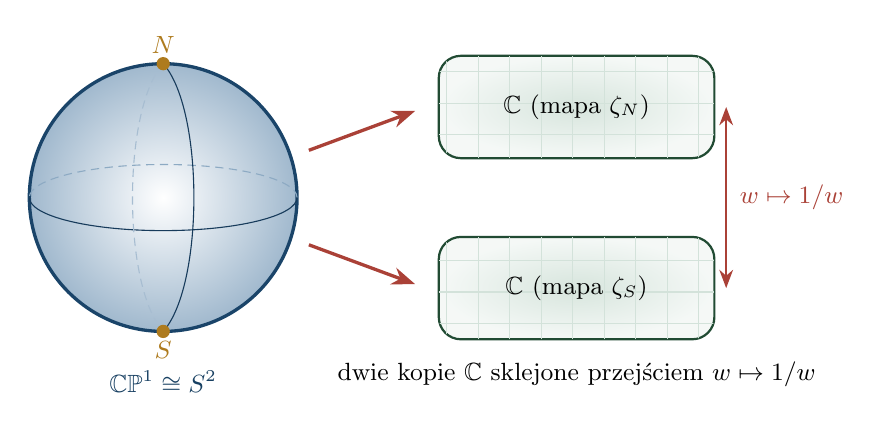
\begin{tikzpicture}[>=Stealth,scale=1]
% Sfera: jasna plama i podział równika na część widoczną oraz ukrytą.
\shade[inner color=white,outer color=manifoldblue!43] (0,0) circle (1.7);
\draw[manifoldblue!75!black,very thick] (0,0) circle (1.7);
\draw[manifoldblue!52,densely dashed,thin]
  (1.7,0) arc[start angle=0,end angle=180,x radius=1.7,y radius=.42];
\draw[manifoldblue!65!black,thin]
  (-1.7,0) arc[start angle=180,end angle=360,x radius=1.7,y radius=.42];
\draw[manifoldblue!40,densely dashed,thin] (0,1.7)
  .. controls (-.52,1.12) and (-.52,-1.12) .. (0,-1.7);
\draw[manifoldblue!65!black,thin] (0,1.7)
  .. controls (.52,1.12) and (.52,-1.12) .. (0,-1.7);
% bieguny
\fill[manifoldgold!85!black] (0,1.7) circle (2.4pt) node[above,font=\small]{$N$};
\fill[manifoldgold!85!black] (0,-1.7) circle (2.4pt) node[below,font=\small]{$S$};
\node[manifoldblue!70!black,font=\small] at (0,-2.35) {$\mathbb{CP}^1\cong S^2$};
% --- strzałki do płaszczyzn C ---
\draw[->,very thick,manifoldred] (1.85,0.6) -- (3.2,1.1);
\draw[->,very thick,manifoldred] (1.85,-0.6) -- (3.2,-1.1);
% --- dwie kopie C (zaokrąglone) ---
% górna
\shade[inner color=manifoldgreen!20, outer color=manifoldgreen!5, rounded corners=8pt]
  (3.5,0.5) rectangle (7.0,1.8);
\draw[manifoldgreen!60!black,thick,rounded corners=8pt]
  (3.5,0.5) rectangle (7.0,1.8);
\begin{scope}
  \clip[rounded corners=8pt] (3.5,0.5) rectangle (7.0,1.8);
  \draw[step=0.4,manifoldgreen!22,thin] (3.5,0.5) grid (7.0,1.8);
\end{scope}
\node[font=\small] at (5.25,1.15) {$\C$ (mapa $\zeta_N$)};
% dolna
\shade[inner color=manifoldgreen!20, outer color=manifoldgreen!5, rounded corners=8pt]
  (3.5,-1.8) rectangle (7.0,-0.5);
\draw[manifoldgreen!60!black,thick,rounded corners=8pt]
  (3.5,-1.8) rectangle (7.0,-0.5);
\begin{scope}
  \clip[rounded corners=8pt] (3.5,-1.8) rectangle (7.0,-0.5);
  \draw[step=0.4,manifoldgreen!22,thin] (3.5,-1.8) grid (7.0,-0.5);
\end{scope}
\node[font=\small] at (5.25,-1.15) {$\C$ (mapa $\zeta_S$)};
% przejście w↦1/w
\draw[<->,thick,manifoldred] (7.15,1.15) -- (7.15,-1.15);
\node[manifoldred,font=\small,right] at (7.2,0) {$w\mapsto 1/w$};
\node[font=\small] at (5.25,-2.25) {dwie kopie $\C$ sklejone przejściem $w\mapsto 1/w$};
\end{tikzpicture}
\caption{Schematyczna interpretacja $\mathbb{CP}^1$ jako sfery Riemanna:
dwie mapy zespolone pokrywają sferę; w mapie południowej odwrócono
znak drugiej współrzędnej rzeczywistej. Przejście $1/w$ jest określone dla $w\ne0$.}
\label{fig:cp1}
\end{figure}

\section{Odwzorowania gładkie między rozmaitościami}

\begin{definicja}
Niech $M$, $N$ będą rozmaitościami gładkimi wymiarów odpowiednio $m$, $n$. Odwzorowanie
$F\colon M\to N$ jest \emph{gładkie} (klasy $C^\infty$) w punkcie $p\in M$, jeżeli dla
pewnej (równoważnie: każdej) mapy dopuszczalnej $(U,\varphi)$ wokół $p$ i mapy
dopuszczalnej $(V,\psi)$ wokół $F(p)$ z $F(U)\subseteq V$, odwzorowanie
$\psi\circ F\circ\varphi^{-1}\colon\varphi(U)\to\psi(V)$
jest gładkie (klasy $C^\infty$) w pewnym otwartym otoczeniu
$\varphi(p)$. Odwzorowanie $F$ jest gładkie, jeśli jest gładkie w każdym punkcie $p\in M$.
Zbiór wszystkich gładkich funkcji $M\to\R$ oznaczamy $C^\infty(M)$.
\end{definicja}
\begin{figure}[ht]
\centering
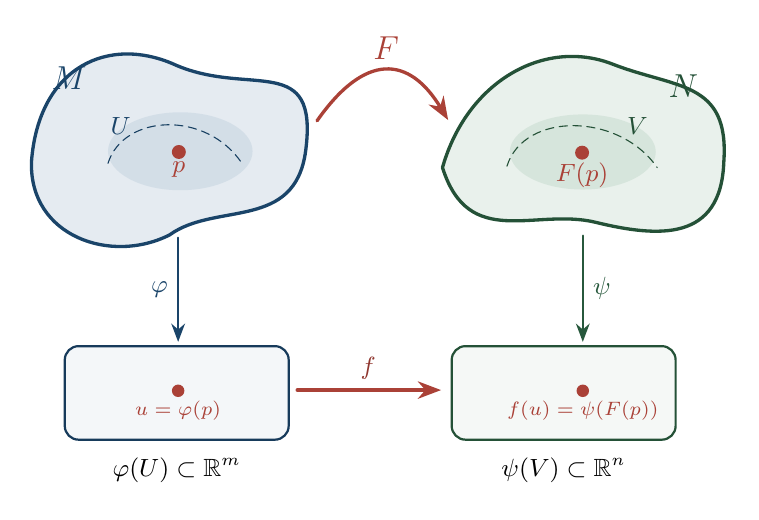
\begin{tikzpicture}[>=Stealth,scale=.9,line cap=round,line join=round]
% Dwie pofalowane powierzchnie z siatką lokalnych współrzędnych.
\def\Mshape{(-4.75,.2) .. controls (-4.65,1.55) and (-3.65,2.0) .. (-2.7,1.56)
 .. controls (-1.65,1.12) and (-.7,1.75) .. (-.88,.36)
 .. controls (-1.03,-.78) and (-2.15,-.36) .. (-2.8,-.83)
 .. controls (-3.63,-1.25) and (-4.78,-.85) .. cycle}
\def\Nshape{(1.05,.12) .. controls (1.4,1.35) and (2.5,1.95) .. (3.45,1.58)
 .. controls (4.35,1.23) and (5.1,1.35) .. (5.02,.2)
 .. controls (4.98,-.93) and (4.1,-.87) .. (3.2,-.65)
 .. controls (2.35,-.45) and (1.42,-1.05) .. cycle}
\fill[manifoldblue!12] \Mshape;
\begin{scope}
\clip \Mshape;
\fill[manifoldblue!24,opacity=.65] (-2.65,.35) ellipse (1.02 and .55);
\end{scope}
\draw[manifoldblue!75!black,very thick] \Mshape;
\draw[manifoldblue!70!black,densely dashed] (-3.67,.18) .. controls (-3.45,.88) and (-2.28,.93) .. (-1.78,.18);
\fill[manifoldgreen!11] \Nshape;
\begin{scope}
\clip \Nshape;
\fill[manifoldgreen!25,opacity=.65] (3.03,.34) ellipse (1.03 and .53);
\end{scope}
\draw[manifoldgreen!65!black,very thick] \Nshape;
\draw[manifoldgreen!65!black,densely dashed] (1.96,.14) .. controls (2.2,.91) and (3.54,.9) .. (4.08,.12);
\node[font=\large\bfseries,manifoldblue!75!black] at (-4.22,1.38) {$M$};
\node[font=\large\bfseries,manifoldgreen!65!black] at (4.45,1.27) {$N$};
\node[font=\small,manifoldblue!75!black] at (-3.49,.7) {$U$};
\node[font=\small,manifoldgreen!65!black] at (3.8,.7) {$V$};
\fill[manifoldred] (-2.67,.34) circle (2.8pt) node[below,font=\small] {$p$};
\fill[manifoldred] (3.02,.33) circle (2.8pt) node[below,font=\small] {$F(p)$};
\draw[->,very thick,manifoldred] (-.72,.78) .. controls (-.04,1.75) and (.58,1.7) .. (1.13,.79)
  node[midway,above,font=\large\bfseries] {$F$};
% Dwie euklidesowe mapy z zaznaczonymi odpowiadającymi sobie punktami.
\fill[manifoldblue!5,rounded corners=5pt] (-4.28,-3.72) rectangle (-1.12,-2.4);
\draw[manifoldblue!65!black,thick,rounded corners=5pt] (-4.28,-3.72) rectangle (-1.12,-2.4);
\fill[manifoldgreen!5,rounded corners=5pt] (1.18,-3.72) rectangle (4.34,-2.4);
\draw[manifoldgreen!65!black,thick,rounded corners=5pt] (1.18,-3.72) rectangle (4.34,-2.4);
\draw[->,thick,manifoldblue!75!black] (-2.68,-.87)--(-2.68,-2.34)
  node[midway,left,font=\small] {$\varphi$};
\draw[->,thick,manifoldgreen!70!black] (3.03,-.84)--(3.03,-2.34)
  node[midway,right,font=\small] {$\psi$};
\fill[manifoldred] (-2.68,-3.03) circle (2.5pt) node[below,font=\scriptsize] {$u=\varphi(p)$};
\fill[manifoldred] (3.03,-3.03) circle (2.5pt) node[below,font=\scriptsize] {$f(u)=\psi(F(p))$};
\draw[->,very thick,manifoldred] (-1.0,-3.02)--(1.03,-3.02);
\node[font=\small\bfseries,manifoldred!85!black] at (0,-2.71) {$f$};
\node[font=\small] at (-2.7,-4.15) {$\varphi(U)\subset\R^m$};
\node[font=\small] at (2.76,-4.15) {$\psi(V)\subset\R^n$};
\end{tikzpicture}
\caption{Odwzorowanie $F\colon M\to N$ oraz jego lokalny zapis współrzędnościowy. Po wybraniu map $(U,\varphi)$ i $(V,\psi)$ gładkość $F$ bada się poprzez zwykłe odwzorowanie $\psi\circ F\circ\varphi^{-1}$ między otwartymi podzbiorami przestrzeni euklidesowych.}
\label{fig:odwzorowanie-gładkie}
\end{figure}

\begin{uwaga}
Definicja gładkości nie zależy od wyboru map. Niech $(U,\varphi)$ oraz
$(V,\psi)$ będą mapami wokół odpowiednio $p$ i $F(p)$, dla których
odwzorowanie $\psi\circ F\circ\varphi^{-1}$
jest gładkie. Jeśli $(U',\varphi')$, $(V',\psi')$ są innymi mapami
dopuszczalnymi wokół $p$ i $F(p)$, to chcemy porównać oba opisy
współrzędnościowe funkcji $F$.

Najpierw zauważmy, że na odpowiednio małym otoczeniu punktu $p$ mamy
$F = \psi^{-1}\circ (\psi\circ F\circ\varphi^{-1}) \circ\varphi$.
Ponieważ $\varphi$ i $\psi^{-1}$ są homeomorfizmami, a odwzorowanie
$\psi\circ F\circ\varphi^{-1}$ jest gładkie, a więc w szczególności
ciągłe, otrzymujemy, że $F$ jest ciągłe w pewnym otoczeniu punktu $p$.

Ponieważ $p\in U\cap U' \ \text{oraz}\ F(p)\in V\cap V'$,
a $V\cap V'$ jest zbiorem otwartym, wybierzmy otwarte otoczenie
$O$ punktu $p$, na którym $F$ jest ciągłe. Wówczas $(F|_O)^{-1}(V\cap V')=O\cap F^{-1}(V\cap V')$
jest otwartym otoczeniem $p$ w $M$. Możemy więc zmniejszyć dziedzinę
do otwartego otoczenia $W\subseteq O\cap U\cap U'\cap F^{-1}(V\cap V')$.
Na $W$ jednocześnie obowiązują oba układy współrzędnych, a obraz
$F(W)$ jest zawarty w $V\cap V'$. Wszystkie poniższe złożenia są zatem
dobrze określone.

Na odpowiadającej zbiorowi $W$ dziedzinie mamy
\[
\psi'\circ F\circ(\varphi')^{-1}
=
(\psi'\circ\psi^{-1})
\circ
(\psi\circ F\circ\varphi^{-1})
\circ
(\varphi\circ(\varphi')^{-1}).
\]
Odwzorowania
\[
\varphi\circ(\varphi')^{-1}
\qquad\text{oraz}\qquad
\psi'\circ\psi^{-1}
\]
są odwzorowaniami przejścia, a więc są gładkie z definicji zgodności
map. Co więcej, są one dyfeomorfizmami pomiędzy odpowiednimi otwartymi
podzbiorami przestrzeni euklidesowych. Zatem złożenie z nimi nie zmienia
gładkości. W konsekwencji $\psi'\circ F\circ(\varphi')^{-1}$
jest gładkie wtedy i tylko wtedy, gdy gładkie jest $\psi\circ F\circ\varphi^{-1}$.
Definicja gładkości odwzorowania $F$ nie zależy więc od wyboru map
w dziedzinie i przeciwdziedzinie.
\end{uwaga}

\begin{definicja}\label{def dyfeo}
Odwzorowanie gładkie $F\colon M\to N$ jest \emph{dyfeomorfizmem}, jeśli jest bijekcją, a
$F^{-1}\colon N\to M$ jest również gładkie. Rozmaitości $M$, $N$ nazywamy
\emph{dyfeomorficznymi}, jeśli istnieje między nimi dyfeomorfizm.
\end{definicja}

\begin{stwierdzenie}
Złożenie odwzorowań gładkich jest gładkie: jeśli $F\colon M\to N$ i $G\colon N\to P$ są
gładkie, to $G\circ F\colon M\to P$ jest gładkie.
\end{stwierdzenie}

\begin{proof}
Ustalmy $p\in M$ i mapy dopuszczalne $(U,\varphi)$ wokół $p$, $(V,\psi)$ wokół $F(p)$,
$(W,\eta)$ wokół $G(F(p))$, z $F(U)\subseteq V$, $G(V)\subseteq W$ (istnienie takich map —
po ewentualnym zmniejszeniu $V$, a następnie $U$ — wynika z ciągłości $F$ i $G$, którą zapewnia gładkość).
Wówczas na $\varphi(U)$
\[
\eta\circ(G\circ F)\circ\varphi^{-1}=(\eta\circ G\circ\psi^{-1})\circ(\psi\circ F\circ
\varphi^{-1}),
\]
czyli złożenie dwóch odwzorowań gładkich (między otwartymi podzbiorami przestrzeni
euklidesowych) — a takie złożenie jest gładkie na mocy zwykłego twierdzenia analizy wielu
zmiennych o różniczkowaniu złożenia.
\end{proof}
\section{Przykłady rozmaitości}

\begin{stwierdzenie}\label{stw:otwarty-podzbior}
Jeśli $M$ jest rozmaitością gładką wymiaru $n$ i $\Omega\subseteq M$ jest zbiorem otwartym,
to $\Omega$ z topologią i strukturą gładką odziedziczoną po $M$ (mapy $(U\cap\Omega,
\varphi|_{U\cap\Omega})$ dla map dopuszczalnych $(U,\varphi)$ na $M$) jest rozmaitością
gładką wymiaru $n$.
\end{stwierdzenie}

\begin{proof}
Warunki Hausdorffa i drugiej przeliczalności dziedziczą się automatycznie na
podprzestrzenie. Rodzina $\{(U\cap\Omega,\varphi|_{U\cap\Omega})\}$, gdzie $(U,\varphi)$
przebiega atlas maksymalny na $M$, pokrywa $\Omega$ (bo mapy pokrywają $M\supseteq\Omega$)
i składa się z homeomorfizmów na zbiory otwarte $\varphi(U\cap\Omega)\subseteq\varphi(U)
\subseteq\R^n$ (obraz zbioru otwartego $U\cap\Omega$ przez homeomorfizm $\varphi$ jest
otwarty w $\varphi(U)$, a więc i w $\R^n$). Zgodność map $(U\cap\Omega,\varphi|_{U\cap
\Omega})$ i $(U'\cap\Omega,\varphi'|_{U'\cap\Omega})$ wynika natychmiast ze zgodności
$(U,\varphi)$ i $(U',\varphi')$, gdyż odwzorowania przejścia dla map obciętych są
obcięciami odwzorowań przejścia dla map oryginalnych do (otwartego) podzbioru dziedziny.
\end{proof}

\begin{przyklad}
Zbiór $\mathrm{GL}(n,\R)$ macierzy odwracalnych $n\times n$ o wyrazach rzeczywistych jest
otwartym podzbiorem przestrzeni $M_n(\R)\cong\R^{n^2}$ wszystkich macierzy $n\times n$ (bo
$\det\colon M_n(\R)\to\R$ jest funkcją ciągłą, a $\mathrm{GL}(n,\R)=\det^{-1}(\R\setminus
\{0\})$ jest przeciwobrazem zbioru otwartego). Na mocy Stwierdzenia~\ref{stw:otwarty-podzbior},
$\mathrm{GL}(n,\R)$ jest rozmaitością gładką wymiaru $n^2$.
\end{przyklad}

\begin{stwierdzenie}[Rozmaitość produktowa]
Jeśli $M$, $N$ są rozmaitościami gładkimi wymiarów odpowiednio $m$, $n$, to $M\times N$
(z topologią produktową) jest rozmaitością gładką wymiaru $m+n$, z atlasem złożonym z map
$(U\times V,\varphi\times\psi)$, gdzie $(U,\varphi)$ jest mapą na $M$, a $(V,\psi)$ mapą na
$N$, i $(\varphi\times\psi)(p,q):=(\varphi(p),\psi(q))\in\R^m\times\R^n\cong\R^{m+n}$.
\end{stwierdzenie}

\begin{proof}
Hausdorffowość i druga przeliczalność produktu dwóch przestrzeni o tych własnościach są
standardowymi faktami z topologii ogólnej. Mapy $\varphi\times\psi$ są homeomorfizmami na
zbiory otwarte jako produkty homeomorfizmów na zbiory otwarte, a ich dziedziny pokrywają
$M\times N$. Jeśli $(U_1\times V_1,\varphi_1\times\psi_1)$ i $(U_2\times V_2,\varphi_2
\times\psi_2)$ są dwiema takimi mapami, ich odwzorowanie przejścia to
\[
(\varphi_2\times\psi_2)\circ(\varphi_1\times\psi_1)^{-1}=(\varphi_2\circ\varphi_1^{-1})
\times(\psi_2\circ\psi_1^{-1}),
\]
które jest gładkie jako produkt dwóch odwzorowań gładkich. Zatem otrzymana rodzina map
jest atlasem.
\end{proof}

\begin{przyklad}[Sfera $S^n$ przez rzuty stereograficzne]\label{prz:sfera}
Niech $S^n=\{x\in\R^{n+1}:\|x\|=1\}$ z topologią podprzestrzeni $\R^{n+1}$. Oznaczmy przez
$N=(0,\dots,0,1)$ i $S=(0,\dots,0,-1)$ bieguny północny i południowy. Definiujemy rzut
stereograficzny z bieguna północnego,
\[
\varphi_N\colon S^n\setminus\{N\}\to\R^n, \qquad
\varphi_N(x^1,\dots,x^{n+1})=\frac{1}{1-x^{n+1}}(x^1,\dots,x^n),
\]
tzn.\ $\varphi_N(x)$ to punkt przecięcia prostej przechodzącej przez $N$ i $x$ z
hiperpłaszczyzną $\{x^{n+1}=0\}\cong\R^n$. Odwzorowanie odwrotne wyraża się wzorem
\[
\varphi_N^{-1}(u)=\frac1{\|u\|^2+1}\big(2u,\ \|u\|^2-1\big)\in\R^n\times\R,
\]
co sprawdzamy bezpośrednim rachunkiem: punkt $y=\varphi_N^{-1}(u)$ leży na prostej
$t\mapsto(tu,1-t)$ (parametryzacja prostej przez $N=(0,1)$ w kierunku $(u,0)-N=(u,-1)$) i
spełnia $\|y\|=1$; rozwiązując $t^2\|u\|^2+(1-t)^2=1$, tzn.\ $t\big(t(\|u\|^2+1)-2\big)=0$,
względem $t\neq0$, otrzymujemy $t=2/(\|u\|^2+1)$, skąd powyższy wzór. Analogicznie
definiujemy $\varphi_S\colon S^n\setminus\{S\}\to\R^n$, rzut z bieguna południowego, wzorem
$\varphi_S(x)=\frac1{1+x^{n+1}}(x^1,\dots,x^n)$.

Zbiory $S^n\setminus\{N\}$ i $S^n\setminus\{S\}$ pokrywają $S^n$, więc pozostaje sprawdzić
gładkość odwzorowania przejścia na $\varphi_N(S^n\setminus\{N,S\})=\R^n\setminus\{0\}$.
Podstawiając $\varphi_N^{-1}(u)$ do wzoru na $\varphi_S$, i licząc osobno mianownik
$1+\frac{\|u\|^2-1}{\|u\|^2+1}=\frac{2\|u\|^2}{\|u\|^2+1}$,
otrzymujemy
\[
(\varphi_S\circ\varphi_N^{-1})(u)=\frac{2u/(\|u\|^2+1)}{2\|u\|^2/(\|u\|^2+1)}=
\frac{u}{\|u\|^2},
\]
czyli inwersja względem sfery jednostkowej. Odwzorowanie $u\mapsto u/\|u\|^2$ jest gładkie
na $\R^n\setminus\{0\}$, a jest ono swoją własną odwrotnością (dla $w=u/\|u\|^2$ mamy
$\|w\|^2=1/\|u\|^2$, więc $w/\|w\|^2=(u/\|u\|^2)\cdot\|u\|^2=u$), więc obie mapy są
zgodne. Zatem $\{(S^n\setminus\{N\},\varphi_N),(S^n\setminus\{S\},\varphi_S)\}$ jest
atlasem na $S^n$, nadającym jej strukturę rozmaitości gładkiej wymiaru $n$.
\end{przyklad}

\begin{figure}[ht]
\centering
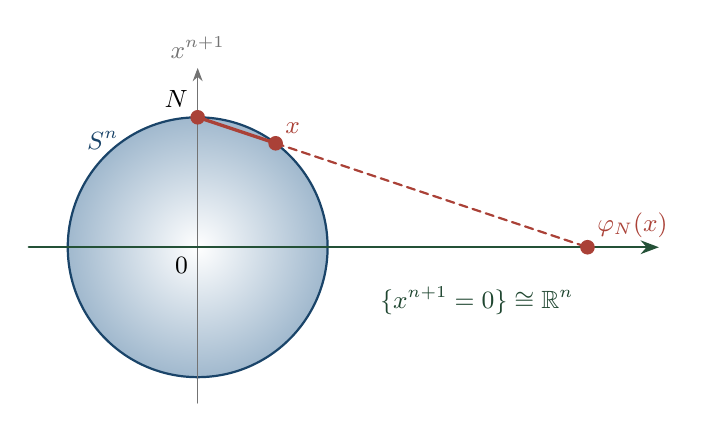
\begin{tikzpicture}[>=Stealth,scale=1.65,line cap=round,line join=round]
\shade[inner color=white,outer color=manifoldblue!43] (0,0) circle (1);
\draw[manifoldblue!75!black,thick] (0,0) circle (1);
\draw[->,black!55] (0,-1.2)--(0,1.38) node[above,font=\small] {$x^{n+1}$};
\draw[->,manifoldgreen!65!black,thick] (-1.3,0)--(3.55,0);
\node[below,font=\small,manifoldgreen!55!black] at (2.15,-.23)
 {$\{x^{n+1}=0\}\cong\R^n$};
\coordinate (N) at (0,1);
\coordinate (X) at (.6,.8);
\coordinate (P) at (3,0);
\draw[manifoldred,very thick] (N)--(X);
\draw[manifoldred,thick,densely dashed] (X)--(P);
\foreach \name in {N,X,P}{\fill[manifoldred] (\name) circle (1.6pt);}
\node[above left,font=\small] at (N) {$N$};
\node[above right,font=\small,manifoldred] at (X) {$x$};
\node[above right,font=\small,manifoldred] at (P) {$\varphi_N(x)$};
\node[below left,font=\small] at (0,0) {$0$};
\node[manifoldblue!75!black,font=\small] at (-.73,.82) {$S^n$};
\end{tikzpicture}
\caption{Rzut stereograficzny na płaszczyznę równikową, zgodny ze wzorem
w tekście. Pokazano przekrój płaszczyzną zawierającą oś biegunową
i punkt $x$. Punkty $N,x,\varphi_N(x)$ leżą na jednej prostej;
punkt przecięcia z $\{x^{n+1}=0\}$ ma współrzędne
$\varphi_N(x)=(x^1,\ldots,x^n)/(1-x^{n+1})$.}
\label{fig:stereo}
\end{figure}


\begin{przyklad}[Rzeczywista przestrzeń rzutowa]\label{prz:RPn}
Niech $\R_*:=\R\setminus\{0\}$ oznacza zbiór niezerowych
liczb rzeczywistych.
Niech $\mathbb{RP}^n = (\R^{n+1}\setminus\{0\})/\!\sim$,
gdzie
\[
x\sim y
\iff
\exists\,\lambda\in\R_*
\quad\text{takie, że}\quad
x=\lambda y.
\]
Przestrzeń $\mathbb{RP}^n$ wyposażamy w topologię ilorazową względem
rzutowania
\[
\pi:\R^{n+1}\setminus\{0\}\longrightarrow\mathbb{RP}^n,
\qquad
\pi(x)=[x].
\]
Punkty przestrzeni rzutowej zapisujemy w postaci $[x^0:\dots:x^n]$.

Dla $i=0,\dots,n$ definiujemy $U_i = \{[x^0:\dots:x^n]\in\mathbb{RP}^n:x^i\neq0\}$.
Najpierw należy sprawdzić, że definicja ta nie zależy od wyboru
reprezentanta klasy $[x]$. Jeżeli $x\sim y$, to istnieje
$\lambda\neq0$ takie, że $y=\lambda x$, a więc $y^i=\lambda x^i$.
Ponieważ $\lambda\neq0$, mamy $x^i\neq0 \iff y^i\neq0$.
Warunek $x^i\neq0$ zależy zatem wyłącznie od klasy $[x]$, więc zbiór
$U_i$ jest dobrze określony.

Zauważmy następnie, że $\pi^{-1}(U_i) = \{x\in\R^{n+1}\setminus\{0\}:x^i\neq0\}$.
Jest to zbiór otwarty w $\R^{n+1}\setminus\{0\}$, ponieważ jest
przeciwobrazem otwartego zbioru
$\R_*$ przez ciągłą funkcję współrzędnościową $x\longmapsto x^i$.
Z definicji topologii ilorazowej zbiór $A\subseteq\mathbb{RP}^n$
jest otwarty wtedy i tylko wtedy, gdy $\pi^{-1}(A)$ jest otwarty
w $\R^{n+1}\setminus\{0\}$. Stąd każdy $U_i$ jest otwarty.

Ponieważ każdy niezerowy wektor
$x=(x^0,\dots,x^n)$ ma przynajmniej jedną niezerową współrzędną,
zbiory $U_i$ pokrywają całą przestrzeń:
\[
\mathbb{RP}^n
=
\bigcup_{i=0}^n U_i.
\]

Na $U_i$ definiujemy odwzorowanie $\varphi_i:U_i\longrightarrow\R^n$
wzorem
\[
\varphi_i([x^0:\dots:x^n])
=
\left(
\frac{x^0}{x^i},
\dots,
\frac{x^{i-1}}{x^i},
\frac{x^{i+1}}{x^i},
\dots,
\frac{x^n}{x^i}
\right),
\]
czyli po znormalizowaniu reprezentanta tak, aby jego $i$-ta
współrzędna była równa $1$, pomijamy tę współrzędną.

Także tutaj należy sprawdzić niezależność od wyboru reprezentanta.
Jeżeli $y=\lambda x$ dla pewnego $\lambda\neq0$, to dla każdego
$j\neq i$ mamy $\frac{y^j}{y^i} = \frac{\lambda x^j}{\lambda x^i} = \frac{x^j}{x^i}$.
Wartość $\varphi_i([x])$ zależy więc wyłącznie od klasy $[x]$.

Odwzorowanie odwrotne jest dane jawnie przez wstawienie $1$
na $i$-te miejsce:
\[
\varphi_i^{-1}
(u^0,\dots,u^{i-1},u^{i+1},\dots,u^n)
=
[u^0:\dots:u^{i-1}:1:u^{i+1}:\dots:u^n].
\]
W szczególności $\varphi_i$ jest bijekcją.

Odwrotność $\varphi_i^{-1}$ jest ciągła, ponieważ jest złożeniem
ciągłego odwzorowania
\[
(u^0,\dots,u^{i-1},u^{i+1},\dots,u^n)
\longmapsto
(u^0,\dots,u^{i-1},1,u^{i+1},\dots,u^n)
\]
z ciągłym rzutowaniem ilorazowym $\pi$.

Aby wykazać ciągłość $\varphi_i$, zauważmy, że na zbiorze $\pi^{-1}(U_i)=\{x^i\neq0\}$
mamy
\[
\varphi_i\circ\pi(x)
=
\left(
\frac{x^0}{x^i},
\dots,
\frac{x^{i-1}}{x^i},
\frac{x^{i+1}}{x^i},
\dots,
\frac{x^n}{x^i}
\right),
\]
a więc $\varphi_i\circ\pi$ jest ciągłe. Ponieważ obcięcie $\pi|_{\pi^{-1}(U_i)}: \pi^{-1}(U_i)\longrightarrow U_i$
jest odwzorowaniem ilorazowym, wynika stąd ciągłość $\varphi_i$.
Otrzymujemy zatem homeomorfizm $\varphi_i:U_i\longrightarrow\R^n$.

Pozostaje sprawdzić zgodność map. Dla $i\neq j$ na przecięciu
$U_i\cap U_j$ odwzorowanie przejścia $\varphi_j\circ\varphi_i^{-1}$
jest określone tam, gdzie współrzędna odpowiadająca ilorazowi
$x^j/x^i$ jest niezerowa. Każda jego składowa jest albo odwrotnością
tej współrzędnej, albo ilorazem jednej ze współrzędnych przez nią.
Są to zatem funkcje wymierne o nieznikającym na dziedzinie
mianowniku, a więc funkcje gładkie.

W konsekwencji $\{(U_i,\varphi_i)\}_{i=0}^n$
jest atlasem gładkim. Po sprawdzeniu aksjomatów topologicznych
w twierdzeniu poniżej otrzymujemy, że $\mathbb{RP}^n$ jest
rozmaitością gładką wymiaru $n$.
\end{przyklad}


\begin{przyklad}[Dwie mapy $\mathbb{RP}^2$ krok po kroku]\label{prz:RP2-przejscie-1}
Na $U_0$ każda klasa ma jednoznacznego reprezentanta $[1:u:v]$,
natomiast na $U_1$ ma reprezentanta $[a:1:b]$.
Ich część wspólna $U_0\cap U_1$, zapisana we współrzędnych mapy
$\varphi_0$, odpowiada warunkowi $u\neq0$. Aby przejść od współrzędnych
zadanych przez $\varphi_0$ do współrzędnych zadanych przez $\varphi_1$,
dzielimy trzy współrzędne jednorodne przez $u$: $[1:u:v] = [1/u:1:v/u]$.
Stąd odwzorowanie zmiany współrzędnych ma postać $\varphi_1\circ\varphi_0^{-1}(u,v) = \left(\frac1u,\frac vu\right)$.
Oznacza to, że jeżeli punkt $p\in U_0\cap U_1$ ma w pierwszej mapie
współrzędne $\varphi_0(p)=(u,v)$,
to w drugiej mapie jego współrzędne wynoszą $\varphi_1(p)=(a,b) = \left(\frac1u,\frac vu\right)$.

Dziedziną odwzorowania przejścia jest $\{(u,v)\in\R^2:u\neq0\}$,
a jego macierz Jacobiego wynosi
\[
D(\varphi_1\circ\varphi_0^{-1})(u,v)
=
\begin{pmatrix}
-u^{-2} & 0\\[1mm]
-vu^{-2} & u^{-1}
\end{pmatrix}.
\]
Ponieważ $\det D(\varphi_1\circ\varphi_0^{-1})(u,v) = -u^{-3}\neq0$,
a odwrotne przejście ma postać $(a,b)\longmapsto \left(\frac1a,\frac ba\right)$,
odwzorowanie przejścia jest dyfeomorfizmem.

Zmianę współrzędnych wektora stycznego w tych mapach obliczymy
w przykładzie~\ref{prz:RP2-styczna-1}, po zdefiniowaniu przestrzeni stycznej.
\end{przyklad}


\begin{uwaga}[Geometryczna interpretacja $\mathbb{RP}^1$ i $\mathbb{RP}^2$]
Przestrzeń $\mathbb{RP}^n$ można interpretować jako zbiór prostych
przechodzących przez początek układu współrzędnych w $\R^{n+1}$.
Rzeczywiście, punkt $[x^0:\dots:x^n]\in\mathbb{RP}^n$
odpowiada prostej $\ell_x=\{\lambda x:\lambda\in\R\}$.
Zmiana reprezentanta $x$ na $\mu x$, gdzie $\mu\neq0$, nie zmienia tej
prostej. Współrzędne jednorodne opisują więc nie konkretny punkt
$\R^{n+1}$, lecz kierunek prostej przechodzącej przez $0$.

Każda taka prosta przecina sferę jednostkową $S^n$ w dokładnie dwóch
punktach antypodalnych $x$ i $-x$. Stąd $\mathbb{RP}^n\cong S^n/\{x\sim-x\}$.
Jest to także identyfikacja topologii. Oznaczmy pierwotne rzutowanie
przez $\pi$ i jego ograniczenie do sfery przez $q$.
Normalizacja $\nu(x)=x/\|x\|$ jest ciągła i $\pi=q\circ\nu$.
Jeśli $q^{-1}(A)$ jest otwarty w sferze, to
$\pi^{-1}(A)=\nu^{-1}(q^{-1}(A))$ jest otwarty, zatem $A$ jest
otwarty w pierwotnej topologii ilorazowej. Odwrotna implikacja
wynika z ciągłości $q$. Stąd $q$ jest odwzorowaniem ilorazowym,
co uzasadnia powyższy homeomorfizm.

Dla $n=1$ otrzymujemy $\mathbb{RP}^1\cong S^1/\{z\sim-z\}$.
Po utożsamieniu $S^1$ z okręgiem jednostkowym w $\C$ rozważmy
odwzorowanie $F:S^1\to S^1,\ F(z)=z^2$.
Ponieważ $F(z)=F(-z)$,
odwzorowanie to jest stałe na parach antypodalnych i wyznacza
odwzorowanie $\widetilde F:\mathbb{RP}^1\to S^1, \ \widetilde F([z])=z^2$.
Jest ono bijekcją, ponieważ $z^2=w^2 \iff z=\pm w$,
a każdy punkt okręgu posiada dwa przeciwne pierwiastki kwadratowe.
Ciągłość $\widetilde F$ wynika z ciągłości $F=\widetilde F\circ q$
i własności ilorazu. Ponieważ $\mathbb{RP}^1=q(S^1)$ jest zwarta,
a $S^1$ jest przestrzenią Hausdorffa, $\widetilde F$ jest homeomorfizmem.

Jest to również dyfeomorfizm. Jeśli $z=e^{i\theta}$,
to w $\mathbb{RP}^1$ kąty $\theta$ i $\theta+\pi$ opisują ten sam punkt,
natomiast $\widetilde F([e^{i\theta}])=e^{2i\theta}$.
Sprawdźmy zgodność współrzędnych kątowych z podanym wcześniej atlasem.
Dla $[\cos\theta:\sin\theta]$, na małym przedziale z $\cos\theta\ne0$,
współrzędną afiniczną jest $\tan\theta$, o pochodnej $1/\cos^2\theta$.
Gdy $\sin\theta\ne0$, druga mapa daje $\cot\theta$, o pochodnej
$-1/\sin^2\theta$. Pochodne nie znikają, więc przejścia i ich lokalne
odwrotności są gładkie. Kąt jest zatem zgodną lokalną współrzędną.
W lokalnych współrzędnych kątowych odwzorowanie ma więc postać $\theta\longmapsto 2\theta$,
a jego lokalna odwrotność $\alpha\longmapsto \frac{\alpha}{2}$.
Oba odwzorowania są gładkie, zatem $\mathbb{RP}^1\cong S^1$
jako rozmaitości gładkie.

Dla $n=2$ otrzymujemy $\mathbb{RP}^2\cong S^2/\{x\sim-x\}$.
Możemy ograniczyć się do domkniętej półsfery północnej. Każda para
antypodalna spoza równika ma dokładnie jeden punkt w jej wnętrzu; na równiku
oba punkty pary należą do półsfery. Ponieważ domknięta półsfera jest
homeomorficzna z dyskiem $D^2$, otrzymujemy model $\mathbb{RP}^2 \cong D^2/\{x\sim-x\text{ dla }x\in\partial D^2\}$.
Oznacza to, że punkty wewnętrzne dysku pozostają różne, natomiast każdy
punkt brzegu utożsamiamy z punktem antypodalnym. Rzutowanie półsfery
na $\mathbb{RP}^2$ jest ciągłą surjekcją i ma dokładnie te włókna.
Wyznacza zatem ciągłą bijekcję z opisanego ilorazu dysku.
Jej dziedzina jest zwarta, a $\mathbb{RP}^2$ jest przestrzenią Hausdorffa
na mocy twierdzenia~\ref{thm:rzutowe-zwarte-1}; jest więc homeomorfizmem.

Model ten daje również intuicję, dlaczego $\mathbb{RP}^2$ nie jest
orientowalna. Wyobraźmy sobie małą strzałkę lub niewielką figurę
asymetryczną przesuwaną po dysku. Gdy dochodzimy do brzegu, przechodzimy
przez niego dzięki utożsamieniu z punktem leżącym po przeciwnej stronie
okręgu. Po takim przejściu kierunek wzdłuż brzegu pozostaje zgodny,
natomiast kierunek wskazujący do wnętrza dysku zostaje odwrócony.

Lokalnie można to zapisać schematycznie jako $(s,t)\longmapsto (s,-t)$,
gdzie $s$ oznacza kierunek wzdłuż brzegu, a $t$ kierunek poprzeczny.
Jedna z dwóch lokalnych współrzędnych zmienia więc zwrot. Po przejściu
wzdłuż odpowiedniej zamkniętej drogi wracamy do punktu początkowego
z odwróconą lokalną orientacją. Nie można zatem wybrać orientacji
w sposób zgodny na całej przestrzeni.

Jest to geometryczna intuicja nieorientowalności $\mathbb{RP}^2$;
formalny dowód podamy po wprowadzeniu pojęcia orientacji rozmaitości.
\end{uwaga}


\begin{figure}[h]
\centering
\begin{tikzpicture}[>=Stealth,scale=1]

  %-------------------- RP^1 --------------------
  \begin{scope}
    % Okrąg
    \draw[thick,manifoldblue] (0,0) circle (1.45);

    % Kilka par antypodalnych na okręgu
    \foreach \ang in {0,45,90,135}{
        \draw[dashed,gray!55]
            (\ang:1.45) -- ({\ang+180}:1.45);

        \fill[manifoldgold]
            (\ang:1.45) circle (2.2pt);
        \fill[manifoldgold]
            ({\ang+180}:1.45) circle (2.2pt);
    }

    % Wyróżniona para x i -x
    \fill[manifoldred] (20:1.45) circle (2.8pt);
    \fill[manifoldred] (200:1.45) circle (2.8pt);

    \node[manifoldred, above right] at (20:1.45) {$x$};
    \node[manifoldred, below left] at (200:1.45) {$-x$};

    % Strzałka pokazująca utożsamienie wyróżnionej pary
    \draw[<->,thick,manifoldred]
      (20:1.36) to[bend left=18] (200:1.36);

    % Opisy
    \node[manifoldblue] at (0,1.85) {$S^1$};

    \node[align=center,manifoldred] at (0,-1.95)
      {$x\sim -x$ dla każdego $x\in S^1$};

    \node at (0,-2.35)
      {$\displaystyle \mathbb{RP}^1\cong S^1/\{x\sim -x\}$};

    \node at (0,-2.75)
      {$\displaystyle \cong\, S^1$};
  \end{scope}

  %-------------------- RP^2 --------------------
  \begin{scope}[xshift=6.2cm]
    % Dysk
    \fill[manifoldblue!8] (0,0) circle (1.45);
    \draw[thick,manifoldblue] (0,0) circle (1.45);

    % Kilka przykładowych par punktów antypodalnych na brzegu
    \foreach \ang in {0,45,90,135}{
        \fill[manifoldgold]
            (\ang:1.45) circle (2.2pt);
        \fill[manifoldgold]
            ({\ang+180}:1.45) circle (2.2pt);
    }

    % Wyróżniona para x i -x
    \fill[manifoldred] (0:1.45) circle (2.8pt);
    \fill[manifoldred] (180:1.45) circle (2.8pt);

    \node[manifoldred, right] at (0:1.45) {$x$};
    \node[manifoldred, left]  at (180:1.45) {$-x$};

    % Strzałka pokazująca utożsamienie
    \draw[<->,thick,manifoldred]
        (1.36,0) to[bend left=20] (-1.36,0);
    \node[align=center,font=\scriptsize,manifoldblue] at (0,0.55)
        {wnętrze bez\\utożsamień};

    % Opisy
    \node[manifoldblue] at (0,1.85) {$D^2$};

    \node[align=center,manifoldred] at (0,-1.95)
        {$x\sim -x$ dla każdego $x\in\partial D^2$};

    \node at (0,-2.35)
        {$\displaystyle \mathbb{RP}^2
        \cong D^2/\{x\sim -x,\;x\in\partial D^2\}$};
  \end{scope}

\end{tikzpicture}
\caption{Dwa użyteczne modele przestrzeni rzutowych.
Po lewej, $\mathbb{RP}^1$ otrzymujemy z okręgu $S^1$ przez utożsamienie
par antypodalnych punktów. Po prawej, $\mathbb{RP}^2$ otrzymujemy z dysku
$D^2$ przez utożsamienie antypodalnych punktów jego brzegu. Różnica polega
na tym, że w pierwszym przypadku utożsamiamy punkty na całym okręgu,
natomiast w drugim utożsamienie zachodzi tylko na brzegu dysku.}
\label{fig:projective-models}
\end{figure}


\begin{twierdzenie}[Przestrzenie rzutowe jako zwarte rozmaitości]\label{thm:rzutowe-zwarte-1}
Przestrzeń $\mathbb{RP}^n$ jest zwartą rozmaitością gładką wymiaru $n$, a
$\mathbb{CP}^n$ jest zwartą rozmaitością zespoloną wymiaru $n$ (a więc zwartą
rozmaitością rzeczywistą wymiaru $2n$).
\end{twierdzenie}

\begin{proof}
Zaczniemy od zwartości. Niech
\[
\pi_{\R}:\R^{n+1}\setminus\{0\}\longrightarrow\mathbb{RP}^n,
\qquad
\pi_{\R}(x)=[x],
\]
będzie rzutowaniem ilorazowym. Ograniczając je do sfery jednostkowej,
otrzymujemy ciągłe odwzorowanie $q_{\R}:S^n\longrightarrow\mathbb{RP}^n, \ q_{\R}(x)=[x]$.
Jest ono surjektywne. Istotnie, jeśli $[x]\in\mathbb{RP}^n$,
to $x\neq0$ i możemy znormalizować reprezentanta: $\widehat{x}:=\frac{x}{\|x\|}\in S^n$.
Ponieważ $\widehat{x}$ jest niezerową wielokrotnością $x$, mamy $[\widehat{x}]=[x]$.
Każdy punkt $\mathbb{RP}^n$ należy więc do obrazu $q_{\R}$.

Sfera $S^n$ jest zwarta, a ciągły obraz przestrzeni zwartej jest zwarty.
Ponieważ $q_{\R}(S^n)=\mathbb{RP}^n$,
otrzymujemy, że $\mathbb{RP}^n$ jest zwarta.

Dokładnie ten sam argument działa w przypadku zespolonym. Niech
\[
\pi_{\C}:\C^{n+1}\setminus\{0\}\longrightarrow\mathbb{CP}^n,
\qquad
\pi_{\C}(z)=[z].
\]
Po utożsamieniu $\C^{n+1}\cong\R^{2n+2}$ sfera jednostkowa ma postać $S^{2n+1} = \{z\in\C^{n+1}:\|z\|=1\}$.
Ograniczenie $q_{\C}:S^{2n+1}\longrightarrow\mathbb{CP}^n, \ q_{\C}(z)=[z]$,
jest ciągłe i surjektywne, ponieważ dla każdego $[z]\in\mathbb{CP}^n$
wektor $\widehat{z}:=\frac{z}{\|z\|}$
należy do $S^{2n+1}$ i reprezentuje tę samą klasę: $[\widehat{z}]=[z]$.
Ponieważ $S^{2n+1}$ jest zwarta, jej ciągły obraz $q_{\C}(S^{2n+1})=\mathbb{CP}^n$
jest zwarty. Zatem również $\mathbb{CP}^n$ jest zwarta.

Sprawdźmy teraz aksjomat Hausdorffa bez powoływania się na ogólne
twierdzenie o ilorazach. Dla jednostkowych reprezentantów $x,y\in S^n$
dwóch klas rzeczywistych połóżmy $d_{\R}([x],[y]) = \min\{\|x-y\|,\|x+y\|\}$.
Dla jednostkowych reprezentantów $z,w\in S^{2n+1}$ połóżmy $d_{\C}([z],[w]) = \min_{|\lambda|=1}\|z-\lambda w\|$.
Oba wzory nie zależą od wyboru jednostkowych reprezentantów:
w przypadku rzeczywistym zmiana $x$ na $-x$ jedynie zamienia miejscami
dwie liczby występujące w minimum, natomiast w przypadku zespolonym
zmiana reprezentanta przez czynnik o module $1$ jedynie zmienia
parametryzację zbioru, po którym bierzemy minimum. Minima istnieją
dzięki zwartości grup $\{\pm1\}$ i $S^1$.

Nierówność trójkąta sprawdzimy jednocześnie dla obu przypadków,
pisząc $G=\{\pm1\}$ lub $G=S^1$. Dla jednostkowych $x,y,z$
wybierzmy $\lambda,\mu\in G$ realizujące minima dla par $(x,y)$ i $(y,z)$.
Ponieważ mnożenie przez $\lambda$ zachowuje normę,
\begin{align*}
d([x],[z])&\leq\|x-\lambda\mu z\|\\
&\leq\|x-\lambda y\|+\|\lambda y-\lambda\mu z\|\\
&=d([x],[y])+d([y],[z]).
\end{align*}
Symetria wynika z zastąpienia $\lambda$ przez $\lambda^{-1}$.
Ponadto osiągane minimum jest równe zeru wtedy i tylko wtedy,
gdy reprezentanty należą do tej samej orbity, czyli reprezentują
ten sam punkt przestrzeni rzutowej. Otrzymujemy więc metryki na zbiorach klas.

Pozostaje sprawdzić, że topologie wyznaczone przez te metryki są
topologiami ilorazowymi. Rzutowania
\[
q_{\R}:S^n\to(\mathbb{RP}^n,d_{\R}),
\qquad
q_{\C}:S^{2n+1}\to(\mathbb{CP}^n,d_{\C})
\]
są ciągłe, ponieważ odległość klas nie przekracza odległości ich
wybranych reprezentantów. Aby przejść od sfer do pierwotnych ilorazów,
używamy ciągłej normalizacji $\nu(v)=v/\|v\|$.
Rzutowania $\pi_{\R}$ i $\pi_{\C}$ do przestrzeni klas z metryką są ciągłe,
bo mają postać $q_{\R}\circ\nu$ i $q_{\C}\circ\nu$.
Z definicji topologii ilorazowej wynika więc ciągłość identyczności
z pierwotnego ilorazu do przestrzeni metrycznej.
Z drugiej strony mamy już wykazaną zwartość
$\mathbb{RP}^n$ i $\mathbb{CP}^n$ w ich topologiach ilorazowych.
Identyczność z przestrzeni rzutowej wyposażonej w topologię ilorazową
do tego samego zbioru klas wyposażonego w powyższą metrykę jest więc
ciągłą bijekcją ze zwartej przestrzeni do przestrzeni Hausdorffa.
Jest zatem homeomorfizmem. W szczególności pierwotna topologia
ilorazowa jest Hausdorffa.

Każda z przestrzeni rzutowych ma skończony atlas $U_0,\ldots,U_n$,
którego obrazy są równe odpowiednio $\R^n$ lub $\C^n$. Wybierzmy
w $\R^n$ oraz $\C^n\cong\R^{2n}$ przeliczalną bazę, na przykład
złożoną z kul o wymiernych środkach i wymiernych promieniach.
Przeciwobrazy tych baz przez skończenie wiele map atlasu tworzą
przeliczalną bazę przestrzeni rzutowej.

Odwzorowania przejścia są ilorazami współrzędnych przez współrzędną
niezerową, a więc są gładkie w przypadku rzeczywistym i holomorficzne
w przypadku zespolonym. Otrzymujemy zatem strukturę rozmaitości
gładkiej wymiaru $n$ na $\mathbb{RP}^n$ oraz strukturę rozmaitości
zespolonej wymiaru $n$ na $\mathbb{CP}^n$. Ponieważ $\C^n\cong\R^{2n}$,
$\mathbb{CP}^n$ ma jako rozmaitość rzeczywista wymiar $2n$.
\end{proof}


\begin{uwaga}
Zwartość można zobaczyć bardzo bezpośrednio: każde $\mathbb{RP}^n$ jest ilorazem
sfery $S^n$ przez relację $x\sim-x$, a $\mathbb{CP}^n$ jest ilorazem sfery
jednostkowej $S^{2n+1}\subset\C^{n+1}$ przez działanie grupy $S^1$, $z\sim e^{i\theta}z$.
W przypadku zespolonym otrzymujemy w ten sposób słynną fibrację Hopfa
$S^1\longrightarrow S^{2n+1}\longrightarrow\mathbb{CP}^n$.
Pełny opis tej konstrukcji wykracza poza zakres tego rozdziału, ale pokazuje,
że przestrzenie rzutowe są naturalnie związane zarówno z ilorazami, jak i z teorią
wiązek.
\end{uwaga}

\begin{przyklad}[Torus $T^n$]\label{prz:torus}
Niech $T^n=\R^n/\Z^n$ z topologią ilorazową względem rzutowania kanonicznego $\pi\colon\R^n
\to T^n$, $\pi(x)=x+\Z^n$. Pokażemy najpierw, że $\pi$ jest odwzorowaniem otwartym: dla
zbioru otwartego $\Omega\subseteq\R^n$, $\pi^{-1}(\pi(\Omega))=\bigcup_{k\in\Z^n}(\Omega+k)$
jest sumą zbiorów otwartych, a więc otwarty; z definicji topologii ilorazowej oznacza to,
że $\pi(\Omega)$ jest otwarty w $T^n$.

Sprawdźmy pozostałe warunki topologiczne. Jeśli $[x]\ne[y]$, to
$\delta=\inf_{k\in\Z^n}\|x-y-k\|>0$: w dowolnym ograniczonym
zbiorze jest tylko skończenie wiele punktów kraty, a $x-y\notin\Z^n$.
Otwarte otoczenia $\pi(B(x,\delta/3))$ i $\pi(B(y,\delta/3))$
są rozłączne. W przeciwnym razie istniałyby $u,v$ w tych kulach
z $u-v=k\in\Z^n$, skąd $\|x-y-k\|<2\delta/3$, sprzeczność.
Torus jest więc Hausdorffa. Obrazy przeliczalnej bazy kul w $\R^n$
stanowią bazę ilorazu: dla otwartego $O\subset T^n$ i $[x]\in O$
wybieramy kulę bazową $B$ z $x\in B\subset\pi^{-1}(O)$;
wtedy $[x]\in\pi(B)\subset O$. To daje drugi aksjomat przeliczalności.

Niech $B(x,1/2)\subseteq\R^n$ będzie kulą otwartą o promieniu $1/2$. Dla $k\in\Z^n\setminus
\{0\}$, zbiory $B(x,1/2)$ i $B(x+k,1/2)$ są rozłączne: gdyby $y$ należał do obu, to
$\|y-x\|<1/2$ i $\|y-x-k\|<1/2$, skąd z nierówności trójkąta $\|k\|\leq\|y-x\|+\|y-x-k\|<1$;
ale $\|k\|\geq1$ dla $k\in\Z^n\setminus\{0\}$ — sprzeczność. Zatem $\pi|_{B(x,1/2)}$ jest
różnowartościowe, a więc — jako odwzorowanie ciągłe, otwarte i różnowartościowe na obraz —
homeomorfizmem $B(x,1/2)\to\pi(B(x,1/2))$. Kładziemy $\varphi_x:=(\pi|_{B(x,1/2)})^{-1}$;
zbiory $\pi(B(x,1/2))$ dla $x\in\R^n$ pokrywają $T^n$.

Odwzorowania przejścia między takimi mapami są (lokalnie) postaci $y\mapsto y+k$ dla
pewnego ustalonego $k\in\Z^n$ (bo dwa punkty z tym samym obrazem przy $\pi$ różnią się
dokładnie o wektor z $\Z^n$, a $k$ jest lokalnie stałe z ciągłości) — a translacja jest
odwzorowaniem gładkim z gładką odwrotną. Zatem otrzymana rodzina map jest atlasem, i $T^n$
jest rozmaitością gładką wymiaru $n$.
\end{przyklad}
\section{Przestrzeń styczna}\label{sec:przestrzen-styczna}

W porównaniu trzech poniższych modeli zakładamy,
że $M$ nie ma brzegu. Dla punktów brzegu
przestrzeń styczną definiujemy przez derywacje
lub współrzędne przedłużane poza półprzestrzeń,
jak w Sekcji~\ref{sec:rozmaitosci-z-brzegiem-1};
model dwustronnych krzywych nie działa tam dosłownie.

Chcemy nadać sens pojęciu ,,wektora stycznego'' do rozmaitości $M$ w punkcie $p$ —
uogólnieniu intuicji wektora stycznego do powierzchni w $\R^3$, niezależnemu od
zanurzenia $M$ w jakąkolwiek przestrzeń otaczającą. Istnieje kilka naturalnych, a priori
różnych, sposobów sformalizowania tej intuicji; w tej sekcji podajemy trzy z nich i
dowodzimy, że są one kanonicznie równoważne.

\subsection*{Trzy definicje przestrzeni stycznej}

Niech $M$ będzie rozmaitością gładką wymiaru $n$, $p\in M$.

\paragraph*{Definicja A (poprzez krzywe).} Niech $\Gamma_p$ oznacza zbiór gładkich krzywych
$\gamma\colon(-\varepsilon,\varepsilon)\to M$ (dla pewnego $\varepsilon>0$, zależnego od
$\gamma$) z $\gamma(0)=p$. Mówimy, że $\gamma_1,\gamma_2\in\Gamma_p$ są \emph{styczne w
$p$}, $\gamma_1\sim\gamma_2$, jeśli dla pewnej (równoważnie: każdej) mapy dopuszczalnej
$(U,\varphi)$ wokół $p$,
\[
(\varphi\circ\gamma_1)'(0)=(\varphi\circ\gamma_2)'(0)\quad\text{w }\R^n.
\]

\begin{figure}[!ht]
\centering
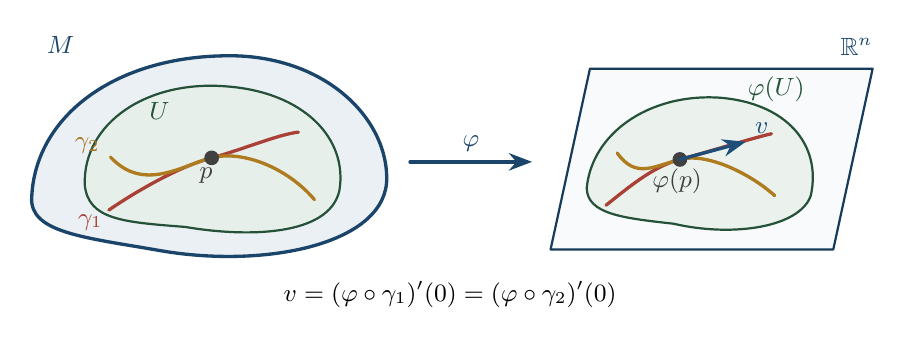
\begin{tikzpicture}[>=Stealth,scale=1.02,line cap=round,line join=round]
% Dwie różne krzywe, których pochodne w p po przejściu do współrzędnych są równe.
\filldraw[fill=manifoldblue!9,draw=manifoldblue!75!black,very thick]
 (-5.04,-.52) .. controls (-5.0,.46) and (-4.05,1.21) .. (-2.67,1.24)
 .. controls (-1.44,1.28) and (-.63,.5) .. (-.62,-.27)
 .. controls (-.6,-1.1) and (-2.13,-1.42) .. (-3.47,-1.18)
 .. controls (-4.39,-1.02) and (-5.07,-.96) .. cycle;
\filldraw[fill=manifoldgreen!12,draw=manifoldgreen!65!black,thick]
 (-4.38,-.36) .. controls (-4.4,.4) and (-3.61,.94) .. (-2.62,.86)
 .. controls (-1.65,.79) and (-1.1,.21) .. (-1.21,-.44)
 .. controls (-1.34,-1.01) and (-2.37,-1.02) .. (-3.13,-.89)
 .. controls (-3.91,-.83) and (-4.34,-.8) .. cycle;
\node[font=\small\bfseries,manifoldblue!75!black] at (-4.68,1.37) {$M$};
\node[font=\small,manifoldgreen!65!black] at (-3.45,.55) {$U$};
\draw[manifoldred,very thick]
 (-4.08,-.68) .. controls (-3.7,-.42) and (-3.18,-.13) .. (-2.8,-.03)
 .. controls (-2.42,.07) and (-1.98,.26) .. (-1.72,.29);
\draw[manifoldgold!85!black,very thick]
 (-4.06,-.02) .. controls (-3.65,-.46) and (-3.18,-.13) .. (-2.8,-.03)
 .. controls (-2.42,.07) and (-1.86,-.15) .. (-1.52,-.55);
\node[font=\small,manifoldred] at (-4.31,-.83) {$\gamma_1$};
\node[font=\small,manifoldgold!80!black] at (-4.35,.12) {$\gamma_2$};
\fill[black!75] (-2.8,-.03) circle (2.6pt)
 node[below,font=\small,xshift=-2pt] {$p$};
\draw[->,very thick,manifoldblue!75!black] (-.33,-.08)--(1.19,-.08)
 node[midway,above,font=\small] {$\varphi$};
% Rysunkowy fragment R^n oraz obraz U.
\filldraw[fill=manifoldblue!3,draw=manifoldblue!65!black,thick]
 (1.42,-1.17)--(4.94,-1.17)--(5.43,1.08)--(1.91,1.08)--cycle;
\filldraw[fill=manifoldgreen!10,draw=manifoldgreen!65!black,thick]
 (1.87,-.41) .. controls (1.93,.27) and (2.64,.77) .. (3.51,.72)
 .. controls (4.35,.66) and (4.8,.14) .. (4.66,-.5)
 .. controls (4.52,-.9) and (3.68,-1.02) .. (2.95,-.85)
 .. controls (2.32,-.78) and (1.88,-.73) .. cycle;
\draw[manifoldred,very thick]
 (2.11,-.62) .. controls (2.39,-.4) and (2.69,-.14) .. (3.03,-.05)
 .. controls (3.37,.04) and (3.91,.21) .. (4.17,.27);
\draw[manifoldgold!85!black,very thick]
 (2.25,.03) .. controls (2.48,-.29) and (2.69,-.14) .. (3.03,-.05)
 .. controls (3.37,.04) and (3.91,-.23) .. (4.21,-.5);
\fill[black!75] (3.03,-.05) circle (2.6pt)
 node[below,font=\small,xshift=-1pt] {$\varphi(p)$};
\draw[->,very thick,manifoldblue!85!black] (3.03,-.05)--(3.85,.17);
\node[font=\small,manifoldblue!85!black] at (4.05,.34) {$v$};
\node[font=\small,manifoldgreen!65!black] at (4.23,.82) {$\varphi(U)$};
\node[font=\small\bfseries,manifoldblue!75!black] at (5.23,1.35) {$\R^n$};
\node[font=\small] at (.17,-1.73)
 {$v=(\varphi\circ\gamma_1)'(0)=(\varphi\circ\gamma_2)'(0)$};
\end{tikzpicture}
\caption{Dwie krzywe w $M$ przechodzą przez $p$ i mają ten sam kierunek
styczny. W mapie $\varphi$ ich obrazy mają wspólną pochodną $v$ w $t=0$.}
\label{fig:krzywe-styczne-w-mapie}
\end{figure}

\begin{fakt}
Powyższy warunek nie zależy od wyboru mapy $(U,\varphi)$.
\end{fakt}
\begin{proof}
Jeśli $(V,\psi)$ jest inną mapą wokół $p$, to na wspólnej dziedzinie $\psi\circ\gamma_i=
(\psi\circ\varphi^{-1})\circ(\varphi\circ\gamma_i)$ blisko $t=0$, więc z reguły łańcucha
\[
(\psi\circ\gamma_i)'(0)=D(\psi\circ\varphi^{-1})(\varphi(p))\cdot(\varphi\circ\gamma_i)'(0),
\qquad i=1,2.
\]
Ponieważ $D(\psi\circ\varphi^{-1})(\varphi(p))$ jest tym samym przekształceniem liniowym
dla $i=1$ i $i=2$, równość $(\varphi\circ\gamma_1)'(0)=(\varphi\circ\gamma_2)'(0)$
implikuje $(\psi\circ\gamma_1)'(0)=(\psi\circ\gamma_2)'(0)$, i na odwrót (bo
$D(\psi\circ\varphi^{-1})(\varphi(p))$ jest odwracalne, jako różniczka dyfeomorfizmu).
\end{proof}

Relacja $\sim$ jest relacją równoważności na $\Gamma_p$ (natychmiast z definicji, poprzez
odpowiednie własności równości w $\R^n$). Definiujemy $T_p^AM:=\Gamma_p/\!\sim$.

Aby wyposażyć $T_p^AM$ w strukturę przestrzeni wektorowej, ustalmy mapę
$(U,\varphi)$ wokół $p$ i zdefiniujmy
\[
\Theta_\varphi:T_p^AM\longrightarrow\R^n,
\qquad
\Theta_\varphi([\gamma]):=(\varphi\circ\gamma)'(0).
\]
Odwzorowanie to jest dobrze określone i bijektywne. Różnowartościowość
wynika bezpośrednio z definicji relacji równoważności, natomiast
surjektywność z faktu, że dla dowolnego $v\in\R^n$ krzywa $\gamma(t)=\varphi^{-1}(\varphi(p)+tv)$,
określona dla dostatecznie małych $|t|$, spełnia $\gamma(0)=p, \ (\varphi\circ\gamma)'(0)=v$.

Za pomocą bijekcji $\Theta_\varphi$ przenosimy strukturę przestrzeni
wektorowej z $\R^n$ na $T_p^AM$, definiując
\[
[\gamma]+[\eta]
:=
\Theta_\varphi^{-1}
\bigl(\Theta_\varphi([\gamma])+\Theta_\varphi([\eta])\bigr)
\]
oraz
\[
a[\gamma]
:=
\Theta_\varphi^{-1}
\bigl(a\,\Theta_\varphi([\gamma])\bigr),
\qquad a\in\R.
\]
W szczególności mnożenie przez skalar można reprezentować przez
reparametryzację krzywej: $a[\gamma]=[t\mapsto\gamma(at)]$,
ponieważ $(\varphi\circ\gamma(at))'_{\,t=0} = a(\varphi\circ\gamma)'(0)$.
W ten sposób $\Theta_\varphi$ jest, z definicji, izomorfizmem liniowym
$T_p^AM\cong\R^n$.

\begin{fakt}
Struktura liniowa na $T_p^AM$ nie zależy od wyboru mapy $\varphi$.
\end{fakt}
\begin{proof}
Niech $(V,\psi)$ będzie inną mapą wokół $p$, $L:=D(\psi\circ\varphi^{-1})(\varphi(p))
\colon\R^n\to\R^n$. Z rachunku w poprzednim Fakcie, dla dowolnej krzywej $\gamma\in\Gamma_p$,
$\Theta_\psi([\gamma])=L(\Theta_\varphi([\gamma]))$, czyli $\Theta_\psi=L\circ\Theta_\varphi$.
Ponieważ $L$ jest izomorfizmem \emph{liniowym} (jako różniczka dyfeomorfizmu w punkcie),
struktury liniowe przeniesione na $T_p^AM$ przez $\Theta_\varphi$ i przez $\Theta_\psi=
L\circ\Theta_\varphi$ pokrywają się: liniowość $L$ gwarantuje, że dla dowolnych $[\gamma_1],
[\gamma_2]\in T_p^AM$, $a,b\in\R$, kombinacja $a[\gamma_1]+b[\gamma_2]$ wyznaczona przez
$\Theta_\varphi$ pokrywa się z kombinacją wyznaczoną przez $\Theta_\psi$. To kluczowa
obserwacja: liniowość różniczki odwzorowania przejścia gwarantuje, że mimo iż
$\Theta_\varphi\neq\Theta_\psi$, wyznaczona przez nie struktura wektorowa na $T_p^AM$ jest
jedna i ta sama.
\end{proof}

\paragraph*{Definicja B (klasyczna, poprzez pary mapa-wektor).} Rozważmy zbiór trójek
$(U,\varphi,v)$, gdzie $(U,\varphi)$ jest mapą dopuszczalną wokół $p$, a $v\in\R^n$.
Mówimy, że $(U,\varphi,v)\sim(V,\psi,w)$, jeśli $w=D(\psi\circ\varphi^{-1})(\varphi(p))\,v$.

\begin{fakt}
Powyższa relacja jest relacją równoważności.
\end{fakt}
\begin{proof}
Zwrotność: dla $\psi=\varphi$, $D(\id)=\id$, więc $v=v$. Symetria: jeśli $w=D(\psi\varphi^{-1})
(\varphi(p))v$, to stosując regułę łańcucha do $\varphi\circ\psi^{-1}=(\psi\circ
\varphi^{-1})^{-1}$ w punkcie $\psi(p)$, $D(\varphi\psi^{-1})(\psi(p))=\big[D(\psi\varphi^{-1})
(\varphi(p))\big]^{-1}$, skąd $v=D(\varphi\psi^{-1})(\psi(p))w$. Przechodniość: jeśli
$w=D(\psi\varphi^{-1})(\varphi(p))v$ i $u=D(\eta\psi^{-1})(\psi(p))w$, to z reguły łańcucha
zastosowanej do $\eta\circ\varphi^{-1}=(\eta\circ\psi^{-1})\circ(\psi\circ\varphi^{-1})$ w
punkcie $\varphi(p)$,
\[
D(\eta\varphi^{-1})(\varphi(p))=D(\eta\psi^{-1})(\psi(p))\cdot D(\psi\varphi^{-1})(\varphi(p)),
\]
a więc $D(\eta\varphi^{-1})(\varphi(p))v=D(\eta\psi^{-1})(\psi(p))w=u$, czyli
$(U,\varphi,v)\sim(W,\eta,u)$.
\end{proof}

Definiujemy $T_p^BM$ jako zbiór klas równoważności $[U,\varphi,v]$.
Strukturę przestrzeni wektorowej wprowadzamy wzorem $a[U,\varphi,v]+b[U,\varphi,v'] := [U,\varphi,av+bv']$.
Definicja ta jest dobrze określona, to znaczy wynik nie zależy od wyboru
reprezentantów klas. Istotnie, jeżeli przejdziemy do innej mapy
$(V,\psi)$ zawierającej punkt $p$, to wektory $v,v'\in\mathbb{R}^n$
przechodzą odpowiednio w
\[
D(\psi\circ\varphi^{-1})(\varphi(p))\,v
\qquad\text{oraz}\qquad
D(\psi\circ\varphi^{-1})(\varphi(p))\,v'.
\]
Z liniowości różniczki otrzymujemy
\[
D(\psi\circ\varphi^{-1})(\varphi(p))(av+bv')
=
a\,D(\psi\circ\varphi^{-1})(\varphi(p))v
+
b\,D(\psi\circ\varphi^{-1})(\varphi(p))v',
\]
a więc oba wybory reprezentantów prowadzą do tej samej klasy
równoważności.

Ustalmy teraz mapę $(U,\varphi)$ wokół punktu $p$. Definiujemy
odwzorowanie
\[
\Phi_\varphi\colon T_p^AM\longrightarrow T_p^BM,
\qquad
\Phi_\varphi([\gamma])
=
[U,\varphi,(\varphi\circ\gamma)'(0)].
\]
Odwzorowanie to jest dobrze określone, ponieważ jeżeli
$[\gamma]=[\eta]$ w $T_p^AM$, to z definicji relacji równoważności
krzywych mamy $(\varphi\circ\gamma)'(0) = (\varphi\circ\eta)'(0)$,
a zatem
\[
[U,\varphi,(\varphi\circ\gamma)'(0)]
=
[U,\varphi,(\varphi\circ\eta)'(0)].
\]

Żeby sprawdzić bijektywność, rozważmy odwzorowanie
\[
j_\varphi\colon\R^n\longrightarrow T_p^BM,
\qquad j_\varphi(v)=[U,\varphi,v].
\]
Jest ono liniowe na mocy definicji działań. Jest też
różnowartościowe: jeżeli $[U,\varphi,v]=[U,\varphi,w]$,
to relacja równoważności w tej samej mapie daje $v=w$.
Jest na, gdyż dla dowolnej klasy $[V,\psi,w]$ element $v=D(\varphi\circ\psi^{-1})(\psi(p))w$
spełnia $[V,\psi,w]=[U,\varphi,v]$. Ponieważ
$\Theta_\varphi$ jest liniową bijekcją, mamy
$\Phi_\varphi=j_\varphi\circ\Theta_\varphi$,
a więc $\Phi_\varphi$ również jest liniową bijekcją.
Zmiana mapy nie zmienia tego odwzorowania: dla $(V,\psi)$
reguła łańcucha i definicja relacji równoważności dają
$j_\psi\circ\Theta_\psi=j_\varphi\circ\Theta_\varphi$.
Otrzymujemy zatem kanoniczne utożsamienie $T_p^AM\cong T_p^BM$.
Od tej chwili obie te przestrzenie będziemy oznaczać wspólnym symbolem $T_p^{\mathrm{geom}}M$.

\paragraph*{Definicja C (algebraiczna, poprzez derywacje).} Niech $C^\infty(M)$ oznacza
przestrzeń funkcji gładkich $M\to\R$. \emph{Derywacją w punkcie $p$} nazywamy funkcjonał
liniowy $v\colon C^\infty(M)\to\R$ spełniający regułę Leibniza: $v(fg)=f(p)\,v(g)+g(p)\,v(f), \ f,g\in C^\infty(M)$.
Zbiór wszystkich derywacji w $p$ oznaczamy $T_p^CM$ — jest to podprzestrzeń liniowa
przestrzeni funkcjonałów liniowych na $C^\infty(M)$ (suma i wielokrotność derywacji
spełnia regułę Leibniza — sprawdzenie bezpośrednie).

W dalszej części skonstruujemy kanoniczny izomorfizm
$T_p^{\mathrm{geom}}M\to T_p^CM$. Utożsamimy w ten sposób
wszystkie trzy definicje i otrzymamy bazę przestrzeni
stycznej złożoną z pochodnych cząstkowych.

\subsection*{Lemat Hadamarda}

Poniższy lemat analityczny jest podstawowym narzędziem technicznym tej sekcji.

\begin{lemat}[Lemat Hadamarda]\label{lem:hadamard}
Niech $\Omega\subseteq\R^n$ będzie zbiorem otwartym, gwiaździstym względem $0$ (tzn.\
$tx\in\Omega$ dla wszystkich $x\in\Omega$, $t\in[0,1]$), i niech $f\in C^\infty(\Omega)$.
Wówczas istnieją funkcje $g_1,\dots,g_n\in C^\infty(\Omega)$ takie, że
\[
f(x)=f(0)+\sum_{i=1}^nx^ig_i(x), \qquad x\in\Omega,
\]
oraz $g_i(0)=\dfrac{\partial f}{\partial x^i}(0)$ dla każdego $i$.
\end{lemat}

\begin{proof}
Dla ustalonego $x\in\Omega$, funkcja $t\mapsto f(tx)$ jest dobrze określona i gładka na
$[0,1]$ (bo $\Omega$ jest gwiaździsty względem $0$), więc z twierdzenia podstawowego
rachunku różniczkowego,
\[
f(x)-f(0)=\int_0^1\frac{d}{dt}f(tx)\,dt=\int_0^1\sum_{i=1}^n\frac{\partial f}{\partial x^i}
(tx)\,x^i\,dt=\sum_{i=1}^nx^i\underbrace{\int_0^1\frac{\partial f}{\partial x^i}(tx)\,dt}
_{=:g_i(x)}.
\]
Funkcje $g_i(x):=\int_0^1\frac{\partial f}{\partial x^i}(tx)\,dt$ są gładkie na $\Omega$
(różniczkowanie pod znakiem całki, dopuszczalne, gdyż funkcja podcałkowa zależy gładko od
$(t,x)$), oraz $g_i(0)=\int_0^1\frac{\partial f}{\partial x^i}(0)\,dt=\frac{\partial f}
{\partial x^i}(0)$, co kończy dowód.
\end{proof}

\subsection*{Od krzywych do derywacji}

Zdefiniujmy odwzorowanie $\Phi\colon T_p^AM\to T_p^CM$ wzorem
$\Phi([\gamma])(f):=(f\circ\gamma)'(0), \ f\in C^\infty(M)$.

\begin{fakt}
$\Phi$ jest dobrze określone (niezależne od wyboru reprezentanta $\gamma$), a
$\Phi([\gamma])$ jest derywacją w $p$ dla każdego $[\gamma]\in T_p^AM$.
\end{fakt}
\begin{proof}
Niezależność od reprezentanta: jeśli $\gamma_1\sim\gamma_2$, to pisząc $f\circ\gamma_i=
(f\circ\varphi^{-1})\circ(\varphi\circ\gamma_i)$ dla mapy $(U,\varphi)$ wokół $p$,
\[
(f\circ\gamma_i)'(0)=D(f\circ\varphi^{-1})(\varphi(p))\cdot(\varphi\circ\gamma_i)'(0),
\]
a prawa strona zależy od $\gamma_i$ jedynie poprzez $(\varphi\circ\gamma_i)'(0)$, które z
założenia $\gamma_1\sim\gamma_2$ jest tym samym wektorem dla $i=1,2$. Liniowość
$\Phi([\gamma])$ względem $f$ wynika z liniowości pochodnej $(\cdot)'(0)$ oraz liniowości
$D(f\circ\varphi^{-1})$ względem $f$. Reguła Leibniza: $\big((fg)\circ\gamma\big)'(0)=
\big((f\circ\gamma)(g\circ\gamma)\big)'(0)=(f\circ\gamma)'(0)\,g(p)+f(p)\,(g\circ\gamma)'(0)
=\Phi([\gamma])(f)\,g(p)+f(p)\,\Phi([\gamma])(g)$, na mocy zwykłej reguły Leibniza dla
pochodnej iloczynu funkcji jednej zmiennej $t\mapsto f(\gamma(t))g(\gamma(t))$.
\end{proof}

Odwzorowanie $\Phi\colon T_p^A M\to T_p^C M$
jest liniowe względem struktury wektorowej na $T_p^A M$ zdefiniowanej
za pomocą izomorfizmu $\Theta_\varphi\colon T_p^A M\to\mathbb R^n$.
Istotnie, jeśli $v=\Theta_\varphi([\gamma]), \ w=\Theta_\varphi([\eta])$,
to dla $a,b\in\mathbb R$ mamy $\Theta_\varphi(a[\gamma]+b[\eta])=av+bw$.
Dla dowolnego $f\in C^\infty(M)$ otrzymujemy zatem
\begin{align*}
\Phi(a[\gamma]+b[\eta])(f)
&=
D(f\circ\varphi^{-1})(\varphi(p))(av+bw)\\
&=
a\,D(f\circ\varphi^{-1})(\varphi(p))(v)
+
b\,D(f\circ\varphi^{-1})(\varphi(p))(w)\\
&=
a\,\Phi([\gamma])(f)+b\,\Phi([\eta])(f).
\end{align*}
Stąd $\Phi$ jest odwzorowaniem liniowym.

Pokażemy teraz, że $\Phi$ jest izomorfizmem.
Kluczowym krokiem będzie zastosowanie Lematu Hadamarda, które
wyjaśni również, dlaczego pochodne cząstkowe
\[
\left.\frac{\partial}{\partial x^1}\right|_p,\ldots,
\left.\frac{\partial}{\partial x^n}\right|_p
\]
tworzą bazę $T_p^C M$.

Będziemy używać gładkiej \emph{funkcji odcinającej}
$\mu\colon\R^n\to[0,1]$ (ang.\ \emph{bump function}),
równej $1$ na $\overline{B(0,1)}$ i $0$ poza $B(0,2)$.
Zbudujmy ją jawnie. Niech $h(t)=e^{-1/t}$ dla $t>0$,
a $h(t)=0$ dla $t\leq0$. Wszystkie pochodne $h$ po
prawej stronie zera są sumami wyrazów postaci
$t^{-m}e^{-1/t}$, które dążą do zera przy $t\downarrow0$;
po lewej stronie wszystkie pochodne wynoszą zero.
Funkcja $h$ jest więc gładka także w zerze. Kładziemy
\[
 \theta(t):=\frac{h(t)}{h(t)+h(1-t)},\qquad
 \mu(x):=\theta\!\left(\frac{4-\|x\|^2}{3}\right).
\]
Mianownik $\theta$ nigdzie nie znika: dla $t\leq0$
dodatni jest $h(1-t)$, dla $t\geq1$ dodatni jest $h(t)$,
a pomiędzy nimi dodatnie są oba. Mamy $\theta(t)=0$
dla $t\leq0$ i $\theta(t)=1$ dla $t\geq1$.
Jeśli $\|x\|\leq1$, argument $\theta$ jest co najmniej $1$;
jeśli $\|x\|\geq2$, jest nie większy od zera.
Cała konstrukcja jest gładka, bo $\|x\|^2$ jest
wielomianem współrzędnych.


% ============================================================
% RYSUNEK 1
% U \subset W \subset M oraz mapa \varphi
% ============================================================

\begin{figure}[ht]
\centering

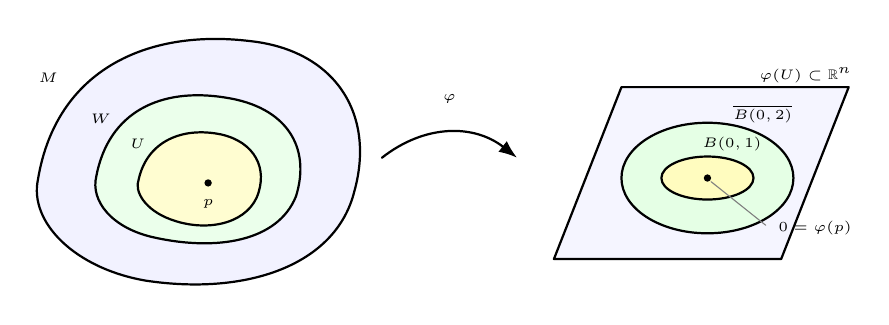
\begin{tikzpicture}[
    >=Latex,
    font=\small,
    line cap=round,
    line join=round,
    scale=0.78
]

% M
\draw[
    thick,
    fill=blue!5
]
    (-5.4,0.1)
    .. controls (-5.1,1.9) and (-3.6,2.55) .. (-1.95,2.35)
    .. controls (-0.55,2.2) and (0.10,1.15) .. (-0.25,-0.10)
    .. controls (-0.55,-1.30) and (-2.0,-1.80) .. (-3.65,-1.55)
    .. controls (-4.8,-1.35) and (-5.55,-0.60) .. (-5.4,0.1);

\node[anchor=west, font=\tiny] at (-5.55,1.75)
    {$M$};

% W
\draw[
    thick,
    fill=green!8
]
    (-4.45,0.15)
    .. controls (-4.25,1.20) and (-3.40,1.60) .. (-2.35,1.43)
    .. controls (-1.35,1.28) and (-0.95,0.62) .. (-1.20,-0.18)
    .. controls (-1.50,-0.92) and (-2.50,-1.07) .. (-3.50,-0.85)
    .. controls (-4.20,-0.70) and (-4.55,-0.25) .. (-4.45,0.15);

\node[anchor=west, font=\tiny] at (-4.70,1.08)
    {$W$};

% U
\draw[
    thick,
    fill=yellow!18
]
    (-3.76,0.10)
    .. controls (-3.62,0.72) and (-3.05,0.96) .. (-2.42,0.83)
    .. controls (-1.88,0.71) and (-1.64,0.28) .. (-1.84,-0.20)
    .. controls (-2.05,-0.65) and (-2.70,-0.76) .. (-3.25,-0.55)
    .. controls (-3.65,-0.40) and (-3.84,-0.10) .. (-3.76,0.10);

\node[anchor=west, font=\tiny] at (-4.05,0.67)
    {$U$};

% Punkt p
\fill (-2.63,0.04) circle (1.7pt);

\node[below=5pt, font=\tiny] at (-2.63,0.15)
    {$p$};

% Strzałka \varphi
\draw[->,thick]
    (0.20,0.45)
    .. controls (0.90,1.00) and (1.70,1.00) ..
    (2.40,0.45);

\node[above=5pt, font=\tiny] at (1.30,0.95)
    {$\varphi$};

% Obraz mapy
\draw[
    thick,
    fill=blue!4
]
    (3.0,-1.2)
    --
    (4.1,1.6)
    --
    (7.8,1.6)
    --
    (6.7,-1.2)
    --
    cycle;

\node[above=7pt, font=\tiny] at (7.10,1.20)
    {$\varphi(U)\subset\mathbb{R}^n$};

% \overline{B(0,2)}
\draw[
    thick,
    fill=green!10
]
    (5.50,0.12)
    ellipse (1.40 and 0.9);

\node[above=8pt, font=\tiny] at (6.40,0.5)
    {$\overline{B(0,2)}$};

% B(0,1)
\draw[
    thick,
    fill=yellow!25
]
    (5.50,0.12)
    ellipse (0.75 and 0.35);

\node[below=7pt, font=\tiny] at (5.90, 1.26)
    {$B(0,1)$};

% 0 = \varphi(p)
\fill (5.50,0.12) circle (1.7pt);

\draw[thin,gray] (5.56,0.06) -- (6.45,-0.65);
\node[anchor=west, font=\tiny] at (6.50,-0.70)
    {$0=\varphi(p)$};

\end{tikzpicture}

\caption{
Wybór mapy $(U,\varphi)$ wokół punktu $p$:
$U\subseteq W$, $\varphi(p)=0$ oraz
$\overline{B(0,2)}\subseteq\varphi(U)$.
}
\label{fig:kapelusz-mapa}

\end{figure}


% ============================================================
% RYSUNEK 2
% Wykres funkcji kapelusz
% ============================================================

\begin{figure}[ht]
\centering

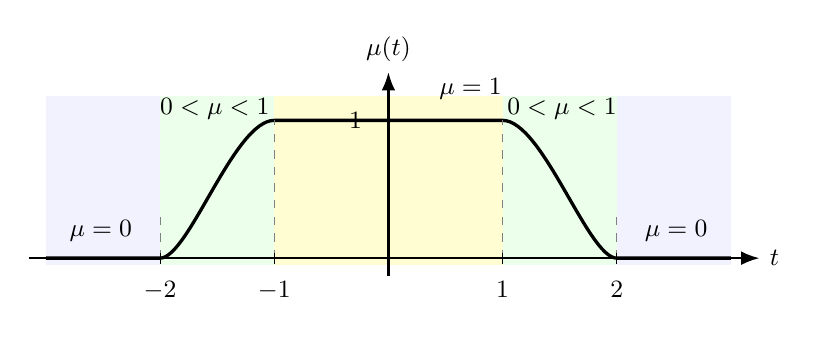
\begin{tikzpicture}[
    >=Latex,
    font=\small,
    x=1.45cm,
    y=1.75cm
]

% Delikatne kolorowe obszary
\fill[blue!5]
    (-3,-0.05)
    rectangle
    (-2,1.18);

\fill[green!8]
    (-2,-0.05)
    rectangle
    (-1,1.18);

\fill[yellow!18]
    (-1,-0.05)
    rectangle
    (1,1.18);

\fill[green!8]
    (1,-0.05)
    rectangle
    (2,1.18);

\fill[blue!5]
    (2,-0.05)
    rectangle
    (3,1.18);

% Oś pozioma
\draw[->,thick]
    (-3.15,0)
    --
    (3.25,0)
    node[right] {$t$};

% Oś pionowa
\draw[->,thick]
    (0,-0.13)
    --
    (0,1.35)
    node[above] {$\mu(t)$};

% Wykres funkcji kapelusz
\draw[very thick]
    (-3,0)
    --
    (-2,0)
    .. controls (-1.75,0) and (-1.35,1) ..
    (-1,1)
    --
    (1,1)
    .. controls (1.35,1) and (1.75,0) ..
    (2,0)
    --
    (3,0);

% Linie pomocnicze
\draw[dashed,gray]
    (-1,0) -- (-1,1);

\draw[dashed,gray]
    (1,0) -- (1,1);

\draw[dashed,gray]
    (-2,0) -- (-2,0.36);

\draw[dashed,gray]
    (2,0) -- (2,0.36);

% Znaczniki na osi
\draw
    (-2,0.04) -- (-2,-0.04);
\node[below=5pt] at (-2,0)
    {$-2$};

\draw
    (-1,0.04) -- (-1,-0.04);
\node[below=5pt] at (-1,0)
    {$-1$};

\draw
    (1,0.04) -- (1,-0.04);
\node[below=5pt] at (1,0)
    {$1$};

\draw
    (2,0.04) -- (2,-0.04);
\node[below=5pt] at (2,0)
    {$2$};

% Poziom 1
\draw
    (-0.04,1) -- (0.04,1);

\node[left=6pt] at (0,1)
    {$1$};

% Opisy — odsunięte od wykresu
\node[above=4pt] at (0.72,1)
    {$\mu=1$};

\node at (-1.52,1.08)
    {$0<\mu<1$};

\node at (1.52,1.08)
    {$0<\mu<1$};

\node at (-2.52,0.20)
    {$\mu=0$};

\node at (2.52,0.20)
    {$\mu=0$};

\end{tikzpicture}

\caption{
Jednowymiarowy przekrój funkcji odcinającej $\mu$.
Funkcja jest równa $1$ dla $|t|\leq1$,
płynnie maleje dla $1<|t|<2$
i znika dla $|t|\geq2$.
}
\label{fig:kapelusz-wykres}

\end{figure}




\begin{lemat}[Lokalność derywacji]\label{lem:lokalnosc}
Niech $v\in T_p^CM$ będzie derywacją w $p$. Jeśli $h\in C^\infty(M)$ znika na pewnym
otoczeniu punktu $p$, to $v(h)=0$. W szczególności, jeśli $f,g\in C^\infty(M)$ pokrywają
się na pewnym otoczeniu $p$, to $v(f)=v(g)$; wartość $v(f)$ zależy więc jedynie od
zachowania $f$ w dowolnie małym otoczeniu $p$.
\end{lemat}
\begin{proof}
Z reguły Leibniza zastosowanej do $f=g=\mathbf1$ (funkcji stałej równej $1$),
$v(\mathbf1)=v(\mathbf1\cdot\mathbf1)=2v(\mathbf1)$, skąd $v(\mathbf1)=0$; z liniowości,
$v(c)=0$ dla każdej funkcji stałej $c$.

Niech $h\equiv0$ na otoczeniu otwartym $W\ni p$. Wybierzmy mapę $(U,\varphi)$ wokół $p$ z
$U\subseteq W$, $\varphi(p)=0$, oraz (po przeskalowaniu)
$\overline{B(0,2)}\subseteq\varphi(U)$.
Zdefiniujmy $\tilde\mu\colon M\to\R$: $\tilde\mu(q):=\mu(\varphi(q))$ dla $q\in U$, oraz
$\tilde\mu(q):=0$ dla $q\notin U$. Nośnik jest zawarty w zwartym
zbiorze $K=\varphi^{-1}(\overline{B(0,2)})\subset U$.
Ponieważ $M$ jest Hausdorffa, $K$ jest domknięty w $M$.
Na otwartym pokryciu $U, M\setminus K$ obie gładkie definicje
pokrywają się, więc $\tilde\mu\in C^\infty(M)$, równa $1$ na otoczeniu $p$ i znikająca poza
$U\subseteq W$. Wówczas $\tilde\mu\cdot h\equiv0$ na całym $M$, więc $v(\tilde\mu h)=0$.
Z reguły Leibniza, $0=v(\tilde\mu h)=\tilde\mu(p)v(h)+h(p)v(\tilde\mu)=v(h)$ (bo
$\tilde\mu(p)=1$, $h(p)=0$). Zatem $v(h)=0$. Ostatnia część lematu wynika z zastosowania
powyższego do $h:=f-g$.
\end{proof}

\begin{twierdzenie}\label{tw:baza-styczna}
Niech $(U,\varphi)$ będzie mapą dopuszczalną wokół $p$,
$\varphi=(x^1,\dots,x^n)$,
gdzie $x^i=\pi_i\circ\varphi\colon U\to\R$ są funkcjami współrzędnymi,
czyli dla każdego $q\in U$ zachodzi
$\varphi(q)=\bigl(x^1(q),\dots,x^n(q)\bigr)$,
oraz załóżmy, że $\varphi(p)=0$. Wówczas:
\begin{enumerate}[label=(\alph*)]
\item Odwzorowanie $\Phi\colon T_p^AM\to T_p^CM$ jest izomorfizmem liniowym.
\item Elementy $\frac{\partial}{\partial x^1}\big|_p,\dots,\frac{\partial}{\partial x^n}
\big|_p\in T_p^CM$, zdefiniowane przez $\frac{\partial}{\partial x^i}\big|_p(f):=
\frac{\partial(f\circ\varphi^{-1})}{\partial x^i}(\varphi(p))$, stanowią bazę $T_p^CM$.
W szczególności $\dim T_pM=n$.
\end{enumerate}
\end{twierdzenie}

\begin{proof}
\emph{(a), injektywność.} Załóżmy $\Phi([\gamma])=0$, tzn.\ $(f\circ\gamma)'(0)=0$ dla
wszystkich $f\in C^\infty(M)$. Wybierzmy funkcję odcinającą
$\tilde\mu$ o zwartym nośniku zawartym w $U$, równą $1$ blisko $p$,
jak w dowodzie Lematu~\ref{lem:lokalnosc}.
Dla $i=1,\dots,n$ niech $\tilde x^i:=\tilde\mu\,x^i
=\tilde\mu\,\varphi^i$ na $U$ (rozszerzone przez $0$ poza $U$) —
funkcja gładka na $M$, pokrywająca się z $\varphi^i$ na otoczeniu $p$. Z założenia,
$0=\Phi([\gamma])(\tilde x^i)=(\tilde x^i\circ\gamma)'(0)$; blisko $t=0$, $\gamma(t)\in U$
i tam $\tilde x^i\circ\gamma=\varphi^i\circ\gamma$, więc $(\varphi^i\circ\gamma)'(0)=0$ dla
każdego $i$, czyli $(\varphi\circ\gamma)'(0)=0\in\R^n$. Oznacza to $\gamma\sim
\gamma_{\text{stała}}$ (gdzie $\gamma_{\text{stała}}(t)\equiv p$), czyli $[\gamma]=0$ w
$T_p^AM$. Zatem $\ker\Phi=\{0\}$.

\emph{(a), surjektywność — Lemat Hadamarda.} Niech $v\in T_p^CM$. Bez straty ogólności
$\varphi(U)$ jest kulą (gwiaździstą względem $0$). Niech $\tilde f:=f\circ\varphi^{-1}\in
C^\infty(\varphi(U))$; z Lematu~\ref{lem:hadamard} istnieją $g_1,\dots,g_n$ z
\[
\tilde f(x)=\tilde f(0)+\sum_ix^ig_i(x), \qquad g_i(0)=\frac{\partial\tilde f}{\partial x^i}
(0)=\frac{\partial}{\partial x^i}\Big|_p(f).
\]
Podstawiając $x=\varphi(q)$: $f(q)=f(p)+\sum_i\varphi^i(q)\,g_i(\varphi(q))$ dla $q$
blisko $p$. Niech $\widetilde{\varphi^i}$, $\tilde g_i$ oznaczają (jak wyżej) rozszerzenia
$\varphi^i$ oraz $g_i\circ\varphi$ do funkcji gładkich na $M$, pokrywające się z
oryginałami na otoczeniu $p$. Funkcja $F:=f(p)\cdot\mathbf1+\sum_i\widetilde{\varphi^i}\,
\tilde g_i$ pokrywa się z $f$ na otoczeniu $p$, więc $v(f)=v(F)$ (Lemat~\ref{lem:lokalnosc}).
Z liniowości $v$, reguły Leibniza (korzystając z $\widetilde{\varphi^i}(p)=0$,
$v(\mathbf1)=0$):
\[
v(f)=v(F)=\sum_i\Big(\widetilde{\varphi^i}(p)\,v(\tilde g_i)+\tilde g_i(p)\,v
(\widetilde{\varphi^i})\Big)=\sum_ig_i(0)\,v(\widetilde{\varphi^i})=\sum_{i=1}^n
v(\widetilde{\varphi^i})\cdot\frac{\partial}{\partial x^i}\Big|_p(f).
\]
Kładąc $c_i:=v(\widetilde{\varphi^i})\in\R$, mamy $v=\sum_ic_i\,\frac{\partial}{\partial
x^i}\big|_p$ jako funkcjonały. Niech $\gamma(t):=\varphi^{-1}(t\cdot(c_1,\dots,c_n))$; wtedy
$\Phi([\gamma])(f)=(f\circ\gamma)'(0)=D(f\circ\varphi^{-1})(0)\cdot(c_1,\dots,c_n)=
\sum_ic_i\frac{\partial}{\partial x^i}\big|_p(f)=v(f)$ dla każdego $f$, czyli
$\Phi([\gamma])=v$. To dowodzi surjektywności, a wraz z liniowością i injektywnością —
części (a).

\emph{(b).} Powyższy rachunek pokazał, że każdy $v\in T_p^CM$ jest kombinacją liniową
$\sum_ic_i\frac{\partial}{\partial x^i}\big|_p$ — więc baza ta rozpina $T_p^CM$. Niezależność
liniowa: załóżmy $\sum_ic_i\frac{\partial}{\partial x^i}\big|_p=0$. Stosując obie strony
do $\widetilde{\varphi^j}$ i korzystając z $\frac{\partial}{\partial x^i}\big|_p
(\widetilde{\varphi^j})=\frac{\partial x^j}{\partial x^i}(0)=\delta_i^j$, otrzymujemy
$0=\sum_ic_i\delta_i^j=c_j$ dla każdego $j$. Zatem $\{\partial/\partial x^i|_p\}$ jest
bazą $T_p^CM$; w szczególności $\dim T_p^CM=n$.
\end{proof}

\begin{wniosek}
Definicje A, B i C przestrzeni stycznej są kanonicznie izomorficzne. Piszemy odtąd po
prostu $T_pM$ i mówimy o \emph{przestrzeni stycznej do $M$ w punkcie $p$} — jest to
$n$-wymiarowa przestrzeń wektorowa. W mapie $(U,\varphi)$, gdzie $\varphi=(x^1,\dots,x^n)$,
jej \emph{bazą współrzędnościową} są wektory
\[
\left.\frac{\partial}{\partial x^1}\right|_p,\ \dots,\
\left.\frac{\partial}{\partial x^n}\right|_p.
\]
\end{wniosek}

\begin{figure}[ht]
\centering
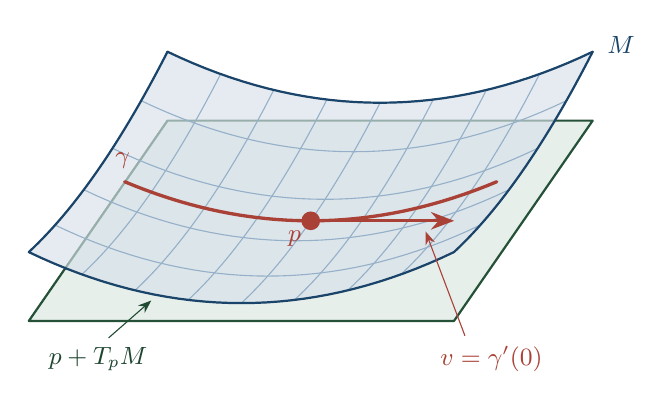
\begin{tikzpicture}[>=Stealth,scale=1.35,line cap=round,line join=round]
% S(u,v)=(u,v,.12u^2+.08v^2), rzut (x,y,z)->(x+.45y,.65y+z).
% Brzeg wypełnienia, siatka i krzywa używają tej samej parametryzacji.
\filldraw[fill=manifoldgreen!12,draw=manifoldgreen!65!black,thick]
 (-2.6525,-.9425)--(1.3475,-.9425)--(2.6525,.9425)--(-1.3475,.9425)--cycle;
\path[fill=manifoldblue!18,opacity=.65]
 (-2.65250,-0.29430)
  --(-2.48583,-0.37097)
  --(-2.31917,-0.44097)
  --(-2.15250,-0.50430)
  --(-1.98583,-0.56097)
  --(-1.81917,-0.61097)
  --(-1.65250,-0.65430)
  --(-1.48583,-0.69097)
  --(-1.31917,-0.72097)
  --(-1.15250,-0.74430)
  --(-0.98583,-0.76097)
  --(-0.81917,-0.77097)
  --(-0.65250,-0.77430)
  --(-0.48583,-0.77097)
  --(-0.31917,-0.76097)
  --(-0.15250,-0.74430)
  --(0.01417,-0.72097)
  --(0.18083,-0.69097)
  --(0.34750,-0.65430)
  --(0.51417,-0.61097)
  --(0.68083,-0.56097)
  --(0.84750,-0.50430)
  --(1.01417,-0.44097)
  --(1.18083,-0.37097)
  --(1.34750,-0.29430)
  --(1.40187,-0.24262)
  --(1.45625,-0.18861)
  --(1.51063,-0.13226)
  --(1.56500,-0.07358)
  --(1.61938,-0.01256)
  --(1.67375,0.05080)
  --(1.72812,0.11649)
  --(1.78250,0.18452)
  --(1.83688,0.25489)
  --(1.89125,0.32759)
  --(1.94562,0.40263)
  --(2.00000,0.48000)
  --(2.05437,0.55971)
  --(2.10875,0.64176)
  --(2.16312,0.72614)
  --(2.21750,0.81286)
  --(2.27188,0.90191)
  --(2.32625,0.99330)
  --(2.38063,1.08703)
  --(2.43500,1.18309)
  --(2.48937,1.28149)
  --(2.54375,1.38222)
  --(2.59813,1.48529)
  --(2.65250,1.59070)
  --(2.48583,1.51403)
  --(2.31917,1.44403)
  --(2.15250,1.38070)
  --(1.98583,1.32403)
  --(1.81917,1.27403)
  --(1.65250,1.23070)
  --(1.48583,1.19403)
  --(1.31917,1.16403)
  --(1.15250,1.14070)
  --(0.98583,1.12403)
  --(0.81917,1.11403)
  --(0.65250,1.11070)
  --(0.48583,1.11403)
  --(0.31917,1.12403)
  --(0.15250,1.14070)
  --(-0.01417,1.16403)
  --(-0.18083,1.19403)
  --(-0.34750,1.23070)
  --(-0.51417,1.27403)
  --(-0.68083,1.32403)
  --(-0.84750,1.38070)
  --(-1.01417,1.44403)
  --(-1.18083,1.51403)
  --(-1.34750,1.59070)
  --(-1.40187,1.48529)
  --(-1.45625,1.38222)
  --(-1.51063,1.28149)
  --(-1.56500,1.18309)
  --(-1.61938,1.08703)
  --(-1.67375,0.99330)
  --(-1.72812,0.90191)
  --(-1.78250,0.81286)
  --(-1.83688,0.72614)
  --(-1.89125,0.64176)
  --(-1.94562,0.55971)
  --(-2.00000,0.48000)
  --(-2.05437,0.40263)
  --(-2.10875,0.32759)
  --(-2.16312,0.25489)
  --(-2.21750,0.18452)
  --(-2.27188,0.11649)
  --(-2.32625,0.05080)
  --(-2.38063,-0.01256)
  --(-2.43500,-0.07358)
  --(-2.48937,-0.13226)
  --(-2.54375,-0.18861)
  --(-2.59813,-0.24262) --cycle;
\foreach \vv in {-1.45,-.9,-.3,.3,.9,1.45}{
 \draw[manifoldblue!48,thin] plot[domain=-2:2,samples=35]
  ({\x+.45*\vv},{.65*\vv+.12*\x*\x+.08*\vv*\vv});}
\foreach \uu in {-2,-1.5,-1,-.5,0,.5,1,1.5,2}{
 \draw[manifoldblue!48,thin] plot[domain=-1.45:1.45,samples=30]
  ({\uu+.45*\x},{.65*\x+.12*\uu*\uu+.08*\x*\x});}
\foreach \vv in {-1.45,1.45}{
 \draw[manifoldblue!75!black,thick] plot[domain=-2:2,samples=35]
  ({\x+.45*\vv},{.65*\vv+.12*\x*\x+.08*\vv*\vv});}
\foreach \uu in {-2,2}{
 \draw[manifoldblue!75!black,thick] plot[domain=-1.45:1.45,samples=30]
  ({\uu+.45*\x},{.65*\x+.12*\uu*\uu+.08*\x*\x});}
\draw[manifoldred,very thick] plot[domain=-1.75:1.75,samples=40]
 ({\x},{.12*\x*\x});
\fill[manifoldred] (0,0) circle (2.5pt) node[below left,font=\small] {$p$};
\draw[->,very thick,manifoldred] (0,0)--(1.35,0);
\node[font=\small,manifoldred] at (-1.77,.57) {$\gamma$};
\node[font=\small\bfseries,manifoldblue!75!black] at (2.92,1.65) {$M$};
\node[font=\small,manifoldgreen!55!black] at (-2.0,-1.30) {$p+T_pM$};
\draw[->,manifoldgreen!60!black,thin] (-1.9,-1.10)--(-1.5,-.75);
\node[font=\small,manifoldred] at (1.7,-1.30) {$v=\gamma'(0)$};
\draw[->,manifoldred,thin] (1.45,-1.08)--(1.08,-.10);
\end{tikzpicture}
\caption{Przestrzeń styczna: zielony równoległobok przedstawia afiniczną
płaszczyznę $p+T_pM$ przy zanurzonej powierzchni $M$. Czerwona krzywa
$\gamma$ leży na $M$, a wektor $v=\gamma'(0)$ leży w płaszczyźnie stycznej.
Siatka powierzchni odchyla się od tej płaszczyzny poza punktem $p$.}
\label{fig:tangent}
\end{figure}


\subsection*{Zmiana współrzędnych wektora stycznego}

\begin{fakt}
Niech $(U,\varphi)$ i $(V,\psi)$ będą mapami wokół $p\in M$, a
$[\gamma]\in T_pM$, gdzie $\gamma:(-\varepsilon,\varepsilon)\to M, \ \gamma(0)=p$.
Współrzędne wektora $[\gamma]$ w mapie $\varphi$ są dane przez $[\gamma]_{\varphi}:=(\varphi\circ\gamma)'(0)\in\R^n$,
a w mapie $\psi$ przez $[\gamma]_{\psi}:=(\psi\circ\gamma)'(0)$.
Wtedy
\[
\boxed{
[\gamma]_{\psi}
=
D(\psi\circ\varphi^{-1})(\varphi(p))\,[\gamma]_{\varphi}.
}
\]
\end{fakt}

\begin{proof}
Ponieważ $\psi\circ\gamma = (\psi\circ\varphi^{-1})\circ(\varphi\circ\gamma)$,
z reguły łańcuchowej otrzymujemy
\[
(\psi\circ\gamma)'(0)
=
D(\psi\circ\varphi^{-1})(\varphi(p))
\,(\varphi\circ\gamma)'(0),
\]
czyli dokładnie
\[
[\gamma]_{\psi}
=
D(\psi\circ\varphi^{-1})(\varphi(p))\,[\gamma]_{\varphi}.
\]
\end{proof}
Jak pokaże następna sekcja, jedną z najbardziej użytecznych definicji
przestrzeni stycznej jest konstrukcja za pomocą derywacji.
Podamy zatem regułę transformacji wektorów stycznych również
w tym ujęciu.

\begin{fakt}[Transformacja derywacji współrzędnych]
\label{fakt:transformacja-derywacji}
Niech $(U,\varphi)$ i $(V,\psi)$ będą mapami rozmaitości
$M$ wokół punktu $p\in U\cap V$, przy czym $\varphi=(x^1,\ldots,x^n), \ \psi=(y^1,\ldots,y^n)$.
Niech
\[
\left\{
\left.\frac{\partial}{\partial x^i}\right|_p
\right\}_{i=1}^n,
\qquad
\left\{
\left.\frac{\partial}{\partial y^j}\right|_p
\right\}_{j=1}^n
\]
oznaczają odpowiadające tym mapom bazy przestrzeni
stycznej $T_pM$, zdefiniowane za pomocą derywacji.

Wówczas zachodzi \emph{reguła transformacji derywacji
współrzędnych}:
\begin{equation}
\label{eq:transformacja-derywacji}
\boxed{
\left.\frac{\partial}{\partial x^i}\right|_p
=
\sum_{j=1}^n
\frac{\partial y^j}{\partial x^i}(p)
\left.\frac{\partial}{\partial y^j}\right|_p,
\qquad i=1,\ldots,n,
}
\end{equation}
gdzie
\[
\frac{\partial y^j}{\partial x^i}(p)
:=
\left.
\frac{\partial(y^j\circ\varphi^{-1})}{\partial u^i}
\right|_{u=\varphi(p)},
\]
a $u^1,\ldots,u^n$ oznaczają standardowe współrzędne
w $\R^n$.

Współczynniki te są elementami macierzy Jacobiego
odwzorowania przejścia:
\[
\boxed{
J_{\psi\varphi}(p)
:=
D(\psi\circ\varphi^{-1})(\varphi(p))
=
\left[
\frac{\partial y^j}{\partial x^i}(p)
\right]_{j,i=1}^n.
}
\]
\end{fakt}

\begin{proof}
Przypomnijmy, że dla dowolnej funkcji $f$ gładkiej
w otoczeniu punktu $p$ derywacje współrzędnych
są określone wzorami
\[
\left.\frac{\partial}{\partial x^i}\right|_p(f)
=
\left.
\frac{\partial(f\circ\varphi^{-1})}{\partial u^i}
\right|_{u=\varphi(p)}
\]
oraz
\[
\left.\frac{\partial}{\partial y^j}\right|_p(f)
=
\left.
\frac{\partial(f\circ\psi^{-1})}{\partial v^j}
\right|_{v=\psi(p)},
\]
gdzie $u^i$ i $v^j$ są standardowymi współrzędnymi
w $\R^n$.

Rozważmy odwzorowanie przejścia
\[
F:=\psi\circ\varphi^{-1}
\colon
\varphi(U\cap V)\longrightarrow\psi(U\cap V).
\]
Ponieważ $\psi=(y^1,\ldots,y^n)$,
jego funkcje współrzędne mają postać $F^j=y^j\circ\varphi^{-1}, \ j=1,\ldots,n$.
W szczególności, przy oznaczeniach $u:=\varphi(p), \ v:=\psi(p)=F(u)$,
otrzymujemy
\[
DF(u)
=
\left[
\frac{\partial F^j}{\partial u^i}(u)
\right]_{j,i=1}^n
=
\left[
\frac{\partial y^j}{\partial x^i}(p)
\right]_{j,i=1}^n
=
J_{\psi\varphi}(p).
\]

Zauważmy teraz, że w otoczeniu punktu $u$
możemy wstawić identyczność
$\psi^{-1}\circ\psi$ i zapisać
\[
f\circ\varphi^{-1}
=f\circ\psi^{-1}\circ\psi\circ\varphi^{-1}
=(f\circ\psi^{-1})\circ(\psi\circ\varphi^{-1})
=(f\circ\psi^{-1})\circ F.
\]

Stosując regułę łańcuchową, otrzymujemy
\[
\boxed{
D(f\circ\varphi^{-1})(u)
=
D(f\circ\psi^{-1})(v)\,DF(u).
}
\]

Rozpiszmy tę równość w postaci macierzowej:
\[
\begin{gathered}
\underbrace{
\begin{pmatrix}
\displaystyle
\frac{\partial(f\circ\varphi^{-1})}{\partial u^1}(u)
&
\cdots
&
\displaystyle
\frac{\partial(f\circ\varphi^{-1})}{\partial u^n}(u)
\end{pmatrix}
}_{1\times n}
\\[1mm]
=
\underbrace{
\begin{pmatrix}
\displaystyle
\frac{\partial(f\circ\psi^{-1})}{\partial v^1}(v)
&
\cdots
&
\displaystyle
\frac{\partial(f\circ\psi^{-1})}{\partial v^n}(v)
\end{pmatrix}
}_{1\times n}
\underbrace{
\begin{pmatrix}
\displaystyle\frac{\partial y^1}{\partial x^1}
&\cdots&
\displaystyle\frac{\partial y^1}{\partial x^n}
\\[2mm]
\vdots&\ddots&\vdots
\\[2mm]
\displaystyle\frac{\partial y^n}{\partial x^1}
&\cdots&
\displaystyle\frac{\partial y^n}{\partial x^n}
\end{pmatrix}_{\!p}
}_{n\times n}.
\end{gathered}
\]

Korzystając z definicji derywacji współrzędnych,
możemy tę samą równość zapisać krócej:
\[
\begin{pmatrix}
\displaystyle
\left.\frac{\partial}{\partial x^1}\right|_p(f)
&
\cdots
&
\displaystyle
\left.\frac{\partial}{\partial x^n}\right|_p(f)
\end{pmatrix}
=
\begin{pmatrix}
\displaystyle
\left.\frac{\partial}{\partial y^1}\right|_p(f)
&
\cdots
&
\displaystyle
\left.\frac{\partial}{\partial y^n}\right|_p(f)
\end{pmatrix}
J_{\psi\varphi}(p).
\]

Porównując $i$-te współrzędne obu stron,
dostajemy
\[
\left.\frac{\partial}{\partial x^i}\right|_p(f)
=
\sum_{j=1}^n
\frac{\partial y^j}{\partial x^i}(p)
\left.\frac{\partial}{\partial y^j}\right|_p(f).
\]

Ponieważ równość ta zachodzi dla każdej funkcji
$f$ gładkiej w otoczeniu $p$, obie strony
wyznaczają tę samą derywację w punkcie $p$.
Otrzymujemy zatem wzór
\eqref{eq:transformacja-derywacji}.
\end{proof}

Zauważmy, że macierz Jacobiego $J_{\psi\varphi}(p) = D(\psi\circ\varphi^{-1})(\varphi(p))$
jest dokładnie macierzą współczynników występujących
w regule transformacji derywacji
\eqref{eq:transformacja-derywacji}.
W zapisie macierzowym reguła ta przyjmuje postać
\[
\boxed{
\begin{pmatrix}
\displaystyle\left.\frac{\partial}{\partial x^1}\right|_p
&
\cdots
&
\displaystyle\left.\frac{\partial}{\partial x^n}\right|_p
\end{pmatrix}
=
\begin{pmatrix}
\displaystyle\left.\frac{\partial}{\partial y^1}\right|_p
&
\cdots
&
\displaystyle\left.\frac{\partial}{\partial y^n}\right|_p
\end{pmatrix}
J_{\psi\varphi}(p).
}
\]

W szczególności, jeżeli wektor styczny $X\in T_pM$
ma w obu bazach przedstawienia
\[
X=
\sum_{i=1}^n X_\varphi^i
\left.\frac{\partial}{\partial x^i}\right|_p
=
\sum_{j=1}^n X_\psi^j
\left.\frac{\partial}{\partial y^j}\right|_p,
\]
to jego kolumny współrzędnych spełniają
\[
\boxed{
\begin{pmatrix}
X_\psi^1\\
\vdots\\
X_\psi^n
\end{pmatrix}
=
D(\psi\circ\varphi^{-1})(\varphi(p))
\begin{pmatrix}
X_\varphi^1\\
\vdots\\
X_\varphi^n
\end{pmatrix}.
}
\]

Zatem różniczka odwzorowania przejścia
$\psi\circ\varphi^{-1}$ opisuje zarówno
transformację baz przestrzeni stycznej,
jak i transformację współrzędnych wektorów stycznych.

\begin{przyklad}[Zmiana współrzędnych wektora stycznego na $\mathbb{RP}^2$]
\label{prz:RP2-styczna-1}
Wróćmy do map z przykładu~\ref{prz:RP2-przejscie-1}:
punkt $[1:u:v]$, gdzie $u\ne0$, ma w drugiej mapie współrzędne
$(a,b)=(1/u,v/u)$. Zastosujemy do tego przejścia właśnie udowodnioną
regułę zmiany współrzędnych wektora stycznego.

Odwzorowanie $\varphi_1\circ\varphi_0^{-1}$ opisuje zmianę
\emph{współrzędnych punktów} rozmaitości. Jego różniczka opisuje natomiast
odpowiadającą jej zmianę \emph{współrzędnych wektorów stycznych}.

Niech $p\in U_0\cap U_1$ oraz $\varphi_0(p)=(u,v)$.
Mapy $\varphi_0$ i $\varphi_1$ wyznaczają dwie bazy przestrzeni stycznej
$T_p\mathbb{RP}^2$:
\[
\left\{
\left.\frac{\partial}{\partial u}\right|_p,
\left.\frac{\partial}{\partial v}\right|_p
\right\},
\qquad
\left\{
\left.\frac{\partial}{\partial a}\right|_p,
\left.\frac{\partial}{\partial b}\right|_p
\right\}.
\]
Jeżeli wektor $X\in T_p\mathbb{RP}^2$ ma w bazie indukowanej przez
$\varphi_0$ współrzędne
\[
X
=
\dot u\left.\frac{\partial}{\partial u}\right|_p
+
\dot v\left.\frac{\partial}{\partial v}\right|_p,
\]
to jego współrzędne w bazie indukowanej przez $\varphi_1$ otrzymujemy,
stosując różniczkę odwzorowania przejścia:
\[
\begin{pmatrix}
\dot a\\[1mm]
\dot b
\end{pmatrix}
=
D(\varphi_1\circ\varphi_0^{-1})(u,v)
\begin{pmatrix}
\dot u\\[1mm]
\dot v
\end{pmatrix}.
\]
A zatem
\[
\dot a=-\frac{\dot u}{u^2},
\qquad
\dot b
=
-\frac{v\dot u}{u^2}
+
\frac{\dot v}{u}.
\]
Ten sam wektor styczny możemy więc zapisać jako
\[
X
=
\dot u\left.\frac{\partial}{\partial u}\right|_p
+
\dot v\left.\frac{\partial}{\partial v}\right|_p
=
\dot a\left.\frac{\partial}{\partial a}\right|_p
+
\dot b\left.\frac{\partial}{\partial b}\right|_p.
\]

Innymi słowy, odwzorowanie przejścia
$\varphi_1\circ\varphi_0^{-1}$ zmienia współrzędne punktu na rozmaitości,
natomiast jego różniczka $d(\varphi_1\circ\varphi_0^{-1})_{\varphi_0(p)}$
zmienia reprezentację współrzędnościową tego samego wektora
$X\in T_p\mathbb{RP}^2$ względem baz przestrzeni stycznej indukowanych
przez obie mapy.
\end{przyklad}

\subsection*{Przestrzeń styczna w punkcie brzegu}

Niech teraz $p\in\partial M$. \emph{Kiełek}\index{kielek funkcji@Kiełek funkcji} funkcji gładkiej w $p$
to jej klasa względem równości w pewnym otoczeniu punktu $p$
otwartym w $M$;
funkcje są tu gładkie w sensie przedłużalności z półprzestrzeni.
Ich algebra to $C^\infty_p(M)$. Definiujemy $T_pM$ jako przestrzeń
$\R$-liniowych derywacji $D:C^\infty_p(M)\to\R$ spełniających $D(fg)=f(p)D(g)+g(p)D(f)$.
Wartość kiełka w $p$ jest dobrze określona. To lokalna wersja
Definicji C, która nie wymaga krzywej przechodzącej przez $p$
w obu kierunkach czasu.

Użycie kiełków jest tutaj istotne. Gładkie przedłużenie funkcji
$f$ poza brzeg, do otoczenia $\varphi(p)$ w $\R^n$, nie jest
jednoznaczne i stanowi jedynie pomocnicze narzędzie służące do
zdefiniowania gładkości. Przestrzeń styczna powinna natomiast zależeć
wyłącznie od lokalnego zachowania funkcji na samej rozmaitości $M$,
a nie od arbitralnego wyboru jej wartości poza $M$.

Dokładniej, dwa różne gładkie przedłużenia
$\widetilde f_1,\widetilde f_2$ mogą być różnymi funkcjami na
otoczeniu $\varphi(p)$ w $\R^n$, mimo że ich ograniczenia do
$\mathbb H^n$ wyznaczają tę samą funkcję na $M$. Nie chcemy więc
traktować samych przedłużeń jako obiektów, na których działa derywacja.
Obiektem właściwym jest kiełek funkcji na $M$, natomiast przedłużenie
wybieramy dopiero wtedy, gdy chcemy wykonać rachunek we współrzędnych.

Co więcej, derywacja w punkcie $p$ jest obiektem lokalnym: jej wartość
na funkcji zależy jedynie od zachowania tej funkcji w dowolnie małym
otoczeniu $p$. Dlatego naturalną dziedziną derywacji jest algebra
kiełków $C^\infty_p(M)$.

\begin{stwierdzenie}[Pełny wymiar przestrzeni stycznej przy brzegu]
\label{prop:styczna-brzeg-1}
W mapie półprzestrzennej $\varphi$ z $\varphi(p)=0$ każda taka
derywacja ma jednoznaczną postać
\[
D(f)=\sum_{i=1}^n v^i\partial_i\widetilde f(0),
\qquad v\in\R^n,
\]
gdzie $\widetilde f$ jest dowolnym gładkim przedłużeniem
$f\circ\varphi^{-1}$ na otoczenie zera w $\R^n$.
Wzór nie zależy od wyboru przedłużenia. Przy zmianie mapy współrzędne
$v$ zmieniają się przez odwracalną macierz Jacobiego przejścia.
W szczególności $\dim T_pM=n$, a inkluzja brzegu identyfikuje
$T_p\partial M$ z podprzestrzenią $v^n=0$.
\end{stwierdzenie}

\begin{proof}
Najpierw sprawdźmy, że prawa strona wzoru nie zależy od wyboru
przedłużenia $\widetilde f$. Jeżeli $\widetilde f_1$ i
$\widetilde f_2$ są dwoma gładkimi przedłużeniami reprezentującymi
ten sam kiełek funkcji $f\circ\varphi^{-1}$, to ich różnica znika
na pewnej małej półkuli $B_\varepsilon(0)\cap\mathbb H^n$.
Na jej części wewnętrznej, gdzie $x^n>0$, znikają więc wszystkie
pierwsze pochodne tej różnicy, a przez ciągłość znikają one również
w punkcie $0$. W konsekwencji
\[
\partial_i\widetilde f_1(0)
=
\partial_i\widetilde f_2(0),
\qquad i=1,\ldots,n.
\]
Zatem dla każdego $v\in\R^n$ wzór
\[
D_v(f):=\sum_{i=1}^n v^i\partial_i\widetilde f(0)
\]
jest dobrze określony na kiełkach. Jest on liniowy i spełnia regułę
Leibniza, a więc definiuje derywację w punkcie $p$.

Pokażmy teraz odwrotnie, że każda derywacja $D$ ma taką postać.
Najpierw $D(1)=D(1\cdot1)=2D(1)$,
zatem $D(1)=0$, a przez liniowość $D$ znika na wszystkich funkcjach
stałych.

Wybierzmy gładkie przedłużenie $\widetilde f$ funkcji
$f\circ\varphi^{-1}$ na małą kulę wokół zera. Lemat Hadamarda daje
\[
\widetilde f(x)
=
\widetilde f(0)+\sum_{i=1}^n x^i g_i(x),
\qquad
g_i(0)=\partial_i\widetilde f(0).
\]
Po ograniczeniu do półkuli otrzymujemy równość funkcji
reprezentujących kiełki w $0$, a więc
\[
[f\circ\varphi^{-1}]_0
=
\widetilde f(0)[1]_0
+
\sum_{i=1}^n [x^i]_0[g_i]_0.
\]

Niech również $x^i=\pi_i\circ\varphi$ oznacza $i$-tą funkcję
współrzędną na $U$. Stosując derywację $D$ do powyższej równości
kiełków oraz korzystając z $D(1)=0$ i $x^i(p)=0$, otrzymujemy
\[
D(f)
=
\sum_{i=1}^n D(x^i)\,g_i(0).
\]
Ponieważ $g_i(0)=\partial_i\widetilde f(0)$,
mamy
\[
D(f)
=
\sum_{i=1}^n D(x^i)\,\partial_i\widetilde f(0).
\]
Definiując $v^i:=D(x^i), \ i=1,\ldots,n$,
otrzymujemy żądaną postać
\[
D(f)
=
\sum_{i=1}^n v^i\partial_i\widetilde f(0).
\]

Współczynniki $v^i$ są jednoznaczne. Istotnie, stosując powyższy
wzór do funkcji współrzędnej $x^j$, otrzymujemy
\[
D(x^j)
=
\sum_{i=1}^n v^i\partial_i x^j(0)
=
\sum_{i=1}^n v^i\delta_i^j
=
v^j.
\]

Rozważmy dwie mapy półprzestrzenne $\varphi$ i $\psi$.
Odwzorowania przejścia $\varphi\circ\psi^{-1} \ \text{oraz}\ \psi\circ\varphi^{-1}$
są wzajemnie odwrotne. Na punktach odpowiadających wnętrzu $M$ mamy zatem
$(\psi\circ\varphi^{-1})\circ(\varphi\circ\psi^{-1}) =\operatorname{id}$
oraz
\[
(\varphi\circ\psi^{-1})\circ(\psi\circ\varphi^{-1})
=\operatorname{id}.
\]
Stosując regułę łańcuchową do gładkich przedłużeń odwzorowań
przejścia, otrzymujemy na punktach wnętrza
\[
D(\psi\circ\varphi^{-1})(\varphi(q))\,
D(\varphi\circ\psi^{-1})(\psi(q))
=I.
\]
Przechodząc z $q\in\operatorname{int}M$ do $p\in\partial M$
i korzystając z ciągłości różniczek, otrzymujemy
\[
D(\psi\circ\varphi^{-1})(\varphi(p))\,
D(\varphi\circ\psi^{-1})(\psi(p))
=I.
\]
Analogicznie iloczyn w odwrotnej kolejności jest równy $I$.
Zatem macierze Jacobiego odwzorowań przejścia w punkcie brzegowym
są wzajemnie odwrotne.

Wreszcie ograniczenie mapy $\varphi$ do brzegu ma współrzędne
$(x^1,\ldots,x^{n-1})$. Różniczka inkluzji
$\partial M\hookrightarrow M$ dodaje zerową ostatnią współrzędną,
a zatem identyfikuje $T_p\partial M$ z podprzestrzenią $\{v\in\R^n:v^n=0\}\subset T_pM$.
\end{proof}

Można też użyć derywacji funkcji globalnych: lokalność dowodzimy
jak wcześniej, a każdy kiełek ma globalnego reprezentanta po
pomnożeniu przez funkcję odcinającą równą $1$ blisko $p$,
o nośniku zawartym w dziedzinie reprezentanta, i przedłużeniu przez zero.
Taką funkcję otrzymujemy przez ograniczenie
euklidesowej funkcji odcinającej do półprzestrzeni.

Natomiast model przestrzeni stycznej za pomocą dwustronnych krzywych
nie daje przy brzegu całej przestrzeni $T_pM$. Istotnie, niech
\[
\gamma:(-\varepsilon,\varepsilon)\to M,
\qquad
\gamma(0)=p\in\partial M,
\]
i wybierzmy mapę półprzestrzenną $\varphi$ taką, że
$\varphi(p)=0$ oraz $\varphi(U)\subset\mathbb H^n = \{x\in\R^n:x^n\geq0\}$.
Ponieważ $\gamma(t)\in M$, dla dostatecznie małych $t$ mamy $(x^n\circ\gamma)(t)\geq0, \ (x^n\circ\gamma)(0)=0$.
Funkcja $x^n\circ\gamma$ ma więc w $t=0$ minimum lokalne, a zatem $(x^n\circ\gamma)'(0)=0$.
W konsekwencji prędkość krzywej w mapie ma postać $(\varphi\circ\gamma)'(0) = (v^1,\ldots,v^{n-1},0)$,
czyli należy do podprzestrzeni odpowiadającej
$T_p\partial M$.

Odwrotnie, każdy wektor $v=(v^1,\ldots,v^{n-1},0)\in T_p\partial M$
jest realizowany przez dwustronną krzywą $\gamma(t) = \varphi^{-1}(tv^1,\ldots,tv^{n-1},0)$
dla dostatecznie małych $|t|$. Dwustronne krzywe przechodzące przez
punkt brzegowy opisują więc dokładnie $T_p\partial M$, a nie pełną
przestrzeń $T_pM\simeq\R^n$.
W szczególności nie mogą realizować wektorów o niezerowej składowej
normalnej $v^n$. To wyjaśnia, dlaczego w punkcie brzegu model
dwustronnych krzywych nie może służyć jako definicja pełnej przestrzeni
stycznej.

\section{Przestrzeń kostyczna}\label{sec:przestrzen-kostyczna}

\begin{definicja}
\emph{Przestrzenią kostyczną} do $M$ w punkcie $p$ nazywamy przestrzeń dualną
$T_p^*M:=(T_pM)^*$, tzn.\ przestrzeń funkcjonałów liniowych $T_pM\to\R$. Jej elementy
nazywamy \emph{kowektorami} w $p$.
\end{definicja}

Dla $f\in C^\infty(M)$ definiujemy \emph{różniczkę} $f$ w punkcie $p$, $df_p\in T_p^*M$,
wzorem $df_p(v):=v(f), \ v\in T_pM$
(korzystając z utożsamienia $T_pM=T_p^CM$ — wektor styczny $v$ jest derywacją, a $v(f)\in
\R$ jest dobrze określoną liczbą). Odwzorowanie $df_p$ jest liniowe względem $v$ (z
definicji przestrzeni wektorowej derywacji), a więc istotnie $df_p\in T_p^*M$.

Niech $(U,\varphi)$, gdzie $\varphi=(x^1,\dots,x^n)$, będzie mapą wokół $p$. Rozpatrzmy różniczki funkcji
współrzędnościowych, $dx^i_p\in T_p^*M$ (traktując lokalnie zdefiniowaną funkcję
$x^i=\varphi^i$ jako element $C^\infty$ w otoczeniu $p$; z Lematu~\ref{lem:lokalnosc} o
lokalności derywacji, wartość $v(x^i)$ obliczamy na dowolnej funkcji
gładkiej na $M$, która zgadza się z $x^i$ blisko $p$; funkcję taką
otrzymujemy przez odcięcie wewnątrz $U$ i przedłużenie przez zero).

\begin{fakt}\label{fakt:dual-baza}
$dx^i_p\Big(\dfrac{\partial}{\partial x^j}\Big|_p\Big)=\delta^i_j$.
\end{fakt}
\begin{proof}
Z definicji, $dx^i_p\big(\partial/\partial x^j|_p\big)=\frac{\partial}{\partial x^j}
\Big|_p(x^i)=\frac{\partial(x^i\circ\varphi^{-1})}{\partial x^j}(\varphi(p))$. Ale
$x^i\circ\varphi^{-1}\colon\varphi(U)\to\R$ to rzutowanie na $i$-tą współrzędną,
$y\mapsto y^i$, którego pochodna cząstkowa po $j$-tej zmiennej wynosi $\delta^i_j$ w
każdym punkcie.
\end{proof}

Przypomnijmy ogólny fakt z algebry liniowej.

\begin{fakt}[Baza dualna]\label{fakt:baza-dualna}
Jeśli $e_1,\dots,e_n$ jest bazą przestrzeni wektorowej $V$ (wymiaru $n$), a $e^1,\dots,
e^n\in V^*$ są funkcjonałami spełniającymi $e^i(e_j)=\delta^i_j$, to $e^1,\dots,e^n$ jest
bazą $V^*$ (,,bazą dualną'' do $e_1,\dots,e_n$).
\end{fakt}
\begin{proof}
Rozpinanie: dla dowolnego $\omega\in V^*$, kładziemy $c_i:=\omega(e_i)$ i sprawdzamy, że
$\omega=\sum_ic_ie^i$ — obie strony, jako funkcjonały liniowe, pokrywają się na bazie
$e_1,\dots,e_n$: $\big(\sum_ic_ie^i\big)(e_j)=\sum_ic_i\delta^i_j=c_j=\omega(e_j)$;
funkcjonały liniowe pokrywające się na bazie są równe. Niezależność liniowa: jeśli
$\sum_ic_ie^i=0$, to podstawiając $e_j$ dla każdego $j$: $0=\sum_ic_i\delta^i_j=c_j$.
Zatem układ $e^1,\dots,e^n$ rozpina $V^*$ i jest liniowo niezależny, czyli jest bazą (w
szczególności $\dim V^*=\dim V=n$).
\end{proof}

Łącząc Fakt~\ref{fakt:dual-baza} z Faktem~\ref{fakt:baza-dualna} (dla $V=T_pM$, $e_i=
\partial/\partial x^i|_p$, $e^i=dx^i_p$), otrzymujemy odpowiedź na pytanie postawione we
wstępie: \emph{kowektory $dx^1_p,\dots,dx^n_p$ stanowią bazę $T_p^*M$ dokładnie dlatego, że
są bazą dualną do bazy $\{\partial/\partial x^i|_p\}$ przestrzeni stycznej} — żaden
dodatkowy argument nie jest potrzebny, wystarczy ogólny fakt algebry liniowej o istnieniu
i jednoznaczności bazy dualnej.

\begin{stwierdzenie}
Dla $f\in C^\infty(M)$,
\[
df_p=\sum_{i=1}^n\frac{\partial f}{\partial x^i}\Big|_p\,dx^i_p.
\]
\end{stwierdzenie}
\begin{proof}
Obie strony są elementami $T_p^*M$; wystarczy sprawdzić, że działają tak samo na każdym
wektorze bazy $\partial/\partial x^j|_p$. Lewa strona: $df_p(\partial/\partial x^j|_p)=
\frac{\partial}{\partial x^j}\big|_p(f)$ z definicji $df_p$. Prawa strona, na mocy
Faktu~\ref{fakt:dual-baza}: $\sum_i\frac{\partial f}{\partial x^i}\big|_p\,dx^i_p
(\partial/\partial x^j|_p)=\sum_i\frac{\partial f}{\partial x^i}\Big|_p\delta^i_j=
\frac{\partial f}{\partial x^j}\Big|_p$. Obie strony są równe.
\end{proof}
\subsection*{Transformacja kowektorów przy zmianie mapy}

Niech $(U,\varphi)$ i $(V,\psi)$ będą mapami wokół
$p\in U\cap V$, gdzie $\varphi=(x^1,\ldots,x^n)$ oraz
$\psi=(y^1,\ldots,y^n)$. Bazy $\{dx^i_p\}$ i $\{dy^j_p\}$
przestrzeni $T_p^*M$ są dualne do odpowiednich baz $T_pM$.
Reguła~\eqref{eq:transformacja-derywacji} mówi, jak zmienia się
baza wektorów stycznych. Aby znaleźć zmianę bazy dualnej,
obliczamy wartość $dy^j_p$ na każdym wektorze bazy $x$:
\[
dy^j_p\left(\left.\frac{\partial}{\partial x^i}\right|_p\right)
=\sum_{k=1}^n\frac{\partial y^k}{\partial x^i}(p)
dy^j_p\left(\left.\frac{\partial}{\partial y^k}\right|_p\right)
=\frac{\partial y^j}{\partial x^i}(p).
\]
Ponieważ $\{dx^i_p\}$ jest bazą dualną do bazy $x$, dostajemy
\begin{equation}\label{eq:transformacja-kowektorow}
\boxed{\quad
dy^j_p=\sum_{i=1}^n\frac{\partial y^j}{\partial x^i}(p)\,dx^i_p,
\qquad
dx^i_p=\sum_{j=1}^n\frac{\partial x^i}{\partial y^j}(p)\,dy^j_p.
\quad}
\end{equation}
Druga równość wynika z pierwszej po zamianie ról map;
macierze Jacobiego obu zmian są wzajemnie odwrotne.

Jeśli ten sam kowektor zapisujemy jako
$\omega=\sum_i\xi_i\,dx^i_p=\sum_j\eta_j\,dy^j_p$,
to po podstawieniu drugiej równości z~\eqref{eq:transformacja-kowektorow}
i zebraniu wyrazów przy $dy^j_p$ otrzymujemy
\begin{equation}\label{eq:transformacja-wspolrzednych-kowektora}
\boxed{\quad
\eta_j=\sum_{i=1}^n\frac{\partial x^i}{\partial y^j}(p)\,\xi_i,
\qquad
\eta=J_{\psi\varphi}(p)^{-\mathsf T}\xi .
\quad}
\end{equation}
Macierz działająca na współczynniki kowektora jest zatem
odwrotną transpozycją macierzy działającej na współczynniki
wektora stycznego. Dzięki temu wartość $\omega(v)$ nie zależy
od użytej mapy.

Na przykład w $\R^2$ weźmy $y^1=x^1+x^2$, $y^2=x^2$.
Wówczas $x^1=y^1-y^2$, więc
$dx^1=dy^1-dy^2$; kowektor o współczynnikach $(1,0)$
w mapie $x$ ma współczynniki $(1,-1)$ w mapie $y$.

\section{Wiązki wektorowe}\label{sec:wiazki-wektorowe}
Motywacją do wprowadzenia pojęcia wiązki wektorowej jest chęć badania przestrzeni wektorowych zależnych od punktu rozmaitości. Klasycznym przykładem jest rozmaitość $M$, dla której każdemu punktowi $p \in M$ przypisana jest przestrzeń styczna $T_pM$. Ponieważ przestrzenie te zmieniają się wraz z punktem, wygodnie jest traktować je jako jeden geometryczny obiekt. Wiązka wektorowa formalizuje tę ideę: nad każdym punktem przestrzeni bazowej umieszczone jest włókno będące przestrzenią wektorową, a lokalnie wiązka rzędu $k$ wygląda jak iloczyn kartezjański $U \times \R^k$. Globalnie jednak może mieć nietrywialną strukturę topologiczną, co pozwala opisywać zjawiska niedostrzegalne z lokalnego punktu widzenia.
\begin{definicja}[Wiązka wektorowa]
\index{wiazka wektorowa@Wiązka wektorowa}
\index{trywializacja wiazki@Trywializacja wiązki}
\label{def:wiazka-wektorowa}
\emph{Wiązką wektorową} rzędu $k$ nad rozmaitością gładką $M$
wymiaru $n$ nazywamy rozmaitość gładką $E$ wymiaru $n+k$ wraz
z odwzorowaniem gładkim
$
\pi\colon E\to M,
$
zwanym \emph{rzutowaniem}, takim że:
\begin{enumerate}[label=(\roman*)]
\item dla każdego $p\in M$ włókno
$
E_p:=\pi^{-1}(p)
$
jest wyposażone w strukturę $k$-wymiarowej rzeczywistej przestrzeni
wektorowej;

\item dla każdego $p\in M$ istnieje otwarte otoczenie $U\subseteq M$
punktu $p$ oraz dyfeomorfizm
$
\Psi\colon \pi^{-1}(U)\to U\times\R^k
$
spełniający
$
\operatorname{pr}_1\circ\Psi
=
\pi|_{\pi^{-1}(U)},
$
taki że dla każdego $q\in U$ ograniczenie
$
\Psi|_{E_q}\colon E_q\to\{q\}\times\R^k\cong\R^k
$
jest izomorfizmem liniowym.
\end{enumerate}
Odwzorowanie $\Psi$ nazywamy \emph{lokalną trywializacją} wiązki.
Rozmaitość $M$ nazywamy \emph{bazą} wiązki, natomiast $E$ jej
\emph{przestrzenią całkowitą}.
\end{definicja}

\begin{figure}[ht]
\centering
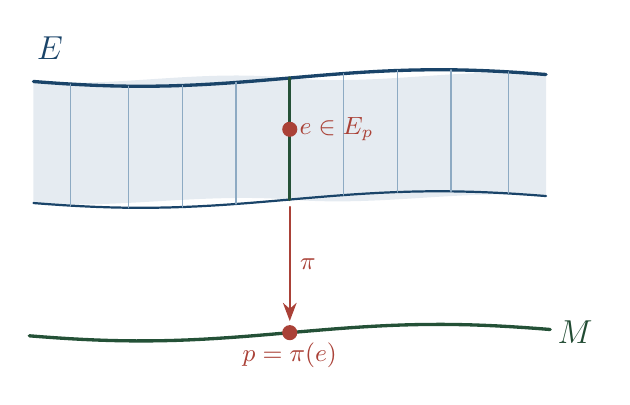
\begin{tikzpicture}[>=Stealth,scale=1.05,line cap=round]
\fill[manifoldblue!12] (-3.1,1.0)
 .. controls (-2.1,.92) and (-1.1,1.15) .. (0,1.04)
 .. controls (1.1,.94) and (2.1,1.18) .. (3.1,1.08)
 --(3.1,-.39)
 .. controls (2.1,-.30) and (1.1,-.52) .. (0,-.43)
 .. controls (-1.1,-.35) and (-2.1,-.55) .. (-3.1,-.47) --cycle;
\draw[manifoldblue!75!black,very thick]
 plot[domain=-3.1:3.1,samples=35] ({\x},{1.04+.10*sin(50*\x)});
\draw[manifoldblue!75!black,thick]
 plot[domain=-3.1:3.1,samples=35] ({\x},{-.43+.10*sin(50*\x)});
\foreach \xx in {-2.65,-1.95,-1.3,-.65,.65,1.3,1.95,2.65}
 \draw[manifoldblue!52,thin] (\xx,{-.43+.10*sin(50*\xx)})
 --(\xx,{1.04+.10*sin(50*\xx)});
\draw[manifoldgreen!65!black,very thick] (0,-.43)--(0,1.04);
\draw[manifoldgreen!65!black,very thick]
 plot[domain=-3.15:3.15,samples=40] ({\x},{-2.04+.10*sin(50*\x)});
\fill[manifoldred] (0,.42) circle (2.6pt) node[right,font=\small] {$e\in E_p$};
\fill[manifoldred] (0,-2.04) circle (2.6pt) node[below,font=\small] {$p=\pi(e)$};
\draw[->,thick,manifoldred] (0,-.52)--(0,-1.9)
 node[midway,right,font=\small] {$\pi$};
\node[manifoldblue!75!black,font=\large\bfseries] at (-2.9,1.4) {$E$};
\node[manifoldgreen!60!black,font=\large\bfseries] at (3.45,-2.03) {$M$};
\end{tikzpicture}
\caption{Lokalny obraz wiązki $\pi\colon E\to M$. Wyróżniono wektor $e$ i jego rzut $\pi(e)=p$. Włókna narysowano jako fragmenty prostych; ogólnie mają wymiar $k$.}
\label{fig:diagram-wiazki}
\end{figure}







Rysunek~\ref{fig:trywializacja} przedstawia lokalną trywializację
z Definicji~\ref{def:wiazka-wektorowa}: zachowuje ona punkt bazy
i jest liniowa na każdym włóknie.

\begin{figure}[ht]
\centering
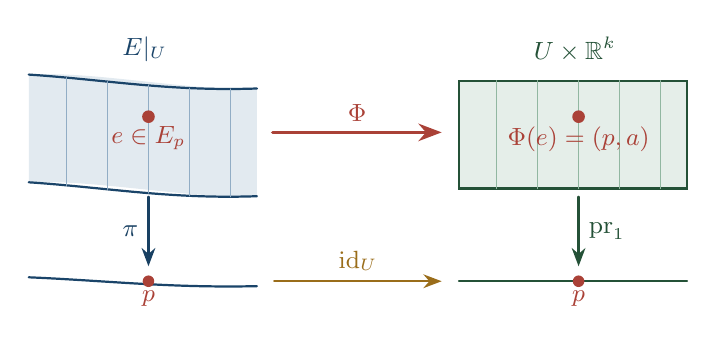
\begin{tikzpicture}[>=Stealth,scale=.95,line cap=round]
\fill[manifoldblue!13] (-4.4,1.16)
 .. controls (-3.55,1.22) and (-2.2,.93) .. (-1.35,.98)
 --(-1.35,-.46)
 .. controls (-2.2,-.51) and (-3.55,-.23) .. (-4.4,-.28) --cycle;
\draw[manifoldblue!75!black,thick]
 plot[domain=-4.4:-1.35,samples=25] ({\x},{1.08+.11*sin(52*\x)});
\draw[manifoldblue!75!black,thick]
 plot[domain=-4.4:-1.35,samples=25] ({\x},{-.36+.11*sin(52*\x)});
\foreach \xx in {-3.9,-3.35,-2.8,-2.25,-1.7}
 \draw[manifoldblue!50,thin] (\xx,{-.36+.11*sin(52*\xx)})
 --(\xx,{1.08+.11*sin(52*\xx)});
\fill[manifoldgreen!13] (1.35,-.36) rectangle (4.4,1.08);
\draw[manifoldgreen!65!black,thick] (1.35,-.36) rectangle (4.4,1.08);
\foreach \xx in {1.85,2.4,2.95,3.5,4.05}
 \draw[manifoldgreen!55,thin] (\xx,-.36)--(\xx,1.08);
\fill[manifoldred] (-2.8,.6) circle (2.4pt)
 node[below,font=\small] {$e\in E_p$};
\fill[manifoldred] (2.95,.6) circle (2.4pt)
 node[below,font=\small] {$\Phi(e)=(p,a)$};
\draw[->,very thick,manifoldred] (-1.14,.39)--(1.12,.39)
 node[midway,above,font=\small] {$\Phi$};
\draw[manifoldblue!75!black,thick]
 plot[domain=-4.4:-1.35,samples=25] ({\x},{-1.6+.07*sin(52*\x)});
\draw[manifoldgreen!65!black,thick] (1.35,-1.6)--(4.4,-1.6);
\fill[manifoldred] (-2.8,-1.6) circle (2.2pt) node[below,font=\small] {$p$};
\fill[manifoldred] (2.95,-1.6) circle (2.2pt) node[below,font=\small] {$p$};
\draw[->,manifoldblue!70!black,thick] (-2.8,-.47)--(-2.8,-1.4)
 node[midway,left,font=\small] {$\pi$};
\draw[->,manifoldgreen!65!black,thick] (2.95,-.47)--(2.95,-1.4)
 node[midway,right,font=\small] {$\operatorname{pr}_1$};
\draw[->,manifoldgold!75!black,thick] (-1.12,-1.6)--(1.12,-1.6)
 node[midway,above,font=\small] {$\mathrm{id}_U$};
\node[manifoldblue!75!black,font=\small\bfseries] at (-2.85,1.5) {$E|_U$};
\node[manifoldgreen!65!black,font=\small\bfseries] at (2.9,1.5) {$U\times\R^k$};
\end{tikzpicture}
\caption{Trywializacja $\Phi\colon E|_U\to U\times\R^k$ jest liniowa na włóknach i zachowuje punkt bazy: $\operatorname{pr}_1\circ\Phi=\pi$. Linie przedstawiają włókna schematycznie.}
\label{fig:trywializacja}
\end{figure}

\begin{definicja}[Sekcja wiązki wektorowej]
\index{sekcja wiazki wektorowej@Sekcja wiązki wektorowej}
Niech $\pi\colon E\to M$ będzie wiązką wektorową. \emph{Sekcją}
(inaczej: \emph{przekrojem}) wiązki $E$ nazywamy
gładkie odwzorowanie $s\colon M\to E$ spełniające $\pi\circ s=\id_M$.
Zatem dla każdego $p\in M$ mamy $s(p)\in E_p$. Sekcja wybiera dokładnie jeden wektor
z każdego włókna i robi to w sposób gładki.
\end{definicja}

\begin{figure}[ht]
\centering
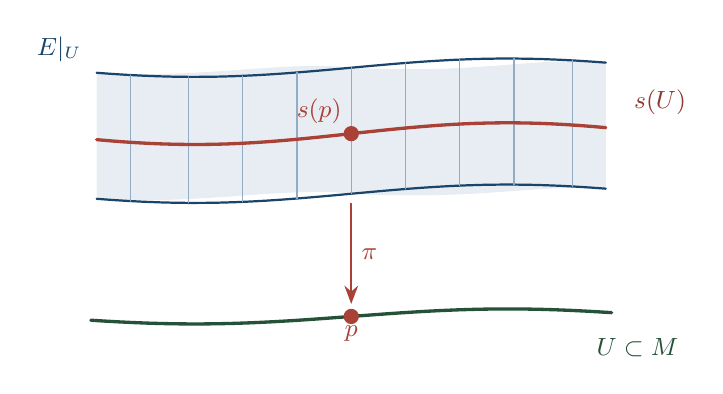
\begin{tikzpicture}[>=Stealth,scale=1.06,line cap=round]
\fill[manifoldblue!11] (-3.05,1.07)
 .. controls (-1.8,.99) and (-.8,1.22) .. (0,1.13)
 .. controls (1.6,1.05) and (2.2,1.27) .. (3.05,1.19)
 --(3.05,-.32)
 .. controls (2.2,-.26) and (1.6,-.46) .. (0,-.38)
 .. controls (-.8,-.29) and (-1.8,-.52) .. (-3.05,-.44) --cycle;
\draw[manifoldblue!75!black,thick]
 plot[domain=-3.05:3.05,samples=34] ({\x},{1.13+.11*sin(48*\x)});
\draw[manifoldblue!75!black,thick]
 plot[domain=-3.05:3.05,samples=34] ({\x},{-.38+.11*sin(48*\x)});
\foreach \xx in {-2.65,-1.95,-1.3,-.65,0,.65,1.3,1.95,2.65}
 \draw[manifoldblue!50,thin] (\xx,{-.38+.11*sin(48*\xx)})
 --(\xx,{1.13+.11*sin(48*\xx)});
\draw[manifoldgreen!65!black,very thick]
 plot[domain=-3.12:3.12,samples=38] ({\x},{-1.85+.09*sin(48*\x)});
\draw[manifoldred,very thick]
 plot[domain=-3.05:3.05,samples=40] ({\x},{.34+.13*sin(48*\x)});
\fill[manifoldred] (0,.34) circle (2.6pt) node[above left,font=\small] {$s(p)$};
\fill[manifoldred] (0,-1.85) circle (2.6pt) node[below,font=\small] {$p$};
\draw[->,manifoldred,thick] (0,-.5)--(0,-1.7)
 node[midway,right,font=\small] {$\pi$};
\node[font=\small\bfseries,manifoldred!85!black] at (3.7,.72) {$s(U)$};
\node[font=\small\bfseries,manifoldgreen!65!black] at (3.43,-2.22) {$U\subset M$};
\node[font=\small,manifoldblue!75!black] at (-3.5,1.35) {$E|_U$};
\end{tikzpicture}
\caption{Sekcja $s$ wybiera dokładnie jeden wektor $s(p)$ w każdym włóknie nad $p$. Czerwona krzywa przedstawia jej obraz nad pokazanym fragmentem $U$.}
\label{fig:sekcja}
\end{figure}

\begin{przyklad}[Sekcja zerowa]
Każda wiązka wektorowa posiada naturalną \emph{sekcję zerową} $s_0\colon M\to E,\ s_0(p)=0_p$,
gdzie $0_p$ jest wektorem zerowym we włóknie $E_p$.
Gładkość wynika z lokalnego zapisu $p\mapsto(p,0)$.
\end{przyklad}


\begin{przyklad}[Wiązka trywialna]
Najprostszym przykładem jest $E=M\times\R^k$ z $\pi=\mathrm{pr}_1$ i $\Psi=\id$ — wiązka ta
nosi nazwę \emph{trywialnej}.
\end{przyklad}

\begin{definicja}[Izomorfizm wiązek wektorowych]
\index{izomorfizm wiazek wektorowych@Izomorfizm wiązek wektorowych}
\label{def:izomorfizm-wiazek}
Niech
$
\pi_E\colon E\to M,
\
\pi_F\colon F\to M
$
będą wiązkami wektorowymi tego samego rzędu nad $M$.
\emph{Izomorfizmem wiązek wektorowych nad $M$} nazywamy
dyfeomorfizm
$
\Phi\colon E\to F
$
taki, że
$
\pi_F\circ\Phi=\pi_E,
$
oraz dla każdego $p\in M$ ograniczenie
$
\Phi_p:=\Phi|_{E_p}\colon E_p\to F_p
$
jest izomorfizmem liniowym.


Warunek
$
\pi_F\circ\Phi=\pi_E
$
oznacza, że $\Phi$ zachowuje punkt bazy: dla każdego $v\in E_p$
mamy
$
\Phi(v)\in F_p.
$
\end{definicja}


\begin{uwaga}
\index{wiazka wektorowa@Wiązka wektorowa!trywialnosc lokalna@trywialność lokalna}
\index{wiazka wektorowa@Wiązka wektorowa!trywialnosc globalna@trywialność globalna}
Każda wiązka wektorowa jest z definicji \emph{lokalnie trywialna}:
dla każdego $p\in M$ istnieje otwarte otoczenie $U\ni p$ takie, że
$
\pi^{-1}(U)\cong U\times\R^k
$
jako wiązki wektorowe nad $U$.

Nie każda wiązka lokalnie trywialna jest jednak globalnie trywialna.
Innymi słowy, z istnienia lokalnych izomorfizmów
$
\pi^{-1}(U)\cong U\times\R^k
$
nie wynika istnienie jednego globalnego izomorfizmu
$
E\cong M\times\R^k.
$
\end{uwaga}
\begin{przyklad}[Wstęga Möbiusa jako nietrywialna wiązka rzędu $1$]
\label{prz:mobius}
\index{wstega Mobiusa\@Wstęga Möbiusa}
\index{wiazka wektorowa\@Wiązka wektorowa!wstega Mobiusa\@wstęga Möbiusa}

Niech
$
M=S^1=\R/2\pi\Z.
$
Na przestrzeni $\R^2=\R\times\R$ definiujemy relację
\[
(x,t)\sim(y,s)
\quad\Longleftrightarrow\quad
\exists k\in\Z
\quad\text{takie, że}\quad
y=x+2\pi k,\qquad s=(-1)^k t.
\]
Definiujemy przestrzeń ilorazową
$
E:=\R^2/\sim.
$
Klasę równoważności punktu $(x,t)\in\R^2$ oznaczamy przez
$
[x,t].
$

Interpretacja tej definicji jest następująca:
przesunięcie pierwszej współrzędnej o jeden pełny obrót, czyli o $2\pi$,
powoduje zmianę znaku drugiej współrzędnej:
$
[x,t]=[x+2\pi,-t].
$
Po dwóch pełnych obrotach znak wraca do pierwotnego:
$
[x,t]=[x+4\pi,t].
$
Właśnie to odwrócenie znaku po jednym obejściu okręgu odpowiada
skręceniu charakterystycznemu dla wstęgi Möbiusa.

Definiujemy rzutowanie $\pi\colon E\longrightarrow S^1, \ \pi([x,t])=[x]$.
Jest ono dobrze określone, ponieważ jeśli
$
(x,t)\sim(y,s),
$
to
$
y=x+2\pi k
$
dla pewnego $k\in\Z$, a więc
$
[y]=[x]
\quad\text{w}\quad
\R/2\pi\Z=S^1.
$

\medskip
\emph{Lokalna trywialność poza punktem sklejenia.}

Niech $I\subset S^1$ będzie otwartym łukiem, który nie zawiera punktu $[0]$.
Możemy wtedy wybrać przedział $(a,b)\subset\R, \ b-a\leq2\pi$,
taki, że każdy punkt $p\in I$ ma dokładnie jednego reprezentanta
$x\in(a,b)$.

Definiujemy
\[
\Psi_I\colon \pi^{-1}(I)\longrightarrow I\times\R,
\qquad
\Psi_I([x,t])=([x],t),
\qquad x\in(a,b).
\]
Odwrotność ma postać $\Psi_I^{-1}([x],t)=[x,t], \ x\in(a,b)$.
Ponieważ na otwartym przedziale długości co najwyżej $2\pi$
nie trzeba przechodzić
przez punkt sklejenia, współrzędna włókna nie zmienia znaku i otrzymujemy
zwykłą lokalną trywializację.

\medskip
\emph{Lokalna trywialność w otoczeniu punktu $[0]$.}

Wybierzmy
$
0<\varepsilon<\pi
$
i rozważmy otwarty łuk
$
I_0:=\{[a]\in S^1:\,-\varepsilon<a<\varepsilon\}.
$
Każdy punkt tego łuku ma dokładnie jednego reprezentanta
$
a\in(-\varepsilon,\varepsilon).
$
Definiujemy odwrotność lokalnej trywializacji przez $\Psi_0^{-1}\colon I_0\times\R\longrightarrow \pi^{-1}(I_0)$,
\[
\Psi_0^{-1}([a],v)=
\begin{cases}
[a,v],& a\ge 0,\\[1mm]
[a+2\pi,-v],& a<0.
\end{cases}
\]

To jest właśnie miejsce, w którym pojawia się zmiana znaku.
Jeżeli $a\ge 0$, to wybieramy reprezentanta $a$ leżącego blisko $0$
z prawej strony i nic nie zmieniamy.
Jeżeli natomiast $a<0$, to aby opisać ten sam punkt okręgu za pomocą
reprezentanta z przedziału bliskiego $2\pi$, musimy zastąpić $a$
przez $a+2\pi$. Z definicji relacji równoważności mamy wtedy
$
[a,v]=[a+2\pi,-v].
$
A zatem przejście od reprezentanta $a$ do reprezentanta $a+2\pi$
wymusza zmianę współrzędnej włókna z $v$ na $-v$.
To nie jest dodatkowa konwencja, lecz bezpośrednia konsekwencja definicji
relacji
$
(x,t)\sim(x+2\pi,-t).
$

Odpowiadająca trywializacja ma postać
\[
\Psi_0([x,t])=
\begin{cases}
([x],t),& -\varepsilon<x<\varepsilon,\\[1mm]
([x-2\pi],-t),& 2\pi-\varepsilon<x<2\pi+\varepsilon.
\end{cases}
\]
W drugim przypadku odejmujemy $2\pi$, aby wrócić do reprezentanta
z przedziału $(-\varepsilon,\varepsilon)$, a współrzędna włókna
musi zmienić znak dokładnie z tego samego powodu co wyżej.

\medskip
\emph{Funkcje przejścia.}

Wybierzmy dwa otwarte łuki $U_0,U_1\subset S^1$, które pokrywają okrąg,
przy czym $U_0$ jest małym łukiem wokół punktu $[0]$, a $U_1=S^1\setminus\{[0]\}$.
Na $U_1$ używamy trywializacji
$
\Psi_1([x,t])=([x],t),
\ x\in(0,2\pi),
$
natomiast na $U_0$ trywializacji $\Psi_0$ zdefiniowanej wyżej.

Przecięcie $U_0\cap U_1$ ma dwie składowe spójne:
jedną w pobliżu punktu $[0]$ od strony dodatniej,
oraz drugą w pobliżu tego samego punktu od strony ujemnej
(czyli po identyfikacji: w pobliżu $2\pi$).

Na składowej dodatniej oba opisy używają tego samego reprezentanta $x$,
więc współrzędna włókna się nie zmienia:
$
v\longmapsto v.
$
Funkcja przejścia jest tam więc równa
$
g=+1.
$

Na składowej ujemnej jedna trywializacja używa reprezentanta bliskiego $0$,
a druga reprezentanta bliskiego $2\pi$.
Przejście między tymi reprezentantami odbywa się przez dodanie lub odjęcie
$2\pi$, a więc z definicji relacji
$
[x,t]=[x+2\pi,-t]
$
współrzędna włókna musi zmienić znak:
$
v\longmapsto -v.
$
Funkcja przejścia jest tam zatem równa
$
g=-1.
$

To dokładnie pokazuje, gdzie geometrycznie pojawia się skręt:
lokalnie mamy produkt $I\times\R$, lecz przy obejściu bazy dookoła
współrzędna włókna wraca z przeciwnym znakiem.

\medskip
Sprawdźmy jeszcze, że otrzymane opisy zgadzają się z topologią
ilorazową $E$. Niech $q:\R^2\to E$ będzie odwzorowaniem ilorazowym.
Jest ono otwarte: dla otwartego $A\subset\R^2$ przeciwobraz
$q^{-1}(q(A))$ jest sumą obrazów $A$ przez homeomorfizmy
$(x,t)\mapsto(x+2\pi k,(-1)^k t)$, $k\in\Z$.
Jeżeli otwarty łuk $I\subset S^1$ jest obrazem przedziału
$J\subset\R$ długości mniejszej niż $2\pi$, to
$q|_{J\times\R}:J\times\R\to\pi^{-1}(I)$ jest bijekcją:
każda klasa ma reprezentanta o pierwszej współrzędnej w $J$,
a dwóch takich reprezentantów nie może różnić przesunięcie
o niezerową wielokrotność $2\pi$. Jest to homeomorfizm,
bo jest ciągły i otwarty. Przejścia między tymi współrzędnymi
mają lokalnie postać
$(x,t)\mapsto(x+2\pi k,(-1)^k t)$ ze stałym $k$,
więc są gładkie.

Punkty nad różnymi punktami bazy rozdzielają przeciwobrazy
rozłącznych łuków w $S^1$. Dwa różne punkty tego samego
włókna rozdzielają otoczenia w jednym z powyższych
otwartych iloczynów. Zatem $E$ jest Hausdorffa.
Przeliczalne pokrycie okręgu takimi łukami i przeliczalne
bazy iloczynów $J\times\R$ dają drugi aksjomat
przeliczalności. W konsekwencji $E$ jest gładką
dwuwymiarową rozmaitością, a odwzorowanie
$
\pi\colon E\to S^1
$
jest gładką rzeczywistą wiązką liniową rzędu $1$.

\end{przyklad}

\begin{figure}[h]
\centering
\begin{minipage}{0.43\textwidth}
\centering
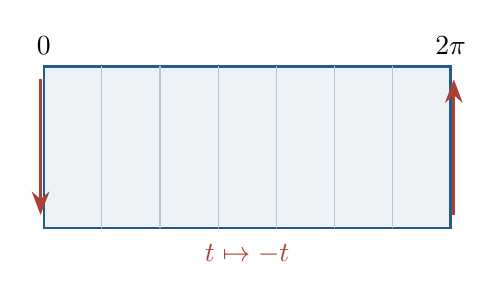
\begin{tikzpicture}[>=Stealth,scale=0.82]
  \fill[manifoldblue!8] (0,-1.25) rectangle (6.3,1.25);
  \draw[thick,manifoldblue] (0,-1.25) rectangle (6.3,1.25);
  \foreach \x in {0.9,1.8,2.7,3.6,4.5,5.4}
    \draw[manifoldblue!35] (\x,-1.25)--(\x,1.25);
  \draw[very thick,->,manifoldred] (-0.05,1.05) -- (-0.05,-1.05);
  \draw[very thick,->,manifoldred] (6.35,-1.05) -- (6.35,1.05);
  \node[above] at (0,1.28) {$0$};
  \node[above] at (6.3,1.28) {$2\pi$};
  \node[manifoldred] at (3.15,-1.65) {$t\mapsto-t$};
\end{tikzpicture}

\smallskip
\small (a) Prostokąt przed sklejeniem
\end{minipage}
\hfill
\begin{minipage}{0.53\textwidth}
\centering
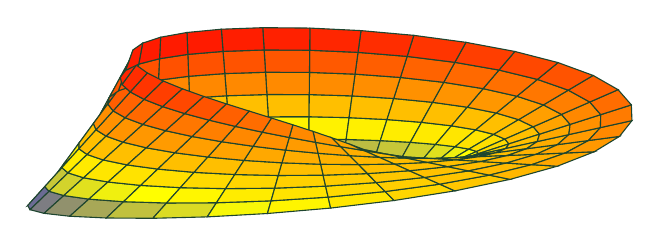
\begin{tikzpicture}
\begin{axis}[
  width=\linewidth,
  height=5.4cm,
  view={55}{25},
  axis lines=none,
  ticks=none,
  z buffer=sort,
  clip=false
]
\addplot3[
  surf,
  shader=faceted,
  faceted color=manifoldgreen!55!black,
  draw=manifoldgreen!70!black,
  domain=0:360,
  y domain=-0.55:0.55,
  samples=34,
  samples y=8
]
({(1+y*cos(x/2))*cos(x)},
 {(1+y*cos(x/2))*sin(x)},
 {y*sin(x/2)});
\end{axis}
\end{tikzpicture}

\smallskip
\small (b) Model geometryczny w $\R^3$
\end{minipage}
\caption{Wstęga Möbiusa: (a) konstrukcja przez sklejenie boków prostokąta z
odwróceniem współrzędnej włókna, (b) odpowiadająca jej klasyczna powierzchnia
zanurzona w $\R^3$. Parametryzacja w części (b) ma postać
$x=(1+t\cos(\theta/2))\cos\theta$,
$y=(1+t\cos(\theta/2))\sin\theta$,
$z=t\sin(\theta/2)$. Rysunek pokazuje tylko pas $|t|\leq0.55$;
w całej wiązce wektorowej $t$ przebiega $\R$.}
\label{fig:mobius}
\end{figure}

\begin{stwierdzenie}[Brak globalnej trywializacji]
\label{prop:mobius-nietrywialna}
\index{wstega Mobiusa\@Wstęga Möbiusa!nietrywialnosc\@nietrywialność}

Wiązka
$
\pi\colon E\to S^1
$
z Przykładu~\ref{prz:mobius} nie jest izomorficzna
z wiązką trywialną
$
S^1\times\R\to S^1.
$
Inaczej mówiąc, nie istnieje globalna trywializacja
$
E\cong S^1\times\R
$
jako wiązek nad $S^1$.
\end{stwierdzenie}

\begin{proof}
Pokażemy najpierw, że każda ciągła sekcja wiązki $E$
musi gdzieś znikać.

Niech
$
s\colon S^1\to E
$
będzie ciągłą sekcją, czyli
$
\pi\circ s=\operatorname{id}_{S^1}.
$
Podnosząc ją do funkcji na $\R$, możemy zapisać
$
s([x])=[x,f(x)]
$
dla pewnej ciągłej funkcji
$
f\colon\R\to\R.
$
Ponieważ
$
[x]=[x+2\pi]
\quad\text{w }S^1,
$
musimy mieć
$
s([x])=s([x+2\pi]).
$
To znaczy
$
[x,f(x)]=[x+2\pi,f(x+2\pi)].
$
Z definicji relacji równoważności wynika stąd
$
f(x+2\pi)=-f(x)
\ \text{dla każdego }x\in\R.
$

Załóżmy teraz, że sekcja $s$ jest nigdzie niezerowa.
Wtedy
$
f(x)\neq 0
\ \text{dla każdego }x\in\R.
$
Jako funkcja ciągła na spójnym zbiorze $\R$,
funkcja $f$ musi mieć stały znak.
W szczególności liczby $f(0)$ i $f(2\pi)$
muszą mieć ten sam znak.

Z drugiej strony z warunku
$
f(2\pi)=-f(0)
$
wynika, że mają znaki przeciwne, o ile tylko $f(0)\neq 0$.
To sprzeczność. Zatem każda ciągła sekcja wiązki $E$
musi mieć co najmniej jedno zero.

Tymczasem wiązka trywialna
$
S^1\times\R\to S^1
$
ma globalną nigdzie niezerową sekcję, na przykład
$
s_1(p)=(p,1).
$

Gdyby istniał izomorfizm wiązek
$
\Phi\colon S^1\times\R\longrightarrow E,
$
to sekcja
$
\Phi\circ s_1
$
byłaby globalną nigdzie niezerową sekcją wiązki $E$.
Jest to niemożliwe na mocy poprzedniego argumentu.

Otrzymujemy sprzeczność. Zatem globalna trywializacja nie istnieje.
\end{proof}

\begin{uwaga}[Znaczenie topologiczne]
Wstęga Möbiusa jest podstawowym przykładem sytuacji, w której
lokalna trywialność nie pociąga za sobą globalnej trywialności.
Na każdym dostatecznie małym łuku
$
I\subset S^1
$
mamy izomorfizm
$
\pi^{-1}(I)\cong I\times\R,
$
jednak nie istnieje jeden globalny izomorfizm
$
E\cong S^1\times\R.
$

Źródłem tej przeszkody jest dokładnie zmiana znaku
$
t\longmapsto -t
$
po jednym pełnym obejściu bazy.
To ona powoduje, że lokalne układy współrzędnych na włóknach
nie mogą zostać sklejone w jeden globalny wybór współrzędnej.
\end{uwaga}

\begin{przyklad}[Wiązka tautologiczna nad $\mathbb{RP}^1$]
\label{prz:tautologiczna-rp1}
\index{wiazka tautologiczna\@Wiązka tautologiczna}
\index{przestrzen rzutowa\@Przestrzeń rzutowa!wiazka tautologiczna\@wiązka tautologiczna}

Przykład wstęgi Möbiusa ma naturalny związek z rzeczywistą
przestrzenią rzutową $\mathbb{RP}^1$.

Przypomnijmy, że $\mathbb{RP}^1$ jest przestrzenią
jednowymiarowych podprzestrzeni liniowych $\R^2$.
Jej punkty zapisujemy w postaci
$
[x_1:x_2],
\ (x_1,x_2)\in\R^2\setminus\{0\},
$
przy czym
$
[x_1:x_2]=[\lambda x_1:\lambda x_2]
\ \text{dla każdego }\lambda\in\R\setminus\{0\}.
$


Każdemu punktowi $[x]\in\mathbb{RP}^1$,
gdzie $x=(x_1,x_2)\neq0$, odpowiada prosta $L_{[x]}:=\operatorname{span}(x) =\{tx:t\in\R\}\subset\R^2$.
Definicja ta nie zależy od wyboru reprezentanta,
ponieważ
$
\operatorname{span}(\lambda x)
=\operatorname{span}(x)
\ (\lambda\neq0).
$

Definiujemy przestrzeń całkowitą
\[
\boxed{
\gamma^1
:=
\bigl\{
([x],v)\in\mathbb{RP}^1\times\R^2:
v\in\operatorname{span}(x)
\bigr\}
}
\]
oraz rzutowanie
\[
\pi_\gamma\colon\gamma^1\longrightarrow\mathbb{RP}^1,
\qquad
\pi_\gamma([x],v)=[x].
\]

Włókno nad punktem $[x]$ ma zatem postać
$
\gamma^1_{[x]}
=
\bigl\{
([x],v):v\in\operatorname{span}(x)
\bigr\}.
$
Po utożsamieniu włókna z jego drugą współrzędną
otrzymujemy
$
\gamma^1_{[x]}\cong\operatorname{span}(x)\cong\R.
$
Poniższe trywializacje pokażą, że otrzymujemy
rzeczywistą wiązkę liniową rzędu $1$,
nazywaną \emph{wiązką tautologiczną}
lub \emph{kanoniczną wiązką liniową} nad $\mathbb{RP}^1$.

Geometrycznie konstrukcja polega na tym, że nad
każdym punktem przestrzeni rzutowej umieszczamy
dokładnie tę prostą w $\R^2$, którą dany punkt
reprezentuje.

\medskip
\emph{Lokalne trywializacje.}

Rozważmy standardowe otwarte podzbiory
$
U_i:=\{[x_1:x_2]\in\mathbb{RP}^1:x_i\neq0\},\ i=1,2.
$


Na $U_1$ używamy współrzędnej $z=\frac{x_2}{x_1}, \ [x_1:x_2]=[1:z]$.
Prosta odpowiadająca punktowi $[1:z]$
jest rozpięta przez wektor $(1,z)$.
Wybierzmy na niej wektor jednostkowy $u_1(z):=\frac{(1,z)}{\sqrt{1+z^2}}$.

Każdy wektor należący do tej prostej
można jednoznacznie zapisać jako
$
v=t\,u_1(z),
\ t\in\R.
$
Ponieważ $u_1(z)$ jest jednostkowy,
współczynnik ten wynosi
$s
t=\langle v,u_1(z)\rangle,
$
gdzie $\langle\cdot,\cdot\rangle$
oznacza standardowy iloczyn skalarny w $\R^2$.

Definiujemy lokalną trywializację
$
\Psi_1\colon
\pi_\gamma^{-1}(U_1)\longrightarrow U_1\times\R
$
wzorem $\Psi_1([1:z],v) = \bigl([1:z],\langle v,u_1(z)\rangle\bigr)$.
Jej odwrotność ma postać $\Psi_1^{-1}([1:z],t) = \bigl([1:z],t\,u_1(z)\bigr)$.

Analogicznie na $U_2$ używamy współrzędnej $w=\frac{x_1}{x_2}, \ [x_1:x_2]=[w:1]$,
i wybieramy wektor jednostkowy $u_2(w):=\frac{(w,1)}{\sqrt{1+w^2}}$.
Otrzymujemy drugą lokalną trywializację $\Psi_2([w:1],v) = \bigl([w:1],\langle v,u_2(w)\rangle\bigr)$,
której odwrotność jest dana przez $\Psi_2^{-1}([w:1],t) = \bigl([w:1],t\,u_2(w)\bigr)$.

Sprawdźmy strukturę gładką przestrzeni całkowitej,
którą na razie traktujemy jako podzbiór
$\mathbb{RP}^1\times\R^2$ z topologią podprzestrzeni.
Nad $U_1$ współrzędne $(z,v_1,v_2)$ spełniają
$v_2=zv_1$. Jest to wykres gładkiej funkcji
$(z,v_1)\mapsto zv_1$, a zatem gładka powierzchnia
w $U_1\times\R^2$. W tych współrzędnych
$t=\langle v,u_1(z)\rangle=v_1\sqrt{1+z^2}$,
więc $\Psi_1$ i jej odwrotność są gładkie.
Analogicznie nad $U_2$ mamy wykres $v_1=wv_2$
oraz $t=v_2\sqrt{1+w^2}$. Obszary $U_1,U_2$
pokrywają $\mathbb{RP}^1$, toteż $\gamma^1$
jest gładką dwuwymiarową podrozmaitością produktu,
a $\Psi_1,\Psi_2$ są lokalnymi trywializacjami
liniowymi na każdym włóknie.

\medskip
\emph{Funkcje przejścia i zmiana znaku.}

Obliczmy funkcję przejścia między
trywializacjami $\Psi_1$ i $\Psi_2$.

Na przecięciu $U_1\cap U_2$ mamy $z\neq0, \ w=\frac1z$.
Zatem
$
u_2(w)=\operatorname{sgn}(z)\,u_1(z)
$
oraz
$
u_2(1/z)=\operatorname{sgn}(z)\,u_1(z).
$

Wyjaśnijmy jej znaczenie.

Jeżeli $z>0$, to
$
u_2(1/z)=u_1(z),
$
a więc oba lokalnie wybrane wektory jednostkowe
mają ten sam zwrot.

Jeżeli natomiast $z<0$, to
$
u_2(1/z)=-u_1(z).
$
Oba wektory rozpinają tę samą prostą,
ale mają przeciwne zwroty.

Niech teraz
$
v=t_1u_1(z)=t_2u_2(1/z).
$
Z poprzedniej równości dostajemy
$
t_1u_1(z)
=
t_2\operatorname{sgn}(z)u_1(z),
$
a zatem
$
t_2=\operatorname{sgn}(z)t_1.
$

Funkcja przejścia ma więc postać
\[
\boxed{
g_{21}([1:z])
=
\begin{cases}
+1,&z>0,\\
-1,&z<0.
\end{cases}
}
\]

Przecięcie $U_1\cap U_2$ ma dwie składowe
spójności, odpowiadające $z>0$ oraz $z<0$.
Na jednej z nich współrzędna włókna
pozostaje niezmieniona, a na drugiej
zmienia znak.

Zmiana znaku nie oznacza zmiany samego
wektora $v\in\R^2$.
Wektor ten pozostaje ten sam.
Zmienia się jedynie jego współrzędna
względem innego wyboru wektora jednostkowego
rozpinającego tę samą prostą.

W szczególności
$
v=t\,u=(-t)(-u).
$
Ta prosta równość algebraiczna wyjaśnia
geometrycznie występowanie funkcji przejścia
równej $-1$.

\medskip
\emph{Identyfikacja $\mathbb{RP}^1$ z okręgiem.}

Pokażemy teraz, że wiązka $\gamma^1$
jest izomorficzna z wstęgą Möbiusa
skonstruowaną w Przykładzie~\ref{prz:mobius}.


Zdefiniujmy odwzorowanie
$
F\colon S^1\longrightarrow\mathbb{RP}^1
$
wzorem $F([\theta]) = [\cos(\theta/2):\sin(\theta/2)]$.

Najpierw sprawdźmy, że jest ono dobrze określone.
Jeżeli
$
[\theta]=[\varphi]\in S^1,
$
to
$
\varphi=\theta+2\pi k
$
dla pewnego $k\in\Z$.
Wówczas
\[
\begin{aligned}
\cos(\varphi/2)
&=\cos(\theta/2+\pi k)
=(-1)^k\cos(\theta/2),\\
\sin(\varphi/2)
&=\sin(\theta/2+\pi k)
=(-1)^k\sin(\theta/2).
\end{aligned}
\]
Ponieważ w przestrzeni rzutowej
utożsamiamy niezerowe wielokrotności
tego samego wektora, otrzymujemy
$
[\cos(\varphi/2):\sin(\varphi/2)]
=
[\cos(\theta/2):\sin(\theta/2)].
$

Pokażemy, że $F$ jest dyfeomorfizmem.

Różnowartościowość wynika z faktu, że
jeśli
$
[\cos(\theta/2):\sin(\theta/2)]
=
[\cos(\varphi/2):\sin(\varphi/2)],
$
to odpowiadające im wektory jednostkowe
różnią się co najwyżej znakiem:
\[
\begin{pmatrix}
\cos(\varphi/2)\\
\sin(\varphi/2)
\end{pmatrix}
=
\pm
\begin{pmatrix}
\cos(\theta/2)\\
\sin(\theta/2)
\end{pmatrix}.
\]
Stąd
$
\frac{\varphi}{2}
=
\frac{\theta}{2}+\pi k
$
dla pewnego $k\in\Z$, czyli
$
\varphi=\theta+2\pi k.
$
A zatem $[\varphi]=[\theta]$.

Aby wykazać surjektywność, weźmy dowolny
punkt $[x_1:x_2]\in\mathbb{RP}^1$.
Normalizując jego reprezentanta, możemy zapisać $\frac{(x_1,x_2)}{\sqrt{x_1^2+x_2^2}} = (\cos\alpha,\sin\alpha)$
dla pewnego $\alpha\in\R$.
Wtedy
$
F([2\alpha])
=
[\cos\alpha:\sin\alpha]
=
[x_1:x_2].
$

Dla pełności wskażmy również gładką
odwrotność. Utożsamiając $S^1$
z okręgiem jednostkowym w $\mathbb C$,
otrzymujemy wzór
\[
\boxed{
F^{-1}([x_1:x_2])
=
\frac{(x_1+ix_2)^2}{x_1^2+x_2^2}.
}
\]
Wyrażenie po prawej stronie należy do $S^1$,
ponieważ jego moduł wynosi $1$.
Nie zależy ono od reprezentanta:
zastąpienie $(x_1,x_2)$ przez
$(\lambda x_1,\lambda x_2)$ mnoży
licznik i mianownik przez $\lambda^2$.

Jeżeli
$
(x_1,x_2)=(\cos\alpha,\sin\alpha),
$
to
$
F^{-1}([x_1:x_2])
=(\cos\alpha+i\sin\alpha)^2
=e^{2i\alpha}.
$
Widzimy więc, że jest to rzeczywiście
odwrotność $F$.

Zarówno $F$, jak i $F^{-1}$
są gładkie w lokalnych współrzędnych,
a zatem
$
S^1\cong\mathbb{RP}^1
$
jako rozmaitości gładkie.

\medskip
\emph{Jawny izomorfizm wiązek.}

Dla $\theta\in\R$ oznaczmy
\[
u(\theta)
:=
\begin{pmatrix}
\cos(\theta/2)\\
\sin(\theta/2)
\end{pmatrix}.
\]
Jest to wektor jednostkowy rozpinający
prostą odpowiadającą punktowi $F([\theta])$.

Zdefiniujmy odwzorowanie
$
\Phi\colon E\longrightarrow\gamma^1
$
wzorem
\[
\Phi([\theta,t])
=
\bigl(
[\cos(\theta/2):\sin(\theta/2)],
t\,u(\theta)
\bigr).
\]

Wartość $\Phi([\theta,t])$ rzeczywiście
należy do $\gamma^1$, ponieważ
$
t\,u(\theta)
\in\operatorname{span}(u(\theta)).
$

Sprawdźmy dokładnie, że $\Phi$
jest dobrze określone na klasach równoważności.

Jeżeli
$
(\theta,t)\sim(\varphi,s),
$
to dla pewnego $k\in\Z$ mamy
$
\varphi=\theta+2\pi k,
\ 
s=(-1)^k t.
$
Jednocześnie
$
u(\varphi)
=
u(\theta+2\pi k)
=
(-1)^k u(\theta).
$
Stąd
$
s\,u(\varphi)=t\,u(\theta).
$
Ponadto
$
[u(\varphi)]=[u(\theta)]
\ \text{w }\mathbb{RP}^1.
$
W konsekwencji
$
\Phi([\varphi,s])=\Phi([\theta,t]).
$
Odwzorowanie $\Phi$ jest więc
dobrze określone.

W szczególności dla jednego pełnego obrotu
otrzymujemy rachunek
\[
\begin{aligned}
\Phi([\theta+2\pi,-t])
&=
\bigl([u(\theta+2\pi)],-t\,u(\theta+2\pi)\bigr)\\
&=
\bigl([-u(\theta)],(-t)(-u(\theta))\bigr)\\
&=
\bigl([u(\theta)],t\,u(\theta)\bigr)\\
&=\Phi([\theta,t]).
\end{aligned}
\]
Widzimy zatem, że zmiana znaku
współrzędnej włókna w definicji wstęgi Möbiusa
jest dokładnie kompensowana zmianą znaku
wektora jednostkowego reprezentującego
punkt przestrzeni rzutowej.

Odwzorowanie $\Phi$ zachowuje rzutowania,
gdyż
\[
\begin{aligned}
\pi_\gamma(\Phi([\theta,t]))
&=[\cos(\theta/2):\sin(\theta/2)]\\
&=F([\theta])\\
&=F(\pi([\theta,t])).
\end{aligned}
\]

Otrzymujemy więc przemienny diagram
\begin{center}
\begin{tikzcd}
E \arrow[r,"\Phi"] \arrow[d,"\pi"']
&
\gamma^1 \arrow[d,"\pi_\gamma"]
\\
S^1 \arrow[r,"F"']
&
\mathbb{RP}^1
\end{tikzcd}
\end{center}
Pokażemy teraz, że $\Phi$ jest bijekcją.
Niech
$
([x],v)\in\gamma^1.
$
Wybierzmy jednostkowy wektor $u$
rozpinający prostą $[x]$.
Możemy zapisać
$
u=(\cos\alpha,\sin\alpha)
$
dla pewnego $\alpha\in\R$.
Ponieważ $v\in\operatorname{span}(u)$,
istnieje dokładnie jedna liczba $t\in\R$
taka, że
$
v=tu.
$
Jest nią
$
t=\langle v,u\rangle.
$
Wówczas
$
\Phi([2\alpha,t])
=
([u],tu)
=
([x],v),
$
co dowodzi surjektywności.

Sprawdźmy również, że otrzymana klasa
$[2\alpha,t]\in E$ nie zależy od wyboru
wektora jednostkowego $u$.

Na tej samej prostej istnieją dokładnie
dwa wektory jednostkowe: $u$ oraz $-u$.
Jeżeli zastąpimy $u$ przez $-u$, to możemy
zastąpić $\alpha$ przez $\alpha+\pi$,
natomiast współczynnik $t$ przez $-t$:
$
v=tu=(-t)(-u).
$
Otrzymujemy wtedy parę
$
(2\alpha+2\pi,-t),
$
która jest równoważna z $(2\alpha,t)$,
ponieważ
$
(2\alpha,t)\sim(2\alpha+2\pi,-t).
$
Dodanie do $\alpha$ całkowitej wielokrotności
$2\pi$ również nie zmienia klasy w $E$.

Możemy zatem zdefiniować odwrotność $\Phi^{-1}([x],v) = [2\alpha,\langle v,u\rangle]$,
gdzie $u=(\cos\alpha,\sin\alpha)$
jest dowolnym wektorem jednostkowym
rozpinającym $[x]$.

Wykazaliśmy, że wzór ten nie zależy
od dokonanych wyborów.
Bezpośrednio otrzymujemy
\[
\Phi^{-1}\circ\Phi=\operatorname{id}_E,
\qquad
\Phi\circ\Phi^{-1}=\operatorname{id}_{\gamma^1}.
\]

Pozostaje uzasadnić gładkość.

Wybierzmy dostatecznie mały otwarty łuk
$I\subset S^1$, na którym można gładko
wybrać reprezentanta kąta $\theta$.
Na $\pi^{-1}(I)$ używamy trywializacji
wstęgi Möbiusa zapisującej każdy punkt
jednoznacznie jako $[\theta,t]$.

Na odpowiadającym mu obszarze $F(I)\subset\mathbb{RP}^1$
wybieramy gładki wektor jednostkowy
$
u(F([\theta]))=u(\theta).
$
Otrzymujemy wówczas trywializację
wiązki tautologicznej $([x],v)\longmapsto ([x],\langle v,u([x])\rangle)$.

W tych lokalnych trywializacjach
odwzorowanie $\Phi$ ma szczególnie prostą postać:
$
([\theta],t)\longmapsto(F([\theta]),t).
$
Jest więc gładkie, ponieważ $F$
jest dyfeomorfizmem.
Jego lokalna odwrotność ma postać
$
([x],t)\longmapsto(F^{-1}([x]),t)
$
i również jest gładka.

Ponadto na każdym włóknie $\Phi$
jest izomorfizmem liniowym:
$
t\longmapsto t\,u(\theta).
$

Ostatecznie $\Phi$ jest izomorfizmem
gładkich wiązek wektorowych nad
dyfeomorfizmem baz $F$:
\[
(E\xrightarrow{\pi}S^1)
\cong
(\gamma^1\xrightarrow{\pi_\gamma}\mathbb{RP}^1).
\]
Definicja~\ref{def:izomorfizm-wiazek} dotyczy wiązek
nad tą samą bazą; tutaj utożsamiamy bazy przez $F$,
a równanie $\pi_\gamma\circ\Phi=F\circ\pi$
zastępuje warunek zachowania punktu bazy.

\medskip
\emph{Geometryczna interpretacja skręcenia.}

Wyjaśnijmy jeszcze, dlaczego w tej konstrukcji
naturalnie pojawia się wstęga Möbiusa,
a nie wiązka trywialna.

Punkt $F([\theta]) = [\cos(\theta/2):\sin(\theta/2)]$
reprezentuje prostą przechodzącą przez początek
układu współrzędnych, tworzącą z dodatnią
półosią poziomą kąt $\theta/2$.

Kiedy $\theta$ przebiega przedział
$[0,2\pi]$, prosta wykonuje obrót o kąt $\pi$.
Jest to pełne obejście przestrzeni $\mathbb{RP}^1$,
ponieważ proste rozpięte przez $u$ i $-u$
są identyczne.

Jednak wybrany w sposób ciągły
wektor jednostkowy
$
u(\theta)
=
(\cos(\theta/2),\sin(\theta/2))
$
nie wraca do swojej początkowej wartości: $u(0)=(1,0),\ u(2\pi)=(-1,0)=-u(0)$.

Aby ten sam wektor $v$ we włóknie
przedstawić po pełnym obejściu bazy,
jego współczynnik musi więc zmienić znak:
$
v=t\,u(0)=(-t)\,u(2\pi).
$
Otrzymujemy dokładnie identyfikację
$
(0,t)\sim(2\pi,-t)
$
charakterystyczną dla wstęgi Möbiusa.

\medskip
\emph{Nietrywialność wiązki tautologicznej.}

Z wykazanego izomorfizmu i
Stwierdzenia~\ref{prop:mobius-nietrywialna}
wynika już, że $\gamma^1$ nie jest trywialna.
Można to również zobaczyć bezpośrednio
z jej geometrycznej konstrukcji.

Przypuśćmy, że istnieje globalna
nigdzie niezerowa ciągła sekcja
$
s\colon\mathbb{RP}^1\longrightarrow\gamma^1.
$
Dla $\theta\in[0,2\pi]$ możemy zapisać $s(F([\theta])) = \bigl(F([\theta]),a(\theta)u(\theta)\bigr)$,
gdzie $a\colon[0,2\pi]\to\R$
jest funkcją ciągłą.

Ponieważ
$
F([0])=F([2\pi]),
$
wartości przekroju na końcach przedziału
muszą być równe:
$
a(0)u(0)=a(2\pi)u(2\pi).
$
Korzystając z równości
$
u(2\pi)=-u(0),
$
otrzymujemy
$
a(0)u(0)=-a(2\pi)u(0),
$
a więc
$
a(2\pi)=-a(0).
$

Z twierdzenia o wartości pośredniej
wynika, że funkcja $a$ musi mieć zero
w przedziale $[0,2\pi]$.
Istnieje zatem $\theta_0$ takie, że
$
a(\theta_0)=0,
$
czyli
$
s(F([\theta_0]))
=
(F([\theta_0]),0).
$
Jest to sprzeczne z założeniem,
że przekrój jest nigdzie niezerowy.

Tymczasem każda trywialna wiązka
liniowa rzędu $1$ posiada globalny
nigdzie niezerowy przekrój.

W konsekwencji
$
\gamma^1\not\cong\mathbb{RP}^1\times\R
$
jako wiązki wektorowe nad $\mathbb{RP}^1$.

Wiązka tautologiczna nad $\mathbb{RP}^1$
jest więc dokładnie tą samą
nietrywialną wiązką liniową,
którą geometrycznie opisuje wstęga Möbiusa.
\end{przyklad}

\subsection*{Wiązka styczna}

Pokażemy, że zbiór $TM:=\bigsqcup_{p\in M}T_pM$
można w naturalny sposób wyposażyć w strukturę rozmaitości gładkiej
wymiaru $2n$, tak by rzutowanie $\pi\colon TM\to M, \ \pi(v)=p \quad\text{dla }v\in T_pM$,
było wiązką wektorową rzędu $n$.
Punkt $p=\pi(v)$ nazywamy \emph{podstawą}, natomiast
$T_pM=\pi^{-1}(p)$ jest włóknem wiązki stycznej nad $p$.

Niech $\{(U_\alpha,\varphi_\alpha)\}$ będzie atlasem na $M$,
$\varphi_\alpha=(x^1_\alpha,\dots,x^n_\alpha)$.
Definiujemy $\tilde U_\alpha:=\pi^{-1}(U_\alpha)\subseteq TM$
oraz
\[
\tilde\varphi_\alpha\colon
\tilde U_\alpha\to
\varphi_\alpha(U_\alpha)\times\R^n\subseteq\R^{2n},
\]
\[
\tilde\varphi_\alpha\Big(
\sum_{i=1}^n v^i
\left.\frac{\partial}{\partial x^i_\alpha}\right|_p
\Big)
:=
(\varphi_\alpha(p),v^1,\dots,v^n).
\]

Każde $\tilde\varphi_\alpha$ jest bijekcją na $\varphi_\alpha(U_\alpha)\times\R^n$
(dla ustalonego $p$, współrzędne $v^i$ względem bazy $\{\partial/\partial x^i_\alpha|_p\}$
wyznaczają bijekcję liniową $T_pM\to\R^n$).

Z reguły transformacji~\eqref{eq:transformacja-derywacji} wynika,
że dla $x\in\varphi_\alpha(U_\alpha\cap U_\beta)$ i $v\in\R^n$
odwzorowanie przejścia ma postać
\[
\big(\tilde\varphi_\beta\circ\tilde\varphi_\alpha^{-1}\big)(x,v)=\Big(
(\varphi_\beta\circ\varphi_\alpha^{-1})(x),\ D(\varphi_\beta\circ\varphi_\alpha^{-1})(x)
\cdot v\Big).
\]
Najpierw określamy topologię na $TM$: zbiór $A\subset TM$
jest otwarty wtedy i tylko wtedy, gdy każdy
$\tilde\varphi_\alpha(A\cap\tilde U_\alpha)$ jest otwarty.
Zmiany współrzędnych powyżej są homeomorfizmami, a ich dziedziny
$\varphi_\alpha(U_\alpha\cap U_\beta)\times\R^n$ są otwarte.
Wynika stąd, że $\tilde U_\alpha$ są otwarte, a
$\tilde\varphi_\alpha$ są homeomorfizmami: obraz dowolnego otwartego
zbioru z jednej mapy jest otwarty także w każdej nakładającej się mapie.
Rzutowanie $\pi$ jest ciągłe, bo lokalnie ma postać $(x,v)\mapsto x$.
Gładkość zmiany współrzędnych wynika z reguły
\eqref{eq:transformacja-derywacji}. Zatem $\{(\tilde
U_\alpha,\tilde\varphi_\alpha)\}$ jest atlasem na $TM$. Punkty o różnych
podstawach rozdzielają przeciwobrazy rozłącznych otoczeń w $M$;
dwa różne wektory w jednym włóknie rozdzielają kule w jednej mapie
$\tilde\varphi_\alpha$. Stąd $TM$ jest Hausdorffa. Z przeliczalności
bazy $M$ wybieramy przeliczalną rodzinę dziedzin map pokrywającą $M$.
Obrazy tych map w $TM$ mają przeliczalne bazy euklidesowe, których
przeciwobrazy tworzą przeliczalną bazę $TM$.

Tak skonstruowana rozmaitość $TM$, wraz z rzutowaniem $\pi$ i lokalnymi trywializacjami
$\Psi_\alpha=(\varphi_\alpha^{-1}\times\id)\circ\tilde\varphi_\alpha$, jest wiązką
wektorową rzędu $n$ nad $M$ — \emph{wiązką styczną}.

\subsection*{Wiązka kostyczna}

Definiujemy teraz \emph{wiązkę kostyczną}
$T^*M:=\bigsqcup_{p\in M}T_p^*M$ oraz rzutowanie
$\pi^*\colon T^*M\to M$, $\pi^*(\omega)=p$ dla $\omega\in T_p^*M$.
Nad $U_\alpha$ określamy mapę
\[
\tilde\varphi_\alpha^*\Big(\sum_i\xi_i\,dx^i_\alpha|_p\Big)
:=(\varphi_\alpha(p),\xi_1,\ldots,\xi_n).
\]
Jest ona bijekcją na $\varphi_\alpha(U_\alpha)\times\R^n$,
ponieważ $\{dx^i_\alpha|_p\}$ jest bazą każdego włókna.
Dla $x\in\varphi_\alpha(U_\alpha\cap U_\beta)$
reguła~\eqref{eq:transformacja-wspolrzednych-kowektora} daje
\[
\big(\tilde\varphi_\beta^*\circ(\tilde\varphi_\alpha^*)^{-1}\big)(x,\xi)
=\Big(\varphi_\beta\circ\varphi_\alpha^{-1}(x),
D(\varphi_\beta\circ\varphi_\alpha^{-1})(x)^{-\mathsf T}\xi\Big).
\]
Pochodna odwzorowania przejścia jest gładka i odwracalna,
więc również jej odwrotna transpozycja zależy gładko od $x$.
Wzory te pozwalają określić topologię i atlas na $T^*M$
tak samo jak dla $TM$; są też liniowe na każdym włóknie.
Dowód, że $T^*M$ jest wiązką wektorową rzędu $n$ nad $M$,
dopełnia to samo sprawdzenie:
punkty o różnych podstawach rozdzielają przeciwobrazy otoczeń bazy,
punkty jednego włókna rozdzielają kule współrzędnych dualnych; bazy
euklidesowe w przeliczalnym pokryciu map dają drugi aksjomat przeliczalności.

\begin{definicja}
\emph{Polem wektorowym} na $M$ nazywamy gładką sekcję wiązki stycznej, tzn.\ gładkie
odwzorowanie $X\colon M\to TM$ z $\pi\circ X=\id_M$ (a więc $X(p)\in T_pM$ dla każdego
$p$). \emph{Polem kowektorowym} na $M$ nazywamy gładką sekcję wiązki kostycznej $T^*M$.
\end{definicja}

\section{Funkcje przejścia i operacje na wiązkach}

Lokalna trywialność pozwala opisywać wiązkę macierzami. Ta postać jest
szczególnie użyteczna przy konstruowaniu wiązek normalnych podrozmaitości.

Niech $\Psi_i:E|_{U_i}\to U_i\times\R^r$ będą trywializacjami.
Dla każdego $p\in U_i$ mają one postać $\Psi_i(e)=(p,\psi_{i,p}(e)),\ e\in E_p$,
gdzie $\psi_{i,p}:E_p\to\R^r$ jest izomorfizmem liniowym.
Na przecięciu $U_i\cap U_j$ otrzymujemy więc zmianę trywializacji daną wzorem $\Psi_j\circ\Psi_i^{-1}(p,v)=(p,g_{ji}(p)v)$,
gdzie $g_{ji}(p)\in\mathrm{GL}(r,\R)$ jest macierzą izomorfizmu
liniowego $\psi_{j,p}\circ\psi_{i,p}^{-1}$.
W ten sposób otrzymujemy gładkie odwzorowania $g_{ji}:U_i\cap U_j\longrightarrow\mathrm{GL}(r,\R)$,
zwane \emph{funkcjami przejścia}. Na przecięciach spełniają one
\begin{equation}\label{eq:warunek-kocyklu-wiazki}
g_{ii}=I,\qquad g_{ij}=g_{ji}^{-1},\qquad
g_{ki}=g_{kj}g_{ji}\quad\text{na }U_i\cap U_j\cap U_k.
\end{equation}
Ostatnia równość porównuje bezpośrednie przejście z $i$ do $k$
z przejściem przez $j$; nazywamy ją warunkiem kocyklu.


\begin{twierdzenie}[Sklejanie wiązki z funkcji przejścia]
Niech $\{U_i\}$ będzie otwartym pokryciem rozmaitości $M$, a gładkie funkcje
$g_{ji}:U_i\cap U_j\to\mathrm{GL}(r,\R)$ spełniają
warunek~\eqref{eq:warunek-kocyklu-wiazki}. Wtedy istnieje
wiązka wektorowa rzędu $r$ o tych funkcjach przejścia.
\end{twierdzenie}

\begin{proof}
Na sumie rozłącznej $Z:=\bigsqcup_i(U_i\times\R^r)$ wprowadzamy relację
\[
(p,v)_i\sim(p,w)_j
\quad\Longleftrightarrow\quad
p\in U_i\cap U_j,\quad w=g_{ji}(p)v.
\]
Jest to relacja równoważności: pierwsza i druga tożsamość
w~\eqref{eq:warunek-kocyklu-wiazki}
dają zwrotność i symetrię, trzecia zaś przechodniość.

Niech $E:=Z/\sim$ będzie zbiorem klas równoważności i określmy
$\pi:E\to M$ wzorem $\pi([p,v]_i)=p$.
Dla każdego $i$ definiujemy odwzorowanie
\[
\Psi_i:\pi^{-1}(U_i)\longrightarrow U_i\times\R^r,
\qquad
\Psi_i([p,v]_j)=(p,g_{ij}(p)v).
\]
Jest ono dobrze określone: jeżeli $(p,v)_j\sim(p,w)_k$, to
$w=g_{kj}(p)v$, a z warunku kocyklu wynika $g_{ik}(p)w =g_{ik}(p)g_{kj}(p)v =g_{ij}(p)v$.
Ponadto $\Psi_i$ jest bijekcją, której odwrotność ma postać $\Psi_i^{-1}(p,v)=[p,v]_i$.

Nadajemy teraz $E$ topologię, przyjmując, że zbiór $A\subset E$
jest otwarty wtedy i tylko wtedy, gdy dla każdego $i$ zbiór $\Psi_i\bigl(A\cap\pi^{-1}(U_i)\bigr)$
jest otwarty w $U_i\times\R^r$.
Warunki te rzeczywiście określają topologię: zbiór pusty i całe $E$
są otwarte, a ponieważ każde $\Psi_i$ jest bijekcją,
obrazy sum dowolnych rodzin oraz przecięć skończonych
odpowiadają odpowiednio sumom i przecięciom ich obrazów.

Wykażemy, że każda $\Psi_i$ jest homeomorfizmem.

Najpierw zauważmy, że $\pi^{-1}(U_i)$ jest zbiorem otwartym
w $E$. Istotnie, dla każdego $j$ mamy
\[
\Psi_j\bigl(
\pi^{-1}(U_i)\cap\pi^{-1}(U_j)
\bigr)
=(U_i\cap U_j)\times\R^r,
\]
a zbiór po prawej stronie jest otwarty w $U_j\times\R^r$.

Niech następnie $V\subset U_i\times\R^r$ będzie otwarty.
Zbadamy otwartość zbioru $\Psi_i^{-1}(V)$ w $E$.
Dla każdego $j$ zachodzi
\[
\begin{aligned}
&\Psi_j\bigl(
\Psi_i^{-1}(V)\cap\pi^{-1}(U_j)
\bigr)\\
&\qquad =
(\Psi_j\circ\Psi_i^{-1})
\bigl(V\cap((U_i\cap U_j)\times\R^r)\bigr).
\end{aligned}
\]
Odwzorowanie przejścia ma postać $\Psi_j\circ\Psi_i^{-1}(p,v) =(p,g_{ji}(p)v)$.
Jest ono homeomorfizmem zbioru
$(U_i\cap U_j)\times\R^r$ na siebie, gdyż $g_{ji}$
jest gładka, a odwrotność jest dana wzorem $(p,w)\longmapsto(p,g_{ij}(p)w)$.
Wobec tego rozważany obraz jest otwarty w
$(U_i\cap U_j)\times\R^r$, a więc również
w $U_j\times\R^r$. Z definicji topologii na $E$
wynika, że $\Psi_i^{-1}(V)$ jest otwarty.
Dowodzi to ciągłości $\Psi_i$.

Z drugiej strony, jeżeli
$A\subset\pi^{-1}(U_i)$ jest otwarty, to jest również
otwarty w $E$, ponieważ $\pi^{-1}(U_i)$ jest otwarty.
Z definicji topologii otrzymujemy, że $\Psi_i(A) =\Psi_i\bigl(A\cap\pi^{-1}(U_i)\bigr)$
jest otwarty w $U_i\times\R^r$.
Zatem $\Psi_i$ jest odwzorowaniem otwartym.
Ponieważ jest także ciągłą bijekcją, jest homeomorfizmem.

Skonstruujemy teraz na $E$ gładki atlas wymiaru
$\dim M+r$. Niech $(W_\alpha,\varphi_\alpha)$ będzie
mapą rozmaitości $M$ i oznaczmy $n:=\dim M$.
Na zbiorze $\pi^{-1}(U_i\cap W_\alpha)$ definiujemy
\[
\widetilde\varphi_{i\alpha}
:=
(\varphi_\alpha\times\operatorname{id}_{\R^r})
\circ\Psi_i.
\]
Jest to homeomorfizm na otwarty podzbiór $\varphi_\alpha(U_i\cap W_\alpha)\times\R^r \subset\R^{n+r}$.
Otrzymane odwzorowania tworzą atlas topologiczny na $E$.

Na przecięciu dziedzin dwóch takich map
zmiana współrzędnych ma postać
\[
\begin{aligned}
&\widetilde\varphi_{j\beta}
\circ\widetilde\varphi_{i\alpha}^{-1}(x,v)\\
&\qquad =
\Bigl(
\varphi_\beta\circ\varphi_\alpha^{-1}(x),
g_{ji}(\varphi_\alpha^{-1}(x))v
\Bigr).
\end{aligned}
\]
Jest ona gładka, ponieważ zmiany współrzędnych na
$M$ oraz funkcje przejścia $g_{ji}$ są gładkie.
Jej odwrotność otrzymujemy przez zamianę
$(i,\alpha)$ z $(j,\beta)$, zatem także jest gładka.
Otrzymany atlas jest gładki.

Włókna $E_p=\pi^{-1}(\{p\})$ wyposażamy w działania
liniowe przeniesione z $\R^r$ przez dowolną
trywializację $\Psi_i$, dla której $p\in U_i$.
Działania te nie zależą od wyboru trywializacji,
ponieważ wszystkie funkcje przejścia $g_{ji}(p)$
są izomorfizmami liniowymi.
Ponadto w lokalnych współrzędnych rzutowanie
$\pi$ przyjmuje postać $(x,v)\longmapsto x$,
jest więc gładkie.

Pozostaje uzasadnić, że $E$ jest przestrzenią
Hausdorffa i spełnia drugi aksjomat przeliczalności.

Najpierw zauważmy, że $\pi$ jest ciągłe.
Istotnie, dla każdego otwartego $O\subset M$ mamy
\[
\Psi_i\bigl(
\pi^{-1}(O)\cap\pi^{-1}(U_i)
\bigr)
=(O\cap U_i)\times\R^r,
\]
co jest zbiorem otwartym w $U_i\times\R^r$.
Zatem $\pi^{-1}(O)$ jest otwarty w $E$.

Niech $e_1,e_2\in E$ będą różnymi punktami.
Jeżeli $\pi(e_1)\ne\pi(e_2)$, to ponieważ $M$
jest przestrzenią Hausdorffa, istnieją rozłączne
otwarte otoczenia $V_1,V_2\subset M$ punktów
$\pi(e_1)$ i $\pi(e_2)$. Wówczas
$\pi^{-1}(V_1)$ i $\pi^{-1}(V_2)$ są rozłącznymi
otwartymi otoczeniami punktów $e_1$ i $e_2$.

Jeżeli natomiast $\pi(e_1)=\pi(e_2)=p$,
wybieramy $i$ takie, że $p\in U_i$.
Ponieważ $\Psi_i$ jest bijekcją, istnieją różne
$v_1,v_2\in\R^r$ takie, że $\Psi_i(e_1)=(p,v_1), \ \Psi_i(e_2)=(p,v_2)$.
Wybieramy rozłączne otwarte kule
$B_1,B_2\subset\R^r$ wokół $v_1$ i $v_2$.
Wówczas $\Psi_i^{-1}(U_i\times B_1), \ \Psi_i^{-1}(U_i\times B_2)$
są rozłącznymi otwartymi otoczeniami
punktów $e_1$ i $e_2$.
Stąd $E$ jest przestrzenią Hausdorffa.

Na koniec wykażemy drugi aksjomat przeliczalności.
Ponieważ $M$ ma przeliczalną bazę topologii,
pokrycie $\{U_i\}$ ma przeliczalne podpokrycie
$\{U_{i_k}\}_{k\in\N}$.
Każda przestrzeń $U_{i_k}\times\R^r$ ma
przeliczalną bazę $\mathcal B_k$.
Ponieważ $\Psi_{i_k}$ jest homeomorfizmem
i $\pi^{-1}(U_{i_k})$ jest otwarty w $E$,
rodzina
\[
\mathcal B:=
\bigcup_{k\in\N}
\left\{
\Psi_{i_k}^{-1}(B):B\in\mathcal B_k
\right\}
\]
jest przeliczalną rodziną zbiorów otwartych w $E$.

Jest ona bazą topologii na $E$. Istotnie, jeżeli
$A\subset E$ jest otwarty i $e\in A$, to istnieje
$k$ takie, że $\pi(e)\in U_{i_k}$.
Zbiór $\Psi_{i_k}\bigl( A\cap\pi^{-1}(U_{i_k}) \bigr)$
jest otwarty i zawiera $\Psi_{i_k}(e)$.
Możemy więc wybrać $B\in\mathcal B_k$ takie, że
\[
\Psi_{i_k}(e)\in B
\subset
\Psi_{i_k}\bigl(
A\cap\pi^{-1}(U_{i_k})
\bigr).
\]
Wówczas $e\in\Psi_{i_k}^{-1}(B)\subset A$.
Zatem $E$ spełnia drugi aksjomat przeliczalności.
Wraz z opisanym wyżej atlasem daje to strukturę
rozmaitości gładkiej na $E$ i żądaną wiązkę wektorową
rzędu $r$.
\end{proof}


\begin{figure}[ht]
\centering
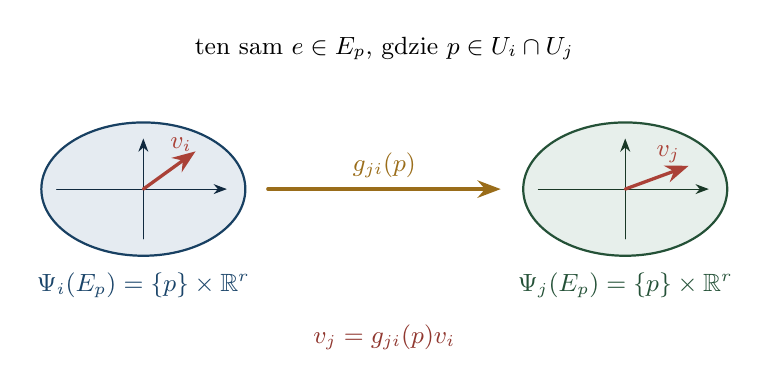
\begin{tikzpicture}[>=Stealth,scale=1.02,line cap=round]
\node[font=\small] at (0,1.75) {ten sam $e\in E_p$, gdzie $p\in U_i\cap U_j$};
\fill[manifoldblue!12] (-3,0) ellipse (1.27 and .83);
\draw[manifoldblue!70!black,thick] (-3,0) ellipse (1.27 and .83);
\draw[->,manifoldblue!45!black,thin] (-4.08,0)--(-1.96,0);
\draw[->,manifoldblue!45!black,thin] (-3,-.62)--(-3,.63);
\draw[->,manifoldred,very thick] (-3,0)--(-2.35,.47)
 node[pos=.72,above,font=\small] {$v_i$};
\fill[manifoldgreen!12] (3,0) ellipse (1.27 and .83);
\draw[manifoldgreen!65!black,thick] (3,0) ellipse (1.27 and .83);
\draw[->,manifoldgreen!45!black,thin] (1.92,0)--(4.04,0);
\draw[->,manifoldgreen!45!black,thin] (3,-.62)--(3,.63);
\draw[->,manifoldred,very thick] (3,0)--(3.79,.29)
 node[pos=.68,above,font=\small] {$v_j$};
\draw[->,very thick,manifoldgold!75!black] (-1.45,0)--(1.45,0)
 node[midway,above,font=\small] {$g_{ji}(p)$};
\node[font=\small,manifoldblue!75!black] at (-3,-1.2)
 {$\Psi_i(E_p)=\{p\}\times\R^r$};
\node[font=\small,manifoldgreen!65!black] at (3,-1.2)
 {$\Psi_j(E_p)=\{p\}\times\R^r$};
\node[font=\small\bfseries,manifoldred!85!black] at (0,-1.85)
 {$v_j=g_{ji}(p)v_i$};
\end{tikzpicture}
\caption{Dwie trywializacje tego samego włókna $E_p$. Wektor $e$ ma współrzędne $v_i$ i $v_j$, związane macierzą przejścia $g_{ji}(p)$.}
\end{figure}

\begin{uwaga}[Grupa strukturalna]
Wybór gładkich ram lokalnych daje funkcje o wartościach w
$\mathrm{GL}(r,\R)$; jest to
naturalna grupa strukturalna wiązki rzędu $r$. Jeżeli można dobrać
trywializacje tak, aby wszystkie macierze przejścia należały do podgrupy
$G\subseteq\mathrm{GL}(r,\R)$, mówimy o redukcji grupy strukturalnej do $G$.
Na przykład lokalne bazy ortonormalne wiązki z gładkim iloczynem
skalarnym we włóknach mają macierze przejścia w $\mathrm{O}(r)$.
W modelu wstęgi Möbiusa utożsamienie końców przedziału
zmienia znak współrzędnej włóknowej.
\end{uwaga}


\begin{przyklad}[Sekcje w zapisie lokalnym]
Niech $\pi:E\to M$ będzie wiązką wektorową rzędu $r$
z lokalnymi trywializacjami
$\Psi_i:E|_{U_i}\to U_i\times\R^r$ i funkcjami przejścia
$g_{ji}$.

Jeżeli $s:M\to E$ jest sekcją, to dla każdego $p\in U_i$
mamy $s(p)\in E_p$, a zatem $\Psi_i(s(p))=(p,s_i(p))$,
gdzie $s_i:U_i\to\R^r$ jest gładkim odwzorowaniem,
zwanym \emph{lokalnym zapisem sekcji} w trywializacji
$\Psi_i$.

Na przecięciu $U_i\cap U_j$ otrzymujemy
\[
\begin{aligned}
(p,s_j(p))
&=\Psi_j(s(p))\\
&=(\Psi_j\circ\Psi_i^{-1})(p,s_i(p))\\
&=(p,g_{ji}(p)s_i(p)),
\end{aligned}
\]
skąd $s_j(p)=g_{ji}(p)s_i(p)$.

Odwrotnie, jeżeli rodzina gładkich odwzorowań
$s_i:U_i\to\R^r$ spełnia powyższe warunki zgodności,
to wzór $s(p)=\Psi_i^{-1}(p,s_i(p)),\ p\in U_i$,
określa globalną sekcję wiązki $E$.
Istotnie, na przecięciu $U_i\cap U_j$ mamy
\[
\begin{aligned}
\Psi_j^{-1}(p,s_j(p))
&=\Psi_j^{-1}(p,g_{ji}(p)s_i(p))\\
&=\Psi_i^{-1}(p,s_i(p)),
\end{aligned}
\]
więc definicja nie zależy od wyboru indeksu.
Gładkość sekcji wynika z gładkości jej lokalnych
zapisów.

W szczególności, dla wiązki skonstruowanej przez
sklejanie z funkcji przejścia otrzymujemy $s(p)=[p,s_i(p)]_i$.

Rozważmy teraz wstęgę Möbiusa jako wiązkę liniową
nad okręgiem $S^1$. Możemy przedstawić ją jako
przestrzeń ilorazową $E=([0,2\pi]\times\R)/\sim$,
gdzie utożsamiamy $(0,v)\sim(2\pi,-v)$.
Rzutowanie na bazę jest dane wzorem $\pi([\theta,v])=e^{i\theta}$.

Sekcję opisujemy w tych współrzędnych za pomocą
funkcji $f:[0,2\pi]\to\R$, przypisując punktowi
$e^{i\theta}$ klasę $[\theta,f(\theta)]$.
Aby otrzymać dobrze określoną sekcję ciągłą,
funkcja $f$ musi być ciągła i spełniać $f(2\pi)=-f(0)$.
Dla sekcji gładkiej funkcja $f$ musi być gładka na domkniętym
przedziale i spełniać warunki zgodności wszystkich pochodnych
na utożsamianych końcach: $f^{(k)}(2\pi)=-f^{(k)}(0), \ k=0,1,2,\ldots$.

Pokażemy, że każda ciągła sekcja wstęgi Möbiusa
ma miejsce zerowe. Jeżeli $f(0)=0$, to teza
jest natychmiastowa. W przeciwnym razie
$f(2\pi)=-f(0)$ ma znak przeciwny do $f(0)$,
więc z twierdzenia o wartości pośredniej istnieje
$\theta_0\in(0,2\pi)$ takie, że $f(\theta_0)=0$.
Oznacza to, że $s(e^{i\theta_0})=0_{e^{i\theta_0}}$.

W szczególności wstęga Möbiusa nie posiada
globalnej sekcji nigdzie niezerowej, co stanowi
kolejny dowód jej nietrywialności jako wiązki
liniowej.
\end{przyklad}


\begin{definicja}[Suma i wiązka dualna]
\index{suma i wiazka dualna@Suma i wiązka dualna}
Dla wiązek $E,F$ nad tą samą bazą definiujemy włókna
$(E\oplus F)_p=E_p\oplus F_p$ oraz
$(E^*)_p=\mathrm{Hom}(E_p,\R)$. Przy macierzach przejścia $g_{ji}$
i $h_{ji}$ odpowiednie macierze to $g_{ji}\oplus h_{ji},\ (g_{ji}^{-1})^{\mathsf T}$.
Ostatni wzór wymusza zachowanie wartości funkcjonału:
jeżeli $v_j=g_{ji}v_i$ oraz $\xi_i(v_i)=\xi_j(v_j)$, to
$\xi_j=(g_{ji}^{-1})^{\mathsf T}\xi_i$. Obie rodziny spełniają
warunek kocyklu, więc twierdzenie o sklejaniu tworzy z nich wiązki.
\end{definicja}



\section{Różniczka, immersje, submersje i zanurzenia}

\begin{definicja}
Niech $F\colon M\to N$ będzie odwzorowaniem gładkim, $p\in M$. \emph{Różniczką} $F$ w
punkcie $p$ nazywamy odwzorowanie liniowe $dF_p\colon T_pM\to T_{F(p)}N$ zdefiniowane (w
języku derywacji) wzorem $(dF_p\,v)(g):=v(g\circ F), \ v\in T_pM,\ g\in C^\infty(N)$.

Równoważnie, jeśli $v=\gamma'(0)$ dla gładkiej krzywej
$\gamma\colon(-\varepsilon,\varepsilon)\to M$ z $\gamma(0)=p$, to $dF_p(v)=(F\circ\gamma)'(0)\in T_{F(p)}N$.
Istotnie, obie strony działają na $g\in C^\infty(N)$ jako
$(g\circ F\circ\gamma)'(0)=v(g\circ F)$. 
\end{definicja}

Jeśli krzywe $\gamma_1$ i
$\gamma_2$ mają tę samą prędkość $v$ w $p$, to dla każdego takiego $g$
obie prędkości $(F\circ\gamma_i)'(0)$ przyjmują na $g$ tę samą wartość
$v(g\circ F)$. Wektory styczne w $F(p)$ są derywacjami, więc są równe,
gdy działają jednakowo na wszystkie funkcje gładkie. Stąd wzór nie
zależy od wyboru krzywej reprezentującej $v$.
\begin{fakt}
$dF_pv$ jest istotnie derywacją w $F(p)$, a $dF_p$ jest odwzorowaniem liniowym.
\end{fakt}

\begin{proof}
Liniowość względem $g$: oczywista z liniowości $v$ i liniowości $g\mapsto g\circ F$.
Reguła Leibniza: $(dF_pv)(gh)=v((gh)\circ F)=v((g\circ F)(h\circ F))=(g\circ F)(p)\,
v(h\circ F)+(h\circ F)(p)\,v(g\circ F)=g(F(p))(dF_pv)(h)+h(F(p))(dF_pv)(g)$, na mocy reguły
Leibniza dla $v$ zastosowanej do $g\circ F,h\circ F\in C^\infty(M)$. Zatem $dF_pv\in
T_{F(p)}N$. Liniowość $dF_p$ względem $v$ jest natychmiastowa z liniowości $v\mapsto
v(g\circ F)$ w $v$, dla każdego ustalonego $g$.
\end{proof}

W Sekcji~\ref{sec:przestrzen-kostyczna} różniczkę funkcji
$f\colon M\to\R$ opisaliśmy jako kowektor $df_p\in T_p^*M$.
Powyższa definicja daje natomiast różniczkę odwzorowania
$f$ o wartościach w $T_{f(p)}\R$. Poniższy dowód utożsamia
te dwa opisy i wyjaśnia znany wzór na $df_p$ w mapie.



\begin{twierdzenie}[Różniczka odwzorowania we współrzędnych]
\label{tw:rozniczka-odwzorowania-wspolrzedne}
Niech $F\colon M\to N$ będzie odwzorowaniem gładkim, gdzie
$\dim M=m$ i $\dim N=n$. Niech $(U,\varphi)$ będzie mapą
wokół $p$, o współrzędnych $(x^1,\ldots,x^m)$, a $(V,\psi)$
mapą wokół $F(p)$, o współrzędnych $(y^1,\ldots,y^n)$.
Zmniejszając w razie potrzeby $U$, zakładamy, że
$F(U)\subset V$, i oznaczamy
\[
\widehat F:=\psi\circ F\circ\varphi^{-1}
=(\widehat F^{\,1},\ldots,\widehat F^{\,n}).
\]
Wówczas dla każdego $v\in T_pM$ zachodzi
\[
dF_p(v)=
\sum_{j=1}^n\sum_{i=1}^m
\frac{\partial\widehat F^{\,j}}{\partial u^i}
\bigl(\varphi(p)\bigr)\,dx_p^i(v)
\left.\frac{\partial}{\partial y^j}\right|_{F(p)}.
\]
W szczególności macierzą różniczki $dF_p$ w bazach
współrzędnościowych jest macierz Jacobiego
\[
[dF_p]=D\widehat F(\varphi(p))
=
\left[
\frac{\partial\widehat F^{\,j}}{\partial u^i}
\bigl(\varphi(p)\bigr)
\right]_{\substack{1\le j\le n\\1\le i\le m}}.
\]
\emph{Rzędem} odwzorowania $F$ w punkcie $p$ nazywamy
rząd $dF_p$, równy rzędowi powyższej macierzy.
\end{twierdzenie}

\begin{proof}
Z dualności baz współrzędnościowych mamy
\[
dx_p^i\left(
\left.\frac{\partial}{\partial x^j}\right|_p
\right)=\delta_j^i.
\]
Każdy wektor $v\in T_pM$ można zapisać jako
\[
v=\sum_{i=1}^m v^i
\left.\frac{\partial}{\partial x^i}\right|_p.
\]
Stosując $dx_p^j$ do obu stron, otrzymujemy
$v^j=dx_p^j(v)$, a zatem
\[
v=\sum_{i=1}^m dx_p^i(v)
\left.\frac{\partial}{\partial x^i}\right|_p.
\]

Niech $g$ będzie funkcją gładką określoną w otoczeniu
$F(p)$. Można ją przedłużyć funkcją odcinającą do funkcji
na $N$; wynik nie zależy od przedłużenia dzięki
Lematowi~\ref{lem:lokalnosc}. Dotyczy to również
lokalnych funkcji współrzędnych $y^j$ użytych poniżej.
Z definicji różniczki oraz powyższego rozkładu
wynika
\[
\begin{aligned}
(dF_p(v))(g)
&=v(g\circ F)\\
&=\sum_{i=1}^m dx_p^i(v)
\left.\frac{\partial}{\partial x^i}\right|_p(g\circ F)\\
&=\sum_{i=1}^m dx_p^i(v)
\frac{\partial(g\circ F\circ\varphi^{-1})}
{\partial u^i}\bigl(\varphi(p)\bigr).
\end{aligned}
\]

Aby wyznaczyć współrzędne wektora $dF_p(v)$,
stosujemy go do funkcji współrzędnych $y^j$.
Istotnie, z dualności baz w $T_{F(p)}N$ mamy
\[
w=\sum_{j=1}^n dy_{F(p)}^j(w)
\left.\frac{\partial}{\partial y^j}\right|_{F(p)},
\qquad
dy_{F(p)}^j(w)=w(y^j).
\]
Podstawiając $g=y^j$ i korzystając z równości
$\widehat F^{\,j}=y^j\circ F\circ\varphi^{-1}$,
otrzymujemy
\[
\begin{aligned}
dy_{F(p)}^j(dF_p(v))
&=(dF_p(v))(y^j)\\
&=\sum_{i=1}^m dx_p^i(v)
\frac{\partial\widehat F^{\,j}}{\partial u^i}
\bigl(\varphi(p)\bigr).
\end{aligned}
\]
Wstawiając te współczynniki do rozkładu wektora
$dF_p(v)$ w bazie współrzędnościowej, otrzymujemy
żądaną postać różniczki.

W szczególności, dla
$v=\partial/\partial x^i|_p$ mamy
\[
dF_p\left(
\left.\frac{\partial}{\partial x^i}\right|_p
\right)
=
\sum_{j=1}^n
\frac{\partial\widehat F^{\,j}}{\partial u^i}
\bigl(\varphi(p)\bigr)
\left.\frac{\partial}{\partial y^j}\right|_{F(p)}.
\]
Współczynniki przy wektorach bazy docelowej
tworzą kolejne kolumny macierzy $dF_p$,
czyli macierz Jacobiego $D\widehat F(\varphi(p))$.
\end{proof}

\begin{wniosek}[Różniczka funkcji we współrzędnych]
\label{tw:rozniczka-funkcji-wspolrzedne}
Niech $f\colon M\to\R$ będzie funkcją gładką,
a $(U,\varphi)$ mapą wokół $p$, o współrzędnych
$(x^1,\ldots,x^m)$. Oznaczmy
\[
\widehat f:=f\circ\varphi^{-1}.
\]
Po standardowym utożsamieniu $T_{f(p)}\R$ z $\R$
różniczka $df_p$ jest kowektorem i ma postać
\begin{equation}
\label{eq:df-wspolrzedne}
df_p=\sum_{i=1}^m
\frac{\partial f}{\partial x^i}(p)\,dx_p^i,
\qquad
\frac{\partial f}{\partial x^i}(p)
:=
\frac{\partial\widehat f}{\partial u^i}
\bigl(\varphi(p)\bigr).
\end{equation}
W szczególności, jeśli
$v=\sum_i v^i\partial/\partial x^i|_p$, to
\[
df_p(v)=\sum_{i=1}^m
v^i\frac{\partial f}{\partial x^i}(p).
\]
\end{wniosek}

\begin{proof}
Niech $t\colon\R\to\R$ będzie standardową
współrzędną, czyli $t(a)=a$. Każdy wektor
$w\in T_{f(p)}\R$ ma jednoznaczną postać
\[
w=a\left.\frac{\partial}{\partial t}\right|_{f(p)},
\qquad a\in\R.
\]
Standardowy izomorfizm $T_{f(p)}\R\cong\R$
przyporządkowuje temu wektorowi liczbę $a$.
Ponieważ
\[
\left.\frac{\partial}{\partial t}\right|_{f(p)}(t)=1,
\]
współczynnik ten możemy odczytać jako $a=w(t)$.
Zatem utożsamienie ma postać
\[
T_{f(p)}\R\longrightarrow\R,
\qquad w\longmapsto w(t).
\]

W szczególności różniczka odwzorowania
$f$, która pierwotnie przyjmuje wartości
w $T_{f(p)}\R$, po tym utożsamieniu spełnia
\[
df_p(v)=(df_p(v))(t)
=v(t\circ f)=v(f).
\]
Pierwsza równość oznacza tutaj zastosowanie
powyższego izomorfizmu, a druga wynika
z definicji różniczki odwzorowania.

Ponieważ lokalną reprezentacją $f$ względem
standardowej współrzędnej $t$ jest
$\widehat f=f\circ\varphi^{-1}$, poprzednie
twierdzenie daje
\[
df_p(v)=
\sum_{i=1}^m
\frac{\partial\widehat f}{\partial u^i}
\bigl(\varphi(p)\bigr)\,dx_p^i(v).
\]
Ponieważ równość zachodzi dla każdego
$v\in T_pM$, otrzymujemy wzór
\eqref{eq:df-wspolrzedne}.
\end{proof}

Na przykład dla $f(u,v)=u^2+uv$ na $\R^2$ mamy
$\partial_u f=2u+v$ i $\partial_v f=u$, więc
\[
 df_{(u,v)}=(2u+v)\,du_{(u,v)}+u\,dv_{(u,v)}.
\]
W punkcie $(1,2)$ dostajemy $df_{(1,2)}=4\,du_{(1,2)}+dv_{(1,2)}$;
na wektorze $a\,\partial_u|_{(1,2)}+b\,\partial_v|_{(1,2)}$
różniczka ma wartość $4a+b$.

\begin{twierdzenie}[Reguła łańcucha]
Jeśli $F\colon M\to N$ i $G\colon N\to P$ są gładkie, $p\in M$, to
$d(G\circ F)_p=dG_{F(p)}\circ dF_p\colon T_pM\to T_{G(F(p))}P$.
\end{twierdzenie}
\begin{proof}
Dla $v\in T_pM$ i $h\in C^\infty(P)$, z definicji różniczki:
\[
\big(d(G\circ F)_p\,v\big)(h)=v\big(h\circ(G\circ F)\big)=v\big((h\circ G)\circ F\big)=
(dF_pv)(h\circ G)=\big(dG_{F(p)}(dF_pv)\big)(h),
\]
gdzie w trzeciej równości zastosowaliśmy definicję $dF_p$ do $h\circ G\in C^\infty(N)$, a
w czwartej — definicję $dG_{F(p)}$ do $dF_pv\in T_{F(p)}N$. Zatem $d(G\circ F)_pv=
dG_{F(p)}(dF_pv)$ dla każdego $v$ — co dowodzi tezy.
\end{proof}


\begin{definicja}
Niech $F\colon M\to N$ będzie gładkie, $\dim M=m$, $\dim N=n$. Mówimy, że $F$ jest w
punkcie $p$ \emph{immersją}, jeśli $dF_p$ jest injektywne, oraz \emph{submersją}, jeśli
$dF_p$ jest surjektywne. $F$ jest immersją (submersją), jeśli jest nią w każdym punkcie
$p\in M$. \emph{Zanurzeniem} (ang.\ \emph{embedding}) nazywamy immersję $F\colon M\to N$,
która dodatkowo jest homeomorfizmem na obraz $F(M)$ (z topologią podprzestrzeni $N$).
\end{definicja}

Poniższy przykład pokazuje, że sama różnowartościowa immersja nie musi być zanurzeniem —
warunek ,,homeomorfizm na obraz'' jest istotnie mocniejszy.

\begin{przyklad}[Krzywa ósemkowa]\label{prz:osemka}
Niech $\beta\colon(-\pi,\pi)\to\R^2$, $\beta(t):=(\sin2t,\ \sin t)$.

\emph{$\beta$ jest immersją.} $\beta'(t)=(2\cos2t,\cos t)$. Gdyby $\beta'(t_0)=0$, to
$\cos t_0=0$ (więc $t_0=\pm\pi/2$) oraz $\cos2t_0=0$; ale $\cos(\pm\pi)=-1\neq0$ —
sprzeczność. Zatem $\beta'(t)\neq0$ dla wszystkich $t$, czyli $d\beta_t$ jest injektywne w
każdym punkcie.

\emph{$\beta$ jest różnowartościowa.} Przypuśćmy $\beta(t_1)=\beta(t_2)$, tzn.\ $\sin t_1=
\sin t_2=:s$ oraz $\sin2t_1=\sin2t_2$. Jeśli $s=0$: na $(-\pi,\pi)$ równość $\sin t=0$
zachodzi jedynie dla $t=0$, więc $t_1=t_2=0$. Jeśli $s\neq0$: korzystając z $\sin2t_i=
2\sin t_i\cos t_i=2s\cos t_i$, równość $\sin2t_1=\sin2t_2$ daje (dzieląc przez $2s\neq0$)
$\cos t_1=\cos t_2$. Zatem $\sin t_1=\sin t_2$ i $\cos t_1=\cos t_2$ jednocześnie — co
oznacza $t_1-t_2\in2\pi\Z$; ponieważ $t_1,t_2\in(-\pi,\pi)$, jedyna możliwość to $t_1=t_2$.
W obu przypadkach $\beta$ jest różnowartościowa.

\emph{$\beta$ nie jest zanurzeniem.} $\lim_{t\to\pi^-}\beta(t)=(\sin2\pi,\sin\pi)=(0,0)$
oraz $\lim_{t\to-\pi^+}\beta(t)=(0,0)$ — oba końce krzywej zbiegają do tego samego punktu
$(0,0)=\beta(0)$. Odwzorowanie odwrotne $\beta^{-1}$ nie jest więc ciągłe w $(0,0)$: dla
ciągu $t_k\to\pi^-$, $\beta(t_k)\to(0,0)=\beta(0)$, ale $\beta^{-1}(\beta(t_k))=t_k\to\pi
\neq0=\beta^{-1}(0,0)$. Zatem $\beta$ jest różnowartościową immersją, która nie jest
homeomorfizmem na obraz — nie jest zanurzeniem.
\end{przyklad}

\begin{figure}[h]
\centering
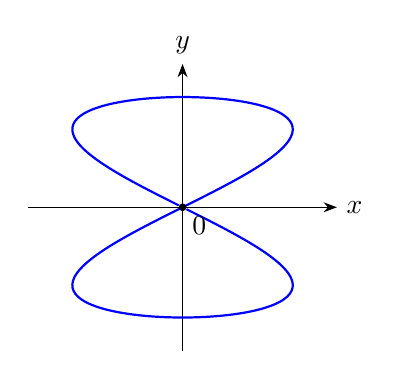
\begin{tikzpicture}[>=Stealth,scale=1.4]
\draw[->] (-1.4,0) -- (1.4,0) node[right]{$x$};
\draw[->] (0,-1.3) -- (0,1.3) node[above]{$y$};
\draw[thick,blue,domain=-179:179,samples=150,smooth]
plot ({sin(2*\x)},{sin(\x)});
\fill (0,0) circle (1pt) node[below right]{$0$};
\end{tikzpicture}
\caption{Krzywa ósemkowa $\beta(t)=(\sin2t,\sin t)$: różnowartościowa immersja, która nie
jest zanurzeniem — oba końce ($t\to\pm\pi$) zbiegają do początku układu współrzędnych.}
\label{fig:osemka}
\end{figure}


\begin{uwaga}[Nawinięcie niewymierne torusa]
Podobny, choć bardziej subtelny, przykład daje
\emph{nawinięcie niewymierne} torusa
$T^2=\R^2/\Z^2$. Rozważmy odwzorowanie $\gamma:\R\longrightarrow T^2, \ \gamma(t)=(t,\alpha t)+\Z^2$,
gdzie $\alpha\in\R\setminus\Q$.

Pokażemy, że $\gamma$ jest injektywną immersją,
która nie jest zanurzeniem, a jej obraz
jest gęsty w $T^2$.

\smallskip
\noindent\textbf{Injektywność i immersyjność.}
Jeżeli $\gamma(t)=\gamma(s)$, to $(t-s,\alpha(t-s))\in\Z^2$.
W szczególności $t-s\in\Z$ oraz
$\alpha(t-s)\in\Z$. Gdyby $t-s\ne0$,
otrzymalibyśmy $\alpha=\frac{\alpha(t-s)}{t-s}\in\Q$,
co przeczy niewymierności $\alpha$.
Zatem $t=s$, czyli $\gamma$ jest injektywna.

Ponieważ rzutowanie $\R^2\to T^2$ jest lokalnym
dyfeomorfizmem, różniczka $\gamma$ jest lokalnie
reprezentowana przez wektor $\gamma'(t)=(1,\alpha)\ne(0,0)$.
Ma więc rząd $1$ w każdym punkcie, co dowodzi,
że $\gamma$ jest immersją.

\smallskip
\noindent\textbf{Nieciągłość odwrotności na obraz.}
Wykażemy, że istnieje ciąg liczb całkowitych
dodatnich $q_N\to\infty$ taki, że $\gamma(q_N)\longrightarrow\gamma(0)$.

W tym celu ustalmy $N\ge1$ i podzielmy przedział
$[0,1)$ na $N$ rozłącznych przedziałów $I_j=\left[\frac{j}{N},\frac{j+1}{N}\right), \ j=0,\ldots,N-1$.
Każdy z nich ma długość $1/N$.

Rozważmy teraz $N+1$ liczb $\{0\alpha\},\{\alpha\},\{2\alpha\}, \ldots,\{N\alpha\}\in[0,1)$,
gdzie $\{x\}:=x-\lfloor x\rfloor$ oznacza
część ułamkową liczby $x$.

Ponieważ mamy $N+1$ liczb i tylko $N$
przedziałów, z zasady szufladkowej istnieją
indeksy $0\le k<l\le N$ takie, że
$\{k\alpha\}$ i $\{l\alpha\}$ należą do
tego samego przedziału $I_j$.

Wobec tego $|\{l\alpha\}-\{k\alpha\}|<\frac1N$.
Korzystając z definicji części ułamkowej,
otrzymujemy
\[
\left|
(l-k)\alpha-
\bigl(\lfloor l\alpha\rfloor
-\lfloor k\alpha\rfloor\bigr)
\right|<\frac1N.
\]
Oznaczając $q_N:=l-k,\ p_N:=\lfloor l\alpha\rfloor -\lfloor k\alpha\rfloor$,
dostajemy $1\le q_N\le N,\ p_N\in\Z, \ |q_N\alpha-p_N|<\frac1N$.

Pokażemy, że $q_N\to\infty$.
Gdyby tak nie było, istniałyby liczba
naturalna $K$ oraz nieskończenie wiele
indeksów $N$, dla których $q_N\le K$.
Ponieważ $\alpha$ jest niewymierna,
żadna z liczb $q\alpha$, $1\le q\le K$,
nie jest całkowita. Zatem $\delta_K:= \min_{1\le q\le K} \operatorname{dist}(q\alpha,\Z)>0$.
Jednak dla wspomnianych indeksów $N$ mamy $\delta_K \le |q_N\alpha-p_N| <\frac1N$,
co dla dostatecznie dużego $N$ prowadzi
do sprzeczności. Stąd $q_N\to\infty$.

Z drugiej strony, ponieważ $q_N,p_N\in\Z$,
w torusie zachodzi
\[
\begin{aligned}
\gamma(q_N)
&=(q_N,\alpha q_N)+\Z^2\\
&=(0,\alpha q_N-p_N)+\Z^2.
\end{aligned}
\]
Ponieważ $|\alpha q_N-p_N|<1/N$, otrzymujemy $\gamma(q_N)\longrightarrow(0,0)+\Z^2 =\gamma(0)$.

Przypuśćmy teraz, że odwrotność $\gamma^{-1}:\gamma(\R)\longrightarrow\R$
jest ciągła, przy czym $\gamma(\R)$
wyposażamy w topologię podprzestrzeni
odziedziczoną z $T^2$.

Z ciągłości $\gamma^{-1}$ w punkcie
$\gamma(0)$ oraz ze zbieżności
$\gamma(q_N)\to\gamma(0)$ wynikałoby
\[
q_N
=\gamma^{-1}(\gamma(q_N))
\longrightarrow
\gamma^{-1}(\gamma(0))=0.
\]
Jest to sprzeczne z $q_N\to\infty$.

Zatem $\gamma^{-1}$ nie jest ciągła,
a więc $\gamma$ nie jest homeomorfizmem
na swój obraz. W szczególności nie jest
zanurzeniem.

\smallskip
\noindent\textbf{Gęstość obrazu.}
Pokażemy jeszcze, że $\gamma(\R)$ jest
gęsty w $T^2$.

Najpierw udowodnimy, że zbiór $\{k\alpha+\Z:k\in\Z\}$
jest gęsty w okręgu $\R/\Z$.

Niech $\varepsilon\in(0,1)$.
Z wykazanego wyżej przybliżenia wynika,
że istnieją $q\in\N$ i $p\in\Z$ takie, że $0<|q\alpha-p|<\varepsilon$.
Oznaczmy $\delta:=q\alpha-p$ oraz
$d:=|\delta|$. Mamy więc $0<d<\varepsilon$.

Rozważmy punkty $0,d,2d,\ldots,\left\lfloor\frac1d\right\rfloor d$
w przedziale $[0,1]$.
Odległości między kolejnymi punktami
wynoszą $d$, natomiast odległość ostatniego
punktu od $1$ jest mniejsza niż $d$.
Zatem każdy punkt przedziału $[0,1]$
znajduje się w odległości mniejszej niż
$\varepsilon$ od jednego z tych punktów.

Ponadto każda wielokrotność $nd$ jest,
modulo $\Z$, całkowitą wielokrotnością
$\alpha$, gdyż $nd=n|q\alpha-p| \equiv \operatorname{sgn}(\delta)nq\alpha \pmod{\Z}$.
Wobec tego całkowite wielokrotności
$\alpha$ są $\varepsilon$-gęste
w $\R/\Z$. Ponieważ $\varepsilon>0$
było dowolne, otrzymujemy żądaną gęstość.

Niech teraz $(a,b)+\Z^2$ będzie dowolnym
punktem torusa. Z wykazanej gęstości
możemy dla dowolnego $\varepsilon>0$
wybrać $k\in\Z$ tak, aby $\operatorname{dist} \bigl(\alpha k-(b-\alpha a),\Z\bigr) <\varepsilon$.
Wtedy
\[
\begin{aligned}
\gamma(a+k)
&=(a+k,\alpha a+\alpha k)+\Z^2\\
&=(a,\alpha a+\alpha k)+\Z^2,
\end{aligned}
\]
a druga współrzędna tego punktu jest,
modulo $\Z$, odległa od $b$ o mniej
niż $\varepsilon$.

Ponieważ pierwsza współrzędna jest
dokładnie równa $a$ modulo $\Z$,
punkt $\gamma(a+k)$ może leżeć
dowolnie blisko $(a,b)+\Z^2$.
Stąd $\overline{\gamma(\R)}=T^2$.
\end{uwaga}


\subsection*{Twierdzenie o rzędzie stałym}

\begin{lemat}[Półciągłość rzędu z dołu]\label{lem:polciaglosc}
Niech $F\colon M\to N$ będzie gładkie. Zbiór $\{p\in M:\mathrm{rz}(dF_p)\geq r\}$ jest
otwarty w $M$, dla każdego $r$.
\end{lemat}
\begin{proof}
Warunek $\mathrm{rz}(dF_p)\geq r$ oznacza, w mapach lokalnych, że macierz Jacobiego $DF$ w
$\varphi(p)$ ma pewien minor stopnia $r$ różny od zera. Wyznacznik danego minora jest
funkcją ciągłą (wielomianem od wyrazów macierzy Jacobiego, gładkich funkcji punktu), więc
zbiór punktów, w których ten minor jest niezerowy, jest otwarty. Zbiór $\{\mathrm{rz}
(dF_p)\geq r\}$ jest sumą (po wszystkich wyborach minora stopnia $r$) takich zbiorów
otwartych, a więc otwarty.
\end{proof}

\begin{wniosek}\label{wn:stalyrzad}
Jeśli $F\colon M\to N$ jest immersją (submersją) w punkcie $p$, to $F$ jest immersją
(submersją) na pewnym otoczeniu $p$, o \emph{stałym} rzędzie na tym otoczeniu.
\end{wniosek}
\begin{proof}
Niech $m=\dim M$, $n=\dim N$. Jeśli $F$ jest immersją w $p$, $\mathrm{rz}(dF_p)=m$; ale
rząd $dF_q\colon\R^m\to\R^n$ jest zawsze $\leq m$, więc z Lematu~\ref{lem:polciaglosc}
($r=m$), $\{\mathrm{rz}(dF_q)\geq m\}=\{\mathrm{rz}(dF_q)=m\}$ jest otoczeniem otwartym
$p$, na którym $F$ ma stały rząd $m$. Przypadek submersji jest analogiczny z $r=n$.
\end{proof}

\begin{twierdzenie}[Twierdzenie o rzędzie stałym]
\label{tw:rzad-staly}
Niech $F\colon M\to N$
będzie odwzorowaniem gładkim o stałym rzędzie $k$ na pewnym otoczeniu
punktu $p\in M$, gdzie $\dim M=m, \ \dim N=n$.
Wówczas istnieją mapy $(U,\varphi) \ \text{oraz}\ (V,\psi)$
wokół odpowiednio $p$ i $F(p)$, takie że $\varphi(p)=0, \ \psi(F(p))=0, \ F(U)\subseteq V$,
oraz
\[
(\psi\circ F\circ\varphi^{-1})(u^1,\dots,u^m)
=
(u^1,\dots,u^k,0,\dots,0).
\]
\end{twierdzenie}
\begin{proof}
Wybierzmy najpierw dowolne mapy
\[
\varphi_0\colon U_0\to\varphi_0(U_0)\subset\R^m, \qquad \psi_0\colon V_0\to\psi_0(V_0)\subset\R^n
\]
wokół odpowiednio punktów $p$ i $F(p)$, takie że $\varphi_0(p)=0, \ \psi_0(F(p))=0$.
Po ewentualnym zmniejszeniu $U_0$ możemy założyć, że $F(U_0)\subseteq V_0$
oraz że $F$ ma stały rząd $k$ na całym $U_0$.

W tych mapach odwzorowanie $F$ jest reprezentowane przez gładkie
odwzorowanie
\[
\widehat F := \psi_0\circ F\circ\varphi_0^{-1} \colon \varphi_0(U_0)\longrightarrow\psi_0(V_0).
\]
Ponieważ $\varphi_0(p)=0 \ \text{oraz}\ \psi_0(F(p))=0$,
mamy $\widehat F(0)=0$.

Pokażmy najpierw, że $\widehat F$ ma ten sam rząd co $F$.
Niech $q\in U_0, \ u:=\varphi_0(q)$.
Z reguły łańcuchowej otrzymujemy
\[
D\widehat F_u = D(\psi_0)_{F(q)} \circ \dd F_q \circ D(\varphi_0^{-1})_u.
\]
Ponieważ $\varphi_0$ i $\psi_0$ są mapami, odwzorowania $D(\psi_0)_{F(q)} \ \text{oraz}\ D(\varphi_0^{-1})_u$
są izomorfizmami liniowymi. Złożenie odwzorowania liniowego
z izomorfizmami po lewej i prawej stronie nie zmienia jego rzędu,
a zatem $\operatorname{rz}(D\widehat F_u) = \operatorname{rz}(\dd F_q) = k$.
Odwzorowanie $\widehat F$ ma więc stały rząd $k$ na rozważanym
otoczeniu zera.

Dalszą część dowodu przeprowadzimy dla $\widehat F$ pomiędzy
otwartymi podzbiorami przestrzeni euklidesowych, a na końcu
przeniesiemy skonstruowane współrzędne z powrotem na rozmaitości.

\medskip
\emph{Przypadek $k=0$.}

Jeżeli $k=0$, to $D\widehat F_u=0$
dla każdego $u$ w dostatecznie małym otoczeniu zera.
Zmniejszając to otoczenie, możemy założyć, że jest ono wypukłe.

Dla ustalonego $u$ rozważmy krzywą $\gamma(t):=\widehat F(tu), \ 0\leq t\leq1$.
Z reguły łańcuchowej $\gamma'(t) = D\widehat F_{tu}(u) = 0$.
Krzywa $\gamma$ jest więc stała, a zatem $\widehat F(u) = \widehat F(0) = 0$.
Wobec tego $\widehat F(u)=(0,\dots,0)$,
czyli $\widehat F$ ma już żądaną postać normalną.

Po odpowiednim zmniejszeniu dziedzin możemy więc przyjąć $\varphi=\varphi_0, \ \psi=\psi_0$,
co kończy dowód w przypadku $k=0$.

Dalej zakładamy, że $k>0$.

\medskip
\emph{Krok 1: wybór odpowiednich współrzędnych i pierwszy
dyfeomorfizm lokalny.}

Ponieważ $\operatorname{rz}(D\widehat F(0))=k$,
istnieje niezerowy minor stopnia $k$ macierzy $D\widehat F(0)$.
Po odpowiednim przenumerowaniu współrzędnych w $\R^m$ oraz $\R^n$
możemy założyć, że jest to minor utworzony z pierwszych $k$
wierszy i pierwszych $k$ kolumn.

Formalnie takie przenumerowanie odpowiada złożeniu map
$\varphi_0$ i $\psi_0$ z odpowiednimi liniowymi izomorfizmami
będącymi permutacjami współrzędnych. Aby nie komplikować notacji,
otrzymane w ten sposób mapy nadal oznaczamy przez
$\varphi_0$ i $\psi_0$, a odpowiadającą im reprezentację $F$
przez $\widehat F$.

Piszemy $\widehat F = (\widehat F^1,\dots,\widehat F^n)$.
Macierz
\[
A := \left( \frac{\partial\widehat F^i}{\partial u^j}(0) \right)_{1\leq i,j\leq k}
\]
jest zatem odwracalna.

Definiujemy odwzorowanie $\Phi\colon\varphi_0(U_0)\to\R^m$
wzorem
\[
\Phi(u) := \bigl( \widehat F^1(u),\dots,\widehat F^k(u), u^{k+1},\dots,u^m \bigr).
\]
Macierz jego różniczki w zerze ma postać blokową
\[
D\Phi(0)
=
\begin{pmatrix}
A&B\\
0&I_{m-k}
\end{pmatrix}.
\]
Blok zerowy w lewym dolnym rogu pojawia się dlatego, że ostatnie
$m-k$ składowych $\Phi$ są funkcjami $u^{k+1},\dots,u^m$
i nie zależą od $u^1,\dots,u^k$.

Ponieważ macierz jest blokowo trójkątna, $\det D\Phi(0) = \det A\neq0$.
Na mocy twierdzenia o odwzorowaniu odwrotnym istnieje otwarte
otoczenie $W$ punktu $0$ takie, że $\Phi\colon W\longrightarrow\Phi(W)$
jest dyfeomorfizmem.

Po dalszym zmniejszeniu $U_0$ możemy zakładać, że $\varphi_0(U_0)\subseteq W$.

\medskip
\emph{Krok 2: przepisanie $\widehat F$ w nowych współrzędnych
dziedziny.}

Definiujemy $G := \widehat F\circ\Phi^{-1}$.
Niech $w=\Phi(u)$.
Z definicji $\Phi$ mamy $w^i=\widehat F^i(u), \ i=1,\dots,k$.
Ponieważ $G(w) = \widehat F(\Phi^{-1}(w)) = \widehat F(u)$,
otrzymujemy $G^i(w)=w^i, \ i=1,\dots,k$.

Dla pozostałych składowych wprowadzamy oznaczenie $h^i(w):=G^i(w), \ i=k+1,\dots,n$.
Wobec tego $G(w) = \bigl( w^1,\dots,w^k, h^{k+1}(w),\dots,h^n(w) \bigr)$.

\medskip
\emph{Krok 3: funkcje $h^i$ zależą tylko od
$w^1,\dots,w^k$.}

Ponieważ $G=\widehat F\circ\Phi^{-1}$,
a $\Phi^{-1}$ jest lokalnym dyfeomorfizmem, $G$ ma ten sam
stały rząd co $\widehat F$, czyli $\operatorname{rz}(DG(w))=k$.

Macierz różniczki $G$ ma postać
\[
DG(w)
=
\begin{pmatrix}
I_k&0\\
*&
\left(
\frac{\partial h^i}{\partial w^j}(w)
\right)_{\substack{i=k+1,\dots,n\\ j=k+1,\dots,m}}
\end{pmatrix}.
\]

Przypuśćmy, że dla pewnych $i_0>k, \ j_0>k$
oraz pewnego punktu $w_0$ zachodzi $\frac{\partial h^{i_0}}{\partial w^{j_0}}(w_0)\neq0$.
Rozważmy minor stopnia $k+1$ macierzy $DG(w_0)$ utworzony
z wierszy $1,\dots,k,i_0$
oraz kolumn $1,\dots,k,j_0$.
Odpowiadająca mu macierz ma postać
\[
\begin{pmatrix}
I_k&0\\
*&
\dfrac{\partial h^{i_0}}{\partial w^{j_0}}(w_0)
\end{pmatrix},
\]
więc jej wyznacznik wynosi $\frac{\partial h^{i_0}}{\partial w^{j_0}}(w_0)\neq0$.
Oznaczałoby to $\operatorname{rz}(DG(w_0))\geq k+1$,
co przeczy założeniu, że $G$ ma stały rząd $k$.

Zatem
\[
\frac{\partial h^i}{\partial w^j}=0
\qquad
\text{dla wszystkich }i>k,\ j>k.
\]

Zmniejszmy teraz dziedzinę $G$ tak, aby zawierała produkt
otwartych kul $A\times B \subset \R^k\times\R^{m-k}$
o środku $0$. Piszemy $w=(a,b), \ a=(w^1,\dots,w^k), \ b=(w^{k+1},\dots,w^m)$.
Dla $(a,b)\in A\times B$ oraz $i>k$ mamy
\begin{align*}
h^i(a,b)-h^i(a,0)
&=
\int_0^1
\frac{d}{dt}h^i(a,tb)\,dt\\
&=
\int_0^1
\sum_{j=k+1}^m
b^j
\frac{\partial h^i}{\partial w^j}(a,tb)\,dt\\
&=
0.
\end{align*}
Zatem $h^i(a,b)=h^i(a,0)$.
Każda funkcja $h^i$ zależy więc jedynie od pierwszych $k$
współrzędnych. Dalej będziemy pisać po prostu $h^i(w^1,\dots,w^k)$
zamiast $h^i(w^1,\dots,w^k,0,\dots,0)$.

W konsekwencji
\[
G(w) = \bigl( w^1,\dots,w^k, h^{k+1}(w^1,\dots,w^k), \dots, h^n(w^1,\dots,w^k) \bigr).
\]

\medskip
\emph{Krok 4: zmiana współrzędnych w przestrzeni docelowej.}

Na dostatecznie małym otwartym otoczeniu zera w $\R^n$
definiujemy
\[
\Psi(y^1,\dots,y^n)
:=
\bigl(
y^1,\dots,y^k,
y^{k+1}-h^{k+1}(y^1,\dots,y^k),
\dots,
y^n-h^n(y^1,\dots,y^k)
\bigr).
\]
Odwzorowanie to ma jawną odwrotność
\[
\Psi^{-1}(z^1,\dots,z^n)
=
\bigl(
z^1,\dots,z^k,
z^{k+1}+h^{k+1}(z^1,\dots,z^k),
\dots,
z^n+h^n(z^1,\dots,z^k)
\bigr).
\]
Bezpośrednie podstawienie pokazuje, że
\[
\Psi^{-1}\circ\Psi=\operatorname{id}
\qquad\text{oraz}\qquad
\Psi\circ\Psi^{-1}=\operatorname{id}.
\]
Odwzorowania $\Psi$ i $\Psi^{-1}$ są gładkie, zatem $\Psi$
jest dyfeomorfizmem swojego otwartego obszaru definicji na obraz.

Dla $w$ dostatecznie bliskiego $0$ mamy
\[
G(w) = \bigl( w^1,\dots,w^k, h^{k+1}(w^1,\dots,w^k), \dots, h^n(w^1,\dots,w^k) \bigr),
\]
a zatem
\begin{align*}
(\Psi\circ G)(w)
&=
\Psi\bigl(
w^1,\dots,w^k,
h^{k+1}(w^1,\dots,w^k),
\dots,
h^n(w^1,\dots,w^k)
\bigr)\\
&=
(w^1,\dots,w^k,0,\dots,0).
\end{align*}
Otrzymaliśmy więc w przestrzeniach euklidesowych postać normalną
\[
\Psi\circ\widehat F\circ\Phi^{-1}
= (w^1,\dots,w^k,0,\dots,0).
\]

\medskip
\emph{Krok 5: powrót do map na rozmaitościach.}

Pozostaje przełożyć skonstruowane powyżej zmiany współrzędnych
na nowe mapy rozmaitości $M$ i $N$.

Przypomnijmy, że początkowa reprezentacja $F$ miała postać $\widehat F = \psi_0\circ F\circ\varphi_0^{-1}$.
Odwzorowanie $\Phi$ jest zmianą współrzędnych po stronie dziedziny,
natomiast $\Psi$ jest zmianą współrzędnych po stronie przeciwdziedziny.

Definiujemy zatem nowe mapy przez
\[
\boxed{ \varphi:=\Phi\circ\varphi_0 }
\]
oraz
\[
\boxed{ \psi:=\Psi\circ\psi_0. }
\]
Po odpowiednim zmniejszeniu $U_0$ oraz $V_0$ są to mapy
\[
\varphi\colon U\to\varphi(U)\subset\R^m, \qquad \psi\colon V\to\psi(V)\subset\R^n
\]
wokół odpowiednio $p$ i $F(p)$.

Sprawdźmy najpierw położenie wyróżnionych punktów. Ponieważ $\varphi_0(p)=0$
oraz $\widehat F(0)=0$,
z definicji $\Phi$ otrzymujemy
\[
\Phi(0) = \bigl( \widehat F^1(0),\dots,\widehat F^k(0), 0,\dots,0 \bigr) = 0.
\]
Stąd $\varphi(p) = \Phi(\varphi_0(p)) = \Phi(0) = 0$.

Ponadto $G(0) = \widehat F(\Phi^{-1}(0)) = \widehat F(0) = 0$.
Ponieważ $G(0) = \bigl( 0,\dots,0, h^{k+1}(0),\dots,h^n(0) \bigr)$,
wynika stąd $h^{k+1}(0)=\cdots=h^n(0)=0$.
Z definicji $\Psi$ otrzymujemy więc $\Psi(0)=0$.
Wobec tego $\psi(F(p)) = \Psi(\psi_0(F(p))) = \Psi(0) = 0$.

Sprawdźmy teraz postać odwzorowania $F$ w nowych mapach.
Ponieważ $\varphi = \Phi\circ\varphi_0$,
mamy $\varphi^{-1} = \varphi_0^{-1}\circ\Phi^{-1}$.
Zatem
\begin{align*}
\psi\circ F\circ\varphi^{-1}
&=
(\Psi\circ\psi_0)
\circ F
\circ
(\varphi_0^{-1}\circ\Phi^{-1})\\
&=
\Psi
\circ
(\psi_0\circ F\circ\varphi_0^{-1})
\circ
\Phi^{-1}\\
&=
\Psi\circ\widehat F\circ\Phi^{-1}\\
&=
\Psi\circ G.
\end{align*}
Z Kroku~4 wynika więc, że
\[
(\psi\circ F\circ\varphi^{-1}) (u^1,\dots,u^m) = (u^1,\dots,u^k,0,\dots,0).
\]

Na końcu, zmniejszając w razie potrzeby otoczenie $U$ punktu $p$,
możemy zapewnić $F(U)\subseteq V$.
Otrzymaliśmy zatem mapy $(U,\varphi)$ i $(V,\psi)$ spełniające $\varphi(p)=0, \ \psi(F(p))=0, \ F(U)\subseteq V$,
oraz
\[
\boxed{ (\psi\circ F\circ\varphi^{-1})(u^1,\dots,u^m) = (u^1,\dots,u^k,0,\dots,0). }
\]
To kończy dowód.
\end{proof}

\begin{wniosek}[Postać lokalna immersji]\label{wn:immersja-lokalnie}
Jeśli $F\colon M\to N$ jest immersją w $p$ ($m\leq n$), to istnieją mapy wokół $p$, $F(p)$,
w których $F(u^1,\dots,u^m)=(u^1,\dots,u^m,0,\dots,0)$.
\end{wniosek}
\begin{proof}
Na mocy Wniosku~\ref{wn:stalyrzad}, $F$ ma stały rząd $m$ na otoczeniu $p$; stosujemy
Twierdzenie~\ref{tw:rzad-staly} z $k=m$.
\end{proof}

\begin{wniosek}[Postać lokalna submersji]\label{wn:submersja-lokalnie}
Jeśli $F\colon M\to N$ jest submersją w $p$ ($m\geq n$), to istnieją mapy wokół $p$, $F(p)$,
w których $F(u^1,\dots,u^m)=(u^1,\dots,u^n)$.
\end{wniosek}
\begin{proof}
Na mocy Wniosku~\ref{wn:stalyrzad}, $F$ ma stały rząd $n$ na otoczeniu $p$; stosujemy
Twierdzenie~\ref{tw:rzad-staly} z $k=n$ (teza redukuje się do $(u^1,\dots,u^n,0,\dots,0)\in
\R^n$, czyli po prostu $(u^1,\dots,u^n)$).
\end{proof}

\begin{przyklad}
Rzutowanie kanoniczne $\mathrm{pr}_1\colon M\times N\to M$ jest submersją: w mapach
produktowych, $\mathrm{pr}_1$ przyjmuje postać rzutowania liniowego $\R^m\times\R^n\to
\R^m$, którego różniczka (ono samo) jest surjektywna. Podobnie, rzutowanie wiązki
stycznej $\pi\colon TM\to M$ jest submersją — w mapach $\tilde\varphi_\alpha$ z Sekcji~\ref{sec:wiazki-wektorowe},
$\pi$ przyjmuje postać $(x,v)\mapsto x$.
\end{przyklad}
\section{Podrozmaitości}

Rozmaitość opisujemy za pomocą jej własnych map, bez wybierania
przestrzeni otaczającej. Podrozmaitość $S\subseteq M$ można badać
zarówno jako samodzielną rozmaitość, jak i jako część $M$:
podobnie powierzchnię Ziemi można opisywać mapami na samej powierzchni
albo jako powierzchnię w przestrzeni. Na przykład okrąg
$S^1\subset\R^2$ jest jednowymiarowy w swoich mapach, choć jego
punkty mają dwie współrzędne w $\R^2$. Poniższy warunek mapy
plasterkowej precyzuje tę sytuację: lokalnie $S$ zajmuje dokładnie
$\R^k\times\{0\}$ w przestrzeni współrzędnych $\R^n$ rozmaitości $M$.

\begin{definicja}
Niech $M$ będzie rozmaitością gładką wymiaru $n$, $S\subseteq M$ podzbiorem, $k\leq n$.
Mapa $(U,\varphi)$ na $M$ jest \emph{mapą plasterkową} (dostosowaną do $S$) rzędu $k$,
jeżeli
\[
\varphi(U\cap S)=\varphi(U)\cap(\R^k\times\{0\})\subseteq\R^k\times\R^{n-k}\cong\R^n.
\]
Mówimy, że $S$ jest \emph{podrozmaitością zanurzoną} wymiaru $k$ w $M$, jeśli każdy punkt
$p\in S$ posiada mapę plasterkową rzędu $k$ wokół $p$.
\end{definicja}

\begin{figure}[h]
\centering
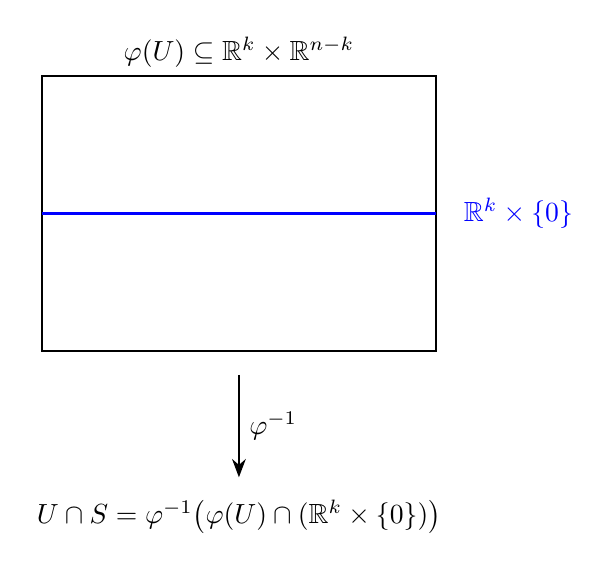
\begin{tikzpicture}[>=Stealth,scale=1]
\draw[thick] (0,0) rectangle (5,3.5);
\node at (2.5,3.8) {$\varphi(U)\subseteq\R^k\times\R^{n-k}$};
\draw[thick,blue] (0,1.75) -- (5,1.75);
\node[blue] at (6.05,1.75) {$\R^k\times\{0\}$};
\draw[->,thick] (2.5,-0.3) -- (2.5,-1.6) node[midway,right]{$\varphi^{-1}$};
\node at (2.5,-2.1) {$U\cap S=\varphi^{-1}\big(\varphi(U)\cap(\R^k\times\{0\})\big)$};
\end{tikzpicture}
\caption{Mapa plasterkowa: w mapie $\varphi$, przecięcie $U\cap S$ odpowiada dokładnie
przecięciu $\varphi(U)$ z podprzestrzenią $\R^k\times\{0\}$.}
\label{fig:plasterek}
\end{figure}

\begin{stwierdzenie}\label{stw:podrozm-struktura}
Jeśli $S\subseteq M$ jest podrozmaitością zanurzoną wymiaru $k$, to $S$ (z topologią
podprzestrzeni) jest rozmaitością topologiczną wymiaru $k$, posiadającą strukturę gładką,
względem której inkluzja $\iota\colon S\hookrightarrow M$ jest immersją; co więcej, $\iota$
jest zanurzeniem.
\end{stwierdzenie}
\begin{proof}
Wyposażamy $S$ w topologię podprzestrzeni. Ponieważ podprzestrzeń
przestrzeni Hausdorffa jest Hausdorffa, $S$ spełnia pierwszy warunek.
Jeśli $\mathcal B$ jest przeliczalną bazą $M$, to
$\{B\cap S:B\in\mathcal B\}$ jest przeliczalną bazą $S$:
dla otwartego $O\cap S$ i $p\in O\cap S$ znajdziemy
$B\in\mathcal B$ z $p\in B\subset O$, a wtedy
$p\in B\cap S\subset O\cap S$.

Ustalmy $p\in S$ i mapę plasterkową $(U,\varphi)$ przy $p$.
Ponieważ $U$ jest otwarte w $M$, zbiór $U_S=U\cap S$ jest otwarty
w $S$. Oznaczmy $W=\varphi(U)$, otwarty w $\R^n$.
Odwzorowanie $\varphi_S=\operatorname{pr}_1\circ\varphi|_{U_S}$
ma obraz $W_S=\{u\in\R^k:(u,0)\in W\}$, otwarty w $\R^k$ jako
przeciwobraz $W$ przez ciągłe zanurzenie $u\mapsto(u,0)$.
Odwrotność $u\mapsto\varphi^{-1}(u,0)$ jest ciągła; zatem
$\varphi_S:U_S\to W_S$ jest homeomorfizmem. To dowodzi lokalnej
euklidesowości $S$.

Niech teraz $(V,\psi)$ będzie drugą mapą plasterkową. Na
$\varphi_S(U\cap V\cap S)$ przejście ma wzór
\[
\psi_S\circ\varphi_S^{-1}(u)
=\operatorname{pr}_1\bigl((\psi\circ\varphi^{-1})(u,0)\bigr).
\]
Zanurzenie $u\mapsto(u,0)$, przejście $\psi\circ\varphi^{-1}$
i rzutowanie $\operatorname{pr}_1$ są gładkie, więc złożenie jest
gładkie. Zamieniając $\varphi$ i $\psi$, otrzymujemy gładką
odwrotność. Mapy $\varphi_S$ tworzą więc atlas gładki na $S$.

W mapach $\varphi_S$ i $\varphi$ inkluzja $\iota:S\to M$ ma postać
$u\mapsto(u,0)$, a jej różniczka wysyła $v$ na $(v,0)$ i jest
injektywna. Inkluzja jest więc immersją. Jako odwzorowanie
$S\to\iota(S)$ z \emph{topologią podprzestrzeni}, $\iota$ jest
homeomorfizmem już z wyboru topologii na $S$ (tożsamość na
zbiorze punktów). Zatem jest zanurzeniem.
\end{proof}



\begin{stwierdzenie}[Przestrzeń styczna do podrozmaitości]
\label{stw:styczna-podrozmaitosci}
\index{przestrzen styczna@Przestrzeń styczna!podrozmaitosci@podrozmaitości}
Niech $S\subseteq M$ będzie podrozmaitością zanurzoną wymiaru $k$
w rozmaitości $M$ wymiaru $n$, a $\iota\colon S\hookrightarrow M$
inkluzją. Dla $p\in S$ różniczka $d\iota_p$ utożsamia $T_pS$
z $k$-wymiarową podprzestrzenią $T_pM$. Jeśli mapa plasterkowa
przy $p$ ma współrzędne $(x^1,\ldots,x^k,y^1,\ldots,y^{n-k})$, to
\[
d\iota_p(T_pS)
=\operatorname{span}\left\{\left.\frac{\partial}{\partial x^i}\right|_p:
1\leq i\leq k\right\}
=\bigcap_{a=1}^{n-k}\ker(dy^a_p)\subseteq T_pM.
\]
Przy $k=0$ rozpiętość pustej rodziny oznacza $\{0\}$, a przy $k=n$
puste przecięcie oznacza $T_pM$.
Są to dokładnie prędkości $(\iota\circ\gamma)'(0)$ gładkich krzywych
$\gamma\colon(-\varepsilon,\varepsilon)\to S$ przechodzących przez $p$.
\end{stwierdzenie}
\begin{proof}
W mapie $\varphi_S$ na $S$ z dowodu
Stwierdzenia~\ref{stw:podrozm-struktura} inkluzja ma postać
$u\mapsto(u,0)$. Jej różniczka wysyła więc wektor o współrzędnych
$(a^1,\ldots,a^k)$ na $(a^1,\ldots,a^k,0,\ldots,0)$.
To daje pierwszy opis obrazu $d\iota_p$ i jego wymiar $k$.
Jeżeli $v\in T_pM$ ma współrzędne $(a^1,\ldots,a^k,b^1,\ldots,b^{n-k})$,
to $dy^a_p(v)=b^a$. Zatem wszystkie $dy^a_p(v)$ znikają dokładnie
wtedy, gdy $v$ należy do obrazu $d\iota_p$.

Każda krzywa w $S$ daje prędkość z tego obrazu na mocy reguły łańcucha.
Odwrotnie, dla dowolnego $(a^1,\ldots,a^k)$ krzywa
$\gamma(t)=\varphi_S^{-1}\bigl(\varphi_S(p)+t(a^1,\ldots,a^k)\bigr)$
jest określona dla dostatecznie małych $|t|$, leży w $S$ i jej prędkość
po inkluzji ma współrzędne $(a^1,\ldots,a^k,0,\ldots,0)$.
\end{proof}

\begin{przyklad}[Przestrzeń styczna do okręgu]
Niech $S^1=\{(x,y)\in\R^2:x^2+y^2=1\}$ i $p=(1,0)$.
Jest to jednowymiarowa podrozmaitość $\R^2$: dla
$f(x,y)=x^2+y^2$ różniczka $df_q(a,b)=2(q_1a+q_2b)$ jest niezerowa
w każdym $q=(q_1,q_2)\in S^1=f^{-1}(1)$, więc lokalna postać
submersji z Wniosku~\ref{wn:submersja-lokalnie} daje mapę plasterkową.
Jeśli $\eta(t)=(x(t),y(t))$ jest krzywą w $S^1$ przez $p$, to
różniczkowanie $x(t)^2+y(t)^2=1$ w $t=0$ daje $2x'(0)=0$.
Każda prędkość jest więc postaci $(0,b)$. Odwrotnie,
$\gamma_b(t)=(\cos bt,\sin bt)$ leży w $S^1$ i
$\gamma_b'(0)=(0,b)$. Stąd, przy $T_p\R^2\cong\R^2$,
\[
T_pS^1=\{(0,b):b\in\R\},\qquad
p+T_pS^1=\{(1,b):b\in\R\}.
\]
Pierwszy zbiór jest przestrzenią wektorów stycznych, a drugi ---
prostą styczną przechodzącą przez $p$ (rys.~\ref{fig:styczna-okrag}).
\end{przyklad}

\begin{figure}[ht]
\centering
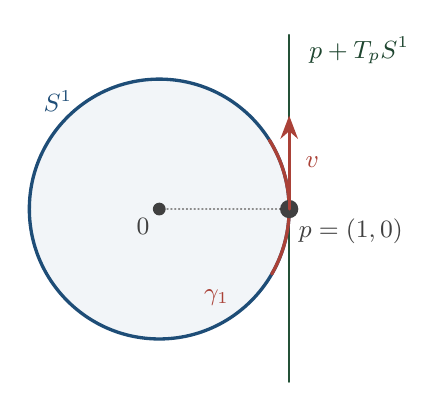
\begin{tikzpicture}[>=Stealth,scale=1.65,line cap=round,line join=round]
  \fill[manifoldblue!6] (0,0) circle (1);
  \draw[manifoldgreen!65!black,thick] (1,-1.33)--(1,1.34);
  \draw[black!45,densely dotted] (0,0)--(1,0);
  \draw[manifoldblue!85!black,very thick] (0,0) circle (1);
  \draw[manifoldred,very thick] plot[domain=-30:32,samples=30]
    ({cos(\x)},{sin(\x)});
  \fill[black!75] (0,0) circle (1.4pt) node[below left,font=\small] {$0$};
  \fill[black!75] (1,0) circle (2pt)
    node[below right,font=\small] {$p=(1,0)$};
  \draw[->,manifoldred,very thick] (1,0)--(1,.72)
    node[midway,right,font=\small,xshift=2pt] {$v$};
  \node[manifoldblue!85!black,font=\small] at (-.78,.83) {$S^1$};
  \node[manifoldred,font=\small] at (.44,-.68) {$\gamma_1$};
  \node[manifoldgreen!55!black,font=\small,anchor=west]
    at (1.08,1.22) {$p+T_pS^1$};
\end{tikzpicture}
\caption{Okrąg $S^1$ i jego prosta styczna w $p$. Czerwona krzywa
$\gamma_1$ biegnie po okręgu, a jej prędkość $v=\gamma_1'(0)=(0,1)$ wskazuje kierunek
styczny. Zielona prosta to przesunięcie przestrzeni wektorowej
$T_pS^1=\{(0,b):b\in\R\}$ do punktu $p$.}
\label{fig:styczna-okrag}
\end{figure}

\begin{przyklad}[Wiązka normalna jako wiązka ilorazowa]
Niech $S\subset M$ będzie podrozmaitością zanurzoną wymiaru $k$,
gdzie $\dim M=n$. Na mocy Stwierdzenia~\ref{stw:styczna-podrozmaitosci}
poprzez różniczkę inkluzji utożsamiamy
$T_pS$ z podprzestrzenią $T_pM$, a $TS$ traktujemy jako
podwiązkę wiązki ograniczonej $TM|_S$.

\emph{Wiązkę normalną} podrozmaitości $S$ definiujemy jako
wiązkę ilorazową $\nu S:=TM|_S/TS, \ \nu_pS:=T_pM/T_pS$.
Jej włókna są przestrzeniami wektorowymi wymiaru $n-k$.
Konstrukcja ta nie wymaga wyboru metryki ani dopełnienia
podprzestrzeni $T_pS$ w $T_pM$.

Pokażemy, że $\nu S$ jest wiązką wektorową rzędu $n-k$.
W mapie plasterkowej o współrzędnych $(x,y)$, gdzie
$x\in\R^k$ i $y\in\R^{n-k}$, podrozmaitość $S$ jest
opisana równaniem $y=0$. Wówczas
\[
T_pM=T_pS\oplus
\operatorname{span}\left\{
\left.\frac{\partial}{\partial y^1}\right|_p,
\ldots,
\left.\frac{\partial}{\partial y^{n-k}}\right|_p
\right\}.
\]
Każda klasa $[v]\in T_pM/T_pS$ ma zatem jednoznaczny
reprezentant w kierunkach $\partial/\partial y^a$,
co pozwala utożsamić lokalnie $\nu_pS$ z $\R^{n-k}$.

Sprawdźmy zmiany współrzędnych. Przejście między dwiema
mapami plasterkowymi ma postać $(x,y)\longmapsto(a(x,y),b(x,y))$,
przy czym $b(x,0)=0$. Różniczkując tę tożsamość
względem $x$, otrzymujemy $D_xb(x,0)=0$, więc
różniczka przejścia w punktach $S$ ma postać blokową
\[
\begin{pmatrix}
A&B\\
0&C
\end{pmatrix}.
\]
Cała macierz jest odwracalna, zatem kwadratowy blok
$C$ również jest odwracalny. Wektor o współrzędnych
$(u,v)\in\R^k\oplus\R^{n-k}$ przechodzi na $(u,v)\longmapsto(Au+Bv,Cv)$.
Ponieważ wektory styczne do $S$ odpowiadają
składowym $(u,0)$, klasa wektora w ilorazie
zmienia współrzędne według wzoru $[v]\longmapsto[Cv]$.
Zmiana ta zależy wyłącznie od składowej poprzecznej.

Macierze $C$ są gładkie i spełniają warunek kocyklu,
ponieważ różniczki przejść się składają, a iloczyn
macierzy blokowych zachowuje powyższą postać.
Twierdzenie o sklejaniu daje więc wiązkę wektorową
rzędu $n-k$ o włóknach $T_pM/T_pS$.

Otrzymujemy w ten sposób naturalny ciąg dokładny
wiązek wektorowych
\[
0\longrightarrow TS
\longrightarrow TM|_S
\longrightarrow \nu S
\longrightarrow 0.
\]
W szczególności konstrukcja wiązki normalnej jest
kanoniczna i nie wymaga żadnej dodatkowej struktury
geometrycznej na $M$.
\end{przyklad}


Poniższe twierdzenie i jego następstwa pokazują, w jaki sposób podrozmaitości powstają ,,w
praktyce'' — jako obrazy zanurzeń oraz jako przeciwobrazy wartości regularnych.

\begin{twierdzenie}[Twierdzenie o obrazie]\label{tw:obraz}
Jeśli $F\colon S\to M$ jest zanurzeniem ($\dim S=k\leq n=\dim M$), to $F(S)$ jest
podrozmaitością zanurzoną wymiaru $k$ w $M$, a $F\colon S\to F(S)$ (z topologią
podprzestrzeni) jest dyfeomorfizmem.
\end{twierdzenie}
\begin{proof}
Ustalmy $q=F(p_0)\in F(S)$. Ponieważ $F$ jest immersją w $p_0$, na mocy
Wniosku~\ref{wn:immersja-lokalnie} istnieją mapy $(U,\varphi)$ wokół $p_0$ w $S$ i
$(V,\psi)$ wokół $q$ w $M$, w których $F$ przyjmuje postać $u\mapsto(u,0)$.
Uzasadnijmy potrzebne dopasowanie dziedzin: wybieramy małe otwarte
kule $A\subset\R^k$, $B\subset\R^{n-k}$ o środku $0$, tak aby
$A\subset\varphi(U)$ i $A\times B\subset\psi(V)$.
Zastępujemy $U$ przez $\varphi^{-1}(A)$, a $V$ przez
$\psi^{-1}(A\times B)$. Wtedy rzeczywiście
$\psi(F(U))=A\times\{0\}=\psi(V)\cap(\R^k\times\{0\})$.
Zatem $(V,\psi)$ jest ,,prawie'' mapą
plasterkową dla $F(S)$, z tą różnicą, że warunek dotyczy $F(U)$, a nie od razu $F(S)\cap V$.

W tym miejscu wykorzystujemy założenie, że $F$ jest \emph{zanurzeniem}, nie tylko
różnowartościową immersją (por.\ Przykład~\ref{prz:osemka}): ponieważ $F\colon S\to F(S)$
jest homeomorfizmem na obraz, zbiór $F(U)$ jest otwarty w $F(S)$, tzn.\ $F(U)=F(S)\cap W$
dla pewnego otwartego $W\subseteq M$. Zastępując $V$ przez $V':=V\cap W$, otrzymujemy
$F(S)\cap V'=F(U)\cap V'$, a
\begin{align*}
\psi(F(S)\cap V')
 &=\psi(F(U)\cap V')\\
 &=\psi(F(U))\cap\psi(V')\\
 &=\big(\psi(V)\cap(\R^k\times\{0\})\big)\cap\psi(V')\\
 &=\psi(V')\cap(\R^k\times\{0\}).
\end{align*}
Zatem $(V',\psi|_{V'})$ jest mapą plasterkową rzędu $k$ dla $F(S)$ wokół $q$. Ponieważ
$q\in F(S)$ był dowolny, $F(S)$ jest podrozmaitością zanurzoną wymiaru $k$.

Wreszcie, $F\colon S\to F(S)$ jest bijekcją gładką (w mapach plasterkowych powyżej, $F$
przyjmuje postać identyczności), której odwrotność $F^{-1}\colon F(S)\to S$ jest gładka z
tego samego powodu. Zatem $F\colon S\to F(S)$ jest dyfeomorfizmem.
\end{proof}

\begin{definicja}
Niech $F\colon M\to N$ będzie gładkie, $q\in N$. Punkt $q$ jest \emph{wartością regularną}
$F$, jeśli dla każdego $p\in F^{-1}(q)$, $F$ jest submersją w $p$ (jeśli $F^{-1}(q)=
\emptyset$, $q$ jest — pusto — wartością regularną).
\end{definicja}

\begin{twierdzenie}[Twierdzenie o przeciwobrazie wartości regularnej]\label{tw:przeciwobraz}
Niech $F\colon M\to N$ będzie gładkie, $\dim M=m$, $\dim N=n$, i niech $q\in N$ będzie
wartością regularną $F$ z $F^{-1}(q)\neq\emptyset$. Wówczas $F^{-1}(q)$ jest
podrozmaitością zanurzoną wymiaru $m-n$ w $M$, a dla każdego $p\in F^{-1}(q)$,
$T_p\big(F^{-1}(q)\big)=\ker(dF_p)\subseteq T_pM$.
\end{twierdzenie}
\begin{proof}
Niech $p\in F^{-1}(q)$. Ponieważ $F$ jest submersją w $p$, na mocy
Wniosku~\ref{wn:submersja-lokalnie} istnieją mapy $(U,\varphi)$ wokół $p$ ($\varphi(p)=0$)
i $(V,\psi)$ wokół $q$ ($\psi(q)=0$), w których $F$ przyjmuje postać $\psi\circ F\circ
\varphi^{-1}(u^1,\dots,u^m)=(u^1,\dots,u^n)$. W tych mapach,
\[
\varphi(U\cap F^{-1}(q))=\{u\in\varphi(U):(u^1,\dots,u^n)=0\}=\varphi(U)\cap(\{0\}\times
\R^{m-n}).
\]
Po przenumerowaniu współrzędnych w $\R^m$ (zamiana miejscami pierwszych $n$ z pozostałymi
$m-n$), $(U,\varphi)$ staje się mapą plasterkową rzędu $m-n$ dla $F^{-1}(q)$ wokół $p$.
Ponieważ $p\in F^{-1}(q)$ był dowolny, $F^{-1}(q)$ jest podrozmaitością zanurzoną wymiaru
$m-n$.

W drugiej części niech $\iota\colon F^{-1}(q)\hookrightarrow M$
będzie inkluzją. Jest ona immersją na mocy
Stwierdzenia~\ref{stw:podrozm-struktura}. Ponieważ $F\circ\iota$ jest
odwzorowaniem stale równym $q$, jego różniczka znika: $dF_p\circ d\iota_p=0$ (reguła
łańcucha). Zatem $d\iota_p(T_pF^{-1}(q))\subseteq\ker(dF_p)$; utożsamiając (poprzez
injektywną różniczkę $d\iota_p$) $T_pF^{-1}(q)$ z jego obrazem w $T_pM$, mamy $T_pF^{-1}(q)
\subseteq\ker(dF_p)$. Z rachunku wymiarów: $\dim T_pF^{-1}(q)=m-n$ (z pierwszej części
dowodu), a $\dim\ker(dF_p)=m-\mathrm{rz}(dF_p)=m-n$ (bo $dF_p$ jest surjektywne na $T_qN$
wymiaru $n$, z definicji submersji). Zatem obie podprzestrzenie $T_pM$ mają ten sam,
skończony wymiar $m-n$, a jedna zawiera się w drugiej — więc są równe.
\end{proof}

\begin{wniosek}[Twierdzenie o poziomicy]
Jeśli $\dim M=n$, $f\colon M\to\R$ jest gładka, $c\in\R$ jest wartością regularną $f$ (tzn.\
$df_p\neq0$ dla każdego $p\in f^{-1}(c)$) i $f^{-1}(c)\neq\emptyset$, to $f^{-1}(c)$ jest
podrozmaitością zanurzoną wymiaru $n-1$ w $M$ (,,hiperpowierzchnią''), z $T_pf^{-1}(c)=
\ker(df_p)$.
\end{wniosek}
\begin{proof}
Szczególny przypadek Twierdzenia~\ref{tw:przeciwobraz} z $N=\R$: submersywność $f$ w
$p\in f^{-1}(c)$ to dokładnie warunek $df_p\neq0$.
\end{proof}

\begin{stwierdzenie}[Przestrzeń styczna i wektory normalne w $\R^m$]
\label{stw:styczna-normalne-euklidesowe}
Niech $S\subseteq\R^m$ będzie podrozmaitością zanurzoną wymiaru
$k<m$, a $p\in S$. Utożsamiajmy $T_pS$ z obrazem różniczki inkluzji
w $T_p\R^m\cong\R^m$. Załóżmy, że na otwartym otoczeniu $U$ punktu $p$
podrozmaitość jest opisana równaniami
\[
S\cap U=\{x\in U:f_1(x)=\cdots=f_{m-k}(x)=0\},
\]
gdzie $f_j\colon U\to\R$ są gładkie, a ich różniczki
$df_{1,q},\ldots,df_{m-k,q}$ są liniowo niezależne w każdym
$q\in S\cap U$. Wówczas
\[
T_pS=\bigcap_{j=1}^{m-k}\ker df_{j,p}
=\left(\operatorname{span}\{\nabla f_1(p),\ldots,
\nabla f_{m-k}(p)\}\right)^\perp\subseteq\R^m,
\]
gdzie $\nabla f_j(p)=
(\partial_1f_j(p),\ldots,\partial_mf_j(p))$ jest wektorem
współczynników różniczki względem standardowych współrzędnych.
Każda podrozmaitość zanurzona w $\R^m$ ma lokalnie taki opis:
funkcjami $f_j$ mogą być współrzędne poprzeczne mapy plasterkowej.
\end{stwierdzenie}
\begin{proof}
Odwzorowanie $F=(f_1,\ldots,f_{m-k})\colon U\to\R^{m-k}$
ma surjektywną różniczkę w każdym punkcie $S\cap U$,
bo jej składowe $df_{j,q}$ są liniowo niezależne. Zero jest więc
wartością regularną $F$. Z Twierdzenia~\ref{tw:przeciwobraz}
otrzymujemy $T_pS=\ker dF_p=\bigcap_j\ker df_{j,p}$.
W standardowym iloczynie skalarnym
$df_{j,p}(v)=\sum_{\ell=1}^m\partial_\ell f_j(p)v^\ell
=\langle\nabla f_j(p),v\rangle$.
Znikanie wszystkich tych iloczynów jest dokładnie prostopadłością
do rozpiętości wektorów $\nabla f_j(p)$.

W mapie plasterkowej $\varphi=(x^1,\ldots,x^k,y^1,\ldots,y^{m-k})$
można wybrać $f_j=y^j$: warunek $S\cap U=\{y=0\}$ jest częścią
definicji tej mapy, a różniczka $(y^1,\ldots,y^{m-k})$ jest
surjektywna, bo stanowi złożenie izomorfizmu $d\varphi_q$
z rzutowaniem na ostatnie $m-k$ współrzędnych.
\end{proof}

\begin{przyklad}
Niech $f\colon\R^{n+1}\to\R$, $f(x)=\|x\|^2$. Wtedy $df_x(v)=2\langle x,v\rangle$, niezerowe
dla $x\neq0$. Ponieważ $S^n=f^{-1}(1)$ i $0\notin f^{-1}(1)$, $1$ jest wartością regularną
— na mocy Wniosku powyżej, $S^n$ jest podrozmaitością zanurzoną wymiaru $n$ w $\R^{n+1}$
(zgodnie z tym, co wiedzieliśmy już z Przykładu~\ref{prz:sfera}; twierdzenie o poziomicy
daje jednak krótszy dowód gładkości struktury na $S^n$, choć nie podaje jawnych map).
\end{przyklad}

\begin{przyklad}[Grupa ortogonalna]
Niech $F\colon M_n(\R)\to\mathrm{Sym}(n)$, $F(A):=A^TA$, gdzie $\mathrm{Sym}(n)\cong
\R^{n(n+1)/2}$ oznacza przestrzeń macierzy symetrycznych. Dla $H\in T_AM_n(\R)\cong M_n(\R)$
stosujemy definicję różniczki przez krzywe do $\gamma(t)=A+tH$ w $M_n(\R)$:
\[
dF_A(H)=(F\circ\gamma)'(0)=\frac{d}{dt}\Big|_{t=0}(A+tH)^T(A+tH)=A^TH+H^TA.
\]
Dla $A\in\mathrm{O}(n):=F^{-1}(I)=\{A:A^TA=I\}$, $dF_A$ jest surjektywne na
$\mathrm{Sym}(n)$: dla symetrycznej $S$, kładąc $H:=\tfrac12AS$,
\[
dF_A(H)=A^T\big(\tfrac12AS\big)+\big(\tfrac12AS\big)^TA=\tfrac12(A^TA)S+\tfrac12S^TA^TA=
\tfrac12S+\tfrac12S=S
\]
(korzystając z $A^TA=I$, $S^T=S$). Zatem $I$ jest wartością regularną $F$, więc
$\mathrm{O}(n)=F^{-1}(I)$ jest podrozmaitością zanurzoną $M_n(\R)\cong\R^{n^2}$ wymiaru
$n^2-n(n+1)/2=n(n-1)/2$. Co więcej, $T_I\mathrm{O}(n)=\ker(dF_I)=\{H:H+H^T=0\}=:
\mathfrak{so}(n)$ — przestrzeń macierzy antysymetrycznych, wymiaru $n(n-1)/2$ (zgodnie z
powyższym rachunkiem wymiaru).
\end{przyklad}

\begin{uwaga}
Powyższy przykład jest pierwszym spotkaniem z fundamentalnym zjawiskiem: $\mathrm{O}(n)$
jest nie tylko rozmaitością, ale i grupą (względem mnożenia macierzy), w której mnożenie i
branie odwrotności są gładkie — tzw.\ \emph{grupą Liego} — a $T_I\mathrm{O}(n)=
\mathfrak{so}(n)$ jest jej \emph{algebrą Liego}.
\end{uwaga}

\begin{przyklad}[Torus jako regularna poziomica]
Niech $R>r>0$, $\rho=\sqrt{x^2+y^2}$ oraz
$\Omega=\{(x,y,z)\in\R^3:\rho>0\}$. Na tym otwartym zbiorze
$f(x,y,z)=(\rho-R)^2+z^2$ jest gładka. Poziom $f=r^2$
leży w $\Omega$, gdyż $|\rho-R|\leq r<R$ daje $\rho\geq R-r>0$.
Różniczka w punkcie $\Omega$ ma postać
\[
df=2(\rho-R)\left(\frac{x}{\rho}\,dx+
\frac{y}{\rho}\,dy\right)+2z\,dz.
\]
Jeżeli $df=0$, to $z=0$ oraz $\rho=R$: ponieważ $(x,y)\ne(0,0)$,
nie mogą jednocześnie znikać współczynniki przy $dx,dy$, chyba że
$\rho-R=0$. Lecz wtedy $f=0$, a więc taki punkt nie leży na
poziomie $r^2>0$. Zatem $r^2$ jest wartością regularną i torus
obrotowy $f^{-1}(r^2)$ jest gładką powierzchnią. Ponadto
$T_pT^2=\ker df_p$: wektor $(a,b,c)$ jest styczny wtedy i tylko
wtedy, gdy $(\rho-R)(xa+yb)/\rho+zc=0$.
\end{przyklad}

\par\smallskip
{\footnotesize\noindent\emph{Dalsza lektura:}
\href{https://www.ocw.mit.edu/courses/18-965-geometry-of-manifolds-fall-2004/34fad8f392208544e2b1e9794c33cbe7_lecture1.pdf}
{T.~S.~Mrowka, \emph{Geometry of Manifolds}, wykład~1},
definicje i przykłady rozmaitości;
\href{https://www.ocw.mit.edu/courses/18-965-geometry-of-manifolds-fall-2004/de18bf0029c583cacffb09810879bb54_lecture7.pdf}
{tenże, wykład~7}, wiązka styczna;
\href{https://pi.math.cornell.edu/~hatcher/VBKT/VB.pdf}
{A.~Hatcher, \emph{Vector Bundles and K-Theory}, \S\,1.1},
wiązki wektorowe.\par}

\clearpage

\chapter{Pola wektorowe, przepływy i pochodna Liego}
\label{ch:pola}
\index{pole wektorowe}

W Rozdziale~\ref{ch:rozmaitosci} zbudowaliśmy przestrzenie styczne i wiązkę $TM$.
Teraz wybieramy wektor \emph{w każdym} punkcie, w sposób gładki.
Otrzymujemy pole wektorowe: jednocześnie operator
różniczkowy, kierunek ruchu i infinitezymalny generator lokalnych dyfeomorfizmów.
Z tego jednego pojęcia wynikają nawias Liego, krzywe całkowe, przepływy oraz
pochodna Liego.

Rozdział rozwija rachunek pól oraz geometrię ich przepływów: najpierw
rozwiązujemy równanie krzywej całkowej, a następnie badamy ruch
punktów i sposób przenoszenia funkcji oraz pól wektorowych.
Do dalszej topologii różniczkowej przydadzą się zwłaszcza prostowanie
pola, pola zależne od czasu oraz rozszerzanie izotopii.
Przez $M$ rozumiemy rozmaitość gładką w sensie Definicji~\ref{def:rozmaitosc-gladka},
bez brzegu, chyba że wyraźnie zaznaczono inaczej.
Wszystkie pola i odwzorowania są klasy $C^\infty$.
Uwagi o brzegu i końcach przedziału czasu rozumiemy
według Definicji~\ref{def:rozmaitosc-z-brzegiem-1}
i opisu przestrzeni stycznej w
Stwierdzeniu~\ref{prop:styczna-brzeg-1}.
Tak samo interpretujemy gładkie rodziny na domkniętym przedziale czasu.



\section{Pola wektorowe i derywacje globalne}
\label{sec:derywacje}

W Sekcji~\ref{sec:przestrzen-styczna} utożsamiliśmy wektor $v\in T_pM$ z
\emph{derywacją w punkcie} $v\colon C^\infty(M)\to\R$:
po zastosowaniu do funkcji otrzymujemy liczbę. Pole wybiera taki
wektor w każdym punkcie, a jego działanie na funkcję zwraca nową
funkcję. Rozróżnienie tych dwóch typów derywacji będzie istotne.

\begin{definicja}
\emph{Pole wektorowe} $X$ na $M$ to gładka sekcja wiązki stycznej
$TM\to M$, czyli gładkie odwzorowanie $X\colon M\to TM$ spełniające
$X(p)\in T_pM$ dla każdego $p$. Przestrzeń pól oznaczamy $\X(M)=\Gamma(TM)$.
\end{definicja}

Wartość pola w ustalonym punkcie oznaczamy $X_p:=X(p)$.
Jest to jeden wektor styczny w $T_pM$; zapis $X_p(f)$ oznacza
działanie tego wektora jako derywacji w punkcie $p$ na funkcję $f$.
Na przykład wzór $X_{(u,v)}=(-v,u)$ na $\R^2$, po utożsamieniu
$T_{(u,v)}\R^2$ z $\R^2$, określa pole:
w każdym punkcie przypisuje wektor styczny zależny gładko od $(u,v)$.
Poza początkiem układu wektor jest styczny do okręgu o środku w zerze,
a w początku $X_{(0,0)}=0$.

W mapie $(U;x^1,\ldots,x^n)$ pole zapisuje się jednoznacznie jako
\begin{equation}\label{eq:lokalne-pole}
 X\big|_U=\sum_{i=1}^{n}X^i\frac{\partial}{\partial x^i},
 \qquad X^i\in C^\infty(U).
\end{equation}
Dokładniej, dla $p\in U$ jest to równość w $T_pM$:
$X_p=\sum_iX^i(p)\,\partial_{x^i}|_p$.
Lokalna trywializacja $TM$ z Rozdziału~\ref{ch:rozmaitosci}
pokazuje, że gładkość sekcji $X$ jest równoważna gładkości
wszystkich $X^i$ w każdej mapie. W drugą stronę gładkie współczynniki
na obszarach map określają jedno pole, jeżeli na przecięciach
opisują te same wektory styczne.

Geometrycznie $X_p$ wskazuje kierunek i prędkość w punkcie $p$.
Jeżeli $f\in C^\infty(M)$, czyli $f\colon M\to\R$,
opisuje na przykład temperaturę, to $X_p(f)$ jest chwilowym
tempem jej zmiany w kierunku wyznaczonym przez $X_p$.

Sprawdźmy tę interpretację na krzywej reprezentującej $X_p$.
W modelu z Sekcji~\ref{sec:przestrzen-styczna} każdy wektor
styczny jest reprezentowany przez klasę krzywych.
Wybierzmy mapę $(U,\varphi)$ wokół $p$, gdzie
$\varphi=(x^1,\ldots,x^n)$, i zapiszmy
$X_p=\sum_{i=1}^n X^i(p)\,\partial_{x^i}|_p$.
Na $\varphi(U)$ używamy standardowych współrzędnych
$u^1,\ldots,u^n$.
Oznaczmy $a=(X^1(p),\ldots,X^n(p))\in\R^n$ i rozważmy
krzywą $c(t)=\varphi(p)+ta$ w przestrzeni współrzędnych.
Ponieważ $\varphi(U)$ jest otwarty i $c(0)=\varphi(p)$,
istnieje $\varepsilon>0$ takie, że
$c((-\varepsilon,\varepsilon))\subset\varphi(U)$.
Możemy zatem zdefiniować
\[
\gamma\colon(-\varepsilon,\varepsilon)\to U,
\qquad
\gamma(t)=\varphi^{-1}\bigl(\varphi(p)+ta\bigr).
\]
Krzywa ta jest gładka i spełnia $\gamma(0)=p$ oraz
$(\varphi\circ\gamma)'(0)=a$, więc jej klasa $[\gamma]$
odpowiada wektorowi $X_p$ przy utożsamieniu
z rozdziału~1.

Pokażemy, że $X_p(f)$ jest pochodną funkcji $f$
wzdłuż skonstruowanej krzywej. Ponieważ
$\gamma=\varphi^{-1}\circ c$ i $\gamma(t)\in U$,
złożenie $f\circ\gamma$ jest dobrze określone oraz
$f\circ\gamma=(f\circ\varphi^{-1})\circ c$.
Stosując regułę łańcucha, otrzymujemy
\[
\begin{aligned}
\left.\frac{\dd}{\dd t}\right|_{t=0}f(\gamma(t))
&=D(f\circ\varphi^{-1})(\varphi(p))\cdot c'(0)\\
&=\sum_{i=1}^n X^i(p)
  \frac{\partial(f\circ\varphi^{-1})}{\partial u^i}
  (\varphi(p))
=X_p(f).
\end{aligned}
\]
Ostatnia równość wynika z definicji derywacji
współrzędnościowych. Rachunek obowiązuje dla każdej krzywej
o klasie $[\gamma]=X_p$: jej prędkość w mapie w chwili $t=0$
jest zawsze równa $a$. Niezależność tej klasy od wyboru mapy
ustaliliśmy w Sekcji~\ref{sec:przestrzen-styczna}.

Krzywa $\gamma$ reprezentuje zatem wektor w jednym
punkcie; jej dalszy przebieg nie wpływa na $X_p(f)$.
Nie musi być przy tym krzywą całkową pola $X$,
gdyż wymagamy jedynie zgodności jej wektora stycznego
z $X_p$ w chwili $t=0$.


\begin{definicja}
\emph{Derywacją} algebry $C^\infty(M)$ nazywamy $\R$-liniowe odwzorowanie
$D\colon C^\infty(M)\to C^\infty(M)$ spełniające regułę Leibniza
\[
 D(fg)=fD(g)+gD(f),\qquad f,g\in C^\infty(M).
\]
Zbiór takich derywacji oznaczamy $\operatorname{Der}_{\R}(C^\infty(M))$.
\end{definicja}

Warunek $\R$-liniowości oznacza liniowość względem stałych liczb.
Z reguły Leibniza wynika $D(1)=D(1\cdot1)=2D(1)$, więc $D(1)=0$
i $D(c)=0$ dla stałej $c$. Derywacja nie jest na ogół
$C^\infty(M)$-liniowa jako operator na funkcjach: jej działanie na
$hf$ zawiera dodatkowy składnik $fD(h)$.

Zacznijmy od pola $X$. Dla każdej funkcji $f\in C^\infty(M)$ określamy
\emph{funkcję} $D_X(f)$ przez
\[
 D_X(f)(p):=X_p(f),\qquad p\in M.
\]
W mapie $X_p=\sum_iX^i(p)\,\partial_i|_p$, więc
\[
 D_X(f)\big|_U=\sum_i X^i\partial_i f,
 \qquad D_X(f)(p)=\sum_iX^i(p)\,\partial_i f(p).
\]
W pierwszym wzorze $\partial_i f$ oznacza lokalną pochodną
$f\circ\varphi^{-1}$, przeniesioną z powrotem na $U$.
Suma gładkich funkcji jest gładka. Drugi wzór daje liczbę, bo
po ustaleniu $p$ współczynniki $X^i(p)$ są liczbami.
Punktowa reguła Leibniza dla $X_p$ daje
$D_X(fg)=fD_X(g)+gD_X(f)$ po sprawdzeniu równości w każdym punkcie.
Tak z pola otrzymujemy derywację globalną $D_X$.

W drugą stronę zacznijmy od \emph{dowolnej} derywacji globalnej $D$.
Dla ustalonego $p$ składamy ją z ewaluacją w $p$ i oznaczamy
\[
 v_p(f):=\bigl(D(f)\bigr)(p),\qquad
 C^\infty(M)\xrightarrow{\ D\ }C^\infty(M)
 \xrightarrow{\ \operatorname{ev}_p\ }\R.
\]
Funkcjonał $v_p$ jest $\R$-liniowy. Po ewaluacji globalnej
reguły Leibniza dostajemy \emph{punktową} regułę:
\[
 v_p(fg)=f(p)v_p(g)+g(p)v_p(f).
\]
Z definicji przestrzeni stycznej $v_p\in T_pM$; nie jest to już
operator o wartościach funkcyjnych. Lemat~\ref{lem:lokalnosc}
zapewnia, że $v_p(f)=D(f)(p)$ zależy tylko od kiełka $f$ w $p$.
Samo złożenie z ewaluacją daje na razie rodzinę wektorów;
jej gładkość trzeba jeszcze udowodnić.

\begin{twierdzenie}\label{thm:derywacje-pola}
Odwzorowanie
\[
 \X(M)\longrightarrow\operatorname{Der}_{\R}(C^\infty(M)),
 \qquad X\longmapsto D_X,\qquad D_X(f)(p)=X_p(f),
\]
jest izomorfizmem $C^\infty(M)$-modułów.
\end{twierdzenie}
\begin{proof}
Sprawdziliśmy wyżej, że $D_X$ jest derywacją, a dowolna
derywacja globalna $D$ wyznacza wektory $X_p(f):=D(f)(p)$.
Pozostaje pokazać, że $X\colon p\mapsto X_p$ jest gładką sekcją.

Ustalmy $p_0\in M$ i mapę $(U;x^1,\ldots,x^n)$ wokół $p_0$.
Wybierzmy otoczenie $V$ punktu $p_0$ o zwartym domknięciu zawartym w $U$
oraz funkcję odcinającą $\chi\in C^\infty(M)$, równą $1$ na
otoczeniu $\overline V$ i o nośniku zawartym w $U$.
Funkcja $\widetilde x^i$, zadana na $U$ przez $\chi x^i$ i równa
$0$ poza $U$, jest gładka na $M$. Na $V$ ma ten sam kiełek co $x^i$.
Z Twierdzenia~\ref{tw:baza-styczna} (po ewentualnym przesunięciu
początku współrzędnych) i lokalności derywacji punktowych
wynika, że dla $p\in V$
\[
 X_p=\sum_i a^i(p)\,\frac{\partial}{\partial x^i}\Big|_p,
 \qquad a^i(p)=X_p(\widetilde x^i)=D(\widetilde x^i)(p).
\]
Istotnie, działanie obu stron na $\widetilde x^j$ daje tę samą
liczbę $a^j(p)$, ponieważ
$\partial_{x^i}|_p(\widetilde x^j)=\delta_i^j$.
Każde $a^i=D(\widetilde x^i)|_V$ jest gładkie, gdyż $D$ przyjmuje
wartości w $C^\infty(M)$. Gładkość lokalnych współczynników
wokół każdego $p_0$ dowodzi gładkości $X$.

Dla każdego $f$ i $p$ mamy z konstrukcji
$D_X(f)(p)=X_p(f)=D(f)(p)$, zatem $D_X=D$.
Odwrotnie, jeśli zaczniemy od pola $X$, to ewaluacja $D_X$
w $p$ odzyskuje $X_p$ jako derywację punktową. Konstrukcje są więc
wzajemnie odwrotne. Dodawanie pól odpowiada dodawaniu derywacji,
a dla $h\in C^\infty(M)$ zachodzi
$D_{hX}(f)(p)=h(p)X_p(f)=(hD_X)(f)(p)$.
\end{proof}

Odtąd skracamy zapis $D_X(f)$ do $X(f)$; jest to funkcja na $M$,
podczas gdy $X_p(f)=X(f)(p)$ jest liczbą.

Na przykład na $\R$ operator $D(f)(x)=x^2f'(x)$ jest derywacją
globalną: $D(fg)(x)=x^2(f'(x)g(x)+f(x)g'(x))
=D(f)(x)g(x)+f(x)D(g)(x)$. Odpowiada mu pole
$X=x^2\partial_x$. W ustalonym punkcie $p$ jego wektor
$X_p=p^2\,\frac{\dd}{\dd x}\big|_p$ działa na funkcję przez
$X_p(f)=p^2f'(p)$; w szczególności $X_2(f)=4f'(2)$.
Współczynnik $x^2$ pola staje się liczbą $p^2$ po ustaleniu punktu.

\begin{uwaga}[Moduł pól i lokalne bazy]
Przestrzeń $\X(M)$ jest modułem nad pierścieniem funkcji:
$(hX)_p=h(p)X_p$. Po stronie derywacji mnożenie określa wzór
$(hD)(f)=hD(f)$; reguła Leibniza dla $hD$ wynika przez pomnożenie
obu stron reguły dla $D$ przez $h$.
Nie musi istnieć globalna baza modułu $\X(M)$ nad $C^\infty(M)$.
Na przykład $TS^2$ nie jest wiązką trywialną; nie da się wybrać
dwóch globalnych, wszędzie liniowo niezależnych pól na sferze.
Lokalne bazy $\partial_{x^1},\ldots,\partial_{x^n}$ zawsze istnieją.
Używamy tu klasycznego twierdzenia o nieistnieniu nigdzie
niezerowego pola na $S^2$; wynika ono również z późniejszego
Twierdzenia~\ref{thm:poincare-hopf-16} i $\chi(S^2)=2$.
\end{uwaga}

\begin{uwaga}[Przeniesienie pola przez mapę i zmiana współrzędnych]
Niech $(U,\varphi)$ będzie mapą rozmaitości $M$
o współrzędnych $x^1,\ldots,x^n$.
Ponieważ $\varphi\colon U\to\varphi(U)$ jest dyfeomorfizmem,
przenosi pole $X$ z $U$ na otwarty zbiór $\varphi(U)\subset\R^n$:
\begin{equation}\label{eq:pole-przeniesione-mapa}
\widehat X_\varphi(u)
:=(\dd\varphi)_{\varphi^{-1}(u)}X_{\varphi^{-1}(u)},
\qquad u\in\varphi(U).
\end{equation}
Piszemy $X_\varphi^i$ dla współczynników $X^i$
ze wzoru~\eqref{eq:lokalne-pole} w tej mapie;
indeks $\varphi$ odróżnia je od współczynników w innej mapie.
Jeśli $p=\varphi^{-1}(u)$ i
$X_p=\sum_iX_\varphi^i(p)\,\partial_{x^i}|_p$,
to współczynniki $\widehat X_\varphi(u)$ w standardowej bazie
$T_u\R^n$ wynoszą $X_\varphi^i(p)$.

W drugiej mapie $(V,\psi)$, o współrzędnych $y^1,\ldots,y^n$,
to samo pole ma na $U\cap V$ zapis
$X=\sum_jX_\psi^j\partial_{y^j}$.
Oznaczmy $G=\psi\circ\varphi^{-1}$.
Z reguły łańcucha dla $\psi=G\circ\varphi$ dostajemy
\[
\widehat X_\psi\bigl(G(u)\bigr)
=DG(u)\,\widehat X_\varphi(u),
\qquad u\in\varphi(U\cap V).
\]
Porównując $j$-te składowe, otrzymujemy regułę zmiany
współczynników pola:
\begin{equation}\label{eq:transformacja-wspolczynnikow-pola}
X_\psi^j(p)=\sum_i\frac{\partial y^j}{\partial x^i}(p)\,X_\varphi^i(p).
\end{equation}
Jest to ten sam rachunek co zmiana baz
z~\eqref{eq:transformacja-derywacji}.
Na przykład dla zmiany współrzędnej $y=2x$ na $\R$ pole
$X=a(x)\partial_x$ ma w nowej współrzędnej postać
$X=2a(y/2)\partial_y$.
\end{uwaga}

\begin{uwaga}[Od pola w przestrzeni otaczającej do współrzędnych]
Prześledźmy kolejność kroków, którą zastosujemy na okręgu i sferze.
Niech $M\subset\R^N$ będzie gładką podrozmaitością zanurzoną,
z inkluzją
$\iota\colon M\hookrightarrow\R^N$. Najpierw znamy pole $W$
na $\R^N$. Sprawdzamy, czy w punktach $p\in M$ jego wektor
$W_p\in T_p\R^N$ jest styczny do $M$, czyli należy do obrazu
$(\dd\iota)_p(T_pM)$. Dopiero wtedy możemy mówić o polu na samej
rozmaitości: ponieważ $(\dd\iota)_p$ jest injektywna
(Stwierdzenie~\ref{stw:styczna-podrozmaitosci}), istnieje
jedyny $X_p\in T_pM$ taki, że
\[
(\dd\iota)_pX_p=W_p.
\]
To są wektory w dwóch różnych przestrzeniach stycznych;
nie stosujemy $(\dd\varphi)_p$ bezpośrednio do $W_p$.
Gładkość $X$ wynika z gładkości $W$: w lokalnej parametryzacji
różniczka inkluzji ma rząd $\dim M$, więc współczynniki $X$
otrzymujemy lokalnie z gładkiego układu liniowego o nieosobliwym minorze.

Teraz wybieramy mapę $\varphi\colon U\to D\subset\R^n$ i piszemy
$u=\varphi(p)$. Korzystając ze wzoru~\eqref{eq:pole-przeniesione-mapa},
zapisujemy pole przeniesione na obszar współrzędnych $D$ jako
\[
\widehat X_\varphi(u)
=\sum_{i=1}^n a^i(u)\,
  \frac{\partial}{\partial u^i}\Big|_u,
\qquad a^i(u):=X_\varphi^i(\varphi^{-1}(u)).
\]
Liczby $a^i(u)=X_\varphi^i(p)$ są poszukiwanymi współczynnikami.
Wcześniejsza zmiana map porównywała dwa opisy \emph{tego samego}
pola $X$; tutaj przed użyciem mapy otrzymaliśmy $X$ z pola
otaczającego $W$. Jeśli $X$ jest już dane na $M$, zaczynamy
od wyboru mapy.

Dlaczego w rachunku pojawia się $\varphi^{-1}$? Aby porównać
nieznane współczynniki z danym wektorem $W_p$, wracamy z $D$
na $M$ przez $(\dd\varphi^{-1})_u$, a potem przechodzimy
do $\R^N$ przez $(\dd\iota)_p$. Równość
$(\dd\varphi^{-1})_u\widehat X_\varphi(u)=X_p$ wynika
z~$\varphi^{-1}\circ\varphi=\mathrm{id}_U$. Dla
$F=\iota\circ\varphi^{-1}\colon D\to\R^N$ reguła łańcucha daje
schemat w przestrzeniach stycznych:
\[
T_uD\ \xrightarrow{\ (\dd\varphi^{-1})_u\ }\ T_pM
\ \xrightarrow{\ (\dd\iota)_p\ }\ T_p\R^N,
\qquad
W_{F(u)}=(\dd F)_u\widehat X_\varphi(u)
=\sum_{i=1}^n a^i(u)\frac{\partial F}{\partial u^i}(u).
\]
Różniczka $\varphi^{-1}$ pokazuje więc, jak wektor zapisany
współrzędnymi wygląda na $M$; różniczka $F$ pokazuje ten sam
wektor w przestrzeni otaczającej. Ostatnie równanie pozwala
obliczyć $a^i(u)$ z podanego $W_p$ przez porównanie składowych.
\end{uwaga}

\begin{przyklad}[Pole obrotowe na okręgu]
Okrąg $S_r^1=\{(u,v)\in\R^2:u^2+v^2=r^2\}$, $r>0$,
jest jednowymiarową rozmaitością. Zanurzamy go w płaszczyźnie
przez inkluzję $\iota\colon S_r^1\hookrightarrow\R^2$,
$\iota(u,v)=(u,v)$; dla $r=1$ jest to zwykłe $S^1$.
Rozważmy na $\R^2$ pole
$W=-v\partial_u+u\partial_v$. Dla $p=(u,v)\in S_r^1$ mamy
$p\cdot W_p=-uv+vu=0$. Ponieważ przestrzeń styczna okręgu,
oglądana przez $(\dd\iota)_p$, jest prostopadła do $p$
(Stwierdzenie~\ref{stw:styczna-normalne-euklidesowe}),
$W_p$ jest styczny do okręgu. Dostajemy zatem jednoznaczne
pole $X$ na $S_r^1$ określone przez $(\dd\iota)_pX_p=W_p$.

Wybierzmy teraz otwarty przedział $I$ długości mniejszej niż $2\pi$.
Odwzorowanie $\gamma\colon I\to S_r^1$,
$\gamma(t)=(r\cos t,r\sin t)$, opisuje otwarty łuk
$U=\gamma(I)$ i jest odwrotnością lokalnej mapy kątowej
$\varphi\colon U\to I$. Po złożeniu z inkluzją otrzymujemy
parametryzację w płaszczyźnie
$F=\iota\circ\varphi^{-1}=\iota\circ\gamma\colon I\to\R^2$;
ma ona ten sam wzór $F(t)=(r\cos t,r\sin t)$.
Oznaczmy $p=\gamma(t)$. Na tym łuku zapis pola na rozmaitości
ma postać $X_p=a(t)\,\partial_t|_p$, gdzie
$a(t)=X_\varphi^1(\varphi^{-1}(t))$.
Chcemy znaleźć liczbę $a(t)$.
Zgodnie ze schematem przenosimy $X_p$ do $T_tI$ przez
$(\dd\varphi)_p$; otrzymujemy
$\widehat X_\varphi(t)=a(t)\,\partial_t|_t$.
Znamy jednak wektor $W_p$ w płaszczyźnie, więc porównamy oba
wektory po przeniesieniu z powrotem przez $(\dd F)_t$.
Reguła łańcucha daje
\[
\begin{aligned}
(\dd F)_t\!\left(\frac{\partial}{\partial t}\Big|_t\right)
&=\frac{\dd F}{\dd t}(t)
=(-r\sin t,r\cos t)\\
&=W_p.
\end{aligned}
\]
Ponieważ $(\dd F)_t=(\dd\iota)_p\circ(\dd\varphi^{-1})_t$,
różniczka odwrotności mapy przenosi $\partial_t|_t$ na wektor
bazy $\partial_t|_p$ na okręgu, a różniczka inkluzji pokazuje
go jako $(-r\sin t,r\cos t)$ w $T_p\R^2$.
Teraz
\[
W_p=(\dd F)_t\widehat X_\varphi(t)
=a(t)(-r\sin t,r\cos t).
\]
Pochodna $F'(t)$ jest niezerowa dla $r>0$, więc $a(t)=1$.
Równoważnie $X_p=\partial_t|_p$ i
$\widehat X_\varphi(t)=\partial_t|_t$. Wektor
$(-r\sin t,r\cos t)$ zapisujemy w bazie
$\partial_u|_p,\partial_v|_p$ przestrzeni $T_p\R^2$;
pojedynczy $\partial_u|_p$ na ogół nie jest styczny do okręgu.

Sprawdźmy teraz działanie pola na funkcje. Dla $g(u,v)=u$
otrzymujemy zmienną wzdłuż okręgu funkcję
$g\circ\gamma(t)=r\cos t$, a więc
$X(g|_{S_r^1})(\gamma(t))=\frac{\dd}{\dd t}(r\cos t)=-r\sin t$.
Natomiast dla $f(u,v)=u^2+v^2$ bierzemy
$h=f|_{S_r^1}$. Wzór współrzędnościowy daje
\[
X(h)\bigl(\gamma(t)\bigr)
=a(t)\frac{\dd}{\dd t}(h\circ\gamma)(t)
=\frac{\dd}{\dd t}\bigl(r^2\cos^2t+r^2\sin^2t\bigr)=0.
\]
Ta sama konstrukcja mapy działa lokalnie wokół każdego punktu okręgu.
Wynik $X(h)=0$ pokazuje, że pole nie zmienia wartości $f$ na
okręgu, zgodnie ze stycznością do poziomicy $f^{-1}(r^2)=S_r^1$.
Samo pole jest niezerowe, co widać z $F'(t)\ne0$.
\end{przyklad}

\begin{przyklad}[Pole na sferze]
Niech $S^2=\{(x,y,z)\in\R^3:x^2+y^2+z^2=1\}$.
Jak na okręgu, zaczynamy od pola w przestrzeni otaczającej:
$W=-y\partial_x+x\partial_y$ na $\R^3$, bez składowej
w kierunku $z$. Niech $\iota\colon S^2\hookrightarrow\R^3$
będzie inkluzją. W punkcie $p=(x,y,z)\in S^2$ wektor pola
otaczającego ma postać $W_p=(-y,x,0)$. Ponieważ
$p\cdot W_p=-xy+xy=0$, a obraz $(\dd\iota)_p(T_pS^2)$
jest płaszczyzną prostopadłą do $p$
(Stwierdzenie~\ref{stw:styczna-normalne-euklidesowe}),
$W_p$ jest styczny
do sfery. Określa zatem jednoznaczne gładkie pole $X$ na
$S^2$ przez $(\dd\iota)_pX_p=W_p$. Wzór na $W$ podaje
więc pole na całej sferze, zanim wybierzemy jakąkolwiek mapę.

Chcemy teraz odczytać współczynniki $X$ w jednej mapie.
Niech $U=\{(x,y,z)\in S^2:z>0\}$ będzie górną półsferą,
$D=\{(u,v)\in\R^2:u^2+v^2<1\}$, a
$\varphi\colon U\to D$ mapą $\varphi(x,y,z)=(x,y)=(u,v)$.
Współrzędne $x,y,z$ w $\R^3$ nie są trzema niezależnymi
współrzędnymi na $S^2$: wiąże je równanie $x^2+y^2+z^2=1$.
Na $U$ wystarczą dwie współrzędne $u,v$, gdyż
$z=\sqrt{1-u^2-v^2}>0$. W punkcie
$p=\varphi^{-1}(u,v)$ zapiszmy więc
$X_p=a(u,v)\,\partial_u|_p+b(u,v)\,\partial_v|_p$.
Po utożsamieniu $T_{(u,v)}D$ z $\R^2$ jego obraz ma postać
$\widehat X_\varphi(u,v)=(a(u,v),b(u,v))$.
Szukamy tych dwóch liczb.

Wiemy, jak wygląda $W_p$ w $\R^3$, więc znów wracamy ze
współrzędnych do przestrzeni otaczającej. Odwrotność mapy
razem z inkluzją daje parametryzację
\[
F=\iota\circ\varphi^{-1},\qquad
F(u,v)=(u,v,z(u,v)),\qquad
z(u,v)=\sqrt{1-u^2-v^2}.
\]
Różniczka $\varphi^{-1}$ przenosi wektory bazy z $D$
na wektory styczne do sfery, a $(\dd\iota)_p$ pokazuje je
w $\R^3$. Z reguły łańcucha
$(\dd F)_{(u,v)}=(\dd\iota)_p\circ(\dd\varphi^{-1})_{(u,v)}$.
Ponieważ $\partial_u z=-u/z$ i $\partial_v z=-v/z$,
\[
\dd F_{(u,v)}(a,b)
=a\left(1,0,-\frac{u}{z}\right)
 +b\left(0,1,-\frac{v}{z}\right)
=\left(a,b,-\frac{ua+vb}{z}\right).
\]
Teraz rozwiązujemy równanie ze schematu
$(\dd F)_{(u,v)}(a,b)=W_p=(-v,u,0)$.
Z pierwszych dwóch składowych dostajemy $a=-v$ i $b=u$;
trzecia też się zgadza, bo $u(-v)+vu=0$.
Stąd $X|_U=-v\,\partial_u+u\,\partial_v$.
Otrzymaliśmy ten sam wynik, który dałoby zastosowanie
$(\dd\varphi)_p$ do \emph{wektora stycznego $X_p$ na sferze}:
różniczka mapy bierze z jego obrazu w $\R^3$ pierwsze
dwie składowe. Nie stosujemy jej do pola $W$ zdefiniowanego
na całej $\R^3$.

Pole ma zera na biegunach; poza nimi wskazuje kierunek obrotu
wokół osi $z$. Na Rysunku~\ref{fig:pole-obrotowe-na-sferze}
wyróżniono punkt $p=(0,-\sqrt3/2,1/2)\in U$.
W naszej mapie $(u,v)=(0,-\sqrt3/2)$, więc
$X_p=(\sqrt3/2)\,\partial_u|_p$, a jego obraz w $\R^3$ to
$(\dd\iota)_pX_p=W_p=(\sqrt3/2,0,0)$.
\end{przyklad}

\begin{figure}[H]
\centering
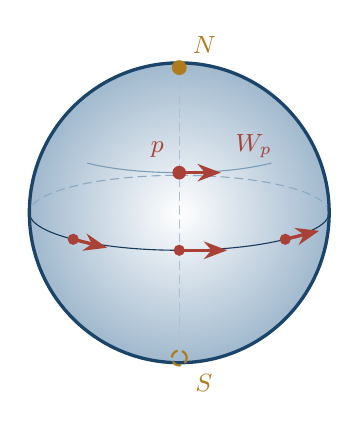
\begin{tikzpicture}[>=Stealth,scale=1.12,line cap=round,line join=round]
% Rzut ortogonalny P(x,y,z)=(x,(y+\sqrt{15}z)/4), ze skalą 1.7.
\shade[inner color=white,outer color=manifoldblue!43] (0,0) circle (1.7);
\coordinate (N) at (0,{1.7*sqrt(15)/4});
\coordinate (S) at (0,{-1.7*sqrt(15)/4});
\draw[manifoldblue!38,densely dashed,thin] (N)--(S);
% Tylna i przednia połowa równika.
\draw[manifoldblue!52,densely dashed,thin]
  (1.7,0) arc[start angle=0,end angle=180,x radius=1.7,y radius=.425];
\draw[manifoldblue!65!black,thin]
  (-1.7,0) arc[start angle=180,end angle=360,x radius=1.7,y radius=.425];
% Widoczny łuk równoleżnika z=1/2.
\draw[manifoldblue!60,thin]
  ({1.7*sqrt(3)/2*cos(225)},
   {1.7*sqrt(15)/8+1.7*sqrt(3)/8*sin(225)})
  arc[start angle=225,end angle=315,
      x radius={1.7*sqrt(3)/2},y radius={1.7*sqrt(3)/8}];
% Wektory są rzutami W_p=(-y,x,0), ze wspólną skalą długości.
\coordinate (pL) at ({1.7*cos(225)},{.425*sin(225)});
\coordinate (pE) at (0,-.425);
\coordinate (pR) at ({1.7*cos(315)},{.425*sin(315)});
\coordinate (p) at (0,{1.7*(sqrt(15)-sqrt(3))/8});
\fill[manifoldred] (pL) circle (1.8pt);
\fill[manifoldred] (pR) circle (1.8pt);
\fill[manifoldred] (pE) circle (1.8pt);
\draw[->,very thick,manifoldred] (pL)
  -- ++({.32*1.7/sqrt(2)},{-.32*.425/sqrt(2)});
\draw[->,very thick,manifoldred] (pR)
  -- ++({.32*1.7/sqrt(2)},{.32*.425/sqrt(2)});
\draw[->,very thick,manifoldred] (pE)
  -- ++(.544,0);
\draw[->,very thick,manifoldred] (p)
  -- ++({.32*1.7*sqrt(3)/2},0)
  node[above right=2pt,font=\small] {$W_p$};
\draw[manifoldblue!75!black,very thick] (0,0) circle (1.7);
\fill[manifoldred] (p) circle (2.2pt)
  node[above left=3pt,font=\small] {$p$};
\fill[manifoldgold!85!black] (N) circle (2.4pt)
  node[above right=2pt,font=\small] {$N$};
\draw[manifoldgold!85!black,densely dashed,thick] (S) circle (2.4pt)
  node[below right=3pt,font=\small] {$S$};
\end{tikzpicture}
\caption{Pole $X$ na sferze, oglądane przez $W_p=(-y,x,0)$ w $\R^3$.
Strzałki są styczne do
równoleżników i wskazują obrót wokół osi $z$. Bieguny $N$ i $S$
są zerami pola; przerywana obwódka oznacza zasłonięty biegun $S$.}
\label{fig:pole-obrotowe-na-sferze}
\end{figure}

\begin{uwaga}[Dwa sposoby obliczania pochodnej funkcji]
Gdy znamy współczynniki pola w mapie, obliczamy $X(f)(p)$
ze wzoru $X=\sum_iX^i\partial_{x^i}$, tak jak na okręgu.
Jeśli $M$ jest gładką podrozmaitością zanurzoną w $\R^N$,
możemy zamiast tego wybrać lokalne gładkie przedłużenie
$\widetilde f$ funkcji $f$ z $M$ do otoczenia $p$ w $\R^N$.
Takie przedłużenie istnieje: w lokalnym modelu, w którym $M$
jest zadana przez zerowe współrzędne normalne, nadajemy
$\widetilde f$ tę samą wartość niezależnie od tych współrzędnych.
Wtedy
$X_p(f)=W_p\cdot\nabla\widetilde f(p)$, gdzie
$(\dd\iota)_pX_p=W_p$: liczymy pochodną $\widetilde f$
wzdłuż krzywej w $M$ o wektorze stycznym $X_p$.
Wynik nie zależy od przedłużenia:
różnica dwóch przedłużeń znika na $M$, więc jej pochodna
wzdłuż każdej krzywej na $M$ jest równa zeru.
\end{uwaga}

\begin{uwaga}[Pole wzdłuż odwzorowania]
Dla gładkiego $F\colon M\to N$ i $X\in\X(M)$ wektory
$\dd F_p(X_p)$ leżą w przestrzeniach $T_{F(p)}N$.
Tworzą \emph{pole wzdłuż $F$}, czyli gładką sekcję wiązki cofniętej
\[
 F^*TN=\{(p,v):p\in M,\ v\in T_{F(p)}N\}\longrightarrow M,
 \qquad(p,v)\longmapsto p.
\]
Jeśli $x^i$ i $y^a$ są odpowiednio współrzędnymi na $M$ i $N$,
to współrzędne tego przekroju nad $p$ mają postać
$\sum_i X^i(p)\,\partial_i(y^a\circ F)(p)$.
Są gładkie, bo $X^i$ i $y^a\circ F$ są gładkie.
Pole wzdłuż $F$ ma za punkt bazowy $p\in M$, nawet gdy dwa różne
punkty $M$ mają ten sam obraz w $N$. Aby pochodziło od pola $Y$ na $N$,
musielibyśmy mieć
\[
 Y_{F(p)}=\dd F_p(X_p)\qquad\text{dla każdego }p\in M.
\]
Wektory po prawej stronie muszą zatem być równe przy wszystkich
przeciwobrazach jednego punktu.

Weźmy $M=N=\R$ oraz $X=\partial_t$ i oznaczmy współrzędną celu przez $y$.
Dla $F(t)=t^2$ reguła łańcucha daje
$\dd F_t(X_t)=2t\,\partial_y|_{t^2}$.
Jeśli $t>0$, punkty $t$ i $-t$ mają ten sam obraz $y=t^2$, więc
postulowane pole $Y$ musiałoby jednocześnie spełniać
\[
 Y_y=2t\,\partial_y|_y
 \qquad\text{oraz}\qquad
 Y_y=-2t\,\partial_y|_y.
\]
To niemożliwe, bo $t\ne0$. Nie otrzymujemy nawet jednoznacznego
przypisania wektora punktom obrazu $F$.

Dla $F(t)=t^3$ każdy $y\in\R$ ma dokładnie jeden przeciwobraz
$t=\sqrt[3]{y}$, więc nie ma już sprzeczności między przeciwobrazami.
Jedynym możliwym polem $Y$ byłoby jednak
\[
 \dd F_t(X_t)=3t^2\,\partial_y|_{t^3},
 \qquad
 Y_y=3|y|^{2/3}\,\partial_y|_y.
\]
Funkcja $a(y)=3|y|^{2/3}$ jest ciągła, lecz w zerze jej iloraz
różnicowy ma postać
\[
 \frac{a(h)-a(0)}{h}
 =3\,\operatorname{sgn}(h)|h|^{-1/3}\qquad(h\ne0),
\]
która nie ma skończonej granicy przy $h\to0$.
Nie istnieje więc gładkie pole $Y$ spełniające podany warunek.
Obie przeszkody dotyczą pary $(F,X)$: dla $F(t)=t^2$ i innego pola
$X=t\partial_t$ otrzymalibyśmy na przykład gładkie
$Y=2y\partial_y$ na $\R$.
Gdy $F$ jest dyfeomorfizmem, otrzymujemy natomiast pole
\[
 (F_*X)_q=\dd F_{F^{-1}(q)}X_{F^{-1}(q)}.
\]
Jest ono gładkie jako złożenie gładkich odwzorowań.
W szczególności $\varphi_*(X|_U)=\widehat X_\varphi$
ze wzoru~\eqref{eq:pole-przeniesione-mapa}.
Natomiast przyporządkowanie
$p\longmapsto(\dd\iota)_pX_p=W_p$ z obu przykładów
jest polem \emph{wzdłuż} inkluzji $\iota$;
wektory $W_p$ leżą w przestrzeniach stycznych do $\R^N$.
\end{uwaga}

\section{Nawias Liego: mierzenie nieprzemienności}
\label{sec:nawias}

Dwa pola są operatorami na funkcjach. Można je więc składać i wziąć
ich komutator.
\begin{definicja}
\emph{Nawiasem Liego} pól $X,Y\in\X(M)$ nazywamy pole $[X,Y]$ zadane przez
\begin{equation}\label{eq:nawias-def}
 [X,Y](f)=X(Y(f))-Y(X(f)),\qquad f\in C^\infty(M).
\end{equation}
\end{definicja}

Choć $X\circ Y$ jako operator jest na ogół drugiego rzędu, wyrazy z
pochodnymi drugimi znoszą się w różnicy.
\begin{fakt}\label{fakt:nawias-wlasnosci}
$[X,Y]$ jest polem wektorowym. Ponadto nawias jest dwuliniowy nad $\R$,
antysymetryczny i spełnia tożsamość Jacobiego
\[
 [X,[Y,Z]]+[Y,[Z,X]]+[Z,[X,Y]]=0.
\]
Jego reguła Leibniza względem funkcji ma postać
\begin{equation}\label{eq:nawias-leibniz}
 [X,fY]=f[X,Y]+X(f)Y,\qquad [fX,Y]=f[X,Y]-Y(f)X.
\end{equation}
\end{fakt}
\begin{proof}
Pokażmy najpierw, że komutator jest derywacją, choć samo
złożenie dwóch derywacji nią zazwyczaj nie jest.
Dla funkcji $f,g$ dwukrotnie stosujemy regułę Leibniza:
\begin{align*}
[X,Y](fg)
&=X\bigl(Y(f)g+fY(g)\bigr)
  -Y\bigl(X(f)g+fX(g)\bigr)\\
&=X(Yf)g+Y(f)X(g)+X(f)Y(g)+fX(Yg)\\
&\quad-Y(Xf)g-X(f)Y(g)-Y(f)X(g)-fY(Xg)\\
&=[X,Y](f)g+f[X,Y](g).
\end{align*}
Wyrazy mieszane znoszą się dokładnie parami. Komutator
jest liniowy nad $\R$ i spełnia regułę Leibniza,
więc z Twierdzenia~\ref{thm:derywacje-pola} odpowiada
gładkiemu polu wektorowemu. Z definicji natychmiast
$[X,Y]=-[Y,X]$; liniowość w obu argumentach wynika
z liniowości składania operatorów.

Sprawdźmy tożsamość Jacobiego, pokazując wszystkie
wyrazy. Jako operatory na funkcjach mamy
\begin{align*}
[X,[Y,Z]]&=XYZ-XZY-YZX+ZYX,\\
[Y,[Z,X]]&=YZX-YXZ-ZXY+XZY,\\
[Z,[X,Y]]&=ZXY-ZYX-XYZ+YXZ.
\end{align*}
Suma prawych stron jest zerowa: np.\ $XYZ$ znosi się
z $-XYZ$, a analogicznie pozostałe pięć możliwych
kolejności. Ponieważ równość operatorów zachodzi na
każdej funkcji, zachodzi równość pól wektorowych.

Na koniec stosujemy definicję do dowolnej funkcji $g$:
\begin{align*}
[X,fY](g)
 &=X\bigl(fY(g)\bigr)-fY\bigl(X(g)\bigr)
  =X(f)Y(g)+f[X,Y](g),\\
[fX,Y](g)
 &=fX\bigl(Y(g)\bigr)-Y\bigl(fX(g)\bigr)
  =f[X,Y](g)-Y(f)X(g).
\end{align*}
Funkcje rozróżniają pola, zatem są to dokładnie
równości~\eqref{eq:nawias-leibniz}.
\end{proof}

W mapie, jeśli $X=X^i\partial_i$ i $Y=Y^j\partial_j$, to
\begin{equation}\label{eq:nawias-wspolrzedne}
 [X,Y]=\sum_{j=1}^{n}\left(\sum_{i=1}^{n}
 X^i\frac{\partial Y^j}{\partial x^i}-
 Y^i\frac{\partial X^j}{\partial x^i}\right)\partial_j.
\end{equation}
Istotnie, współczynnik przy $\partial_j$ jest równy
$[X,Y](x^j)=X(Y^j)-Y(X^j)$; na funkcjach lokalnych możemy
działać dzięki lokalności derywacji. Tu i dalej $\partial_i$
skraca $\partial/\partial x^i$, a powtórzony indeks w zapisie
takim jak $X^i\partial_i$ oznacza sumowanie po tym indeksie.
Ważny wniosek: $[\partial_i,\partial_j]=0$ w układzie współrzędnych,
ale ogólne pola bazowe, np.\ ramy ruchome, nie muszą komutować.

Co sprawdza nawias? Wykonajmy krótki ruch najpierw wzdłuż $X$,
potem wzdłuż $Y$, i porównajmy go z ruchami w odwrotnej kolejności.
Końcowe punkty mogą się różnić. Jeśli oba ruchy trwają czas $t$,
to w mapie $x$ wokół $p$ różnica współrzędnych punktów końcowych
(kolejność $X,Y$ minus $Y,X$) ma postać
$t^2\,\dd x_p([X,Y]_p)+O(t^3)$. Dokładny rachunek z przepływami podamy
niżej przy Rysunku~\ref{fig:komutator-przeplywow}.
Jeśli $[X,Y]$ znika na otoczeniu, lokalne przepływy tych pól
komutują (Stwierdzenie~\ref{prop:inwarianty}).
Nawias wykrywa także, czy ruchy wzdłuż pól stycznych do rozkładu
wytwarzają kierunek poza nim; do tego wrócimy po przykładach.

\begin{przyklad}[Ścinanie płaszczyzny]\label{prz:scinanie}
Niech $X=\partial_x$ i $Y=x\partial_y$ na $\R^2$.
Wtedy $[X,Y]=\partial_y$. Najpierw przesunięcie w kierunku $x$
zmienia prędkość pionową $Y$; wykonanie ruchów w odwrotnej kolejności
daje inny wynik. Pole $Y$ ma zera na osi $x=0$ i nie jest polem
przesunięcia o stałej prędkości.
\end{przyklad}

\begin{przyklad}[Obrót i skalowanie]
Dla $R=-y\partial_x+x\partial_y$ i $E=x\partial_x+y\partial_y$
na $\R^2$ mamy $[R,E]=0$. Obrót i jednolite powiększenie
można wykonywać w dowolnej kolejności. Jeśli zaś
$X=\partial_x$, $Y=x\partial_y$, to wynik jest niezerowy
mimo że w punkcie $(0,0)$ mamy $Y=0$; nawias uwzględnia zmienność
pola w otoczeniu punktu.
\end{przyklad}



\begin{uwaga}[Rozkłady styczne i twierdzenie Frobeniusa]
Rozkład styczny wybiera w każdym punkcie $p$ podprzestrzeń
$\mathcal D_p\subset T_pM$ dopuszczalnych kierunków ruchu.
\emph{Gładkim rozkładem stałego rzędu} $0\leq k\leq n=\dim M$
nazywamy podwiązkę $\mathcal D\subset TM$ lokalnie rozpiętą
przez $k$ gładkich, punktowo liniowo niezależnych pól.
Pytamy, czy przez każdy punkt przechodzi lokalna
$k$-wymiarowa podrozmaitość $L$, dla której
$T_qL=\mathcal D_q$ w każdym $q\in L$.
Nazywamy ją \emph{podrozmaitością całkową} rozkładu.

Rozkład jest \emph{inwolutywny}, jeśli $[X,Y]$ jest jego sekcją
dla dowolnych lokalnych sekcji $X,Y$ rozkładu.
Wystarczy to sprawdzić na polach lokalnej bazy:
jeśli ich nawiasy należą do $\mathcal D$, to reguła
Leibniza~\eqref{eq:nawias-leibniz} daje tę samą własność
dla ich kombinacji o gładkich współczynnikach.
Twierdzenie Frobeniusa mówi, że jest to dokładnie warunek
istnienia przy każdym punkcie współrzędnych $(u^1,\ldots,u^n)$,
w których
\[
 \mathcal D=\operatorname{span}
 (\partial_{u^1},\ldots,\partial_{u^k}).
\]
Plasterki o stałych $u^{k+1},\ldots,u^n$ są wtedy lokalnymi
podrozmaitościami całkowymi, czyli fragmentami liści.

Na przykład na $\R^3$ pola
\[
 X=\partial_x+y\partial_z,\qquad
 Y=\partial_y+x\partial_z
\]
rozpinają rozkład $\mathcal D=\ker\dd(z-xy)$.
Rzeczywiście, $X(z-xy)=Y(z-xy)=0$, a pola są wszędzie
liniowo niezależne. Ich nawias znika:
$[X,Y]=\partial_z-\partial_z=0$.
Podrozmaitościami całkowymi są powierzchnie $z-xy=c$,
gdyż ich przestrzenie styczne są jądrami różniczki $\dd(z-xy)$.
Nie trzeba jednak wymagać, by wszystkie pola w rozkładzie
komutowały: $[X,xY]=Y\ne0$, lecz $Y$ nadal należy do
$\mathcal D$.

Inaczej jest dla rozkładu na $\R^3$
\[
 \mathcal D
 =\operatorname{span}\{\partial_x,\partial_y+x\partial_z\}.
\]
Nawias generatorów jest równy $\partial_z$, który nie należy do $\mathcal D$.
Składowe $x,y$ wymuszają bowiem zerowe współczynniki
ewentualnej kombinacji generatorów dającej $\partial_z$.
Nie ma zatem powierzchni, których przestrzenie styczne pokrywałyby się
z tym rozkładem. Dwa dozwolone ruchy wytwarzają tu
kierunek $\partial_z$ poza rozkładem.
Konieczność warunku jest widoczna już w mapie
plasterkowej: składowe normalne pól stycznych znikają na
podrozmaitości, więc ich pochodne w kierunkach stycznych również
tam znikają; wzór~\eqref{eq:nawias-wspolrzedne} pokazuje,
że nawias jest styczny. Dowód dostateczności podamy po twierdzeniu
o prostowaniu pola, w Stwierdzeniu~\ref{prop:frobenius-lokalny}.
Zastosujemy je później do lokalnego rozkładu metryki
w Twierdzeniu~\ref{thm:holonomia-lokalny-produkt}.
\end{uwaga}

\section{Krzywe całkowe i równania różniczkowe na rozmaitości}
\label{sec:krzywe}

\begin{definicja}
\emph{Krzywą całkową} pola $X$ nazywamy krzywą
$\gamma\colon I\to M$ na otwartym przedziale $I\subset\R$ spełniającą
\begin{equation}\label{eq:krzywa-calkowa}
 \gamma'(t)=X_{\gamma(t)}.
\end{equation}
Jeśli $0\in I$ i $\gamma(0)=p$, mówimy o krzywej wychodzącej z $p$.
Jest \emph{maksymalna}, gdy nie daje się przedłużyć jako rozwiązanie
na większy przedział.
\end{definicja}

W mapie, gdy $x^i(t)=x^i(\gamma(t))$ i
$X=\sum_i X^i\partial_{x^i}$,
warunek~\eqref{eq:krzywa-calkowa} staje się układem równań
różniczkowych zwyczajnych (ODE)
\[
 \frac{\dd x^i}{\dd t}=X^i(x^1(t),\ldots,x^n(t)),\qquad i=1,\ldots,n.
\]
Krzywa nie musi być prostą nawet wtedy, gdy wektory pola rysujemy
jako małe strzałki. W każdym swoim punkcie porusza się w kierunku
aktualnej strzałki; prędkość także jest przez nią określona.

\begin{twierdzenie}[Istnienie, jednoznaczność i zależność od danych]
\label{thm:ode}
Dla każdego $p\in M$ istnieje dokładnie jedna maksymalna krzywa
całkowa $\gamma_p\colon I_p\to M$ pola $X$, gdzie $I_p$ jest otwartym
przedziałem zawierającym $0$ i $\gamma_p(0)=p$.
Rozwiązania zależą gładko od czasu i punktu początkowego tam,
gdzie są określone.
\end{twierdzenie}
\begin{proof}
\emph{Krok 1: konstrukcja w mapie.}
Wybierzmy mapę $(U,\varphi)$ wokół $p$ o współrzędnych
$(u^1,\ldots,u^n)$ i połóżmy $D=\varphi(U)$, $u_0=\varphi(p)$.
Dla krzywej $\gamma$ pozostającej w $U$ oznaczmy
$u(t)=\varphi(\gamma(t))$. Pole przeniesione przez mapę
ze wzoru~\eqref{eq:pole-przeniesione-mapa}, po utożsamieniu
$T_vD$ z $\R^n$, jest gładkim odwzorowaniem $F\colon D\to\R^n$:
\[
 F(v)=(\dd\varphi)_{\varphi^{-1}(v)}X_{\varphi^{-1}(v)}
     =\bigl(X_\varphi^1(\varphi^{-1}(v)),\ldots,
             X_\varphi^n(\varphi^{-1}(v))\bigr).
\]
Reguła łańcucha przenosi równanie~\eqref{eq:krzywa-calkowa} na
\[
 u'(t)=(\dd\varphi)_{\gamma(t)}\gamma'(t)
      =(\dd\varphi)_{\gamma(t)}X_{\gamma(t)}=F(u(t)).
\]
Odwrotnie, jeśli $u'=F(u)$, to $\gamma=\varphi^{-1}\circ u$
spełnia $\gamma'=(\dd\varphi^{-1})_uF(u)=X_\gamma$.
Wybierzmy $r>0$ tak, aby domknięta kula
$\overline B_{2r}(u_0)$ leżała w $D$.
Na tej kuli istnieją stałe $A,L\geq 0$ spełniające
$\|F(u)\|\leq A$ oraz $\|\D F(u)\|\leq L$.
Twierdzenie o wartości średniej daje
$\|F(u)-F(v)\|\leq L\|u-v\|$ dla punktów tej kuli.
Wybierzmy $h>0$ tak, aby $hA<r$ i $hL<1$
(gdy $A=0$ lub $L=0$, odpowiedni warunek jest automatyczny).

Dla każdego warunku początkowego $a\in B_r(u_0)$ rozważmy
zupełną przestrzeń krzywych ciągłych
$z\colon[-h,h]\to\overline B_{2r}(u_0)$ z normą supremum.
Operator Picarda
\[
 (\mathcal T_a z)(t)=a+\int_0^t F(z(\tau))\,\dd\tau,
 \qquad t\in[-h,h],
\]
jest dobrze określony także dla $t<0$: wtedy całkujemy po
$[t,0]\subset[-h,h]$ z przeciwnym znakiem. Ponieważ $|t|\leq h$,
odwzorowuje tę przestrzeń w siebie:
\[
 \|\mathcal T_a z(t)-u_0\|
 \leq\|a-u_0\|+|t|A<r+hA<2r.
\]
Podobnie z oszacowania Lipschitza dla $F$ otrzymujemy
$\|\mathcal T_a z-\mathcal T_a w\|_\infty
 \leq hL\|z-w\|_\infty$.
Z twierdzenia Banacha o punkcie stałym otrzymujemy jedną
krzywą $z_a$ spełniającą równanie całkowe, a po zróżniczkowaniu
$z_a'(t)=F(z_a(t))$ dla $t\in(-h,h)$. Jest ona tam gładka
w czasie, bo $F$ jest gładkie. Lokalna jednoznaczność dotyczy
także dowolnego innego rozwiązania przez $a$: po zmniejszeniu
przedziału $[-\delta,\delta]\subset[-h,h]$ jego obraz leży w
$\overline B_{2r}(u_0)$, więc na tym przedziale oba rozwiązania
są punktami stałymi tego samego operatora kontrakcyjnego.

\emph{Krok 2: zależność od punktu początkowego.}
Z równań całkowych dla $z_a$ i $z_b$ oraz z oszacowania
kontrakcji otrzymujemy
\[
 \|z_a-z_b\|_\infty
 \leq \|a-b\|+hL\|z_a-z_b\|_\infty,
 \qquad
 \|z_a-z_b\|_\infty\leq\frac{\|a-b\|}{1-hL}.
\]
To dowodzi najpierw ciągłej zależności, jednak do gładkości
potrzeba więcej. Dla ustalonego $a$ rozwiążmy liniowe
równanie całkowe dla macierzy $J_a(t)$:
\[
 J_a(t)=I+\int_0^t\D F(z_a(\tau))J_a(\tau)\,\dd\tau.
\]
Operator po prawej, działający na ciągłe funkcje o wartościach
macierzowych, również ma stałą kontrakcji $hL<1$.
Istnieje więc jedyne $J_a$; spełnia ono równanie
wariacyjne $J_a'=\D F(z_a)J_a$, $J_a(0)=I$.

Sprawdźmy, że jest to rzeczywiście pochodna względem $a$.
Niech $v$ będzie na tyle małe, by $a+v\in B_r(u_0)$,
i połóżmy $\delta=z_{a+v}-z_a$.
Ponieważ $\D^2F$ jest ograniczona na $\overline B_{2r}(u_0)$,
rozwinięcie Taylora na odcinku między $z_a(\tau)$
a $z_{a+v}(\tau)$ daje, z pewną stałą $C$ niezależną
od $v$ i $\tau$,
\[
 \|F(z_a(\tau)+\delta(\tau))-F(z_a(\tau))
       -\D F(z_a(\tau))\delta(\tau)\|
 \leq C\|\delta\|_\infty^2.
\]
Odejmujemy równania całkowe dla $z_{a+v}$, $z_a$
i $J_av$. Dla $R=z_{a+v}-z_a-J_av$ dostajemy
\[
 \|R\|_\infty
 \leq hL\|R\|_\infty+hC\|\delta\|_\infty^2
 \leq hL\|R\|_\infty+
       \frac{hC}{(1-hL)^2}\|v\|^2.
\]
Zatem $\|R\|_\infty=O(\|v\|^2)$, co daje pochodną
$\D_a z_a=J_a$ jako odwzorowania do przestrzeni krzywych
ciągłych na $[-h,h]$. Dla jej ciągłości zauważmy,
że $\|J_a\|_\infty\leq(1-hL)^{-1}$ oraz
\[
 \|J_a-J_b\|_\infty
 \leq\frac{h}{(1-hL)^2}
 \|\D F(z_a)-\D F(z_b)\|_\infty.
\]
Prawa strona dąży do zera dla $b\to a$, dzięki ciągłości
$a\mapsto z_a$ i jednostajnej ciągłości $\D F$ na zwartej kuli.
Dalsze pochodne otrzymujemy w ten sam sposób, rozdzielając
konstrukcję kandydata od sprawdzenia, że jest pochodną.
Na przykład kandydat na drugą pochodną
$H_a(t)[v,w]$ spełnia
\[
 H_a(t)[v,w]=\int_0^t\bigl(
 \D F(z_a)H_a[v,w]
 +\D^2F(z_a)[J_av,J_aw]\bigr)(\tau)\,\dd\tau.
\]
Najpierw rozwiązujemy to liniowe równanie całkowe dla $H_a$
w przestrzeni ciągłych krzywych na $[-h,h]$ o wartościach
w przestrzeni odwzorowań dwuliniowych.
Część zawierająca $H_a$ ma stałą kontrakcji $hL$.
Następnie odejmujemy równania dla $J_{a+v}$, $J_a$ oraz
kandydata $H_a[v,\cdot]$. Wzór Taylora dla $\D F$ i
już dowiedziona różniczkowalność $z_a$ dają dla reszty
oszacowanie $\|R\|_\infty\leq hL\|R\|_\infty+o(\|v\|)$.
Stąd $\|R\|_\infty=o(\|v\|)$ i $H_a=\D_aJ_a$.
Ciągłość $a\mapsto H_a$ wynika z tego samego oszacowania
kontrakcyjnego: $z_a$ i $J_a$ zależą ciągle od $a$,
więc współczynnik $\D F(z_a)$ i wymuszenie
$\D^2F(z_a)[J_a,J_a]$ są ciągłe w normie supremum.

Ogólnie, dla $k\ge3$, połóżmy $Z_0=z_a$ i załóżmy,
że pochodne $Z_j=\D_a^j z_a$ dla $1\le j<k$
już istnieją i są ciągłe w $a$ jako krzywe na $[-h,h]$.
W $k$-krotnym różniczkowaniu złożenia $F(z_a)$ jedyny wyraz
zawierający nieznane $Z_k$ to $\D F(z_a)Z_k$.
Pozostałe wyrazy tworzą znane ciągłe wymuszenie $G_k$,
złożone z pochodnych $\D^mF(z_a)$ i $Z_j$ dla $j<k$.
Kandydata $Z_k$ określa więc równanie
\[
 Z_k(a,t)=\int_0^t\bigl(\D F(z_a(\tau))Z_k(a,\tau)
                         +G_k(a,\tau)\bigr)\,\dd\tau
 \qquad(k\ge3).
\]
Na ciągłych krzywych o wartościach w przestrzeni odwzorowań
$k$-liniowych jego prawa strona jest kontrakcją ze stałą $hL$.
Porównujemy teraz równania dla $Z_{k-1}(a+v)$, $Z_{k-1}(a)$
i kandydata $Z_k(a)[v,\cdot]$.
$G_{k-1}$ zawiera tylko $Z_j$ dla $j\le k-2$; ich pochodne
są już znane, więc $G_{k-1}$ ma jednostajne w czasie
rozwinięcie pierwszego rzędu względem $v$.
Ponadto $\D F(z_{a+v})-\D F(z_a)=O(\|v\|)$, a z ciągłości
$Z_{k-1}$ wynika $Z_{k-1}(a+v)-Z_{k-1}(a)=o(1)$.
Iloczyn tych dwóch różnic jest $o(\|v\|)$; pozostałe
reszty mają ten sam rząd dzięki jednostajnej ciągłości
pochodnych $F$ na zwartej kuli. Stąd dla różnicy $R$
$\|R\|_\infty\leq hL\|R\|_\infty+o(\|v\|)$.
To dowodzi $Z_k=\D_aZ_{k-1}$. Odwzorowania
$a\mapsto\D F(z_a)$ i $a\mapsto G_k(a,\cdot)$ są ciągłe
w normie supremum; równanie kontrakcyjne lokalnie ogranicza
$\|Z_k(a)\|_\infty$. Porównanie jego wersji dla $a$ i $b$
daje zatem ciągłość $Z_k$. Indukcja dowodzi gładkości
$a\mapsto z_a$.

Aby sprawdzić pochodne mieszane, zdefiniujmy gładkie odwzorowania
$V_0(v)=v$ i $V_{m+1}(v)=\D V_m(v)F(v)$ na $D$.
Z równania $z_a'=F(z_a)$ i reguły łańcucha wynika indukcyjnie
$\partial_t^m z_a(t)=V_m(z_a(t))$. Prawa strona zależy
gładko od $a$ jako krzywa ciągła, a wszystkie jej pochodne
po $a$ są ciągłe wspólnie w $(t,a)$. Otrzymujemy gładkość
$(t,a)\mapsto z_a(t)$ na $(-h,h)\times B_r(u_0)$.

\emph{Krok 3: przedział maksymalny.}
Dwie krzywe całkowe wychodzące z $p$ są równe w pobliżu zera
na mocy powyższej jednoznaczności. Zbiór czasów, w których
się zgadzają, jest domknięty w części wspólnej ich
przedziałów przez ciągłość obu krzywych. Jest też otwarty:
w punkcie, w którym się zgadzają, stosujemy lokalną
jednoznaczność ponownie. Ponieważ część wspólna jest przedziałem,
krzywe pokrywają się wszędzie, gdzie obie są określone.
Można więc skleić wszystkie rozwiązania przez $p$ na sumie
ich przedziałów. Suma ta jest otwartym przedziałem $I_p$
zawierającym zero; sklejenie daje rozwiązanie, którego żadne
dalsze przedłużenie nie istnieje. Jednoznaczność w mapach
zapewnia, że konstrukcja nie zależy od wyboru współrzędnych.
Dotąd wykazaliśmy gładką zależność na wspólnym krótkim przedziale
wokół zera. Dla dowolnego $t_0\in I_{p_0}$ zwarty odcinek krzywej
od czasu $0$ do $t_0$ dzielimy na skończenie wiele fragmentów,
na których działają lokalne konstrukcje z kroków 1--2.
Ich gładkie złożenie daje wspólną dziedzinę i gładką zależność
w otoczeniu $(t_0,p_0)$. Szczegóły tego sklejania,
w tym otwartość dziedziny wszystkich par $(t,p)$,
podajemy w dowodzie Twierdzenia~\ref{thm:przeplyw}.
\end{proof}

Jeśli $X_p=0$, to jedyną krzywą wychodzącą z $p$ jest krzywa stała.
Jeśli dwie krzywe całkowe spotkają się, to po odpowiednim przesunięciu
parametru czasu pokrywają się tam, gdzie obie są określone.
Mogą więc tworzyć orbitę okresową, lecz nie mogą przecinać się
transwersalnie jako trajektorie tego samego pola.

\begin{przyklad}[Obrót]
Na $\R^2$ niech $X=-y\partial_x+x\partial_y$. Układ
$x'=-y$, $y'=x$ daje
\begin{equation}\label{eq:obrot}
 \gamma_{(a,b)}(t)=(a\cos t-b\sin t,\ a\sin t+b\cos t).
\end{equation}
Dla $(a,b)\ne(0,0)$ trajektorią jest okrąg o promieniu
$\sqrt{a^2+b^2}$, przebiegany przeciwnie do ruchu wskazówek zegara.
Początek układu jest punktem stałym.
\end{przyklad}

\begin{figure}[!htbp]
\centering
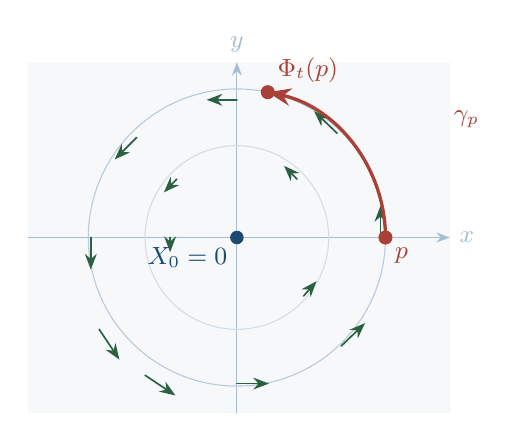
\begin{tikzpicture}[>=Stealth,scale=1.06,line cap=round]
\fill[manifoldblue!4] (-2.5,-2.1) rectangle (2.55,2.1);
\draw[->,manifoldblue!40] (-2.5,0)--(2.55,0) node[right,font=\small] {$x$};
\draw[->,manifoldblue!40] (0,-2.1)--(0,2.1) node[above,font=\small] {$y$};
\draw[manifoldblue!20] (0,0) circle (1.1);
\draw[manifoldblue!32] (0,0) circle (1.78);
\foreach \xx/\yy in {-1.65/-1.1,-1.1/-1.65,0/-1.75,1.25/-1.3,1.72/0,
 1.2/1.25,0/1.65,-1.2/1.2,-1.75/0,-.8/0,.72/.7,-.72/.7,.8/-.7}{
 \draw[->,manifoldgreen!78!black,semithick]
 (\xx,\yy)--++({-.22*\yy},{.22*\xx});}
\draw[manifoldred,very thick,->] (1.78,0)
 arc[start angle=0,end angle=78,radius=1.78];
\fill[manifoldred] (1.78,0) circle (2.4pt)
 node[below right,font=\small] {$p$};
\fill[manifoldred] ({1.78*cos(78)},{1.78*sin(78)}) circle (2.4pt)
 node[above right,font=\small] {$\Phi_t(p)$};
\fill[manifoldblue!80!black] (0,0) circle (2.3pt)
 node[below left,font=\small] {$X_0=0$};
\node[font=\small,manifoldred] at (2.75,1.42) {$\gamma_p$};
\end{tikzpicture}
\caption{Pole obrotowe $X=(-y,x)$: zielone strzałki przedstawiają wartości
pola pomniejszone wspólnym czynnikiem $0.22$,
a czerwona krzywa jest jego krzywą całkową. Strzałka pola
w każdym punkcie jest styczna do trajektorii.}
\label{fig:obrot-krzywa}
\end{figure}

\begin{przyklad}[Zmiana prędkości bez zmiany orbit]
Jeżeli $Y=fX$, gdzie $f>0$, to $X$ i $Y$ wyznaczają te same
\emph{zorientowane ślady} krzywych całkowych, choć czas ich
przebiegania jest inny. Gdy $f$ zmienia znak, orientacja ruchu może się
zmienić; gdy znika, pojawiają się punkty stałe. Dlatego sam obraz
krzywych nie wyznacza pola ani jego przepływu.
Dokładniej, jeśli $\gamma:I\to M$ jest krzywą $X$ z $\gamma(0)=p$,
to funkcja
\[
 s(\tau)=\int_0^\tau\frac{du}{f(\gamma(u))}
\]
ma dodatnią pochodną i jest dyfeomorfizmem $I$ na pewien
przedział $J$. Dla odwrotności $\tau=\tau(s)$ krzywa
$\eta(s)=\gamma(\tau(s))$ spełnia
$\eta'=f(\eta)X_\eta=Y_\eta$. Ta sama konstrukcja z $X=Y/f$
pokazuje równość orbit maksymalnych. Dokładniej, gdyby $\eta$
dała się przedłużyć przez skończony koniec $J$, równanie
$\tau'(s)=f(\eta(s))$ dawałoby tam skończoną wartość $\tau$
i dodatnią pochodną. Odwrotna zmiana czasu przedłużyłaby wtedy
$\gamma$ przez koniec $I$, wbrew jej maksymalności.
Przedziały czasu mogą
jednak być różne: zupełne $X=\partial_x$ po pomnożeniu przez
$f(x)=1+x^2$ daje niezupełne pole z krzywą $\tan s$ przez zero.
\end{przyklad}

\section{Przepływ lokalny, maksymalny i zupełny}
\label{sec:przeplyw}

Krzywe całkowe dla wszystkich punktów początkowych łączą się
w jedno odwzorowanie. W czasie $t$ przesuwamy punkt o tyle, ile
pozwala równanie~\eqref{eq:krzywa-calkowa}.

\begin{definicja}
Niech $\gamma_p\colon I_p\to M$ będzie maksymalną krzywą całkową.
\emph{Dziedziną maksymalnego przepływu} jest zbiór
$\mathcal D_X=\{(t,p)\in\R\times M:t\in I_p\}$, a
\emph{przepływem} pola $X$ odwzorowanie
\[
 \Phi\colon\mathcal D_X\to M,\qquad \Phi(t,p)=\Phi_t(p):=\gamma_p(t).
\]
Pole jest \emph{zupełne}, jeśli $\mathcal D_X=\R\times M$.
\end{definicja}

\begin{twierdzenie}[Podstawowe własności przepływu]
\label{thm:przeplyw}
Zbiór $\mathcal D_X$ jest otwarty, a $\Phi$ jest gładki. Zachodzi
\[
 \Phi_0=\id_M,\qquad
 \Phi_{t+s}(p)=\Phi_t(\Phi_s(p))
\]
dokładnie dla $s\in I_p$ i $t\in I_{\Phi_s(p)}$; przy tym
$I_{\Phi_s(p)}=I_p-s$. Dla $M_t:=\{p\in M:t\in I_p\}$
odwzorowania $\Phi_t\colon M_t\to M_{-t}$ i $\Phi_{-t}$ są wzajemnie
odwrotnymi dyfeomorfizmami między otwartymi zbiorami. Ponadto
\begin{equation}\label{eq:przeplyw-generuje}
 \left.\frac{\dd}{\dd t}\right|_{t=0}\Phi_t(p)=X_p,
 \qquad (\dd\Phi_t)_pX_p=X_{\Phi_t(p)}.
\end{equation}
Jeśli $X$ jest zupełne, $(\Phi_t)_{t\in\R}$ jest jednoparametrową
grupą dyfeomorfizmów.
\end{twierdzenie}
\begin{proof}
\emph{Otwartość i gładkość.}
Kroki 1--2 poprzedniego dowodu dają dla każdego $q\in M$
otoczenie $W_q$ i liczbę $\varepsilon_q>0$, wspólną
dla punktów początkowych z $W_q$, na której lokalne
rozwiązanie istnieje i jest gładkie względem czasu
i punktu początkowego.
Ustalmy $(t_0,p_0)\in\mathcal D_X$; rozważmy najpierw
$t_0>0$. Krzywa $\gamma_{p_0}$ jest określona
na pewnym otwartym przedziale obejmującym $[0,t_0]$.
Jej obraz $K=\gamma_{p_0}([0,t_0])$ jest zwarty.
Z pokrycia $K$ przez otwarte zbiory $W_q$ wybierzmy
skończone podpokrycie $W_{q_1},\ldots,W_{q_m}$.
Liczba $\varepsilon=\min_i\varepsilon_{q_i}$ jest dodatnia:
z każdego punktu $K$ można rozpocząć lokalne
rozwiązanie przez czas co najmniej $\varepsilon$.
Podzielmy odcinek czasu na
\[
 0=\tau_0<\tau_1<\cdots<\tau_N=t_0
\]
o długościach $\tau_{j+1}-\tau_j<\varepsilon/2$.
Każdy krok wzdłuż $\gamma_{p_0}$ jest wtedy
fragmentem lokalnego rozwiązania z jednego $W_{q_i}$.

Dla $j=0$ lokalny przepływ o czas
$\tau_1-\tau_0$ jest określony i gładki na pewnym
otoczeniu $p_0$. Jego obraz punktu $p_0$ to
$\gamma_{p_0}(\tau_1)$. Ciągłość pozwala zmniejszyć
otoczenie tak, by obrazy pobliskich punktów
należały do dziedziny następnego kroku. Powtarzając
ten argument skończenie wiele razy, otrzymujemy
otoczenie $V$ punktu $p_0$, na którym
$p\mapsto\Phi_{t_0}(p)$ jest gładkim złożeniem
lokalnych rozwiązań. W otoczeniu punktu
$\Phi_{t_0}(p_0)$ można prowadzić rozwiązanie
jeszcze przez wspólny krótki czas $u$.
Po ewentualnym zmniejszeniu $V$ wzór
\[
 \Phi_{t_0+u}(p)
 =\Phi_u\bigl(\Phi_{t_0}(p)\bigr)
\]
wynika z jednoznaczności i definiuje gładkie odwzorowanie
dla $(u,p)$ bliskich $(0,p_0)$. To samo rozumowanie
działa dla $t_0<0$, idąc po krzywej wstecz; przy
$t_0=0$ wystarcza konstrukcja lokalna.
W konsekwencji każde $(t_0,p_0)\in\mathcal D_X$
ma otoczenie zawarte w $\mathcal D_X$, na którym
$\Phi$ jest gładkie. Dowodzi to zarazem otwartości
dziedziny i gładkości przepływu.

\emph{Przesunięcie czasu i prawo grupowe.}
Niech $s\in I_p$ i $q=\Phi_s(p)$. Krzywa
$u\mapsto\gamma_p(s+u)$, określona na $I_p-s$, jest
rozwiązaniem wychodzącym z $q$, więc z jednoznaczności
$I_p-s\subset I_q$. W szczególności $-s\in I_q$.
Krzywa $v\mapsto\gamma_q(v-s)$, określona na $s+I_q$,
jest rozwiązaniem przez $p$ w chwili $v=0$.
Maksymalność $\gamma_p$ daje $s+I_q\subset I_p$.
Oba zawierania dowodzą $I_q=I_p-s$ i
\[
 \Phi_u(q)=\gamma_q(u)=\gamma_p(s+u)=\Phi_{s+u}(p)
 \quad\text{dla każdego }u\in I_q.
\]
Gdy $s\in I_p$, warunki $u\in I_q$ i $s+u\in I_p$
są więc równoważne. Zatem równość składania
obowiązuje dokładnie przy warunkach podanych w tezie.
Szczególny przypadek $s=0$ daje
$\Phi_0(p)=p$.

\emph{Odwrotności i generator.}
Ponieważ $\mathcal D_X$ jest otwarty, każdy $M_t$ jest otwarty.
Jeśli $q=\Phi_t(p)$, to $-t\in I_q$ i prawo składania
daje $\Phi_{-t}(q)=p$. Ten sam argument z zamienionymi
$t$ i $-t$ pokazuje, że $\Phi_t(M_t)=M_{-t}$;
gładkość obu odwzorowań daje dyfeomorfizm.
Pierwszy wzór w~\eqref{eq:przeplyw-generuje} jest równaniem
krzywej całkowej w chwili zero. Dla drugiego różniczkujemy
względem $s$ w zerze równość
$\Phi_t(\Phi_s(p))=\Phi_s(\Phi_t(p))$.
Po lewej stronie reguła łańcucha daje
$(\dd\Phi_t)_pX_p$, po prawej $X_{\Phi_t(p)}$.

Jeżeli $X$ jest zupełne, $M_t=M$ dla każdego $t$.
Wtedy wszystkie $\Phi_t$ są dyfeomorfizmami całej
rozmaitości i
$\Phi_{t+s}=\Phi_t\circ\Phi_s$, $\Phi_0=\id_M$,
$\Phi_t^{-1}=\Phi_{-t}$. Składanie dyfeomorfizmów
jest łączne, a wzór na parametry daje wprost
$\Phi_r\circ(\Phi_s\circ\Phi_t)=\Phi_{r+s+t}
=(\Phi_r\circ\Phi_s)\circ\Phi_t$.
Odwzorowanie $t\mapsto\Phi_t$ jest więc homomorfizmem
$(\R,+)\to\operatorname{Diff}(M)$, a
$(t,p)\mapsto\Phi_t(p)$ jest gładkim działaniem tej
grupy na $M$. Dla pola niezupełnego te same wzory
mają sens tylko w opisanych wyżej otwartych dziedzinach.
\end{proof}

\begin{stwierdzenie}[Grupa przepływu wyznacza swoje pole]
Jeśli gładkie odwzorowanie $H\colon\R\times M\to M$ spełnia
$H_0=\id_M$ i $H_{t+s}=H_t\circ H_s$, to
\[
 X_p:=\left.\frac{\dd}{\dd t}\right|_{t=0}H_t(p)
\]
jest gładkim zupełnym polem wektorowym, a $H_t=\Phi_t^X$
dla wszystkich $t\in\R$.
\end{stwierdzenie}
\begin{proof}
Prawo grupowe daje $H_t\circ H_{-t}=H_{-t}\circ H_t
=H_0=\id_M$. Zatem każdy $H_t$ jest dyfeomorfizmem
o gładkiej odwrotności $H_{-t}$.
Gładkość $H$ zapewnia gładkość przyporządkowania $p\mapsto X_p$.
Z prawa grupowego $H_{t+h}(p)=H_h(H_t(p))$ otrzymujemy,
różniczkując względem $h$ w zerze,
\[
 \frac{\dd}{\dd t}H_t(p)=X_{H_t(p)},\qquad H_0(p)=p.
\]
Zatem $t\mapsto H_t(p)$ jest krzywą całkową $X$ dla każdego
$t\in\R$. Jednoznaczność maksymalnej krzywej daje
$H_t(p)=\Phi_t^X(p)$; istnienie $H_t(p)$ dla wszystkich
czasów dowodzi zupełności pola.
\end{proof}

\begin{figure}[!htbp]
\centering
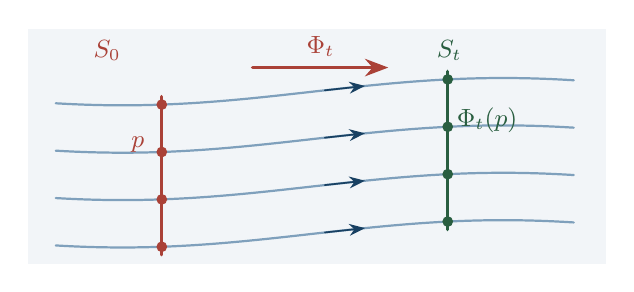
\begin{tikzpicture}[>=Stealth,scale=1.02,line cap=round]
\fill[manifoldblue!6] (-3.55,-1.42) rectangle (3.65,1.5);
\foreach \c in {-1.05,-.46,.13,.72}{
 \draw[manifoldblue!58,thick]
 plot[domain=-3.2:3.25,samples=55]
 ({\x},{\c+.17*sin(38*\x)});
 \draw[->,manifoldblue!70!black,semithick]
 ({.15},{\c+.17*sin(38*.15)})
 --({.65},{\c+.17*sin(38*.65)});
}
\draw[manifoldred,very thick] (-1.88,{-1.15+.17*sin(38*-1.88)})--(-1.88,{.82+.17*sin(38*-1.88)});
\draw[manifoldgreen!75!black,very thick] (1.68,{-1.15+.17*sin(38*1.68)})--(1.68,{.82+.17*sin(38*1.68)});
\foreach \c in {-1.05,-.46,.13,.72}{
 \fill[manifoldred] (-1.88,{\c+.17*sin(38*-1.88)}) circle (1.9pt);
 \fill[manifoldgreen!75!black] (1.68,{\c+.17*sin(38*1.68)}) circle (1.9pt);
}
\node[font=\small,manifoldred] at (-2.56,1.23) {$S_0$};
\node[font=\small,manifoldgreen!75!black] at (1.7,1.23) {$S_t$};
\node[font=\small,manifoldred] at (-2.18,.06) {$p$};
\node[font=\small,manifoldgreen!75!black] at (2.17,.36) {$\Phi_t(p)$};
\draw[->,very thick,manifoldred] (-.75,1.02)--(.94,1.02)
 node[midway,above,font=\small] {$\Phi_t$};
\end{tikzpicture}
\caption{Przepływ przesuwa punkty wzdłuż krzywych całkowych.
Czerwony przekrój poprzeczny $S_0$ przechodzi w zielony $S_t$;
oba przekroje mają dokładnie te same wartości stałej
$y-A\sin(\kappa x)$, gdzie $A=0.17$ i $\kappa=38\pi/180$.
Są to trajektorie pola $X=(1,A\kappa\cos(\kappa x))$.
Jego przepływ to
$\Phi_s(x,y)=(x+s,y+A[\sin(\kappa(x+s))-\sin(\kappa x)])$;
na rysunku $t=1.68-(-1.88)=3.56$.}
\label{fig:rura-przeplywu}
\end{figure}

\begin{przyklad}[Trzy zupełne przepływy]
Na $\R^n$ pole stałe $X=v$ ma $\Phi_t(x)=x+tv$.
Pole Eulera $E=\sum_i x^i\partial_i$ ma $\Phi_t(x)=e^t x$.
Pole obrotowe z~\eqref{eq:obrot} ma
$\Phi_t(a,b)=(a\cos t-b\sin t,a\sin t+b\cos t)$.
Wszystkie rozwiązania są określone dla całego $t\in\R$.
\end{przyklad}

\begin{przyklad}[Ucieczka w skończonym czasie]\label{prz:niezupelne}
Dla $X=x^2\partial_x$ na $\R$ krzywa przez $x_0$ spełnia
\[
 \Phi_t(x_0)=\frac{x_0}{1-tx_0},\qquad x_0\ne0.
\]
Jeśli $x_0>0$, jej dziedzina to $(-\infty,1/x_0)$; jeśli $x_0<0$,
to $(1/x_0,\infty)$. Dla $x_0=0$ krzywa jest stała i istnieje
dla wszystkich czasów. Pole jest gładkie na całej prostej,
ale nie jest zupełne: nieograniczony wzrost rozwiązania powoduje
ucieczkę do nieskończoności w skończonym czasie.
\end{przyklad}

\begin{twierdzenie}[Kryterium przedłużenia i dwa warunki zupełności]
\label{thm:zupelnosc}
Jeśli maksymalna krzywa całkowa ma skończony prawy koniec $b$, to
opuszcza w pobliżu $b$ każdy zwarty podzbiór $M$.
W konsekwencji każde pole na rozmaitości zwartej jest zupełne.
Każde pole o zwartym nośniku na dowolnej rozmaitości także jest zupełne.
\end{twierdzenie}
\begin{proof}
\emph{Kryterium przedłużenia.}
Niech $I_p=(a,b)$ i $b<\infty$. Załóżmy przeciwnie,
że istnieją zbiór zwarty $K\subset M$ i ciąg
$t_j\nearrow b$ taki, że $\gamma_p(t_j)\in K$.
Po wybraniu podciągu mamy $\gamma_p(t_j)\to q\in K$.
Lokalne twierdzenie o istnieniu w $q$ daje otoczenie
$W\ni q$ i $\varepsilon>0$ takie, że z każdego punktu
$W$ można prowadzić rozwiązanie przez wszystkie czasy
$u\in(-\varepsilon,\varepsilon)$.
Dla dużego $j$ zachodzi $\gamma_p(t_j)\in W$
oraz $b-t_j<\varepsilon/2$.
Krzywa
\[
 u\longmapsto\Phi_u(\gamma_p(t_j)),\qquad
 -\varepsilon<u<\varepsilon,
\]
pokrywa się z $u\mapsto\gamma_p(t_j+u)$ w ich wspólnej
dziedzinie, bo obie zaczynają w $\gamma_p(t_j)$.
Możemy więc skleić je w krzywą określoną także dla
$t> b$, sprzecznie z maksymalnością $I_p$.
Przy skończonym lewym końcu stosujemy ten sam argument
do pola $-X$ i czasu odwróconego.

\emph{Zupełność na zbiorach zwartych.}
Jeśli $M$ jest zwarta, każda trajektoria przez cały czas
leży w jednym zwartym zbiorze $M$. Kryterium wyklucza
oba skończone końce $I_p$, zatem $I_p=\R$.
Teraz niech $K=\supp X$ będzie zwarty.
Jeśli $p\notin K$, to $X_p=0$, więc krzywa
stała w $p$ jest, z jednoznaczności, całą krzywą
maksymalną. Jeśli $p\in K$, krzywa nie może wejść
do $M\setminus K$: od chwili wejścia byłaby stała,
a jednoznaczność, zastosowana także wstecz w czasie,
zmusiłaby ją do bycia stałą już w chwili zero.
W obu przypadkach obraz $\gamma_p$ leży w zwartym
zbiorze $K\cup\{p\}$; kryterium znów daje $I_p=\R$.
\end{proof}

\begin{uwaga}[Nie mylić zupełności z brakiem zer]
Zupełne pole może mieć zera (obrót na płaszczyźnie), a pole bez zer
może być niezupełne, np.\ $X=(1+x^2)\partial_x$ na $\R$.
Dla rozmaitości z brzegiem pole musi dodatkowo być styczne do brzegu,
aby dać dwustronny przepływ zachowujący tę rozmaitość.
Istotnie, dyfeomorfizmy zachowują brzeg, więc różniczkowanie
krzywej $t\mapsto\Phi_t(p)$ dla $p\in\partial M$ daje
$X_p\in T_p\partial M$. Odwrotnie, dla pola stycznego do brzegu
rozwiązujemy równanie również na $\partial M$; jednoznaczność
w lokalnym przedłużeniu pola zapewnia, że jego krzywe przez
brzeg pozostają na brzegu. Krzywe z wnętrza nie mogą go
przekroczyć, bo przy pierwszym spotkaniu jednoznaczność wstecz
wymuszałaby wcześniejszy pobyt na brzegu.
Pole skierowane do wnętrza na brzegu daje zwykle przepływ tylko
dla małych dodatnich czasów, co wykorzystamy do budowania kołnierza.
Na przykład na $M=[0,\infty)$ pole $X=\partial_r$ jest gładkim
przekrojem pełnej wiązki stycznej, także w $0$.
Krzywa całkowa zaczynająca się w $0$ musiałaby mieć postać
$r(t)=t$, więc dla $t<0$ opuszczałaby $M$.
Nie ma tu sprzeczności ze Stwierdzeniem~\ref{prop:styczna-brzeg-1}:
$T_0M\cong\R$, ale $T_0\partial M=\{0\}$ i $X_0\notin T_0\partial M$.
Styczność do brzegu zapewnia lokalny przepływ dwustronny;
jego istnienie dla wszystkich czasów wymaga ponadto zupełności.
\end{uwaga}

\section{Geometria przepływu: prostowanie, niezmienniki, komutowanie}
\label{sec:prostowanie}

\begin{definicja}[Orbita i nasycenie przez przepływ]
\index{orbita i nasycenie przez przeplyw@Orbita i nasycenie przez przepływ}
\emph{Orbitą} punktu $p$ pod przepływem pola $X$ jest
$\mathcal O_X(p)=\{\Phi_t(p):t\in I_p\}$.
Dla $A\subseteq M$ jego \emph{nasycenie przez przepływ}
to suma orbit punktów z $A$:
\[
 \operatorname{Sat}_X(A)=\bigcup_{p\in A}\mathcal O_X(p).
\]
Zbiór $A$ jest \emph{nasycony przez $X$}, gdy
$\operatorname{Sat}_X(A)=A$, czyli gdy
$p\in A$ i $t\in I_p$ pociągają za sobą
$\Phi_t(p)\in A$.
\end{definicja}

To jest nasycenie względem relacji ,,leżeć na tej samej
orbicie'' w sensie Definicji~\ref{def:nasycenie}.
Istotnie, gdy $q=\Phi_s(p)$, to
$I_q=I_p-s$ i $\mathcal O_X(q)=\mathcal O_X(p)$
na mocy Twierdzenia~\ref{thm:przeplyw}; orbity rozcinają
więc $M$ na rozłączne klasy. Na przykład dla
$X=\partial_x$ na $\R^2$ nasyceniem
$\{0\}\times(0,1)$ jest cały pas $\R\times(0,1)$.

\begin{twierdzenie}[Twierdzenie o prostowaniu pola]\label{thm:flowbox}
Jeśli $X_p\ne0$, to istnieją współrzędne $(t,z^2,\ldots,z^n)$
w otoczeniu $p$, w których $X=\partial_t$. W tych współrzędnych
lokalny przepływ ma postać
\[
 (t,z^2,\ldots,z^n)\longmapsto(t+s,z^2,\ldots,z^n).
\]
\end{twierdzenie}
\begin{proof}
Wybieramy małą $(n-1)$-wymiarową podrozmaitość $S$
przechodzącą przez $p$ i poprzeczną do $X_p$, oraz parametryzację
$\sigma\colon V\subset\R^{n-1}\to S$ z $\sigma(0)=p$.
Można ją zbudować bez dodatkowego twierdzenia: wybieramy mapę
z $p=0$ i po liniowej zmianie współrzędnych z pierwszą składową
$X_p$ niezerową; bierzemy $S=\{x^1=0\}$ w tej mapie.
Odwzorowanie $F(t,z)=\Phi_t(\sigma(z))$ ma w $(0,0)$
różniczkę, której pierwszą kolumną jest $X_p$, a pozostałe kolumny
rozpinają $T_pS$. Jest więc izomorfizmem. Z twierdzenia o funkcji
odwrotnej $F$ jest lokalnym dyfeomorfizmem. Zmniejszamy jego
dziedzinę do produktu $(-\varepsilon,\varepsilon)\times V_0$.
Ponieważ $\partial_tF(t,z)=X_{F(t,z)}$, we współrzędnych $F^{-1}$
pole ma postać $\partial_t$. Prawo grupowe daje
$\Phi_s(F(t,z))=F(t+s,z)$, dopóki $t$ i $t+s$ leżą
w tym przedziale. To wyjaśnia lokalny zakres wzoru z tezy.
\end{proof}

\begin{uwaga}
Pola nie można wyprostować w zerze $X_p=0$: dyfeomorfizm przenosi
wektor zerowy na wektor zerowy, natomiast $\partial_t$ nigdzie
nie znika. W zerze lokalne trajektorie i zachowanie przepływu
bada się innymi metodami niż prostowanie pola.
\end{uwaga}

\begin{stwierdzenie}[Lokalne twierdzenie Frobeniusa]
\label{prop:frobenius-lokalny}
Gładki rozkład inwolutywny $\mathcal D$ stałego rzędu $k$
ma lokalnie współrzędne, w których jest rozpięty przez pierwsze
$k$ pól współrzędnych.
\end{stwierdzenie}
\begin{proof}
Przeprowadzimy indukcję po $k$, jednocześnie dla wszystkich
wymiarów rozmaitości. Dla $k=0$ teza jest natychmiastowa.
Dla $k\ge1$ wybieramy lokalną bazę $X_1,\ldots,X_k$ rozkładu
i prostujemy niezerowe $X_1$. Mamy więc współrzędne $(t,z)$
w produkcie wokół $(0,0)$, z $X_1=\partial_t$.
Od każdego $X_j$, $j\ge2$, odejmujemy jego składową w kierunku
$\partial_t$. Otrzymane pola $Y_2,\ldots,Y_k$ nie mają tej
składowej, a wraz z $\partial_t$ nadal stanowią bazę $\mathcal D$.
Jeśli $k=1$, dowód jest już zakończony.

Niech $B(t,z)$ będzie macierzą o $k-1$ kolumnach złożonych
ze składowych $Y_2,\ldots,Y_k$ w kierunkach $z$.
Inwolutywność daje $[\partial_t,Y_j]\in\mathcal D$;
ponieważ ten nawias nie ma składowej czasowej, jest kombinacją
samych $Y_2,\ldots,Y_k$. Zatem
\[
 \partial_tB(t,z)=B(t,z)A(t,z)
\]
dla pewnej gładkiej macierzy kwadratowej $A$.
Gładkość współczynników wynika z rozwiązania układu za pomocą
niezerowego minora macierzy $B$, po zmniejszeniu otoczenia.
Rozwiązujemy macierzowe równanie
\[
 \partial_tQ(t,z)=-A(t,z)Q(t,z),\qquad Q(0,z)=I.
\]
Istnienie i gładka zależność od $z$ wynikają z
Twierdzenia~\ref{thm:ode}: dołączamy zmienne z równaniami
$t'=1$, $z'=0$. Po zmniejszeniu produktu $Q$ jest odwracalna,
bo $Q(0,0)=I$. Reguła iloczynu daje
\[
 \partial_t(BQ)=BAQ-BAQ=0,\qquad B(t,z)Q(t,z)=B(0,z).
\]
Kolumny $BQ$ wyznaczają więc nową bazę pól pionowych
niezależnych od $t$, rozpinającą te same kierunki co kolumny $B$.
Na przekroju $t=0$ tworzą rozkład rzędu $k-1$.
Jest on inwolutywny: nawiasy tych pól nie mają składowej
czasowej, należą do $\mathcal D$ i nie zależą od $t$;
reguła Leibniza dla nawiasu rozszerza to na dowolne sekcje.
Z założenia indukcyjnego istnieje zmiana współrzędnych $z$
prostująca ten rozkład. Stosujemy ją niezależnie od $t$.
Ponieważ baza pionowa nie zależy od czasu, w całym produkcie
$\mathcal D$ jest rozpięty przez $\partial_t$ i pierwsze
$k-1$ nowych pól współrzędnych na przekroju. To kończy indukcję.
\end{proof}

\begin{stwierdzenie}[Funkcje i pola niezmiennicze]\label{prop:inwarianty}
Dla zupełnego $X$ funkcja $f$ jest stała na każdej jego trajektorii
wtedy i tylko wtedy, gdy $X(f)=0$. Przepływ zawsze zachowuje
pole, które go generuje: $(\Phi_t)_*X=X$.
Dla innego pola $Y$ następujące warunki są równoważne:
\begin{enumerate}[label=(\roman*)]
\item $[X,Y]=0$;
\item $(\Phi_t)_*Y=Y$ dla wszystkich $t$;
\item lokalne przepływy $X$ i $Y$ komutują tam, gdzie są określone.
\end{enumerate}
W przypadku pól zupełnych ostatni punkt oznacza
$\Phi_t^X\circ\Phi_s^Y=\Phi_s^Y\circ\Phi_t^X$ dla wszystkich $s,t$.
\end{stwierdzenie}
\begin{proof}
Reguła łańcucha daje
$\frac{\dd}{\dd t}f(\Phi_t(p))=X(f)(\Phi_t(p))$.
Druga równość wynika z~\eqref{eq:przeplyw-generuje}.
Dla $Y$ użyjemy wzoru udowodnionego poniżej w
Stwierdzeniu~\ref{prop:lie-ewolucja}:
$\frac{\dd}{\dd t}\Phi_t^*Y=\Phi_t^*[X,Y]$.
Jeśli (i) zachodzi, cofnięte pole ma zerową pochodną
i wartość $Y$ w chwili zero, więc $\Phi_t^*Y=Y$.
Ponieważ $\Phi_t^*Y=(\Phi_{-t})_*Y$, jest to (ii).
Odwrotnie, różniczkowanie (ii) w zerze daje $[X,Y]=0$.
Niech $\Psi_s$ oznacza maksymalny przepływ $Y$. Przy (ii)
dla każdego ustalonego $t$ krzywa $s\mapsto\Phi_t(\Psi_s(p))$
ma pochodną $\dd\Phi_t(Y)=Y$ i zaczyna w $\Phi_t(p)$.
Jednoznaczność daje $\Phi_t(\Psi_s(p))=\Psi_s(\Phi_t(p))$.
Ponieważ $\Phi_t$ jest globalnym dyfeomorfizmem, zastosowanie
tego samego argumentu do $\Phi_{-t}$ pokazuje równość
maksymalnych przedziałów $Y$ przez $p$ i $\Phi_t(p)$.
Wyjaśnia to również zgodność dziedzin w (iii).
Różniczkując (iii) po $s$ w zerze, odzyskujemy
$\dd\Phi_t(Y_p)=Y_{\Phi_t(p)}$, czyli (ii).
\end{proof}

\begin{przyklad}[Pierwsza całka]
Dla pola obrotowego $R=-y\partial_x+x\partial_y$
funkcja $f(x,y)=x^2+y^2$ spełnia $R(f)=0$.
Jej dodatnie poziomice są okręgami, po których biegnie przepływ;
poziomica zerowa to nieruchomy punkt $(0,0)$, a ujemne są puste.
W zagadnieniach dynamiki taka funkcja to \emph{pierwsza całka}.
\end{przyklad}

\section{Pochodna Liego: porównywanie danych w różnych punktach}
\label{sec:liego}

Nie można po prostu odjąć wektorów $Y_{\Phi_t(p)}$ i $Y_p$:
należą do różnych przestrzeni stycznych. Przepływ $X$ dostarcza
\emph{kanonicznego w tej sytuacji} sposobu ich porównania:
różniczka odwrotnego przepływu przenosi pierwszy z nich do $T_pM$.
Otrzymujemy odpowiedź na pytanie, jak obiekt zmienia się
wraz z ruchem generowanym przez $X$.

\begin{definicja}\label{def:pochodna-liego}
Dla funkcji $f$ i pola $Y$ określamy
\begin{align}
 (\Lie_Xf)(p)
 &=\left.\frac{\dd}{\dd t}\right|_{0}f(\Phi_t(p))=X(f)(p),
 \label{eq:lie-f}\\
 (\Lie_XY)_p
 &=\left.\frac{\dd}{\dd t}\right|_{0}
 (\dd\Phi_{-t})_{\Phi_t(p)}Y_{\Phi_t(p)}.
 \label{eq:lie-y}
\end{align}
Definicja jest lokalna: przepływ jest potrzebny tylko dla małego $t$.
Wzór~\eqref{eq:lie-y} zapisujemy krótko jako
$\Lie_XY=\left.\frac{\dd}{\dd t}\right|_0\Phi_t^*Y$.
\end{definicja}


\begin{figure}[!htbp]
\centering
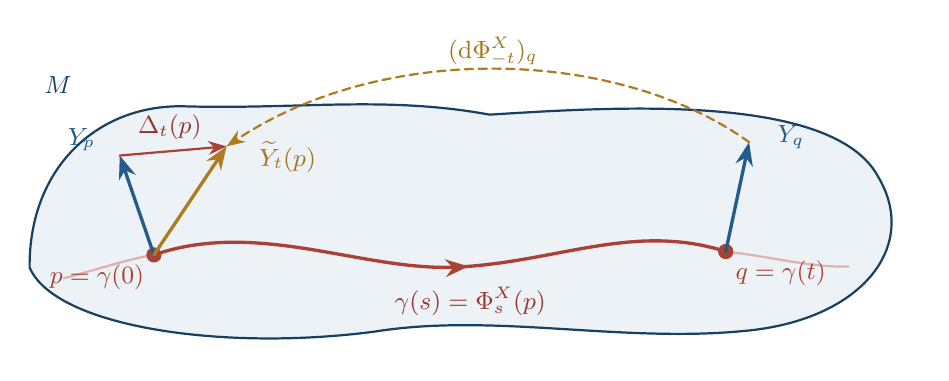
\begin{tikzpicture}[>=Stealth,scale=1.06,line cap=round,line join=round]
% Jedno spójne otoczenie na M; p i q są punktami czerwonej trajektorii.
\filldraw[fill=manifoldblue!8,draw=manifoldblue!70!black,thick]
 (-5.14,-.67) .. controls (-5.15,.52) and (-4.33,1.28) .. (-3.3,1.26)
 .. controls (-1.92,1.22) and (-.88,1.39) .. (.37,1.16)
 .. controls (1.84,1.25) and (4.49,1.43) .. (5.03,.41)
 .. controls (5.52,-.42) and (4.83,-1.3) .. (3.44,-1.43)
 .. controls (1.94,-1.58) and (.42,-1.21) .. (-1.01,-1.44)
 .. controls (-2.84,-1.68) and (-4.84,-1.38) .. cycle;
\node[font=\small,manifoldblue!75!black] at (-4.8,1.51) {$M$};
\coordinate (P) at (-3.65,-.52);
\coordinate (Q) at (3.2,-.48);
% Ciągła krzywa całkowa; wyraźne punkty p, q i kierunek czasu.
\draw[manifoldred!40,thick] (-4.73,-.8)
 .. controls (-4.38,-.71) and (-3.96,-.57) .. (P);
\draw[manifoldred,very thick,postaction={decorate},
 decoration={markings,mark=at position .55 with {\arrow{Stealth}}}]
 (P) .. controls (-2.43,-.1) and (-1.21,-.69) .. (-.1,-.67)
 .. controls (1.13,-.63) and (2.08,-.12) .. (Q);
\draw[manifoldred!40,thick] (Q)
 .. controls (3.81,-.55) and (4.19,-.67) .. (4.67,-.66);
\node[font=\small,manifoldred!85!black] at (.14,-1.08)
 {$\gamma(s)=\Phi_s^X(p)$};
\fill[manifoldred] (P) circle (2.6pt)
 node[below left,font=\small] {$p=\gamma(0)$};
\fill[manifoldred] (Q) circle (2.6pt)
 node[below right,font=\small] {$q=\gamma(t)$};
% Wektory porównywane po sprowadzeniu do T_p M.
\draw[->,manifoldblue,very thick] (P)--(-4.06,.67);
\draw[->,manifoldgold!85!black,very thick] (P)--(-2.78,.78);
\node[font=\small,manifoldblue] at (-4.52,.86) {$Y_p$};
\node[font=\small,manifoldgold!80!black] at (-2.05,.65)
 {$\widetilde Y_t(p)$};
\draw[->,manifoldred,thick] (-4.06,.67)--(-2.78,.78);
\node[font=\small,manifoldred!85!black] at (-3.46,1.01) {$\Delta_t(p)$};
% Wektor Y_q oraz schemat cofnięcia jego wartości, odrębny od trajektorii.
\draw[->,manifoldblue,very thick] (Q)--(3.48,.83);
\node[font=\small,manifoldblue] at (3.98,.89) {$Y_q$};
\draw[->,manifoldgold!85!black,thick,densely dashed]
 (3.48,.83) .. controls (1.93,1.95) and (-.88,2.05) .. (-2.78,.78);
\node[font=\small,manifoldgold!80!black] at (.41,1.92)
 {$(\dd\Phi_{-t}^X)_q$};
\end{tikzpicture}
\caption{Punkty $p=\gamma(0)$ i $q=\gamma(t)=\Phi_t^X(p)$ leżą
na tej samej krzywej całkowej na $M$; czerwona strzałka pokazuje
ruch w czasie od $p$ do $q$. Wektor $Y_q$ cofamy różniczką
przepływu do $T_pM$, otrzymując $\widetilde Y_t(p)$.
Tam porównujemy go z $Y_p$; $\Delta_t(p)$ jest ich różnicą.
Przerywana strzałka przedstawia transport wektora, nie ruch punktu.}
\label{fig:pochodna-liego}
\end{figure}

Dokładnie, oznaczając $q=\Phi_t^X(p)$, mamy
\[
 \widetilde Y_t(p):=(\dd\Phi_{-t}^X)_qY_q\in T_pM,\qquad
 (\Lie_XY)_p=\lim_{t\to0}\frac{\widetilde Y_t(p)-Y_p}{t}.
\]
Dla każdego małego $t$ oba odejmowane wektory leżą w $T_pM$.
Rysunek~\ref{fig:pochodna-liego} pokazuje różnicę $\Delta_t(p)$,
której iloraz przez $t$ ma granicę dla $t\to0$.


\begin{twierdzenie}\label{thm:lie-nawias}
Dla dowolnych pól $X,Y$ zachodzi
\begin{equation}\label{eq:lie-nawias}
 \Lie_XY=[X,Y].
\end{equation}
Zatem pochodna Liego funkcji jest działaniem derywacji,
a pochodna Liego pola jest nawiasem.
\end{twierdzenie}
\begin{proof}
Ustalmy $p\in M$ i $f\in C^\infty(M)$. Pracujemy w otoczeniu $p$
i dla na tyle małych $|t|$, aby lokalny przepływ $\Phi_t=\Phi_t^X$
oraz $\Phi_{-t}$ były określone we wszystkich rozważanych punktach.
Z definicji cofnięcia pola, przy $q=\Phi_t(p)$,
\[
 Z_t(p):=(\Phi_t^*Y)_p=(\dd\Phi_{-t})_qY_q\in T_pM.
\]
Wektory $Z_t(p)$ leżą więc w \emph{jednej} przestrzeni $T_pM$,
a $Z_0(p)=Y_p$. Aby obliczyć ich pochodną, zadziałajmy nimi
na dowolną funkcję $f$. Definicja różniczki daje
\begin{equation}\label{eq:lie-pullback-funkcja}
 Z_t(p)(f)
 =Y_q(f\circ\Phi_{-t})
 =Y(f\circ\Phi_{-t})(\Phi_t(p)).
\end{equation}
Oznaczmy $F(t,r):=f(\Phi_{-t}(r))$ dla $r$ w otoczeniu $p$.
Ponieważ $\frac{\dd}{\dd t}\Phi_{-t}(r)=-X_{\Phi_{-t}(r)}$,
reguła łańcucha daje
\[
 F(0,r)=f(r),\qquad
 \left.\frac{\partial F}{\partial t}\right|_{(0,r)}
 =-X(f)(r).
\]
Niech $H(t,r):=Y_r(F(t,\cdot))$. Wtedy prawa strona
\eqref{eq:lie-pullback-funkcja} jest równa $H(t,\Phi_t(p))$.
Różniczkując to złożenie, musimy uwzględnić zarówno zmianę
funkcji $H$ z czasem, jak i ruch punktu $\Phi_t(p)$:
\begin{align*}
 \left.\frac{\dd}{\dd t}H(t,\Phi_t(p))\right|_{t=0}
 &=\left.\frac{\partial H}{\partial t}\right|_{(0,p)}
   +X_p\bigl(H(0,\cdot)\bigr) \\
 &=-Y_p\bigl(X(f)\bigr)+X_p\bigl(Y(f)\bigr).
\end{align*}
W drugim kroku użyliśmy $H(0,\cdot)=Y(f)$ oraz
$\partial_tH(0,p)=Y_p\bigl(\partial_tF(0,\cdot)\bigr)$.
Zamiana kolejności $Y$ i $\partial_t$ jest dopuszczalna:
w lokalnych współrzędnych $Y=\sum_iY^i(r)\partial_{r^i}$,
współczynniki $Y^i$ nie zależą od $t$, a funkcja $F$ jest gładka.
Wreszcie, ponieważ $Z_t(p)$ jest gładką krzywą w $T_pM$,
jej pochodną można obliczyć po przyłożeniu do $f$. Otrzymujemy
\[
 (\Lie_XY)_p(f)
 =\left.\frac{\dd}{\dd t}Z_t(p)(f)\right|_{t=0}
 =X(Yf)(p)-Y(Xf)(p)=[X,Y]_p(f).
\]
Równość zachodzi dla każdej funkcji gładkiej $f$. Funkcje gładkie
rozróżniają wektory styczne: wystarczy wziąć funkcje, które
w pobliżu $p$ pokrywają się ze współrzędnymi lokalnymi.
Zatem $(\Lie_XY)_p=[X,Y]_p$; punkt $p$ był dowolny.
\end{proof}

\begin{stwierdzenie}\label{prop:lie-ewolucja}
Na wspólnych dziedzinach lokalnego przepływu pola $X$ zachodzi
\[
 \frac{\dd}{\dd t}\Phi_t^*Y=\Phi_t^*[X,Y].
\]
\end{stwierdzenie}
\begin{proof}
Dla dyfeomorfizmu $F$ cofnięcie pola oznacza $F^*Y=(F^{-1})_*Y$.
Reguła łańcucha daje $(F\circ G)^*=G^*F^*$.
Prawo grupowe przepływu pozwala zatem napisać
$\Phi_{t+h}^*Y=\Phi_t^*(\Phi_h^*Y)$.
Ustalamy punkt i dostatecznie małe wspólne otoczenie, aby
wszystkie te odwzorowania były określone dla $h$ bliskiego zeru.
Różniczkujemy po $h$ w zerze: liniowa mapa cofająca przez
ustalone $\Phi_t$ nie zależy od $h$, a
$\left.\partial_h\right|_0\Phi_h^*Y=[X,Y]$
na mocy Twierdzenia~\ref{thm:lie-nawias}.
\end{proof}

\begin{uwaga}[Ten sam rachunek we współrzędnych]
W lokalnych współrzędnych, zapisując pola jako kolumny funkcji,
gładkość przepływu daje przy $t\to0$
\[
 \Phi_t(x)=x+tX(x)+o(t),\qquad
 \dd\Phi_t|_x=I+t\,\dd X|_x+o(t),
\]
a stąd $\dd\Phi_{-t}|_{\Phi_t(x)}=(\dd\Phi_t|_x)^{-1}
=I-t\,\dd X|_x+o(t)$ oraz
$Y(\Phi_t(x))=Y(x)+t\,\dd Y|_xX(x)+o(t)$.
Po pomnożeniu obu wyrażeń otrzymujemy
\[
 (\Phi_t^*Y)(x)=Y(x)+t\bigl(\dd Y|_xX(x)-\dd X|_xY(x)\bigr)+o(t).
\]
Zatem składowa $j$ pochodnej wynosi
$\sum_i(X^i\partial_iY^j-Y^i\partial_iX^j)$,
co zgadza się ze wzorem na nawias Liego.
\end{uwaga}

\begin{przyklad}[Obliczenie w polu przesunięć]
Dla $X=\partial_x$ i $Y=x\partial_y$ mamy
$\Phi_t(x,y)=(x+t,y)$. W punkcie $q=(x+t,y)$ jest
$Y_q=(x+t)\partial_y$, a cofająca różniczka przesunięcia
działa identycznościowo na wektory. Zatem
\[
 ((\Phi_t)^*Y)_{(x,y)}=(x+t)\partial_y,
 \qquad \Lie_XY=\partial_y.
\]
Nie chodzi o różnicę położeń punktów, tylko o zmianę pola
po przeniesieniu obu wektorów do tej samej przestrzeni stycznej.
\end{przyklad}

\begin{figure}[!htbp]
\centering
\begin{tikzpicture}[>=Stealth,scale=1.12,line cap=round,line join=round]
% Cztery kroki komutatora dla X=\partial_x, Y=(1+x)\partial_y.
\coordinate (P) at (-2,-.68);
\coordinate (A) at (.7,-.68);
\coordinate (B) at (.7,1.04);
\coordinate (C) at (-2,1.04);
\coordinate (Q) at (-2,.04);
\fill[manifoldblue!5] (-2.65,-1.15) rectangle (1.38,1.52);
\draw[manifoldblue!22,thin] (-2.65,-1.15) rectangle (1.38,1.52);
\draw[->,very thick,manifoldblue] (P)--(A)
 node[midway,below,font=\small] {$\Phi_t^X$};
\draw[->,very thick,manifoldgreen] (A)--(B)
 node[midway,right,font=\small] {$\Phi_t^Y$};
\draw[->,very thick,manifoldblue] (B)--(C)
 node[midway,above,font=\small] {$\Phi_{-t}^X$};
\draw[->,very thick,manifoldgreen] (C)--(Q)
 node[midway,left,font=\small] {$\Phi_{-t}^Y$};
\fill[manifoldred] (P) circle (2.5pt) node[below left,font=\small] {$p$};
\fill[manifoldred] (Q) circle (2.5pt) node[left,font=\small] {$C_t(p)$};
\draw[->,thick,manifoldred,densely dashed] (-1.66,-.68)--(-1.66,.04)
 node[midway,right,font=\small] {$t^2[X,Y]_p$};
\node[font=\footnotesize,align=center] at (3.7,.52)
 {$C_t=\Phi_{-t}^Y\circ\Phi_{-t}^X$\\[2pt]
 $\circ\Phi_t^Y\circ\Phi_t^X$};
\node[font=\footnotesize,align=center,text width=3.4cm] at (3.75,-.6)
 {Końcowy punkt leży o rząd $t^2$ ponad początkiem.};
\end{tikzpicture}
\caption{Komutator małych przepływów. Po przejściu kolejno wzdłuż
$X,Y,-X,-Y$ droga zwykle się nie zamyka; wyraz przemieszczenia rzędu $t^2$ jest wyznaczony przez nawias
$[X,Y]$. Jeśli $[X,Y]_p=0$, wyraz rzędu $t^2$ znika;
ewentualny pierwszy niezerowy wyraz ma wyższy rząd.
Rysunek schematycznie ilustruje przykład
$X=\partial_x$, $Y=(1+x)\partial_y$.}
\label{fig:komutator-przeplywow}
\end{figure}

Jeśli $C_t=\Phi_{-t}^Y\circ\Phi_{-t}^X\circ\Phi_t^Y\circ\Phi_t^X$, to
w dowolnej mapie wokół $p$ (i dla małego $t$)
\[
 x(C_t(p))=x(p)+t^2\,\dd x_p([X,Y]_p)+O(t^3).
\]
W przykładzie $X=\partial_x$, $Y=(1+x)\partial_y$ i $p=(0,0)$
można to policzyć dokładnie: $p\to(t,0)\to(t,t+t^2)
\to(0,t+t^2)\to(0,t^2)$. Geometria rysunku zgadza się więc ze
znakiem konwencji~\eqref{eq:nawias-def}.

Uzasadnijmy także wzór ogólny, zamiast wnioskować z jednego przykładu.
W ustalonej mapie przepływ gładkiego pola $Z$ ma rozwinięcie
\[
 \Phi_t^Z(x)=x+tZ(x)+\tfrac12t^2 DZ(x)Z(x)+O(t^3),
\]
bo druga pochodna krzywej całkowej w zerze to $DZ(x)Z(x)$.
Oznaczmy kolejne punkty czterech kroków przez $x_1,\ldots,x_4$.
Rozwijając pola w punktach pośrednich, dostajemy
\begin{align*}
 x_1&=x+tX+\tfrac12t^2 DX\,X+O(t^3),\\
 x_2&=x+t(X+Y)+t^2(\tfrac12 DX\,X+DY\,X+\tfrac12 DY\,Y)+O(t^3),\\
 x_3&=x+tY+t^2(DY\,X+\tfrac12 DY\,Y-DX\,Y)+O(t^3),\\
 x_4&=x+t^2(DY\,X-DX\,Y)+O(t^3).
\end{align*}
Wszystkie pola i ich macierze pochodnych po prawej stronie
są obliczone w $x$. Równość $DY\,X-DX\,Y=[X,Y](x)$
wynika ze wzoru~\eqref{eq:nawias-wspolrzedne}.
Reszty $O(t^3)$ są rozumiane w tej mapie, dla punktów w
dostatecznie małym otoczeniu i małego czasu, gdy złożenia istnieją.


\begin{uwaga}[Znaczenie znaku]
W~\eqref{eq:lie-y} wektor cofamy przez $\Phi_{-t}$.
Przy tej konwencji $\Lie_XY=[X,Y]$. Gdyby transportować
$Y_p$ w przód i porównywać z $Y_{\Phi_t(p)}$ w punkcie
$\Phi_t(p)$ w odwrotnej kolejności, otrzymalibyśmy zapis
z przeciwnym znakiem. Przed rachunkiem warto zawsze ustalić,
które dwa wektory są porównywane i w jakim punkcie.
\end{uwaga}

\section{Pola zależne od czasu i izotopie}
\label{sec:izotopie}

Przepływ pola stałego w czasie spełnia lokalne prawo grupowe;
dla pola zupełnego tworzy jednoparametrową grupę dyfeomorfizmów.
W topologii różniczkowej często trzeba deformować obiekty według
zaplanowanego ruchu, którego prędkość może zmieniać się z czasem.

\begin{definicja}
\emph{Pole zależne od czasu} to rodzina $X_t\in\X(M)$,
$t\in[0,1]$, gładka łącznie w $(t,p)$ (na końcach przedziału
w sensie lokalnego gładkiego przedłużenia). Jej krzywe całkowe spełniają nieautonomiczne równanie
$\gamma'(t)=(X_t)_{\gamma(t)}$. Odwzorowanie ewolucji
$F_{t,s}(p)$ przenosi położenie w chwili $s$ do położenia
w chwili $t$, tam gdzie rozwiązanie istnieje.
\end{definicja}

Dodanie czasu jako zmiennej sprowadza to równanie do autonomicznego
pola $\widehat X=\partial_t+X_t$ na czasoprzestrzeni.
Krzywa tego pola startująca w $(s,p)$ ma postać
$(s+u,F_{s+u,s}(p))$. Twierdzenie~\ref{thm:ode}, zastosowane
lokalnie także do przedłużeń przy końcach przedziału, daje
gładkość ewolucji łącznie w $(t,s,p)$. Jednoznaczność daje prawo
\begin{equation}\label{eq:ewolucja}
 F_{s,s}=\id,\qquad F_{u,t}\circ F_{t,s}=F_{u,s},
 \qquad F_{s,t}=F_{t,s}^{-1}.
\end{equation}
Równości obowiązują tam, gdzie odpowiednie rozwiązania istnieją;
$F_{t,s}$ jest dyfeomorfizmem swojej otwartej dziedziny na obraz,
z odwrotnością $F_{s,t}$.
Zwykle $F_{t,0}$ \emph{nie} spełnia
$F_{t+s,0}=F_{t,0}\circ F_{s,0}$, bo samo pole się zmienia.
Jeżeli nośniki wszystkich $X_t$ mieszczą się w jednym zwartym
$K\subset M$, ewolucja istnieje dla całego przedziału $[0,1]$:
poza $K$ krzywe stałe są rozwiązaniami, a jednoznaczność
w obu kierunkach czasu nie pozwala trajektorii z $K$ wyjść
poza $K$. Trajektoria startująca w $p$ pozostaje więc w
$K\cup\{p\}$. Jej podniesienie do czasoprzestrzeni leży
w zwartym $[0,1]\times(K\cup\{p\})$. Argument przedłużania
z dowodu Twierdzenia~\ref{thm:zupelnosc}, z lokalnymi przedłużeniami
pola na końcach przedziału, wyklucza skończony czas zakończenia
rozwiązania przed dojściem do wymaganej chwili. Istotny jest
\emph{wspólny} zwarty nośnik, a nie tylko zwartość każdego z nośników osobno.

\begin{definicja}
Gładka rodzina dyfeomorfizmów $h_t\colon M\to M$ z
$h_0=\id_M$ to \emph{izotopia otoczenia}.
Gładka rodzina zanurzeń $i_t\colon N\hookrightarrow M$ to
\emph{izotopia zanurzeń}. Drugie pojęcie dotyczy tylko ruchu
podrozmaitości, pierwsze przesuwa całe otoczenie.
Zanurzenie rozumiemy jak w Rozdziale~\ref{ch:rozmaitosci}:
jest to immersja będąca homeomorfizmem na obraz.
Nośnikiem izotopii otoczenia nazywamy domknięcie zbioru
$\{p\in M:h_t(p)\ne p\text{ dla pewnego }t\in[0,1]\}$.
\end{definicja}

Każda izotopia otoczenia jest generowana przez pole zależne od
czasu: dla $q=h_t(p)$ kładziemy
\begin{equation}\label{eq:generator-izotopii}
 (X_t)_q=\left.\frac{\partial h_t(p)}{\partial t}
 \right|_{p=h_t^{-1}(q)}.
\end{equation}
Gładkość tego pola wymaga także gładkości $(t,q)\mapsto h_t^{-1}(q)$.
Wynika ona z twierdzenia o funkcji odwrotnej zastosowanego do
$H(t,p)=(t,h_t(p))$: różniczka jest blokowo trójkątna z
odwracalnymi blokami $1$ i $\dd h_t$. Przy $t=0,1$ stosujemy
lokalne przedłużenia; pierwsza współrzędna pozostaje czasem.
Jednoznaczność rozwiązań daje $h_t=F_{t,0}$.
W szczególności pole zależne od czasu
o wspólnym zwartym nośniku buduje izotopię otoczenia
stałą poza tym nośnikiem.

\begin{twierdzenie}[Rozszerzenie izotopii, wersja zwarta]
\label{thm:rozszerzenie-izotopii}
Niech $M$ będzie rozmaitością bez brzegu,
$N$ jej zwartą podrozmaitością bez brzegu,
a $i_t\colon N\hookrightarrow M$, $t\in[0,1]$, gładką
izotopią zanurzeń. Istnieje izotopia otoczenia $h_t$ taka, że
$h_t\circ i_0=i_t$. Jej nośnik można umieścić w dowolnym
otwartym otoczeniu zwartego śladu
$\bigcup_{t\in[0,1]}i_t(N)$.
\end{twierdzenie}
\begin{proof}
\emph{Krok 1: pole na śladzie izotopii.}
Zbudujmy \emph{ślad w czasoprzestrzeni}
\[
 \mathcal T:=\{(t,i_t(x)):t\in[0,1],\ x\in N\}
 \subset[0,1]\times M.
\]
Odwzorowanie $I(t,x)=(t,i_t(x))$ jest różnowartościowe:
z równości pierwszych współrzędnych mamy ten sam $t$,
a różnowartościowość $i_t$ daje ten sam $x$.
Jego różniczka jest injektywna: jeśli
$\dd I_{(t,x)}(a,v)=0$, to pierwsza współrzędna daje
$a=0$, a następnie $\dd (i_t)_x(v)=0$ wymusza $v=0$.
Ponieważ $[0,1]\times N$ jest zwarta, $I$ jest zanurzeniem
(ciągła bijekcja z przestrzeni zwartej na podprzestrzeń
Hausdorffa ma ciągłą odwrotność). Zatem $\mathcal T$
jest zwartą podrozmaitością z brzegiem w $[0,1]\times M$.
Wyjaśnijmy postać lokalną także dla $t=0,1$. W lokalnych
współrzędnych $u$ na $N$ wybieramy $k=\dim N$ składowych $i_t(u)$,
których różniczka względem $u$ jest odwracalna. Odwzorowanie
$(t,u)\mapsto(t,i_t^1(u),\ldots,i_t^k(u))$ jest lokalnym
dyfeomorfizmem. Pozostałe składowe śladu są więc wykresem
$w=b(t,z)$. Zmiana $(t,z,w)\mapsto(t,z,w-b(t,z))$ prostuje
ślad i zachowuje czas, a zatem również brzeg przy $t=0,1$.
Homeomorficzność $I$ na obraz pozwala zmniejszyć otoczenie tak,
aby nie zawierało innych fragmentów śladu.
Wzdłuż niej mamy dobrze określony \emph{pionowy} wektor
\[
 V(t,i_t(x)):=\frac{\partial i_t(x)}{\partial t}
 \in T_{i_t(x)}M.
\]
Jest gładki, bo $I$ ma gładką odwrotność na $\mathcal T$.

\emph{Krok 2: przedłużenie o małym nośniku.}
Niech $O\subset M$ będzie wskazanym otwartym otoczeniem
rzutu $\mathcal T$ na $M$. Wokół każdego punktu
$\mathcal T$ wybieramy lokalne współrzędne na
$[0,1]\times M$, w których $\mathcal T$ ma postać
normalną opisaną powyżej; otoczenia wybieramy wewnątrz
$[0,1]\times O$. W lokalnej trywializacji $TM$
składowe wektora $V$ są gładkimi funkcjami współrzędnych
na $\mathcal T$; przedłużamy je, nadając im te same
wartości w pobliskich kierunkach normalnych.
Otrzymujemy lokalne pola pionowe $V^{(j)}$, których
ograniczenia do $\mathcal T$ są równe $V$.
Zwartość $\mathcal T$ pozwala wybrać skończenie wiele
takich otoczeń i nieujemne gładkie funkcje odcinające $\chi_j$
o zwartych nośnikach w tych otoczeniach, z
$\sum_j\chi_j>0$ na $\mathcal T$.
Na otwartym zbiorze $U=\{\sum_j\chi_j>0\}$ kładziemy
$Y=(\sum_j\chi_j V^{(j)})/(\sum_k\chi_k)$,
przedłużając każde $\chi_j V^{(j)}$ przez zero poza jego otoczenie.
Na $\mathcal T$ wszystkie składniki $V^{(j)}$ są równe
$V$, więc $Y|_{\mathcal T}=V$.
Wybieramy jeszcze funkcję odcinającą $\rho$ równą $1$ w
otoczeniu zwartej $\mathcal T$, o zwartym nośniku
w $U\subset[0,1]\times O$, i mnożymy przez nią $Y$.
Taka funkcja powstaje ze skończonego pokrycia $\mathcal T$
otoczeniami z funkcjami $0\le\rho_j\le1$, równymi $1$
na mniejszych otoczeniach: $\rho=1-\prod_j(1-\rho_j)$.
Przy końcach czasu wystarczą ograniczenia zwykłych funkcji
odcinających do półprzestrzeni. Warunek $\supp\rho\subset U$
zapewnia, że nie dzielimy przez zero.
Przedłużenie przez zero definiuje gładkie pole $X_t$
na całym $M$, gładkie w $t$, którego wszystkie nośniki
leżą w jednym zwartym $K\subset O$ (rzucie $\supp\rho$ na $M$)
i które spełnia
$(X_t)_{i_t(x)}=\partial_t i_t(x)$.

\emph{Krok 3: całkowanie.} Każda krzywa
$t\mapsto i_t(x)$ spełnia równanie
$\dot q(t)=(X_t)_{q(t)}$ z warunkiem początkowym
$q(0)=i_0(x)$. Lokalna jednoznaczność dla pola zależnego
od czasu wynika z tego samego argumentu co
Twierdzenie~\ref{thm:ode}, po dodaniu czasu jako zmiennej.
Wspólny zwarty nośnik $K$ wyklucza ucieczkę rozwiązania
w skończonym czasie, więc ewolucja $F_{t,s}$ istnieje
dla $s,t\in[0,1]$. Z jednoznaczności
$F_{t,0}(i_0(x))=i_t(x)$. Kładąc $h_t:=F_{t,0}$,
otrzymujemy izotopię dyfeomorfizmów:
jej odwrotnością w chwili $t$ jest $F_{0,t}$.
Poza $K$ pole $X_t$ znika, zatem punkty tam pozostają
nieruchome i nośnik $h_t$ leży w $O$.
\end{proof}

\begin{przyklad}[Przesuwanie punktu]
Gdy $i_t\colon\{*\}\hookrightarrow M$ opisuje gładką drogę
$p_t$ w spójnej składowej $M$, rozszerzenie izotopii daje
rodzinę dyfeomorfizmów $h_t$ z $h_t(p_0)=p_t$.
Można ją zbudować konkretnie, przedłużając prędkość
$\dot p_t$ do pola wspieranego w małym otoczeniu całej drogi.
To narzędzie pozwala przesuwać lokalne konstrukcje
bez zmieniania odległych części rozmaitości.
\end{przyklad}

\begin{uwaga}[Kołnierz brzegu]
Jeśli $M$ ma zwarty brzeg, wybieramy pole $X$, które na
$\partial M$ jest skierowane do wnętrza i poprzeczne do brzegu.
Jego mały dodatni przepływ daje dyfeomorfizm na obraz
$\partial M\times[0,\varepsilon)\to M$,
$(p,t)\mapsto\Phi_t(p)$, zwany \emph{kołnierzem}.
Pole takie otrzymujemy z lokalnych pól skierowanych do wnętrza
przez nieujemne funkcje odcinające; dodatnia składowa normalna
pozostaje dodatnia przy ich sumowaniu. W mapach półprzestrzeni
przedłużamy pole za brzeg, aby zastosować lokalne twierdzenie
o przepływie. Jego dodatnie trajektorie pozostają początkowo w $M$.
Różniczka $(v,a)\mapsto v+aX_p$ jest izomorfizmem w $(p,0)$.
Twierdzenie o funkcji odwrotnej, z uwzględnieniem znaku składowej
normalnej, daje lokalny dyfeomorfizm półotoczeń. Zwartość brzegu
pozwala wybrać wspólny czas istnienia i lokalnej odwracalności.
Pozostaje globalna injektywność dla małego czasu. Gdyby żadna
wartość $\varepsilon$ jej nie dawała, istniałyby różne pary
$(p_j,t_j),(q_j,s_j)$ o tym samym obrazie i $0\le t_j,s_j<1/j$.
Po przejściu do podciągu $p_j\to p$, $q_j\to q$; ciągłość
daje $p=q$. Obie pary leżą wtedy w jednym otoczeniu lokalnej
injektywności przy $(p,0)$, sprzeczność. Obraz jest otwartym
otoczeniem brzegu w $M$, bo mapa jest lokalnym dyfeomorfizmem
półotoczeń. Kołnierz pozwala opisywać otoczenie brzegu
współrzędnymi niezależnymi od punktu na brzegu.
\end{uwaga}

\par\smallskip
{\footnotesize\noindent\emph{Dalsza lektura:}
\href{https://doi.org/10.1007/978-1-4419-9982-5}
{J. M. Lee, \emph{Introduction to Smooth Manifolds}, wyd. 2},
rozdziały 8--9: pola, przepływy (także przy brzegu),
pochodna Liego i pola zależne od czasu;
rozdział 12: rozszerzenie pochodnej Liego na pola tensorowe;
\href{https://people.dm.unipi.it/benedett/MILNOR-TDVPOINT.pdf}
{J. Milnor, \emph{Topology from the Differentiable Viewpoint}},
§4, s.~20--24: gładka izotopia i przemieszczanie punktów
przez przepływ; §6, s.~32--41: pola wektorowe i liczba Eulera.\par}
\clearpage

\chapter{Algebra tensorowa i zewnętrzna}
\label{ch:algebra-tensorowa}
\index{tensor}

Wektor styczny i kowektor z Rozdziału~\ref{ch:rozmaitosci} są obiektami
liniowymi. Do opisu odwzorowań wieloliniowych, operatorów i
wyznaczników potrzebujemy przestrzeni, w której symbole
$v\otimes w$ spełniają dokładnie relacje wymuszone przez dwuliniowość.
Zbudujemy ją bez wyboru bazy, a dopiero potem wyprowadzimy rachunek
współrzędnych. W całym rozdziale $\mathbb K=\R$ albo $\C$;
przestrzenie mają skończony wymiar, chyba że zaznaczono inaczej.
W przypadku zespolonym wszystkie odwzorowania wieloliniowe są
$\C$-liniowe w każdym argumencie: nie stosujemy tu sprzężenia
zespolonego. W szczególności dualność algebraiczna nie jest
utożsamieniem przez iloczyn hermitowski.

\section{Iloczyn tensorowy: definicja, istnienie i jednoznaczność}
\label{sec:iloczyn-tensorowy}

\begin{definicja}[Własność uniwersalna]
\index{wlasnosc uniwersalna@Własność uniwersalna}
\label{def:tensor-universal}
\emph{Iloczynem tensorowym} przestrzeni $V,W$ nazywamy parę
$(T,\tau)$, gdzie $T$ jest przestrzenią liniową,
$\tau\colon V\times W\to T$ jest odwzorowaniem dwuliniowym,
a dla każdej przestrzeni $Z$ i każdego odwzorowania dwuliniowego
$B\colon V\times W\to Z$ istnieje dokładnie jedno odwzorowanie
liniowe $\widetilde B\colon T\to Z$ takie, że
$B=\widetilde B\circ\tau$. Piszemy $T=V\otimes W$ i
$\tau(v,w)=v\otimes w$. Elementy $v\otimes w$ nazywamy
\emph{tensorami prostymi}.
\end{definicja}

\begin{center}
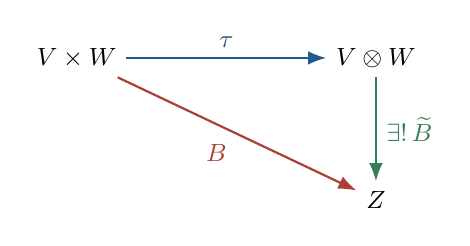
\begin{tikzpicture}[>=Latex, every node/.style={font=\small}]
 \node (vw) at (0,1.8) {$V\times W$};
 \node (tensor) at (3.8,1.8) {$V\otimes W$};
 \node (z) at (3.8,0) {$Z$};
 \draw[->,thick,manifoldblue] (vw) -- node[above] {$\tau$} (tensor);
 \draw[->,thick,manifoldred] (vw) -- node[below left] {$B$} (z);
 \draw[->,thick,manifoldgreen] (tensor) -- node[right] {$\exists!\,\widetilde B$} (z);
\end{tikzpicture}
\end{center}

Samo zapisanie $v\otimes w$ nie jest definicją: najpierw trzeba
wykazać, że przestrzeń o tej własności istnieje.

\begin{uwaga}[Co znaczy ,,formalna kombinacja liniowa''?]
\label{rem:kombinacje-formalne}
Jeśli $S$ jest dowolnym zbiorem, \emph{wolna przestrzeń liniowa}
o bazie symboli $[s]$, $s\in S$, składa się z zapisów
\[
 \sum_{s\in S} c_s[s],\qquad c_s\in\mathbb K,
 \quad c_s=0\text{ poza skończoną liczbą indeksów}.
\]
To jest kombinacja \emph{formalna}: dodajemy współczynniki
stojące przy tym samym symbolu i mnożymy je przez skalary,
ale nie przypisujemy symbolom żadnych innych relacji.
Dwa takie zapisy są równe dokładnie wtedy, gdy ich
współczynniki przy każdym $[s]$ są równe. W szczególności
$[s]$ i $[s']$ są niezależnymi wektorami, jeśli $s\ne s'$.
Można myśleć o takim zapisie jako o funkcji
$s\mapsto c_s$ o \emph{skończonym nośniku}.

W dowodzie poniżej bierzemy $S=V\times W$. Jeśli
$v,v'$ są niezależne, symbole $[(v+v',w)]$, $[(v,w)]$
i $[(v',w)]$ mają różne indeksy, więc przed podzieleniem
przez relacje są niezależne. Dopiero iloraz nakazuje równość
$[(v+v',w)]+R=[(v,w)]+[(v',w)]+R$.
Równość dwóch klas $x+R=y+R$ oznacza dokładnie $x-y\in R$.
Ta ostatnia reguła wyjaśnia, dlaczego relacje dwuliniowości
pojawiają się w konstruowanej przestrzeni, a nie były
ukrytym założeniem o symbolach.
\end{uwaga}

\begin{twierdzenie}[Konstrukcja iloczynu tensorowego]
\label{thm:tensor-istnienie}
Dla dowolnych przestrzeni liniowych $V,W$ iloczyn tensorowy istnieje.
Ponadto tensory proste rozpinają $V\otimes W$.
\end{twierdzenie}
\begin{proof}
Niech $F$ będzie wolną przestrzenią liniową o bazie formalnych
symboli $[(v,w)]$, po jednym dla każdej pary $(v,w)\in V\times W$.
Jej elementy są kombinacjami z Uwagi~\ref{rem:kombinacje-formalne}.
Ta pomocnicza przestrzeń jest na ogół nieskończenie wymiarowa,
nawet gdy $V,W$ mają skończony wymiar; dopiero iloraz narzuci relacje.
Niech $R\subseteq F$ będzie podprzestrzenią rozpiętą przez
wszystkie elementy czterech rodzajów:
\begin{align*}
 &[(v+v',w)]-[(v,w)]-[(v',w)],
 &&[(av,w)]-a[(v,w)],\\
 &[(v,w+w')]-[(v,w)]-[(v,w')],
 &&[(v,aw)]-a[(v,w)],
\end{align*}
gdzie $a\in\mathbb K$. Kładziemy $T:=F/R$ oraz
$v\otimes w:=[(v,w)]+R$. Cztery relacje pokazują kolejno,
że $\tau(v,w):=v\otimes w$ jest liniowa w każdej zmiennej.
Każda klasa w $F/R$ jest skończoną kombinacją liniową klas $[(v,w)]+R$,
więc tensory proste rozpinają $T$.

Weźmy teraz dowolne odwzorowanie dwuliniowe $B\colon V\times W\to Z$.
Na $F$ istnieje dokładnie jedno odwzorowanie liniowe
$L\colon F\to Z$ o wartościach $L([(v,w)])=B(v,w)$:
określamy je na bazie i przedłużamy liniowo. Dwuliniowość $B$
oznacza, że $L$ zeruje każdy z czterech typów generatorów $R$,
a więc $R\subseteq\ker L$. Odwzorowanie $L$ przechodzi na iloraz:
$\widetilde B(x+R):=L(x)$ dla $x\in F$. Jest dobrze określone, bo
$x+R=x'+R$ implikuje $L(x-x')=0$, i spełnia
$\widetilde B(v\otimes w)=B(v,w)$. Jeśli drugie odwzorowanie liniowe
spełniałoby tę samą równość, zgadzałoby się z $\widetilde B$
na zbiorze rozpinającym $T$, a zatem wszędzie.
\end{proof}

\begin{uwaga}[Faktoryzacja przez iloraz a izomorfizm]
\label{rem:tensor-iloraz-izomorfizm}
W dowodzie wystarczyło $R\subseteq\ker L$, aby otrzymać
odwzorowanie $\widetilde B:F/R\to Z$. To jest ten sam mechanizm
przechodzenia do ilorazu, który w ogólnej postaci
porządkuje Twierdzenie~\ref{thm:modul-izomorfizm}
w Rozdziale~\ref{ch:algebra-abstrakcyjna}
(przestrzenie liniowe są modułami nad $\mathbb K$).
Pełne twierdzenie daje $F/\ker L\cong\operatorname{im}L$.
Nie utożsamiamy natomiast $F/R$ z $\operatorname{im}L$,
chyba że $R=\ker L$; do istnienia iloczynu tensorowego
taka równość nie jest potrzebna.
\end{uwaga}

\begin{twierdzenie}[Jednoznaczność]
\label{thm:tensor-jednoznacznosc}
Jeżeli $(T,\tau)$ i $(T',\tau')$ spełniają
Definicję~\ref{def:tensor-universal}, istnieje dokładnie jeden
izomorfizm spełniający
\[
 J\colon T\to T',\qquad J\circ\tau=\tau'.
\]
\end{twierdzenie}
\begin{proof}
Własność uniwersalna $(T,\tau)$ zastosowana do $\tau'$ daje
jedyne odwzorowanie liniowe $J\colon T\to T'$ z~żądaną własnością.
Podobnie $(T',\tau')$ daje $K\colon T'\to T$ z
$K\circ\tau'=\tau$. Zatem $(KJ)\circ\tau=\tau$.
Również $\id_T\circ\tau=\tau$; jednoznaczność faktoryzacji
przez $T$ wymusza $KJ=\id_T$. Tak samo $JK=\id_{T'}$.
Odwzorowanie $J$ jest więc izomorfizmem i jedynym możliwym odwzorowaniem
zachowującym wskazane obrazy par $(v,w)$.
\end{proof}

W szczególności
\begin{equation}\label{eq:tensor-biliniowosc}
 (av+bv')\otimes w=a(v\otimes w)+b(v'\otimes w),\qquad
 v\otimes(aw+bw')=a(v\otimes w)+b(v\otimes w').
\end{equation}
\emph{Każdy} element $V\otimes W$ jest skończoną sumą tensorów
prostych, ale nie musi sam być tensorem prostym.

\section{Baza, wymiar i wiele czynników}
\label{sec:baza-tensorowa}

\begin{twierdzenie}[Baza iloczynu tensorowego]
\label{thm:baza-tensorowa}
Jeżeli $e_1,\ldots,e_m$ jest bazą $V$, a
$f_1,\ldots,f_n$ bazą $W$, to
\[
 \bigl\{e_i\otimes f_j:1\leq i\leq m,\;1\leq j\leq n\bigr\}
\]
jest bazą $V\otimes W$. W szczególności
$\dim(V\otimes W)=mn$.
\end{twierdzenie}
\begin{proof}
Dla $v=\sum_i a_i e_i$ i $w=\sum_j b_j f_j$ dwuliniowość daje
\[
 v\otimes w=\sum_{i=1}^m\sum_{j=1}^n a_ib_j(e_i\otimes f_j).
\]
Ponieważ tensory proste rozpinają $V\otimes W$, wyświetlone
wektory są układem rozpinającym. Dla liniowej niezależności
wprowadźmy przestrzeń $\mathbb K^{m\times n}$ z bazą jednostek
macierzowych $E_{ij}$: jedynka na miejscu $(i,j)$ i zera poza nim. Przypisanie
$B(v,w)=(a_i b_j)_{i,j}$ jest dwuliniowe; własność uniwersalna
daje $\widetilde B\colon V\otimes W\to\mathbb K^{m\times n}$
z $\widetilde B(e_i\otimes f_j)=E_{ij}$. Jeśli
$\sum_{i,j}c_{ij}e_i\otimes f_j=0$, zastosowanie
$\widetilde B$ daje $\sum_{i,j}c_{ij}E_{ij}=0$, czyli
wszystkie $c_{ij}=0$. Tak wykazaliśmy również podany wymiar.
\end{proof}

\begin{przyklad}[Tensor prosty a suma tensorów]
Dla $V=W=\R^2$ odwzorowanie z dowodu przypisuje
$(1,2)\otimes(3,-1)$ macierz
$\begin{psmallmatrix}3&-1\\6&-2\end{psmallmatrix}$.
Każdy niezerowy tensor prosty ma tu macierz rzędu $1$:
jest ona iloczynem kolumny współrzędnych $v$ i wiersza
współrzędnych $w$. Natomiast
$e_1\otimes e_1+e_2\otimes e_2$ odpowiada macierzy
identycznościowej rzędu $2$, więc nie jest prosty.
Należy też pamiętać, że $v\otimes w$ nie oznacza pary $(v,w)$:
na przykład $(2v)\otimes w=v\otimes(2w)$.
\end{przyklad}

\begin{stwierdzenie}[Łączność i przestawianie czynników]
\label{prop:tensor-lacznosc}
Istnieją kanoniczne izomorfizmy
\[
 (V\otimes W)\otimes U\longrightarrow V\otimes(W\otimes U),
 \quad (v\otimes w)\otimes u\longmapsto v\otimes(w\otimes u),
\]
\[
 V\otimes W\longrightarrow W\otimes V,
 \quad v\otimes w\longmapsto w\otimes v.
\]
Dlatego możemy pisać $V_1\otimes\cdots\otimes V_k$ bez nawiasów.
\end{stwierdzenie}
\begin{proof}
Odwzorowanie $(v,w,u)\mapsto v\otimes(w\otimes u)$ jest
trójliniowe. Każde odwzorowanie trójliniowe na $V\times W\times U$
faktoryzuje jednoznacznie przez $(V\otimes W)\otimes U$:
najpierw przy ustalonym $u$ faktoryzujemy względem $(v,w)$;
otrzymane odwzorowania $(V\otimes W)\to Z$ zależą liniowo od $u$,
co sprawdzamy na rozpinających $v\otimes w$. Następnie
faktoryzujemy powstałe odwzorowanie dwuliniowe
$(V\otimes W)\times U\to Z$. Otrzymujemy zatem odwzorowanie w treści
stwierdzenia. Analogiczna konstrukcja w drugą stronę daje
$v\otimes(w\otimes u)\mapsto(v\otimes w)\otimes u$.
Oba złożenia są identycznością na tensorach prostych trzech
czynników, które rozpinają odpowiednie przestrzenie.
Izomorfizm przestawiający dwa czynniki pochodzi z dwuliniowego
odwzorowania $(v,w)\mapsto w\otimes v$; jego odwrotność powstaje
po ponownym przestawieniu.
Przy większej liczbie czynników dowolne dwa sposoby zmiany
nawiasowania dają to samo odwzorowanie: na każdym tensorze
prostym zachowują kolejność i wartości wszystkich czynników,
a takie tensory rozpinają dziedzinę. To uzasadnia pomijanie
nawiasów również dla czterech i więcej przestrzeni.
\end{proof}

Kładziemy $V^{\otimes0}:=\mathbb K$ oraz
$V^{\otimes k}:=V\otimes\cdots\otimes V$ dla $k\geq1$.
Jeżeli $\dim V=n$, iterowanie Twierdzenia~\ref{thm:baza-tensorowa}
daje bazę $e_{i_1}\otimes\cdots\otimes e_{i_k}$ i wymiar
\begin{equation}\label{eq:dim-potega-tensorowa}
 \dim V^{\otimes k}=n^k\qquad(k\geq0).
\end{equation}
Dla $k=0$ jest to konwencja $n^0=1$, również gdy $V=0$.

\section{Tensory mieszane i operacje na nich}
\label{sec:operacje-tensorowe}

Oznaczmy $V^*:=\operatorname{Hom}_{\mathbb K}(V,\mathbb K)$.
Jest to przestrzeń liniowych funkcjonałów, zwanych kowektorami.
Dla nieujemnych $r,s$ przyjmujemy konwencję
\begin{equation}\label{eq:typ-tensora}
 T^r_s(V):=V^{\otimes r}\otimes(V^*)^{\otimes s}.
\end{equation}
Tensory typu $(r,s)$ mają $r$ czynników wektorowych i $s$
kowektorowych; powiązane z nimi funkcje wieloliniowe
przyjmują $r$ kowektorów i $s$ wektorów. Na tensorze prostym
wyznacza je wzór
\[
 (v_1\otimes\cdots\otimes v_r\otimes
 \alpha_1\otimes\cdots\otimes\alpha_s)
 (\xi_1,\ldots,\xi_r;w_1,\ldots,w_s)
 =\prod_{a=1}^r\xi_a(v_a)\prod_{b=1}^s\alpha_b(w_b).
\]
Puste iloczyny mają wartość $1$. Dla $r=s=0$ mamy
$T^0_0(V)=\mathbb K$; odwzorowanie bez argumentów określa po prostu
skalar (dziedziną jest jednoelementowy zbiór pustych układów).

\begin{twierdzenie}[Postać wieloliniowa tensora]
\label{thm:tensor-wieloliniowy}
Dla skończenie wymiarowej przestrzeni $V$ powyższy wzór daje
izomorfizm
\[
 T^r_s(V)\cong
 \operatorname{Mult}\bigl((V^*)^r\times V^s,\mathbb K\bigr).
\]
Jeśli $e_1,\ldots,e_n$ jest bazą $V$ i $e^1,\ldots,e^n$
bazą dualną, każdy tensor ma dokładnie jedno rozwinięcie
\begin{equation}\label{eq:wspolczynniki-tensora}
 T=\sum_{\substack{i_1,\ldots,i_r\\j_1,\ldots,j_s}}
 T^{i_1\cdots i_r}{}_{j_1\cdots j_s}
 e_{i_1}\otimes\cdots\otimes e_{i_r}
 \otimes e^{j_1}\otimes\cdots\otimes e^{j_s}.
\end{equation}
\end{twierdzenie}
\begin{proof}
Rozwinięcie i jego jednoznaczność wynikają z kolejnych
zastosowań Twierdzenia~\ref{thm:baza-tensorowa}. Wzór
na działanie na argumentach jest wieloliniowy w czynnikach
tensora, więc przez własność uniwersalną definiuje odwzorowanie liniowe
$T^r_s(V)$ do wskazanej przestrzeni funkcji. Aby wykazać jego
iniektywność, podstawmy w miejsce argumentów elementy baz:
\[
 e^{i_1},\ldots,e^{i_r};\qquad e_{j_1},\ldots,e_{j_s}.
\]
Uzyskana wartość jest dokładnie współczynnikiem
$T^{i_1\cdots i_r}{}_{j_1\cdots j_s}$. Jeśli wszystkie wartości
są zerowe, znikają więc wszystkie współczynniki.
Odwrotnie, dla dowolnej funkcji wieloliniowej $F$ wstawmy te
wartości do prawej strony~\eqref{eq:wspolczynniki-tensora}.
Otrzymany tensor ma te same wartości co $F$ na wszystkich
układach elementów bazowych. Rozwinięcie argumentów i ich
wieloliniowość dają równość na dowolnych argumentach.
\end{proof}

Przykładowo $T^0_2(V)$ to formy dwuliniowe na $V$.
Związek tensorów z operatorami wymaga pilnowania,
z której przestrzeni operator \emph{przyjmuje} argument.

\begin{twierdzenie}[Tensory i przestrzenie operatorów]
\label{thm:tensor-hom}
Dla skończenie wymiarowych $V,W$ istnieje kanoniczny izomorfizm
\begin{equation}\label{eq:tensor-hom}
 \Theta_{V,W}\colon V\otimes W^*\longrightarrow
 \operatorname{Hom}_{\mathbb K}(W,V),\qquad
 \Theta_{V,W}(v\otimes\lambda)(w):=\lambda(w)v.
\end{equation}
W szczególności po zamianie nazw przestrzeni otrzymujemy
$W\otimes V^*\cong\operatorname{Hom}_{\mathbb K}(V,W)$.
\end{twierdzenie}
\begin{proof}
Dla ustalonego $w\in W$ wyrażenie $\lambda(w)v$ zależy
liniowo od $v$ oraz liniowo od $\lambda$; samo przypisanie
$w\mapsto\lambda(w)v$ jest liniowe. Dlatego odwzorowanie
$(v,\lambda)\mapsto(w\mapsto\lambda(w)v)$ ma wartości
w $\operatorname{Hom}(W,V)$ i jest dwuliniowe.
Własność uniwersalna iloczynu tensorowego wyznacza
\emph{jedno} odwzorowanie liniowe $\Theta_{V,W}$ o wzorze
\eqref{eq:tensor-hom}. Tym samym wzór działa również
na sumach: $\Theta_{V,W}(\sum_a v_a\otimes\lambda_a)(w)
=\sum_a\lambda_a(w)v_a$. Nie musimy wybierać sposobu
zapisania takiej sumy, bo $\Theta_{V,W}$ została zdefiniowana
na całej przestrzeni tensorowej.

Zbudujmy odwrotność. Wybierzmy bazę $f_1,\ldots,f_m$
przestrzeni $W$ i jej bazę dualną $f^1,\ldots,f^m$.
Dla $A\in\operatorname{Hom}(W,V)$ połóżmy
\begin{equation}\label{eq:hom-tensor-odwrotna}
 \mathcal I(A):=\sum_{j=1}^m A(f_j)\otimes f^j\in V\otimes W^*.
\end{equation}
Sprawdzimy oba złożenia. Jeśli $w\in W$, to
\[
 \Theta_{V,W}(\mathcal I(A))(w)
 =\sum_j f^j(w)A(f_j)
 =A\!\left(\sum_j f^j(w)f_j\right)=A(w),
\]
bo $w=\sum_j f^j(w)f_j$. Odwrotnie, dla prostego
tensora $v\otimes\lambda$ mamy
\[
 \mathcal I(\Theta_{V,W}(v\otimes\lambda))
 =\sum_j\lambda(f_j)v\otimes f^j
 =v\otimes\left(\sum_j\lambda(f_j)f^j\right)
 =v\otimes\lambda.
\]
Tensory proste rozpinają $V\otimes W^*$, więc drugie
złożenie też jest identycznością wszędzie. Wzór
\eqref{eq:hom-tensor-odwrotna} wygląda zależnie od bazy,
ale jest odwrotnością kanonicznej $\Theta_{V,W}$;
dlatego jego wynik od bazy nie zależy.
\end{proof}

Przy $W=V$ otrzymujemy
$T^1_1(V)=V\otimes V^*\cong\operatorname{End}(V)$.
Na tensorze prostym odpowiada temu wzór
\begin{equation}\label{eq:endo-tensor}
 v\otimes\alpha\longmapsto
 \bigl(w\longmapsto\alpha(w)v\bigr).
\end{equation}
Na przykład $e_i\otimes e^j$ przechodzi na jednostkę
macierzową $E_{ij}$: wysyła $e_j$ na $e_i$, a pozostałe
wektory bazowe na zero. W bazie $e'_i=\sum_a A^a{}_i e_a$
macierz operatora $S$ ma postać $[S]'=A^{-1}[S]A$:
zmieniają się współczynniki, nie sam operator.
Istotnie, jeśli $[v]$ i $[v]'$ oznaczają kolumny współrzędnych,
to $[v]=A[v]'$. Stąd $[Sv]'=A^{-1}[S]A[v]'$.
Baza dualna zmienia się według
$e'^i=\sum_b(A^{-1})^i{}_b e^b$, co wynika z warunku
$e'^i(e'_j)=\delta^i_j$; używamy odwrotności bez sprzężenia zespolonego.

\begin{uwaga}[Funkcja dwuliniowa a operator]
\label{rem:mult-hom}
Z Twierdzenia~\ref{thm:tensor-wieloliniowy} dla typu $(1,1)$
dostajemy
\[
 V\otimes V^*\cong\operatorname{Mult}(V^*\times V,\mathbb K).
\]
Dlaczego równie często spotyka się zapis
$\operatorname{Mult}(V\times V^*,\mathbb K)$?
Kolejność argumentów można po prostu zamienić: jeśli
$C(\lambda,v)$ jest dwuliniowa, to $B(v,\lambda):=C(\lambda,v)$
też jest dwuliniowa. Jest to odwracalna operacja, niezależna
od wyboru bazy. W obu zapisach odpowiadający operatorowi
$A\in\operatorname{Hom}(V,V)$ wzór ma postać
\begin{equation}\label{eq:mult-operator}
 B_A(v,\lambda)=\lambda(Av),
 \qquad v\in V,\quad\lambda\in V^*.
\end{equation}
Wektor $v$ jest argumentem operatora $A$; kowektor
$\lambda$ odczytuje liczbę z wyniku $Av$.

Sprawdźmy, że przy $\dim V<\infty$ wzór ten obejmuje
\emph{każdą} taką funkcję dwuliniową $B$. Wybierzmy bazę
$e_1,\ldots,e_n$ i bazę dualną $e^1,\ldots,e^n$, po czym
zdefiniujmy
\[
 A_B(v):=\sum_{i=1}^n B(v,e^i)e_i.
\]
Odwzorowanie $A_B$ jest liniowe, bo $B$ jest liniowa w pierwszym
argumencie. Dla dowolnego $\lambda\in V^*$ zachodzi
\[
 \lambda(A_Bv)=\sum_i B(v,e^i)\lambda(e_i)
 =B\!\left(v,\sum_i\lambda(e_i)e^i\right)=B(v,\lambda).
\]
Jeżeli dwa operatory dają tę samą funkcję $B$, każdy kowektor
przyjmuje na ich wartościach ten sam wynik, więc operatory
są równe. Zatem
$\operatorname{Mult}(V\times V^*,\mathbb K)
 \cong\operatorname{Hom}(V,V)$.
Na przykład tensor $u\otimes\alpha$ odpowiada operatorowi
$A(v)=\alpha(v)u$, a następnie funkcji
$B_A(v,\lambda)=\alpha(v)\lambda(u)$.
Nie utożsamiamy przy tym $V$ z $V^*$; korzystamy jedynie
z naturalnego sparowania $\lambda(v)$.
\end{uwaga}

\begin{przyklad}[Tensor prosty i nieprosty typu $(1,1)$]
Niech $V=\R^2$, niech $e_1,e_2$ będzie jego bazą, a
$e^1,e^2$ bazą dualną. Tensor
\[
 P=(e_1+e_2)\otimes(e^1-e^2)
\]
jest \emph{prosty}: ma postać jednego iloczynu tensorowego.
Odpowiada mu operator $A_P(v)=(e^1(v)-e^2(v))(e_1+e_2)$,
o macierzy
$\begin{psmallmatrix}1&-1\\1&-1\end{psmallmatrix}$.
Wszystkie jego wartości leżą na jednej prostej, więc
$\operatorname{rank}A_P=1$. Jego funkcja dwuliniowa to
$B_P(v,\lambda)=(e^1(v)-e^2(v))\lambda(e_1+e_2)$.

Z kolei tensor
$Q=e_1\otimes e^1+e_2\otimes e^2$ jest
\emph{nieprosty}. Odpowiada mu operator
$A_Q(v)=e^1(v)e_1+e^2(v)e_2=v$, czyli macierz
$\begin{psmallmatrix}1&0\\0&1\end{psmallmatrix}$ i funkcja
$B_Q(v,\lambda)=\lambda(v)$. Gdyby $Q=u\otimes\alpha$,
obraz $A_Q$ mieściłby się w prostej $\mathbb Ku$.
Jednak $A_Q(e_1)=e_1$ i $A_Q(e_2)=e_2$ są niezależne;
stąd $Q$ nie może być jednym tensorem prostym.
\end{przyklad}

\begin{uwaga}[Kolejność czynników jest istotna]
Równość $V\otimes W^*\cong\operatorname{Hom}(V,W)$
nie jest naturalnym utożsamieniem: wzór~\eqref{eq:tensor-hom}
przyjmuje argument $w\in W$ i zwraca wynik w $V$.
Do otrzymania odwzorowań z $V$ do $W$ trzeba wziąć
$W\otimes V^*$. Przestrzenie $V\otimes W^*$ oraz
$\operatorname{Hom}(V,W)$ mają wprawdzie równy wymiar,
ale równość wymiarów daje jedynie istnienie pewnego
izomorfizmu po dokonaniu dodatkowych wyborów, np.\ baz.
\end{uwaga}

\begin{twierdzenie}[Iloczyn tensorowy odwzorowań]
\label{thm:tensor-operatorow}
Dla odwzorowań liniowych $A\colon V\to V'$ i $B\colon W\to W'$
istnieje dokładnie jedno odwzorowanie liniowe
$A\otimes B\colon V\otimes W\to V'\otimes W'$ spełniające
\begin{equation}\label{eq:tensor-operatorow}
 (A\otimes B)(v\otimes w)=Av\otimes Bw.
\end{equation}
Jeżeli $A'\colon V'\to V''$ i $B'\colon W'\to W''$, to
\[
 (A'\otimes B')\circ(A\otimes B)=(A'\circ A)\otimes(B'\circ B),
 \qquad \id_V\otimes\id_W=\id_{V\otimes W}.
\]
Dla przestrzeni skończenie wymiarowych
$\operatorname{rank}(A\otimes B)=\operatorname{rank}A\,\operatorname{rank}B$.
\end{twierdzenie}
\begin{proof}
Odwzorowanie $(v,w)\mapsto Av\otimes Bw$ jest dwuliniowe:
liniowość $A$ i pierwszego miejsca $\otimes$ dają
liniowość w $v$, analogicznie w $w$. Własność uniwersalna
tworzy dokładnie jedno odwzorowanie o wzorze~\eqref{eq:tensor-operatorow}.
Obie strony równości złożeń przyłożone do $v\otimes w$
dają $A'Av\otimes B'Bw$. Tensory proste rozpinają dziedzinę,
więc odwzorowania są równe. Identyczność sprawdzamy tak samo.

Obraz $A\otimes B$ jest rozpięty przez wszystkie $Av\otimes Bw$,
więc równa się $(\operatorname{im}A)\otimes(\operatorname{im}B)$,
rozumianemu jako podprzestrzeń $V'\otimes W'$.
Aby uzasadnić to ostatnie włączenie bez ukrytego założenia,
dopełnijmy bazy obu obrazów do baz $V'$ i $W'$;
Twierdzenie~\ref{thm:baza-tensorowa} pokazuje, że iloczyny
wektorów z mniejszych baz pozostają liniowo niezależne
w większym iloczynie tensorowym. Ich liczba to iloczyn rang.
\end{proof}

Jeśli macierze $A,B$ mają współczynniki $a_{pi},b_{qj}$,
to w bazach $e_i\otimes f_j$ współczynnik macierzy
$A\otimes B$ o indeksach $(p,q),(i,j)$ jest $a_{pi}b_{qj}$.
Jest to \emph{iloczyn Kroneckera}. Pary porządkujemy
leksykograficznie: $(1,1),(1,2),\ldots,(2,1),\ldots$.
W takim porządku na przykład
\[
 A=\begin{pmatrix}1&2\\0&1\end{pmatrix},\quad
 B=\begin{pmatrix}2&0\\0&3\end{pmatrix},\qquad
 A\otimes B=
 \begin{pmatrix}
 2&0&4&0\\0&3&0&6\\0&0&2&0\\0&0&0&3
 \end{pmatrix}.
\]

Iloczyn tensorów mieszanych wymaga ustalenia kolejności.
Jeśli $S\in T^r_s(V)$ i $T\in T^{r'}_{s'}(V)$, ich surowy
iloczyn ma kolejno bloki $V^{\otimes r}$, $(V^*)^{\otimes s}$,
$V^{\otimes r'}$, $(V^*)^{\otimes s'}$. Przenosimy trzeci blok
przed drugi kanonicznym przestawieniem czynników i tak otrzymany
element $T^{r+r'}_{s+s'}(V)$ oznaczamy także $S\otimes T$.
Wewnątrz bloków zachowujemy kolejność. Nie pojawia się znak:
jest to zwykły iloczyn tensorowy, a nie iloczyn zewnętrzny.

\begin{definicja}[Kontrakcja]
\index{kontrakcja@Kontrakcja}
\label{def:kontrakcja}
\emph{Kontrakcja} usuwa jedną parę: czynnik $V$ i czynnik $V^*$,
łącząc je przez ewaluację $\alpha(v)$. W najprostszym przypadku
jest to odwzorowanie $C\colon V\otimes V^*\to\mathbb K$,
$C(v\otimes\alpha)=\alpha(v)$. W~ogólności dostajemy
$C_{a,b}\colon T^r_s(V)\to T^{r-1}_{s-1}(V)$, gdy $r,s\geq1$.
Indeksy spełniają $1\leq a\leq r$ i $1\leq b\leq s$.
Na tensorze prostym mnożymy przez $\alpha_b(v_a)$,
usuwamy czynniki $v_a$ i $\alpha_b$, a pozostałe zachowujemy
w pierwotnej kolejności. Przykładowo kontrakcja pierwszej pary ma współczynniki
\[
 (C_{1,1}T)^{i_2\cdots i_r}{}_{j_2\cdots j_s}
 =\sum_{a=1}^{\dim V}T^{a i_2\cdots i_r}{}_{a j_2\cdots j_s}.
\]
\end{definicja}

\begin{stwierdzenie}[Kontrakcja i ślad]
\label{prop:kontrakcja-slad}
Kontrakcja jest liniowa i nie zależy od wyboru bazy. Dla
$S=\sum_{i,j}S^i{}_j e_i\otimes e^j\in T^1_1(V)$ zachodzi
\[
 C(S)=\sum_i S^i{}_i=\operatorname{tr}S,
\]
gdzie ostatni ślad dotyczy operatora z~\eqref{eq:endo-tensor}.
\end{stwierdzenie}
\begin{proof}
Ewaluacja $(v,\alpha)\mapsto\alpha(v)$ jest dwuliniowa,
więc ma jednoznaczne przedłużenie do $V\otimes V^*$.
Pozostałe czynniki przestawiamy izomorfizmami ze
Stwierdzenia~\ref{prop:tensor-lacznosc} i stosujemy tę ewaluację
w wybranej parze. Ponieważ definicja używa jedynie wartości
kowektora na wektorze, wynik nie zależy od bazy.
Dla współrzędnych $C(e_i\otimes e^j)=e^j(e_i)=\delta_i^j$,
więc $C(S)=\sum_i S^i{}_i$. Z~\eqref{eq:endo-tensor}
współczynniki $S^i{}_j$ są współczynnikami macierzy operatora,
a powyższa suma jest jej śladem.
\end{proof}

\begin{przyklad}[Iloczyn i kontrakcja]
Niech $S=e_1\otimes e^1+2e_2\otimes e^2$ na $\R^2$.
Wtedy $S(e_1)=e_1$, $S(e_2)=2e_2$, a $C(S)=3$.
Dla $u\otimes v\otimes\alpha\in T^2_1(V)$ kontrakcja
$v$ z $\alpha$ daje $\alpha(v)u$, zaś kontrakcja
$u$ z $\alpha$ daje $\alpha(u)v$. Wybór pary ma znaczenie.
\end{przyklad}

\section{Algebra tensorowa i symetryzacja}
\label{sec:algebra-tensorowa}

Wyjaśnijmy użyte dalej słowa. \emph{Algebra} to przestrzeń
liniowa z dwuliniowym mnożeniem; u nas mnożenie będzie
łączne i będzie miało element jednostkowy $1$.
\emph{Suma prosta} $\bigoplus_{k\geq0}U_k$ zawiera ciągi
$(u_0,u_1,\ldots)$ z tylko skończenie wieloma niezerowymi
składnikami. \emph{Ideał obustronny} $I$ algebry $A$ to
podprzestrzeń taka, że $ai,ia\in I$ dla wszystkich
$a\in A$, $i\in I$. Dzięki temu na klasach w $A/I$
można określić mnożenie $(a+I)(b+I)=ab+I$:
zamiana $a$ na $a+i$ i $b$ na $b+j$ dodaje do
iloczynu wyrazy $aj+ib+ij\in I$. Algebra jest
\emph{stopniowana}, gdy $A=\bigoplus_{k\geq0}A^k$
i $A^kA^\ell\subseteq A^{k+\ell}$. Element należący do $A^k$ nazywamy
jednorodnym stopnia $k$. Homomorfizm algebr z jedynką to
odwzorowanie liniowe zachowujące mnożenie i jedynkę.

\begin{samepage}
\begin{definicja}[Algebra tensorowa]
\index{algebra tensorowa@Algebra tensorowa}
\label{def:algebra-tensorowa}
\emph{Algebra tensorowa} przestrzeni $V$ to suma prosta
\[
 T(V):=\bigoplus_{k=0}^{\infty}V^{\otimes k},
 \qquad V^{\otimes0}=\mathbb K.
\]
Elementy tej sumy mają tylko skończenie wiele niezerowych
składników. Mnożenie tensorów jednorodnych definiujemy przez
\emph{konkatenację}:
\[
 (v_1\otimes\cdots\otimes v_k)
 \cdot(w_1\otimes\cdots\otimes w_\ell)
 :=v_1\otimes\cdots\otimes v_k\otimes w_1\otimes\cdots\otimes w_\ell.
\]
Rozszerzamy je dwuliniowo na $T(V)$; jedynką jest $1\in\mathbb K$.
W stopniu $0$ mnożenie jest zwykłym mnożeniem przez skalar.
Definicja na tensorach prostych przechodzi na całe potęgi tensorowe
dzięki iterowanej własności uniwersalnej: jest liniowa w każdym
czynniku. Skończoność nośnika sum zapewnia, że wynik znów należy do $T(V)$.
\end{definicja}
\end{samepage}

\begin{twierdzenie}[Łączność i swoboda algebry tensorowej]
\label{thm:algebra-tensorowa-universal}
$T(V)$ jest łączną algebrą z jedynką, na ogół nieprzemienną.
Dla każdej łącznej algebry $\mathcal A$ z jedynką i każdego
odwzorowania liniowego $f\colon V\to\mathcal A$ istnieje dokładnie jeden
homomorfizm algebr z jedynką $\widehat f\colon T(V)\to\mathcal A$
spełniający $\widehat f|_V=f$.
\end{twierdzenie}
\begin{proof}
Na tensorach prostych obu stron równości
$(ab)c=a(bc)$ otrzymujemy ten sam tensor przez zapisanie
wszystkich czynników po kolei. Stwierdzenie~\ref{prop:tensor-lacznosc}
pozwala pominąć nawiasy; dwuliniowość rozszerza równość
na sumy skończone. Podobnie $1\cdot a=a\cdot1=a$.

Dla ustalonego $k\geq1$ odwzorowanie
$(v_1,\ldots,v_k)\mapsto f(v_1)\cdots f(v_k)$
jest $k$-liniowe, ponieważ mnożenie w $\mathcal A$ jest
dwuliniowe. Iterowana własność uniwersalna daje jedyne odwzorowanie
liniowe $f_k\colon V^{\otimes k}\to\mathcal A$ spełniające
$f_k(v_1\otimes\cdots\otimes v_k)=f(v_1)\cdots f(v_k)$.
W stopniu $0$ kładziemy $f_0(a)=a1_{\mathcal A}$.
Definiujemy $\widehat f$ na całej sumie prostej jako sumę
$f_k$ po jej skończenie wielu niezerowych składowych.
Dla tensorów prostych zachodzi
$\widehat f(a\cdot b)=\widehat f(a)\widehat f(b)$;
dwuliniowość dowodzi tego dla dowolnych $a,b$.
Jedynka też jest zachowana. Jeśli $g$ jest drugim takim
homomorfizmem, to na $v_1\otimes\cdots\otimes v_k$
musi przyjmować wartość $g(v_1)\cdots g(v_k)
=f(v_1)\cdots f(v_k)$; te tensory i $1$ rozpinają $T(V)$.
Stąd $g=\widehat f$.
\end{proof}

Dla niezależnych $e_1,e_2$ tensory $e_1\otimes e_2$ i
$e_2\otimes e_1$ są różnymi elementami $V^{\otimes2}$.
Wymuszenie przemienności prowadzi do algebry symetrycznej,
a wymuszenie $v\wedge v=0$ do algebry zewnętrznej.

\begin{definicja}[Symetryzator i antysymetryzator]
\index{symetryzator i antysymetryzator@Symetryzator i antysymetryzator}
\label{def:sym-alt}
Dla $k\geq1$ permutacja $\sigma\in S_k$ działa na
$V^{\otimes k}$ przez
\[
 P_\sigma(v_1\otimes\cdots\otimes v_k)
 :=v_{\sigma^{-1}(1)}\otimes\cdots\otimes v_{\sigma^{-1}(k)}.
\]
Odwzorowania te istnieją na mocy iterowanej własności uniwersalnej.
Definiujemy projekcje
\begin{equation}\label{eq:sym-alt}
 \operatorname{Sym}_k:=\frac1{k!}\sum_{\sigma\in S_k}P_\sigma,
 \qquad
 \operatorname{Alt}_k:=\frac1{k!}\sum_{\sigma\in S_k}
\operatorname{sgn}(\sigma)P_\sigma.
\end{equation}
W stopniu $0$ przyjmujemy
$\operatorname{Sym}_0=\operatorname{Alt}_0=\id_{\mathbb K}$.
\end{definicja}

\begin{twierdzenie}[Własności obu projekcji]
\label{thm:sym-alt}
Dla $t\in V^{\otimes k}$ zachodzi
\[
 \operatorname{Sym}_k^2=\operatorname{Sym}_k,\qquad
 \operatorname{Alt}_k^2=\operatorname{Alt}_k,
\]
a ich obrazy są dokładnie przestrzeniami tensorów spełniających,
odpowiednio, $P_\sigma t=t$ albo
$P_\sigma t=\operatorname{sgn}(\sigma)t$ dla każdego $\sigma$.
\end{twierdzenie}
\begin{proof}
Dzięki wyborowi $\sigma^{-1}$ w definicji
$P_\sigma P_\tau=P_{\sigma\tau}$; sprawdzamy to bezpośrednio
na tensorach prostych. Dla ustalonej $\tau$ podstawienie
$\rho=\tau\sigma$ w sumach~\eqref{eq:sym-alt} daje
\[
 P_\tau\operatorname{Sym}_k=\operatorname{Sym}_k,
 \qquad
 P_\tau\operatorname{Alt}_k
 =\operatorname{sgn}(\tau)\operatorname{Alt}_k.
\]
Tak samo, zmieniając indeks po prawej stronie, otrzymujemy
$\operatorname{Sym}_kP_\tau=\operatorname{Sym}_k$ oraz
$\operatorname{Alt}_kP_\tau=\operatorname{sgn}(\tau)\operatorname{Alt}_k$.
Każdy element pierwszego obrazu jest więc niezmienniczy,
a drugiego zmienia znak zgodnie z parzystością permutacji.
Jeżeli odwrotnie $P_\sigma t=t$ dla wszystkich $\sigma$,
to $\operatorname{Sym}_k t=\frac1{k!}\sum_\sigma t=t$.
Jeśli $P_\sigma t=\operatorname{sgn}(\sigma)t$, to
$\operatorname{Alt}_k t=
\frac1{k!}\sum_\sigma\operatorname{sgn}(\sigma)^2t=t$.
Zastosowanie projekcji do jej obrazu nic więc nie zmienia,
co daje obie równości idempotencji.
\end{proof}

Na przykład
\[
 \operatorname{Sym}_2(u\otimes v)
 =\tfrac12(u\otimes v+v\otimes u),\qquad
 \operatorname{Alt}_2(u\otimes v)
 =\tfrac12(u\otimes v-v\otimes u).
\]
Dla $u=v$ drugi tensor znika. W stopniu $k=1$ obie
projekcje są identycznością.

\begin{przyklad}[Rozkład tensora dwukowariantnego]
Niech $e^1,e^2$ będzie bazą $V^*$ i
$t=e^1\otimes e^2+3e^2\otimes e^1$.
Wówczas $t(e_1,e_2)=1$, $t(e_2,e_1)=3$, a
\[
 \operatorname{Sym}_2(t)
 =2(e^1\otimes e^2+e^2\otimes e^1),\qquad
 \operatorname{Alt}_2(t)
 =-e^1\otimes e^2+e^2\otimes e^1.
\]
Ich suma jest równa $t$. Pierwszy składnik jest symetryczny,
drugi zmienia znak po zamianie argumentów.
\end{przyklad}

Równość $t=\operatorname{Sym}_2t+\operatorname{Alt}_2t$
zachodzi dla każdego tensora drugiego stopnia, bo w sumie
$\tfrac12(\id+P_{(12)})+\tfrac12(\id-P_{(12)})$ zostaje $\id$.
Nie jest to ogólny rozkład na dwie części dla $k\geq3$.
Na przykład dla trzech niezależnych wektorów bazowych
współczynnik $e_1\otimes e_2\otimes e_3$ w
$(\operatorname{Sym}_3+\operatorname{Alt}_3)
(e_1\otimes e_2\otimes e_3)$ wynosi $2/6$, a nie $1$.

\begin{definicja}[Algebra symetryczna]
\index{algebra symetryczna@Algebra symetryczna}
\label{def:algebra-symetryczna}
Niech $J$ będzie obustronnym ideałem w $T(V)$ generowanym
przez wszystkie $u\otimes v-v\otimes u$. Iloraz
$S(V):=T(V)/J$ jest \emph{algebrą symetryczną}.
Jego składową stopnia $k$ oznaczamy $S^k(V)$.
Jest ona równa $V^{\otimes k}/(J\cap V^{\otimes k})$.
Istotnie, $J$ jest sumą swoich części jednorodnych:
w każdym elemencie $a(u\otimes v-v\otimes u)b$ rozwijamy
$a,b$ na skończone sumy składników jednorodnych. Każda
otrzymana część nadal należy do $J$. To uzasadnia stopniowanie ilorazu.
\end{definicja}

\begin{stwierdzenie}[Baza algebry symetrycznej]
\label{prop:sym-baza}
Dla bazy $e_1,\ldots,e_n$ i $k\geq0$ klasy
$e_1^{a_1}\cdots e_n^{a_n}$, gdzie
$a_i\geq0$ i $a_1+\cdots+a_n=k$, tworzą bazę $S^k(V)$.
Zatem
\[
 \dim S^k(V)=\binom{n+k-1}{k}\quad(n\geq1),
 \qquad S^k(V)\cong\operatorname{im}\operatorname{Sym}_k\quad(k\geq1).
\]
\end{stwierdzenie}
\begin{proof}
Niech $q\colon T(V)\to S(V)$ będzie ilorazem.
Ponieważ $q(e_i)q(e_j)=q(e_j)q(e_i)$, każdą klasę tensora
prostego można uporządkować do postaci
$e_1^{a_1}\cdots e_n^{a_n}$; te jednomiany rozpinają.
Zdefiniujmy homomorfizm $\pi\colon S(V)\to
\mathbb K[x_1,\ldots,x_n]$ przez $\pi(q(e_i))=x_i$.
Istnieje, bo odwzorowanie z algebry tensorowej wysyłające $e_i$
na $x_i$ zeruje każdy generator $J$. Z drugiej strony
przypisanie $x_i\mapsto q(e_i)$ wyznacza homomorfizm
$\rho\colon\mathbb K[x_1,\ldots,x_n]\to S(V)$:
na wielomianie podstawiamy za zmienne te przemienne elementy.
Oba złożenia ustalają wszystkie generatory i jedynkę,
więc są identycznościami. Niezależność i rozpinanie
wynikają teraz z niezależności zwykłych jednomianów.
Liczbę rozwiązań $a_1+\cdots+a_n=k$ otrzymujemy przez
rozmieszczenie $n-1$ przegród wśród $n+k-1$ pozycji,
czyli $\binom{n+k-1}{k}$.

Na koniec w stopniu $k$ zachodzi $q_kP_\sigma=q_k$,
zatem $q_k\operatorname{Sym}_k=q_k$.
Symetryzator zeruje generatory jednorodnej części ideału
$J$: zamiana dwóch sąsiednich czynników nie zmienia
średniej po wszystkich permutacjach. Przechodzi zatem
na odwzorowanie $S^k(V)\to\operatorname{im}\operatorname{Sym}_k$.
W jedną stronę jego złożenie z $q_k$ daje symetryzator,
w drugą $q_k\operatorname{Sym}_k=q_k$; są to izomorfizmy odwrotne.
Dokładniej: ograniczamy $q_k$ do obrazu symetryzatora,
na którym $\operatorname{Sym}_k$ jest identycznością.
W stopniu $0$ obie przestrzenie to $\mathbb K$ i izomorfizm
jest identycznością. Jeśli $V=0$, to $S^0(V)=\mathbb K$
i $S^k(V)=0$ dla $k>0$; wzoru z symbolem Newtona dla $n\ge1$
nie stosujemy w tym przypadku.
\end{proof}

Dla $V=\R^2$ mamy np. bazę
$S^2(V)=\langle e_1^2,e_1e_2,e_2^2\rangle$,
podczas gdy $\dim V^{\otimes2}=4$. W~algebrze symetrycznej
$e_1e_2=e_2e_1$, ale w $T(V)$ odpowiednie tensory są różne.

\section{Algebra zewnętrzna i własność uniwersalna}
\label{sec:algebra-zewnetrzna}

\begin{definicja}[Algebra zewnętrzna]
\index{algebra zewnetrzna@Algebra zewnętrzna}
\label{def:algebra-zewnetrzna}
Niech $I$ będzie obustronnym ideałem algebry $T(V)$
generowanym przez $v\otimes v$ dla wszystkich $v\in V$.
\emph{Algebra zewnętrzna} jest ilorazem
\[
 \Lambda(V):=T(V)/I,
 \qquad \Lambda^k(V):=V^{\otimes k}/(I\cap V^{\otimes k}).
\]
Iloczyn w ilorazie zapisujemy $\wedge$, a obraz
$v_1\otimes\cdots\otimes v_k$ oznaczamy
$v_1\wedge\cdots\wedge v_k$.
\end{definicja}

Ideał $I$ jest jednorodny: jego generatory mają stopień $2$,
a każdy iloczyn z tensorami jednorodnymi ma określony stopień.
Stąd podana definicja $\Lambda^k(V)$ jest zgodna z rozkładem
$\Lambda(V)=\bigoplus_{k\geq0}\Lambda^k(V)$.
W stopniach $0$ i $1$ ideał nie ma elementów niezerowych, dlatego
$\Lambda^0(V)=\mathbb K$ i $\Lambda^1(V)=V$.

\begin{stwierdzenie}[Relacje i znaki]
\label{prop:wedge-znak}
W $\Lambda(V)$ zachodzą
\begin{equation}\label{eq:wedge-relacje}
 v\wedge v=0,\qquad u\wedge v=-v\wedge u.
\end{equation}
Jeżeli $\alpha\in\Lambda^k(V)$ i $\beta\in\Lambda^\ell(V)$,
to
\begin{equation}\label{eq:wedge-graded}
 \alpha\wedge\beta=(-1)^{k\ell}\beta\wedge\alpha.
\end{equation}
Mnożenie $\wedge$ jest dwuliniowe, łączne i ma jedynkę $1$.
\end{stwierdzenie}
\begin{proof}
Pierwsza równość~\eqref{eq:wedge-relacje} jest relacją
z definicji ideału. Po podstawieniu $u+v$ dostajemy
$0=(u+v)\wedge(u+v)=u\wedge v+v\wedge u$;
stąd druga równość. Iloraz algebry łącznej z jedynką przez
ideał obustronny dziedziczy łączność i dwuliniowość.
Ponieważ ideał składa się z elementów stopni co najmniej $2$,
nie zawiera jedynki i jej klasa pozostaje jedynką.

Dla prostych $\alpha=v_1\wedge\cdots\wedge v_k$ i
$\beta=w_1\wedge\cdots\wedge w_\ell$ przejście od
$\alpha\wedge\beta$ do $\beta\wedge\alpha$ wymaga
$k\ell$ zamian miejsc sąsiednich wektorów. Każda zamiana
zmienia znak, co dowodzi~\eqref{eq:wedge-graded} dla
prostych wielowektorów. Te rozpinają składowe jednorodne,
a dwuliniowość kończy dowód.
\end{proof}

\begin{twierdzenie}[Własność uniwersalna algebry zewnętrznej]
\label{thm:wedge-algebra-universal}
Niech $\mathcal A$ będzie łączną algebrą z jedynką,
a $f\colon V\to\mathcal A$ odwzorowaniem liniowym takim, że
$f(v)^2=0$ dla każdego $v\in V$. Istnieje dokładnie jeden
homomorfizm algebr z jedynką
$\bar f\colon\Lambda(V)\to\mathcal A$ spełniający
$\bar f(v)=f(v)$ dla $v\in\Lambda^1(V)=V$.
\end{twierdzenie}
\begin{proof}
Z Twierdzenia~\ref{thm:algebra-tensorowa-universal} mamy
jedyny homomorfizm $\widehat f\colon T(V)\to\mathcal A$
przedłużający $f$. Dla każdego generatora ideału $I$
zachodzi $\widehat f(v\otimes v)=f(v)^2=0$.
Jądro homomorfizmu jest ideałem obustronnym, więc zawiera
cały $I$. Odwzorowanie
$\bar f([t]):=\widehat f(t)$ na $T(V)/I$ jest zatem
dobrze określone i jest homomorfizmem. Każdy homomorfizm
przedłużający $f$ musi na klasie
$v_1\wedge\cdots\wedge v_k$ przyjmować wartość
$f(v_1)\cdots f(v_k)$; te klasy wraz z jedynką rozpinają
$\Lambda(V)$. Stąd jednoznaczność.
\end{proof}

Przypomnijmy związek alternowania ze znakiem. Jeśli odwzorowanie
wieloliniowe $b$ znika przy powtórzeniu argumentów, to rozwinięcie
$0=b(\ldots,u+v,\ldots,u+v,\ldots)$ w dwóch wskazanych miejscach
daje
\[
 b(\ldots,u,\ldots,v,\ldots)
 =-b(\ldots,v,\ldots,u,\ldots).
\]
Wyrazy z dwoma $u$ i dwoma $v$ znikają. Każda permutacja jest
złożeniem transpozycji, więc przestawienie argumentów mnoży wynik
przez jej znak. Odwrotnie, zmiana znaku przy każdej transpozycji
daje $b=-b$ przy równych argumentach, czyli $b=0$ nad $\R$ lub $\C$.
Stąd w tym rozdziale „alternujący” i „antysymetryczny” są równoważne
dla odwzorowań wieloliniowych.

\begin{twierdzenie}[Własność uniwersalna stopnia $k$]
\label{thm:wedge-multilinear}
Dla $k\geq1$ odwzorowanie
\[
 (v_1,\ldots,v_k)\longmapsto v_1\wedge\cdots\wedge v_k
\]
jest $k$-liniowe i alternujące: znika, gdy dwa jego argumenty
są równe. Dla każdej przestrzeni $Z$ i każdego alternującego
$k$-liniowego odwzorowania $b\colon V^k\to Z$ istnieje dokładnie jedno
odwzorowanie liniowe $\bar b\colon\Lambda^k(V)\to Z$ takie, że
\[
 \bar b(v_1\wedge\cdots\wedge v_k)=b(v_1,\ldots,v_k).
\]
\end{twierdzenie}
\begin{proof}
Wieloliniowość wynika z definicji mnożenia i z liniowego
włączenia $V=\Lambda^1(V)$. Jeśli dwa wektory są równe,
przesuwamy jeden przez sąsiednie czynniki, korzystając
z~\eqref{eq:wedge-relacje}, aż znajdą się obok siebie.
Wtedy ich iloczyn jest zerowy.

Przez iterowaną własność iloczynu tensorowego odwzorowanie $b$
wyznacza jedyne odwzorowanie liniowe
$\widetilde b\colon V^{\otimes k}\to Z$ z
$\widetilde b(v_1\otimes\cdots\otimes v_k)=b(v_1,\ldots,v_k)$.
Jednorodna część $I\cap V^{\otimes k}$ jest rozpięta
przez elementy postaci
$x\otimes v\otimes v\otimes y$, gdzie $x,y$ są tensorami
prostymi, a łączny stopień wynosi $k$. Na każdym z nich
$\widetilde b$ znika, bo w $b$ występują dwa jednakowe
argumenty. Wobec tego $\widetilde b$ przechodzi na iloraz
$\Lambda^k(V)$ i określa $\bar b$.
Wielowektory proste rozpinają ten iloraz, więc faktoryzacja
jest jednoznaczna.
\end{proof}

\begin{twierdzenie}[Antysymetryzacja a iloczyn zewnętrzny]
\label{thm:wedge-alt}
Niech $q_k\colon V^{\otimes k}\to\Lambda^k(V)$ będzie odwzorowaniem
ilorazowym. Istnieje kanoniczny izomorfizm
\[
 j_k\colon\Lambda^k(V)\longrightarrow
 \operatorname{im}\operatorname{Alt}_k\subseteq V^{\otimes k},
 \qquad j_k(v_1\wedge\cdots\wedge v_k)
 =\operatorname{Alt}_k(v_1\otimes\cdots\otimes v_k).
\]
W szczególności $j_2(u\wedge v)=
\tfrac12(u\otimes v-v\otimes u)$. Przy tym utożsamieniu,
dla tensorów antysymetrycznych $a$ stopnia $k$ i $b$ stopnia
$\ell$ ich iloczyn zewnętrzny odpowiada
$\operatorname{Alt}_{k+\ell}(a\otimes b)$.
\end{twierdzenie}
\begin{proof}
Jeżeli tensor prosty zawiera kolejno $v\otimes v$, to
transpozycja tych dwóch miejsc pozostawia go bez zmian,
ale zmienia znak jego antysymetryzacji zgodnie z
Twierdzeniem~\ref{thm:sym-alt}. Ponieważ pracujemy nad
$\R$ lub $\C$, jego antysymetryzacja jest zerowa.
To samo dotyczy wielokrotności i sum takich tensorów,
zatem $\operatorname{Alt}_k$ zeruje $I\cap V^{\otimes k}$
i przechodzi na wskazane odwzorowanie $j_k$.

W ilorazie permutacja czynników zmienia znak o
$\operatorname{sgn}(\sigma)$, na mocy~\eqref{eq:wedge-relacje}.
Dla wielowektora prostego mamy więc
\[
 q_kj_k(v_1\wedge\cdots\wedge v_k)
 =\frac1{k!}\sum_{\sigma\in S_k}
 \operatorname{sgn}(\sigma)^2
 (v_1\wedge\cdots\wedge v_k)
 =v_1\wedge\cdots\wedge v_k.
\]
Wynika stąd iniektywność $j_k$. Z drugiej strony
$j_kq_k=\operatorname{Alt}_k$ na tensorach prostych,
a więc wszędzie, co dowodzi surjektywności na obraz.
Jeśli $a=j_k(\alpha)$ i $b=j_\ell(\beta)$, to
$j_{k+\ell}(\alpha\wedge\beta)
=\operatorname{Alt}_{k+\ell}(a\otimes b)$,
bo $q_k(a)=\alpha$, $q_\ell(b)=\beta$ i stosujemy właśnie
sprawdzoną równość $j_{k+\ell}q_{k+\ell}=\operatorname{Alt}_{k+\ell}$.
\end{proof}

\begin{uwaga}[Skąd bierze się czynnik $1/k!$?]
\label{rem:normalizacja-wedge}
Obraz $u\wedge v$ w \emph{algebrze zewnętrznej} to klasa
$u\otimes v$. Dopiero jego kanoniczny reprezentant w
\emph{przestrzeni tensorów antysymetrycznych}, dany przez $j_2$,
ma postać $\tfrac12(u\otimes v-v\otimes u)$. W szczególności
nie wolno utożsamiać tych dwóch zapisów bez podania
normalizacji. Dla kowektorów standardowe odwzorowanie
$\Lambda^k(V^*)$ na funkcje alternujące na $V^k$
przyjmiemy z normalizacją przez wyznacznik w
Sekcji~\ref{sec:wyznacznik}.
\end{uwaga}

\section{Baza i wymiar potęg zewnętrznych}
\label{sec:baza-zewnetrzna}

\begin{twierdzenie}[Baza potęgi zewnętrznej]
\label{thm:wedge-baza}
Niech $e_1,\ldots,e_n$ będzie bazą $V$. Dla $0\leq k\leq n$
rodzina
\[
 e_{i_1}\wedge\cdots\wedge e_{i_k},
 \qquad 1\leq i_1<\cdots<i_k\leq n,
\]
stanowi bazę $\Lambda^k(V)$; dla $k=0$ jest to wektor $1$.
Dla $k>n$ zachodzi $\Lambda^k(V)=0$. W szczególności
\begin{equation}\label{eq:wedge-wymiar}
 \dim\Lambda^k(V)=\binom nk,\qquad
 \dim\Lambda(V)=\sum_{k=0}^n\binom nk=2^n.
\end{equation}
\end{twierdzenie}
\begin{proof}
Rozwijamy każdy czynnik $v_a$ w bazie $e_i$ i korzystamy
z wieloliniowości iloczynu zewnętrznego. Otrzymujemy sumę
wielowektorów $e_{j_1}\wedge\cdots\wedge e_{j_k}$.
Jeśli indeks się powtarza, składnik znika, bo dwa jednakowe
wektory można ustawić obok siebie. Pozostałe porządkujemy
rosnąco, a każda zamiana sąsiadów daje minus. Rodzina
z tezy rozpięła więc $\Lambda^k(V)$; dla $k>n$ wszystkie
ciągi $k$ indeksów mają powtórzenie, więc
cała przestrzeń jest zerowa.

Aby udowodnić niezależność, nie wystarczy samo porządkowanie.
Dla rosnącego indeksu $I=(i_1<\cdots<i_k)$ i
$v_b=\sum_j a_{jb}e_j$ definiujemy
\begin{equation}\label{eq:wedge-wspolrzedne-minor}
 D_I(v_1,\ldots,v_k)
 :=\sum_{\sigma\in S_k}\operatorname{sgn}(\sigma)
 \prod_{b=1}^k a_{i_{\sigma(b)},b}.
\end{equation}
W każdym składniku dla ustalonego $b$ występuje dokładnie
jeden współczynnik wektora $v_b$, więc $D_I$ jest
wieloliniowa. Zamiana dwóch argumentów przestawia dwie
kolumny: permutacje w sumie parują się ze znakami przeciwnymi.
Dlatego $D_I$ jest alternująca. Własność uniwersalna z
Twierdzenia~\ref{thm:wedge-multilinear} daje funkcjonał
$\overline D_I\colon\Lambda^k(V)\to\mathbb K$.
Na uporządkowanym wielowektorze bazowym $e_{j_1}\wedge\cdots
\wedge e_{j_k}$ wartość $\overline D_I$ wynosi $1$,
gdy $I=(j_1,\ldots,j_k)$, oraz $0$ w przeciwnym razie.
Jeżeli zatem suma $\sum_J c_J e_{j_1}\wedge\cdots\wedge e_{j_k}$
jest zerowa, zastosowanie kolejno $\overline D_I$ daje
$c_I=0$ dla każdego $I$. Rodzina jest liniowo niezależna.
Indeksów rosnących długości $k$ jest $\binom nk$;
sumę wymiarów obliczamy z dwumianu Newtona.
\end{proof}

\begin{przyklad}[Współczynniki $u\wedge v$]
Dla $V=\R^3$, $u=e_1+2e_2$ i $v=e_2+e_3$ mamy
\[
 u\wedge v=(e_1+2e_2)\wedge(e_2+e_3)
 =e_1\wedge e_2+e_1\wedge e_3+2e_2\wedge e_3.
\]
Współczynnik przy $e_i\wedge e_j$ jest wyznacznikiem
$\begin{psmallmatrix}u^i&v^i\\u^j&v^j\end{psmallmatrix}
=u^iv^j-u^jv^i$, zgodnie z~\eqref{eq:wedge-wspolrzedne-minor}.
\end{przyklad}

\begin{przyklad}[Nie każdy dwuwektor jest prosty]
W $\Lambda^2(\R^4)$ weźmy
$\omega=e_1\wedge e_2+e_3\wedge e_4$. Wówczas
\[
 \omega\wedge\omega
 =2e_1\wedge e_2\wedge e_3\wedge e_4\ne0.
\]
Natomiast $(u\wedge v)\wedge(u\wedge v)=0$ dla każdego
$u,v$, gdyż $u$ występuje dwa razy. Zatem $\omega$ nie
jest pojedynczym iloczynem $u\wedge v$. Pokazuje to, że
również w algebrze zewnętrznej potrzebujemy sum wielowektorów
prostych.
\end{przyklad}

\section{Potęgi zewnętrzne i wyznacznik}
\label{sec:wyznacznik}

\begin{twierdzenie}[Potęga zewnętrzna odwzorowania]
\label{thm:potega-zewn-operatora}
Dla liniowego $A\colon V\to W$ i $k\geq1$ istnieje dokładnie jedno odwzorowanie
liniowe
\[
 \Lambda^k A\colon\Lambda^k(V)\to\Lambda^k(W),\qquad
 (\Lambda^k A)(v_1\wedge\cdots\wedge v_k)
 =Av_1\wedge\cdots\wedge Av_k.
\]
Dla $B\colon W\to U$ zachodzi
$\Lambda^k(B\circ A)=\Lambda^k B\circ\Lambda^k A$
i $\Lambda^k\id_V=\id_{\Lambda^k(V)}$.
Przyjmujemy również $\Lambda^0A=\id_{\mathbb K}$; wtedy powyższe
prawa obowiązują także dla $k=0$, a pusty iloczyn zewnętrzny oznacza $1$.
\end{twierdzenie}
\begin{proof}
Odwzorowanie $(v_1,\ldots,v_k)\mapsto
Av_1\wedge\cdots\wedge Av_k$ jest wieloliniowe,
bo $A$ jest liniowe, a iloczyn zewnętrzny wieloliniowy.
Gdy dwa argumenty są równe, odpowiadające im obrazy też
są równe, więc iloczyn znika. Twierdzenie~\ref{thm:wedge-multilinear}
daje jedyne odwzorowanie $\Lambda^k A$.
Na wielowektorze prostym obie strony wzoru na złożenie
dają $BA v_1\wedge\cdots\wedge BA v_k$.
Wielowektory proste rozpinają $\Lambda^k(V)$, co dowodzi
równości na całej przestrzeni. Argument dla identyczności
jest taki sam.
\end{proof}

\begin{definicja}[Wyznacznik operatora]
\index{wyznacznik operatora@Wyznacznik operatora}
\label{def:det-wedge}
Jeżeli $\dim V=n$, to $\Lambda^n(V)$ jest jednowymiarowa
na mocy Twierdzenia~\ref{thm:wedge-baza}. Dla operatora
$A\colon V\to V$ jego \emph{wyznacznik} jest jedynym skalarem
$\det A\in\mathbb K$, dla którego
\begin{equation}\label{eq:det-top-wedge}
 \Lambda^n A=(\det A)\id_{\Lambda^n(V)}.
\end{equation}
Dla $V=0$ przyjmujemy $\det\id_V=1$; odpowiada temu
wyznacznik pustej macierzy równy $1$.
\end{definicja}

\begin{twierdzenie}[Wzór Leibniza i własności wyznacznika]
\label{thm:det-wlasnosci}
Jeśli $Ae_j=\sum_{i=1}^n a_{ij}e_i$, to
\begin{equation}\label{eq:det-leibniz}
 \det A=\sum_{\sigma\in S_n}\operatorname{sgn}(\sigma)
 \prod_{j=1}^n a_{\sigma(j),j}.
\end{equation}
Ponadto
\[
 \det\id_V=1,\qquad \det(B\circ A)=\det B\,\det A,
 \qquad \det A\ne0\ \Longleftrightarrow\ A\text{ jest odwracalne}.
\]
Wartość $\det A$ nie zależy od bazy; wyznacznik jest
liniowy w każdej kolumnie macierzy i zmienia znak po
zamianie dwóch kolumn.
\end{twierdzenie}
\begin{proof}
Niech $\varepsilon=e_1\wedge\cdots\wedge e_n\ne0$.
Z~\eqref{eq:det-top-wedge} i wieloliniowości mamy
\[
 (\det A)\varepsilon
 =Ae_1\wedge\cdots\wedge Ae_n
 =\sum_{i_1,\ldots,i_n}
   a_{i_1,1}\cdots a_{i_n,n}
   e_{i_1}\wedge\cdots\wedge e_{i_n}.
\]
Wyrazy z powtarzającym się indeksem znikają. Pozostałe
ciągi $(i_1,\ldots,i_n)$ są permutacjami
$(\sigma(1),\ldots,\sigma(n))$, a przestawienie odpowiadającego
iloczynu zewnętrznego do $\varepsilon$ daje znak
$\operatorname{sgn}(\sigma)$. Porównanie współczynników
przy niezerowym $\varepsilon$ daje~\eqref{eq:det-leibniz}.

Twierdzenie~\ref{thm:potega-zewn-operatora} w stopniu $n$
daje $\Lambda^n(B\circ A)=\Lambda^n B\circ\Lambda^n A$.
Ponieważ każde z tych odwzorowań jest mnożeniem przez odpowiedni
skalar, otrzymujemy $\det(BA)=\det B\det A$;
tak samo $\det\id_V=1$. Jeśli $A$ ma odwrotność,
$1=\det(A^{-1}A)=\det(A^{-1})\det A$, więc $\det A\ne0$.
Jeżeli $A$ nie ma odwrotności, kolumny $Ae_1,\ldots,Ae_n$
są liniowo zależne. Jedna z nich jest kombinacją pozostałych,
a po rozwinięciu odpowiadającego czynnika każdy wyraz
$Ae_1\wedge\cdots\wedge Ae_n$ zawiera powtórzony wektor
i znika. Stąd $\det A=0$.

Definicja~\eqref{eq:det-top-wedge} mówi o skalarze działania
operatora na samej jednowymiarowej przestrzeni
$\Lambda^n(V)$, dlatego nie zależy od wyboru jej bazy.
Wreszcie $Ae_1\wedge\cdots\wedge Ae_n$ jest liniowy
w każdym czynniku i antysymetryczny przy ich zamianie;
jego współczynnik przy $\varepsilon$, czyli wyznacznik,
ma takie same własności względem kolumn.
\end{proof}

\begin{przyklad}[Pole zorientowane w $\R^2$]
Niech $u=(3,1)$ i $v=(1,2)$ w standardowej bazie.
Wówczas
\[
 u\wedge v=(3e_1+e_2)\wedge(e_1+2e_2)
 =(3\cdot2-1\cdot1)e_1\wedge e_2
 =5e_1\wedge e_2.
\]
Wartość $5$ jest polem równoległoboku ze znakiem określonym
przez kolejność $(u,v)$; pole geometryczne wynosi $|5|$.
Zmiana kolejności wektorów daje $v\wedge u=-5e_1\wedge e_2$.
\end{przyklad}

\begin{figure}[H]
\centering
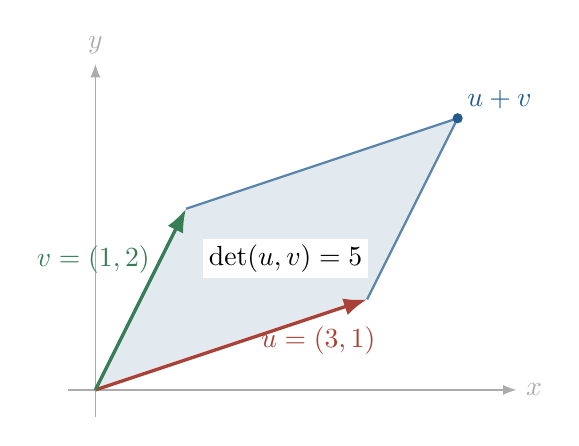
\begin{tikzpicture}[>=Latex,scale=1.15]
 \coordinate (O) at (0,0);
 \coordinate (U) at (3,1);
 \coordinate (V) at (1,2);
 \coordinate (UV) at (4,3);
 \fill[manifoldblue!13] (O)--(U)--(UV)--(V)--cycle;
 \draw[->,gray!65] (-0.3,0)--(4.65,0) node[right] {$x$};
 \draw[->,gray!65] (0,-0.3)--(0,3.6) node[above] {$y$};
 \draw[thick,manifoldblue!75] (U)--(UV)--(V);
 \draw[->,very thick,manifoldred] (O)--(U)
   node[pos=0.82,below] {$u=(3,1)$};
 \draw[->,very thick,manifoldgreen] (O)--(V)
   node[pos=0.72,left] {$v=(1,2)$};
 \fill[manifoldblue] (UV) circle (1.6pt) node[above right] {$u+v$};
 \node[fill=white,inner sep=2pt] at (2.1,1.45)
   {$\det(u,v)=5$};
\end{tikzpicture}
\caption{Iloczyn zewnętrzny w $\R^2$ koduje pole i orientację
równoległoboku. Zmiana kolejności wektorów zmienia znak.}
\label{fig:wedge-pole}
\end{figure}

\begin{twierdzenie}[Minory jako macierz $\Lambda^k A$]
\label{thm:minory-lambda}
Niech $A\colon\mathbb K^n\to\mathbb K^m$ ma macierz
$(a_{ij})$. W bazach uporządkowanych z
Twierdzenia~\ref{thm:wedge-baza} współczynnik macierzy
$\Lambda^k A$ w wierszu $I=(i_1<\cdots<i_k)$ i kolumnie
$J=(j_1<\cdots<j_k)$ jest wyznacznikiem podmacierzy
$A_{I,J}=(a_{i_a,j_b})_{a,b=1}^k$.
\end{twierdzenie}
\begin{proof}
Rozwijamy
$Ae_{j_1}\wedge\cdots\wedge Ae_{j_k}$ według
$Ae_{j_b}=\sum_i a_{i,j_b}e_i$. Przy bazowym
$e_{i_1}\wedge\cdots\wedge e_{i_k}$ pojawiają się tylko
składniki, których $k$ indeksów stanowi permutację $I$.
Po ustawieniu ich w kolejności rosnącej dostajemy
\[
 \sum_{\sigma\in S_k}\operatorname{sgn}(\sigma)
 \prod_{b=1}^k a_{i_{\sigma(b)},j_b}
 =\det A_{I,J}
\]
na mocy wzoru~\eqref{eq:det-leibniz} dla macierzy $k\times k$.
Nie występują żadne inne składniki przy wskazanym
wektorze bazowym, więc to jest szukany współczynnik.
\end{proof}

\begin{wniosek}[Wzór Cauchy'ego--Bineta]
\label{cor:cauchy-binet}
Dla macierzy $A$ o wymiarach $m\times n$ i $B$ o wymiarach
$n\times p$, oraz rosnących indeksów $I\subseteq\{1,\ldots,m\}$,
$J\subseteq\{1,\ldots,p\}$ długości $k$, gdzie $0\leq k\leq\min(m,p)$,
zachodzi
\begin{equation}\label{eq:cauchy-binet}
 \det\bigl((AB)_{I,J}\bigr)
 =\sum_{\substack{K\subseteq\{1,\ldots,n\}\\ |K|=k}}
 \det A_{I,K}\,\det B_{K,J}.
\end{equation}
\end{wniosek}
\begin{proof}
Z Twierdzenia~\ref{thm:potega-zewn-operatora} mamy
$\Lambda^k(AB)=(\Lambda^k A)(\Lambda^k B)$.
Twierdzenie~\ref{thm:minory-lambda} mówi, że macierze
trzech występujących tu operatorów mają za współczynniki
odpowiednie minory. Współczynnik iloczynu macierzy w
wierszu $I$ i kolumnie $J$ to suma po wszystkich
$k$-elementowych indeksach pośrednich $K$; jest ona
dokładnie prawą stroną~\eqref{eq:cauchy-binet}.
Dla $k=0$ obie strony są równe $1$. Gdy $k>n$,
nie ma indeksów $K$ i suma jest zerowa, zgodnie z tym,
że $\Lambda^k(\mathbb K^n)=0$.
\end{proof}

Oznaczamy przez $\operatorname{Alt}^k(V;\mathbb K)$ przestrzeń
alternujących $k$-liniowych funkcji $V^k\to\mathbb K$.
Dla $k=0$ jest to $\mathbb K$.

\begin{twierdzenie}[Kowektory zewnętrzne jako odwzorowania alternujące]
\label{thm:dual-zewnetrzny}
Dla skończenie wymiarowego $V$ istnieje kanoniczny izomorfizm
\[
 \mathcal E_k\colon\Lambda^k(V^*)
 \longrightarrow\operatorname{Alt}^k(V;\mathbb K),
\]
ustalony na iloczynach prostych przez
\begin{equation}\label{eq:wedge-form-det}
 \mathcal E_k(\alpha_1\wedge\cdots\wedge\alpha_k)
 (v_1,\ldots,v_k)
 =\det\bigl(\alpha_a(v_b)\bigr)_{a,b=1}^k.
\end{equation}
W szczególności $\Lambda^k(V^*)\cong(\Lambda^k V)^*$.
Dla kowektorów $\alpha,\beta$ otrzymujemy
\begin{equation}\label{eq:wedge-kowektory}
 \mathcal E_2(\alpha\wedge\beta)(u,v)
 =\alpha(u)\beta(v)-\alpha(v)\beta(u).
\end{equation}
Dla $k=0$ przyjmujemy $\mathcal E_0=\id_{\mathbb K}$ i wyznacznik
pustej macierzy równy $1$. Dla $k>\dim V$ obie strony izomorfizmu
są przestrzeniami zerowymi.
\end{twierdzenie}
\begin{proof}
Wyznacznik w~\eqref{eq:wedge-form-det} jest wieloliniowy
i alternujący w wierszach, a zatem w $\alpha_a$;
Twierdzenie~\ref{thm:wedge-multilinear}, zastosowane do $V^*$,
zapewnia dobrze określone odwzorowanie liniowe $\mathcal E_k$.
Jest ono alternujące w argumentach $v_b$, bo zamiana dwóch
kolumn wyznacznika zmienia znak, i wieloliniowe w tych
argumentach. Jeśli $e^1,\ldots,e^n$ jest bazą dualną,
to wartość $\mathcal E_k(e^{i_1}\wedge\cdots\wedge e^{i_k})$
na $(e_{j_1},\ldots,e_{j_k})$, dla indeksów rosnących,
wynosi $\delta_{I,J}$. Wektory bazowe w
$\Lambda^k(V^*)$ przechodzą więc na bazę dualną do
wektorów bazowych $\Lambda^k V$: daje to izomorfizm
$\Lambda^k(V^*)\cong(\Lambda^k V)^*$.
Każde odwzorowanie alternujące $V^k\to\mathbb K$ wyznacza
funkcjonał na $\Lambda^k V$ przez
Twierdzenie~\ref{thm:wedge-multilinear}, więc powyższy
izomorfizm obejmuje dokładnie wszystkie takie odwzorowania.
Przy $k=2$ wzór wyznacznika $2\times2$ daje
równość~\eqref{eq:wedge-kowektory}.
\end{proof}

\begin{uwaga}[Dwie zgodne normalizacje]
Utożsamienie $j_2$ z Twierdzenia~\ref{thm:wedge-alt} wysyła
$\alpha\wedge\beta$ na
$\tfrac12(\alpha\otimes\beta-\beta\otimes\alpha)$.
Natomiast $\mathcal E_2$ wysyła go na \emph{dwukrotność}
tego antysymetrycznego odwzorowania dwuliniowego: wzór
\eqref{eq:wedge-kowektory} nie zawiera czynnika $1/2$.
Ogólnie, po odczytaniu tensorów kowariantnych jako funkcji wieloliniowych,
zachodzi $\mathcal E_k=k!\,j_k$: suma w wyznaczniku ma te same
składniki ze znakami co antysymetryzacja, lecz bez dzielenia przez $k!$.
Po utożsamieniu elementów $\Lambda^k(V^*)$ z
odwzorowaniami alternującymi za pomocą $\mathcal E_k$, iloczyn
$\omega\wedge\eta$ stopni $k$ i $\ell$ jest dany przez
\begin{equation}\label{eq:wedge-alt-forms}
 (\omega\wedge\eta)(v_1,\ldots,v_{k+\ell})
 =\frac1{k!\ell!}\sum_{\sigma\in S_{k+\ell}}
 \operatorname{sgn}(\sigma)
 \omega(v_{\sigma(1)},\ldots,v_{\sigma(k)})
 \eta(v_{\sigma(k+1)},\ldots,v_{\sigma(k+\ell)}).
\end{equation}
Dla iloczynów kowektorów prostych jest to rozwinięcie
wyznacznika względem pierwszych $k$ wierszy: każdemu
wyborowi $k$ kolumn odpowiada $k!\ell!$ permutacji
wewnątrz dwóch bloków. Ponieważ takie iloczyny rozpinają
przestrzenie zewnętrzne, wzór zachodzi zawsze.
Równoważnie współczynnik przed
$\operatorname{Alt}_{k+\ell}(\omega\otimes\eta)$ jest równy
$(k+\ell)!/(k!\ell!)$, gdy $\omega,\eta$ są już funkcjami
alternującymi. Wynika to bezpośrednio z
$\mathcal E_m=m!j_m$ i wzoru na mnożenie dla $j_m$.
To wyjaśnia, dlaczego wzór w modelu tensorów antysymetrycznych
i wzór dla form mają różne współczynniki, mimo że opisują tę samą algebrę.
\end{uwaga}

\section{Tensory w punkcie rozmaitości}
\label{sec:tensory-rozmaitosc}

Dla gładkiej rozmaitości $M$ i $p\in M$ bierzemy teraz
$V=T_pM$ jako rzeczywistą przestrzeń liniową, a
$V^*=T_p^*M$ z Sekcji~\ref{sec:przestrzen-styczna}
i~\ref{sec:przestrzen-kostyczna}. Tensor typu $(r,s)$
\emph{w punkcie} $p$ jest elementem $T^r_s(T_pM)$;
to pojedynczy obiekt w jednym włóknie.

\begin{stwierdzenie}[Iloczyn tensorowy wiązek]
\label{prop:tensor-wiazek}
Niech $E,F\to M$ będą wiązkami wektorowymi rzędów
odpowiednio $a,b$. Przestrzenie $(E\otimes F)_p:=E_p\otimes F_p$
tworzą wiązkę wektorową rzędu $ab$ nad $M$. Jeśli
$g_{ji}$ i $h_{ji}$ są macierzami przejścia wiązek
$E$ i $F$, to macierzami przejścia $E\otimes F$
są $g_{ji}\otimes h_{ji}$.
\end{stwierdzenie}

\begin{proof}
Na obszarze, gdzie $E$ i $F$ mają bazy lokalne
$e_1,\ldots,e_a$ oraz $f_1,\ldots,f_b$, ich $ab$
iloczynów $e_u\otimes f_v$ stanowi bazę każdego włókna
$E_p\otimes F_p$ na mocy twierdzenia o bazie iloczynu
tensorowego. Gdy zmienimy obie bazy, wzór na współczynniki
iloczynu prostego pokazuje, że nowe współczynniki otrzymujemy
przez przemnożenie starych macierzą $g_{ji}\otimes h_{ji}$;
jej elementy są iloczynami gładkich funkcji. Na przecięciu
trzech obszarów własność złożenia z
Twierdzenia~\ref{thm:tensor-operatorow} daje
\[
 (g_{kj}\otimes h_{kj})(g_{ji}\otimes h_{ji})
   =(g_{kj}g_{ji})\otimes(h_{kj}h_{ji})
   =g_{ki}\otimes h_{ki}.
\]
Jest to warunek sklejania; macierze są odwracalne,
bo ich odwrotnościami są $g_{ji}^{-1}\otimes h_{ji}^{-1}$.
Konstrukcja wiązki z takich danych, podana w
Sekcji~\ref{sec:wiazki-wektorowe}, kończy dowód.
\end{proof}

\begin{definicja}[Pole tensorowe]
\index{pole tensorowe@Pole tensorowe}
\label{def:pole-tensorowe}
\emph{Pole tensorowe} typu $(r,s)$ przypisuje każdemu
$p\in M$ tensor $T_p\in T^r_s(T_pM)$ w sposób gładki.
Dokładnie: jest gładkim przekrojem wiązki
\begin{equation}\label{eq:wiazka-tensorowa}
 T^r_s M:=(TM)^{\otimes r}\otimes(T^*M)^{\otimes s}
 \longrightarrow M.
\end{equation}
Przy wykładniku $0$ rozumiemy czynnik jako wiązkę
trywialną $M\times\R$.
\end{definicja}

W lokalnej mapie $x^1,\ldots,x^n$ bazami włókien są
$\partial_i:=\partial/\partial x^i$ oraz dualne
$\dd x^j$, określone przez $\dd x^j(\partial_i)=\delta_i^j$.
Pole ma zatem postać
\begin{equation}\label{eq:pole-tensorowe-lokalnie}
 T=\sum_{\substack{i_1,\ldots,i_r\\j_1,\ldots,j_s}}
 T^{i_1\cdots i_r}{}_{j_1\cdots j_s}(x)
 \partial_{i_1}\otimes\cdots\otimes\partial_{i_r}
 \otimes\dd x^{j_1}\otimes\cdots\otimes\dd x^{j_s}.
\end{equation}
Warunek gładkości oznacza dokładnie, że wszystkie funkcje
$T^{i_1\cdots i_r}{}_{j_1\cdots j_s}(x)$ są gładkie.
W innej mapie bazowe wektory i kowektory się zmieniają;
przepisanie tej samej wartości $T_p$ w nowych bazach
narzuca współczynnikom prawa transformacji, które teraz rozpiszemy.
Niech $x$ i $y$ będą dwiema mapami wokół $p$, a
\[
 A^a{}_i=\frac{\partial y^a}{\partial x^i}(p),\qquad
 B^j{}_b=\frac{\partial x^j}{\partial y^b}(p),\qquad B=A^{-1}.
\]
Reguła łańcucha i dualność dają
\[
 \partial_{x^i}=\sum_a A^a{}_i\partial_{y^a},\qquad
 \dd x^j=\sum_b B^j{}_b\dd y^b.
\]
Podstawiając te równości w każdy czynnik
\eqref{eq:pole-tensorowe-lokalnie}, otrzymujemy
\begin{equation}\label{eq:tensor-zmiana-wspolrzednych}
 (T_y)^{a_1\cdots a_r}{}_{b_1\cdots b_s}
 =\sum_{I,J}
 \left(\prod_{\mu=1}^r A^{a_\mu}{}_{i_\mu}\right)
 \left(\prod_{\nu=1}^s B^{j_\nu}{}_{b_\nu}\right)
 (T_x)^{i_1\cdots i_r}{}_{j_1\cdots j_s}.
\end{equation}
Wszystkie wartości odnoszą się do tego samego punktu $p$;
zmienia się jedynie jego opis i baza. Każdy górny indeks wnosi
macierz Jacobiego $A$, a każdy dolny jej odwrotność $B$.
Odwracając zamianę map, odzyskujemy stare współczynniki.
Ponieważ $A,B$ są gładkie, gładkość współczynników w jednej
mapie pociąga ją w każdej innej.

Wiązka~\eqref{eq:wiazka-tensorowa} powstaje
przez wielokrotne zastosowanie
Stwierdzenia~\ref{prop:tensor-wiazek} do $TM$ i $T^*M$.

Typ $(0,0)$ to zwykła funkcja gładka, typ $(1,0)$ to
pole wektorowe z Rozdziału~\ref{ch:pola}, a typ $(0,2)$
to gładko zmieniająca się rodzina form dwuliniowych
na przestrzeniach stycznych. Iloczyn tensorowy i kontrakcja
działają \emph{punkt po punkcie}. Pozostawiają pola gładkie,
bo w mapach ich współczynniki są sumami iloczynów
gładkich funkcji współczynnikowych.

\begin{przyklad}[Tensor identycznościowy]
Operator $\id_{T_pM}$ z~\eqref{eq:endo-tensor} odpowiada
w dowolnej bazie $e_i$ tensorowi
\[
 \mathsf I_p=\sum_i e_i\otimes e^i\in T^1_1(T_pM).
\]
Jego zapis w mapie to $\sum_i\partial_i\otimes\dd x^i$.
Nie zależy od mapy: po przyłożeniu do dowolnego $v$
odzyskujemy $\sum_i e^i(v)e_i=v$, a izomorfizm
$T^1_1(T_pM)\cong\operatorname{End}(T_pM)$ jest
iniektywny. Tensor $\mathsf I$ jest zatem globalnym
gładkim polem tensorowym, mimo że zapisaliśmy go lokalnie.
\end{przyklad}

\begin{przyklad}[Tensor jako iloczyn skalarny]
Na $\R^2$ pole
$g=\dd x\otimes\dd x+\dd y\otimes\dd y$
przypisuje każdemu punktowi ten sam iloczyn skalarny.
Dla $u=a\partial_x+b\partial_y$ i
$v=c\partial_x+d\partial_y$ mamy
$g(u,v)=ac+bd$. Oznacza to, że tensor typu $(0,2)$
można czytać jako przepis przyjmujący \emph{dwa}
wektory styczne w jednym punkcie i zwracający liczbę.
Sama lista jego współczynników zmieni się przy zamianie
współrzędnych, ale wartość $g(u,v)$ pozostanie ta sama.
Na jednowymiarowym przykładzie widać konkretny czynnik:
dla $x>0$ i $y=x^2$ tensor $\dd x\otimes\dd x$ ma zapis
$\frac1{4y}\dd y\otimes\dd y$, bo
$\dd x=\frac1{2\sqrt y}\dd y$. Zmiana współrzędnych nie
pozwala więc po prostu zastąpić symbolu $x$ symbolem $y$
przy pozostawieniu tych samych współczynników.
\end{przyklad}

Podobnie $\Lambda^k(T_pM)$ ma wymiar $\binom nk$.
W przypadku różniczki $\dd F_p\colon T_pM\to T_{F(p)}N$
między rozmaitościami tego samego wymiaru,
$\Lambda^n(\dd F_p)$ działa między ich jednowymiarowymi
potęgami zewnętrznymi. Jest niezerowe dokładnie wtedy,
gdy $\dd F_p$ jest izomorfizmem: wynika to z dowodu
Twierdzenia~\ref{thm:det-wlasnosci}, zastosowanego do baz
w dwóch różnych przestrzeniach. W mapach odpowiada temu
warunek niezerowego wyznacznika macierzy Jacobiego.
W odróżnieniu od endomorfizmu jednej przestrzeni, dla mapy
$T_pM\to T_{F(p)}N$ nie otrzymujemy jednak kanonicznego skalara
„wyznacznik” bez wyboru baz lub elementów objętości w obu włóknach.
Kanoniczne jest odwzorowanie $\Lambda^n(\dd F_p)$ między
dwiema prostymi; jego macierz liczbową określają wybrane mapy.

\begin{uwaga}[Cztery sposoby widzenia tej samej konstrukcji]
Iloczyn tensorowy powstaje z dwuliniowości
(Definicja~\ref{def:tensor-universal}); algebra tensorowa
gromadzi wszystkie stopnie i mnoży przez konkatenację
(Definicja~\ref{def:algebra-tensorowa}). Symetryzator
$\operatorname{Sym}_k$ wybiera część niezmienniczą względem
permutacji, zaś $\operatorname{Alt}_k$ część zmieniającą znak.
Algebra zewnętrzna jest ilorazem, w którym kwadrat każdego
wektora znika (Definicja~\ref{def:algebra-zewnetrzna}).
Twierdzenie~\ref{thm:wedge-alt} mówi dokładnie, jak przejść
od tego ilorazu do tensorów antysymetrycznych.
\end{uwaga}

\section{Różniczkowanie pól tensorowych: pochodna Liego}
\label{sec:lie-tensory}

Pole tensorowe ma wartości w różnych przestrzeniach nad
różnymi punktami. Dlatego wyrażenie ,,odejmij $T_q-T_p$''
nie ma sensu, dopóki nie wskażemy sposobu przeniesienia
obu tensorów do jednego włókna. W Sekcji~\ref{sec:liego}
przepływ pola $X$ zrobił to dla pól wektorowych;
ta sama konstrukcja działa na każdym typie tensora.

Samo różniczkowanie współczynników w mapie nie rozwiązuje
problemu: ich pochodne zmieniają się przy zmianie współrzędnych.
Na przykład na $(0,\infty)$ wektor $Y=\partial_x$ ma w
mapie $x$ stały współczynnik $Y^x=1$, więc
$\partial_xY^x=0$. Po podstawieniu $y=x^2$ mamy
$Y=2\sqrt y\,\partial_y$ i
$\partial_yY^y=1/\sqrt y\ne0$.
Różnica pochodzi od zmiany samej bazy $\partial_y$.
Pochodna Liego uwzględnia również tę zmianę.

\begin{definicja}[Cofnięcie pola tensorowego]
\index{cofniecie pola tensorowego@Cofnięcie pola tensorowego}
\label{def:cofniecie-tensora}
Niech $F\colon U\to V$ będzie dyfeomorfizmem między
otwartymi podzbiorami $M$. Dla pola wektorowego $Y$ i
pola kowektorowego $\alpha$ na $V$ definiujemy w $p\in U$
\begin{align*}
 (F^*Y)_p&:=(\dd F_p)^{-1}Y_{F(p)}\in T_pM,\\
 (F^*\alpha)_p(v)&:=\alpha_{F(p)}(\dd F_pv),
 \qquad v\in T_pM.
\end{align*}
Dla funkcji kładziemy $F^*f=f\circ F$.
Na tensorach prostych cofamy każdy czynnik osobno,
np.\ $F^*(Y\otimes\alpha)=F^*Y\otimes F^*\alpha$,
i przedłużamy liniowo na sumy w każdym włóknie. Do gładkości
wystarczy lokalne rozwinięcie w bazie tensorowej; nie zakładamy
istnienia jednej globalnej bazy ani globalnego rozkładu na tensory proste.
Dostajemy pole
tego samego typu na $U$. W szczególności
$F^*(fT)=(f\circ F)F^*T$, a nie $fF^*T$.
Współczynniki są gładkie: różniczka i jej macierz odwrotna
zależą gładko od punktu, a działania tensorowe są wieloliniowe.
\end{definicja}

Przy cofaniu wektora używamy odwrotnej różniczki,
a przy cofaniu kowektora różniczki bez odwracania:
obie wartości muszą ostatecznie należeć do włókna nad $p$.
Wzór dla tensorów prostych jest dobrze określony na
iloczynach tensorowych, ponieważ każda z operacji na
czynnikach jest liniowa. W szczególności cofnięcie zachowuje
iloczyn tensorowy i kontrakcję. To drugie można sprawdzić
na jednej parze:
\[
 (F^*\alpha)_p\bigl((F^*Y)_p\bigr)
 =\alpha_{F(p)}\bigl(\dd F_p(\dd F_p)^{-1}Y_{F(p)}\bigr)
 =\alpha_{F(p)}(Y_{F(p)}).
\]
Obie strony są cofnięciem funkcji $p\mapsto\alpha_p(Y_p)$;
z liniowości wynikają analogiczne równości dla innych tensorów.

\begin{definicja}[Pochodna Liego dowolnego pola tensorowego]
\index{pochodna liego dowolnego pola tensorowego@Pochodna Liego dowolnego pola tensorowego}
\label{def:lie-tensor}
Niech $\Phi_t=\Phi_t^X$ oznacza lokalny przepływ pola $X$.
Dla pola tensorowego $T$ dowolnego typu kładziemy
\begin{equation}\label{eq:lie-tensor-def}
 (\Lie_XT)_p
 :=\left.\frac{\dd}{\dd t}\right|_{t=0}
 (\Phi_t^*T)_p.
\end{equation}
Każdy tensor $(\Phi_t^*T)_p$ należy do tej samej
przestrzeni $T^r_s(T_pM)$, zatem pochodna jest
zwykłą pochodną krzywej w przestrzeni liniowej. Jest to gładkie
pole tensorowe: w każdej mapie współczynniki cofnięcia są gładkie
łącznie w $(t,p)$, więc ich pochodne po $t$ w zerze są gładkie w $p$.
\end{definicja}

W stopniu $(0,0)$ wzór~\eqref{eq:lie-tensor-def} daje
$\Lie_Xf=X(f)$, ponieważ $\Phi_t^*f=f\circ\Phi_t$.
Dla typu $(1,0)$ odzyskujemy dokładnie
$\Lie_XY=[X,Y]$ z Twierdzenia~\ref{thm:lie-nawias}.
Dowód tamtego twierdzenia wyjaśnia szczegółowo znak:
przenosimy $Y_{\Phi_t(p)}$ z powrotem różniczką
przepływu $\Phi_{-t}$.

\begin{twierdzenie}[Reguła Leibniza i zgodność z kontrakcją]
\label{thm:lie-tensor-reguly}
Dla pól tensorowych $S,T$, funkcji $f$, pola wektorowego
$Y$ i pola kowektorowego $\alpha$ mamy
\begin{align}
 \Lie_X(S\otimes T)
 &= (\Lie_XS)\otimes T+S\otimes(\Lie_XT),
 \label{eq:lie-tensor-leibniz}\\
 \Lie_X(fT)&=X(f)T+f\Lie_XT,
 \label{eq:lie-tensor-funkcja}\\
 (\Lie_X\alpha)(Y)
 &=X\bigl(\alpha(Y)\bigr)-\alpha([X,Y]),
 \label{eq:lie-kowektor}\\
 \Lie_X(C(S))&=C(\Lie_XS),
 \label{eq:lie-kontrakcja}
\end{align}
gdzie w ostatnim wzorze $C$ jest dowolną kontrakcją
jednego indeksu wektorowego z jednym kowektorowym.
\end{twierdzenie}
\begin{proof}
Ustalmy punkt $p$. Cofnięcie zachowuje iloczyn tensorowy:
$\Phi_t^*(S\otimes T)=\Phi_t^*S\otimes\Phi_t^*T$.
Obie krzywe tensorów po prawej stronie leżą w stałych
przestrzeniach nad $p$; różniczkując ich iloczyn
dwuliniowy w $t=0$ dostajemy
\eqref{eq:lie-tensor-leibniz}. Traktując $f$ jako tensor
typu $(0,0)$, otrzymujemy
\eqref{eq:lie-tensor-funkcja} z $\Lie_Xf=X(f)$.

Dla kowektora i wektora równanie o zachowaniu ewaluacji,
wykazane tuż przed definicją, przyjmuje postać
\[
 \Phi_t^*\bigl(\alpha(Y)\bigr)
 =(\Phi_t^*\alpha)(\Phi_t^*Y).
\]
Lewa strona po zróżniczkowaniu w zerze wynosi
$X(\alpha(Y))$. Prawa, przez zwykłą regułę
różniczkowania wartości kowektora na wektorze,
wynosi $(\Lie_X\alpha)(Y)+\alpha(\Lie_XY)$.
Z~$\Lie_XY=[X,Y]$ otrzymujemy
\eqref{eq:lie-kowektor}.

Wreszcie, cofnięcie i kontrakcja spełniają
$\Phi_t^*C(S)=C(\Phi_t^*S)$, co dla pojedynczej
pary sprawdziliśmy powyżej. Kontrakcja jest liniowym
odwzorowaniem między przestrzeniami tensorów w $p$, więc
można ją przenieść przez pochodną po $t$.
To daje~\eqref{eq:lie-kontrakcja}.
\end{proof}

\begin{twierdzenie}[Wzór we współrzędnych]
\label{thm:lie-tensor-wspolrzedne}
Niech $X=\sum_{a=1}^nX^a\partial_a$ i niech $T$ ma
współczynniki $T^I{}_J$ z~\eqref{eq:pole-tensorowe-lokalnie},
gdzie $I=(i_1,\ldots,i_r)$ i $J=(j_1,\ldots,j_s)$.
Symbol $I_{\mu\leftarrow a}$ oznacza zastąpienie w $I$
indeksu $i_\mu$ przez $a$, a $J_{\nu\leftarrow a}$
oznacza to samo w $J$. Wtedy
\begin{equation}\label{eq:lie-tensor-komponenty}
\begin{aligned}
 (\Lie_XT)^I{}_J
 &=\sum_{a=1}^nX^a\partial_a T^I{}_J
 -\sum_{\mu=1}^r\sum_{a=1}^n
   (\partial_aX^{i_\mu})T^{I_{\mu\leftarrow a}}{}_J\\
 &\quad+\sum_{\nu=1}^s\sum_{a=1}^n
   (\partial_{j_\nu}X^a)T^I{}_{J_{\nu\leftarrow a}}.
\end{aligned}
\end{equation}
Pierwszy wyraz różniczkuje funkcje współczynnikowe,
każdy indeks wektorowy wnosi wyraz z minusem,
a każdy indeks kowektorowy wyraz z plusem.
Na przykład dla pola operatorów $S\in\Gamma(T^1_1M)$
wzór ten ma łatwą do odczytania postać
\[
 (\Lie_XS)^i{}_j
 =\sum_a X^a\partial_aS^i{}_j
  -\sum_a S^a{}_j\partial_aX^i
  +\sum_a S^i{}_a\partial_jX^a.
\]
\end{twierdzenie}
\begin{proof}
Z~\eqref{eq:nawias-wspolrzedne}, zastosowanego do
$Y=\partial_i$, wynika
\[
 \Lie_X\partial_i=[X,\partial_i]
 =-\sum_a(\partial_iX^a)\partial_a,
\]
ponieważ współczynniki pola $\partial_i$ są stałe.
Z kolei $\dd x^j(\partial_i)=\delta_i^j$ jest funkcją
stałą. Wstawiając $Y=\partial_i$ i $\alpha=\dd x^j$
do~\eqref{eq:lie-kowektor}, dostajemy
\[
 (\Lie_X\dd x^j)(\partial_i)
 =X(\delta_i^j)-\dd x^j([X,\partial_i])
 =\partial_iX^j.
\]
Wektory $\partial_i$ tworzą bazę, zatem
$\Lie_X\dd x^j=\sum_i(\partial_iX^j)\dd x^i$.
Teraz rozwińmy $T$ według~\eqref{eq:pole-tensorowe-lokalnie}
i stosujmy~\eqref{eq:lie-tensor-leibniz} kolejno
do funkcji współczynnikowej oraz do każdego czynnika.
Różniczkowanie funkcji daje pierwszy wyraz
\eqref{eq:lie-tensor-komponenty}. Dla ustalonego miejsca
wektorowego $\mu$ współczynnik przy bazowym
$\partial_{i_\mu}$ po zróżniczkowaniu wcześniejszego
czynnika $\partial_a$ wynosi
$-\sum_a(\partial_aX^{i_\mu})T^{I_{\mu\leftarrow a}}{}_J$;
sumowanie po $\mu$ daje drugi wyraz wzoru.
Dla ustalonego miejsca kowektorowego $\nu$ wcześniejszy
czynnik $\dd x^a$ wnosi do współczynnika przy
$\dd x^{j_\nu}$ sumę
$\sum_a(\partial_{j_\nu}X^a)T^I{}_{J_{\nu\leftarrow a}}$;
po zsumowaniu po $\nu$ otrzymujemy trzeci wyraz.
Ponieważ tensory bazowe są liniowo niezależne,
ich współczynniki są dokładnie podanymi wyrażeniami.
\end{proof}

\begin{przyklad}[Sprawdzenie znaków na przepływie]
Na $\R^2$ weźmy $X=x\partial_x$. Jego przepływ to
$\Phi_t(x,y)=(e^tx,y)$, więc
\[
 \Phi_t^*\partial_x=e^{-t}\partial_x,
 \qquad \Phi_t^*\dd x=e^t\dd x.
\]
Po zróżniczkowaniu w zerze otrzymujemy
$\Lie_X\partial_x=-\partial_x=[X,\partial_x]$
oraz $\Lie_X\dd x=\dd x$. Pierwszy znak jest ujemny,
bo cofamy wektor różniczką odwrotnego przepływu;
drugi dodatni, bo kowektor działa na różniczce przepływu.
Wyniki są zgodne z tym, że $\dd x(\partial_x)=1$
pozostaje funkcją stałą: $1+(-1)=0$ w regule
Leibniza dla ewaluacji.
\end{przyklad}

\begin{przyklad}[Jak zmienia się tensor metryczny]
Dla $g=\dd x\otimes\dd x+\dd y\otimes\dd y$ i
$X=x\partial_x$ mamy
\[
 \Phi_t^*g=e^{2t}\dd x\otimes\dd x
             +\dd y\otimes\dd y,\qquad
 \Lie_Xg=2\dd x\otimes\dd x.
\]
Przepływ rozciąga kierunek $x$; gdy tensor mierzy
iloczyny skalarne dwóch wektorów, pojawia się czynnik
$e^t$ dla każdego z dwóch kowektorowych miejsc.
\end{przyklad}

\begin{uwaga}[Jaką pochodną zdefiniowaliśmy?]
Pochodna Liego porównuje tensory za pomocą przepływu
\emph{konkretnego} pola $X$. Jej wzór wymaga tylko struktury
gładkiej i pola $X$. Jeśli chcielibyśmy porównywać tensory
wzdłuż dowolnej krzywej bez wskazanego przepływu,
potrzebowalibyśmy dodatkowej reguły przenoszenia między
przestrzeniami stycznymi, nazywanej \emph{koneksją} (połączeniem).
Na przykład $\Lie_{x\partial_x}\partial_x=-\partial_x$
chociaż współczynniki pola $\partial_x$ są stałe:
wynik uwzględnia ruch bazy pod przepływem.
\end{uwaga}

\par\smallskip
{\footnotesize\noindent\emph{Dalsza lektura:}
\href{https://math.stanford.edu/~conrad/diffgeomPage/handouts/tensor.pdf}
{B. Conrad, \emph{Tensor algebras, tensor pairings, and duality}},
notatki do Math 396, s. 1--13: własności uniwersalne i dualność;
\href{https://doi.org/10.1007/978-1-4419-9982-5}
{J. M. Lee, \emph{Introduction to Smooth Manifolds}, wyd. 2},
rozdziały 12 i 14: pola tensorowe, formy alternujące
i pochodne Liego.\par}
\clearpage

\chapter{Grassmanniany, algebra Clifforda i spinory}
\label{ch:grass-spin}
\index{grupa spin@Grupa Spin}

W Rozdziale~\ref{ch:algebra-tensorowa} skonstruowaliśmy iloczyn
zewnętrzny i wiązki tensorowe. Teraz zadamy trzy kolejne pytania:
jak opisać \emph{przestrzeń wszystkich podprzestrzeni} danego wymiaru,
jak zmienić algebrę zewnętrzną, aby uwzględniała iloczyn skalarny,
i dlaczego obrót o $2\pi$ może zmieniać znak spinora.
Odpowiedzi prowadzą kolejno do grassmannianów, algebr Clifforda
i grup Spin. Przykłady w wymiarach $2$ i $3$ pozwolą nam
sprawdzać każdą konwencję znaku na konkretnych macierzach.

\section{Grassmannian jako przestrzeń podprzestrzeni}
\label{sec:grass-atlas}

Przez $\mathbb K$ oznaczamy w tej sekcji $\R$ albo $\C$.
Jeśli $0\leq k\leq n$, \emph{grassmannian}
$\operatorname{Gr}_k(\mathbb K^n)$ to zbiór wszystkich
$k$-wymiarowych podprzestrzeni liniowych $\mathbb K^n$.
Jego \emph{punktem} jest cała podprzestrzeń $L$,
a nie wektor w $L$. Na przykład
$\operatorname{Gr}_1(\R^n)=\mathbb{RP}^{n-1}$
z Przykładu~\ref{prz:RPn}, a
$\operatorname{Gr}_1(\C^n)=\mathbb{CP}^{n-1}$.
Dla $k=0$ i $k=n$ grassmannian jest jednym punktem.
Dla dowolnej $n$-wymiarowej przestrzeni $V$ nad $\mathbb K$
piszemy analogicznie $\operatorname{Gr}_k(V)$; wybór bazy
identyfikuje go z powyższym modelem, lecz konstrukcje nie zależą od tej bazy.

\begin{twierdzenie}[Mapy wykresowe grassmannianu]
\label{thm:grass-atlas}
Niech $\mathbb K^n=P\oplus Q$, gdzie $\dim_{\mathbb K}P=k$.
Zbiór
\[
 U_P=\{L\in\operatorname{Gr}_k(\mathbb K^n):
           \pi_P|_L:L\longrightarrow P\text{ jest izomorfizmem}\}
\]
można jednoznacznie opisać odwzorowaniami liniowymi
$A:P\to Q$: punktowi $A$ odpowiada jego
\emph{wykres} $\Gamma(A)=\{u+Au:u\in P\}$.
Mapy $\Gamma(A)\mapsto A$ tworzą gładki atlas
grassmannianu. Jego wymiar nad $\mathbb K$ wynosi
$k(n-k)$. W przypadku zespolonym atlas jest holomorficzny,
a rzeczywisty wymiar wynosi $2k(n-k)$.
Oznaczenie $U_P$ zależy również od wybranego dopełnienia $Q$;
pomijamy je w indeksie tylko dla skrócenia zapisu.
\end{twierdzenie}
\begin{proof}
Jeśli $L=\Gamma(A)$, to $\pi_P(u+Au)=u$, więc
$\pi_P|_L$ jest izomorfizmem. W drugą stronę, dla
$L\in U_P$ określmy
\[
 A_L:=\pi_Q|_L\circ(\pi_P|_L)^{-1}:P\longrightarrow Q.
\]
Każdy $v\in L$ ma postać $u+\pi_Qv=u+A_Lu$
dla $u=\pi_Pv$. Stąd $L=\Gamma(A_L)$; dowiedliśmy
zarówno istnienia, jak i jednoznaczności parametru.

Sprawdźmy przejścia między mapami, a nie tylko ich
liczbę. Niech $\mathbb K^n=P'\oplus Q'$ będzie drugim
rozkładem. Dla $A:P\to Q$ połóżmy
$T_A:P\to\mathbb K^n$, $T_A(u)=u+Au$.
Wykres $\Gamma(A)$ należy do $U_{P'}$ dokładnie wtedy,
gdy $D_A:=\pi_{P'}T_A:P\to P'$ jest odwracalny.
Po wybraniu baz $P,P'$ wyznacznik macierzy $D_A$ zależy
wielomianowo od współczynników $A$;
warunek $\det D_A\ne0$ jest więc otwarty. W nowej mapie
parametr ma postać
\begin{equation}\label{eq:grass-przejscie}
 A'=\pi_{Q'}T_A\circ(\pi_{P'}T_A)^{-1}:P'\longrightarrow Q'.
\end{equation}
Odwracanie macierzy jest gładkie na zbiorze macierzy
odwracalnych, a nad $\C$ jest tam także holomorficzne
(wzór przez dopełnienia algebraiczne i wyznacznik).
Każde $L$ leży w $U_L$, bo dla rozkładu
$\mathbb K^n=L\oplus Q$ otrzymujemy $A_L=0$.
Atlasy pokrywają zatem cały zbiór. Współczynniki
$A\in\operatorname{Hom}_{\mathbb K}(P,Q)$ tworzą
przestrzeń $\mathbb K^{(n-k)k}$, co daje wymiar.

Definiujemy topologię przez atlas: zbiór jest otwarty, gdy
jego obraz w każdej z map wykresowych jest otwarty.
Otwartość dziedzin przejść i ich ciągłość zapewniają, że
same $U_P$ są otwarte, a mapy są homeomorfizmami.
Uzasadnijmy również pozostałe własności topologiczne.
Wybierzmy standardowy iloczyn skalarny, a nad $\C$ hermitowski;
gwiazdka oznacza operator sprzężony. W tym kroku
ograniczmy się do rozkładów ortogonalnych $Q=P^\perp$;
takie mapy wciąż pokrywają cały grassmannian
(dla danego $L$ bierzemy $P=L$).
Wzór~\eqref{eq:grass-przejscie} zapewnia zgodność
z pozostałymi mapami. Każdemu $L$
przypiszmy macierz rzutowania ortogonalnego $\Pi_L$.
Jest ona wyznaczona jednoznacznie przez $L$, a jej
współczynniki w mapie wykresowej są gładkie:
\[
 \Pi_{\Gamma(A)}
  =T_A(T_A^*T_A)^{-1}T_A^*.
\]
Odwrót na $U_P$ jest również ciągły w macierzach
rzutowania, ponieważ dla $L\in U_P$
\[
 A_L=\pi_Q\Pi_L|_P\,(\pi_P\Pi_L|_P)^{-1}.
\]
Ostatnia odwrotność istnieje, gdyż przy ortogonalnym
rzutowaniu $\pi_P$ odwzorowanie $\Pi_L|_P:P\to L$
jest sprzężeniem izomorfizmu
$\pi_P|_L:L\to P$. Nasza topologia zgadza się więc
z topologią podzbioru macierzy rzutowania: $U_P$ jest w tym
modelu zbiorem, gdzie $\pi_P\Pi_L|_P$ jest odwracalne,
a więc zbiorem otwartym. Oba podane wzory są ciągłe na tych mapach.
Zbiór $\Pi^*=\Pi$, $\Pi^2=\Pi$, $\operatorname{tr}\Pi=k$
jest domknięty i ograniczony w skończenie wymiarowej
przestrzeni macierzy, a więc zwarty. Istotnie, samosprzężone
idempotenty mają wartości własne $0,1$, więc norma operatorowa
jest co najwyżej $1$, a ślad jest rangą. Są zatem dokładnie
rzutami na $k$-płaszczyzny. Ten model jest także
Hausdorffa i ma przeliczalną bazę. Atlas definiuje
zatem rozmaitość w sensie Rozdziału~\ref{ch:rozmaitosci}.
\end{proof}

\begin{figure}[!htbp]
\centering
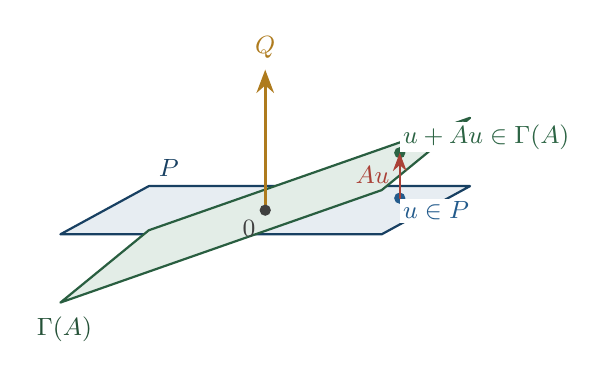
\begin{tikzpicture}[>=Stealth,line cap=round,line join=round,scale=1.02]
 \filldraw[fill=manifoldblue!11,draw=manifoldblue!70!black,thick]
 (-2.55,-.3)--(1.45,-.3)--(2.55,.3)--(-1.45,.3)--cycle;
 \filldraw[fill=manifoldgreen!14,draw=manifoldgreen!75!black,thick]
 (-2.55,-1.15)--(1.45,.25)--(2.55,1.15)--(-1.45,-.25)--cycle;
 \draw[->,manifoldgold!85!black,very thick] (0,0)--(0,1.75)
  node[above,font=\small] {$Q$};
 \fill[black!75] (0,0) circle (2pt) node[below left,font=\small] {$0$};
 \fill[manifoldblue] (1.675,.15) circle (2pt)
  node[below right,fill=white,inner sep=1pt,font=\small] {$u\in P$};
 \fill[manifoldgreen!80!black] (1.675,.715) circle (2pt)
  node[above right,fill=white,inner sep=1pt,font=\small] {$u+Au\in\Gamma(A)$};
 \draw[->,manifoldred,thick] (1.675,.15)--(1.675,.715)
  node[midway,left,font=\small] {$Au$};
 \node[manifoldblue!70!black,font=\small\bfseries] at (-1.2,.52) {$P$};
 \node[manifoldgreen!65!black,font=\small\bfseries] at (-2.5,-1.48) {$\Gamma(A)$};
\end{tikzpicture}
\caption{Mapa wykresowa grassmannianu. Przestrzeń $P$ jest
punktem odniesienia; pobliska płaszczyzna $\Gamma(A)$ powstaje,
gdy nad $u\in P$ odkładamy przemieszczenie $Au\in Q$.}
\label{fig:grass-wykres}
\end{figure}

\begin{przyklad}[Mała mapa, a nie cały grassmannian]
Na $\operatorname{Gr}_1(\R^2)=\mathbb{RP}^1$ ustalmy
$P=\R e_1$ i $Q=\R e_2$. Prosta
$L_a=\operatorname{span}(e_1+ae_2)$ ma współrzędną
$a\in\R$. Brakuje dokładnie jednej prostej, $\R e_2$:
rzutowanie na $P$ jest na niej zerowe. Zatem mapa
wykresowa jest lokalna, podobnie jak mapa stereograficzna
nie pokrywa całej sfery.
\end{przyklad}

\section{Przestrzeń styczna i wiązka tautologiczna}
\label{sec:grass-styczna}

Wektor styczny do grassmannianu opisuje \emph{pierwszy
rząd zmiany podprzestrzeni}. Wektory należące już do
danej podprzestrzeni nie zmieniają jej położenia:
istotna jest część wychodząca poza nią.

\begin{twierdzenie}[Styczne jako odwzorowania do ilorazu]
\label{thm:grass-styczna}
Dla $L\in\operatorname{Gr}_k(V)$ istnieje kanoniczny
izomorfizm
\begin{equation}\label{eq:grass-styczna}
 T_L\operatorname{Gr}_k(V)
  \cong\operatorname{Hom}_{\mathbb K}(L,V/L).
\end{equation}
Nad $\C$ prawa strona jest zespoloną przestrzenią
styczną; jej podłożem rzeczywistym jest rzeczywista
przestrzeń styczna.
\end{twierdzenie}
\begin{proof}
Niech $L(t)$ będzie gładką krzywą podprzestrzeni,
$L(0)=L$. Dla $v\in L$ wybierzmy gładką krzywą
$v(t)\in L(t)$ z $v(0)=v$. Definiujemy
$D_{L'(0)}(v):=[v'(0)]\in V/L$, gdzie nawias oznacza
klasę modulo $L$. Pokażmy niezależność od wyboru
$v(t)$. Różnica dwóch takich krzywych $w(t)\in L(t)$
ma $w(0)=0$. W gładkiej lokalnej bazie $s_i(t)$
zapisuje się $w(t)=\sum_i a_i(t)s_i(t)$ z
$a_i(0)=0$, zatem
$w'(0)=\sum_i a_i'(0)s_i(0)\in L$. Klasa
$[v'(0)]$ nie zmienia się. Zmiana parametryzacji
krzywej nie jest jedyną możliwą zmianą przedstawiciela wektora
stycznego; niezależność od dowolnej krzywej o tym samym wektorze
stycznym sprawdzimy teraz w mapie.

Ustalmy teraz uzupełnienie $V=L\oplus Q$.
W mapie z Twierdzenia~\ref{thm:grass-atlas} mamy
$L(t)=\Gamma(A(t))$ i $A(0)=0$.
Wybieramy $v(t)=v+A(t)v$. Wtedy
\[
 D_{L'(0)}(v)=[A'(0)v]\in V/L.
\]
Tak samo $s_i(t)=e_i+A(t)e_i$ dla bazy $(e_i)$ przestrzeni $L$
daje gładką bazę używaną powyżej. Wzór zależy tylko od $A'(0)$,
czyli współrzędnych wektora stycznego, a nie od dalszego przebiegu krzywej.
Jeśli $D_{L'(0)}=0$, to $A'(0)v\in Q\cap L=0$ dla każdego $v$,
więc $A'(0)=0$ i wektor styczny jest zerowy. To dowodzi iniektywności.
Utożsamienie $Q\cong V/L$ pokazuje, że
$D_{L'(0)}$ jest liniowe w $v$. Każdy
$D\in\operatorname{Hom}(L,V/L)$ można otrzymać:
wybierzmy odpowiadające mu odwzorowanie $A:L\to Q$
i krzywą $L(t)=\Gamma(tA)$. Jej pochodna daje
właśnie $D$. Konstrukcja rozpoczęła się od
krzywej i klas modulo $L$, więc otrzymany
izomorfizm nie zależy od wybranego $Q$.
\end{proof}

\begin{definicja}[Wiązka tautologiczna]
\index{wiazka tautologiczna@Wiązka tautologiczna}
\label{def:grass-taut}
Nad $\operatorname{Gr}_k(V)$ określamy
\emph{wiązkę tautologiczną}
\[
 \gamma^k
 :=\{(L,v)\in\operatorname{Gr}_k(V)\times V:v\in L\}
 \longrightarrow\operatorname{Gr}_k(V),\qquad (L,v)\mapsto L.
\]
Jej włókno w punkcie $L$ jest dosłownie podprzestrzenią
$L\subseteq V$.
\end{definicja}

\begin{stwierdzenie}[Lokalność i wiązka ilorazowa]
\label{prop:grass-wiazki}
Wiązka $\gamma^k$ ma rząd $k$. Jest podwiązką
wiązki trywialnej $\operatorname{Gr}_k(V)\times V$.
Istnieje też wiązka ilorazowa $\mathcal Q$ z
włóknem $\mathcal Q_L=V/L$, rzędu $n-k$,
oraz kanoniczny dokładny ciąg wiązek
\begin{equation}\label{eq:grass-ciag}
 0\longrightarrow\gamma^k
 \longrightarrow\operatorname{Gr}_k(V)\times V
 \longrightarrow\mathcal Q\longrightarrow0.
\end{equation}
Po wybraniu iloczynu skalarnego otrzymujemy
$\mathcal Q\cong(\gamma^k)^\perp$.
\end{stwierdzenie}
\begin{proof}
Na $U_P$ każdy element $L=\Gamma(A)$ zawiera
dokładnie jeden wektor $u+Au$ dla danego $u\in P$.
Odwzorowanie $(L,u)\mapsto(L,u+Au)$ jest zatem lokalną
trywializacją $U_P\times P\cong\gamma^k|_{U_P}$;
jej odwrotność to $(L,v)\mapsto(L,\pi_Pv)$.
Oba odwzorowania są gładkie, a na włóknach liniowe.
W tym samym rozkładzie $V=P\oplus Q$ klasa
$[w]\in V/\Gamma(A)$ ma jednoznacznego
reprezentanta w $Q$: od $w$ odejmujemy
$u+Au\in\Gamma(A)$, gdzie $u=\pi_Pw$.
Stąd lokalnie $\mathcal Q|_{U_P}\cong U_P\times Q$.
Na każdym włóknie włączenie $L\hookrightarrow V$
jest iniekcją, a naturalne odwzorowanie $V\to V/L$ jest
surjekcją z jądrem $L$, co wyjaśnia \emph{dokładność}
ciągu~\eqref{eq:grass-ciag}. Iloczyn skalarny
identyfikuje klasę $[v]$ z $(\id-\Pi_L)v\in L^\perp$.
Rzut zależy gładko od $L$, więc jest to izomorfizm wiązek,
a nie tylko rodzina izomorfizmów włókien.
\end{proof}

\begin{uwaga}[Jeszcze jedno zastosowanie Rozdziału 3]
Twierdzenie~\ref{thm:grass-styczna} i
izomorfizm tensorowy~\ref{thm:tensor-hom} dają
\[
 T\operatorname{Gr}_k(V)\cong
       (\gamma^k)^*\otimes\mathcal Q.
\]
Włókno po prawej stronie w $L$ to
$L^*\otimes(V/L)\cong\operatorname{Hom}(L,V/L)$.
Kolejność czynników jest tu ważna: źródłem odwzorowania
jest $L$, a jego wartości należą do $V/L$.
Zgodność tych izomorfizmów z gładkością również widać w mapie:
przy $L=\Gamma(A)$ przyrost $\dot A$ wysyła $u+Au$ na
klasę $\dot A u$. W trywializacji ilorazu
$[w]\mapsto\pi_Qw-A\pi_Pw$ ma on po prostu macierz $\dot A$.
Zatem izomorfizmy włókien sklejają się w gładki izomorfizm wiązek.
\end{uwaga}

\begin{przyklad}[Proste w płaszczyźnie i wstęga Möbiusa]
Na $\operatorname{Gr}_1(\R^2)\cong\mathbb{RP}^1\cong S^1$
wiązka $\gamma^1$ jest wstęgą Möbiusa z
Przykładu~\ref{prz:mobius}. Istotnie,
$L(t)=\R(\cos t,\sin t)$, $0\leq t\leq\pi$,
opisuje pełne okrążenie bazy: $L(0)=L(\pi)$.
Wybrany lokalnie wektor jednostkowy
$(\cos t,\sin t)\in L(t)$ wraca jako jego
przeciwieństwo. To właśnie sklejanie włókna
ze zmianą znaku.
\end{przyklad}

\section{Orientacja, współrzędne Plückera i odwzorowanie Gaussa}
\label{sec:grass-plucker}

\begin{definicja}[Grassmannian zorientowany]
\index{grassmannian zorientowany@Grassmannian zorientowany}
Punkt $\operatorname{Gr}^+_k(\R^n)$ to para $(L,o)$:
$k$-płaszczyzna $L$ wraz z wyborem jej orientacji $o$.
Zapomnienie orientacji daje dwukrotne nakrycie
$\operatorname{Gr}^+_k(\R^n)\to\operatorname{Gr}_k(\R^n)$
dla $0<k<n$: nad każdą płaszczyzną są dokładnie
dwie możliwe orientacje. W mapie wykresowej
orientację przenosimy z $P$ na $\Gamma(A)$ przez
$u\mapsto u+Au$, więc lokalnie nakrycie jest
sumą dwóch kopii tej samej mapy.
\end{definicja}

\begin{przyklad}[Płaszczyzny w $\R^3$]
Płaszczyźnie $L\in\operatorname{Gr}_2(\R^3)$
odpowiada jej nieukierunkowana prosta normalna
$L^\perp$, a zatem
$\operatorname{Gr}_2(\R^3)\cong\mathbb{RP}^2$.
Gdy $L$ ma orientację, wybierzmy dodatnią bazę
ortonormalną $(u,v)$ i połóżmy $n=u\times v$.
Inna dodatnia baza różni się obrotem w $L$,
więc daje ten sam $n$. W drugą stronę $n\in S^2$
wyznacza $L=n^\perp$ i orientację, dla której
$(u,v,n)$ jest dodatnią bazą $\R^3$. Otrzymujemy
\[
 \operatorname{Gr}^+_2(\R^3)\cong S^2,\qquad
 \operatorname{Gr}_2(\R^3)\cong S^2/(n\sim -n).
\]
Zmiana orientacji płaszczyzny zamienia $n$ z $-n$.
Dla ustalenia gładkości zauważmy, że normalna z lokalnej dodatniej
ramki ortonormalnej jest gładka. W drugą stronę rzut
na $n^\perp$ ma macierz $I-nn^T$, gładką w $n$;
lokalny wybór orientacji jest stały na każdym z dwóch płatów.
Są to więc dyfeomorfizmy, nie tylko bijekcje zbiorów.
\end{przyklad}

\begin{figure}[!htbp]
\centering
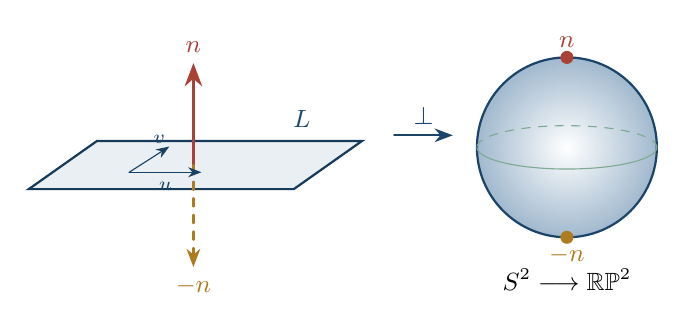
\begin{tikzpicture}[>=Stealth,line cap=round,scale=1.02]
 \filldraw[fill=manifoldblue!10,draw=manifoldblue!65!black,thick]
 (-4.6,-.52)--(-1.3,-.52)--(-.45,.08)--(-3.75,.08)--cycle;
 \draw[->,very thick,manifoldred] (-2.55,-.22)--(-2.55,1.05)
   node[above,font=\small] {$n$};
 \draw[->,thick,manifoldgold!85!black,dashed]
   (-2.55,-.22)--(-2.55,-1.49)
   node[below,font=\small] {$-n$};
 \node[font=\small,manifoldblue!80!black] at (-1.2,.35) {$L$};
 \draw[->,manifoldblue!70!black] (-3.35,-.31)--(-2.45,-.31)
   node[midway,below,font=\scriptsize] {$u$};
 \draw[->,manifoldblue!70!black] (-3.35,-.31)--(-2.85,.01)
   node[near end,above,font=\scriptsize] {$v$};
 \shade[inner color=white,outer color=manifoldblue!43] (2.1,0) circle (1.12);
 \draw[manifoldblue!75!black,thick] (2.1,0) circle (1.12);
 \draw[manifoldgreen!65,thin] (.98,0) arc[start angle=180,end angle=360,x radius=1.12,y radius=.27];
 \draw[manifoldgreen!65,thin,dashed] (3.22,0)
   arc[start angle=0,end angle=180,x radius=1.12,y radius=.27];
 \fill[manifoldred] (2.1,1.12) circle (2.3pt)
   node[above,font=\small] {$n$};
 \fill[manifoldgold!85!black] (2.1,-1.12) circle (2.3pt)
   node[below,font=\small] {$-n$};
 \draw[->,manifoldblue!75!black,thick] (-.05,.15)--(.68,.15)
   node[midway,above,font=\small] {$\perp$};
 \node[font=\small] at (2.1,-1.65) {$S^2\longrightarrow\mathbb{RP}^2$};
\end{tikzpicture}
\caption{Orientacja płaszczyzny w $\R^3$ wybiera jedną z
dwóch jednostkowych normalnych. Zapomnienie orientacji
utożsamia punkty antypodyczne $n$ i $-n$ na sferze.}
\label{fig:grass-normalne}
\end{figure}

\begin{stwierdzenie}[Bazy ortonormalne i przestrzeń ilorazowa]
\label{prop:grass-stiefel}
Niech $V_k(\R^n)$ będzie zbiorem uporządkowanych
ortonormalnych $k$-ramek $(v_1,\ldots,v_k)$.
Odwzorowanie $(v_i)\mapsto\operatorname{span}(v_i)$ ma
włókna izomorficzne z $\mathrm O(k)$.
Ponadto, jako gładkie przestrzenie,
\[
 \operatorname{Gr}_k(\R^n)
   \cong\mathrm O(n)/(\mathrm O(k)\times\mathrm O(n-k)),
\quad
 \operatorname{Gr}_k(\C^n)
   \cong\mathrm U(n)/(\mathrm U(k)\times\mathrm U(n-k)).
\]
\end{stwierdzenie}
\begin{proof}
Dwie ramki wyznaczają tę samą $k$-płaszczyznę wtedy
i tylko wtedy, gdy zmiana bazy między nimi należy do
$\mathrm O(k)$. Wykonując ortonormalizację Grama--Schmidta
na wektorach $u_i+Au_i$ z mapy wykresowej, dostajemy
gładki lokalny wybór ramki; włókna są więc lokalnie
kopiami $\mathrm O(k)$. Grupa $\mathrm O(n)$ działa
tranzytywnie na płaszczyznach: wybieramy bazy ortonormalne
dwóch płaszczyzn, uzupełniamy je do baz $\R^n$ i bierzemy
odwzorowanie przenoszące pierwszą pełną bazę na drugą.
Element zachowujący standardowe $\R^k$ zachowuje też
jego dopełnienie prostopadłe, czyli ma postać blokową
$\mathrm{diag}(B,C)$ z $B\in\mathrm O(k)$,
$C\in\mathrm O(n-k)$. To daje pierwszy iloraz.
Wyjaśnijmy gładką strukturę ilorazu. W rozkładzie ortogonalnym
$P\oplus Q$ uzupełniamy ramkę wykresu przez ramkę
$\Gamma(-A^*)\subset Q\oplus P$ jego dopełnienia prostopadłego:
jej wektory mają postać $-A^*w+w$, $w\in Q$.
Ortonormalizacja obu ramek daje macierz $s(A)\in\mathrm O(n)$
zależną gładko od $A$. Każda macierz ortogonalna nad tą mapą
ma jednoznaczną postać $s(A)\operatorname{diag}(B,C)$.
Parametr $A$ odzyskujemy z obrazu pierwszych $k$ kolumn,
a bloki $B,C$ z iloczynu $s(A)^{-1}O$. Daje to lokalny
produkt i jego gładką odwrotność; po podzieleniu przez bloki
pozostaje dokładnie mapa wykresowa grassmannianu.
Argument dla $\C$ jest taki sam, z bazami unitarnymi,
sprzężeniem hermitowskim i grupą $\mathrm U(n)$.
\end{proof}

Iloczyn zewnętrzny z Sekcji~\ref{sec:algebra-zewnetrzna}
pozwala zapisać $k$-płaszczyznę jednym wielowektorem,
określonym z dokładnością do niezerowego skalara.

\begin{twierdzenie}[Zanurzenie Plückera]
\label{thm:grass-plucker}
Jeśli $(v_1,\ldots,v_k)$ jest bazą $L$, to wzór
\begin{equation}\label{eq:plucker}
 \mathrm{Pl}(L):=[v_1\wedge\cdots\wedge v_k]
 \in\mathbb P(\Lambda^k V)
\end{equation}
określa gładkie zanurzenie
$\operatorname{Gr}_k(V)\hookrightarrow\mathbb P(\Lambda^k V)$.
Nawias $[\xi]$ oznacza prostą $\mathbb K\xi$,
$\xi\ne0$. Obraz składa się dokładnie z klas
niezerowych \emph{wielowektorów prostych}.
\end{twierdzenie}
\begin{proof}
Zmiana bazy $(v_i)$ macierzą $C$ mnoży iloczyn
zewnętrzny przez $\det C\ne0$ na mocy
Twierdzenia~\ref{thm:det-wlasnosci}, więc klasa
projektowa jest dobrze określona. Jeżeli
$\xi=v_1\wedge\cdots\wedge v_k\ne0$, to
\[
 L=\{w\in V:w\wedge\xi=0\}.
\]
Wektory z $L$ dają zero przez powtórzenie czynnika.
Jeśli $w\notin L$, rodzina $(v_1,\ldots,v_k,w)$
jest liniowo niezależna; po uzupełnieniu do bazy
Twierdzenie~\ref{thm:wedge-baza} mówi, że jej
iloczyn zewnętrzny jest niezerowy. Zatem
$\mathrm{Pl}(L)$ wyznacza $L$ jednoznacznie.

Pokażmy, skąd bierze się gładki odwrotny wzór na obrazie.
W mapie $V=P\oplus Q$ wybierzmy bazy
$e_1,\ldots,e_k$ przestrzeni $P$ oraz
$e_{k+1},\ldots,e_n$ przestrzeni $Q$ i zapiszmy
$Ae_j=\sum_{a=1}^{n-k}a_{aj}e_{k+a}$.
W wielowektorze
$\xi_A=(e_1+Ae_1)\wedge\cdots\wedge(e_k+Ae_k)$
współczynnik $p_{1\cdots k}$ wynosi $1$.
Współczynnik przy
$e_1\wedge\cdots\wedge\widehat{e_j}\wedge\cdots
\wedge e_k\wedge e_{k+a}$ wynosi
$(-1)^{k-j}a_{aj}$: przesuwamy $e_{k+a}$
przez $k-j$ późniejszych czynników.
Z ilorazów tych współczynników przez $p_{1\cdots k}$
odzyskujemy wszystkie $a_{aj}$.
W ogólnej mapie projektowej dzielimy przez
odpowiedni niezerowy współczynnik $p_I$.
Odwzorowanie~\eqref{eq:plucker} jest więc gładkie.
Wzory odzyskujące $a_{aj}$ są określone na całym otwartym
zbiorze przestrzeni projektowej $p_{1\cdots k}\ne0$, nie tylko
na obrazie. Ich złożenie z $\mathrm{Pl}$ jest mapą identyczną
w parametrach $A$; różniczkowanie daje lewą odwrotność różniczki
$\mathrm{Pl}$, która jest zatem injektywna.
Otrzymaliśmy immersję. Ponieważ grassmannian jest zwarty,
a przestrzeń projektowa Hausdorffa, ciągła injekcja jest
homeomorfizmem na obraz. To daje zanurzenie i domkniętość obrazu.
\end{proof}

\begin{przyklad}[Relacja Plückera dla $\operatorname{Gr}_2(\R^4)$]
Zapiszmy $\xi=\sum_{1\leq i<j\leq4}p_{ij}e_i\wedge e_j$.
Rozwinięcie $\xi\wedge\xi$ daje
\begin{equation}\label{eq:plucker-24}
 \xi\wedge\xi=
 2(p_{12}p_{34}-p_{13}p_{24}+p_{14}p_{23})
   e_1\wedge e_2\wedge e_3\wedge e_4.
\end{equation}
Jeżeli $\xi=u\wedge v$, to $\xi\wedge\xi=0$,
więc współczynniki spełniają relację w nawiasie.
Odwrotnie, dla $\xi\ne0$ z taką relacją możemy
przestawić współrzędne tak, by $p_{12}\ne0$.
Po podzieleniu przez $p_{12}$ ustawiamy w wykresie
$e_1+ae_3+ce_4$, $e_2+be_3+de_4$ liczby
$b=p_{13}/p_{12}$, $d=p_{14}/p_{12}$,
$a=-p_{23}/p_{12}$, $c=-p_{24}/p_{12}$.
Pięć współczynników się zgadza z definicji,
a szósty jest równy $ad-bc=p_{34}/p_{12}$
właśnie dzięki relacji. To dowodzi również
wystarczalności. Na przykład
$e_1\wedge e_2+e_3\wedge e_4$ ma
$p_{12}p_{34}=1$ i pozostałe wyrazy zerowe,
więc nie jest wielowektorem prostym, zgodnie
z wcześniejszym Przykładem w
Sekcji~\ref{sec:baza-zewnetrzna}.
\end{przyklad}

\begin{twierdzenie}[Odwzorowanie Gaussa i wiązka styczna]
\label{thm:grass-gauss}
Niech $M^m\subset\R^N$ będzie gładką podrozmaitością.
Przypisanie
$G(p)=T_pM\in\operatorname{Gr}_m(\R^N)$
jest gładkim \emph{odwzorowaniem Gaussa}. Wiązki
$TM$ i normalna $\nu M$ są odpowiednio
cofnięciami $G^*\gamma^m$ i $G^*\mathcal Q$
z~\eqref{eq:grass-ciag}.
\end{twierdzenie}
\begin{proof}
W mapie podrozmaitości zapisujemy jej parametryzację
$F:U\subset\R^m\to\R^N$. Wektory
$\partial_iF(x)$ tworzą gładką bazę $T_{F(x)}M$.
W pobliżu ustalonego punktu pewien minor $m\times m$
macierzy $\dd F$ pozostaje niezerowy. W odpowiadającym
mu rozkładzie $\R^N=P\oplus Q$ przestrzeń
$T_{F(x)}M$ jest wykresem macierzy
$A(x)=D_QF(x)(D_PF(x))^{-1}$,
gładkiej w $x$. Stąd $G$ jest gładka.
Włókno $(G^*\gamma^m)_p$ to z definicji
$\gamma^m_{G(p)}=T_pM$; lokalne ramki po obu
stronach są tymi samymi $\partial_iF$.
Włókno $(G^*\mathcal Q)_p$ to
$\R^N/T_pM$, czyli $\nu_pM$ z
Przykładu o wiązce normalnej w Sekcji o podrozmaitościach
Rozdziału~\ref{ch:rozmaitosci}.
Zgodność lokalnych trywializacji daje oba
izomorfizmy wiązek.
\end{proof}

\begin{uwaga}[Dlaczego wiązka tautologiczna jest uniwersalna?]
Na zwartej rozmaitości każdą gładką wiązkę $E$
rzędu $k$ można umieścić w trywialnej wiązce
$M\times\R^N$ dla pewnego $N$.
Oto konstrukcja. Wybieramy skończone pokrycie
trywializujące $U_i$, jego mniejsze podpokrycie
oraz funkcje gładkie $\beta_i$ o nośnikach w $U_i$,
takie że dla każdego $p$ co najmniej jedna
$\beta_i(p)$ jest niezerowa. Jeśli $[v]_i\in\R^k$
oznacza współrzędne $v\in E_p$ na $U_i$,
definiujemy różnowartościowe odwzorowanie liniowe w $v$
\[
 j_p(v)=\bigl(\beta_1(p)[v]_1,\ldots,
                  \beta_r(p)[v]_r\bigr)\in\R^{kr},
\]
przyjmując wartość $0$ dla bloku poza $U_i$.
Podparcie $\beta_i$ wewnątrz $U_i$ zapewnia
gładkość po przedłużeniu zerem; co najmniej
jeden niezerowy blok zapewnia iniektywność $j_p$.
Obrazy $j_p(E_p)$ zmieniają się gładko, ponieważ
lokalnie tworzą kolumny macierzy gładkiej i
stałego rzędu $k$, a więc definiują odwzorowanie
$f:M\to\operatorname{Gr}_k(\R^{kr})$.
Wprost z definicji włókien mamy
$E\cong f^*\gamma^k$. Ta konkretna konstrukcja
wyjaśnia użyteczność grassmannianów dla topologii
wiązek; nie potrzebuje jeszcze teorii klas
charakterystycznych.
\end{uwaga}

\section{Algebra Clifforda: iloczyn i dowód wymiaru}
\label{sec:clifford}

Od tego miejsca $V$ jest rzeczywistą przestrzenią
euklidesową wymiaru $n$ z iloczynem skalarnym
$\langle\cdot,\cdot\rangle$ i normą
$\|v\|^2=\langle v,v\rangle$. Algebra zewnętrzna
pamięta zorientowane pola: $v\wedge v=0$.
Algebra Clifforda pamięta ponadto \emph{długość}:
kwadrat wektora jest skalarem $-\|v\|^2$.
Przyjmujemy konsekwentnie ten znak minus;
w literaturze spotyka się również konwencję przeciwną.

\begin{definicja}[Algebra Clifforda]
\index{algebra clifforda@Algebra Clifforda}
\label{def:clifford}
Niech $I_q$ będzie ideałem obustronnym algebry
tensorowej $T(V)$ z Definicji~\ref{def:algebra-tensorowa},
generowanym przez
$v\otimes v+\|v\|^2\,1$ dla wszystkich $v\in V$.
\emph{Algebra Clifforda} to
\[
 \operatorname{Cl}(V):=T(V)/I_q.
\]
Obraz $v\in V$ oznaczamy nadal $v$,
a mnożenie w ilorazie zapisujemy bez symbolu $\otimes$.
Z definicji $v^2=-\|v\|^2\,1$.
\end{definicja}

Po usunięciu z relacji składnika $\|v\|^2\,1$
otrzymujemy algebrę zewnętrzną
(Definicja~\ref{def:algebra-zewnetrzna}).
Tak więc obie algebry startują z tej samej algebry
tensorowej; zmieniamy tylko relację, przez którą
dzielimy. W algebrze Clifforda nie można zachować
zwykłego stopnia tensorowego: relacja utożsamia
wyraz stopnia $2$ ze skalarem stopnia $0$.
Pozostaje rozróżnienie stopnia \emph{parzystego}
i \emph{nieparzystego}, bo oba wyrazy relacji
mają tę samą parzystość.

\begin{twierdzenie}[Relacja Clifforda i własność uniwersalna]
\label{thm:cliff-relacje}
Dla $v,w\in V$ w $\operatorname{Cl}(V)$ zachodzi
\begin{equation}\label{eq:cliff-relacja}
 vw+wv=-2\langle v,w\rangle\,1.
\end{equation}
Jeżeli $\mathcal A$ jest łączną algebrą rzeczywistą
z jedynką, a $f:V\to\mathcal A$ jest liniowa i spełnia
$f(v)^2=-\|v\|^2 1_{\mathcal A}$ dla każdego $v$,
to istnieje dokładnie jeden homomorfizm algebr
$\widehat f:\operatorname{Cl}(V)\to\mathcal A$
przedłużający $f$.
\end{twierdzenie}
\begin{proof}
Rozwijając $(v+w)^2$ na dwa sposoby, otrzymujemy
\[
 v^2+vw+wv+w^2=-\|v+w\|^2\,1
  =-(\|v\|^2+\|w\|^2+2\langle v,w\rangle)\,1.
\]
Po odjęciu $v^2=-\|v\|^2 1$ i
$w^2=-\|w\|^2 1$ zostaje~\eqref{eq:cliff-relacja}.
Z Twierdzenia~\ref{thm:algebra-tensorowa-universal}
odwzorowanie $f$ przedłuża się jednoznacznie do homomorfizmu
$F:T(V)\to\mathcal A$. Dla każdego generatora ideału
$I_q$ mamy
$F(v\otimes v+\|v\|^2 1)
 =f(v)^2+\|v\|^2 1_{\mathcal A}=0$.
Jądro homomorfizmu jest ideałem, więc zawiera $I_q$.
Wobec tego wzór $\widehat f([t])=F(t)$
nie zależy od przedstawiciela $t\in T(V)$
i wyznacza żądany homomorfizm na ilorazie.
Jednoznaczność wynika stąd, że $V$ i jedynka
generują $\operatorname{Cl}(V)$.
\end{proof}

Przy bazie ortonormalnej $(e_1,\ldots,e_n)$
relacja~\eqref{eq:cliff-relacja} mówi
\begin{equation}\label{eq:cliff-orto}
 e_i^2=-1,\qquad e_ie_j=-e_je_i\quad(i\ne j).
\end{equation}
Stąd każdy iloczyn generatorów można uporządkować
rosnąco, redukując powtórzone indeksy.
Trudniejszą częścią jest wykazanie, że tak otrzymane
wyrazy nie mają dodatkowych relacji.

\begin{twierdzenie}[Baza algebry Clifforda]
\label{thm:cliff-baza}
Dla bazy ortonormalnej $e_1,\ldots,e_n$ elementy
\[
 1,\qquad e_{i_1}\cdots e_{i_r}
 \quad(1\leq i_1<\cdots<i_r\leq n,\ 1\leq r\leq n)
\]
stanowią bazę $\operatorname{Cl}(V)$. Zatem
$\dim_\R\operatorname{Cl}(V)=2^n$.
Dla $n\geq1$ części parzysta i nieparzysta mają
po $2^{n-1}$ wymiarów.
\end{twierdzenie}
\begin{proof}
\emph{Rozpinanie.} Obrazy słów $v_1\cdots v_r$
rozpinają iloraz $T(V)/I_q$. Po rozwinięciu każdego
$v_j$ w bazie wystarczą słowa z liter $e_i$.
Równości~\eqref{eq:cliff-orto} pozwalają zamienić
każde dwie sąsiednie różne litery (ze zmianą znaku)
i usunąć parę równych liter ($e_i^2=-1$).
Powtarzając te operacje, dostajemy kombinację
iloczynów o rosnących, różnych indeksach.

\emph{Niezależność.} Skorzystamy z algebry zewnętrznej
$\Lambda(V)$ z Rozdziału~\ref{ch:algebra-tensorowa}.
Na niej określmy dwie operacje:
\[
 \varepsilon(v)\omega:=v\wedge\omega,\qquad
 \iota_v(w_1\wedge\cdots\wedge w_r)
 :=\sum_{j=1}^r(-1)^{j-1}
   \langle v,w_j\rangle\,
   w_1\wedge\cdots\wedge\widehat{w_j}
       \wedge\cdots\wedge w_r .
\]
Kreska nad $w_j$ oznacza pominięcie tego czynnika;
przyjmujemy $\iota_v(1)=0$.
Wzór na $\iota_v$ jest wieloliniowy i alternujący
w $w_j$: przy zamianie dwóch sąsiednich argumentów składniki
pomijające inny argument zmieniają znak przez antysymetrię iloczynu
zewnętrznego, a dwa pozostałe zamieniają się miejscami z przeciwnymi
znakami. Zatem własność uniwersalna
z Twierdzenia~\ref{thm:wedge-multilinear}
zapewnia, że operator jest dobrze określony.
Bezpośrednio z tego wzoru otrzymujemy
\[
 \iota_v(w\wedge\omega)
  =\langle v,w\rangle\omega-w\wedge\iota_v\omega.
\]
Pierwszy składnik powstaje przy usunięciu pierwszego
czynnika; pozostałe mają o jeden minus więcej niż
w $\iota_v\omega$. Usunięcie dwóch czynników
w dwóch przeciwnych kolejnościach daje składniki
o przeciwnych znakach, zatem $\iota_v^2=0$.
Również $\varepsilon(v)^2=0$, bo $v\wedge v=0$.
Jeżeli $c(v):=\varepsilon(v)-\iota_v$, to
\[
 c(v)^2
 =-\bigl(\varepsilon(v)\iota_v
          +\iota_v\varepsilon(v)\bigr)
 =-\|v\|^2\id_{\Lambda(V)}.
\]
Własność uniwersalna z poprzedniego twierdzenia
daje więc reprezentację
$c:\operatorname{Cl}(V)\to\operatorname{End}_\R(\Lambda V)$.
Przyłóżmy ją do $1\in\Lambda^0V$.
Dla różnych ortonormalnych $e_{i_j}$ wszystkie
kontrakcje pojawiające się podczas kolejnego
działania znikają: nowy $e_{i_j}$ jest prostopadły
do wcześniej utworzonych czynników. Stąd
\[
 c(e_{i_1}\cdots e_{i_r})\,1
    =e_{i_1}\wedge\cdots\wedge e_{i_r},\qquad
 c(1)\,1=1.
\]
Prawa strona przebiega bazę $\Lambda(V)$ z
Twierdzenia~\ref{thm:wedge-baza}. Jeśli kombinacja
uporządkowanych słów znikałaby w algebrze Clifforda,
jej działanie na $1$ dawałoby zerową kombinację
\emph{różnych} wektorów tej bazy. Wszystkie
współczynniki muszą więc być zerowe.
Słów o $r$ indeksach jest $\binom nr$;
sumując po $r$ otrzymujemy $2^n$.
Wreszcie bijekcja $I\mapsto I\triangle\{1\}$
zamienia podzbiory parzystej i nieparzystej
liczności, co dowodzi równości ich liczby.
\end{proof}

\begin{uwaga}[Podobne przestrzenie, różne mnożenia]
\label{rem:cliff-zewnetrzna}
Istnieje kanoniczny izomorfizm \emph{przestrzeni liniowych}
$\Lambda V\cong\operatorname{Cl}(V)$: wysyła
$v_1\wedge\cdots\wedge v_r$ na antysymetryzację
$\frac1{r!}\sum_{\sigma\in S_r}\operatorname{sgn}(\sigma)
 v_{\sigma(1)}\cdots v_{\sigma(r)}$.
Jest dobrze określony, bo wyrażenie jest alternujące;
na bazowych wektorach ortonormalnych daje
$e_{i_1}\cdots e_{i_r}$, więc poprzednie twierdzenie
zapewnia odwracalność. Nie jest to jednak izomorfizm
algebr: w $\Lambda V$ mamy $v\wedge v=0$,
a w $\operatorname{Cl}(V)$ mamy
$v^2=-\|v\|^2$. To wyjaśnia, dlaczego obie
przestrzenie mają wymiar $2^n$, choć kodują
inne mnożenia.
\end{uwaga}

\begin{przyklad}[Wymiary $0$, $1$ i $2$]
Dla $V=0$ otrzymujemy $\operatorname{Cl}(0)=\R$.
W wymiarze $1$, przy $e_1^2=-1$, każdy element
ma postać $a+be_1$ i mnoży się jak liczba
$a+bi\in\C$. Stąd $\operatorname{Cl}(\R)\cong\C$
\emph{jako algebra rzeczywista}.
W wymiarze $2$ baza $(1,e_1,e_2,e_1e_2)$
spełnia dokładnie relacje kwaternionów:
$e_1\leftrightarrow i$, $e_2\leftrightarrow j$,
$e_1e_2\leftrightarrow k$, zatem
$\operatorname{Cl}(\R^2)\cong\mathbb H$.
Na przykład $(e_1+2e_2)^2=-5$, podczas gdy
$(e_1+2e_2)\wedge(e_1+2e_2)=0$
w algebrze zewnętrznej. Porównujemy więc kwadraty tego samego wektora.
\end{przyklad}

\begin{stwierdzenie}[Iloczyn wektorów: skalar i dwuwektor]
\label{prop:cliff-wedge}
Przez powyższy izomorfizm przestrzeni liniowych
iloczyn Clifforda dwóch wektorów rozkłada się na
\begin{equation}\label{eq:cliff-rozdzial}
 vw=-\langle v,w\rangle
       +\tfrac12(vw-wv)
 \quad\longleftrightarrow\quad
 -\langle v,w\rangle+v\wedge w.
\end{equation}
\end{stwierdzenie}
\begin{proof}
Suma $vw+wv$ jest równa
$-2\langle v,w\rangle$ z~\eqref{eq:cliff-relacja}.
Dodając połowę tej sumy do połowy różnicy,
odzyskujemy $vw$. Antysymetryzacja
$v\wedge w\mapsto\tfrac12(vw-wv)$
jest przypadkiem stopnia $2$ opisanym w
poprzedniej uwadze.
\end{proof}

\begin{figure}[!htbp]
\centering
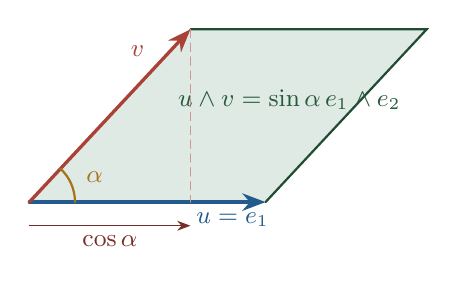
\begin{tikzpicture}[>=Stealth,line cap=round,scale=1.0]
 \coordinate (O) at (0,0);
 \coordinate (U) at (3.0,0);
 \coordinate (W) at ({3*cos(47)},{3*sin(47)});
 \coordinate (UW) at ({3+3*cos(47)},{3*sin(47)});
 \fill[manifoldgreen!16] (O)--(U)--(UW)--(W)--cycle;
 \draw[manifoldgreen!60!black,thick] (U)--(UW)--(W);
 \draw[->,manifoldblue,very thick] (O)--(U)
  node[pos=.86,below,font=\small] {$u=e_1$};
 \draw[->,manifoldred,very thick] (O)--(W)
  node[pos=.78,above left,font=\small] {$v$};
 \draw[densely dashed,manifoldred!55] (W)--({3*cos(47)},0);
 \draw[->,manifoldred!70!black] (0,-.3)--({3*cos(47)},-.3)
  node[midway,below,font=\small] {$\cos\alpha$};
 \draw[manifoldgold!80!black,thick] (.58,0)
  arc[start angle=0,end angle=47,radius=.58];
 \node[manifoldgold!80!black,font=\small] at (.83,.32) {$\alpha$};
 \node[manifoldgreen!70!black,font=\small] at (3.3,1.3)
  {$u\wedge v=\sin\alpha\,e_1\wedge e_2$};
\end{tikzpicture}
\caption{Dla jednostkowych $u=e_1$ i
$v=\cos\alpha\,e_1+\sin\alpha\,e_2$ iloczyn Clifforda
$uv=-\cos\alpha+\sin\alpha\,e_1e_2$ łączy
ujemny iloczyn skalarny ze zorientowanym polem.}
\label{fig:cliff-iloczyn}
\end{figure}

\section{Od odbić do grupy Spin}
\label{sec:spin-grupa}

Ustalmy najpierw dwie operacje na algebrze Clifforda.
Zmiana każdego $v$ na $-v$ zachowuje relacje definiujące,
więc daje automorfizm $\alpha$, z $\alpha^2=\id$.
Jego przestrzenie własne dla $+1$ i $-1$ są rozpięte
odpowiednio przez słowa parzyste i nieparzyste; dowód bazy
pokazuje, że ich suma jest prosta.
Drugą operacją jest \emph{rewersja}, oznaczana tyldą:
\[
 \widetilde{v_1\cdots v_r}=v_r\cdots v_1,\qquad
 \widetilde 1=1,
\]
przedłużona liniowo. Jest dobrze określona na ilorazie:
odwracanie słów w $T(V)$ ustala każdy generator
$v\otimes v+\|v\|^2 1$, a element $a(v\otimes v+\|v\|^2 1)b$
wysyła na $\widetilde b(v\otimes v+\|v\|^2 1)\widetilde a$,
nadal należący do ideału. Zatem
$\widetilde{st}=\widetilde t\,\widetilde s$ i
$\widetilde{\widetilde s}=s$, niezależnie od zapisu $s$ jako sumy słów.

Odbicie względem hiperpłaszczyzny prostopadłej
do jednostkowego $u\in V$ ma wzór
\begin{equation}\label{eq:spin-odbicie}
 r_u(v)=v-2\langle u,v\rangle u.
\end{equation}
Rozkład $v=\langle u,v\rangle u+w$, $w\perp u$,
pokazuje, że $r_u$ odwraca składową równoległą do $u$
i zostawia składową $w$. Jego wyznacznik jest równy $-1$.
Relacja Clifforda daje zaskakujący opis tego odbicia:
ponieważ $u^2=-1$, mamy $u^{-1}=-u$ i
\[
 -uvu^{-1}=uvu
 =-\langle u,v\rangle u+w
 =r_u(v).
\]

\begin{definicja}[Grupa Pin]
\label{def:pin-grupa}
\index{grupa pin@Grupa Pin}
Dla euklidesowej przestrzeni $V$ grupą $\operatorname{Pin}(V)$
nazywamy podgrupę odwracalnych elementów $\operatorname{Cl}(V)$
złożoną ze wszystkich skończonych iloczynów wektorów
jednostkowych; dopuszczamy pusty iloczyn $1$.
W odróżnieniu od grupy Spin dopuszczamy także nieparzystą
liczbę czynników. Dla $s\in\operatorname{Pin}(V)$ określamy
\[
 \rho_{\mathrm{Pin}}(s)(v):=\alpha(s)v s^{-1},
 \qquad v\in V,
\]
gdzie $\alpha$ zmienia znak każdego wektora, jak wyżej.
\end{definicja}

Wzór jest skręconym sprzężeniem: dla jednostkowego $u$
daje $\rho_{\mathrm{Pin}}(u)(v)=-uvu^{-1}=r_u(v)$.
Zatem pojedynczy wektor reprezentuje odbicie, a jego parzysty
iloczyn reprezentuje obrót. Na przykład w $\R^2$ element
$e_1\in\operatorname{Pin}(2)$ daje odbicie w prostej
$e_1^\perp$, podczas gdy $e_1e_2$ daje obrót o pół obiegu.
Przy przyjętej relacji $u^2=-\|u\|^2$ grupa ta bywa
oznaczana $\operatorname{Pin}^{-}(n)$; znak rozróżnia dwie
konwencje algebry Clifforda.

\begin{definicja}[Grupa Spin]
\index{grupa spin@Grupa Spin}
\label{def:spin-grupa}
Niech $n=\dim V\geq2$. \emph{Grupą spinową}
$\operatorname{Spin}(V)$ nazywamy podgrupę
odwracalnych elementów $\operatorname{Cl}(V)$,
składającą się z iloczynów \emph{parzystej}
liczby wektorów jednostkowych:
\[
 \operatorname{Spin}(V)
 :=\{u_1\cdots u_{2r}:\|u_j\|=1,\ r\geq0\}.
\]
Pusty iloczyn to $1$. Skrót
$\operatorname{Spin}(n)$ oznacza
$\operatorname{Spin}(\R^n)$ ze standardową metryką.
Dla $s\in\operatorname{Spin}(V)$ określamy
$\rho(s)v:=svs^{-1}$.
Topologię na grupie bierzemy z jej włączenia do skończenie
wymiarowej przestrzeni $\operatorname{Cl}(V)$. Gładką strukturę
zgodną z tym włączeniem uzasadnimy w dowodzie nakrycia.
\end{definicja}

Zbiór w definicji jest grupą: iloczyn dwóch słów
parzystych jest parzysty, a odwrotność słowa
$u_1\cdots u_{2r}$ to
$(-u_{2r})\cdots(-u_1)$, ponownie słowo parzyste
złożone z wektorów jednostkowych.
Każdy jego czynnik ma dobrze określoną odwrotność.

\begin{twierdzenie}[Dwukrotne nakrycie grupy obrotów]
\label{thm:spin-nakrycie}
Przypisanie $\rho$ jest surjektywnym homomorfizmem
\[
 \rho:\operatorname{Spin}(n)\longrightarrow\mathrm{SO}(n),
 \qquad\ker\rho=\{1,-1\}.
\]
Jest gładkim dwukrotnym nakryciem: każdy obrót
ma dokładnie dwa podniesienia $s$ i $-s$.
\end{twierdzenie}
\begin{proof}
\emph{Dlaczego obrazem jest obrót?}
Dla słowa $s=u_1\cdots u_{2r}$ zastosujmy
wzór na odbicie do kolejnych czynników.
W odwzorowaniu $v\mapsto-u v u^{-1}$ pojawia się
jedno odbicie $r_u$; przy parzystej liczbie
czynników wszystkie minusy się znoszą i
\[
 \rho(s)=r_{u_1}\circ\cdots\circ r_{u_{2r}}.
\]
To złożenie zachowuje iloczyn skalarny i ma
wyznacznik $(-1)^{2r}=1$. Ponieważ
$\rho(st)(v)=s(tvt^{-1})s^{-1}$,
$\rho$ jest homomorfizmem do $\mathrm{SO}(n)$.

\emph{Dlaczego jest surjektywna?}
Pokażmy elementarnie, że każdą izometrię liniową
można zapisać jako iloczyn odbić. Weźmy bazę
ortonormalną $e_1,\ldots,e_n$ i $A\in\mathrm O(n)$.
Jeśli $Ae_1\ne e_1$, to dla
$u=(Ae_1-e_1)/\|Ae_1-e_1\|$ rachunek z
\eqref{eq:spin-odbicie} daje $r_u(Ae_1)=e_1$:
licznik iloczynu
$\langle Ae_1-e_1,Ae_1\rangle$ to
$1-\langle Ae_1,e_1\rangle$, a kwadrat
mianownika to $2(1-\langle Ae_1,e_1\rangle)$.
Jeśli $Ae_1=e_1$, pomijamy ten krok.
Nowa izometria zachowuje $e_1$, więc działa
na $e_1^\perp$. Powtarzamy argument dla $e_2$
w tym dopełnieniu, potem dla $e_3$, itd.
Po skończenie wielu krokach otrzymujemy
identyczność. Zapisujemy więc $A$ jako
iloczyn odbić. Ponieważ $\det A=1$, liczba
użytych odbić musi być parzysta; odpowiadający
im iloczyn jednostkowych $u_j$ jest szukanym
elementem $\operatorname{Spin}(n)$.

\emph{Dlaczego jądro ma tylko dwa elementy?}
Niech $s$ działa trywialnie na $V$. Wtedy
$se_j=e_js$ dla każdego wektora bazy ortonormalnej.
Rozwińmy $s$ w bazie z
Twierdzenia~\ref{thm:cliff-baza}, używając tylko
słów parzystej długości:
$s=\sum_{|I|\ {\rm parzyste}}a_I e_I$.
Dla parzystego niepustego $I$ i $j\in I$
relacja~\eqref{eq:cliff-orto} daje
$e_je_Ie_j^{-1}=-e_I$; gdy $j\notin I$,
otrzymujemy $+e_I$. Równość
$e_jse_j^{-1}=s$ dla \emph{wszystkich} $j$
wymusza więc $a_I=0$ dla każdego niepustego $I$.
Zatem $s=a\,1$. Aby ustalić $a$, odwróćmy
porządek wektorów w słowie:
$\widetilde s=u_{2r}\cdots u_1$.
Wtedy $s\widetilde s=(-1)^{2r}=1$,
bo wektory są jednostkowe i $u_i^2=-1$.
Dla skalarnego $s=a$ również $\widetilde s=a$,
stąd $a^2=1$. Oba znaki występują,
gdyż $-1=e_1e_1\in\operatorname{Spin}(n)$.

\emph{Dlaczego rzeczywiście jest to nakrycie?}
Pokażmy, że w pobliżu identyczności obroty mają
gładko wybrane podniesienie. Dla bliskich
jednostkowych $a,b$ połóżmy
\[
 R(a,b):=-\frac{a+b}{\|a+b\|}\,a
       =\frac{1-ba}{\|a+b\|}\in\operatorname{Spin}(n).
\]
Jest to iloczyn dwóch jednostkowych wektorów,
zależy gładko od $(a,b)$, spełnia $R(a,a)=1$
i przenosi $a$ na $b$: pierwsze odbicie w
hiperpłaszczyźnie do $a$ wysyła $a$ na $-a$,
drugie, o normalnej $(a+b)/\|a+b\|$, wysyła
$-a$ na $b$. Jeśli $A$ jest bliski identyczności,
stosujemy taki rotor, aby skorygować $Ae_1$ do
$e_1$. Otrzymany obrót zachowuje $e_1$.
W $e_1^\perp$ korygujemy następnie obraz
$e_2$, potem $e_3$, kończąc na $e_{n-1}$;
ostatni wektor jest ustalony dzięki wyznacznikowi
$1$. Każdy rotor zależy gładko od $A$
w niewielkim otoczeniu identyczności.
Odwrotność ich iloczynu daje gładką lokalną
sekcję $\sigma$ odwzorowania $\rho$.
Przy innym obrocie przenosimy to otoczenie
przez ustalony element z jego przeciwobrazu.
Jądro $\{\pm1\}$ oznacza, że przeciwobraz
takiego dostatecznie małego otoczenia jest
sumą rozłącznych kopii obrazu $\sigma$ i $-\sigma$.
Są one otwarte w $\operatorname{Spin}(n)$:
blisko $1$ dwie wartości $\pm\sigma(A)$
odróżnia znak współczynnika skalarnego
w algebrze Clifforda, a blisko pozostałych
punktów korzystamy z mnożenia przez
ustalone podniesienie. To jest dokładnie definicja
dwukrotnego nakrycia.
W ten sposób otrzymujemy także atlas gładki: na każdym płacie
używamy współrzędnych z $\mathrm{SO}(n)$ przeniesionych przez $\rho$.
Jest on zgodny z włączeniem do algebry Clifforda. Istotnie,
$\sigma$ jest gładka jako mapa do tej algebry, a pochodna
$\rho\circ\sigma=\id$ jest identycznością. Do różniczkowania
$\rho$ w otoczeniu płata wystarczy gładki wzór
$s\mapsto(v\mapsto\operatorname{pr}_V(svs^{-1}))$
na otwartym zbiorze elementów odwracalnych; na grupie Spin
rzut $\operatorname{pr}_V$ niczego nie zmienia.
Wynika stąd injektywność różniczki $\sigma$, więc płaty są
lokalnie podrozmaitościami algebry Clifforda. Mnożenie jest
dwuliniowe, a odwracanie gładkie: można je obliczać przez
odwracanie macierzy lewego mnożenia. Obie operacje ograniczają
się więc do gładkich operacji grupy Spin, a $\rho$ jest lokalnym dyfeomorfizmem.
\end{proof}

\begin{wniosek}[Nakrycie grupy ortogonalnej przez Pin]
\label{cor:pin-nakrycie}
Dla $n\geq2$ odwzorowanie
\[
 \rho_{\mathrm{Pin}}:\operatorname{Pin}(n)\longrightarrow
 \mathrm O(n)
\]
jest surjektywnym homomorfizmem o jądrze $\{1,-1\}$.
Jest gładkim dwukrotnym nakryciem, a przeciwobraz
$\mathrm{SO}(n)$ jest równy $\operatorname{Spin}(n)$.
\end{wniosek}
\begin{proof}
Automorfizm $\alpha$ jest multiplikatywny, więc
$\rho_{\mathrm{Pin}}(st)=\rho_{\mathrm{Pin}}(s)
\rho_{\mathrm{Pin}}(t)$. Każdy czynnik jednostkowy
daje odbicie. Rozkład izometrii na odbicia wykonano
w dowodzie Twierdzenia~\ref{thm:spin-nakrycie}; zapewnia
on surjektywność. Wyznacznik obrazu iloczynu $r$
wektorów wynosi $(-1)^r$. Parzyste słowa tworzą
zatem dokładnie przeciwobraz $\mathrm{SO}(n)$, czyli
$\operatorname{Spin}(n)$. Element jądra musi być parzysty,
a jądro na $\operatorname{Spin}(n)$ obliczono w tym samym
twierdzeniu jako $\{\pm1\}$. Lokalnie nad składową
$\mathrm{SO}(n)$ mamy już dwa gładkie płaty nakrycia Spin.
Mnożenie przez ustalony wektor jednostkowy przenosi je
na drugą składową $\mathrm O(n)$, co dowodzi ostatniej tezy.
\end{proof}

\begin{przyklad}[Dlaczego pojawia się połowa kąta?]
\label{prz:spin2}
W płaszczyźnie $B=e_1e_2$ spełnia $B^2=-1$.
Ponieważ część parzysta ma bazę $(1,B)$,
jej elementy mają postać $a+bB$. Dla słów
należących do $\operatorname{Spin}(2)$ równość
$s\widetilde s=1$ z poprzedniego dowodu daje
$a^2+b^2=1$. Odwrotnie, jeśli
$a=\cos t$, $b=\sin t$, to
\[
 a+bB=(-\cos t\,e_1-\sin t\,e_2)e_1,
\]
czyli iloczyn dwóch jednostkowych wektorów.
Grupa $\operatorname{Spin}(2)$ jest zatem okręgiem.
Połóżmy
\[
 s_\theta=\cos(\theta/2)+\sin(\theta/2)B.
\]
Korzystając z $Be_1=e_2$ i $Be_2=-e_1$,
obliczamy bez pomijania kroku
\[
 s_\theta e_1s_\theta^{-1}
 =(\cos^2\tfrac\theta2-\sin^2\tfrac\theta2)e_1
   +2\sin\tfrac\theta2\cos\tfrac\theta2\,e_2
 =\cos\theta\,e_1+\sin\theta\,e_2.
\]
Analogicznie obraz $e_2$ to
$-\sin\theta\,e_1+\cos\theta\,e_2$.
Jeden pełny obrót ma zatem podniesienie
$s_{2\pi}=-1$, a dopiero $s_{4\pi}=1$.
Po utożsamieniu obu grup z okręgiem odwzorowanie
$\rho$ ma postać $z\mapsto z^2$.
\end{przyklad}

\begin{figure}[!htbp]
\centering
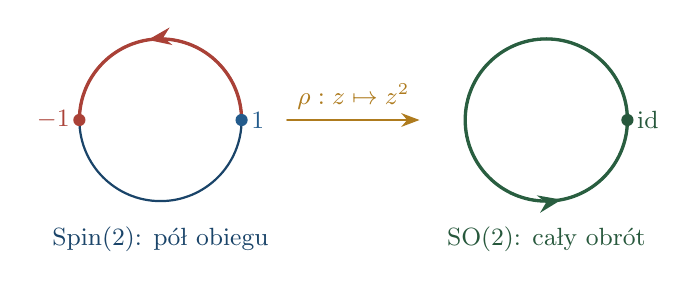
\begin{tikzpicture}[>=Stealth,line cap=round]
 \draw[manifoldblue!75!black,thick] (-2.45,0) circle (1.03);
 \draw[manifoldgreen!75!black,thick] (2.45,0) circle (1.03);
 \draw[manifoldred,very thick,postaction={decorate},
  decoration={markings,mark=at position .55 with {\arrow{Stealth}}}]
  (-1.42,0) arc[start angle=0,end angle=180,radius=1.03];
 \draw[manifoldgreen!75!black,very thick,postaction={decorate},
  decoration={markings,mark=at position .78 with {\arrow{Stealth}}}]
  (3.48,0) arc[start angle=0,end angle=360,radius=1.03];
 \fill[manifoldblue] (-1.42,0) circle (2.2pt)
  node[right,font=\small] {$1$};
 \fill[manifoldred] (-3.48,0) circle (2.2pt)
  node[left,font=\small] {$-1$};
 \fill[manifoldgreen!70!black] (3.48,0) circle (2.2pt)
  node[right,font=\small] {$\id$};
 \draw[->,thick,manifoldgold!85!black] (-.84,0)--(.84,0)
  node[midway,above,font=\small] {$\rho:z\mapsto z^2$};
 \node[font=\small,manifoldblue!75!black] at (-2.45,-1.52)
  {$\operatorname{Spin}(2)$: pół obiegu};
 \node[font=\small,manifoldgreen!70!black] at (2.45,-1.52)
  {$\mathrm{SO}(2)$: cały obrót};
\end{tikzpicture}
\caption{Droga od $1$ do $-1$ w $\operatorname{Spin}(2)$
rzutuje się na pełen obrót w $\mathrm{SO}(2)$.
Końce drogi są różne w grupie Spin, choć odpowiadają
temu samemu obrotowi.}
\label{fig:spin-dwukrotne}
\end{figure}

\begin{przyklad}[Trzy wymiary: kwaterniony]
\label{prz:spin3}
W $\operatorname{Cl}(\R^3)$ część parzysta ma bazę
$1,I=e_2e_3,J=e_3e_1,K=e_1e_2$.
Rachunek przy użyciu~\eqref{eq:cliff-orto} daje
$I^2=J^2=K^2=-1$ i $IJ=K$, $JK=I$, $KI=J$.
Jest to algebra kwaternionów $\mathbb H$.
Odwracanie kolejności czynników wysyła
$a+bI+cJ+dK$ na $a-bI-cJ-dK$,
więc $s\widetilde s=a^2+b^2+c^2+d^2$.
Każdy element $\operatorname{Spin}(3)$
jest zatem jednostkowym kwaternionem.
I odwrotnie, dowolny jednostkowy kwaternion
można zapisać jako $\cos t+\sin t\,B$,
gdzie $B$ jest jednostkowym dwuwektorem
w $\R^3$ (przypadki $\pm1$ są natychmiastowe).
Każdy taki $B$ jest iloczynem dwóch
prostopadłych wektorów jednostkowych. Aby to sprawdzić,
zapiszmy $B=b e_2e_3+c e_3e_1+d e_1e_2$ z $b^2+c^2+d^2=1$.
Wybierzmy jednostkowy $u\perp n=(b,c,d)$ i połóżmy
$v=n\times u$. Wtedy $u,v$ są ortonormalne i $u\times v=n$.
Współczynniki $u\wedge v$ w bazie
$(e_2\wedge e_3,e_3\wedge e_1,e_1\wedge e_2)$ są właśnie $(b,c,d)$,
więc $uv=B$. Z kolei
$\cos t+\sin t\,B$ jest także iloczynem dwóch
wektorów jednostkowych: jeśli $B=uv$ dla
$u\perp v$, to wprost z $vu=-uv$ i $u^2=-1$
otrzymujemy
\[
 (-\cos t\,u-\sin t\,v)u
     =\cos t+\sin t\,uv.
\]
Zatem $\operatorname{Spin}(3)\cong S^3$
jako grupa jednostkowych kwaternionów,
a $\rho:S^3\to\mathrm{SO}(3)$ utożsamia
parę $s,-s$.
\end{przyklad}

\section{Spinory: moduły algebry Clifforda}
\label{sec:spinory}

Wektor w $\R^n$ obraca się przez $\rho(s)\in\mathrm{SO}(n)$.
Spinor ma podlegać działaniu samego $s\in\operatorname{Spin}(n)$,
tak aby dwa podniesienia tego samego obrotu mogły
działać odmiennie. Do opisania wszystkich wymiarów
użyjemy liczb zespolonych. \emph{Zespolenie}
$\operatorname{Cl}^{\C}_n:=
\operatorname{Cl}(\R^n)\otimes_\R\C$
ma tę samą bazę uporządkowanych słów co algebra
rzeczywista, ale współczynniki zespolone.
Jego wymiar nad $\C$ wynosi $2^n$.

\begin{definicja}[Spinor zespolony]
\index{spinor zespolony@Spinor zespolony}
\label{def:spinor}
\emph{Moduł} algebry $A$ nad $\mathbb K$ to przestrzeń liniowa
$\Delta$ nad $\mathbb K$ z działaniem $A\times\Delta\to\Delta$
dwuliniowym nad $\mathbb K$ i zgodnym
z mnożeniem: $(ab)\psi=a(b\psi)$
oraz $1\psi=\psi$. Jest \emph{nieredukowalny},
jeśli $\Delta\ne0$ i nie ma właściwej niezerowej podprzestrzeni
zachowywanej przez wszystkie działania $a\in A$.
W tym rozdziale \emph{przestrzenią spinorów}
w wymiarze $n$ nazwiemy nieredukowalny zespolony
moduł $\Delta_n$ algebry $\operatorname{Cl}^{\C}_n$.
Jej element $\psi$ to spinor. Ograniczenie
działania do $\operatorname{Spin}(n)\subset
\operatorname{Cl}^{\C}_n$ jest
\emph{reprezentacją spinową}.
\end{definicja}

Słowo \emph{moduł} brzmi abstrakcyjnie, lecz tutaj
oznacza po prostu konkretne macierze $c(v)$
działające na kolumny $\psi$, z warunkiem
$c(v)^2=-\|v\|^2 I$. Działanie na całej algebrze
jest wtedy wyznaczone przez jej własność uniwersalną.
Przykładem modułu jest $\Lambda V$ z dowodu
Twierdzenia~\ref{thm:cliff-baza}, ale zwykle jest
on \emph{większy} niż nieredukowalna przestrzeń
spinorów. Nie należy więc utożsamiać automatycznie
wielowektora ze spinorem.

\begin{przyklad}[Macierze Pauliego]
\label{prz:pauli}
Niech
\[
 \sigma_1=\begin{pmatrix}0&1\\1&0\end{pmatrix},
 \quad
 \sigma_2=\begin{pmatrix}0&-i\\i&0\end{pmatrix},
 \quad
 \sigma_3=\begin{pmatrix}1&0\\0&-1\end{pmatrix}.
\]
Bezpośrednie mnożenie daje
$\sigma_i^2=I_2$ i
$\sigma_i\sigma_j=-\sigma_j\sigma_i$ przy $i\ne j$;
na przykład $\sigma_1\sigma_2=i\sigma_3$.
Macierze $c(e_j)=i\sigma_j$ spełniają więc
\[
 c(e_i)c(e_j)+c(e_j)c(e_i)=-2\delta_{ij}I_2.
\]
Dla $n=2$ wystarczą $c(e_1),c(e_2)$.
Ich iloczyn to $-i\sigma_3$, a cztery macierze
$I_2,i\sigma_1,i\sigma_2,-i\sigma_3$
są liniowo niezależne i rozpinają
$M_2(\C)$. Z wymiaru $4$ obu stron dostajemy
$\operatorname{Cl}^{\C}_2\cong M_2(\C)$.
Przestrzeń spinorów $\Delta_2=\C^2$
jest zwykłą przestrzenią kolumn długości $2$.
\end{przyklad}

\begin{twierdzenie}[Klasyfikacja zespolona i wymiar spinorów]
\label{thm:cliff-kompleks}
Dla $m\geq0$ istnieją izomorfizmy algebr
\begin{align}
 \operatorname{Cl}^{\C}_{2m}
   &\cong M_{2^m}(\C), \label{eq:cliff-complex-even}\\
 \operatorname{Cl}^{\C}_{2m+1}
   &\cong M_{2^m}(\C)\oplus M_{2^m}(\C).
   \label{eq:cliff-complex-odd}
\end{align}
Wobec tego nieredukowalny moduł zespolony
ma wymiar $2^{\lfloor n/2\rfloor}$.
Dla parzystego $n$ jest jeden taki moduł
z dokładnością do izomorfizmu, a dla
nieparzystego $n$ są dwa.
\end{twierdzenie}
\begin{proof}
W wymiarze $0$ algebra ma postać $\C$.
W wymiarze $1$ składa się z $a+be_1$ przy
$e_1^2=-1$, więc podstawienia $e_1=i$
i $e_1=-i$ dają
$\operatorname{Cl}^{\C}_1\cong\C\oplus\C$.
Przykład~\ref{prz:pauli} daje
$\operatorname{Cl}^{\C}_2\cong M_2(\C)$.

Wykażmy krok indukcyjny zwiększający wymiar o $2$.
Iloczyn tensorowy algebr wyposażamy tu w mnożenie
$(a\otimes A)(b\otimes B)=ab\otimes AB$, rozszerzone
dwuliniowo; własność uniwersalna iloczynu tensorowego zapewnia
jego poprawne określenie. Łączność sprawdzamy na tensorach
prostych, a jedynką jest $1\otimes I_2$.
Niech $e_1,\ldots,e_n$ będą generatorami
$\operatorname{Cl}^{\C}_n$. W algebrze
$\operatorname{Cl}^{\C}_n\otimes M_2(\C)$
weźmy $n+2$ elementów:
\[
 F_j=e_j\otimes\sigma_3\ (j\leq n),\qquad
 F_{n+1}=1\otimes i\sigma_1,\qquad
 F_{n+2}=1\otimes i\sigma_2.
\]
Każdy $F_j^2=-1$. Dwa różne elementy
antykomutują: dla $j,\ell\leq n$ wynika
to z relacji starych $e_j$; między pierwszymi
$n$ a ostatnimi dwoma wynika z tego, że
$\sigma_3$ antykomutuje z $\sigma_1,\sigma_2$;
ostatnie dwa antykomutują jako macierze Pauliego.
Własność uniwersalna daje homomorfizm
\[
 \operatorname{Cl}^{\C}_{n+2}
    \longrightarrow
   \operatorname{Cl}^{\C}_n\otimes M_2(\C).
\]
Obrazy dwóch ostatnich generatorów dają całą
podalgebrę $1\otimes M_2(\C)$:
ich iloczyn jest $-i(1\otimes\sigma_3)$,
a wraz z jedynką tworzą bazę czterech macierzy.
Następnie z
$(e_j\otimes\sigma_3)(1\otimes\sigma_3)
=e_j\otimes I_2$ otrzymujemy wszystkie
generatory pierwszego czynnika. Homomorfizm
jest więc surjektywny. Obie algebry mają
wymiar $2^{n+2}$ nad $\C$
(Twierdzenie~\ref{thm:cliff-baza}),
więc jest izomorfizmem. Używamy przy tym
$M_d(\C)\otimes M_2(\C)\cong M_{2d}(\C)$:
jednostka macierzowa $E_{ab}\otimes E_{rs}$ odpowiada
jednostce z indeksem wiersza $(a,r)$ i kolumny $(b,s)$.
To bijekcja baz zachowująca mnożenie. Iloczyn tensorowy
rozdziela się też względem sumy prostej obu składników.
Iteracja od $n=0$
i $n=1$ daje~\eqref{eq:cliff-complex-even}
i~\eqref{eq:cliff-complex-odd}.

Pozostaje uzasadnić wymiary modułów. Algebra
$M_d(\C)$ działa na $\C^d$ nieredukowalnie:
jeśli podprzestrzeń zawiera $x\ne0$, to
dla dowolnego $y\in\C^d$ można znaleźć
macierz $A$ z $Ax=y$, więc zawiera wszystkie $y$.
Każdy nieredukowalny moduł $M_d(\C)$ jest
izomorficzny z tym standardowym: wybieramy
wektor $\psi$ z $E_{11}\psi\ne0$ (w razie potrzeby
zmieniamy indeks; jest to możliwe, gdyż
$\sum_jE_{jj}=I$). Wektory
$E_{i1}\psi$, $1\leq i\leq d$, są liniowo
niezależne: zastosowanie $E_{1j}$ do ich
kombinacji liniowej zerowej pozostawia
tylko $j$-ty współczynnik razy
$E_{11}\psi\ne0$. Ich rozpiętość zachowują
wszystkie macierze, bo
$E_{ab}(E_{i1}\psi)=\delta_{bi}E_{a1}\psi$.
Jest zatem niezerowym podmodułem, a
nieredukowalność wymusza, że stanowi cały moduł.
Dla sumy dwóch algebr macierzowych jej
dwa centralne idempotenty $(I,0)$, $(0,I)$
rozkładają każdy moduł na dwie niezmiennicze
części. W module nieredukowalnym tylko jedna
z nich jest niezerowa, co daje dokładnie
dwa wybory modułu wymiaru $d$.
\end{proof}

\begin{uwaga}[Dwa moduły w wymiarze nieparzystym]
Gdy $n=2m+1\geq3$, dwa nieredukowalne moduły
$\operatorname{Cl}^{\C}_n$ są różne, lecz
po ograniczeniu do $\operatorname{Spin}(n)$
dają izomorficzne reprezentacje.
Rzeczywiście, podalgebra parzysta jest
izomorficzna z
$\operatorname{Cl}^{\C}_{n-1}$: przypiszmy
jego generatorowi $e_j$ element $e_je_n$
dla $j<n$. Te elementy mają kwadrat $-1$
i wzajemnie antykomutują, a ponadto
generują wszystkie parzyste słowa
(każde $e_je_\ell$ z $j,\ell<n$ jest
iloczynem odpowiednich $e_je_n$ i $e_\ell e_n$
z dokładnością do znaku). Obie strony mają
wymiar $2^{n-1}$, więc to izomorfizm.
Ponieważ $n-1=2m$, algebra parzysta jest
$M_{2^m}(\C)$ i ma tylko jeden nieredukowalny
moduł. Trzeba jeszcze sprawdzić nieredukowalność ograniczeń:
każdy z dwóch modułów ma wymiar $d=2^m$, a w dowolnym
niezerowym module $M_d(\C)$ konstrukcja z jednostkami $E_{ij}$
z poprzedniego dowodu daje podmoduł wymiaru $d$.
Tutaj musi on być całą przestrzenią. Ponadto słowa parzyste
z wektorów ortonormalnych należą do Spin i rozpinają algebrę
parzystą, więc niezmienniczość względem Spin jest równoważna
niezmienniczości względem tej algebry.
W szczególności spinor dla obrotów
wymiaru $3$ ma po prostu dwie zespolone składowe.
\end{uwaga}

\begin{stwierdzenie}[Spinory chiralne w wymiarze parzystym]
\label{prop:spin-chiral}
Dla $n=2m\geq2$ ustalmy orientację $V$ i dodatnią bazę
ortonormalną $(e_1,\ldots,e_{2m})$. W module $\Delta_{2m}$
element
\[
 \Gamma:=i^m c(e_1e_2\cdots e_{2m})
\]
ma własność $\Gamma^2=I$, komutuje z działaniem
$\operatorname{Spin}(2m)$ i dzieli przestrzeń
na dwa podmoduły dla grupy Spin:
\[
 \Delta_{2m}=\Delta^+_{2m}\oplus\Delta^-_{2m},
 \qquad
 \Delta^\pm_{2m}=\ker(\Gamma\mp I),\qquad
 \dim_\C\Delta^\pm_{2m}=2^{m-1}.
\]
Nazywamy je \emph{półspinorami}.
\end{stwierdzenie}
\begin{proof}
Niech $\omega=e_1\cdots e_{2m}$. Aby uporządkować czynniki
w iloczynie $\omega^2$, wykonujemy $(2m)(2m-1)/2$ transpozycji;
następnie mnożymy $2m$ kwadratów $e_j^2=-1$.
Otrzymujemy
$\omega^2=(-1)^{m(2m-1)}(-1)^{2m}=(-1)^m$.
Ponieważ $i^{2m}=(-1)^m$, mamy $\Gamma^2=I$.
Zatem $P_\pm=\tfrac12(I\pm\Gamma)$ są projekcjami
o sumie $I$ i zerowym iloczynie; dają podany rozkład na przestrzenie własne.
Zmiana dodatniej bazy ortonormalnej nie zmienia $\omega$:
jej iloczyn jest antysymetryzacją najwyższego iloczynu zewnętrznego,
a ten zmienia się o wyznacznik, równy $1$.
Przy odwróceniu orientacji $\Gamma$ zmienia znak i oznaczenia
$\Delta^+$, $\Delta^-$ zamieniają się miejscami.
Przesunięcie dowolnego $e_j$ przez pozostałe
$2m-1$ generatory zmienia znak:
$\Gamma c(e_j)=-c(e_j)\Gamma$.
Zatem $\Gamma$ komutuje z iloczynami
parzystej liczby generatorów, w szczególności
ze $\operatorname{Spin}(2m)$; obie przestrzenie
własne są niezmiennicze. Operator
$c(e_1)$ jest odwracalny i przestawia
te przestrzenie własne, więc mają równe
wymiary. Suma wymiarów to $2^m$ z poprzedniego
twierdzenia, co daje $2^{m-1}$.
\end{proof}

\begin{przyklad}[Półspinory w płaszczyźnie]
Dla $n=2$ w modelu Pauliego
$\Gamma=i\,c(e_1)c(e_2)=\sigma_3$,
więc $\Delta^+_2=\C\binom10$ oraz
$\Delta^-_2=\C\binom01$.
Element $s_\theta$ z Przykładu~\ref{prz:spin2}
działa przez
\[
 c(s_\theta)=
 \begin{pmatrix}
  e^{-i\theta/2}&0\\0&e^{i\theta/2}
 \end{pmatrix}.
\]
Wektor po obrocie o $2\pi$ wraca do swego
położenia, a każdy z obu półspinorów
zostaje przemnożony przez $-1$.
\end{przyklad}

\begin{przyklad}[Spinor w $\R^3$ i sfera Blocha]
\label{prz:bloch}
W wymiarze $3$ działanie
$c(e_j)=i\sigma_j$ na $\Delta_3=\C^2$
spełnia relacje Clifforda. Na parzystych
generatorach z Przykładu~\ref{prz:spin3}
otrzymujemy macierze $-i\sigma_1,-i\sigma_2,
-i\sigma_3$. Dla
$s=a+bI+cJ+dK\in\operatorname{Spin}(3)$
macierz działania ma postać
\[
 U_s=aI_2-i(b\sigma_1+c\sigma_2+d\sigma_3).
\]
Z relacji Pauliego dostajemy
$U_s^*U_s=(a^2+b^2+c^2+d^2)I_2=I_2$
oraz $\det U_s=1$. Każda macierz z
$\mathrm{SU}(2)$ ma taką postać: z warunków
unitarności i wyznacznika $1$ wynika
$U=\begin{psmallmatrix}\alpha&\beta\\
-\overline\beta&\overline\alpha\end{psmallmatrix}$,
gdzie $|\alpha|^2+|\beta|^2=1$; cztery
rzeczywiste części $\alpha,\beta$ odpowiadają
jedynej czwórce $(a,b,c,d)$.
Zatem $\operatorname{Spin}(3)\cong\mathrm{SU}(2)$.

Niech teraz $\psi=(z_1,z_2)^T$ ma normę $1$.
Liczby rzeczywiste
\begin{equation}\label{eq:spin-bloch}
 b_j(\psi):=\psi^*\sigma_j\psi
 \quad\text{dają}\quad
 b(\psi)=
 \bigl(2\Re(\overline z_1z_2),
       2\Im(\overline z_1z_2),
       |z_1|^2-|z_2|^2\bigr).
\end{equation}
Rachunek daje
$\|b(\psi)\|^2=
4|z_1|^2|z_2|^2+(|z_1|^2-|z_2|^2)^2=1$.
Zmiana fazy $\psi\mapsto e^{i\varphi}\psi$
nie zmienia $b(\psi)$. Odwrotnie, liczby
$b_j$ wyznaczają macierz
$\psi\psi^*=\frac12(I_2+\sum_jb_j\sigma_j)$,
a ta macierz wyznacza prostą $\C\psi$.
Każdy punkt sfery otrzymujemy: dla
$b=(x,y,z)$ z $z>-1$ bierzemy
$z_1=\sqrt{(1+z)/2}$,
$z_2=(x+iy)/\sqrt{2(1+z)}$;
dla bieguna południowego bierzemy $(0,1)$.
Otrzymujemy więc konkretną identyfikację
\[
 \mathbb{CP}^1=\operatorname{Gr}_1(\C^2)\cong S^2.
\]
Jest to także gładka identyfikacja: na mapie $[1:w]$
wzór ma postać
$b=(2\Re w,2\Im w,1-|w|^2)/(1+|w|^2)$,
a odwrotność poza biegunem południowym to $w=(x+iy)/(1+z)$;
druga mapa analogicznie obsługuje biegun południowy.
Macierze $U_s$ obracają odpowiedni punkt sfery.
Istotnie, z $U_sc(v)U_s^{-1}=c(\rho(s)v)$ i $c(v)=i\sum_jv_j\sigma_j$
otrzymujemy
\[
 (U_s\psi)(U_s\psi)^*
 =U_s\psi\psi^*U_s^{-1}
 =\tfrac12\bigl(I_2+\textstyle\sum_j(\rho(s)b(\psi))_j\sigma_j\bigr).
\]
Jednoznaczność współczynników przy $\sigma_j$ daje
$b(U_s\psi)=\rho(s)b(\psi)$.
Znak spinora $\psi\mapsto-\psi$ jest
niewidoczny po przejściu do punktu sfery.
\end{przyklad}

\begin{figure}[!htbp]
\centering
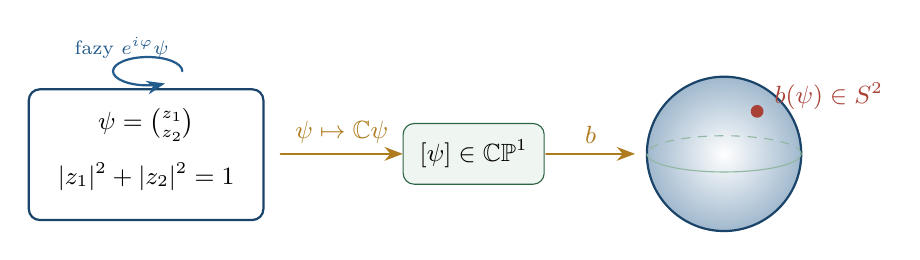
\begin{tikzpicture}[>=Stealth,line cap=round,scale=1.0]
 \draw[manifoldblue!75!black,thick,rounded corners]
 (-5.6,-.72) rectangle (-2.62,.94);
 \node[font=\small] at (-4.11,.49)
   {$\psi=\binom{z_1}{z_2}$};
 \node[font=\small] at (-4.11,-.17)
   {$|z_1|^2+|z_2|^2=1$};
 \draw[->,manifoldblue,thick] (-3.65,1.17)
  arc[start angle=0,end angle=300,x radius=.44,y radius=.18];
 \node[font=\scriptsize,manifoldblue] at (-4.42,1.47)
  {fazy $e^{i\varphi}\psi$};
 \draw[->,thick,manifoldgold!85!black] (-2.4,.12)--(-.85,.12)
  node[midway,above,font=\small] {$\psi\mapsto\C\psi$};
 \node[draw=manifoldgreen!80!black,rounded corners,
  fill=manifoldgreen!8,font=\small,inner sep=6pt] at (.05,.12)
  {$[\psi]\in\mathbb{CP}^1$};
 \draw[->,thick,manifoldgold!85!black] (.97,.12)--(2.1,.12)
  node[midway,above,font=\small] {$b$};
 \shade[inner color=white,outer color=manifoldblue!43] (3.23,.12) circle (.98);
 \draw[manifoldblue!75!black,thick] (3.23,.12) circle (.98);
 \draw[manifoldgreen!55,thin] (2.25,.12)
   arc[start angle=180,end angle=360,x radius=.98,y radius=.23];
 \draw[manifoldgreen!55,thin,dashed] (4.21,.12)
   arc[start angle=0,end angle=180,x radius=.98,y radius=.23];
 \fill[manifoldred] (3.65,.66) circle (2.3pt);
 \node[manifoldred,font=\small] at (4.56,.85) {$b(\psi)\in S^2$};
\end{tikzpicture}
\caption{Spinor jednostkowy $\psi\in\C^2$ ma fazę,
która nie zmienia prostej $[\psi]\in\mathbb{CP}^1$.
Wzór~\eqref{eq:spin-bloch} przypisuje tej prostej
punkt sfery. To łączy spinory z grassmannianem prostych.}
\label{fig:spin-bloch}
\end{figure}

\section{Struktury spinowe i wiązki spinorów}
\label{sec:struktura-spinowa}

Dotąd wektory, obroty i spinory należały do jednej
ustalonej przestrzeni $\R^n$. Na rozmaitości
przestrzeń $T_pM$ zmienia się z $p$.
Gładka rodzina dodatnio określonych iloczynów
skalarnych $g_p$ na $T_pM$ to \emph{metryka
riemannowska}. Pozwala wybierać bazy ortonormalne
w każdym punkcie. Jeśli $M$ jest zorientowana,
możemy wybierać bazy o dodatniej orientacji.

\emph{Wiązka dodatnio zorientowanych ramek
ortonormalnych} $F^+(M)\to M$ ma w punkcie $p$
za włókno wszystkie uporządkowane bazy
$(u_1,\ldots,u_n)$ przestrzeni $T_pM$,
które są ortonormalne i dodatnie.
Grupa $\mathrm{SO}(n)$ działa z prawej strony
przez zmianę takiej bazy. Nie ma wyróżnionej
bazy w każdym włóknie; lokalnie wiązka wygląda
jednak jak $U\times\mathrm{SO}(n)$.
Wiązkę o takiej lokalnej postaci, z wolnym
działaniem grupy przechodzącym tranzytywnie
na każdym włóknie, nazywamy \emph{wiązką główną}.

\begin{definicja}[Struktura spinowa i wiązka spinorów]
\index{struktura spinowa i wiazka spinorow@Struktura spinowa i wiązka spinorów}
\label{def:struktura-spinowa}
Dla zorientowanej rozmaitości riemannowskiej
$M^n$, $n\geq2$, \emph{struktura spinowa}
składa się z wiązki głównej
$P_{\mathrm{Spin}}\to M$ o grupie
$\operatorname{Spin}(n)$ oraz odwzorowania
gładkiego $\lambda:P_{\mathrm{Spin}}\to F^+(M)$
nad identycznością bazy, takiego że
\[
 \lambda(pg)=\lambda(p)\rho(g),
 \qquad g\in\operatorname{Spin}(n),
\]
a $\lambda$ ograniczona do każdego włókna
jest dwukrotnym nakryciem.
\emph{Wiązka spinorów} to wiązka zespolona
\[
 S:=P_{\mathrm{Spin}}\times_{\operatorname{Spin}(n)}\Delta_n.
\]
Jej elementami są klasy par $(p,\psi)$,
$p\in P_{\mathrm{Spin}}$, $\psi\in\Delta_n$,
z relacją $(pg,\psi)\sim(p,c(g)\psi)$.
\emph{Polem spinorowym} nazywamy gładki przekrój $S$.
Tę samą definicję stosujemy do dowolnej zorientowanej wiązki
euklidesowej $E$ rzędu $n$, zastępując $F^+(M)$ wiązką jej
dodatnich ramek ortonormalnych $F^+(E)$.
\end{definicja}

Po wyborze lokalnej ramki spinowej $s_i:U_i\to P_{\mathrm{Spin}}$
wiązka $S$ wygląda jak $U_i\times\Delta_n$. Ustalmy kierunek
zmian: jeśli $s_j=s_i h_{ij}$, to
$[s_j,\psi_j]=[s_i,c(h_{ij})\psi_j]$, zatem współrzędne
tego samego spinora spełniają $\psi_i=c(h_{ij})\psi_j$.
Przy przejściu od kolumny $i$ do kolumny $j$ używamy więc
macierzy odwrotnej. Z równości dla lokalnych ramek wynika też
$h_{ij}h_{jk}=h_{ik}$; reprezentacja $c$ przenosi tę równość
na macierze przejścia, co uzasadnia strukturę wiązki wektorowej $S$.
Zauważmy też, że $\lambda$ jest nakryciem całych przestrzeni:
w lokalnej trywializacji zadanej przez $s_i$ i ramkę $\lambda\circ s_i$
ma postać $(x,g)\mapsto(x,\rho(g))$.
Jeśli zmiana ramki wektorowej wykonuje pełny
obrót o $2\pi$, jej podniesienie w Spin
może dojść do $-1$. Wtedy wektory wracają
do wartości początkowych, lecz spinor dostaje
znak minus. To lokalna treść różnicy między
wiązką wektorów i wiązką spinorów.

\begin{przyklad}[Płaszczyzna i sfera są spinowe]
Na $\R^n$ standardowe ramki dają
$F^+(\R^n)\cong\R^n\times\mathrm{SO}(n)$.
Bierzemy
$P_{\mathrm{Spin}}=\R^n\times\operatorname{Spin}(n)$
i $\lambda(x,s)=(x,\rho(s))$; spinory
tworzą trywialną wiązkę
$S\cong\R^n\times\Delta_n$.

Na sferze $S^2\subset\R^3$ każda dodatnia
ramka styczna $(u,v)$ w punkcie $p$ wyznacza
macierz o kolumnach $(u,v,p)\in\mathrm{SO}(3)$.
To utożsamia $F^+(S^2)$ z $\mathrm{SO}(3)$,
a rzut do bazy wysyła macierz na jej trzecią
kolumnę $p$. Dwukrotne nakrycie
$\mathrm{SU}(2)\cong\operatorname{Spin}(3)
\to\mathrm{SO}(3)$ z
Przykładu~\ref{prz:spin3} daje odwzorowanie $\lambda$.
Rzut z $\operatorname{Spin}(3)$ do sfery ma postać
$q(s)=\rho(s)e_3$. Używamy jednej, ustalonej podgrupy
$H=\rho^{-1}(\operatorname{Stab}(e_3))=\operatorname{Spin}(2)$,
złożonej z $\cos t+\sin t\,e_1e_2$. Działa ona z prawej strony
na $\operatorname{Spin}(3)$ i zachowuje $q(s)$.
Jeśli $q(s)=q(s')$, to $s^{-1}s'\in H$, więc działanie jest
wolne i przechodnie na każdym włóknie. Lokalne gładkie ramki
styczne $(u,v)$ dają lokalne sekcje w $\mathrm{SO}(3)$;
po zmniejszeniu otoczenia podnosimy je przez lokalną odwrotność
nakrycia $\rho$. To zapewnia lokalną trywialność wiązki głównej.
Równość $\lambda(sh)=\lambda(s)\rho(h)$ kończy sprawdzenie
definicji struktury spinowej na sferze.
\end{przyklad}

\begin{uwaga}[Podnoszenie na zbiorze ściągalnym]
\label{rem:spin-podnoszenie}
Użyjemy elementarnego faktu o nakryciach: gładkie odwzorowanie
ze ściągalnego obszaru $U$ do podstawy gładkiego nakrycia ma
gładkie podniesienie po wybraniu obrazu jednego punktu.
Istotnie, drogę od tego punktu podnosimy kolejno przez lokalne
odwrotności nakrycia, dzieląc jej przedział parametrów na skończenie
wiele odcinków. Jednoznaczność na przecięciach daje jednoznaczność
podniesionej drogi. Homotopię dróg o ustalonych końcach podnosimy
analogicznie po podziale kwadratu parametrów na małe prostokąty,
których obrazy leżą w dziedzinach lokalnych odwrotności.
Końcowy punkt podniesienia nie zmienia się w tej homotopii:
poruszałby się ciągle w dyskretnym włóknie. W obszarze ściągalnym
każde dwie drogi o tych samych końcach są tak homotopijne,
więc ich podniesienia wyznaczają tę samą wartość w punkcie końcowym.
Otrzymana funkcja jest lokalnie złożeniem danej funkcji z jedną
lokalną odwrotnością nakrycia, zatem jest gładka.
Ten sam argument działa na dysku z brzegiem.
\end{uwaga}

\begin{przyklad}[Wiązka, której nie da się podnieść]
\label{prz:nie-spin-linia}
Podłoże $S^2\cong\mathbb{CP}^1$ jest spinowe,
ale nie każda \emph{wiązka} nad nim dopuszcza
podniesienie struktury do Spin.
Weźmy zespoloną wiązkę tautologiczną
$\gamma^1_\C$ nad
$\operatorname{Gr}_1(\C^2)=\mathbb{CP}^1$
i potraktujmy jej włókna jako rzeczywiste
zorientowane płaszczyzny wymiaru $2$.
Na mapie $[1:z]$ mamy ramkę zespoloną
$s_0(z)=(1,z)$, a na mapie $[w:1]$,
$w=1/z$, ramkę $s_\infty(w)=(w,1)$.
Na przecięciu
$s_\infty(1/z)=z^{-1}s_0(z)$.
Po unormowaniu ramek, przy $|z|=1$, $z=e^{i\theta}$, unitarny
czynnik przejścia jest więc $e^{-i\theta}$:
jako rzeczywista izometria obraca płaszczyznę
o kąt $-\theta$. Po przejściu
$0\leq\theta\leq2\pi$ daje pętlę
o nieparzystej liczbie pełnych obrotów.
Ta pętla w $\mathrm{SO}(2)$ nie ma
\emph{zamkniętego} podniesienia do $\operatorname{Spin}(2)$:
połowa kąta biegnie
od $0$ do $-\pi$ i kończy w $-1$, nie w $1$.
Gdyby istniała struktura spinowa, ramkę ortonormalną nad każdą
z dwóch półkul można by podnieść do ramki spinowej.
Rzeczywiście, przeciwobraz takiej ramki przez $\lambda$ jest
dwukrotnym nakryciem dysku; Uwagi~\ref{rem:spin-podnoszenie}
używamy do podniesienia identyczności dysku. Przejście między
otrzymanymi ramkami spinowymi na równiku byłoby właśnie
zamkniętym podniesieniem opisanej pętli, co jest sprzecznością.
Zmiana ramki na którejś z dwóch półkul
zmienia pętlę tylko o taką, która przedłuża
się na dysk i ma zerowy całkowity obrót.
Dlatego ten brak podniesienia nie zależy
od wybranych ramek. Wiązka rzeczywista otrzymana przez zapomnienie
struktury zespolonej $\gamma^1_\C$ nie ma struktury
spinowej, mimo że sama sfera $S^2$ ją ma.
\end{przyklad}

\begin{stwierdzenie}[Znaki na potrójnych przecięciach]
\label{prop:w2-znaki}
Niech $E$ będzie zorientowaną wiązką euklidesową
rzędu $n\geq2$ nad $M$. Weźmy dostatecznie drobne
pokrycie trywializujące $(U_i)$, w którym
niepuste skończone przecięcia są ściągalne. Takie pokrycie
nazywamy \emph{dobrym}; w tym stwierdzeniu zakładamy jego wybór.
Niech $g_{ij}:U_i\cap U_j\to\mathrm{SO}(n)$
przepisują współrzędne z trywializacji $j$ do trywializacji $i$,
więc $g_{ij}g_{jk}=g_{ik}$.
Na przecięciach wybierzmy podniesienia
$h_{ij}:U_i\cap U_j\to\operatorname{Spin}(n)$
z $\rho(h_{ij})=g_{ij}$ i $h_{ji}=h_{ij}^{-1}$.
Wtedy na potrójnym przecięciu
\begin{equation}\label{eq:w2-znaki}
 \varepsilon_{ijk}:=h_{ij}h_{jk}h_{ki}
          \in\{1,-1\}.
\end{equation}
Wiązka $E$ ma strukturę spinową dokładnie wtedy,
gdy wybory $h_{ij}$ można zmodyfikować znakami
tak, aby wszystkie $\varepsilon_{ijk}$ wynosiły $1$.
\end{stwierdzenie}
\begin{proof}
Z warunku kocyklu dla $g_{ij}$ mamy
$\rho(\varepsilon_{ijk})
=g_{ij}g_{jk}g_{ki}=I$.
Twierdzenie~\ref{thm:spin-nakrycie} mówi, że
jądro $\rho$ to $\{\pm1\}$; ponieważ znak jest
dyskretny, $\varepsilon_{ijk}$ jest lokalnie stały.
Nie ma problemu z samym podniesieniem
$g_{ij}$ na ściągalnym przecięciu:
zapewnia je Uwaga~\ref{rem:spin-podnoszenie}.
Przyjmujemy też $h_{ii}=1$.

Jeżeli na każdym potrójnym przecięciu
$\varepsilon_{ijk}=1$, to
$h_{ij}h_{jk}=h_{ik}$.
Są to funkcje przejścia z warunkiem kocyklu.
Sklejamy $U_i\times\operatorname{Spin}(n)$ relacją
$(x,a)_j\sim(x,h_{ij}(x)a)_i$. Warunek kocyklu zapewnia
przechodniość tej relacji, a gładkie przejścia zapewniają lokalne
trywializacje, jak w Sekcji~\ref{sec:wiazki-wektorowe}.
Działanie z prawej strony jest dobrze określone, wolne
i przechodnie we włóknach, więc otrzymujemy wiązkę główną.
Jeśli $f_i$ oznacza wybraną lokalną ramkę $E$, to
$\lambda([x,a]_i)=f_i(x)\rho(a)$ jest niezależne od reprezentanta,
ponieważ $f_j=f_i g_{ij}$ i $\rho(h_{ij})=g_{ij}$.
Lokalnie jest to $\id\times\rho$, a więc spełnia definicję
struktury spinowej.
Odwrotnie, w istniejącej strukturze spinowej podnosimy każdą
ustaloną ramkę $f_i$ do ramki spinowej nad ściągalnym $U_i$.
Stosujemy Uwagę~\ref{rem:spin-podnoszenie} do dwukrotnego
nakrycia będącego przeciwobrazem $f_i$ przez $\lambda$.
Przejścia tych ramek podnoszą właśnie dane $g_{ij}$ i spełniają
warunek kocyklu, więc wszystkie znaki są $1$.
Dowolne dwa odwzorowania $h_{ij}$ nad
tym samym $g_{ij}$ różnią się na spójnym
przecięciu stałym znakiem
$\delta_{ij}\in\{\pm1\}$.
Zmiana podniesień zastępuje
$\varepsilon_{ijk}$ przez
$\delta_{ij}\delta_{jk}\delta_{ki}
\varepsilon_{ijk}$, co dowodzi
sformułowania o modyfikacji znakami.
\end{proof}

\begin{uwaga}[Druga klasa Stiefela--Whitneya]
Zdarza się, że pojedynczych znaków
$\varepsilon_{ijk}$ nie da się wszystkich
usunąć. Ich układ spełnia warunek zgodności
na poczwórnych przecięciach: dwa sposoby
pomnożenia $h_{ij}h_{jk}h_{k\ell}$
dają
$\varepsilon_{ijk}\varepsilon_{ik\ell}
=\varepsilon_{jk\ell}\varepsilon_{ij\ell}$.
Taką rodzinę znaków nazywamy
\emph{dwukocyklowym} zapisem przeszkody.
Zmiany przez $\delta_{ij}$ z dowodu
uznajemy za równoważne. Nie zmienia tego wybór lokalnych ramek:
jeśli $f'_i=f_i a_i$, wybieramy podniesienia $b_i$ funkcji $a_i$
nad ściągalnymi $U_i$. Wtedy $g'_{ij}=a_i^{-1}g_{ij}a_j$
mają podniesienia $h'_{ij}=b_i^{-1}h_{ij}b_j$.
Ich iloczyn na potrójnym przecięciu to
$b_i^{-1}\varepsilon_{ijk}b_i=\varepsilon_{ijk}$,
bo znaki należą do centrum grupy Spin.
Klasa tego układu w
$H^2(M;\Z/2)$ nazywa się
\emph{drugą klasą Stiefela--Whitneya}
$w_2(E)$. Na dobrym pokryciu
$w_2(E)=0$ oznacza dokładnie, że znaki
można usunąć, czyli że struktura spinowa
istnieje. Identyfikacja klas z różnych
pokryć to twierdzenie kohomologii Čech;
używamy tu tylko elementarnego testu
podnoszenia funkcji przejścia dowiedzionego
wyżej. Dla wiązki w
Przykładzie~\ref{prz:nie-spin-linia}
przeszkoda jest niezerowa.
\end{uwaga}

\par\smallskip
{\footnotesize\noindent\emph{Dalsza lektura:}
Rachunki z konwencją $v^2=-\|v\|^2$
można porównać z notatkami Briana Conrada,
\emph{Clifford algebras and spin groups},
\url{https://math.stanford.edu/~conrad/210CPage/handouts/clifford.pdf}.
Budowę struktur spinowych i opis przeszkody
$w_2$ rozwijają notatki Konstantina Wernliego,
\emph{Lecture Notes on Spin Geometry},
\url{https://arxiv.org/pdf/1911.09766}.
Obie lektury używają miejscami innej kolejności tematów.
Powyższy test znaków został dowiedziony bez użycia kohomologii;
jego interpretacja jako klasy w $H^2$ korzysta z teorii
kohomologii Čech, której tutaj nie dowodziliśmy.\par}
\clearpage

\chapter{Podstawy algebry abstrakcyjnej}
\label{ch:algebra-abstrakcyjna}
\index{algebra abstrakcyjna@Algebra abstrakcyjna}

Zbierzemy pojęcia grup, pierścieni i modułów potrzebne
do algebry homologicznej. Konstrukcje ilorazowe pozwalają
narzucać relacje, a iloczyn tensorowy pozwala zastąpić
odwzorowanie dwuliniowe liniowym. Wcześniejszy
Rozdział~\ref{ch:algebra-tensorowa} dotyczył przestrzeni
nad ciałem; tutaj pracujemy nad pierścieniem.
W Rozdziale~\ref{ch:grass-spin} wystąpił też moduł
algebry Clifforda; wrócimy do tego przykładu.

\section{Grupy, słowa i prezentacje}
\label{sec:grupy-prezentacje-5}
\index{grupa wolna@Grupa wolna}
\index{prezentacja grupy@Prezentacja grupy}

Zanim przejdziemy do modułów, zbierzmy język
potrzebny przy grupie podstawowej i
Twierdzeniu~\ref{thm:van-kampen}. Grupa opisuje
odwracalne składanie działań. W grupie klas
pętli opartych w jednym punkcie działaniem
jest składanie pętli, a odwrotność reprezentuje
pętla przebiegnięta w przeciwnym kierunku.

\subsection*{Grupy, homomorfizmy i ilorazy}

\begin{definicja}[Grupa i homomorfizm]
\index{grupa i homomorfizm@Grupa i homomorfizm}
\label{def:grupa-hom-5}
\emph{Grupa} $(G,\cdot,1)$ to zbiór z łącznym
mnożeniem, elementem neutralnym $1$ i
odwrotnością $g^{-1}$ każdego $g\in G$.
Nie zakładamy przemienności. Odwzorowanie
$\varphi:G\to H$ jest \emph{homomorfizmem},
jeśli $\varphi(gh)=\varphi(g)\varphi(h)$.
Wtedy $\varphi(1)=1$ i
$\varphi(g^{-1})=\varphi(g)^{-1}$.
Istotnie, $\varphi(1)^2=\varphi(1)$, więc skracanie daje
$\varphi(1)=1$; następnie stosujemy $\varphi$ do $gg^{-1}=1$.
Bijektywny homomorfizm nazywamy \emph{izomorfizmem}.
\end{definicja}

Przykładem jest $(\Z,+,0)$;
w zapisie addytywnym odwrotnością $m$
jest $-m$. Grupa permutacji trzech
elementów dostarcza przykładu
nieprzemiennego: przestawienia
$(12)(23)$ i $(23)(12)$ są różne.

\begin{definicja}[Podgrupa normalna i iloraz]
\index{podgrupa normalna i iloraz@Podgrupa normalna i iloraz}
\label{def:normal-quotient-5}
\emph{Podgrupa} $N\leq G$ to podzbiór zawierający $1$
i zamknięty na mnożenie oraz branie odwrotności.
\emph{Warstwa lewostronna} to $gN=\{gn:n\in N\}$.
Mamy $gN=hN$ dokładnie wtedy, gdy $h^{-1}g\in N$:
z równości warstw wynika $g=hn$ dla pewnego $n\in N$,
a z $g=hn$ wynika $gN=hnN=hN$.
Podgrupa $N\leq G$ jest \emph{normalna},
gdy $gNg^{-1}=N$ dla każdego $g\in G$.
Wówczas zbiór warstw $G/N$ staje się
grupą przez $(gN)(hN)=ghN$.
Jądro homomorfizmu
$\ker\varphi=\{g:\varphi(g)=1\}$
jest normalne. \emph{Domknięcie normalne}
zbioru $R\subset G$, oznaczane
$\langle\!\langle R\rangle\!\rangle$,
jest najmniejszą podgrupą normalną
zawierającą $R$.
\end{definicja}

\begin{proof}[Dlaczego iloraz jest dobrze określony?]
Jeśli $g'=gn$ i $h'=hm$ dla $n,m\in N$,
to $g'h'=gnhm=gh(h^{-1}nh)m$.
Normalność daje $h^{-1}nh\in N$,
zatem $g'h'N=ghN$. Mnożenie
nie zależy więc od wybranych
reprezentantów. Łączność dziedziczymy z $G$;
elementem neutralnym jest $N$, a odwrotnością $gN$ jest $g^{-1}N$.
Dla jądra:
$\varphi(gng^{-1})=
\varphi(g)1\varphi(g)^{-1}=1$.
Elementy domknięcia normalnego
są skończonymi iloczynami
sprzężeń $grg^{-1}$ i ich
odwrotności, $r\in R$:
zbiór tych iloczynów jest
podgrupą normalną zawierającą
$R$ i mieści się w każdej takiej
podgrupie.
\end{proof}

\begin{przyklad}[Reszty modulo $m$]
\label{prz:Zmodm-grupa-5}
Niech $m\geq2$.
W grupie addytywnej $\Z$ każda
podgrupa jest normalna.
Iloraz $\Z/m\Z$ ma elementy
$[0],\ldots,[m-1]$ i dodawanie
$[a]+[b]=[a+b]$. Homomorfizm
$\Z\to\Z/m\Z$ ma jądro $m\Z$.
\end{przyklad}

\subsection*{Grupy wolne i iloczyn wolny}

\begin{definicja}[Grupa wolna i iloczyn wolny]
\index{grupa wolna i iloczyn wolny@Grupa wolna i iloczyn wolny}
\index{slowo w grupie wolnej@słowo w grupie wolnej}
\label{def:free-groups-5}
Niech $A$ będzie zbiorem \emph{symboli},
zwanych generatorami. Dla każdego $a\in A$
tworzymy nowy symbol $a^{-1}$;
zbiór tych nowych symboli oznaczamy $A^{-1}$
i przyjmujemy $(a^{-1})^{-1}=a$.
\emph{Słowo} w alfabecie
$A^{\pm1}=A\sqcup A^{-1}$ jest skończonym
ciągiem liter $x_1\cdots x_r$, $r\geq0$.
Długość słowa to $r$; jedyne słowo długości
zero oznaczamy $\varnothing$ i nazywamy pustym.
Słowa można sklejać, czyli konkatenować:
$(x_1\cdots x_r)(y_1\cdots y_s)
=x_1\cdots x_ry_1\cdots y_s$.

\emph{Redukcja elementarna} usuwa sąsiednie
litery $xx^{-1}$ lub $x^{-1}x$.
Słowo jest \emph{zredukowane}, gdy nie zawiera
takiej pary. Dwa słowa uznajemy za równoważne,
jeżeli można przejść od jednego do drugiego
skończonym ciągiem wstawień lub usunięć
takich par. \emph{Grupa wolna} $F(A)$
to zbiór tych klas, z mnożeniem zadanym
przez sklejanie słów.

Dla grup $G,H$ \emph{iloczyn wolny} $G*H$
powstaje ze słów w \emph{rozłącznej sumie} alfabetów
$(G\setminus\{1_G\})\sqcup(H\setminus\{1_H\})$.
Litera pamięta swój czynnik, nawet gdy $G=H$.
Redukcja zastępuje sąsiednie litery jednego czynnika
ich iloczynem w tym czynniku; jeśli iloczyn jest jedynką,
usuwa obie litery. Równoważność słów dopuszcza zarówno
te redukcje, jak i operacje odwrotne.
$G*H$ jest zbiorem klas z mnożeniem przez konkatenację.
Słowo zredukowane ma litery z obu czynników naprzemiennie.
\end{definicja}

Zanim utożsamimy klasy ze słowami zredukowanymi,
trzeba wiedzieć, że wynik redukcji nie zależy
od kolejności kasowania par. Sam zbiór
\emph{wszystkich} słów z konkatenacją
jest tylko monoidem: słowa $aa^{-1}$
i $\varnothing$ nie są w nim dosłownie równe.

\begin{stwierdzenie}[Jednoznaczna postać zredukowana]
\index{redukcja slowa@redukcja słowa}
\label{prop:free-reduction-5}
Każda klasa w $F(A)$ zawiera dokładnie jedno
słowo zredukowane. Jeżeli $\operatorname{red}(w)$
oznacza to słowo, działanie grupowe ma postać
\[
 u\cdot v=\operatorname{red}(uv),\qquad
 1=\varnothing,\qquad
 (x_1\cdots x_r)^{-1}=x_r^{-1}\cdots x_1^{-1}.
\]
\end{stwierdzenie}
\begin{proof}
Czytamy słowo od lewej do prawej i trzymamy
\emph{stos} już przeczytanych liter.
Gdy następna litera jest odwrotnością
litery na wierzchu stosu, zdejmujemy wierzch;
w przeciwnym razie dokładamy nową literę.
Po ostatnim kroku na stosie nie ma sąsiedniej
pary odwrotnej, więc otrzymaliśmy słowo
zredukowane. Po każdym kroku stos reprezentuje tę samą
klasę co przeczytany fragment: dopisujemy literę albo
usuwamy końcową parę odwrotną. Wynik należy więc do klasy
początkowego słowa.

Sprawdźmy niezależność od usuwania par.
Operacja dopisania litery $x$ do słowa
na stosie jest odwracalna: operacja
dopisania $x^{-1}$ cofa ją, zarówno gdy
pierwszy krok dołożył literę, jak i wtedy,
gdy ją skasował. Dlatego przeczytanie
fragmentu $xx^{-1}$ nie zmienia stanu stosu.
Usunięcie takiego fragmentu z dowolnego miejsca
słowa nie zmienia końcowego wyniku algorytmu.
Każde słowo równoważne daje zatem ten sam wynik.
Jeśli słowo jest już zredukowane, algorytm
pozostawia je bez zmian; w każdej klasie
może więc być tylko jedno takie słowo.

Sklejanie jest łączne przed redukcją, a
usuwanie par nie zmienia wyniku algorytmu.
Stąd $\operatorname{red}(\operatorname{red}(uv)w)
=\operatorname{red}(uvw)
=\operatorname{red}(u\operatorname{red}(vw))$.
Słowo puste jest jedynką. Zapisane w tezie
słowo odwrotne po sklejeniu z oryginałem
redukuje się kolejno od środka do słowa pustego.
To sprawdza wszystkie aksjomaty grupy.
\end{proof}

\begin{przyklad}[Słowa i działanie na słowach]
\label{prz:redukcja-slow-5}
W $F(\{a,b\})$ słowo
$ab\,b^{-1}a^{-1}ba$
redukujemy najpierw do
$aa^{-1}ba$, a następnie
do $ba$. Słowa $ab$ i $ba$
są już zredukowane i różne,
więc grupa ta nie jest przemienna.
Dla jednego generatora każde słowo
redukuje się do $a^m$ z jednoznacznym
$m\in\Z$; stąd $F(\{a\})\cong\Z$.

Grupa $F(A)$ działa na zbiorze zredukowanych
słów przez mnożenie z lewej:
$u\cdot w=\operatorname{red}(uw)$.
Na przykład $a\cdot(a^{-1}b)=b$.
Jest to działanie, bo łączność udowodniono
powyżej; odwrotna operacja do działania
przez $a$ to działanie przez $a^{-1}$.
Jest ono przechodnie, gdyż $w\cdot\varnothing=w$,
i wolne: jeśli $u\cdot w=w$, to w grupie
$uw=w$, zatem po pomnożeniu przez $w^{-1}$
dostajemy $u=1$. Ten sam zbiór ma również
działanie z prawej $w\cdot u=\operatorname{red}(wu)$.
Rysunek~\ref{fig:free-words-5} pokazuje
pojedyncze kroki tego drugiego działania.
Na przykład iloczyn dwóch zredukowanych słów
$ab$ i $b^{-1}a$ trzeba jeszcze skrócić:
$\operatorname{red}(ab\,b^{-1}a)=a^2$.
\end{przyklad}

\begin{figure}[htbp]
\centering
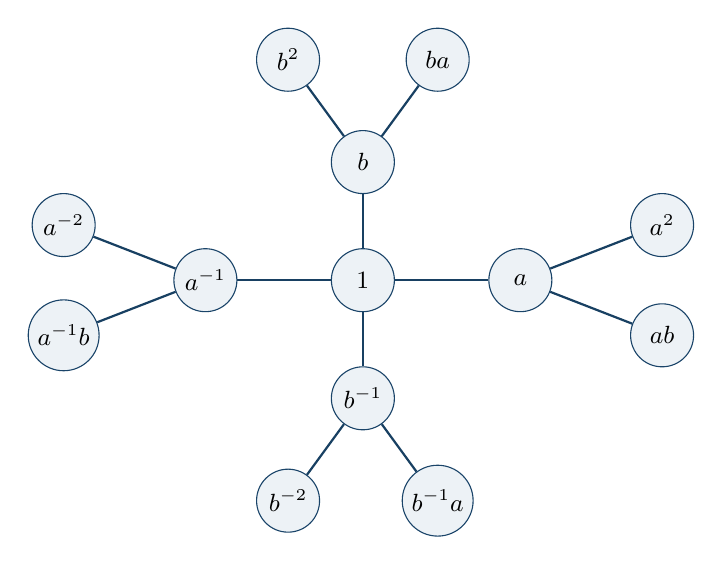
\begin{tikzpicture}[>=Latex,font=\small,
 every node/.style={circle,draw=manifoldblue!75!black,
 fill=manifoldblue!8,inner sep=2pt,minimum size=8mm}]
 \node (e) at (0,0) {$1$};
 \node (a) at (2,0) {$a$};
 \node (ai) at (-2,0) {$a^{-1}$};
 \node (b) at (0,1.5) {$b$};
 \node (bi) at (0,-1.5) {$b^{-1}$};
 \node (aa) at (3.8,.7) {$a^2$};
 \node (ab) at (3.8,-.7) {$ab$};
 \node (aiai) at (-3.8,.7) {$a^{-2}$};
 \node (aib) at (-3.8,-.7) {$a^{-1}b$};
 \node (bb) at (-.95,2.8) {$b^2$};
 \node (ba) at (.95,2.8) {$ba$};
 \node (bibi) at (-.95,-2.8) {$b^{-2}$};
 \node (bia) at (.95,-2.8) {$b^{-1}a$};
 \foreach \x/\y in {e/a,e/ai,e/b,e/bi,a/aa,a/ab,
 ai/aiai,ai/aib,b/bb,b/ba,bi/bibi,bi/bia}
   \draw[thick,manifoldblue!70!black] (\x)--(\y);
\end{tikzpicture}
\caption{Fragment grafu słów zredukowanych w
$F(\{a,b\})$. Krawędź oznacza dopisanie
z prawej jednej litery $a^{\pm1}$ albo $b^{\pm1}$
i ewentualną redukcję. Powrót po krawędzi
odpowiada dopisaniu litery odwrotnej.}
\label{fig:free-words-5}
\end{figure}

\begin{stwierdzenie}[Własność uniwersalna grupy wolnej]
\label{prop:free-universal-5}
Dla dowolnej grupy $K$ i dowolnego wyboru
elementów $h_a\in K$, $a\in A$, istnieje
dokładnie jeden homomorfizm $\Phi:F(A)\to K$
spełniający $\Phi(a)=h_a$.
\end{stwierdzenie}
\begin{proof}
Na słowach musi on mieć postać
\[
 \Phi(a_1^{\epsilon_1}\cdots a_r^{\epsilon_r})
 =h_{a_1}^{\epsilon_1}\cdots h_{a_r}^{\epsilon_r},
 \qquad \epsilon_i\in\{1,-1\}.
\]
Usunięcie sąsiedniej pary odwrotnej nie zmienia
iloczynu po prawej. Wzór zależy więc tylko
od klasy słowa i jest dobrze określony.
Sklejanie słów odpowiada mnożeniu obrazów,
zatem $\Phi$ jest homomorfizmem.
Każde słowo jest iloczynem generatorów
i ich odwrotności, co dowodzi jednoznaczności.
Właśnie brak dodatkowych relacji między
generatorami nazywamy \emph{wolnością}.
\end{proof}

\begin{stwierdzenie}[Postać normalna i własność uniwersalna iloczynu wolnego]
\label{prop:free-product-normal-5}
Każdy element $G*H$ ma dokładnie jeden zapis jako słowo
naprzemienne o literach różnych od jedynki, z dopuszczeniem
słowa pustego. Odwzorowania $G\to G*H$ i $H\to G*H$,
wysyłające element niejednostkowy na słowo jednoliterowe,
a jedynkę na słowo puste, są iniektywnymi homomorfizmami.
Dla każdej pary homomorfizmów $f:G\to K$, $h:H\to K$
istnieje dokładnie jeden homomorfizm $\Phi:G*H\to K$
ograniczający się na czynnikach do $f$ oraz $h$.
\end{stwierdzenie}
\begin{proof}
Czytamy litery po kolei i przechowujemy stos liter
niejednostkowych, pochodzących naprzemiennie z obu czynników.
Dla $x$ z jednego czynnika oznaczmy przez $T_x$ operację
dopisania $x$: literę z innego czynnika dokładamy, a z tego
samego mnożymy z ostatnią literą stosu. Gdy iloczyn jest
jedynką, zdejmujemy tę ostatnią literę. Przyjmujemy $T_1=\id$.
Każdy krok jest dozwoloną redukcją, więc wynik algorytmu
należy do klasy czytanego słowa.

Kluczowa jest równość $T_y(T_x(u))=T_{xy}(u)$, gdy $x,y$
pochodzą z tego samego czynnika. Jeśli któraś litera jest
jedynką, równość jest natychmiastowa. W pozostałym przypadku:
\begin{itemize}[leftmargin=*]
\item Gdy $u$ jest pusty albo kończy się literą drugiego
czynnika, najpierw dopisujemy $x$, potem zastępujemy $xy$
jedną literą albo usuwamy je, jeśli $xy=1$. To właśnie $T_{xy}(u)$.
\item Gdy $u=vz$ i $z$ jest z tego samego czynnika co $x,y$,
słowo $v$ jest puste albo kończy się w drugim czynniku.
Jeśli $zx\ne1$, dwa kroki zastępują końcówkę przez
$(zx)y=z(xy)$, z usunięciem jedynki. Dla $xy=1$ odzyskujemy $vz$;
dla $xy\ne1$ jest to pojedynczy krok $T_{xy}$.
Jeśli $zx=1$, pierwszy krok usuwa $z$, a drugi daje $vy$.
Z kolei $z(xy)=y$; gdy $xy\ne1$, pojedynczy krok również daje $vy$.
Gdy $xy=1$, mamy $y=z$, więc $vy=u=T_1(u)$.
\end{itemize}
Zastąpienie sąsiednich liter ich iloczynem nie zmienia zatem
stosu po przeczytaniu tego fragmentu, ani wyniku po przeczytaniu
reszty słowa. Dotyczy to także odwrotnej operacji.
Wynik jest stały na klasie równoważności. Ponieważ algorytm
pozostawia słowo naprzemienne bez zmian, w każdej klasie jest
dokładnie jedno takie słowo.

Relacje można wykonywać wewnątrz dowolnego dłuższego słowa,
więc konkatenacja jest dobrze określona na klasach i łączna.
Słowo puste jest jedynką, a odwrócenie kolejności liter
i zastąpienie ich odwrotnościami daje odwrotność słowa.
Relacje wewnątrz czynników zapewniają, że ich odwzorowania
do $G*H$ są homomorfizmami. Jednoznaczność postaci normalnej
daje ich iniektywność; obrazy czynników mają tylko jedynkę wspólną.

Definiujemy $\Phi(x_1\cdots x_r)$ jako iloczyn obrazów liter,
używając $f$ lub $h$ zależnie od czynnika.
Redukcja w jednym czynniku nie zmienia tego iloczynu, bo
$f$ i $h$ są homomorfizmami. Wzór przechodzi więc na klasy.
Konkatenacja słów odpowiada mnożeniu obrazów, a każdy element
jest iloczynem liter z czynników; daje to istnienie i jednoznaczność $\Phi$.
\end{proof}

Ta własność uniwersalna będzie używana w
Twierdzeniu~\ref{thm:van-kampen}.

Na przykład dla $G=\langle a\rangle\cong\Z$
i $H=\langle b\rangle\cong\Z$ własności
uniwersalne dają $G*H\cong F(\{a,b\})$.
Iloczyn słów naprzemiennych
$(ab)(b^{-1}a)$ redukuje się do $a^2$:
po skasowaniu $bb^{-1}$ zostaje $aa$.

Nie należy mylić iloczynu wolnego z iloczynem prostym.
Dla $G=\langle a\mid a^2=1\rangle$ i
$H=\langle b\mid b^2=1\rangle$, obu rzędu dwa,
słowa $(ab)^k$, $k\geq0$, są różnymi postaciami normalnymi.
Zatem $G*H$ jest nieskończony, podczas gdy $G\times H$ ma
cztery elementy. W $G*H$ nie narzucamy przemienności liter
z różnych czynników.

\subsection*{Generatory i relacje}

\begin{definicja}[Prezentacja grupy]
\index{prezentacja grupy@Prezentacja grupy}
\label{def:prezentacja-grupy-5}
Jeśli $R$ jest zbiorem słów
w $F(A)$, to
\[
 \langle A\mid R\rangle
 :=F(A)/\langle\!\langle R\rangle\!\rangle
\]
nazywamy \emph{grupą o generatorach}
$A$ i \emph{relacjach} $R$.
Relacja $r=1$ oznacza, że jej
wszystkie konsekwencje po
mnożeniu i sprzęganiu również
stają się jedynką.
\end{definicja}

\begin{przyklad}[Prezentacja grupy torusa]
\label{prz:prezentacja-torusa-5}
Niech $F(a,b)$ będzie grupą wolną
na dwóch symbolach. Relacja
$aba^{-1}b^{-1}=1$
jest równoważna $ab=ba$.
Po jej narzuceniu każde słowo
można przestawić do postaci
$a^m b^n$, $m,n\in\Z$.
Odwzorowanie
$F(a,b)\to\Z^2$ dane przez
$a\mapsto(1,0)$,
$b\mapsto(0,1)$
zabija tę relację i wysyła
$a^m b^n$ na $(m,n)$.
Postacie te są więc wzajemnie
różne, a zatem
\[
 \langle a,b\mid aba^{-1}b^{-1}\rangle
 \cong\Z^2.
\]
Sklejenie przeciwnych boków kwadratu
tworzy torus. Brzeg kwadratu przed
sklejeniem odczytujemy jako słowo
$aba^{-1}b^{-1}$.
Topologiczne uzasadnienie, że
prezentacja opisuje $\pi_1(T^2)$,
podamy przy
Twierdzeniu~\ref{thm:van-kampen}.
\end{przyklad}


\subsection*{Iloczyn prosty grup}
\label{subsec:iloczyn-prosty}
\index{iloczyn prosty grup}
\index{grupa!iloczyn prosty}

Iloczyn prosty opisuje niezależne wykonywanie dwóch działań.
\begin{definicja}[Iloczyn prosty]
Dla grup $G,H$ ich \emph{iloczyn prosty} jest zbiorem $G\times H$
z mnożeniem $(g_1,h_1)(g_2,h_2)=(g_1g_2,h_1h_2)$.
Jedynką jest $(e_G,e_H)$, a $(g,h)^{-1}=(g^{-1},h^{-1})$.
Łączność wynika z łączności w każdej współrzędnej.
\end{definicja}

Inkluzje $g\mapsto(g,e_H)$ i $h\mapsto(e_G,h)$ są homomorfizmami.
Ich obrazy są normalne: sprzęganie odbywa się współrzędnie.
Elementy z różnych czynników komutują i każdy element ma jednoznaczny
rozkład $(g,h)=(g,e_H)(e_G,h)$.

\begin{stwierdzenie}[Wewnętrzny iloczyn prosty]
Jeśli $G,H$ są normalnymi podgrupami $K$, $G\cap H=\{e\}$ i $K=GH$,
to $F:G\times H\to K$, $F(g,h)=gh$, jest izomorfizmem.
Zapis $GH$ oznacza zbiór wszystkich iloczynów $gh$.
\end{stwierdzenie}
\begin{proof}
Komutator $ghg^{-1}h^{-1}$ należy do $G$ i do $H$ przez normalność,
więc jest jedynką. Dlatego $gh=hg$ i
\[
 F(g_1g_2,h_1h_2)=g_1g_2h_1h_2=g_1h_1g_2h_2
 =F(g_1,h_1)F(g_2,h_2).
\]
Warunek $K=GH$ daje surjektywność. Jeśli $F(g,h)=e$, to
$g=h^{-1}\in G\cap H$, zatem $g=h=e$; jądro jest trywialne.
\end{proof}

\begin{przyklad}[Grupy cykliczne i grupa Kleina]
Grupę generowaną przez jeden element nazywamy \emph{cykliczną}.
Piszemy $C_m=\Z/m\Z$ dla $m\geq1$. Rząd elementu jest najmniejszą
dodatnią liczbą potęg dającą jedynkę, o ile taka liczba istnieje.
W $C_m\times C_n$ element $([1],[1])$ ma rząd
$\operatorname{lcm}(m,n)$: jego $j$-krotność znika dokładnie wtedy,
gdy $m\mid j$ i $n\mid j$. Dla $\gcd(m,n)=1$ rząd wynosi $mn$,
więc ten element generuje całą grupę i $C_m\times C_n\cong C_{mn}$.
Na przykład $C_2\times C_3\cong C_6$. Natomiast w
$V_4:=C_2\times C_2$, zwanej \emph{grupą Kleina}, każdy niezerowy
element ma rząd dwa, więc nie ma generatora całej czteroelementowej grupy.
\end{przyklad}

\subsection*{Iloczyn półprosty grup}
\label{subsec:iloczyn-polprosty}
\index{iloczyn półprosty grup}
\index{grupa!iloczyn półprosty}
\index{działanie grupy!przez automorfizmy}

Teraz jedna grupa może zmieniać sposób działania drugiej.
\emph{Automorfizmem} grupy $N$ nazywamy izomorfizm $N\to N$;
ich grupa ze składaniem to $\operatorname{Aut}(N)$.
Działanie $H$ na $N$ przez automorfizmy jest homomorfizmem
$\varphi:H\to\operatorname{Aut}(N)$, a więc
$\varphi(h_1h_2)=\varphi(h_1)\circ\varphi(h_2)$.

\begin{definicja}[Iloczyn półprosty]
\emph{Iloczyn półprosty} $N\rtimes_\varphi H$ ma zbiór elementów
$N\times H$ i mnożenie
\[
 (n_1,h_1)(n_2,h_2)
 =\bigl(n_1\varphi(h_1)(n_2),h_1h_2\bigr).
\]
Gdy działanie jest ustalone, skracamy zapis do $N\rtimes H$.
\end{definicja}

Sprawdźmy łączność. Pierwsza współrzędna obu sposobów mnożenia
trzech elementów jest równa
\[
 n_1\varphi(h_1)(n_2)\varphi(h_1h_2)(n_3)
 =n_1\varphi(h_1)\bigl(n_2\varphi(h_2)(n_3)\bigr).
\]
Druga to $h_1h_2h_3$. Jedynką jest $(e_N,e_H)$, a
\[
 (n,h)^{-1}=\bigl(\varphi(h^{-1})(n^{-1}),h^{-1}\bigr);
\]
wstawienie tego wzoru po obu stronach daje jedynkę.
Inkluzje $n\mapsto(n,e_H)$ i $h\mapsto(e_N,h)$ są homomorfizmami.
Pierwszy obraz jest normalny jako jądro homomorfizmu
$(n,h)\mapsto h$. Drugi nie musi być normalny, a wzór
\[
 (e_N,h)(n,e_H)(e_N,h)^{-1}=(\varphi(h)(n),e_H)
\]
pokazuje, że zadane działanie realizuje się przez sprzężenie.
Dla działania trywialnego, $\varphi(h)=\id_N$, odzyskujemy iloczyn prosty.

\begin{stwierdzenie}[Wewnętrzny iloczyn półprosty]
\index{iloczyn półprosty grup!wewnętrzny}
Niech $N,H\leq G$, $N\trianglelefteq G$, $N\cap H=\{e\}$ i $G=NH$.
Wtedy $G\cong N\rtimes H$, z działaniem $\varphi(h)(n)=hnh^{-1}$.
\end{stwierdzenie}
\begin{proof}
Normalność zapewnia, że sprzężenie przez $h$ jest automorfizmem $N$,
a składanie sprzężeń daje homomorfizm $\varphi$.
Dla $F(n,h)=nh$ mamy
\[
 F\bigl(n_1(h_1n_2h_1^{-1}),h_1h_2\bigr)
 =n_1h_1n_2h_2=F(n_1,h_1)F(n_2,h_2).
\]
Surjektywność wynika z $G=NH$, a $nh=e$ wymusza
$n=h^{-1}\in N\cap H=\{e\}$, więc $F$ jest iniektywny.
\end{proof}

\begin{uwaga}[Rozszczepiony ciąg dokładny]
\index{ciąg dokładny!rozszczepiony}
\index{rozszerzenie grup!rozszczepione}
Zapis $1\to N\xrightarrow{i}G\xrightarrow{p}H\to1$ oznacza,
że $i$ jest iniekcją, $p$ surjekcją i $i(N)=\ker p$; to
\emph{krótki ciąg dokładny grup}, czyli rozszerzenie $H$ przez $N$.
Jest \emph{rozszczepiony}, gdy istnieje homomorfizm $s:H\to G$
z $p\circ s=\id_H$. Dla iloczynu półprostego są to
$i(n)=(n,e_H)$, $p(n,h)=h$ i $s(h)=(e_N,h)$.
Odwrotnie, w rozszczepionym ciągu $s$ jest iniektywny,
$i(N)\cap s(H)=\{e\}$ i każdy $g\in G$ ma rozkład
$g=(g\,s(p(g))^{-1})s(p(g))$, z pierwszym czynnikiem w $\ker p$.
Poprzednie stwierdzenie daje zatem $G\cong N\rtimes H$.
\end{uwaga}

\begin{przyklad}[Grupa diedralna]
\index{grupa diedralna!jako iloczyn półprosty}
Dla $n\geq3$ niech $r$ będzie obrotem foremnego $n$-kąta o $2\pi/n$,
a $s$ jego odbiciem. Mamy $r^n=s^2=e$ i $srs^{-1}=r^{-1}$.
Każda symetria ma postać $r^j$ lub $r^js$, $0\leq j<n$:
jej obraz jednego wierzchołka i wybór kierunku do sąsiedniego
wyznaczają całą symetrię. Te $2n$ możliwości są różne.
Grupa symetrii $D_n$ jest więc $C_n\rtimes C_2$, gdzie nietrywialny
element $C_2$ odwraca generator $C_n$. Dla trójkąta wszystkie
permutacje trzech wierzchołków są symetriami, stąd
$S_3\cong C_3\rtimes C_2$.
\end{przyklad}

\begin{przyklad}[Grupa afiniczna]
\index{grupa afiniczna!jako iloczyn półprosty}
Grupa odwracalnych macierzy rzeczywistych $\mathrm{GL}(n,\R)$
działa na addytywnej grupie $\R^n$ przez $A\cdot v=Av$.
Grupa odwracalnych odwzorowań afinicznych $x\mapsto Ax+v$ to
$\operatorname{Aff}(n)=\R^n\rtimes\mathrm{GL}(n,\R)$, ponieważ
\[
 A(Bx+w)+v=ABx+(v+Aw),\qquad
 (v,A)(w,B)=(v+Aw,AB).
\]
Macierz i przesunięcie są jednoznaczne: $v$ jest obrazem zera,
a $A$ jest częścią liniową. Czynnik $Aw$ odróżnia ten iloczyn
od iloczynu prostego.
\end{przyklad}

\begin{przyklad}[Ruchy euklidesowe]
\index{grupa euklidesowa!jako iloczyn półprosty}
\index{grupa ruchów euklidesowych}
Niech $\mathrm O(n)=\{A:A^TA=I\}$ i
$\mathrm{SO}(n)=\{A\in\mathrm O(n):\det A=1\}$.
Grupa izometrii przestrzeni euklidesowej to
$E(n)=\R^n\rtimes\mathrm O(n)$, z tym samym prawem składania.
Istotnie, dla izometrii $f$ połóżmy $v=f(0)$ i $g(x)=f(x)-v$.
Tożsamość polaryzacyjna i zachowanie odległości dają
$\langle g(x),g(y)\rangle=\langle x,y\rangle$.
Wektory $g(e_i)$ tworzą bazę ortonormalną, a współrzędne $g(x)$
w tej bazie wynoszą $\langle g(x),g(e_i)\rangle=x_i$.
Zatem $g(x)=\sum_i x_i g(e_i)=Ax$ z $A\in\mathrm O(n)$.
Odwrotnie, każde $Ax+v$ z taką macierzą zachowuje odległości.
Izometrie zachowujące orientację tworzą
$E^+(n)=\R^n\rtimes\mathrm{SO}(n)$.
Więcej o grupach macierzowych znajduje się w
Dodatku~\ref{app:grupy-algebry-macierzowe}.
\end{przyklad}

\begin{uwaga}[Kolejność czynników i wybór działania]
W zapisie $N\rtimes H$ (również $H\ltimes N$) normalny jest czynnik
$N$, a $H$ działa na nim przez automorfizmy. Same grupy $N,H$ nie
wyznaczają wyniku: dla $C_3,C_2$ działanie trywialne daje abelową
grupę $C_6$, a odwracanie generatora daje nieabelową $S_3$.
Dlatego przy nieustalonym działaniu zachowujemy zapis $N\rtimes_\varphi H$.
\end{uwaga}


\section{Pierścienie, ideały i ilorazy}
\label{sec:pierscienie-idealy}
\index{pierscien@Pierścień}
\index{ideal@Ideał}

W grupie normalność podgrupy pozwala utworzyć
iloraz. Dla pierścieni podobną rolę pełni ideał:
trzeba zachować nie tylko dodawanie, lecz także
mnożenie klas przez dowolne elementy pierścienia.

\begin{definicja}[Pierścień przemienny i homomorfizm]
\label{def:pierscien-przemienny}
\emph{Pierścień przemienny z jedynką} $R$ ma
dwa działania $+$ i mnożenie. Grupa $(R,+,0)$
jest abelowa, mnożenie jest łączne i przemienne,
ma jedynkę $1$, a rozdzielność
$r(s+t)=rs+rt$ wiąże oba działania.
Pierścień zerowy z $1=0$ jest dozwolony.
\emph{Homomorfizm pierścieni}
$\varphi:R\to S$ zachowuje dodawanie, mnożenie
i jedynkę: $\varphi(1_R)=1_S$.
\end{definicja}

Przykładami są $\Z$, $\Q$ i pierścień
wielomianów $\mathbb K[t]$ nad ciałem $\mathbb K$.
W $\Z$ nie każdy niezerowy element ma odwrotność
mnożeniową: równanie $2x=1$ nie ma rozwiązania
w $\Z$. Definicja pierścienia, w odróżnieniu od definicji
ciała, nie wymaga takich odwrotności.

\begin{definicja}[Dziedzina całkowitości i ciało]
\label{def:dziedzina-cialo-5}
\index{dziedzina całkowitości}
\index{ciało}
Niezerowy element $a$ pierścienia przemiennego jest \emph{dzielnikiem
zera}, jeśli $ab=0$ dla pewnego $b\ne0$. \emph{Dziedzina całkowitości}
to pierścień przemienny z $1\ne0$ bez dzielników zera, czyli
$ab=0$ wymusza $a=0$ lub $b=0$. Pozwala to skracać niezerowy czynnik:
z $ac=bc$ i $c\ne0$ wynika $(a-b)c=0$, więc $a=b$.
\emph{Ciało} jest pierścieniem przemiennym z $1\ne0$, w którym
każdy niezerowy element ma odwrotność mnożeniową.
\end{definicja}

Każde ciało jest dziedziną: z $ab=0$, $a\ne0$, po pomnożeniu
przez $a^{-1}$ dostajemy $b=0$. Dziedzina $\Z$ nie jest ciałem,
natomiast $\Q$ jest ciałem. Również $\mathbb K[t]$ nad ciałem
jest dziedziną, bo iloczyn niezerowych współczynników wiodących
jest niezerowy. Pierścień $\Z/6\Z$ nie jest dziedziną:
$[2][3]=[0]$, choć oba czynniki są niezerowe.

\begin{definicja}[Ideał i pierścień ilorazowy]
\label{def:ideal-iloraz}
\emph{Ideał} $I\subseteq R$ jest podgrupą
addytywną zamkniętą na mnożenie przez
elementy $R$: jeśli $r\in R$ i $x\in I$,
to $rx\in I$. Pierścień $R/I$ ma klasy
$[r]=r+I$ oraz działania
$[r]+[s]=[r+s]$, $[r][s]=[rs]$.
\end{definicja}

\begin{proof}[Dlaczego iloraz jest dobrze określony?]
Jeżeli $r'=r+i$ i $s'=s+j$ dla $i,j\in I$,
to $r'+s'-(r+s)=i+j\in I$ oraz
$r's'-rs=rj+is+ij\in I$.
Dlatego wynik obu działań nie zależy od
wyboru przedstawicieli. Jądro homomorfizmu
$\varphi:R\to S$ jest ideałem: dla
$\varphi(x)=0$ mamy
$\varphi(rx)=\varphi(r)\varphi(x)=0$.
Gdy $I=R$, iloraz jest pierścieniem zerowym
z $[1]=[0]$.
\end{proof}

\begin{przyklad}[Dwie relacje w pierścieniach]
\label{prz:idealy-ilorazy}
Niech $m\geq2$. Ideał $m\Z$ narzuca
relację $m=0$, a iloraz $\Z/m\Z$ jest pierścieniem
reszt modulo $m$. W $\mathbb K[t]$
ideał $(t):=t\mathbb K[t]=
\{tf(t):f\in\mathbb K[t]\}$ składa się z wielomianów
o zerowym wyrazie stałym. Ewaluacja
$f(t)\mapsto f(0)$ ma jądro $(t)$,
a odwzorowanie $[f]\mapsto f(0)$
daje izomorfizm
$\mathbb K[t]/(t)\cong\mathbb K$.
Istotnie, każda klasa zawiera dokładnie
jedną stałą, bo $f(t)-f(0)$ jest podzielny
przez $t$.
\end{przyklad}

\section{Moduły, homomorfizmy i ilorazy}
\label{sec:moduly}

Przez $R$ oznaczamy pierścień przemienny z jedynką
$1\ne0$ w sensie Definicji~\ref{def:pierscien-przemienny}.
Pozwala to traktować wszystkie moduły
jednakowo, bez rozróżniania strony działania.
Wiele definicji działa również dla pierścieni
nieprzemiennych i modułów lewych; zaznaczymy,
gdzie przemienność upraszcza zapis.

\begin{definicja}[Moduł nad pierścieniem]
\index{modul nad pierscieniem@Moduł nad pierścieniem}
\label{def:modul}
\emph{Moduł $M$ nad $R$} to grupa abelowa
$(M,+,0)$ z mnożeniem przez skalary
$R\times M\to M$, $(r,m)\mapsto rm$, takim że
dla $r,s\in R$ i $m,n\in M$ mamy
\[
 (r+s)m=rm+sm,\qquad r(m+n)=rm+rn,\qquad
 (rs)m=r(sm),\qquad 1m=m.
\]
Grupa abelowa oznacza tutaj, że dodawanie w $M$
jest łączne, przemienne, ma element $0$ i każdy
element $m$ ma element przeciwny $-m$.
\end{definicja}

Definicja różni się od definicji przestrzeni liniowej
jedynie tym, że nie wymagamy dzielenia przez
niezerowy skalar. Ta różnica ma poważne skutki:
moduł może nie mieć bazy, a równanie $rm=0$ może
zachodzić dla $r\ne0$ i $m\ne0$.
W przypadku grup abelowych, czyli $\Z$-modułów,
opisujemy to precyzyjnie następująco.

\begin{definicja}[Element torsyjny i $m$-torsja]
\label{def:torsja}
Element $x$ grupy abelowej $M$ jest
\emph{torsyjny}, jeśli istnieje liczba całkowita
$k\ne0$ taka, że $kx=0$. Zbiór takich elementów
oznaczamy $\operatorname{Tors}(M)$ i nazywamy
\emph{podgrupą torsyjną}. Dla ustalonego $m\geq2$
definiujemy \emph{$m$-torsję}
\[
 M[m]:=\{x\in M:mx=0\}=\ker(\times m:M\to M).
\]
Podgrupa $M[m]$ składa się z elementów zabijanych
przez tę jedną liczbę $m$; cały
$\operatorname{Tors}(M)$ dopuszcza różne niezerowe
liczby dla różnych elementów.
\end{definicja}

Oba zbiory są rzeczywiście podgrupami: jeśli
$kx=0$ i $\ell y=0$, to $k\ell(x-y)=0$;
dla ustalonego $m$ mamy od razu
$m(x-y)=mx-my=0$. Na przykład
$\operatorname{Tors}(\Z\oplus\Z/2)
=0\oplus\Z/2$, podczas gdy $\Z$
nie ma niezerowej torsji.

\begin{przyklad}[Od grup abelowych do spinorów]
\label{prz:moduly-podstawowe}
\begin{enumerate}[leftmargin=*]
\item Każda przestrzeń liniowa nad ciałem
      $\mathbb K$ jest $\mathbb K$-modułem.
\item Każda grupa abelowa $A$ jest $\Z$-modułem:
      $na$ dla $n>0$ oznacza sumę $n$ kopii $a$,
      $0a=0$, a $(-n)a=-(na)$. Aksjomaty modułu
      wynikają z praw dodawania. Odwrotnie,
      w każdym $\Z$-module aksjomaty wymuszają
      właśnie tę regułę, więc pojęcia są równoważne.
\item Dla $m\geq2$ grupa $\Z/m\Z$ jest $\Z$-modułem;
      niezerowa klasa $[1]$ spełnia $m[1]=0$. Nie ma bazy
      nad $\Z$. Istotnie, gdyby $[1]=\sum_i a_i e_i$ w takiej
      bazie, równość $\sum_i ma_i e_i=0$ i jednoznaczność
      współczynników wymuszałyby $ma_i=0$ w $\Z$ dla każdego $i$.
      Stąd wszystkie $a_i=0$, sprzecznie z $[1]\ne0$.
\item $R/I$ dla ideału $I\subseteq R$ jest
      $R$-modułem: $r[s]=[rs]$. Działanie jest
      dobrze określone, gdyż z $s-s'\in I$
      wynika $r(s-s')\in I$.
\item Moduł spinorów z Definicji~\ref{def:spinor}
      jest modułem nad zespoloną algebrą
      Clifforda. Tam algebra może być
      nieprzemienna i działanie jest \emph{lewe};
      jest to przykład szerszego pojęcia modułu lewego.
      W głównej części obecnego rozdziału ograniczamy się
      do pierścieni przemiennych, wystarczających
      w podstawowych przykładach grup homologii.
\end{enumerate}
\end{przyklad}

\begin{definicja}[Podmoduł, homomorfizm i moduł wolny]
\index{podmodul homomorfizm modul wolny@Podmoduł, homomorfizm, moduł wolny}
\label{def:modul-map}
Podzbiór $N\subseteq M$ jest \emph{podmodułem}, jeśli zawiera $0$
i jest zamknięty na dodawanie, branie elementów przeciwnych
oraz mnożenie przez elementy $R$.
\emph{Homomorfizm $R$-modułów} $f:M\to N$ spełnia
$f(m+m')=f(m)+f(m')$ i $f(rm)=rf(m)$.
Zbiór takich homomorfizmów oznaczamy przez $\operatorname{Hom}_R(M,N)$.

Moduł \emph{wolny} z bazą $(e_i)_{i\in I}$ ma tę własność,
że każdy element jest jednoznaczną skończoną sumą
$\sum_{i\in I}r_i e_i$. Modelem jest $R^{(I)}$, czyli rodziny
współczynników o skończonym nośniku. Suma prosta $M\oplus N$
składa się z par $(m,n)$ z działaniami składowymi.
\end{definicja}

Przy dodawaniu punktowym i działaniu $(rf)(m)=r f(m)$
zbiór $\operatorname{Hom}_R(M,N)$ jest $R$-modułem.
Przemienność $R$ zapewnia $R$-liniowość $rf$:
$(rf)(sm)=rsf(m)=s(rf)(m)$.
Na przykład $\operatorname{Hom}_{\Z}(\Z/2,\Z)=0$,
bo obraz klasy $[1]$ musiałby być elementem $\Z$ zabijanym przez $2$.

\begin{definicja}[Moduł ilorazowy]
\index{modul ilorazowy@Moduł ilorazowy}
\label{def:modul-ilorazowy}
Niech $M$ będzie $R$-modułem, a $N\subseteq M$ jego podmodułem.
Na $M$ wprowadzamy relację równoważności
\[
m\sim m'
\quad\Longleftrightarrow\quad
m-m'\in N.
\]
Klasę równoważności elementu $m\in M$ oznaczamy przez
\[
[m]=m+N.
\]
Zbiór wszystkich klas
\[
M/N:=\{m+N:m\in M\}
\]
nazywamy \emph{modułem ilorazowym} $M$ przez $N$.

Działania definiujemy wzorami
\[
[m]+[m']=[m+m'],
\qquad
r[m]=[rm].
\]
Są one dobrze określone. Istotnie, jeśli
\[
m-\widetilde m\in N,
\qquad
m'-\widetilde m'\in N,
\]
to
\[
(m+m')-(\widetilde m+\widetilde m')
=
(m-\widetilde m)+(m'-\widetilde m')
\in N,
\]
a dla $r\in R$
\[
rm-r\widetilde m
=
r(m-\widetilde m)
\in N.
\]
\end{definicja}

Naturalne odwzorowanie
\[
\pi\colon M\to M/N,
\qquad
\pi(m)=[m],
\]
jest surjektywnym homomorfizmem $R$-modułów, a jego jądrem jest
dokładnie $N$:
\[
\ker\pi=N.
\]
Otrzymujemy więc krótki ciąg dokładny
\[
0\longrightarrow N
\longrightarrow M
\overset{\pi}{\longrightarrow}M/N
\longrightarrow0.
\]

\begin{twierdzenie}[Pierwsze twierdzenie o izomorfizmie]
\label{thm:modul-izomorfizm}
Dla homomorfizmu $f:M\to P$ jądro i obraz są podmodułami,
a odwzorowanie
\[
\overline f:M/\ker f\longrightarrow\operatorname{im}f,
\qquad [m]\longmapsto f(m)
\]
jest izomorfizmem $R$-modułów.
\end{twierdzenie}
\begin{proof}
Jeśli $f(m)=f(m')=0$, to $f(m-m')=0$ i $f(rm)=0$;
zatem jądro jest podmodułem. Obraz jest nim, ponieważ
$f(m)+f(m')=f(m+m')$ oraz $rf(m)=f(rm)$.
Jeśli $[m]=[m']$ modulo $\ker f$, to $f(m-m')=0$,
więc $f(m)=f(m')$: wzór jest dobrze określony.
Jest liniowy i surjektywny na obraz. Równość
$\overline f([m])=0$ oznacza $m\in\ker f$, czyli $[m]=[0]$;
stąd jest również injektywny.
\end{proof}

\begin{przyklad}
Dla $M=\Z$ i $N=m\Z$ otrzymujemy
\[
M/N=\Z/m\Z.
\]
Jest to moduł nad $\Z$, lecz dla $m>1$ nie jest modułem wolnym.
Przykład ten pokazuje, że iloraz modułu wolnego przez podmoduł
nie musi być modułem wolnym.
\end{przyklad}

\begin{stwierdzenie}[Wymiar przestrzeni ilorazowej]
\index{modul ilorazowy!wymiar}
\label{prop:wymiar-ilorazu}
Niech $\mathbb K$ będzie ciałem, $M$ skończenie wymiarową
$\mathbb K$-przestrzenią wektorową, a $N\subseteq M$ podprzestrzenią.
Wówczas
\[
\dim_{\mathbb K}(M/N)
=
\dim_{\mathbb K}M-\dim_{\mathbb K}N.
\]
\end{stwierdzenie}

\begin{proof}
Niech
\[
e_1,\ldots,e_k
\]
będzie bazą $N$. Uzupełnijmy ją do bazy $M$:
\[
e_1,\ldots,e_k,e_{k+1},\ldots,e_n.
\]
Pokażemy, że klasy
\[
[e_{k+1}],\ldots,[e_n]
\]
tworzą bazę $M/N$.

Każdy $m\in M$ ma postać
\[
m=
\sum_{i=1}^k a_i e_i
+
\sum_{i=k+1}^n a_i e_i.
\]
Ponieważ
\[
\sum_{i=1}^k a_i e_i\in N,
\]
w module ilorazowym mamy
\[
[m]
=
\sum_{i=k+1}^n a_i[e_i],
\]
więc wskazane klasy generują $M/N$.

Jeśli zaś
\[
\sum_{i=k+1}^n a_i[e_i]=[0],
\]
to
\[
\sum_{i=k+1}^n a_i e_i\in N.
\]
Z jednoznaczności rozwinięcia względem bazy
$e_1,\ldots,e_n$ wynika
\[
a_{k+1}=\cdots=a_n=0.
\]
Klasy są więc liniowo niezależne. Zatem
\[
\dim_{\mathbb K}(M/N)=n-k.
\]
\end{proof}

Dla modułów nad dziedziną całkowitości analogiczny wzór
sformułujemy po zdefiniowaniu iloczynu tensorowego modułów.

\section{Iloczyn tensorowy modułów}
\label{sec:tensor-modulow-algebra}
\index{iloczyn tensorowy modulow@Iloczyn tensorowy modułów}

W Rozdziale~\ref{ch:algebra-tensorowa} konstruowaliśmy iloczyny tensorowe
przestrzeni liniowych nad ciałem. Nad pierścieniem
budujemy podobny obiekt, lecz nie wolno już korzystać
z bazy dowolnego modułu. Intuicja pozostaje ta sama:
symbol $m\otimes n$ ma być liniowy w obu argumentach,
a każda dwuliniowa reguła na parach powinna przechodzić
przez jedno odwzorowanie liniowe.

\begin{definicja}[Iloczyn tensorowy modułów]
\label{def:tensor-modulow}
Niech $M,N$ będą $R$-modułami. Weźmy wolny
$R$-moduł $F=R^{(M\times N)}$ na formalnych
symbolach $[(m,n)]$, po jednym dla każdej pary $(m,n)$.
Nawias kwadratowy oznacza tu generator wolnego modułu;
dopiero $[(m,n)]+K$ będzie jego klasą w ilorazie.
Niech $K\subseteq F$ będzie
podmodułem generowanym przez wszystkie elementy
\[
\begin{aligned}
 &[(m+m',n)]-[(m,n)]-[(m',n)],\\
 &[(m,n+n')]-[(m,n)]-[(m,n')],\\
 &[(rm,n)]-r[(m,n)],\qquad [(m,rn)]-r[(m,n)],
\end{aligned}
\]
gdzie $m,m'\in M$, $n,n'\in N$ i $r\in R$.
\emph{Iloczyn tensorowy} to $M\otimes_R N=F/K$,
a $m\otimes n$ oznacza klasę $[(m,n)]+K$.
\end{definicja}

Podmoduł generowany przez relacje składa się
z ich \emph{skończonych} kombinacji $R$-liniowych.
To jest algebraiczny sens narzucenia relacji.
Ukończony iloczyn tensorowy jest innym pojęciem:
wymaga dodatkowej topologii lub normy na modułach
i nie występuje w tej konstrukcji.
Z definicji
$rm\otimes n=m\otimes rn=r(m\otimes n)$.
Każdy element jest skończoną sumą tensorów
prostych, lecz nie musi być jednym tensorem prostym.

\begin{twierdzenie}[Własność uniwersalna iloczynu tensorowego]
\label{thm:tensor-modulow-uniwersalnosc}
Dla każdego $R$-modułu $P$ i każdego
odwzorowania $R$-dwuliniowego
$b:M\times N\to P$ istnieje dokładnie
jeden homomorfizm $\widetilde b:M\otimes_R N\to P$
spełniający $\widetilde b(m\otimes n)=b(m,n)$.
\end{twierdzenie}
\begin{proof}
Na wolnym module $F$ istnieje dokładnie
jeden homomorfizm $L:F\to P$ z
$L([(m,n)])=b(m,n)$: określamy go na bazie
i przedłużamy liniowo. Addytywność i
$R$-liniowość $b$ w każdej zmiennej oznaczają,
że $L$ zeruje cztery rodzaje generatorów $K$.
Stąd $K\subseteq\ker L$, więc wzór
$\widetilde b(x+K)=L(x)$ jest dobrze określony.
Tensory proste rozpinają iloraz $F/K$;
wartości na nich wymuszają jednoznaczność.
Ten sam argument, zastosowany w obie strony,
pokazuje, że każda inna realizacja tej własności
jest kanonicznie izomorficzna z $M\otimes_R N$.
\end{proof}

\begin{przyklad}[Jednostka i iloraz przez ideał]
\label{prz:tensor-jednostka-ideal}
Odwzorowanie $R\otimes_R M\to M$,
$r\otimes m\mapsto rm$, jest izomorfizmem;
jego odwrotność wysyła $m$ na $1\otimes m$.
Jeśli $I\subseteq R$ jest ideałem, połóżmy
$IM=\{\sum_{j=1}^q i_jm_j:
i_j\in I,\ m_j\in M\}$.
Wówczas
\begin{equation}\label{eq:tensor-ideal-iloraz}
 (R/I)\otimes_R M\cong M/IM,
 \qquad (r+I)\otimes m\longmapsto rm+IM.
\end{equation}
Istotnie, wzór jest dwuliniowy i nie zależy
od wyboru $r$, bo $i m\in IM$ dla $i\in I$.
Odwrotność wysyła $m+IM$ na
$(1+I)\otimes m$. Jeśli $i\in I$, to
$(1+I)\otimes im=(i+I)\otimes m=0$;
znika więc na całym $IM$. Oba złożenia
są identycznościami na generatorach.
Dla $R=\Z$ i $I=m\Z$ otrzymujemy
$(\Z/m)\otimes_{\Z}A\cong A/mA$.
\end{przyklad}

\begin{stwierdzenie}[Iloczyn tensorowy odwzorowań]
\label{prop:tensor-maps-algebra}
Homomorfizm $f:M\to M'$ indukuje
$f\otimes\id_N:M\otimes_R N\to M'\otimes_R N$
przez $(f\otimes\id_N)(m\otimes n)=f(m)\otimes n$.
Jeśli $f$ jest surjekcją, to $f\otimes\id_N$
jest surjekcją. Funktor $-\otimes_R N$ nie musi
zachowywać iniekcji.
\end{stwierdzenie}
\begin{proof}
Dwuliniowość odwzorowania $(m,n)\mapsto f(m)\otimes n$
i Twierdzenie~\ref{thm:tensor-modulow-uniwersalnosc}
dają indukowany homomorfizm.
Gdy $f$ jest surjekcją, każdy tensor prosty
$m'\otimes n$ ma przeciwobraz $m\otimes n$
z $f(m)=m'$. Tensory proste rozpinają cel,
więc indukowany homomorfizm jest surjekcją.
Dla iniekcji $f=\times2:\Z\to\Z$ oraz
$N=\Z/2$ identyfikacja
$\Z\otimes_{\Z}\Z/2\cong\Z/2$ pokazuje,
że $f\otimes\id_N$ jest odwzorowaniem zerowym:
$(2z)\otimes[1]=z\otimes[2]=0$.
Nie jest zatem iniekcją.
\end{proof}

\begin{definicja}[Rozszerzenie skalarów]
\label{def:rozszerzenie-skalarow}
Jeśli $\varphi:R\to S$ jest homomorfizmem
pierścieni przemiennych z jedynką, to $S$
staje się $R$-modułem przez $r\cdot s=\varphi(r)s$.
Na $M\otimes_R S$ działa $S$ przez
$s\cdot(m\otimes a)=m\otimes sa$.
Ten $S$-moduł nazywamy \emph{rozszerzeniem
skalarów} modułu $M$ wzdłuż $\varphi$.
\end{definicja}

Sprawdźmy relację zbalansowania dla działania
$S$: dla $r\in R$ oraz $s,a\in S$ mamy
\[
 s\cdot((rm)\otimes a)
 =m\otimes\varphi(r)sa
 =m\otimes s\varphi(r)a
 =s\cdot(m\otimes\varphi(r)a).
\]
Przemienność $S$ uzasadnia środkową równość;
relacje addytywności sprawdza się składnikowo.
Dlatego działanie nie zależy od zapisu elementu
jako sumy tensorów prostych. Dla wolnego
$M=\bigoplus_{i\in J}Re_i$ mamy
\[
 M\otimes_R S\cong\bigoplus_{i\in J}Se_i,
 \quad
 (\textstyle\sum_i r_i e_i)\otimes s
 \longmapsto\textstyle\sum_i\varphi(r_i)s e_i.
\]
Odwrotność wysyła $\sum_i s_i e_i$ na
$\sum_i e_i\otimes s_i$; wszystkie sumy są
skończone. Ogólniej, dla rodziny $R$-modułów $(M_i)_{i\in J}$
otrzymujemy izomorfizm
\[
 \left(\bigoplus_{i\in J}M_i\right)\otimes_R N
 \longrightarrow \bigoplus_{i\in J}(M_i\otimes_R N),
 \qquad (m_i)_i\otimes n\longmapsto(m_i\otimes n)_i.
\]
Wzór jest dwuliniowy i ma skończony nośnik, więc określa
homomorfizm przez własność uniwersalną. Odwrotność na
$i$-tym składniku wysyła $m\otimes n$ na $\iota_i(m)\otimes n$,
gdzie $\iota_i$ jest inkluzją do sumy prostej. Oba złożenia są
identycznościami na tensorach prostych, które rozpinają moduły.
Funktor $-\otimes_R N$ zachowuje też izomorfizmy: dla izomorfizmu $f$
odwrotnością $f\otimes\id$ jest $f^{-1}\otimes\id$.
Przykład z $\times2$ ostrzega natomiast przed
wnioskowaniem o dowolnych iniekcjach.

\begin{uwaga}[Moduły rzutowe]
\label{uwaga:moduly-projektywne}
Moduł $P$ jest \emph{rzutowy}, gdy dla każdej
surjekcji $q:E\twoheadrightarrow B$ i każdego
homomorfizmu $g:P\to B$ istnieje podniesienie
$\widetilde g:P\to E$ z $q\widetilde g=g$.
Równoważnie, $P$ jest składnikiem prostym
pewnego modułu wolnego. Jeśli $P$ jest rzutowy,
wybieramy wolny moduł $F$ na symbolach elementów
$P$ i jego naturalną surjekcję $q:F\twoheadrightarrow P$.
Podnosimy $\id_P$ przez $q$; otrzymane rozszczepienie
daje $F\cong P\oplus\ker q$. Odwrotnie,
odwzorowanie z wolnego modułu można podnieść,
wybierając przeciwobrazy wartości na bazie.
Jeśli $F=P\oplus Q$, to dla $g:P\to B$
podnosimy $g\circ\operatorname{pr}_P:F\to B$
i ograniczamy otrzymane odwzorowanie do $P$.
Moduł rzutowy nie musi być wolny: dla
$R=\Z/6$ ideał $3R=\{0,3\}$ jest składnikiem
prostym w $R=3R\oplus4R$, lecz jego dwa
elementy wykluczają izomorfizm z $R^{(J)}$.
Rzeczywiście, $3R\cap4R=\{0\}$, a $1=3+4$ w $R$ daje
$r=3r+4r$ dla każdego $r\in R$. Niezerowy moduł wolny
nad $R$ zawiera co najmniej sześć elementów, bo zawiera kopię $R$.
\end{uwaga}

W zastosowaniach do nieprzemiennego pierścienia
grupowego $\Z[\pi]$ rozróżnia się moduł prawy
i lewy. Dla dowolnego pierścienia z jedynką $\Lambda$
oraz prawego modułu $M$ i lewego $N$ zaczynamy od
\emph{wolnej grupy abelowej} na parach $(m,n)$.
Dzielimy ją przez podgrupę generowaną przez relacje
addytywności w obu argumentach oraz
$[(m\lambda,n)]-[(m,\lambda n)]$, $\lambda\in\Lambda$.
Otrzymana grupa abelowa $M\otimes_\Lambda N$ spełnia
$(m\lambda)\otimes n=m\otimes(\lambda n)$.
Każde odwzorowanie do grupy abelowej, addytywne w obu
argumentach i spełniające tę relację, przechodzi przez
dokładnie jeden homomorfizm z iloczynu tensorowego: przedłużamy je
na wolną grupę i dzielimy przez relacje, jak wyżej.
Bez dodatkowych danych wynik nie ma naturalnej struktury
$\Lambda$-modułu. Dla przemiennego $R$ utożsamiamy działanie
prawe z lewym przez $mr=rm$ i odzyskujemy wcześniejszy
$R$-moduł z działaniem $r(m\otimes n)=(rm)\otimes n$.
Charakteryzacja rzutowości przez podnoszenie i
składniki proste wolnych działa również tam.

\section{Ranga modułu i ciało ułamków}
\label{sec:ranga-modulu}

Po rozszerzeniu skalarów z dziedziny całkowitości $R$ do jej
ciała ułamków moduł staje się przestrzenią wektorową. Jej wymiar
mierzy liczbę niezależnych kierunków, które pozostają po usunięciu
torsji.

\subsection*{Konstrukcja ciała ułamków}

\begin{definicja}[Ciało ułamków]
\label{def:cialo-ulamkow-5}
\index{ciało ułamków}
Niech $R$ będzie dziedziną całkowitości i $S=R\setminus\{0\}$.
Chcemy umożliwić dzielenie przez każdy element $S$.
Na parach $(a,s)\in R\times S$ określamy relację
\[
 (a,s)\sim(b,t)\quad\Longleftrightarrow\quad ta=sb.
\]
Klasę oznaczamy $a/s$, a zbiór klas przez $K=\operatorname{Frac}(R)$.
Dodawanie i mnożenie mają znane z liczb wymiernych postacie
\[
 \frac as+\frac bt=\frac{ta+sb}{st},\qquad
 \frac as\frac bt=\frac{ab}{st}.
\]
\end{definicja}

\begin{proof}[Poprawność konstrukcji]
Zbiór $S$ zawiera $1$ i jest zamknięty na mnożenie, ponieważ $R$
nie ma dzielników zera. Mianowniki pozostają więc dozwolone.
Zwrotność i symetria relacji są bezpośrednie. Jeśli $ta=sb$ oraz
$ub=tc$, to $t(ua-sc)=0$; skrócenie $t\ne0$ daje $ua=sc$.
Stąd przechodniość.

Jeśli $a/s=a'/s'$ i $b/t=b'/t'$, mamy $s'a=sa'$ oraz $t'b=tb'$.
Po sprowadzeniu sum do wspólnego mianownika równość liczników
wynika z
\[
 s't'(ta+sb)=st(t'a'+s'b'),
 \qquad s't'ab=sta'b'.
\]
Druga równość sprawdza zarazem niezależność iloczynu od przedstawicieli.
Prawa pierścienia wynikają z praw w $R$ po sprowadzeniu do wspólnego
mianownika. Na przykład suma trzech ułamków ma licznik
$tu\,a+su\,b+st\,c$ i mianownik $stu$ niezależnie od nawiasów;
rozdzielność sprawdza się przez rozwinięcie liczników.
Zerem jest $0/1$, jedynką $1/1$, a elementem przeciwnym do $a/s$ jest $(-a)/s$.

Równość $a/s=0/1$ zachodzi dokładnie dla $a=0$.
Dla niezerowej klasy $a/s$ element $s/a$ jest więc dozwolony
i $(a/s)(s/a)=1$. Ponadto $0/1\ne1/1$. Otrzymaliśmy ciało.
Odwzorowanie $R\to K$, $a\mapsto a/1$, zachowuje działania i jest
iniektywne; odtąd utożsamiamy $R$ z jego obrazem.
\end{proof}

\begin{przyklad}[Liczby i funkcje wymierne]
Dla $R=\Z$ konstrukcja daje $\operatorname{Frac}(\Z)=\Q$.
Dla $R=\mathbb K[t]$ otrzymujemy ciało funkcji wymiernych
$\mathbb K(t)$: elementy to ilorazy wielomianów $p(t)/q(t)$ z
$q\ne0$, przy równości przez mnożenie na krzyż. Nie wymagamy,
by mianownik nie miał zer; chodzi o ułamki formalne, nie o funkcje
określone w każdym punkcie $\mathbb K$.
\end{przyklad}

\subsection*{Lokalizacja modułu i jej związek z iloczynem tensorowym}

Niech $S=R\setminus\{0\}$. Aby opisać elementy iloczynu tensorowego przez
ułamki, definiujemy \emph{lokalizację} $S^{-1}M$ jako zbiór klas
par $(m,s)\in M\times S$ przy relacji
\[
(m,s)\sim(m',s')
\quad\Longleftrightarrow\quad
t(s'm-sm')=0\text{ dla pewnego }t\in S.
\]
Klasę pary $(m,s)$ oznaczamy $m/s$. Mianowniki stają się tu
odwracalne: dla $M=R$ otrzymujemy $S^{-1}R=K$.
Relacja jest zwrotna i symetryczna. Jeśli
$u(s'm-sm')=0$ i $v(s''m'-s'm'')=0$, to
$uvs'(s''m-sm'')=0$, co daje przechodniość.
Dodawanie i działanie $K$ określamy przez
\[
\frac{m}{s}+\frac{m'}{s'}=\frac{s'm+sm'}{ss'},
\qquad
\frac{a}{u}\cdot\frac{m}{s}=\frac{am}{us}.
\]
Wzory nie zależą od przedstawicieli. Dla dodawania wynika to
z tożsamości
\[
tt'(s'm+sm')-ss'(t'n+tn')
=t's'(tm-sn)+ts(t'm'-s'n'),
\]
gdy $m/s=n/t$ oraz $m'/s'=n'/t'$; oba składniki po prawej
stronie zeruje iloczyn odpowiednich elementów $S$.
Jeśli ponadto $a/u=b/v$ w $K$, to $va=ub$ i różnica
krzyżowa dla $am/(us)$ i $bn/(vt)$ wynosi
$v a t m-u b s n=v a(t m-s n)$; zeruje ją ten sam element $S$
co różnicę $t m-s n$. Działanie $K$ jest więc dobrze określone.

W tym działaniu $a/u$ jest \emph{skalarem} z $K$, a $m/s$ jest
\emph{wektorem} z $S^{-1}M$; nie mnożymy dwóch elementów modułu.
Na $M\otimes_R K$ ten sam skalar działa wzorem
\[
 \frac au\cdot\left(m\otimes\frac bs\right)
 =m\otimes\frac{ab}{us}.
\]
Łączność działania na lokalizacji widać z równości
\[
 (a/u)((b/v)(m/s))=(abm)/(uvs)=((a/u)(b/v))(m/s).
\]
Rozdzielność wynika ze wspólnych mianowników, a $1/1$ działa
identycznie. Dostajemy więc przestrzeń wektorową nad $K$.
W przypadku $M=R$ relacja lokalizacji redukuje się do mnożenia
na krzyż, bo niezerowy $t$ można skrócić w $R$.
W ogólnym module tego robić nie wolno: w $\Z$-module $\Z/2\Z$
element $[1]$ jest niezerowy, lecz $[1]/1=0$ w lokalizacji,
gdyż $2[1]=0$. Właśnie dlatego relacja zawiera dodatkowy czynnik $t$.

\begin{przyklad}[Dwie lokalizacje nad liczbami całkowitymi]
Dla $M=\Z$ mamy $S^{-1}M=\Q$ i na przykład
$(2/3)\cdot(5/7)=10/21$.
Dla $M=\Z\oplus\Z/2\Z$ torsyjny składnik znika:
\[
 S^{-1}M\longrightarrow\Q,\qquad (a,[b])/s\longmapsto a/s
\]
jest izomorfizmem, z odwrotnością $a/s\mapsto(a,[0])/s$.
Istotnie, różnicę $(0,[b])/s$ zeruje $2$, a równość dwóch
pierwszych współrzędnych sprawdza się przez mnożenie na krzyż.
\end{przyklad}

\begin{stwierdzenie}[Iloczyn tensorowy z ciałem ułamków]
\label{prop:tensor-cialo-ulamkow}
Niech $R$ będzie dziedziną całkowitości,
$S=R\setminus\{0\}$ i $K=\operatorname{Frac}(R)$.
Dla każdego $R$-modułu $M$ istnieje naturalny izomorfizm
\[
M\otimes_R K\cong S^{-1}M,
\qquad m\otimes\frac{a}{s}\longmapsto\frac{am}{s}.
\]
W szczególności $m/s=0$ dokładnie wtedy, gdy
$tm=0$ dla pewnego $t\in S$.
\end{stwierdzenie}
\begin{proof}
Z definicji lokalizacji
$m/s=0/1$ dokładnie wtedy, gdy pewien $t\in S$
zeruje $m$. Podany wzór jest $R$-dwuliniowy i nie zależy
od wyboru przedstawiciela $a/s\in K$, więc przez
Twierdzenie~\ref{thm:tensor-modulow-uniwersalnosc}
określa homomorfizm $M\otimes_R K\to S^{-1}M$.
W drugą stronę kładziemy $m/s\mapsto m\otimes(1/s)$.
Jeśli $(m,s)\sim(m',s')$, to dla pewnego $t\in S$
zachodzi $t(s'm-sm')=0$, a więc
\[
m\otimes\frac1s-m'\otimes\frac1{s'}
=(s'm-sm')\otimes\frac1{ss'}
=t(s'm-sm')\otimes\frac1{tss'}=0.
\]
Odwzorowanie odwrotne jest więc dobrze określone.
Wzór na dodawanie ułamków pokazuje jego addytywność;
podobnie sprawdza się zgodność z działaniem $K$.
Oba złożenia są identycznościami na klasach ułamków
i tensorach prostych, które generują odpowiednie moduły.
Ponadto dla homomorfizmu $f:M\to M'$ oba sposoby
przeniesienia klasy $m/s$ dają $f(m)/s$;
izomorfizm jest więc naturalny.
\end{proof}

\subsection*{Ranga i jej addytywność}

\begin{definicja}[Ranga modułu nad dziedziną całkowitości]
\index{ranga modułu}
\label{def:ranga-modulu}
Niech $R$ będzie dziedziną całkowitości, a
\[
K=\operatorname{Frac}(R)
\]
jej ciałem ułamków. Rangą $R$-modułu $M$ nazywamy liczbę
\[
\operatorname{rank}_R M
:=
\dim_K(M\otimes_R K),
\]
o ile wymiar po prawej stronie jest skończony.
\end{definicja}

Jeśli $M$ jest wolnym modułem o $n$ generatorach bazowych, to
$M\cong R^n$ i wzór na rozszerzenie skalarów daje
$M\otimes_R K\cong K^n$. Zatem $\operatorname{rank}_R M=n$.

\begin{stwierdzenie}[Addytywność rangi]
\index{ranga modułu!addytywnosc@addytywność}
\label{prop:ranga-ilorazu}
Niech $R$ będzie dziedziną całkowitości oraz
$N\subseteq M$ podmodułem. Jeśli odpowiednie rangi są skończone, to
\[
\operatorname{rank}_R M
=
\operatorname{rank}_R N
+
\operatorname{rank}_R(M/N).
\]
W szczególności
\[
\operatorname{rank}_R(M/N)
=
\operatorname{rank}_R M
-
\operatorname{rank}_R N.
\]
\end{stwierdzenie}

\begin{proof}
Z krótkiego ciągu dokładnego
\[
0\longrightarrow N
\longrightarrow M
\longrightarrow M/N
\longrightarrow0
\]
po utworzeniu iloczynu tensorowego każdego składnika
z ciałem ułamków $K=\operatorname{Frac}(R)$
otrzymujemy ciąg dokładny przestrzeni wektorowych
\[
0
\longrightarrow
N\otimes_R K
\longrightarrow
M\otimes_R K
\longrightarrow
(M/N)\otimes_R K
\longrightarrow0.
\]
Wyjaśnijmy tu krok o dokładności, korzystając z
izomorfizmu~\ref{prop:tensor-cialo-ulamkow}. Jeśli $n/s$
dla $n\in N$ znika w $M\otimes_R K$, to $tn=0$
dla pewnego $t\in S$ już w $N$, więc $n/s=0$ także
w $N\otimes_R K$. Jeśli obraz $m/s$ znika w
$(M/N)\otimes_R K$, to dla pewnego $t\in S$ mamy
$tm\in N$, a więc $m/s=(tm)/(ts)$ należy do obrazu
$N\otimes_R K$. Surjektywność na końcu wynika z
podnoszenia licznika klasy $[m]/s$.
Dla skończenie wymiarowych przestrzeni wektorowych wymiar jest
addytywny w krótkich ciągach dokładnych, zatem
\[
\dim_K(M\otimes_R K)
=
\dim_K(N\otimes_R K)
+
\dim_K((M/N)\otimes_R K),
\]
co jest dokładnie żądanym wzorem.
\end{proof}

\begin{uwaga}
Dla ogólnego pierścienia $R$ nie należy bez dodatkowych założeń
pisać wzoru
\[
\dim(M/N)=\dim M-\dim N.
\]
Pojęcie wymiaru jest naturalne dla przestrzeni wektorowych, natomiast
dla modułów stosuje się między innymi rangę, liczbę generatorów
oraz -- w przypadku skończenie generowanych modułów nad
pierścieniami głównymi -- rozkład
na część wolną i torsyjną.

Na przykład $\Z/2\Z$ ma rangę zerową jako $\Z$-moduł,
mimo że jest modułem niezerowym. Ranga nie wykrywa więc torsji.
\end{uwaga}

\par\smallskip
{\footnotesize\noindent\emph{Dalsza lektura:}
Konstrukcję iloczynu wolnego i jego związek z topologią opisuje
Allen Hatcher, \emph{Algebraic Topology}, sekcja~1.2,
\emph{Free Products of Groups}, s.~41--42,
\url{https://pi.math.cornell.edu/~hatcher/AT/AT.pdf}.
Iloczyn tensorowy nad pierścieniem przemiennym rozwija
\emph{The Stacks Project}, sekcja~10.12, \emph{Tensor products},
\url{https://stacks.math.columbia.edu/tag/00CV}.
Lokalizację opisuje sekcja~10.9 tego samego źródła,
\url{https://stacks.math.columbia.edu/tag/00CM}.
Powyższe konstrukcje i dowody nie wymagają jeszcze algebry homologicznej.\par}

\chapter{Algebra homologiczna: kompleksy i (ko)homologie}
\label{ch:algebra-homologiczna}
\index{homologia@Homologia}

Grupy, moduły i iloczyn tensorowy zebraliśmy w
Rozdziale~\ref{ch:algebra-abstrakcyjna}.
Teraz badamy ciągi odwzorowań między modułami.
W kompleksie łańcuchowym elementy spełniające
$\partial x=0$ są cyklami; część z nich ma postać
$x=\partial y$ i jest brzegami. Iloraz cykli
przez brzegi tworzy homologię. W kohomologii
strzałki biegną w przeciwną stronę.
Na razie prowadzimy rachunek algebraiczny;
później zastosujemy go do przestrzeni.

O ile nie zaznaczono inaczej, $R$ jest pierścieniem przemiennym
z jedynką $1\ne0$, moduły są $R$-modułami, a odwzorowania między
nimi są $R$-liniowe. Zachowujemy więc konwencję z
Sekcji~\ref{sec:moduly}; w szczególności
$\operatorname{Hom}_R(M,N)$ jest znów $R$-modułem.

\section{Ciągi modułów i dokładność}
\label{sec:dokladnosc-modulow}

Mając kolejne homomorfizmy
\[
 \cdots\longrightarrow M_{i-1}
 \xrightarrow{f_{i-1}}M_i
 \xrightarrow{f_i}M_{i+1}
 \longrightarrow\cdots,
\]
pytamy, które elementy $M_i$ przychodzą z lewej
i które znikają po wysłaniu w prawo.
Samo słowo \emph{dokładny} odnosi się do
ciągu \emph{w danym miejscu}, a nie do
pojedynczego modułu.

\begin{definicja}[Dokładność ciągu]
\index{dokladnosc ciagu@Dokładność ciągu}
\label{def:ciag-dokladny}
Ciąg jest \emph{dokładny w $M_i$}, jeśli
\[
 \operatorname{im}f_{i-1}=\ker f_i.
\]
Jest \emph{dokładny}, jeśli tak jest
w każdym jego miejscu. Równość zawiera
dwa żądania: $f_i f_{i-1}=0$ oraz to,
że każdy element zabity przez $f_i$
już pochodzi z $M_{i-1}$.
\emph{Długi ciąg dokładny} ma wiele
następujących po sobie takich miejsc;
może rozciągać się w obie strony
bez wyznaczonego początku.
\end{definicja}

Ponieważ jedyne odwzorowanie $0\to M$ ma obraz $0$,
warunek dokładności $0\to A\xrightarrow{i}B$
w $A$ mówi $\ker i=0$, czyli $i$ jest iniekcją.
Analogicznie dokładność
$B\xrightarrow{p}C\to0$ w $C$ mówi
$\operatorname{im}p=C$, czyli $p$ jest surjekcją.

\begin{definicja}[Krótki ciąg dokładny]
\index{krotki ciag dokladny@Krótki ciąg dokładny}
\label{def:krotki-ciag}
Ciąg
\begin{equation}\label{eq:krotki-ciag}
 0\longrightarrow A\xrightarrow{i}B
   \xrightarrow{p}C\longrightarrow0
\end{equation}
jest \emph{krótki i dokładny}, gdy $i$ jest
iniekcją, $p$ jest surjekcją oraz
$\operatorname{im}i=\ker p$.
Wtedy $C\cong B/i(A)$ przez
Twierdzenie~\ref{thm:modul-izomorfizm}
zastosowane do $p$. Mówimy też,
że $B$ jest \emph{rozszerzeniem} $C$ przez $A$.
\end{definicja}

\begin{przyklad}[Reszty z dzielenia]
\label{prz:ses-mod-m}
Dla $m\geq2$ mamy krótki ciąg dokładny
\[
 0\longrightarrow\Z\xrightarrow{\ \times m\ }\Z
   \xrightarrow{\ \pi\ }\Z/m\Z\longrightarrow0,
 \qquad \pi(k)=[k].
\]
Pierwsze odwzorowanie jest iniektywne: $mk=0$
w $\Z$ pociąga $k=0$. Odwzorowanie $\pi$ jest
surjektywne, bo każda klasa ma reprezentanta.
Jej jądro to dokładnie wielokrotności $m$,
czyli obraz pierwszego odwzorowania.
\end{przyklad}

Krótki ciąg może, ale nie musi, rozkładać się
na dwie niezależne części. Nie należy mylić
wyboru dowolnego przedstawiciela każdej klasy
z \emph{liniowym} wyborem przedstawicieli.

\begin{twierdzenie}[Kiedy krótki ciąg się rozszczepia?]
\label{thm:ses-rozszczepienie}
Dla~\eqref{eq:krotki-ciag} równoważne są:
\begin{enumerate}[leftmargin=*]
\item istnieje homomorfizm $s:C\to B$
      z $p s=\id_C$ (przekrój $p$);
\item istnieje homomorfizm $r:B\to A$
      z $r i=\id_A$ (retrakcja $i$);
\item istnieje izomorfizm $B\cong A\oplus C$
      zgodny z odwzorowaniami $i(a)=(a,0)$
      i $p(a,c)=c$.
\end{enumerate}
Wtedy ciąg nazywamy \emph{rozszczepionym}.
\end{twierdzenie}
\begin{proof}
Załóżmy najpierw, że mamy $s$.
Każde $b\in B$ można rozłożyć jako
\[
 b=(b-s(p(b)))+s(p(b)).
\]
Pierwszy składnik leży w $\ker p=\operatorname{im}i$.
Ponieważ $i$ jest iniekcją, istnieje dokładnie
jeden $a\in A$ taki, że $i(a)=b-s(p(b))$.
Odwzorowanie
$\Phi:A\oplus C\to B$, $\Phi(a,c)=i(a)+s(c)$
jest więc surjektywne. Jeżeli $\Phi(a,c)=0$,
to po zastosowaniu $p$ otrzymujemy $c=0$,
a wtedy $i(a)=0$, czyli $a=0$.
To dowodzi (1)$\Rightarrow$(3).

Z izomorfizmu $\Phi:A\oplus C\to B$ w (3) i rzutu
$\operatorname{pr}_A:A\oplus C\to A$ bierzemy
$r=\operatorname{pr}_A\circ\Phi^{-1}$. Dostajemy
$r:B\to A$ z $ri=\id_A$. To daje (3)$\Rightarrow$(2).
Wreszcie, mając $r$, dla $c\in C$ wybierzmy
jakikolwiek $b$ z $p(b)=c$ i połóżmy
$s(c)=b-i(r(b))$. Jeśli zmienimy $b$ na
$b+i(a)$, nowa wartość wyniesie
\[
 b+i(a)-i(r(b+i(a)))
 =b+i(a)-i(r(b)+a)=b-i(r(b)),
\]
ponieważ $r(i(a))=a$ i $r$ jest liniowa.
Tak otrzymane odwzorowanie $s$ nie zależy od
wybranego $b$ i jest liniowe: dla $c,c'$
możemy jako podniesienie $c+c'$ wziąć sumę
podniesień $c,c'$, a dla $tc$ podniesienie $tb$.
Ponadto $p(s(c))=p(b)=c$.
Otrzymaliśmy (2)$\Rightarrow$(1).
\end{proof}

\begin{uwaga}[Dwa kontrastujące przypadki]
Jeśli $R=\mathbb K$ jest ciałem, każdy krótki
ciąg przestrzeni liniowych rozszczepia się:
wybierzmy bazę $C$, podnieśmy jej wektory
do $B$ przez surjekcję $p$ i rozszerzmy
liniowo do odwzorowania $s$. Nie zależy nam na
kanoniczności tego wyboru.

Ciąg z Przykładu~\ref{prz:ses-mod-m} dla
$m\geq2$ \emph{nie} rozszczepia się jako
ciąg $\Z$-modułów. Gdyby przekrój $s$
istniał, dla $z=s([1])\in\Z$ byłoby
$mz=s(m[1])=0$, więc $z=0$.
Ale wtedy $\pi(s([1]))=[0]\ne[1]$.
Brak dzielenia przez $m$ uniemożliwia tu
liniowy wybór reprezentantów.
\end{uwaga}
\section{Kompleksy łańcuchowe i homologia algebraiczna}
\label{sec:kompleks-homologia}

W dokładnym ciągu każdy element zabity przez
następne odwzorowanie pochodzi z poprzedniego miejsca.
Do zdefiniowania homologii wystarczy najpierw
słabszy warunek: obraz poprzedniego odwzorowania ma
\emph{mieścić się} w jądrze następnego.
Homologia mierzy brak równości.

\begin{definicja}[Kompleks łańcuchowy]
\index{kompleks lancuchowy@Kompleks łańcuchowy}
\label{def:kompleks-lancuchowy}
\emph{Kompleks łańcuchowy} $C_\bullet$ nad $R$
to moduły $C_n$, $n\in\Z$, i homomorfizmy
$\partial_n:C_n\to C_{n-1}$ takie, że
\begin{equation}\label{eq:d-kwadrat-zero}
 \partial_{n-1}\circ \partial_n=0\qquad\text{dla każdego }n.
\end{equation}
Odwzorowanie $\partial_n$ nazywamy \emph{różniczką} albo
\emph{brzegiem}. Dla kompleksów łańcuchowych
będziemy używać symbolu $\partial$, a symbol $d$
pozostawimy różniczkom kołańcuchowym.
Gdy $C_n=0$ dla $n<0$,
mówimy o kompleksie w stopniach nieujemnych.
\end{definicja}

Warunek~\eqref{eq:d-kwadrat-zero} należy czytać
dosłownie: brzeg tego, co samo jest brzegiem,
wynosi zero. Nie zakładamy, że wszystkie
elementy o zerowym brzegu są brzegami.

\begin{definicja}[Cykle, brzegi i grupy homologii]
\index{cykle brzegi i grupy homologii@Cykle, brzegi i grupy homologii}
\label{def:homologia-algebraiczna}
W stopniu $n$ określamy podmoduły
\[
 Z_n(C):=\ker(\partial_n:C_n\to C_{n-1}),\qquad
 B_n(C):=\operatorname{im}(\partial_{n+1}:C_{n+1}\to C_n).
\]
Elementy $Z_n(C)$ to \emph{cykle}, a elementy
$B_n(C)$ to \emph{brzegi}. Ponieważ
$\partial_n\partial_{n+1}=0$, mamy $B_n(C)\subseteq Z_n(C)$,
więc można zdefiniować \emph{homologię stopnia $n$}
\begin{equation}\label{eq:homologia-def}
 H_n(C):=Z_n(C)/B_n(C)
 =\frac{\ker \partial_n}{\operatorname{im}\partial_{n+1}}.
\end{equation}
Klasę cyklu $z$ oznaczamy $[z]$.
\end{definicja}

Dwa cykle $z,z'$ opisują tę samą klasę dokładnie
wtedy, gdy $z-z'=\partial_{n+1}w$ dla pewnego
$w\in C_{n+1}$. To jest algebraiczne
znaczenie słowa \emph{homologiczne}.
Klasa $[z]$ znika dokładnie wtedy, gdy
$z$ jest brzegiem. Z Definicji~\ref{def:ciag-dokladny}
otrzymujemy zatem
\[
 H_n(C)=0
 \quad\Longleftrightarrow\quad
 \operatorname{im}\partial_{n+1}=\ker \partial_n
 \quad\Longleftrightarrow\quad
 C_\bullet\text{ jest dokładny w }C_n.
\]
Gdy znika homologia we wszystkich stopniach,
kompleks nazywamy \emph{acyklicznym}.
Nie znaczy to, że same moduły $C_n$ są zerowe.

\begin{przyklad}[Cztery rachunki]
\label{prz:homologia-rachunki}
\begin{enumerate}[leftmargin=*]
\item W kompleksie
      $0\to\Z\xrightarrow{\ \times2\ }\Z\to0$,
      gdzie niezerowe moduły są w stopniach
      $1$ i $0$, mamy $Z_1=0$, $Z_0=\Z$,
      $B_0=2\Z$. Stąd
      $H_1=0$ i $H_0=\Z/2\Z$.
\item Jeżeli na tych samych dwóch modułach
      postawimy różniczkę zerową, każdy element
      jest cyklem, a jedynym brzegiem jest $0$.
      Otrzymujemy $H_1\cong H_0\cong\Z$.
\item Dla
      $0\to R\xrightarrow{\ \id\ }R\to0$
      odwzorowanie w stopniu $1$ ma zerowe jądro,
      a w stopniu $0$ jego obraz jest całym $R$.
      Wszystkie homologie są zerowe, choć
      dwa moduły kompleksu są niezerowe.
\item Torsja może powstać nawet z modułów
      wolnych. Weźmy
      \[
       0\longrightarrow\Z
       \xrightarrow{\ \partial_2\ }\Z^2
       \xrightarrow{\ \partial_1\ }\Z
       \longrightarrow0,\qquad
       \partial_2(t)=(0,2t),\quad \partial_1(x,y)=x.
      \]
      Mamy $\partial_1\partial_2=0$.
      Cykle w stopniu $1$ to $(0,y)$,
      a brzegi to $(0,2t)$, więc
      $H_1\cong\Z/2\Z$. Odwzorowanie $\partial_1$ jest
      surjektywne, więc $H_0=0$; odwzorowanie
      $\partial_2$ jest iniektywne, więc $H_2=0$.
\end{enumerate}
\end{przyklad}

\begin{definicja}[Odwzorowanie łańcuchowe]
\index{odwzorowanie lancuchowe@Odwzorowanie łańcuchowe}
\label{def:mapa-lancuchowa}
Odwzorowanie $f:C_\bullet\to D_\bullet$ to rodzina
homomorfizmów $f_n:C_n\to D_n$ zgodnych
z różniczkami:
\begin{equation}\label{eq:mapa-lancuchowa}
 \partial^D_n f_n=f_{n-1}\partial^C_n.
\end{equation}
Oznacza to, że najpierw zastosować $f$,
a potem wziąć brzeg, daje ten sam wynik,
co zrobić to w odwrotnej kolejności.
\end{definicja}

\begin{stwierdzenie}[Odwzorowanie indukowane na homologii]
\label{prop:homologia-funktor}
Odwzorowanie łańcuchowe $f$ wyznacza homomorfizmy
$H_n(f):H_n(C)\to H_n(D)$,
$H_n(f)[z]=[f_n(z)]$. Zachodzą
$H_n(\id_C)=\id_{H_n(C)}$ oraz
$H_n(gf)=H_n(g)H_n(f)$.
\end{stwierdzenie}
\begin{proof}
Jeżeli $\partial^C_n z=0$, to z~\eqref{eq:mapa-lancuchowa}
$\partial^D_n f_nz=f_{n-1}\partial^C_nz=0$, czyli
$f_nz$ jest cyklem. Jeżeli zmienimy
$z$ na $z+\partial^C_{n+1}w$, jego obraz zmieni się o
\[
 f_n(\partial^C_{n+1}w)
 =\partial^D_{n+1}(f_{n+1}w),
\]
czyli o brzeg. Odwzorowanie na klasach jest więc
dobrze określone i liniowe.
Równości dla identyczności i złożenia
wynikają przez zastosowanie wzorów
do dowolnej klasy $[z]$.
\end{proof}

\section{Skąd bierze się długi ciąg dokładny homologii?}
\label{sec:dlugi-ciag-homologii}

Niech $A_\bullet,B_\bullet,C_\bullet$ będą
kompleksami, a $i:A_\bullet\to B_\bullet$,
$p:B_\bullet\to C_\bullet$ odwzorowaniami łańcuchowymi.
Mówimy, że
\[
 0\longrightarrow A_\bullet
 \xrightarrow{i}B_\bullet
 \xrightarrow{p}C_\bullet
 \longrightarrow0
\]
jest \emph{krótkim ciągiem dokładnym kompleksów},
jeśli dla \emph{każdego} $n$ ciąg modułów
\begin{equation}\label{eq:ses-kompleks}
 0\longrightarrow A_n\xrightarrow{i_n}B_n
 \xrightarrow{p_n}C_n\longrightarrow0
\end{equation}
jest dokładny. Stopniowa dokładność nie
mówi jeszcze, że ciąg powstałych homologii
jest krótki i dokładny: cykl podniesiony
z $C_n$ może przestać być cyklem w $B_n$.
Jego brzeg mierzy właśnie tę przeszkodę.

\begin{figure}[!htbp]
\centering
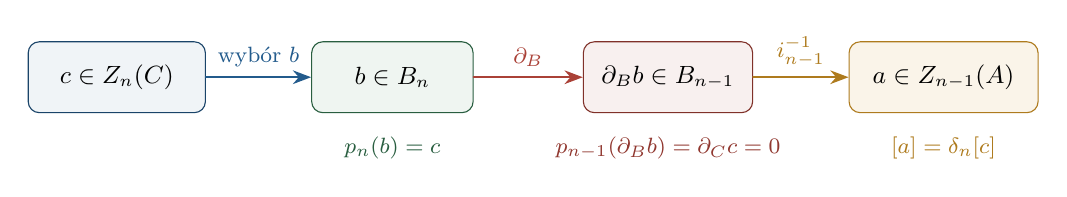
\begin{tikzpicture}[>=Stealth,line cap=round,
  every node/.style={font=\small}]
 \node[draw=manifoldblue!75!black,rounded corners,
  fill=manifoldblue!7,minimum width=2.25cm,
  minimum height=.9cm] (c) at (-5.25,0) {$c\in Z_n(C)$};
 \node[draw=manifoldgreen!75!black,rounded corners,
  fill=manifoldgreen!8,minimum width=2.05cm,
  minimum height=.9cm] (b) at (-1.75,0) {$b\in B_n$};
 \node[draw=manifoldred!75!black,rounded corners,
  fill=manifoldred!8,minimum width=2.15cm,
  minimum height=.9cm] (db) at (1.75,0) {$\partial_Bb\in B_{n-1}$};
 \node[draw=manifoldgold!85!black,rounded corners,
  fill=manifoldgold!10,minimum width=2.4cm,
  minimum height=.9cm] (a) at (5.25,0) {$a\in Z_{n-1}(A)$};
 \draw[->,thick,manifoldblue] (c) --
  node[midway,above,font=\footnotesize] {wybór $b$} (b);
 \draw[->,thick,manifoldred] (b) --
  node[midway,above,font=\footnotesize] {$\partial_B$} (db);
 \draw[->,thick,manifoldgold!85!black] (db) --
  node[midway,above,font=\footnotesize] {$i_{n-1}^{-1}$} (a);
 \node[font=\footnotesize,manifoldgreen!75!black]
  at (-1.75,-.9) {$p_n(b)=c$};
 \node[font=\footnotesize,manifoldred!85!black]
  at (1.75,-.9) {$p_{n-1}(\partial_Bb)=\partial_Cc=0$};
 \node[font=\footnotesize,manifoldgold!85!black]
  at (5.25,-.9) {$[a]=\delta_n[c]$};
\end{tikzpicture}
\caption{Odwzorowanie łączące: podnosimy cykl $c$, bierzemy brzeg
podniesienia $b$, po czym odczytujemy go w $A_{n-1}$.
Odwrócenie $i_{n-1}$ dotyczy tylko jego obrazu
$\ker p_{n-1}$; całego odwzorowania $i_{n-1}$ nie odwracamy.}
\label{fig:homologia-delta}
\end{figure}

\begin{twierdzenie}[Długi ciąg dokładny]
\label{thm:les-homologia}
Z krótkiego ciągu dokładnego kompleksów
otrzymujemy naturalny długi ciąg dokładny
\begin{equation}\label{eq:les-homologia}
 \cdots\longrightarrow H_n(A)
 \xrightarrow{i_*}H_n(B)
 \xrightarrow{p_*}H_n(C)
 \xrightarrow{\delta_n}H_{n-1}(A)
 \xrightarrow{i_*}H_{n-1}(B)
 \longrightarrow\cdots.
\end{equation}
Odwzorowanie \emph{łączące} $\delta_n$ ma następujący
konkretny wzór. Dla cyklu $c\in C_n$ wybieramy
podniesienie $b\in B_n$ z $p_n(b)=c$.
Wtedy $\partial_B b=i_{n-1}(a)$ dla dokładnie
jednego $a\in A_{n-1}$, a
\begin{equation}\label{eq:delta-wzor}
 \delta_n[c]=[a]\in H_{n-1}(A).
\end{equation}
Jeżeli kompleksy są zerowe w ujemnych stopniach,
końcowy fragment ma postać
$H_0(A)\to H_0(B)\to H_0(C)\to0$.
\end{twierdzenie}
\begin{proof}
\emph{Konstrukcja i cykl.} Surjektywność $p_n$
daje podniesienie $b$. Ponieważ $p$ jest odwzorowaniem łańcuchowym,
\[
 p_{n-1}(\partial_Bb)=\partial_C(p_nb)=\partial_Cc=0.
\]
Z dokładności~\eqref{eq:ses-kompleks} w
stopniu $n-1$ mamy
$\partial_Bb\in\ker p_{n-1}=\operatorname{im}i_{n-1}$,
więc istnieje $a$ z $i_{n-1}a=\partial_Bb$.
Iniektywność $i_{n-1}$ daje jego jednoznaczność.
Ponadto
\[
 i_{n-2}(\partial_Aa)
 =\partial_B(i_{n-1}a)=\partial_B^2b=0.
\]
Iniektywność $i_{n-2}$ wymusza $\partial_Aa=0$.
Możemy więc wziąć klasę $[a]$.

\emph{Niezależność od podniesienia.} Jeśli $b'$ też
podnosi $c$, to $b'-b=i_n(u)$ dla pewnego
$u\in A_n$. Wtedy
\[
 \partial_Bb'=\partial_Bb+\partial_Bi_nu
 =i_{n-1}(a+\partial_Au).
\]
Nowy cykl w $A$ różni się od $a$ o brzeg,
więc wyznacza tę samą klasę.

\emph{Niezależność od reprezentanta.}
Niech $c'=c+\partial_Cv$, $v\in C_{n+1}$.
Wybierzmy podniesienie $w\in B_{n+1}$ elementu $v$.
Wtedy $b+\partial_Bw$ podnosi $c'$ i ma ten sam
brzeg co $b$, bo $\partial_B^2w=0$.
Każde inne podniesienie $c'$ różni się od tego
o element $\operatorname{im}i_n$; właśnie
sprawdzona niezależność od podniesienia
kończy dowód niezależności od wyboru reprezentanta klasy $[c]$.
Suma podniesień podnosi sumę cykli, a
podniesienie $rb$ podnosi $rc$, więc $\delta_n$
jest homomorfizmem $R$-modułów.

\emph{Dokładność przy $H_n(B)$.}
Z $pi=0$ mamy $p_*i_*=0$.
Jeśli $[b]\in H_n(B)$ spełnia
$p_*[b]=0$, to dla cyklu $b$
istnieje $v\in C_{n+1}$ z
$p_nb=\partial_Cv$. Wybierzmy podniesienie
$w\in B_{n+1}$ elementu $v$.
Wtedy $b'=b-\partial_Bw$ nadal jest cyklem,
$[b']=[b]$ i
$p_nb'=p_nb-\partial_Cv=0$. Z dokładności
w stopniu $n$ mamy $b'=i_na$.
Ponieważ $\partial_Bb'=i_{n-1}\partial_Aa=0$
i $i_{n-1}$ jest iniektywna, $a$ jest
cyklem. Stąd $[b]=i_*[a]$.

\emph{Dokładność przy $H_n(C)$.}
Jeżeli $c=p_nb$ dla cyklu $b$, możemy
w definicji $\delta_n$ wybrać to właśnie
podniesienie: $\partial_Bb=0$, więc $\delta_n[c]=0$.
Odwrotnie, załóżmy $\delta_n[c]=0$
i podnieśmy cykl $c$ do $b$.
Jeśli $\partial_Bb=i_{n-1}a$, to $[a]=0$,
czyli $a=\partial_Au$ dla pewnego $u\in A_n$.
Element $b-i_nu$ jest cyklem, bo
$\partial_B(b-i_nu)=i_{n-1}(a-\partial_Au)=0$,
a $p_n(b-i_nu)=c$. Zatem
$[c]=p_*[b-i_nu]$.

\emph{Dokładność przy $H_{n-1}(A)$.}
Dla klasy $\delta_n[c]=[a]$ mamy
$i_{n-1}a=\partial_Bb$, czyli $i_*[a]=0$.
Odwrotnie, jeżeli $a\in Z_{n-1}(A)$
i $i_*[a]=0$, istnieje $b\in B_n$
takie, że $i_{n-1}a=\partial_Bb$.
Wówczas $c=p_nb$ jest cyklem, bo
$\partial_Cc=p_{n-1}\partial_Bb=p_{n-1}i_{n-1}a=0$,
a wzór~\eqref{eq:delta-wzor} daje
$\delta_n[c]=[a]$.
Przesuwając indeks $n$ o jeden,
obejmujemy tymi trzema sprawdzeniami
każde miejsce całego ciągu~\eqref{eq:les-homologia}.
W końcu, przy założonej zerowości kompleksów w ujemnych
stopniach mamy $A_{-1}=0$, a więc
$H_{-1}(A)=0$, więc $H_0(B)\to H_0(C)$
jest surjekcją na mocy właśnie wykazanej
dokładności.
\end{proof}

\begin{uwaga}[Naturalność odwzorowania łączącego]
\label{uwaga:les-naturalnosc}
Jeżeli mamy odwzorowanie między dwoma krótkimi
ciągami kompleksów, zgodne z $i,p$ i
różniczkami, to odwzorowania na homologiach
komutują także z $\delta$.
Dokładniej, są to odwzorowania łańcuchowe
$f_A:A\to A'$, $f_B:B\to B'$, $f_C:C\to C'$ spełniające
$f_Bi=i'f_A$ oraz $p'f_B=f_Cp$.
Istotnie, podniesienie $b$ cyklu $c$ przechodzi
w podniesienie obrazu $c$, jego brzeg przechodzi
w obraz $\partial_Bb$, a wstrzyknięcie $i$
pozwala odczytać obraz tego samego $a$.
Równość na reprezentantach ma postać
$\delta'_n(H_n(f_C)[c])
=H_{n-1}(f_A)(\delta_n[c])$.
\end{uwaga}

\begin{przyklad}[Niezerowe odwzorowanie łączące]
\label{prz:delta-izomorfizm}
Niech $A_\bullet$ ma jedyny niezerowy moduł
$A_0=R$, a $C_\bullet$ jedyny niezerowy
moduł $C_1=R$. Niech $B_\bullet$ ma
$B_1=B_0=R$ i różniczkę
$\partial_B=\id_R:B_1\to B_0$.
W stopniu $0$ odwzorowanie $i_0:A_0\to B_0$
jest identycznością, a w stopniu $1$
odwzorowanie $p_1:B_1\to C_1$ jest identycznością;
pozostałe odwzorowania to jedyne możliwe odwzorowania zerowe.
W każdym stopniu otrzymujemy rozszczepiony
krótki ciąg dokładny modułów, ale
$H_n(B)=0$ we wszystkich stopniach.
Cykl $c=1\in C_1$ podnosimy do $b=1\in B_1$.
Jego brzeg to $1=i_0(1)\in B_0$,
więc $\delta_1:R\to R$ jest identycznością.
Przykład pokazuje, że stopniowe rozszczepienie
nie oznacza zgodnego z różniczkami
rozszczepienia kompleksów.
\end{przyklad}
\section{Kohomologia algebraiczna i jej długi ciąg}
\label{sec:kohomologia-algebraiczna}

W homologii różniczka obniża stopień.
Kohomologia powstaje z równie prostej
konstrukcji, w której różniczka stopień
\emph{podwyższa}. Gdy elementy kompleksu
łańcuchowego są wektorami, elementy
kompleksu dualnego są funkcjonałami:
zamiast brać brzeg wektora, oceniamy
funkcjonał na brzegu.

\begin{definicja}[Kompleks kołańcuchowy i kohomologia]
\index{kompleks kolancuchowy i kohomologia@Kompleks kołańcuchowy i kohomologia}
\label{def:kohomologia-algebraiczna}
\emph{Kompleks kołańcuchowy} $K^\bullet$ to
moduły $K^n$ i homomorfizmy
$d^n:K^n\to K^{n+1}$ z
$d^{n+1}d^n=0$ dla $n\in\Z$. Jego \emph{kohomologią stopnia $n$}
jest
\begin{equation}\label{eq:kohomologia-def}
 H^n(K):=\frac{\ker(d^n:K^n\to K^{n+1})}
 {\operatorname{im}(d^{n-1}:K^{n-1}\to K^n)}.
\end{equation}
Elementy jądra nazywamy \emph{kocyklami},
a elementy obrazu \emph{kobrzegami}.
Odwzorowanie kołańcuchowe $F:K^\bullet\to L^\bullet$
składa się z $F^n:K^n\to L^n$ spełniających
$d_L^nF^n=F^{n+1}d_K^n$.
\end{definicja}

Tak jak w dowodzie
Stwierdzenia~\ref{prop:homologia-funktor},
odwzorowanie kołańcuchowe przenosi kocykle w
kocykle i kobrzegi w kobrzegi:
$d_LFz=Fdz=0$ oraz
$F(d_Ku)=d_L(Fu)$. Wobec tego definiuje
$H^n(F)[z]=[F^nz]$. Równość
$H^n(K)=0$ mówi dokładnie, że
$K^{n-1}\to K^n\to K^{n+1}$
jest dokładny w $K^n$.

\begin{przyklad}[Kohomologia dwuwyrazowego kompleksu]
Dla $K^0=K^1=\Z$, $d^0=\times2$
i wszystkich innych modułów równych $0$
otrzymujemy $H^0(K)=0$ oraz
$H^1(K)=\Z/2\Z$. W stopniu $1$ nie ma
już różniczki wychodzącej, więc
wszystkie elementy $\Z$ są kocyklami;
kobrzegami są liczby parzyste.
\end{przyklad}

\begin{stwierdzenie}[Kompleks dualny]
\label{prop:kompleks-dualny}
Dla kompleksu łańcuchowego $C_\bullet$
i $R$-modułu $G$ połóżmy
\[
 C^n(C;G):=\operatorname{Hom}_R(C_n,G),
 \qquad d^n\varphi:=\varphi\circ \partial_{n+1}.
\]
Wtedy $C^\bullet(C;G)$ jest kompleksem
kołańcuchowym. Odwzorowanie łańcuchowe
$f:C_\bullet\to D_\bullet$ daje odwzorowanie
kołańcuchowe w odwrotną stronę,
$f^*:C^\bullet(D;G)\to C^\bullet(C;G)$,
$f^*(\varphi)=\varphi\circ f_n$.
\end{stwierdzenie}
\begin{proof}
Dla $\varphi:C_n\to G$ mamy
\[
 d^{n+1}(d^n\varphi)
 =(\varphi\circ \partial_{n+1})\circ \partial_{n+2}
 =\varphi\circ(\partial_{n+1}\partial_{n+2})=0.
\]
Z kolei dla $\varphi:D_n\to G$
oraz $x\in C_{n+1}$ równość odwzorowań łańcuchowych
z~\eqref{eq:mapa-lancuchowa} daje
\[
 (d f^*\varphi)(x)
 =\varphi(f_n(\partial_C x))
 =\varphi(\partial_D(f_{n+1}x))
 =(f^*d\varphi)(x).
\]
To dowodzi zgodności z różniczką.
\end{proof}

Słowo \emph{dualny} wymaga tu ostrożności:
zastosowanie $\operatorname{Hom}_R(-,G)$
do krótkiego ciągu dokładnego modułów
nie musi dać krótkiego ciągu dokładnego.
Na przykład przy $G=\Z$ w ciągu
$0\to2\Z\hookrightarrow\Z\to\Z/2\Z\to0$
funkcjonał $2\Z\to\Z$, $2k\mapsto k$,
nie przedłuża się do homomorfizmu
$\Z\to\Z$: musiałby wysłać $1$
na liczbę $t$ z $2t=1$.
Z tego powodu nie będziemy budować
długiego ciągu kohomologii przez
bezrefleksyjne dualizowanie
Twierdzenia~\ref{thm:les-homologia}.

\begin{twierdzenie}[Długi ciąg kohomologii]
\label{thm:les-kohomologia}
Jeżeli w każdym stopniu dokładny jest
krótki ciąg \emph{kompleksów kołańcuchowych}
\[
 0\longrightarrow A^\bullet\xrightarrow{i}B^\bullet
 \xrightarrow{p}C^\bullet\longrightarrow0,
\]
to istnieje długi ciąg dokładny
\begin{equation}\label{eq:les-kohomologia}
 \cdots\longrightarrow H^n(A)
 \xrightarrow{i_*}H^n(B)
 \xrightarrow{p_*}H^n(C)
 \xrightarrow{\delta^n}H^{n+1}(A)
 \xrightarrow{i_*}H^{n+1}(B)\longrightarrow\cdots.
\end{equation}
\end{twierdzenie}
\begin{proof}
Dla kocyklu $c\in C^n$ wybierzmy podniesienie
$b\in B^n$ z $p(b)=c$.
Wtedy $p(d_Bb)=d_Cc=0$, więc dokładność
w stopniu $n+1$ i iniektywność $i$
dają dokładnie jedno $a\in A^{n+1}$
z $i(a)=d_Bb$.
Ponieważ $i(d_Aa)=d_B^2b=0$,
otrzymujemy kocykl $a$.
Definiujemy $\delta^n[c]=[a]$.
Jeśli podniesienie $b$ zastąpimy $b+i(u)$,
to $a$ zmienia się na $a+d_Au$.
Jeśli $c$ zastąpimy $c+d_Cv$, to po
wyborze podniesienia $w$ dla $v$ możemy
zastąpić $b$ przez $b+d_Bw$,
co w ogóle nie zmienia $d_Bb$.
Oba wybory prowadzą zatem do tej
samej klasy. Podniesienie sumy można wziąć
jako sumę podniesień, a $rb$ podnosi $rc$ dla $r\in R$.
Zatem $\delta^n$ jest $R$-liniowa.

Sprawdźmy każde z trzech rodzajów miejsc
w~\eqref{eq:les-kohomologia}.
Przy $H^n(B)$ mamy $p_*i_*=0$.
Jeśli $b\in B^n$ jest kocyklem
i $p_*[b]=0$, to $p(b)=d_Cv$
dla pewnego $v\in C^{n-1}$.
Podnieśmy $v$ do $w\in B^{n-1}$.
Wówczas $b-d_Bw$ jest kocyklem
z tą samą klasą co $b$, a jego
obraz przez $p$ wynosi $0$.
Równa się więc $i(a)$ dla pewnego
$a\in A^n$. Z $0=d_Bi(a)=i(d_Aa)$
i iniektywności $i$ dostajemy
$d_Aa=0$, a zatem $[b]=i_*[a]$.

Przy $H^n(C)$ inkluzja
$\operatorname{im}p_*\subseteq\ker\delta^n$
wynika z wybrania jako podniesienia $c=p(b)$
samego kocyklu $b$: jego różniczka jest $0$.
Jeśli odwrotnie $\delta^n[c]=0$,
to dla podniesienia $b$ mamy $d_Bb=i(a)$,
gdzie $a=d_Au$ dla pewnego $u\in A^n$.
Element $b-i(u)$ jest kocyklem,
którego obraz to $c$, więc
$[c]\in\operatorname{im}p_*$.

Przy $H^{n+1}(A)$ element
$i_*\delta^n[c]$ reprezentuje
$i(a)=d_Bb$ i dlatego jest zerowy.
Jeśli z drugiej strony $a\in A^{n+1}$
jest kocyklem i $i_*[a]=0$,
to $i(a)=d_Bb$ dla pewnego
$b\in B^n$. Obraz $c=p(b)$ jest
kocyklem, gdyż $d_Cc=p(d_Bb)=p(i(a))=0$,
a jego odwzorowanie łączące wynosi $[a]$.
Zmiana $n$ daje dokładność także
w pozostałych stopniach. Konstrukcja jest naturalna:
dla zgodnych odwzorowań $f_A,f_B,f_C$ między krótkimi ciągami
podniesieniem $f_C(c)$ jest $f_B(b)$, a jego różniczka to
$f_B(d_Bb)=f_B(i(a))=i'(f_A(a))$.
Stąd $\delta'^n H^n(f_C)=H^{n+1}(f_A)\delta^n$.
\end{proof}

\begin{twierdzenie}[Nad ciałem kohomologia jest dualna do homologii]
\label{thm:field-hom-dual}
Niech $C_\bullet$ będzie kompleksem
przestrzeni liniowych nad ciałem
$\mathbb K$, a
$C^n=\operatorname{Hom}_{\mathbb K}(C_n,\mathbb K)$.
Wtedy naturalne przypisanie
\begin{equation}\label{eq:field-duality}
 H^n(C^\bullet)
 \longrightarrow\operatorname{Hom}_{\mathbb K}
  (H_n(C_\bullet),\mathbb K),
 \qquad [\varphi]\longmapsto
     ([z]\longmapsto\varphi(z))
\end{equation}
jest izomorfizmem. Zakładamy, że
przestrzenie pozwalają na wybór
dopełnień podprzestrzeni
(w szczególności wystarcza skończony wymiar).
\end{twierdzenie}
\begin{proof}
Jeżeli $\varphi\in C^n$ jest kocyklem,
to $d^n\varphi=\varphi \partial_{n+1}=0$.
Zatem $\varphi$ znika na $B_n$,
więc jej wartość na $z\in Z_n$
zależy tylko od klasy $[z]\in H_n$.
Jeżeli zmienimy $\varphi$ na
$\varphi+d^{n-1}\psi
=\varphi+\psi \partial_n$, to dla cyklu $z$
mamy $\partial_nz=0$, więc otrzymujemy
ten sam funkcjonał na $H_n$.
Odwzorowanie~\eqref{eq:field-duality} jest
dobrze określone i liniowe. Jest też naturalne: dla odwzorowania
łańcuchowego $f:C\to D$, kocyklu $\varphi$ na $D$ i cyklu $z$ na $C$
mamy $(f^*\varphi)(z)=\varphi(fz)$. Zatem obie drogi, przez
$H^n(f^*)$ lub przez prekompozycję z $H_n(f)$, dają ten sam funkcjonał.

Aby pokazać surjektywność, weźmy
$\ell:H_n=Z_n/B_n\to\mathbb K$.
Złożenie $Z_n\to H_n\xrightarrow{\ell}\mathbb K$
jest liniowe i znika na $B_n$.
Wybieramy dopełnienie $Z_n$ w $C_n$
i przedłużamy funkcjonał liniowo
na $C_n$, na przykład jako zero
na tym dopełnieniu. Otrzymany
$\varphi$ spełnia
$\varphi \partial_{n+1}=0$, bo
$\operatorname{im}\partial_{n+1}=B_n$;
jest kocyklem wysyłanym na $\ell$.

Jeżeli klasa $[\varphi]$ trafia na zero,
to $\varphi$ znika na całym $Z_n$.
Możemy więc zdefiniować funkcjonał
$\eta$ na $B_{n-1}=\operatorname{im}\partial_n$
przez $\eta(\partial_nx)=\varphi(x)$.
Jest dobrze określony: z
$\partial_nx=\partial_nx'$ wynika $x-x'\in Z_n$,
a tam $\varphi$ znika.
Wybieramy dopełnienie $B_{n-1}$
w $C_{n-1}$ i przedłużamy $\eta$
do $\psi:C_{n-1}\to\mathbb K$.
Wtedy $\varphi=\psi \partial_n=d^{n-1}\psi$
jest kobrzegiem. Jądro odwzorowania
w~\eqref{eq:field-duality} jest więc zerowe.
\end{proof}

\begin{uwaga}[Dlaczego ważne są współczynniki?]
Nad $\Z$ odpowiednik~\eqref{eq:field-duality}
może być fałszywy. Dla kompleksu
$C_1=C_0=\Z$ z $\partial_1=\times2$ mamy
$H_0(C)=\Z/2$ i $H_1(C)=0$,
podczas gdy dla dualnego kompleksu
$H^1(C^\bullet)=\Z/2$.
Grupa $\operatorname{Hom}_{\Z}
(H_1(C),\Z)$ jest zerowa.
Ta dodatkowa klasa kohomologii
wykrywa informację torsyjną z
poprzedniego stopnia. Nie utożsamiamy
więc homologii z kohomologią bez
sprawdzenia założeń o współczynnikach.
\end{uwaga}
\section{Homotopia łańcuchowa i uproszczenia kompleksów}
\label{sec:homotopia-lancuchowa}

Jedna homologia może mieć bardzo różne opisy
przez generatory i różniczki. Poniższe kryterium
mówi, kiedy dwa odwzorowania kompleksów dają
\emph{dokładnie to samo} odwzorowanie na
homologiach. Jest to algebraiczny mechanizm
usuwania par generatorów, które wzajemnie
się kasują.

\begin{definicja}[Homotopia łańcuchowa]
\index{homotopia lancuchowa@Homotopia łańcuchowa}
\label{def:homotopia-lancuchowa}
Dwa odwzorowania łańcuchowe $f,g:C_\bullet\to D_\bullet$
są \emph{łańcuchowo homotopijne}, jeśli istnieją
homomorfizmy $R$-modułów $h_n:C_n\to D_{n+1}$ takie, że
\begin{equation}\label{eq:chain-homotopy}
 f_n-g_n=\partial^D_{n+1}h_n+h_{n-1}\partial^C_n
 \qquad\text{dla każdego }n.
\end{equation}
Kompleks $C_\bullet$ jest \emph{ściągalny},
jeśli $\id_C$ jest łańcuchowo homotopijna
z odwzorowaniem zerowym.
\end{definicja}

Wzór~\eqref{eq:chain-homotopy} przypomina
zasadę całkowania przez części: różnica
odwzorowań składa się z dwóch operacji, w których
$h$ i $\partial$ występują w przeciwnych
kolejnościach. Na cyklach drugi składnik
znika, a pierwszy jest brzegiem.

\begin{twierdzenie}[Homotopia nie zmienia homologii]
\label{thm:homotopia-homologia}
Jeśli $f$ i $g$ są łańcuchowo homotopijne,
to $H_n(f)=H_n(g)$ dla każdego $n$.
W szczególności kompleks ściągalny jest
acykliczny. Jeśli istnieją odwzorowania łańcuchowe
$f:C_\bullet\to D_\bullet$ i
$g:D_\bullet\to C_\bullet$ z
$gf\simeq\id_C$ i $fg\simeq\id_D$,
to $H_n(f)$ i $H_n(g)$ są wzajemnymi
izomorfizmami.
\end{twierdzenie}
\begin{proof}
Dla $z\in Z_n(C)$ równanie~\eqref{eq:chain-homotopy}
redukuje się do
\[
 f_n(z)-g_n(z)=\partial^D_{n+1}h_n(z),
\]
bo $\partial^C_nz=0$. Różnica obrazów jest
brzegiem, więc $[f_n(z)]=[g_n(z)]$.
Gdy $f=\id_C$, $g=0$, otrzymujemy
$[z]=[0]$ dla każdej klasy, czyli
$H_n(C)=0$.
Na koniec, dzięki
Stwierdzeniu~\ref{prop:homologia-funktor},
\[
 H_n(g)H_n(f)=H_n(gf)
 =H_n(\id_C)=\id,\qquad
 H_n(f)H_n(g)=\id.
\]
Stąd oba odwzorowania na homologiach są
odwrotne do siebie.
\end{proof}

\begin{przyklad}[Najprostsze ściągnięcie]
Dla kompleksu
$0\to R\xrightarrow{\id}R\to0$
z modułami w stopniach $1$ i $0$
połóżmy $h_0:R=C_0\to C_1=R$
równe identyczności, a pozostałe
$h_n=0$. W stopniu $0$ mamy
$\partial_1h_0=\id_{C_0}$, a w stopniu
$1$ mamy $h_0\partial_1=\id_{C_1}$.
Wzór~\eqref{eq:chain-homotopy}
daje $\id_C=\partial h+h\partial$.
\end{przyklad}

\begin{twierdzenie}[Algebraiczne skasowanie pary generatorów]
\label{thm:kasowanie-pary}
Niech $C_\bullet$ będzie kompleksem
wolnych $R$-modułów z ustalonymi
bazami, a $n\geq1$. Załóżmy, że
przy generatorze $f\in C_{n-1}$
we współrzędnych $\partial_n(e)$ dla pewnego
generatora $e\in C_n$ stoi skalar
odwracalny $u\in R$.
Wtedy przez zmiany baz można rozłożyć
$C_\bullet$ na sumę prostą
podkompleksu i dwuwyrazowego kompleksu
\[
 0\longrightarrow R e
 \xrightarrow{\ \partial_n\ }R\,\partial_n(e)
 \longrightarrow0,
\]
w którym $\partial_n$ jest izomorfizmem.
Usunięcie tej pary nie zmienia homologii.
\end{twierdzenie}
\begin{proof}
Zapiszmy
$C_n=R e\oplus M$ oraz
$C_{n-1}=R f\oplus N$, gdzie
$M,N$ są rozpięte przez pozostałe
wybrane wektory bazowe.
Z założenia
$\partial_n(e)=u f+v$ z $v\in N$.
Ponieważ $u$ jest odwracalny,
$f':=\partial_n(e)$ może zastąpić $f$
w bazie $C_{n-1}$:
$C_{n-1}=R f'\oplus N$.
Rzeczywiście, $f=u^{-1}(f'-v)$
pozwala przejść w obie strony
między rozkładami.

Dla $x\in M$ zapiszmy
$\partial_n(x)=a(x)f+w(x)$,
gdzie $a(x)\in R$ i $w(x)\in N$.
Zmieńmy też bazę w stopniu $n$,
zastępując każdy bazowy $x\in M$
wektorem $x':=x-u^{-1}a(x)e$.
Wtedy
\[
 \partial_n(x')
 =a(x)f+w(x)-u^{-1}a(x)(uf+v)
 =w(x)-u^{-1}a(x)v\in N.
\]
Nowe wektory $x'$ razem z $e$
tworzą bazę $C_n$: możemy odzyskać
$x=x'+u^{-1}a(x)e$.
Oznaczmy ich rozpiętość przez $M'$.
Mamy zatem $\partial_n(Re)=Rf'$
i $\partial_n(M')\subseteq N$.

Równość $\partial_{n-1}(f')=\partial_{n-1}\partial_n(e)=0$
mówi, że z $Rf'$ nie wychodzi
różniczka. Z kolei dla $y\in C_{n+1}$
zapiszmy $\partial_{n+1}(y)=t e+x'$,
$x'\in M'$. Po zastosowaniu $\partial_n$
dostajemy
$0=\partial_n\partial_{n+1}(y)=t f'+\partial_n(x')$.
Pierwszy składnik należy do $Rf'$,
drugi do $N$; rozkład jest prosty,
więc $t=0$. Żadna różniczka
z wyższego stopnia nie trafia do $Re$.
Pozostałe moduły wraz z $M'$ i $N$
tworzą więc podkompleks, a
$Re\xrightarrow{\cong}Rf'$
jest jego prostym składnikiem
w całym kompleksie.

Na tym dwuwyrazowym składniku
homotopia $h_{n-1}(f')=e$,
zerowa w innych stopniach,
spełnia $\id=\partial h+h\partial$.
Jest on ściągalny. Przedłużmy tę homotopię przez zero na
pozostałym podkompleksie $D$. Dla rzutu $p:C\to D$ i włączenia
$j:D\to C$ otrzymujemy $pj=\id_D$ oraz
$\id_C-jp=\partial h+h\partial$. Rzut i włączenie
wyznaczają odwrotne izomorfizmy
na homologiach na mocy
Twierdzenia~\ref{thm:homotopia-homologia}.
\end{proof}

Nad $\Z$ jednostkami są tylko $1$ i $-1$.
Współczynnik $2$ w różniczce
$\Z\xrightarrow{\times2}\Z$ nie pozwala
wykonać takiego skasowania: pozostała
klasa $\Z/2$ z
Przykładu~\ref{prz:homologia-rachunki}
jest rzeczywistą przeszkodą.

\begin{stwierdzenie}[Acykliczny kompleks przestrzeni liniowych]
\label{prop:acykliczny-sciagalny}
Jeżeli $C_\bullet$ jest kompleksem
przestrzeni liniowych nad ciałem
$\mathbb K$ i $H_n(C)=0$ dla wszystkich
$n$, to $C_\bullet$ jest ściągalny.
Wystarczy, aby każda podprzestrzeń
$Z_n(C)\subseteq C_n$ miała dopełnienie;
warunek ten zachodzi zawsze przy
skończonych wymiarach.
\end{stwierdzenie}
\begin{proof}
Acykliczność daje $Z_n=B_n$.
Wybierzmy dopełnienie $S_n$ tak, aby
$C_n=Z_n\oplus S_n$. Ograniczenie
\[
 \partial_n|_{S_n}:S_n\longrightarrow Z_{n-1}
\]
jest iniektywne: element jego jądra
należy do $S_n\cap Z_n=\{0\}$.
Jest też surjektywne, bo
$\partial_n(C_n)=B_{n-1}=Z_{n-1}$
i $\partial_n$ znika na $Z_n$.
Ma więc odwrotność.
Każde $x\in C_n$ zapiszmy
jednoznacznie jako $x=z+s$
z $z\in Z_n$, $s\in S_n$, i połóżmy
\[
 h_n(z+s)
 :=(\partial_{n+1}|_{S_{n+1}})^{-1}(z)
 \in S_{n+1}.
\]
Wówczas $\partial_{n+1}h_n(z+s)=z$.
Z drugiej strony $\partial_n(z+s)=\partial_n(s)$,
więc
$h_{n-1}\partial_n(z+s)
=(\partial_n|_{S_n})^{-1}(\partial_ns)=s$.
Zatem $(\partial h+h\partial)(x)=z+s=x$
w każdym stopniu.
\end{proof}

\begin{przyklad}[Acykliczny, lecz nieściągalny nad $\Z$]
\label{prz:acykliczny-niesciagalny}
Potraktujmy dokładny ciąg z
Przykładu~\ref{prz:ses-mod-m} dla $m=2$
jako kompleks w stopniach $2,1,0$:
\[
 0\longrightarrow\Z\xrightarrow{\ \times2\ }\Z
 \xrightarrow{\ \pi\ }\Z/2\Z\longrightarrow0.
\]
Jego wszystkie homologie są zerowe,
bo $\times2$ jest iniekcją,
$\ker\pi=2\Z$, a $\pi$ jest
surjekcją. Gdyby kompleks był
ściągalny, to w stopniu $0$
wzór $\id=\partial h+h\partial$ dałby
$\id_{\Z/2}=\pi h_0$.
Odwzorowanie $h_0:\Z/2\to\Z$ byłoby
przekrojem $\pi$, którego
nie ma według uwagi po
Twierdzeniu~\ref{thm:ses-rozszczepienie}.
Zatem implikacja \emph{acykliczny
$\Rightarrow$ ściągalny} wymaga
dodatkowych założeń. Implikacja
odwrotna z
Twierdzenia~\ref{thm:homotopia-homologia}
działa nad każdym pierścieniem.
\end{przyklad}

\section{Ilorazy, ciągi względne i filtracje}
\label{sec:iloraz-filtracja}

Podkompleks $A_\bullet\subseteq C_\bullet$
oznacza podmoduły $A_n\subseteq C_n$
we wszystkich stopniach, takie że
$\partial_C(A_n)\subseteq A_{n-1}$.
Definiujemy \emph{kompleks ilorazowy}
$(C/A)_n=C_n/A_n$ i
$\partial_{C/A}[c]=[\partial_Cc]$.
Jeśli $[c]=[c+a]$ dla $a\in A_n$,
to $[\partial_Cc]=[\partial_Cc+\partial_Ca]$;
różniczka ilorazowa jest dobrze
określona i jej kwadrat wynosi zero.

\begin{stwierdzenie}[Długi ciąg ilorazu]
\label{prop:ses-iloraz}
Dla podkompleksu $A_\bullet\subseteq C_\bullet$
ciąg
\[
 0\longrightarrow A_\bullet
 \longrightarrow C_\bullet
 \longrightarrow C_\bullet/A_\bullet
 \longrightarrow0
\]
jest stopniowo dokładny. Dlatego istnieje
długi ciąg
\begin{equation}\label{eq:les-iloraz}
 \cdots\to H_n(A)\to H_n(C)\to H_n(C/A)
 \xrightarrow{\delta_n}H_{n-1}(A)\to\cdots.
\end{equation}
Jeśli $\xi\in H_n(C/A)$, to możemy
reprezentować ją elementem $c\in C_n$
z $\partial_Cc\in A_{n-1}$, a wtedy
$\delta_n\xi=[\partial_Cc]$. Tutaj $c$ najpierw wyznacza cykl
$c+A_n$ w kompleksie ilorazowym, a dopiero jego klasa modulo
brzegi jest elementem $\xi$; są to dwa różne przejścia do ilorazu.
\end{stwierdzenie}
\begin{proof}
W każdym stopniu włączenie $A_n\to C_n$
jest iniekcją, projekcja $C_n\to C_n/A_n$
jest surjekcją, a jej jądrem jest $A_n$.
Oba odwzorowania komutują z różniczkami
z definicji podkompleksu i ilorazu.
Twierdzenie~\ref{thm:les-homologia}
stosuje się więc bez dodatkowych
założeń. Warunek
$\partial_{C/A}[c]=[0]$ jest równoważny
$\partial_Cc\in A_{n-1}$; w tej sytuacji
konstrukcja~\eqref{eq:delta-wzor}
przy podniesieniu $c$ daje dokładnie
klasę $[\partial_Cc]$.
\end{proof}

Symbol $H_n(C,A):=H_n(C/A)$ będziemy
nazywać \emph{względną homologią
algebraiczną} kompleksu $C$ względem
podkompleksu $A$. Jest to definicja
czysto algebraiczna. W przyszłych
konstrukcjach topologicznych trzeba
osobno sprawdzić, że odpowiednie
łańcuchy tworzą podkompleks.

\begin{stwierdzenie}[Względna kohomologia nad ciałem]
\label{prop:wzgledna-kohomologia}
Jeśli $A_\bullet\subseteq C_\bullet$
jest podkompleksem przestrzeni liniowych
nad ciałem $\mathbb K$, to wzięcie
funkcjonałów daje krótki ciąg dokładny
kompleksów kołańcuchowych
\[
 0\to\operatorname{Hom}_{\mathbb K}
      (C/A,\mathbb K)
 \to\operatorname{Hom}_{\mathbb K}(C,\mathbb K)
 \to\operatorname{Hom}_{\mathbb K}(A,\mathbb K)
 \to0.
\]
Jeśli $H^n(C,A;\mathbb K)$ oznacza
kohomologię pierwszego z nich, to mamy
długi ciąg
\[
 \cdots\to H^n(C,A;\mathbb K)\to H^n(C;\mathbb K)
 \to H^n(A;\mathbb K)\to H^{n+1}(C,A;\mathbb K)
 \to\cdots .
\]
W tym zapisie $H^n(C;\mathbb K)$
oznacza kohomologię kompleksu
$\operatorname{Hom}_{\mathbb K}(C,\mathbb K)$,
a analogicznie dla $A$.
\end{stwierdzenie}
\begin{proof}
W stopniu $n$ pierwsze odwzorowanie składa
funkcjonał $C_n/A_n\to\mathbb K$
z projekcją $C_n\to C_n/A_n$,
więc jest iniektywne.
Drugie ogranicza funkcjonał na $C_n$
do podprzestrzeni $A_n$.
Jego jądrem są dokładnie funkcjonały
znikające na $A_n$, czyli faktoryzujące
się przez $C_n/A_n$; to obraz
pierwszego odwzorowania. Każdy funkcjonał
na $A_n$ przedłuża się do $C_n$:
wybieramy dopełnienie $A_n$
i stawiamy na nim wartość $0$.
Drugie odwzorowanie jest zatem surjektywne.
Odwzorowania komutują z różniczkami
kołańcuchowymi, bo są zdefiniowane
przez składanie z odwzorowaniami łańcuchowymi.
Stosujemy
Twierdzenie~\ref{thm:les-kohomologia}.
\end{proof}

\begin{stwierdzenie}[Trzy zagnieżdżone kompleksy]
\label{prop:les-potrojny}
Jeśli $A_\bullet\subseteq B_\bullet
\subseteq C_\bullet$, to istnieje
krótki ciąg dokładny kompleksów
\[
 0\longrightarrow B_\bullet/A_\bullet
 \longrightarrow C_\bullet/A_\bullet
 \longrightarrow C_\bullet/B_\bullet
 \longrightarrow0
\]
i wynikający z niego długi ciąg
\[
 \cdots\to H_n(B,A)\to H_n(C,A)\to H_n(C,B)
 \to H_{n-1}(B,A)\to\cdots.
\]
\end{stwierdzenie}
\begin{proof}
W stopniu $n$ pierwsze odwzorowanie
$[b]_A\mapsto[b]_A$ jest iniektywne:
jeśli $[b]_A=0$ w $C_n/A_n$, to
$b\in A_n$, więc była już zerowa w
$B_n/A_n$. Ostatnie odwzorowanie
$[c]_A\mapsto[c]_B$ jest dobrze
określone, bo $A_n\subseteq B_n$,
i surjektywne, bo każda klasa modulo
$B_n$ ma reprezentanta $c\in C_n$.
Jej jądro składa się z klas
$[c]_A$ z $c\in B_n$, czyli jest
obrazem pierwszego odwzorowania.
Różniczki zachowują wszystkie trzy
podkompleksy, więc są to odwzorowania
kompleksów. Stosujemy
Twierdzenie~\ref{thm:les-homologia}.
\end{proof}

\begin{definicja}[Filtracja kompleksu]
\index{filtracja kompleksu@Filtracja kompleksu}
\label{def:filtracja-kompleksu}
Przez \emph{skończoną filtrację rosnącą} rozumiemy tutaj ciąg
podkompleksów
\[
 0=F_{-1}C_\bullet\subseteq
 F_0C_\bullet\subseteq\cdots\subseteq
 F_NC_\bullet=C_\bullet.
\]
Iloraz $F_pC/F_{p-1}C$ opisuje
algebraicznie \emph{nową warstwę}
w kroku $p$. W każdym kroku mamy
krótki ciąg dokładny
$0\to F_{p-1}C\to F_pC\to
F_pC/F_{p-1}C\to0$
i odpowiadający mu długi ciąg homologii.
\end{definicja}

\begin{wniosek}[Zmiana skoncentrowana w jednym stopniu]
\label{wn:filtracja-jeden-stopien}
Niech $A\subseteq B$ będzie podkompleksem
w nieujemnych stopniach i niech
$H_j(B/A)=0$ dla $j\ne q$, $q\geq1$.
Wówczas $H_j(A)\to H_j(B)$ jest
izomorfizmem dla $j\notin\{q,q-1\}$,
a pozostałe zmiany opisuje ciąg
\begin{equation}\label{eq:jedna-warstwa}
 0\to H_q(A)\to H_q(B)\to H_q(B/A)
 \xrightarrow{\delta_q}H_{q-1}(A)
 \to H_{q-1}(B)\to0.
\end{equation}
\end{wniosek}
\begin{proof}
Dla dowolnego $j$ wytnijmy z~\eqref{eq:les-iloraz}
fragment
\[
 H_{j+1}(B/A)\to H_j(A)\to H_j(B)\to H_j(B/A).
\]
Jeśli oba zewnętrzne moduły są zerowe,
środkowe odwzorowanie jest jednocześnie
iniektywne i surjektywne.
Tak jest, gdy $j\ne q,q-1$.
Dla $j=q$ i $j=q-1$ zachowujemy
pełen fragment długiego ciągu.
Jego lewa skrajna strzałka wychodzi
z $H_{q+1}(B/A)=0$, a prawa
wchodzi do $H_{q-1}(B/A)=0$,
co daje dokładnie~\eqref{eq:jedna-warstwa}.
\end{proof}

\begin{uwaga}[Co mówi odwzorowanie łączące?]
W~\eqref{eq:jedna-warstwa} element
nowej warstwy może zwiększyć
$H_q(B)$, jeśli ma zerowy obraz
przez $\delta_q$. Może też sprawić,
że wcześniejsza klasa w
$H_{q-1}(A)$ stanie się brzegiem:
tak dzieje się, jeśli leży w
$\operatorname{im}\delta_q$.
Ten jeden fragment ciągu odróżnia
\emph{powstanie klasy} od
\emph{zabicia klasy}, bez odwoływania
się do szczególnej realizacji
geometrycznej kompleksu.
\end{uwaga}
\section{Suma podkompleksów i ciąg Mayera--Vietorisa}
\label{sec:mv-algebraiczny}

Przy rozbiciu obiektu na dwie części trzeba
uwzględnić elementy wspólne: bez tego
zliczylibyśmy je dwa razy. Poniższy wynik
jest czysto algebraicznym źródłem
późniejszych ciągów Mayera--Vietorisa.
Nie wymaga jeszcze żadnej konstrukcji
łańcuchów z przestrzeni topologicznej.

\begin{twierdzenie}[Algebraiczny Mayer--Vietoris]
\label{thm:mv-algebraiczny}
Niech $A_\bullet$ i $B_\bullet$ będą
podkompleksami $C_\bullet$. Wtedy
$A\cap B$ i $A+B$ też są podkompleksami,
a ciąg
\begin{equation}\label{eq:mv-ses}
 0\longrightarrow A\cap B
 \xrightarrow{\ j\ }A\oplus B
 \xrightarrow{\ q\ }A+B
 \longrightarrow0,
 \quad j(x)=(x,-x),\quad q(a,b)=a+b
\end{equation}
jest krótkim ciągiem dokładnym kompleksów.
W szczególności mamy długi ciąg dokładny
\begin{equation}\label{eq:mv-les}
 \cdots\to H_n(A\cap B)\to H_n(A)\oplus H_n(B)
 \to H_n(A+B)\xrightarrow{\delta}
 H_{n-1}(A\cap B)\to\cdots.
\end{equation}
Jeśli cykl $c\in(A+B)_n$ zapiszemy
$c=a+b$ z $a\in A_n$, $b\in B_n$,
to $\delta[c]=[\partial a]=[-\partial b]$.
\end{twierdzenie}
\begin{proof}
Jeśli $x\in A_n\cap B_n$, to
$\partial x\in A_{n-1}$ i $\partial x\in B_{n-1}$,
więc $\partial$ zachowuje przecięcie.
Podobnie $\partial(a+b)=\partial a+\partial b$ należy do
$A_{n-1}+B_{n-1}$, zatem suma
też jest podkompleksem.
Różniczka w $A\oplus B$ działa
składowo, dlatego
$\partial\,j(x)=(\partial x,-\partial x)=j(\partial x)$ i
$\partial\,q(a,b)=\partial(a+b)=q(\partial a,\partial b)$.
Są to odwzorowania łańcuchowe.

W każdym stopniu odwzorowanie $j$ jest
iniektywne, bo $j(x)=(0,0)$
implikuje $x=0$. Odwzorowanie $q$ jest
surjektywne na $A_n+B_n$ z samej
definicji sumy. Jeśli $q(a,b)=0$,
to $a=-b$ należy jednocześnie do
$A_n$ i do $B_n$, a para ma postać
$(a,-a)=j(a)$. Stąd
$\ker q=\operatorname{im}j$.
Twierdzenie~\ref{thm:les-homologia}
daje~\eqref{eq:mv-les}. Używamy przy tym kanonicznego izomorfizmu
$H_n(A\oplus B)\cong H_n(A)\oplus H_n(B)$:
różniczka działa składowo, więc cykle i brzegi są odpowiednio
$Z_n(A)\oplus Z_n(B)$ i $B_n(A)\oplus B_n(B)$,
a $[(a,b)]\mapsto([a],[b])$ jest izomorfizmem ich ilorazów.

Na koniec, jeśli $\partial(a+b)=0$, to
$\partial a=-\partial b$. Lewa strona należy do
$A_{n-1}$, prawa do $B_{n-1}$,
więc obie są elementem $A\cap B$.
W konstrukcji odwzorowania łączącego
podniesienie cyklu $c$ jest parą $(a,b)$,
a jej brzeg $(\partial a,\partial b)=(\partial a,-\partial a)$
jest obrazem $j(\partial a)$. To daje
podany wzór i objaśnia znak.
\end{proof}

\begin{przyklad}[Niezerowy brzeg z przecięcia]
\label{prz:mv-niezerowa-delta}
Nad ciałem $\mathbb K$ weźmy kompleks
z $C_1=\mathbb K u\oplus\mathbb K v$,
$C_0=\mathbb K x\oplus\mathbb K y$,
$\partial(u)=x-y$ i $\partial(v)=y-x$,
zerowy w pozostałych stopniach.
Niech $A_1=\mathbb K u$, $B_1=\mathbb K v$,
ale $A_0=B_0=C_0$. Są to podkompleksy,
$A+B=C$, zaś $A\cap B$ jest
skoncentrowany w stopniu $0$
i ma tam moduł $\mathbb K x\oplus\mathbb K y$.
Element $u+v$ jest cyklem w $C_1$.
Jego podniesienie do $A_1\oplus B_1$ to $(u,v)$,
którego brzeg wynosi
$(x-y,y-x)=j(x-y)$. Stąd
\[
 \delta[u+v]=[x-y]
 \in H_0(A\cap B)=\mathbb K x\oplus\mathbb K y,
\]
klasa niezerowa. Widzimy, jak brzeg
jednej części zostaje zniesiony
przez brzeg drugiej i powstaje
cykl w ich sumie.
\end{przyklad}

\section{Współczynniki, torsja i charakterystyka Eulera}
\label{sec:wspolczynniki-euler}

Wybór pierścienia $R$ wpływa na
wynik homologiczny. Kompleks
wolnych grup abelowych
można sprowadzić modulo $m$,
lecz homologia po tej operacji
nie polega zawsze wyłącznie
na redukcji dawnej homologii:
dochodzi torsja z poprzedniego stopnia.

\begin{twierdzenie}[Redukcja współczynników modulo $m$]
\label{thm:mod-m-homologia}
Niech $C_\bullet$ będzie kompleksem
wolnych grup abelowych, a $m\geq2$.
Różniczki wyznaczają kompleks
$(C/mC)_n=C_n/mC_n$. Dla każdego
$n$ istnieje krótki ciąg dokładny
\begin{equation}\label{eq:mod-m-homologia}
 0\longrightarrow H_n(C)/mH_n(C)
 \longrightarrow H_n(C/mC)
 \longrightarrow H_{n-1}(C)[m]
 \longrightarrow0,
\end{equation}
gdzie $H_{n-1}(C)[m]:=
\{x\in H_{n-1}(C):mx=0\}$
to $m$-torsja z Definicji~\ref{def:torsja}.
Nie twierdzimy, że ten ciąg ma
kanoniczne rozszczepienie.
\end{twierdzenie}
\begin{proof}
Wolna grupa abelowa nie ma
niezerowych elementów zabijanych
przez $m$. W każdym stopniu mamy
zatem dokładny ciąg
\[
 0\to C_n\xrightarrow{\ \times m\ }C_n
 \xrightarrow{\ \pi\ }C_n/mC_n\to0.
\]
Ponieważ $\partial(mx)=m\,\partial(x)$,
odwzorowania $\times m$ i $\pi$
komutują z różniczkami.
To krótki ciąg dokładny
kompleksów, więc
Twierdzenie~\ref{thm:les-homologia}
daje fragment
\[
 H_n(C)\xrightarrow{\ \times m\ }H_n(C)
 \xrightarrow{\ \pi_*\ }H_n(C/mC)
 \xrightarrow{\ \delta\ }H_{n-1}(C)
 \xrightarrow{\ \times m\ }H_{n-1}(C).
\]
Dokładność mówi
$\ker\pi_*=mH_n(C)$, a więc
$\pi_*$ wyznacza iniekcję
$H_n(C)/mH_n(C)\hookrightarrow H_n(C/mC)$
o obrazie $\ker\delta$.
Mówi też
$\operatorname{im}\delta
=\ker(\times m:H_{n-1}(C)\to H_{n-1}(C))
=H_{n-1}(C)[m]$.
Odwzorowanie $\delta$ po ograniczeniu
przeciwdziedziny do tego jądra
jest więc surjektywne.
To dokładnie trzy warunki
ciągu~\eqref{eq:mod-m-homologia}.
Warto zapisać ostatnią strzałkę jawnie. Jeśli $\bar c$ jest cyklem
modulo $m$ i $c\in C_n$ jest jego przedstawicielem, to
$\partial c=ma$ dla pewnego $a\in C_{n-1}$.
Element $a$ jest jednoznaczny, bo mnożenie przez $m$ jest iniektywne.
Ponadto $m\partial a=0$ wymusza $\partial a=0$,
a $m[a]=[\partial c]=0$. Zatem strzałka wysyła $[\bar c]$ na $[a]$.
Jest naturalna względem odwzorowań łańcuchowych, gdyż
$\partial f(c)=mf(a)$; pierwsza strzałka wysyła klasę cyklu
$[z]$ modulo $mH_n(C)$ na klasę $z$ modulo $m$.
\end{proof}

\begin{przyklad}[Nowa homologia po redukcji]
Dla $C_1=C_0=\Z$ i $\partial_1=\times2$
otrzymaliśmy $H_1(C)=0$ oraz
$H_0(C)=\Z/2$. Po redukcji modulo
$2$ różniczka $\times2$ staje się
zerowa, a więc
$H_1(C/2C)\cong H_0(C/2C)\cong\Z/2$.
Nowa klasa stopnia $1$ pochodzi
w~\eqref{eq:mod-m-homologia} z
$H_0(C)[2]=\Z/2$, choć wcześniejsze
$H_1(C)$ było zerowe.
\end{przyklad}

\begin{uwaga}[Iloczyn tensorowy modułów i rozszerzenie skalarów]
\label{uwaga:tensor-modulow}
Konstrukcję $M\otimes_R N$, rozszerzenie skalarów
i wpływ funktora $-\otimes_R N$ na surjekcje i iniekcje
udowodniliśmy w Sekcji~\ref{sec:tensor-modulow-algebra}.
Tutaj stosujemy ją do grup łańcuchów; w szczególności
możemy pisać $C_n\otimes_{\Z}\mathbb F$ dla ciała
$\mathbb F$ zawierającego $\Q$.
Sama konstrukcja dopuszcza dowolną przemienną $\Z$-algebrę $S$,
nie tylko ciało charakterystyki zero. Dla $S=\Z/m\Z$
izomorfizm~\eqref{eq:tensor-ideal-iloraz}, z zamianą czynników
$c\otimes[a]\mapsto[a]\otimes c$, daje
\[
 C_n\otimes_{\Z}\Z/m\Z\cong C_n/mC_n,
 \qquad c\otimes[a]\longmapsto ac+mC_n.
\]
Komutuje on z różniczkami, bo $\partial(ac)=a\partial c$.
Zatem wcześniejsze Twierdzenie~\ref{thm:mod-m-homologia}
już opisuje szczególny przypadek iloczynu tensorowego kompleksu
z pierścieniem $\Z/m\Z$.
Warunek charakterystyki zero w następnym twierdzeniu służy
prostszemu porównaniu homologii przed zmianą współczynników i po niej.
\end{uwaga}

\begin{definicja}[Homologia ze współczynnikami w $\Q$, $\R$ lub $\C$]
\label{def:homologia-ciala-char-zero}
Niech $(C_\bullet,\partial)$ będzie kompleksem
wolnych grup abelowych, na przykład
kompleksem łańcuchów symplicjalnych.
Dla $\mathbb F\in\{\Q,\R,\C\}$ tworzymy
\[
 C_n(C;\mathbb F):=C_n\otimes_{\Z}\mathbb F,
 \qquad
 \partial_{\mathbb F}(c\otimes a)
       :=(\partial c)\otimes a.
\]
Jeśli $C_n$ ma bazę sympleksów, nowy kompleks
ma tę samą bazę, lecz można przy nich stawiać
współczynniki z $\mathbb F$ zamiast liczb całkowitych.
Jego homologię oznaczamy $H_n(C;\mathbb F)$;
dla kompleksu przypisanego przestrzeni $X$
piszemy $H_n(X;\mathbb F)$.
Piszemy też $H_n(C;\Z)=H_n(C)$ dla pierwotnego kompleksu.
Różniczka jest dobrze określona przez własność uniwersalną,
a $\partial_{\mathbb F}^2=0$ sprawdzamy na tensorach prostych.
\end{definicja}

\begin{twierdzenie}[Co zmienia przejście do charakterystyki zero]
\label{thm:homologia-char-zero}
Dla każdego kompleksu wolnych grup abelowych
i $\mathbb F=\Q,\R$ lub $\C$ istnieje naturalny
izomorfizm
\begin{equation}\label{eq:homologia-char-zero}
 H_n(C;\mathbb F)
 \cong H_n(C;\Z)\otimes_{\Z}\mathbb F.
\end{equation}
Jeśli $H_n(C;\Z)\cong\Z^{b_n}\oplus T_n$,
gdzie $T_n$ jest skończoną grupą torsyjną, to
$H_n(C;\mathbb F)\cong\mathbb F^{b_n}$.
W szczególności w tych trzech ciałach
pozostaje ta sama liczba $b_n$ niezależnych
klas, a torsja znika.
\end{twierdzenie}
\begin{proof}
Najpierw rozważmy $\mathbb F=\Q$.
Element $C_n\otimes_{\Z}\Q$ jest skończoną
sumą prostych tensorów; sprowadzając
mianowniki do wspólnego, zapisujemy go jako
$c/d$ z $c\in C_n$ i niezerowym
$d\in\Z$. Ponieważ każda grupa $C_j$
jest wolna, odwzorowania
$C_j\to C_j\otimes_{\Z}\Q$ są iniektywne.
Jeśli $c/d$ jest cyklem, to
$\partial c/d=0$, a więc $\partial c=0$.
Każda klasa racjonalna pochodzi zatem
całkowitego cyklu po dopuszczeniu mianownika:
odwzorowanie
\[
 H_n(C;\Z)\otimes_{\Z}\Q\longrightarrow H_n(C;\Q),
 \qquad [c]\otimes q\longmapsto[c\otimes q]
\]
jest surjektywne. Jest ono dobrze określone,
bo cykl pozostaje cyklem, brzeg pozostaje
brzegiem, a reguła jest dwuliniowa nad $\Z$.
Każdy tensor w dziedzinie ma postać $[c]\otimes(1/d)$
po sprowadzeniu skończenie wielu ułamków do wspólnego mianownika.

Sprawdźmy, czy nie utożsamia zbyt wielu klas.
Załóżmy, że cykl $c/d$ jest brzegiem
w kompleksie racjonalnym. Istnieją
$b\in C_{n+1}$ i $e\ne0$ takie, że
$c/d=\partial b/e$. Po pomnożeniu przez
$de$ i użyciu iniektywności
$C_n\to C_n\otimes\Q$ otrzymujemy
$ec=d\,\partial b=\partial(db)$
już w $C_n$. To znaczy, że $e[c]=0$
w $H_n(C;\Z)$. Po przejściu do $\Q$
liczba $e$ jest odwracalna, więc
$[c]\otimes(1/d)=0$. Odwzorowanie jest
również iniektywne i wzór został
udowodniony dla $\Q$.

Teraz $\mathbb F=\R$ albo $\C$.
Są to przestrzenie liniowe nad $\Q$, a
rozszerzenie skalarów daje izomorfizm
kompleksów
\[
 C_\bullet\otimes_{\Z}\mathbb F
 \cong (C_\bullet\otimes_{\Z}\Q)
             \otimes_{\Q}\mathbb F.
\]
Jawnie, $(c\otimes q)\otimes a\mapsto c\otimes qa$,
a odwrotnie $c\otimes a\mapsto(c\otimes1)\otimes a$.
Relacje tensorowe pokazują, że oba wzory są dobrze określone
i wzajemnie odwrotne; komutują też z różniczkami.
Wyjaśnijmy, dlaczego utworzenie iloczynu tensorowego kompleksu
przestrzeni liniowych nad ciałem z $\mathbb F$ zachowuje
homologię. Oznaczmy na chwilę
$D_\bullet=C_\bullet\otimes_{\Z}\Q$,
$Z_n^\Q=\ker(\partial:D_n\to D_{n-1})$
oraz $B_n^\Q=\operatorname{im}(\partial:D_{n+1}\to D_n)$.
W każdym stopniu uzupełniamy bazy, aby zapisać
$Z_n^\Q=B_n^\Q\oplus V_n$ i
$D_n=Z_n^\Q\oplus L_n$.
Wtedy $\partial:L_n\to B_{n-1}^\Q$ jest
izomorfizmem: surjektywność wynika z definicji
$B_{n-1}^\Q$, a jądro to
$L_n\cap Z_n^\Q=0$. Ponadto
$V_n\cong Z_n^\Q/B_n^\Q=H_n(D)$.
Po utworzeniu iloczynów tensorowych z $\mathbb F$ nad $\Q$ rozkłady nadal
są sumami prostymi, a ograniczenie
$\partial\otimes1:L_n\otimes\mathbb F
\to B_{n-1}^\Q\otimes\mathbb F$ pozostaje
izomorfizmem. Nowa homologia to więc
$V_n\otimes\mathbb F
\cong H_n(D)\otimes_{\Q}\mathbb F$.
Łącząc to z przypadkiem $\Q$, otrzymujemy
\eqref{eq:homologia-char-zero} dla $\R,\C$.
Choć dopełnienia ułatwiły dowód bijektywności, sam izomorfizm
jest kanoniczny: we wszystkich trzech przypadkach jest zadany
przez $[z]\otimes a\mapsto[z\otimes a]$.
Równość $f(z)\otimes a=(f\otimes\id)(z\otimes a)$ dowodzi
naturalności względem odwzorowań łańcuchowych.

Wreszcie $\Z\otimes_{\Z}\mathbb F\cong\mathbb F$.
Jeśli $mx=0$ w $T_n$, to
$m(x\otimes a)=0$; ponieważ $m\ne0$
ma odwrotność w $\mathbb F$,
$x\otimes a=0$. Zatem $T_n\otimes\mathbb F=0$,
a $b_n$ generatorów części wolnej daje
$\mathbb F^{b_n}$.
\end{proof}

Warto porównać to z Twierdzeniem~\ref{thm:mod-m-homologia}.
W ciele $\Q$, $\R$ lub $\C$ każda niezerowa
liczba całkowita staje się odwracalna.
Przy współczynnikach modulo $p$ liczba $p$
staje się natomiast \emph{zerem}; torsja
może wtedy dać nowe klasy także w innym stopniu.
Przejście do $\R$ lub $\C$ po obliczeniu
homologii nad $\Q$ jest już tylko
rozszerzeniem skalarów:
\[
 H_n(C;\R)\cong H_n(C;\Q)\otimes_{\Q}\R,
 \qquad
 H_n(C;\C)\cong H_n(C;\R)\otimes_{\R}\C.
\]

\begin{twierdzenie}[Algebraiczna charakterystyka Eulera]
\label{thm:euler-homologia}
Niech $C_\bullet$ będzie kompleksem
skończenie wymiarowych przestrzeni
liniowych nad ciałem $\mathbb K$
i niech tylko skończenie wiele $C_n$
będzie niezerowych. Wtedy
\begin{equation}\label{eq:euler-homologia}
 \sum_n(-1)^n\dim_{\mathbb K}C_n
 =\sum_n(-1)^n\dim_{\mathbb K}H_n(C).
\end{equation}
Lewą stronę nazywamy \emph{charakterystyką
Eulera kompleksu}.
\end{twierdzenie}
\begin{proof}
Odwzorowanie $\partial_n:C_n\to B_{n-1}$ jest
surjektywne z definicji obrazu,
a jego jądro to $Z_n$.
Wybór bazy $Z_n$ i jej uzupełnienie
do bazy $C_n$ pokazują
\[
 \dim C_n=\dim Z_n+\dim B_{n-1}.
\]
Podobnie projekcja $Z_n\to H_n=Z_n/B_n$
ma jądro $B_n$, więc
$\dim Z_n=\dim B_n+\dim H_n$.
Łącząc te równości, otrzymujemy
\[
 \dim C_n=\dim B_n+\dim H_n+\dim B_{n-1}.
\]
Mnożymy przez $(-1)^n$ i sumujemy
po $n$. Suma
$\sum_n(-1)^n\dim B_n$
znosi się z
$\sum_n(-1)^n\dim B_{n-1}$:
po podstawieniu $j=n-1$
druga jest równa
$-\sum_j(-1)^j\dim B_j$.
Skończona liczba niezerowych
wyrazów pozwala to wykonać bez
kłopotów ze zbieżnością.
Pozostaje~\eqref{eq:euler-homologia}.
\end{proof}

\begin{przyklad}[Wykrywanie brakującego wymiaru]
Niech nad $\mathbb K$ mamy tylko
$C_2\cong\mathbb K^2$, $C_1\cong\mathbb K^5$
i $C_0\cong\mathbb K^4$.
Niezależnie od szczegółów różniczek
spełniających $\partial^2=0$, musi zachodzić
\[
 \dim H_0-\dim H_1+\dim H_2
 =4-5+2=1.
\]
Nie można zatem uzyskać
acyklicznego kompleksu z takimi
wymiarami. Charakterystyka Eulera
nie mówi, w którym stopniu leży
niezerowa klasa; daje jednak
szybki test każdego obliczenia.
\end{przyklad}

\section{Porównywanie długich ciągów}
\label{sec:lemat-pieciu}

Czasem umiemy opisać cztery składniki
dwóch długich ciągów, a piąty jest trudny.
Następny lemat zamienia dane o odwzorowaniach
sąsiednich w informację o odwzorowaniu środkowym.
Przyda się do porównywania kompleksów
i różnych modeli tej samej homologii.

\begin{lemat}[Lemat pięciu]
\label{lem:pieciu}
Załóżmy, że mamy przemienny diagram
homomorfizmów $R$-modułów o dokładnych
wierszach
\[
\begin{array}{ccccccccc}
A_1&\longrightarrow&A_2&\longrightarrow&A_3&
 \longrightarrow&A_4&\longrightarrow&A_5\\
\downarrow f_1&&\downarrow f_2&&\downarrow f_3&&
\downarrow f_4&&\downarrow f_5\\
B_1&\longrightarrow&B_2&\longrightarrow&B_3&
 \longrightarrow&B_4&\longrightarrow&B_5 .
\end{array}
\]
Jeśli $f_1,f_2,f_4,f_5$ są izomorfizmami,
to $f_3$ także jest izomorfizmem.
\end{lemat}
\begin{proof}
Oznaczmy kolejne poziome odwzorowania w górnym
wierszu przez $u_1,u_2,u_3,u_4$,
a w dolnym przez $v_1,v_2,v_3,v_4$.
Przemienność oznacza
$f_{j+1}u_j=v_jf_j$.

\emph{Iniektywność.} Niech $x\in A_3$
spełnia $f_3x=0$.
Wtedy
$f_4(u_3x)=v_3(f_3x)=0$;
iniektywność $f_4$ daje $u_3x=0$.
Z dokładności w $A_3$ mamy
$x=u_2y$ dla pewnego $y\in A_2$.
Ponieważ
$v_2f_2y=f_3u_2y=f_3x=0$,
dokładność w $B_2$ daje
$f_2y=v_1z$ dla pewnego $z\in B_1$.
Surjektywność $f_1$ pozwala napisać
$z=f_1w$ dla $w\in A_1$.
Stąd $f_2y=v_1f_1w=f_2u_1w$.
Iniektywność $f_2$ daje $y=u_1w$,
a więc $x=u_2u_1w=0$.

\emph{Surjektywność.} Weźmy $z\in B_3$.
Surjektywność $f_4$ daje $a_4\in A_4$
z $f_4a_4=v_3z$. Teraz
$f_5u_4a_4=v_4f_4a_4=v_4v_3z=0$.
Z iniektywności $f_5$ wynika
$u_4a_4=0$. Dokładność w $A_4$
daje $a_4=u_3x$ dla pewnego
$x\in A_3$. Różnica
$z-f_3x$ leży w $\ker v_3$,
bo $v_3(z-f_3x)=v_3z-f_4u_3x=0$.
Z dokładności w $B_3$ jest więc
równa $v_2y$ dla pewnego $y\in B_2$.
Surjektywność $f_2$ daje
$y=f_2w$ dla $w\in A_2$, a wtedy
$z=f_3x+v_2f_2w
=f_3(x+u_2w)$.
Otrzymaliśmy surjektywność $f_3$.
\end{proof}

\par\smallskip
{\footnotesize\noindent\emph{Dalsza lektura:}
Algebraiczny długi ciąg homologii i kohomologii
oraz homotopie kompleksów są opisane w
\emph{The Stacks Project}, rozdział
\emph{Homological Algebra},
\url{https://stacks.math.columbia.edu/tag/010V}.
Zastosowania długich ciągów do geometrii
topologicznej rozwija Allen Hatcher,
\emph{Algebraic Topology}, rozdział 2,
\url{https://pi.math.cornell.edu/~hatcher/AT/AT.pdf}.
Definicje potrzebne w obecnym rozdziale
i dowody podstawowych twierdzeń podaliśmy
bez używania jeszcze modeli
symplicjalnych ani komórkowych.\par}
\clearpage

\chapter{Homotopia, nakrycia i komórkowe modele przestrzeni}
\label{ch:topologia-algebraiczna-podstawy}
\index{grupa podstawowa}

W Rozdziale~\ref{ch:algebra-homologiczna} kompleks łańcuchowy
był ciągiem modułów i homomorfizmów. Aby zbudować taki
kompleks z przestrzeni, nauczymy się rozkładać przestrzeń
na proste części. Równolegle zapytamy, kiedy dwa odwzorowania
można ciągle deformować jedno w drugie. Są to pytania
topologiczne: gładkość nie jest tu potrzebna.

Zaczniemy od dróg i nakryć, następnie od sympleksów
przejdziemy do CW-kompleksów. Homologia tych obiektów
pojawi się w następnym rozdziale. Homotopii odwzorowań
nie należy mylić z homotopią \emph{łańcuchową}
z Definicji~\ref{def:homotopia-lancuchowa};
ta druga jest algebraicznym odpowiednikiem pierwszej.

\section{Homotopie, drogi i grupa podstawowa}
\label{sec:homotopie-pi1}

W całym rozdziale $I=[0,1]$. Parametr $t\in I$
można interpretować jako czas ciągłej deformacji.
Obrazy pośrednie mogą być bardzo różne, lecz
ciągłość wyklucza skoki i rozdarcia.

\begin{definicja}[Homotopia i równoważność homotopijna]
\index{homotopia i rownowaznosc homotopijna@Homotopia i równoważność homotopijna}
\label{def:homotopia-topologiczna}
Dwa ciągłe odwzorowania $f,g:X\to Y$ są
\emph{homotopijne}, zapisujemy $f\simeq g$,
jeśli istnieje ciągłe $H:X\times I\to Y$ z
$H(x,0)=f(x)$ i $H(x,1)=g(x)$.
Jeśli $f|_A=g|_A$ oraz $H(a,t)=f(a)$
dla $a\in A\subseteq X$ i $t\in I$,
mówimy o homotopii \emph{względem $A$}.
Przestrzenie $X,Y$ są \emph{homotopijnie
równoważne}, gdy istnieją ciągłe $f:X\to Y$,
$g:Y\to X$ z $gf\simeq\id_X$ i
$fg\simeq\id_Y$.
\end{definicja}

Homeomorfizm ma prawdziwą odwrotność.
Równoważność homotopijna dopuszcza odwrotność
z dokładnością do deformacji. Dysk i punkt
nie są homeomorficzne, ale są homotopijnie
równoważne.

\begin{definicja}[Retrakt deformacyjny]
\index{retrakt deformacyjny@Retrakt deformacyjny}
\label{def:retrakt-deformacyjny}
Podprzestrzeń $A\subseteq X$ jest
\emph{silnym retraktem deformacyjnym} $X$,
jeśli istnieje ciągłe $H:X\times I\to X$ takie, że
\[
 H(x,0)=x,\qquad H(x,1)\in A,\qquad
 H(a,t)=a\quad(a\in A).
\]
Odwzorowanie $r(x):=H(x,1)$ jest wówczas
retrakcją $X\to A$. Przestrzeń homotopijnie
równoważną punktowi nazywamy \emph{ściągalną}.
\end{definicja}

\begin{przyklad}[Promieniowa deformacja]
\label{prz:retrakcja-pierscien}
Dla $x\in\R^n\setminus\{0\}$ wzór
\[
 H(x,t)=\left((1-t)+\frac{t}{\|x\|}\right)x
\]
daje silny retrakt deformacyjny
$\R^n\setminus\{0\}$ na $S^{n-1}$.
Współczynnik jest dodatni, więc tor
nie przechodzi przez usunięty początek.
Dla $\|x\|=1$ punkt pozostaje nieruchomy,
a dla $t=1$ otrzymujemy $x/\|x\|$.
Każdy niepusty zbiór wypukły $C\subseteq\R^N$ jest ściągalny:
dla wybranego $c_0\in C$ stosujemy
$H(x,t)=(1-t)x+tc_0$.
\end{przyklad}

Do badania dziur potrzebujemy dróg,
których końce pozostają nieruchome w czasie deformacji.

\begin{definicja}[Drogi, pętle i homotopia dróg]
\index{drogi petle i homotopia drog@Drogi, pętle i homotopia dróg}
\label{def:droga-petla}
\emph{Droga} w $X$ to ciągłe
$\alpha:I\to X$; jej początek i koniec
to $\alpha(0)$ i $\alpha(1)$.
Gdy oba są równe $x_0$, nazywamy ją
\emph{pętlą opartą w $x_0$}.
Drogi $\alpha,\beta$ o tych samych końcach
są homotopijne \emph{względem końców},
jeśli łączy je homotopia $H:I\times I\to X$
z $H(0,t)=\alpha(0)$ i
$H(1,t)=\alpha(1)$ dla każdego $t$.
Gdy $\alpha(1)=\beta(0)$, określamy
\[
 (\alpha*\beta)(s)=
 \begin{cases}
  \alpha(2s),&0\leq s\leq\tfrac12,\\
  \beta(2s-1),&\tfrac12\leq s\leq1,
 \end{cases}
 \qquad \bar\alpha(s)=\alpha(1-s).
\]
Symbol $\alpha*\beta$ oznacza: najpierw $\alpha$,
potem $\beta$.
\end{definicja}

Homotopia względem końców jest relacją równoważności.
Stała deformacja daje zwrotność, zamiana $t$ na $1-t$ daje
symetrię, a sklejenie dwóch homotopii na połówkach przedziału
czasu daje przechodniość; ciągłość wynika z lematu o sklejaniu.

\begin{figure}[!htbp]
\centering
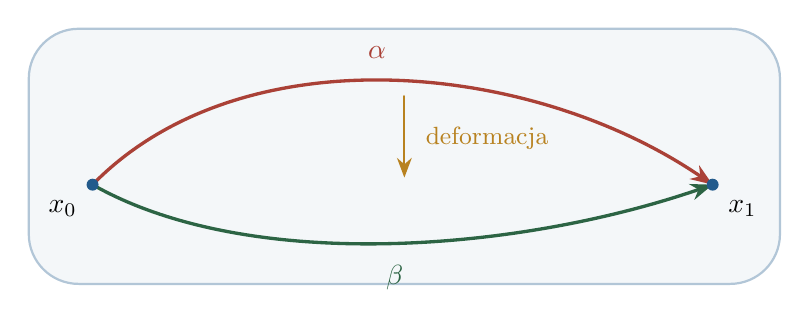
\begin{tikzpicture}[>=Stealth,line cap=round,line join=round,scale=.9]
 \fill[manifoldblue!5,rounded corners=18pt]
  (-.4,-1.15) rectangle (10.2,2.45);
 \draw[manifoldblue!35,thick,rounded corners=18pt]
  (-.4,-1.15) rectangle (10.2,2.45);
 \coordinate (x) at (.5,.25);
 \coordinate (y) at (9.25,.25);
 \draw[manifoldred,very thick,-{Stealth[length=2.8mm]}]
  (x) .. controls (2.6,2.4) and (6.7,2.0) .. (y)
  node[pos=.48,above=4pt] {$\alpha$};
 \draw[manifoldgreen!80!black,very thick,-{Stealth[length=2.8mm]}]
  (x) .. controls (2.7,-1.0) and (6.5,-.7) .. (y)
  node[pos=.51,below=4pt] {$\beta$};
 \draw[manifoldgold!90!black,thick,-{Stealth[length=2.5mm]}]
  (4.9,1.5) -- (4.9,.35)
  node[pos=.52,right=4pt,font=\small] {deformacja};
 \fill[manifoldblue] (x) circle(2.4pt) (y) circle(2.4pt);
 \node[below left=3pt] at (x) {$x_0$};
 \node[below right=3pt] at (y) {$x_1$};
\end{tikzpicture}
\caption{Homotopia dróg przesuwa ich wnętrza,
ale zachowuje oba punkty końcowe.}
\label{fig:homotopia-drog}
\end{figure}

\begin{lemat}[Zmiana prędkości nie zmienia klasy]
\label{lem:reparametr-drogi}
Jeśli $r:I\to I$ jest ciągła, niemalejąca
i spełnia $r(0)=0$, $r(1)=1$, to
$\alpha\circ r$ jest homotopijna z $\alpha$
względem końców.
\end{lemat}
\begin{proof}
Połóżmy $r_t(s)=(1-t)r(s)+ts$.
Każde $r_t$ jest ciągłe, ma te same końce
i wartości w $I$. Funkcja
$H(s,t)=\alpha(r_t(s))$ jest ciągła.
Dla $t=0$ daje $\alpha\circ r$, dla $t=1$
daje $\alpha$, a końce pozostają stałe.
\end{proof}

\begin{twierdzenie}[Grupa podstawowa]
\label{thm:grupa-podstawowa}
Klasy homotopii pętli opartych w $x_0$,
z działaniem $[\alpha][\beta]=[\alpha*\beta]$,
tworzą grupę $\pi_1(X,x_0)$.
Element neutralny to stała pętla $c_{x_0}$,
a odwrotnością $[\alpha]$ jest $[\bar\alpha]$.
\end{twierdzenie}
\begin{proof}
Jeśli $H$ deformuje $\alpha$ w $\alpha'$,
a $K$ deformuje $\beta$ w $\beta'$
względem końców, sklejenie
\[
 L(s,t)=
 \begin{cases}
   H(2s,t),&s\leq\tfrac12,\\
   K(2s-1,t),&s\geq\tfrac12
 \end{cases}
\]
jest ciągłe, bo na wspólnej krawędzi
obie części mają wartość $x_0$.
Działanie nie zależy więc od reprezentantów.

Przy trzech pętlach $(\alpha*\beta)*\gamma$
przeznacza na $\alpha,\beta,\gamma$
odcinki czasu długości $1/4,1/4,1/2$,
zaś $\alpha*(\beta*\gamma)$ długości
$1/2,1/4,1/4$. Obie drogi przebiegają
te same kawałki w tej samej kolejności
i różnią się zmianą parametru.
Lemat~\ref{lem:reparametr-drogi} daje łączność
na klasach. Pętle $c_{x_0}*\alpha$
i $\alpha*c_{x_0}$ różnią się od $\alpha$
tylko chwilą postoju, więc
$[c_{x_0}]$ jest neutralny.

Dla odwrotności określmy
\[
 H(s,t)=
 \begin{cases}
  \alpha(2(1-t)s),&0\leq s\leq\tfrac12,\\
  \alpha(2(1-t)(1-s)),&\tfrac12\leq s\leq1.
 \end{cases}
\]
Przy $s=1/2$ obie gałęzie są równe
$\alpha(1-t)$, a przy $s=0,1$ mają
wartość $x_0$. Jest to homotopia
$\alpha*\bar\alpha$ do pętli stałej
względem punktu bazowego. Zamiana
$\alpha$ z $\bar\alpha$ daje też
$[\bar\alpha][\alpha]=[c_{x_0}]$.
\end{proof}

\begin{stwierdzenie}[Odwzorowania indukowane i punkt bazowy]
\label{prop:pi1-funktor}
Odwzorowanie ciągłe $f:(X,x_0)\to(Y,y_0)$
z $f(x_0)=y_0$ wyznacza homomorfizm
\[
 f_*:\pi_1(X,x_0)\to\pi_1(Y,y_0),
 \qquad [\alpha]\mapsto[f\circ\alpha].
\]
Zachodzi $(gf)_*=g_*f_*$ i
$(\id_X)_*=\id$. Homotopia odwzorowań
utrzymująca $x_0$ w $y_0$ daje
równe homomorfizmy. Jeśli
$u$ jest drogą od $x_0$ do $x_1$,
to $b_u([\alpha])=[\bar u*\alpha*u]$
jest izomorfizmem
$\pi_1(X,x_0)\to\pi_1(X,x_1)$.
\end{stwierdzenie}
\begin{proof}
Złożenie $f\circ H$ przenosi homotopię
pętli w homotopię ich obrazów, a
$f\circ(\alpha*\beta)
=(f\circ\alpha)*(f\circ\beta)$.
Równości dla złożeń wynikają stąd wprost.
Jeśli $F$ jest homotopią odwzorowań utrzymującą
punkt bazowy, $F(\alpha(s),t)$ jest
homotopią pętli opartych w $y_0$.
Wreszcie $b_u$ zachowuje iloczyn:
w środku złożenia pojawia się
$u*\bar u$, homotopijna z pętlą stałą.
Odwrotność stanowi $b_{\bar u}$.
\end{proof}

\begin{wniosek}[Niezmienniczość grupy podstawowej]
\label{cor:pi1-homotopia}
Jeśli $f\simeq g:X\to Y$ przez homotopię
$H$, a $u(t)=H(x_0,t)$ prowadzi od
$f(x_0)$ do $g(x_0)$, to
$g_*=b_u\circ f_*$. Każda równoważność
homotopijna $f:X\to Y$ daje więc
izomorfizm grup podstawowych,
po uwzględnieniu zmiany punktu bazowego.
\end{wniosek}
\begin{proof}
Dla pętli $\alpha$ rozpatrzmy kwadrat
$(s,t)\mapsto H(\alpha(s),t)$.
Jego dolny i górny bok to $f\alpha$
i $g\alpha$, a oba pionowe boki to
$u$. Brzeg kwadratu jest homotopijny do pętli stałej względem
wybranego narożnika: w wypukłym kwadracie ściągamy jego parametryzację
liniowo do tego narożnika, a następnie składamy z $H(\alpha(s),t)$.
Zatem w grupie z punktem
bazowym $g(x_0)$ mamy
$[g\alpha]=[\bar u*(f\alpha)*u]$.
To daje pierwszą równość.

Niech teraz $g$ będzie homotopijną
odwrotnością $f$ i oznaczmy
$y_0=f(x_0)$. Homotopia
$gf\simeq\id_X$ daje drogę $u$
od $gf(x_0)$ do $x_0$ i
izomorfizm $b_u\circ(gf)_*$.
Homotopia $fg\simeq\id_Y$ daje pewną drogę $v$
od $fg(y_0)$ do $y_0$ z $b_v\circ(fg)_*=\id$.
Droga $fu$ ma te same końce, choć może nie być równa $v$.
Ponieważ $b_{fu}\circ b_v^{-1}$ jest izomorfizmem,
również $b_{fu}\circ(fg)_*$ jest izomorfizmem grupy
$\pi_1(Y,y_0)$ na siebie
(każda zmiana punktu bazowego
jest izomorfizmem).
Z naturalności konkatenacji
$f_*\circ b_u=b_{f u}\circ f_*$
na odpowiednich grupach.
Zatem dla $g'_*:=b_u\circ g_*$
oba złożenia $g'_*f_*$
oraz $f_*g'_*$ są izomorfizmami.
Pierwsze zapewnia iniektywność
$f_*$, drugie jego surjektywność.
\end{proof}

Silna retrakcja deformacyjna
z~\ref{def:retrakt-deformacyjny} daje
izomorfizm grup podstawowych w punktach
podprzestrzeni. Dla przestrzeni wypukłej
każdą pętlę $\alpha$ można deformować
wzorem $(1-t)\alpha(s)+tx_0$ do pętli
stałej, nie ruszając punktu bazowego.

\section{Nakrycia: lokalnie wiele kopii jednej przestrzeni}
\label{sec:nakrycia}

Nakrycie przypomina nałożenie kilku arkuszy
na tę samą małą okolicę. Gdy idziemy po bazie,
wybranie początkowego arkusza jednoznacznie
ustala przebieg drogi na nakryciu.
Po zamkniętej drodze możemy wrócić na inny arkusz.

\begin{definicja}[Nakrycie i arkusze]
\index{nakrycie i arkusze@Nakrycie i arkusze}
\label{def:nakrycie}
Surjekcja ciągła $p:E\to X$ jest \emph{nakryciem},
jeśli każdy $x\in X$ ma otwarte otoczenie $U$
takie, że
\[
 p^{-1}(U)=\coprod_{\lambda\in\Lambda}V_\lambda,
 \qquad
 p|_{V_\lambda}:V_\lambda\xrightarrow{\cong}U,
\]
gdzie $V_\lambda$ są parami rozłącznymi
otwartymi podzbiorami $E$, a ograniczenia $p|_{V_\lambda}$
są homeomorfizmami.
Takie $U$ nazywamy \emph{równomiernie nakrytym},
a $V_\lambda$ \emph{arkuszami}.
Włókno $p^{-1}(x)$ jest dyskretne.
\end{definicja}

\begin{przyklad}[Prosta nad okręgiem]
\label{prz:exp-nakrycie}
Odwzorowanie
\[
 p:\R\to S^1,\qquad p(t)=e^{2\pi i t},
\]
jest nakryciem. Jeśli $U$ jest krótkim,
otwartym łukiem okręgu, wybierzmy przedział
$J$ długości mniejszej niż $1$, na którym
$p|_J$ jest homeomorfizmem na $U$.
Wtedy $p^{-1}(U)=\coprod_{k\in\Z}(J+k)$.
Włókno nad $1$ to $\Z$.
Podobnie $q_m:S^1\to S^1$, $q_m(z)=z^m$,
jest $m$-krotnym nakryciem dla $m\geq1$.
Dwukrotne nakrycie $\operatorname{Spin}(n)
\to\mathrm{SO}(n)$ pojawiło się już w
Twierdzeniu~\ref{thm:spin-nakrycie}.
\end{przyklad}

\begin{figure}[!htbp]
\centering
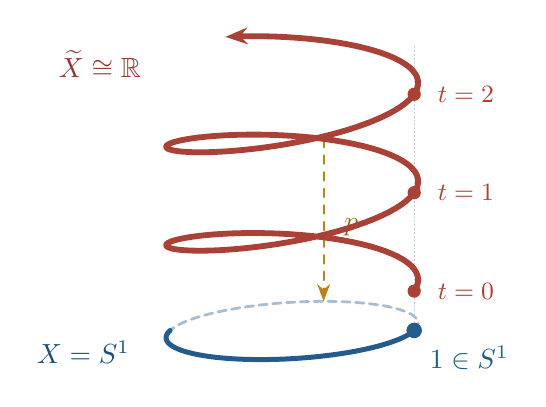
\begin{tikzpicture}[>=Stealth,line cap=round,line join=round,
 x={(1.55cm,0cm)},y={(.40cm,.37cm)},z={(0cm,1.25cm)}]
 % Okrąg u dołu, widoczna i zasłonięta połowa.
 \draw[manifoldblue!40,densely dashed,line width=1pt]
  plot[domain=0:180,samples=60,variable=\u]
   ({cos(\u)},{sin(\u)},0);
 \draw[manifoldblue,line width=1.8pt]
  plot[domain=180:360,samples=60,variable=\u]
   ({cos(\u)},{sin(\u)},0);
 % Włókno nad 1 oraz promień projekcji dla punktu t=1.25.
 \draw[manifoldblue!30,densely dotted]
  (1,0,0)--(1,0,2.9);
 \draw[manifoldgold!90!black,thick,dashed,
       -{Stealth[length=2.2mm]}]
  (0,1,1.65)--(0,1,0);
 \node[manifoldgold!70!black,right=4pt]
  at (0,1,.75) {$p$};
 % Fragment helisy: jeden obrót podnosi wysokość o jedną jednostkę.
 \draw[manifoldred,line width=2.1pt,
       -{Stealth[length=2.8mm]}]
  plot[domain=0:2.38,samples=180,variable=\t]
   ({cos(360*\t)},{sin(360*\t)},{.4+\t});
 \foreach \k in {0,1,2} {
  \fill[manifoldred] (1,0,{.4+\k}) circle(2.4pt);
  \node[manifoldred,right=5pt,font=\small]
   at (1,0,{.4+\k}) {$t=\k$};
 }
 \fill[manifoldblue] (1,0,0) circle(2.8pt);
 \node[manifoldblue,below right=3pt] at (1,0,0) {$1\in S^1$};
 \node[manifoldred!85!black,left=7pt]
  at (-1,0,2.7) {$\widetilde X\cong\R$};
 \node[manifoldblue!85!black,left=11pt]
  at (-1,0,-.22) {$X=S^1$};
\end{tikzpicture}
\caption{Nakrycie $p:\R\to S^1$, $p(t)=e^{2\pi i t}$,
przedstawione jako linia śrubowa nad okręgiem. Rzut pionowy
odpowiada $p$. Punkty linii śrubowej oznaczone $t=0,1,2$
leżą nad tym samym punktem $1\in S^1$.
Pokazano fragment linii śrubowej, która biegnie dalej
w obie strony.}
\label{fig:nakrycie-okragu}
\end{figure}

W poniższych dowodach użyjemy \emph{liczby Lebesgue'a}:
dla otwartego pokrycia zwartej przestrzeni metrycznej istnieje
$\delta>0$ takie, że każdy niepusty zbiór o średnicy mniejszej
niż $\delta$ leży w jednym elemencie pokrycia.
Oto uzasadnienie. Dla każdego $x$ wybierzmy $\varepsilon_x>0$
tak, aby $B(x,2\varepsilon_x)$ mieściła się w elemencie pokrycia.
Ze zwartości skończenie wiele kul $B(x_i,\varepsilon_{x_i})$
pokrywa przestrzeń. Wystarczy $\delta=\min_i\varepsilon_{x_i}$:
jeśli $y$ należy do jednej z tych mniejszych kul, wszystkie
punkty zbioru zawierającego $y$ i o średnicy $<\delta$
leżą w odpowiadającej jej większej kuli. Stosujemy ten fakt
do odcinka i kwadratu z ich zwykłą metryką.

\begin{twierdzenie}[Podnoszenie drogi i homotopii]
\label{thm:podnoszenie-nakrycie}
Niech $p:E\to X$ będzie nakryciem.
\begin{enumerate}[label=(\alph*),leftmargin=*]
\item Każda droga $\gamma:I\to X$ i wybór
      $e_0\in p^{-1}(\gamma(0))$ wyznaczają
      dokładnie jedną drogę
      $\widetilde\gamma:I\to E$ z
      $\widetilde\gamma(0)=e_0$ i
      $p\widetilde\gamma=\gamma$.
\item Jeśli $H:I\times I\to X$ jest
      homotopią dróg, a $\widetilde H(s,0)$
      jest zadanym podniesieniem $H(s,0)$,
      to istnieje dokładnie jedno ciągłe
      podniesienie $\widetilde H$ całego $H$.
      Gdy $H$ zachowuje końce dróg,
      podniesione końce również są stałe.
\end{enumerate}
\end{twierdzenie}
\begin{proof}
\emph{Droga.} Przeciwobrazy równomiernie
nakrytych otwartych $U$ tworzą otwarte
pokrycie odcinka $I$. Z liczby Lebesgue'a
tego pokrycia wybieramy podział
$0=t_0<\cdots<t_N=1$ tak drobny, aby
każdy obraz $\gamma([t_{j-1},t_j])$
mieścił się w jednym $U_j$.
Arkusz nad $U_1$ zawierający $e_0$
określa na pierwszym przedziale wzór
\[
 \widetilde\gamma(t)
 =(p|_{V_1})^{-1}(\gamma(t)).
\]
W punkcie $t_1$ wybieramy arkusz nad $U_2$
zawierający uzyskany punkt włókna i powtarzamy.
Wzory zgadzają się na końcach przedziałów,
więc sklejają się w drogę ciągłą.
Jeśli dwa podniesienia zgadzają się w pewnej
chwili, to lokalnie leżą w tym samym arkuszu
i są identyczne. Gdy w pewnej chwili
się różnią, leżą nad tym samym punktem
w różnych arkuszach, więc również w małej
okolicy chwili pozostają różne. Zbiór
chwil zgodności jest zatem otwarty
i domknięty w spójnym $I$ oraz
zawiera $0$, co daje jednoznaczność.

\emph{Homotopia.} Pokrycie $I^2$ zbiorami
$H^{-1}(U)$ ma liczbę Lebesgue'a.
Dzielimy kwadrat na skończoną siatkę
małych prostokątów, z których każdy ma
obraz w jednym równomiernie nakrytym $U$.
Na dolnej krawędzi mamy zadaną drogę.
Podnosimy prostokąty kolejno od dołu i
od lewej: na każdym wybieramy arkusz
zawierający już ustalony obraz jego narożnika
i stosujemy $(p|_V)^{-1}\circ H$.
Na wspólnej krawędzi oba wzory są
podniesieniami tej samej drogi i zgadzają
się w narożniku, więc na mocy (a) są równe.
Skończone sklejanie daje ciągłą
$\widetilde H$; lokalna jednoznaczność
na spójnym $I^2$ daje jej jedyność.
Jeśli $H(0,t)$ albo $H(1,t)$ jest stała,
jej podniesienie leży w dyskretnym włóknie,
więc też jest stałe.
\end{proof}

Stąd $p_*:\pi_1(E,e_0)\to\pi_1(X,p(e_0))$
jest iniektywny. Jeśli obraz pętli jest
homotopijny do stałej pętli względem bazy,
podnosimy homotopię od danej pętli w $E$.
Końcowa podniesiona pętla leży w dyskretnym
włóknie i jest stała.

\begin{twierdzenie}[Kryterium podnoszenia odwzorowań]
\label{thm:kryterium-podnoszenia}
Niech $Y$ będzie łukowo spójna i lokalnie
łukowo spójna, $f:Y\to X$ ciągła,
$p:E\to X$ nakryciem, a $p(e_0)=f(y_0)$.
Istnieje ciągła $\widetilde f:Y\to E$
z $p\widetilde f=f$ i
$\widetilde f(y_0)=e_0$ wtedy i tylko wtedy, gdy
\[
 f_*\pi_1(Y,y_0)\subseteq
 p_*\pi_1(E,e_0).
\]
Takie podniesienie jest jedyne.
\end{twierdzenie}
\begin{proof}
Gdy $\widetilde f$ istnieje,
$f=p\widetilde f$, zatem
$f_*=p_*\widetilde f_*$, co daje konieczność.
Załóżmy inkluzję. Dla $y\in Y$ wybierzmy
drogę $\gamma$ od $y_0$ do $y$ i
zdefiniujmy $\widetilde f(y)$ jako koniec
podniesienia $f\circ\gamma$ z początkiem $e_0$.
Gdy $\gamma'$ jest innym wyborem,
pętla $f\circ(\gamma'*\bar\gamma)$
ma klasę w obrazie $p_*$. Jest więc
homotopijna względem punktu bazowego
do obrazu pewnej pętli w $E$ o początku
$e_0$. Podnosząc tę homotopię za pomocą
Twierdzenia~\ref{thm:podnoszenie-nakrycie},
otrzymujemy, że podniesienie
$f\circ(\gamma'*\bar\gamma)$ wraca do $e_0$.
Druga część tego zamkniętego podniesienia jest podniesieniem
$f\circ\bar\gamma$ kończącym się w $e_0$.
Po odwróceniu jest, z jednoznaczności, podniesieniem
$f\circ\gamma$ zaczynającym się w $e_0$.
Podniesienia $f\circ\gamma$ i $f\circ\gamma'$ mają więc ten sam koniec.

Sprawdźmy ciągłość, której nie daje sama
definicja punkt po punkcie. Wybierzmy
równomiernie nakryte $U$ zawierające $f(y)$
oraz łukowo spójne otwarte $W\ni y$ z
$f(W)\subseteq U$. Niech $V$ będzie
arkuszem nad $U$ zawierającym $\widetilde f(y)$.
Dla $z\in W$ połączmy $y$ z $z$ drogą
w $W$ i dopiszmy ją do drogi od $y_0$
do $y$. Definicja i podnoszenie drogi
pokazują wtedy, że
$\widetilde f(z)=(p|_V)^{-1}(f(z))$.
Na $W$ odwzorowanie jest więc ciągłe.
Jedyność wynika z jedyności podniesienia
każdej drogi od $y_0$.
\end{proof}

\begin{twierdzenie}[Grupa podstawowa okręgu]
\label{thm:pi1-okragu}
Podnoszenie względem $p:\R\to S^1$
z Przykładu~\ref{prz:exp-nakrycie} daje
izomorfizm
\[
 \operatorname{wind}:\pi_1(S^1,1)\xrightarrow{\ \cong\ }\Z,
 \qquad [\gamma]\longmapsto
 \widetilde\gamma(1),
 \quad \widetilde\gamma(0)=0.
\]
Liczba po prawej to \emph{liczba owinięć}.
\end{twierdzenie}
\begin{proof}
Ponieważ $\gamma(1)=1$, koniec
podniesienia leży w $p^{-1}(1)=\Z$.
Homotopijne pętle dają homotopię
podniesień z nieruchomymi końcami,
więc liczba zależy tylko od klasy.
Jeśli podniesienie $\alpha$ kończy się w $k$,
to podniesienie następnej pętli $\beta$
zaczynające się w $k$ jest przesunięciem
o $k$ podniesienia zaczynającego się w $0$.
Stąd $\operatorname{wind}([\alpha*\beta])
=\operatorname{wind}([\alpha])
+\operatorname{wind}([\beta])$.
Pętla $\gamma_k(s)=e^{2\pi i ks}$
ma podniesienie $ks$, więc homomorfizm
jest surjektywny. Gdy podniesienie
$\widetilde\gamma$ wraca do $0$,
wzór $(s,t)\mapsto(1-t)\widetilde\gamma(s)$
deformuje ją w $\R$ do stałej drogi
z zachowaniem końców. Projekcja tej
homotopii do $S^1$ deformuje $\gamma$
do pętli stałej. Jądro jest zerowe.
\end{proof}

Z Przykładu~\ref{prz:retrakcja-pierscien}
otrzymujemy $\pi_1(\R^2\setminus\{0\})\cong\Z$.
W szczególności okrąg i punkt nie są
homotopijnie równoważne. Obliczenie
$\pi_1(S^{n})=0$ dla $n\geq2$
wyniknie niżej z twierdzenia van Kampena.

\begin{definicja}[Lokalna spójność i warunek półlokalny]
\index{lokalna spojnosc i warunek pollokalny@Lokalna spójność i warunek półlokalny}
\label{def:semilokalnie-prosto-spojna}
Przestrzeń $X$ jest \emph{lokalnie łukowo spójna},
gdy każdy punkt ma bazę otoczeń otwartych,
które są łukowo spójne. Jest
\emph{półlokalnie jednospójna}, gdy każdy
$x\in X$ ma otoczenie $U$, w którym
każda pętla oparta w $x$ jest homotopijna do stałej
względem punktu bazowego \emph{w całym $X$}. Nie wymagamy, aby
ta homotopia mieściła się w $U$.
Przestrzeń łukowo spójna z
$\pi_1(X,x_0)=0$ jest \emph{jednospójna}.
\end{definicja}

Każda rozmaitość topologiczna spełnia
lokalne warunki z tej definicji, gdyż
w otwartej mapie współrzędnych można
wybrać małą kulę. Warunek półlokalny
jest ważny: bez niego nakrycie uniwersalne
może w ogóle nie istnieć.

\begin{twierdzenie}[Konstrukcja nakrycia uniwersalnego]
\label{thm:uniwersalne-nakrycie}
Jeśli $X$ jest łukowo spójna, lokalnie
łukowo spójna i półlokalnie jednospójna,
to ma nakrycie $q:\widetilde X\to X$
z jednospójną przestrzenią $\widetilde X$.
\end{twierdzenie}
\begin{proof}
Ustalmy $x_0\in X$. Punktem $\widetilde X$
niech będzie klasa $[\gamma]$ drogi w $X$
zaczynającej się w $x_0$, przy czym
homotopie zachowują oba końce.
Definiujemy $q([\gamma])=\gamma(1)$.
Istnieje baza otwartych łukowo spójnych
zbiorów $U\subseteq X$, w których
każda pętla jest zerowa po włączeniu do $X$:
najpierw wybieramy otoczenie z warunku
półlokalnego, następnie w nim małe
łukowo spójne otoczenie z lokalnej
łukowej spójności. Każdą pętlę opartą w innym punkcie
takiego $U$ przenosimy do jego wyróżnionego punktu drogą w $U$;
izomorfizm zmiany punktu bazowego pokazuje, że ona też jest zerowa w $X$.

Dla drogi $\gamma$ kończącej się w $x\in U$
niech $W([\gamma],U)$ składa się z klas
$[\gamma*\eta]$, gdzie $\eta$ jest drogą
w $U$ od $x$ do dowolnego $y\in U$.
Jeśli dwie takie drogi $\eta,\eta'$
mają ten sam koniec, to
$\eta*\bar\eta'$ jest pętlą w $U$,
zerową w $X$. Zatem $[\gamma*\eta]
=[\gamma*\eta']$. Otrzymujemy bijekcję
$q:W([\gamma],U)\to U$. Bierzemy wszystkie
te zbiory jako bazę topologii. Sprawdźmy warunek przecięć:
jeśli $[\beta]\in W([\gamma],U)\cap W([\gamma'],U')$,
wybieramy otwarte łukowo spójne $O$ z naszej bazy,
zawierające $\beta(1)$ i zawarte w $U\cap U'$.
Wtedy $W([\beta],O)$ zawiera $[\beta]$ i mieści się w obu zbiorach:
do drogi kończącej się w $\beta(1)$ dopisujemy tylko drogę w $O$.
To dowodzi, że rzeczywiście otrzymujemy bazę.
Ograniczenie $q$ do każdego $W$ jest ciągłe, ponieważ przeciwobrazy
otwartych podzbiorów $U$ są sumami takich mniejszych zbiorów bazowych;
jest też otwarte, bo mniejsze $W([\beta],O)$ przechodzą na otwarte $O$.
Wcześniej wykazana bijekcja jest więc homeomorfizmem.
Jeśli dwa $W$ nad tym samym
$U$ mają wspólny punkt, ich drogi początkowe
różnią się drogą w $U$ z dokładnością
do homotopii w $X$, więc zbiory $W$
są równe. Dla mniejszych otoczeń
używamy ograniczenia tych samych odwzorowań.
Stąd $q^{-1}(U)$ jest rozłączną sumą
arkuszy $W([\gamma],U)$: $q$ jest nakryciem.

Jest ono łukowo spójne. Drogę od klasy
stałej $[c_{x_0}]$ do $[\gamma]$
otrzymujemy, biorąc po kolei klasy
odcinków $\gamma|_{[0,t]}$ po
przeparametryzowaniu na $I$; lokalnie
leżą one w jednym $W$, więc tworzą
ciągłą drogę. Jeśli pętla
$\lambda$ w $\widetilde X$ jest oparta
w $[c_{x_0}]$, jej rzut $\gamma=q\lambda$
ma podniesienie $\lambda$ i kończy
się w tej samej klasie drogi.
Konstrukcja podniesienia pokazuje,
że ta klasa jest $[\gamma]$, więc
$\gamma$ jest homotopijna do stałej
pętli względem bazowego końca.
Podnosimy tę homotopię, zaczynając
od $\lambda$, za pomocą
Twierdzenia~\ref{thm:podnoszenie-nakrycie}.
Na końcu dostajemy stałą pętlę
w dyskretnym włóknie. Zatem
$\pi_1(\widetilde X)=0$.
\end{proof}

\begin{uwaga}[Skąd podgrupy grupy podstawowej?]
\label{uwaga:nakrycia-podgrupy}
Dla spójnego nakrycia $p:(E,e_0)\to(X,x_0)$
iniekcja $p_*$ wyróżnia podgrupę
$H=p_*\pi_1(E,e_0)\leq\pi_1(X,x_0)$.
W warunkach Twierdzenia~\ref{thm:uniwersalne-nakrycie}
każda taka podgrupa daje nakrycie:
na klasach dróg w $\widetilde X$ grupa
$\pi_1(X,x_0)$ działa przez
$[\omega]\cdot[\gamma]=[\omega*\gamma]$,
a iloraz $H\backslash\widetilde X$
jest nakryciem $X$. Istotnie, działanie przenosi
$W([\gamma],U)$ na $W([\omega*\gamma],U)$,
więc jest działaniem przez homeomorfizmy. Jest wolne:
z $[\omega*\gamma]=[\gamma]$ po dopisaniu $\bar\gamma$
wynika $[\omega]=1$.
Co więcej, jeśli $hW\cap W\ne\varnothing$, to $hW=W$,
bo są to arkusze nad tym samym $U$. Ponieważ $q$ jest
iniektywne na $W$ i $q(hz)=q(z)$, element $h$ ustala punkt $z\in W$;
stąd $h=1$. Różne przesunięcia jednego arkusza są więc rozłączne.
Projekcja na orbity jest otwarta: przeciwobraz obrazu zbioru
otwartego $O$ jest sumą otwartych zbiorów $hO$.
Obrazy arkuszy w ilorazie są zatem otwarte i każdy odwzorowuje się
homeomorficznie na $U$. To uzasadnia własność nakrycia.
Przestrzeń ilorazowa jest łukowo spójna jako obraz $\widetilde X$.
Podniesienie pętli $\gamma$ z $x_0$ kończy się w orbicie $[\gamma]$;
wraca do orbity drogi stałej dokładnie wtedy, gdy $[\gamma]\in H$.
Ponieważ obraz homomorfizmu indukowanego przez nakrycie składa się
właśnie z klas mających zamknięte podniesienie, skonstruowane nakrycie
realizuje dokładnie podgrupę $H$.
Z drugiej strony kryterium
\ref{thm:kryterium-podnoszenia} podnosi
$q:\widetilde X\to X$ do $E$, z ustaloną wartością $e_0$.
Przy obecnych założeniach $E$ jest lokalnie łukowo spójna,
więc jej spójność daje łukową spójność: składowe łukowe są otwarte.
Każdy punkt $E$ można połączyć z $e_0$ drogą; rzut tej drogi
pokazuje, że podniesione odwzorowanie $\widetilde X\to E$ jest surjektywne.
Dwa punkty $[\gamma],[\gamma']$ nad tym samym punktem $X$
trafiają w ten sam punkt $E$
dokładnie wtedy, gdy $[\gamma'*\bar\gamma]\in H$.
W jedną stronę składamy podniesione drogi o wspólnym końcu,
otrzymując pętlę w $E$; w drugą używamy podnoszenia homotopii
jak w dowodzie kryterium podnoszenia. Ten warunek jest też
równoważny przynależności do jednej orbity, gdyż
$[\gamma'*\bar\gamma]\cdot[\gamma]=[\gamma']$.
Lokalnie obie projekcje są
homeomorfizmami na $U$, co daje
$E\cong H\backslash\widetilde X$
nad $X$. Zmiana wybranego punktu
$e_0$ sprzęga podgrupę $H$: droga w $E$ między dwoma punktami
nad $x_0$ rzutuje się na pętlę $u$, a zmiana bazy zastępuje
$H$ podgrupą $[\bar u]H[u]$.
Odwrotnie, dowolną pętlę $u$ w $X$ można podnieść z $e_0$;
jej koniec wybiera punkt włókna realizujący właśnie to sprzężenie.
Tak powstaje klasyfikacja spójnych
nakryć przez klasy sprzężoności
podgrup $\pi_1(X,x_0)$.
\end{uwaga}

\section{Twierdzenie van Kampena i pierwsze obliczenia}
\label{sec:van-kampen}

Nakrycie okręgu mierzy jedną liczbę owinięć.
Gdy przestrzeń składa się z kilku części,
potrzebujemy sposobu łączenia informacji
o pętlach w tych częściach.

\begin{twierdzenie}[van Kampen: dwa otwarte zbiory]
\label{thm:van-kampen}
Niech $X=U\cup V$, gdzie $U,V$ są otwarte,
łukowo spójne, a $U\cap V$ jest łukowo
spójne i zawiera $x_0$. Jeśli
$G_U=\pi_1(U,x_0)$, $G_V=\pi_1(V,x_0)$
oraz $G_0=\pi_1(U\cap V,x_0)$, a
$i_U:U\cap V\hookrightarrow U$ i $i_V:U\cap V\hookrightarrow V$
są inkluzjami, to
\[
 \pi_1(X,x_0)\cong
 (G_U*G_V)/
 \left\langle\!\left\langle
 (i_U)_*(h)(i_V)_*(h)^{-1}:h\in G_0
 \right\rangle\!\right\rangle.
\]
Iloczyn wolny wprowadziliśmy w Definicji~\ref{def:free-groups-5};
postać normalną i własność uniwersalną uzasadnia
Stwierdzenie~\ref{prop:free-product-normal-5}. Zapis
$\langle\!\langle\cdot\rangle\!\rangle$
oznacza domknięcie normalne z
Definicji~\ref{def:normal-quotient-5}.
\end{twierdzenie}
\begin{proof}
Inkluzje $U,V\hookrightarrow X$, przez własność uniwersalną
iloczynu wolnego, określają homomorfizm
$\Phi:G_U*G_V\to\pi_1(X,x_0)$.
Pętla w $U\cap V$ daje ten sam obraz
niezależnie od wyboru strony.
Zatem wszystkie relacje z tezy
leżą w $\ker\Phi$.

\emph{Surjektywność.} Dla pętli
$\alpha:I\to X$ przeciwobrazy $U,V$
pokrywają zwarty odcinek. Dzielimy
go na tyle małych przedziałów,
aby obraz każdego leżał w $U$ albo $V$.
Sąsiednie kawałki przypisane temu
samemu zbiorowi łączymy. Każdy
punkt przejścia między kawałkiem
w $U$ i kawałkiem w $V$ leży w
$U\cap V$. Łączymy go z $x_0$
pomocniczą drogą w $U\cap V$.
Jeśli $\lambda_j$ prowadzi od $x_0$
do $j$-tego punktu przejścia,
to z kawałka $\alpha_j$ budujemy
pętlę $\lambda_{j-1}*\alpha_j*
\bar\lambda_j$ całkowicie w $U$
albo w $V$. Iloczyn tych pętli
odtwarza $\alpha$: sąsiednie
$\bar\lambda_j*\lambda_j$
kasują się na mocy
Twierdzenia~\ref{thm:grupa-podstawowa}.

Zmiana drogi $\lambda_j$ na $\lambda'_j$
wyznacza pętlę $h=\lambda'_j*\bar\lambda_j$ w $U\cap V$
\emph{opartą w $x_0$}. Poprzedni czynnik słowa mnożymy z prawej
przez $h^{-1}$, a następny z lewej przez $h$.
Oba zapisy $h$ są równe w ilorazie z tezy, więc się skracają.
Również dopisanie podziału wewnątrz
jednego otwartego zbioru nie zmienia
otrzymanej klasy słowa.

\emph{Jądro.} Przypuśćmy, że słowo
z $G_U*G_V$ daje pętlę homotopijną
do stałej w $X$. Wypełnijmy ją
homotopią $F:I^2\to X$, stałą na
pozostałych trzech bokach.
Zwartość kwadratu pozwala wybrać
siatkę tak drobną, by obraz
każdego małego prostokąta leżał
w całości w $U$ lub w $V$.
Podział dolnego boku dobieramy także tak, aby zawierał końce
pętli reprezentujących litery wyjściowego słowa.
Dla każdego wierzchołka $z$ siatki wybierzmy drogę $\mu_z$
od $x_0$ do $F(z)$. Jeśli $F(z)\in U\cap V$, wybieramy ją
w przecięciu; jeśli $F(z)$ należy tylko do jednego zbioru,
wybieramy drogę w tym zbiorze. Jest to możliwe dzięki założeniom
o łukowej spójności. Przy $F(z)=x_0$ wybieramy drogę stałą.

Zorientowanej krawędzi $e:z\to w$ przypisujemy klasę
$[\mu_z*(F|_e)*\bar\mu_w]$ w grupie zbioru zawierającego
obraz sąsiedniego prostokąta. Obie drogi pomocnicze leżą w tym
zbiorze. Jeżeli dwa sąsiednie prostokąty mają różne oznaczenia,
ich wspólna krawędź i obie drogi pomocnicze leżą w $U\cap V$,
więc przypisania dają ten sam element ilorazu z tezy.
Odwrócenie krawędzi daje element odwrotny.

Iloczyn czterech elementów wokół jednego prostokąta jest jedynką:
drogi pomocnicze skracają się parami, a jego brzeg jest homotopijny
do stałej we właściwym $U$ lub $V$, przez mapę $F$ na tym prostokącie.
Możemy zatem zastępować dwa kolejne boki prostokąta pozostałymi
dwoma, z tymi samymi końcami, bez zmiany elementu ilorazu.
Przesuwając tak łamaną po kolejnych prostokątach, wiersz po wierszu,
zamieniamy dolny bok kwadratu na drogę wzdłuż pozostałych trzech boków.
Te trzy boki są stałe. Na dolnym boku drogi pomocnicze wewnątrz
każdej pierwotnej litery skracają się w jej grupie, a przy końcach
liter są stałe. Odtwarzamy więc dokładnie wyjściowe słowo,
które okazało się jedynką w ilorazie. Każdy krok używał tylko
relacji wewnątrz obu grup i relacji pochodzących z przecięcia.
Stąd $\ker\Phi$ zawiera się we wskazanym domknięciu normalnym
relacji $N$; przeciwna inkluzja wynika z pierwszego kroku,
bo jądro jest podgrupą normalną. Wzór $gN\mapsto\Phi(g)$
jest więc dobrze określonym homomorfizmem na ilorazie.
Jest surjektywny, a jego jądro jest trywialne, ponieważ
$\Phi(g)=1$ zachodzi dokładnie dla $g\in N$. Daje to żądany izomorfizm.
\end{proof}

\begin{przyklad}[Dwa okręgi złączone w punkcie]
\label{prz:pi1-dwa-okregi}
Niech $X=S^1_a\vee S^1_b$.
Wybierzmy na każdym okręgu po jednym
punkcie różnym od punktu sklejenia
$x_0$. Usuwając punkt z drugiego
okręgu, otrzymujemy otwarty $U$
retrakcyjny na $S^1_a$; analogicznie
$V$ retrakcyjny na $S^1_b$.
Przecięcie $U\cap V$ jest ściągalne
(to dwa otwarte łuki spotykające się
w $x_0$). Wobec tego
\[
 \pi_1(S^1\vee S^1,x_0)
 \cong\Z*\Z=:F(a,b).
\]
Słowa $ab$ i $ba$ są różne:
grupa podstawowa nie musi być przemienna.
\end{przyklad}

\begin{przyklad}[Sfera wymiaru co najmniej dwa]
\label{prz:pi1-sfera}
Niech $n\geq2$. Zbiory
$U=S^n\setminus\{N\}$ i
$V=S^n\setminus\{S\}$, gdzie $N,S$
są biegunami, są homeomorficzne
z $\R^n$, więc mają trywialne
grupy podstawowe. Ich przecięcie
jest łukowo spójne: deformuje się
na równik $S^{n-1}$, który jest
łukowo spójny dla $n-1\geq1$.
Twierdzenie~\ref{thm:van-kampen}
daje $\pi_1(S^n)=0$.
Stąd $\pi_1(\R^{n+1}\setminus\{0\})=0$
dla $n\geq2$, co odróżnia ten
przypadek od płaszczyzny.
\end{przyklad}

\section{Sympleksy i triangulacje}
\label{sec:sympleksy}

Sympleks jest najprostszym wielowymiarowym
klockiem: odcinek w wymiarze $1$, trójkąt
w wymiarze $2$, czworościan w wymiarze $3$.
Współrzędne barycentryczne opisują
zarazem punkt i to, na której ścianie leży.

\begin{definicja}[Sympleks standardowy i ściany]
\index{sympleks standardowy i sciany@Sympleks standardowy i ściany}
\label{def:sympleks-standardowy}
Dla $n\geq0$ \emph{standardowy $n$-sympleks}
to
\[
 \Delta^n=
 \left\{(t_0,\ldots,t_n)\in\R^{n+1}:
 t_i\geq0,\ \sum_{i=0}^{n}t_i=1\right\}.
\]
Jego wierzchołki to wektory $e_0,\ldots,e_n$.
\emph{Wnętrze} oznacza $t_i>0$ dla wszystkich $i$
(względem afinicznej otoczki sympleksu).
Dla $n\geq1$ \emph{ściana kowymiaru jeden} naprzeciw $e_i$
jest zadana równaniem $t_i=0$ i jest kopią $\Delta^{n-1}$.
Ogólniej ścianę wyznacza dowolny niepusty podzbiór wierzchołków;
jest właściwa, gdy pomija choć jeden z nich.
Suma wszystkich właściwych ścian to $\partial\Delta^n$.
Przy $n=0$ nie ma niepustych właściwych ścian i $\partial\Delta^0=\varnothing$.
Punkty $v_0,\ldots,v_n\in\R^N$
są \emph{afinicznie niezależne}, jeśli
$v_1-v_0,\ldots,v_n-v_0$ są liniowo
niezależne. Ich otoczka wypukła
$[v_0,\ldots,v_n]$ jest
\emph{geometrycznym $n$-sympleksem}.
\end{definicja}

Każdy punkt sympleksu ma postać
$x=\sum_i t_iv_i$. Współczynniki
$t_i$ są jednoznaczne: jeśli
$\sum_i(t_i-s_i)v_i=0$ i obie sumy
współczynników są równe $1$, to
$\sum_{i=1}^n(t_i-s_i)(v_i-v_0)=0$;
afiniczna niezależność wymusza
$t_i=s_i$ dla wszystkich $i$.
W szczególności usunięcie jednego
wierzchołka daje ścianę
o wymiarze $n-1$.

\begin{figure}[!htbp]
\centering
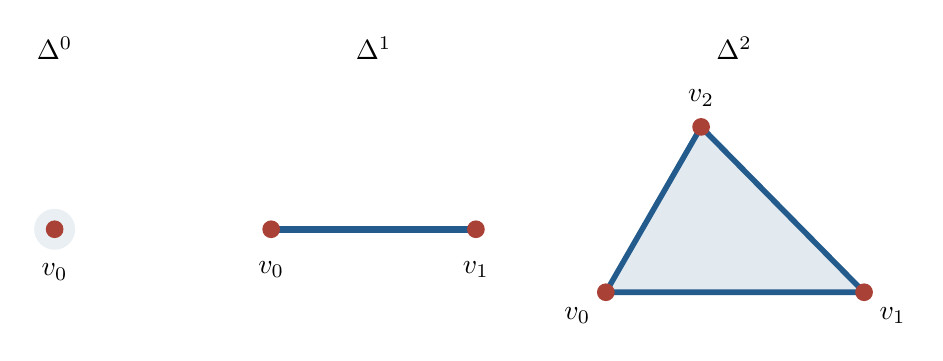
\begin{tikzpicture}[line cap=round,line join=round]
 \node[font=\bfseries] at (0,3.45) {$\Delta^0$};
 \node[font=\bfseries] at (4.05,3.45) {$\Delta^1$};
 \node[font=\bfseries] at (8.63,3.45) {$\Delta^2$};
 % Wymiar zero.
 \fill[manifoldblue!10] (0,1.15) circle(.26);
 \fill[manifoldred] (0,1.15) circle(3.2pt);
 \node[below=9pt] at (0,1.15) {$v_0$};
 % Wymiar jeden.
 \coordinate (b0) at (2.75,1.15);
 \coordinate (b1) at (5.35,1.15);
 \draw[manifoldblue,line width=2.6pt] (b0)--(b1);
 \fill[manifoldred] (b0) circle(3.2pt)
  (b1) circle(3.2pt);
 \node[below=8pt] at (b0) {$v_0$};
 \node[below=8pt] at (b1) {$v_1$};
 % Wymiar dwa.
 \coordinate (c0) at (7.00,.35);
 \coordinate (c1) at (10.28,.35);
 \coordinate (c2) at (8.21,2.45);
 \fill[manifoldblue!13] (c0)--(c1)--(c2)--cycle;
 \draw[manifoldblue,line width=2pt] (c0)--(c1)--(c2)--cycle;
 \fill[manifoldred] (c0) circle(3.2pt)
  (c1) circle(3.2pt) (c2) circle(3.2pt);
 \node[below left=3pt] at (c0) {$v_0$};
 \node[below right=3pt] at (c1) {$v_1$};
 \node[above=4pt] at (c2) {$v_2$};
\end{tikzpicture}
\caption{Sympleksy wymiarów $0,1,2$: punkt,
odcinek i wypełniony trójkąt. Wymiar
$n$ odpowiada $n+1$ afinicznie niezależnym
wierzchołkom; ściany powstają przez ich usunięcie.}
\label{fig:sympleks-trojkat}
\end{figure}

\begin{stwierdzenie}[Brzeg sympleksu jest sferą]
\label{prop:brzeg-sympleksu}
Dla $n\geq1$ przestrzeń $\Delta^n$
jest homeomorficzna z dyskiem $D^n$,
a $\partial\Delta^n$ z $S^{n-1}$.
\end{stwierdzenie}
\begin{proof}
Pracujemy w $n$-wymiarowej płaszczyźnie
afinicznej $P=\{\sum t_i=1\}$.
Środek $c=(1/(n+1),\ldots,1/(n+1))$
leży we wnętrzu. Każdy promień z $c$
w $P$ przecina brzeg dokładnie raz:
nierówności $t_i\geq0$ wyznaczają
na nim odcinek od $c$ do pierwszej
ściany, na której pewna współrzędna
staje się zerem.
Przypisanie punktowi brzegowemu
$x$ kierunku $(x-c)/\|x-c\|$
jest ciągłą bijekcją
$\partial\Delta^n\to S^{n-1}$
po utożsamieniu $P-c\cong\R^n$.
Dziedzina jest zwarta, a sfera
Hausdorffa, więc odwrotność jest
ciągła. Jeśli $b(u)$ jest tą odwrotnością dla kierunku
$u\in S^{n-1}$, wzór $ru\mapsto c+r(b(u)-c)$, $0<r\leq1$,
z wartością $c$ w zerze daje ciągłą bijekcję z $D^n$ na $\Delta^n$.
Ciągłość w zerze wynika z ograniczoności $b(u)-c$.
Ponownie zwartość i własność Hausdorffa dają homeomorfizm,
który na brzegu jest poprzednią identyfikacją. Dla $n=1$ brzeg
składa się z dwóch punktów,
czyli jest $S^0$.
\end{proof}

\begin{definicja}[Skończony kompleks symplicjalny]
\index{skonczony kompleks symplicjalny@Skończony kompleks symplicjalny}
\label{def:kompleks-symplicjalny}
Niech $V$ będzie skończonym zbiorem
wierzchołków. \emph{Kompleks symplicjalny}
$K$ to rodzina niepustych skończonych
podzbiorów $V$ taka, że jeśli
$\sigma\in K$ i $\varnothing\ne\tau\subseteq\sigma$,
to $\tau\in K$. Zbiór o $n+1$
wierzchołkach nazywamy
\emph{$n$-sympleksem} $K$.
Jego \emph{realizacja geometryczna} to
\[
 |K|=\left\{\sum_{v\in V}t_v e_v:
 t_v\geq0,\ \sum_v t_v=1,\
 \{v:t_v>0\}\in K\right\}\subseteq\R^{V}.
\]
Kompleks $L\subseteq K$ zamknięty
na przechodzenie do ścian jest
\emph{podkompleksem}.
\emph{Skończona triangulacja} przestrzeni $X$
to homeomorfizm $|K|\to X$. W tej sekcji ograniczamy się do
skończonych kompleksów; ich realizacje są zwarte. Triangulacje
przestrzeni niezwartych wymagają dopuszczenia nieskończenie wielu sympleksów.
\end{definicja}

W tej definicji dwie różne ściany
mają dokładnie to wspólne, co
wynika ze wspólnych wierzchołków.
Na przykład trzy krawędzie
$[v_0,v_1]$, $[v_1,v_2]$,
$[v_2,v_0]$, bez wnętrza trójkąta,
realizują okrąg. Po dodaniu
$[v_0,v_1,v_2]$ otrzymujemy dysk.
Słowo \emph{podkompleks} jest
ważniejsze niż dowolny podzbiór:
zawiera wraz z sympleksem
wszystkie jego ściany.

\begin{uwaga}[Nie każdy podział na trójkąty
jest kompleksem symplicjalnym]
\label{uwaga:delta-motywacja}
Kwadrat z utożsamionymi przeciwległymi
bokami przedstawia torus. Gdy podzielimy
go jedną przekątną, po sklejeniu wszystkie
cztery narożniki stają się jednym
wierzchołkiem, a każda z dwóch
trójkątnych części nadal ma sens.
Nie jest to \emph{kompleks symplicjalny}
z jednym wierzchołkiem: trójkąt
potrzebuje trzech różnych wierzchołków.
Wygodniejszym opisem są
$\Delta$-kompleksy.
\end{uwaga}

\begin{definicja}[$\Delta$-kompleks]
\label{def:delta-kompleks}
\emph{$\Delta$-kompleks} $X$ jest
przestrzenią Hausdorffa z rodziną ciągłych odwzorowań charakterystycznych
$\sigma_\alpha:\Delta^{n_\alpha}\to X$:
\begin{enumerate}[label=(\roman*),leftmargin=*]
\item ograniczenie $\sigma_\alpha$ do wnętrza
      jest iniektywne, a obrazy wnętrz
      różnych sympleksów są rozłączne
      i pokrywają $X$;
\item ograniczenie $\sigma_\alpha$ do każdej
      ściany jest jednym z odwzorowań
      charakterystycznych niższego wymiaru
      po standardowym afinicznym
      utożsamieniu tej ściany z sympleksem, zachowującym
      kolejność pozostałych wierzchołków;
\item $A\subseteq X$ jest domknięty dokładnie
      wtedy, gdy $\sigma_\alpha^{-1}(A)$
      jest domknięty w każdym
      $\Delta^{n_\alpha}$.
\end{enumerate}
Różne ściany tego samego sympleksu
mogą być tu sklejone, o ile zgodne
są odwzorowania na ich dalszych ścianach.
\end{definicja}

Ostatni warunek to \emph{topologia słaba}
względem odwzorowań charakterystycznych:
odwzorowanie z $X$ do innej przestrzeni
jest ciągłe dokładnie wtedy, gdy jego
złożenia z każdą $\sigma_\alpha$ są ciągłe.
Jest to topologia ilorazowa z
Definicji~\ref{def:topologia-ilorazowa}
na rozłącznej sumie wszystkich sympleksów.

\begin{przyklad}[Okrąg i torus jako $\Delta$-kompleksy]
\label{prz:delta-torus}
Okrąg ma jeden $0$-sympleks $v$
i jeden $1$-sympleks, którego oba końce
przechodzą w $v$. Dla torusa
podzielmy kwadrat $[0,1]^2$
przekątną i sklejmy
$(0,t)\sim(1,t)$ oraz
$(s,0)\sim(s,1)$. Otrzymujemy
jeden wierzchołek, trzy krawędzie
(poziomą $a$, pionową $b$ i przekątną
$c$) oraz dwa $2$-sympleksy. Porządkujemy ich wierzchołki jako
$((0,0),(0,1),(1,1))$ i $((0,0),(1,0),(1,1))$.
Oba porządki nadają krawędziom poziomym kierunek w prawo,
pionowym w górę, a przekątnej kierunek od $(0,0)$ do $(1,1)$.
Mapy ścian są zatem zgodne także z porządkiem wierzchołków.
Iloraz jest homeomorficzny z
$(\R/\Z)\times(\R/\Z)$:
odwzorowanie $(s,t)\mapsto([s],[t])$
identyfikuje dokładnie wskazane
punkty brzegowe, jest ciągłe
i przechodzi na bijekcję
między przestrzenią zwartą
a przestrzenią Hausdorffa.
\end{przyklad}

\begin{figure}[!htbp]
\centering
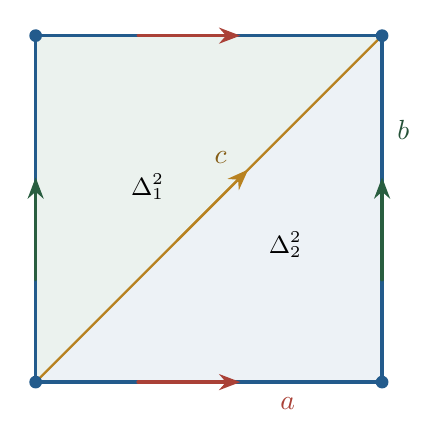
\begin{tikzpicture}[>=Stealth,line cap=round,line join=round,
 x=1cm,y=1cm]
 \coordinate (a) at (0,0);
 \coordinate (b) at (4.4,0);
 \coordinate (c) at (4.4,4.4);
 \coordinate (d) at (0,4.4);
 \fill[manifoldblue!8] (a)--(b)--(c)--cycle;
 \fill[manifoldgreen!10] (a)--(d)--(c)--cycle;
 \draw[manifoldblue,very thick] (a)--(b)--(c)--(d)--cycle;
 \draw[manifoldgold!90!black,thick] (a)--(c);
 \draw[manifoldgold!90!black,thick,-{Stealth[length=2.7mm]}]
  (1.8,1.8)--(2.7,2.7);
 \draw[manifoldred,very thick,-{Stealth[length=2.7mm]}]
  (1.3,0)--(2.6,0);
 \draw[manifoldred,very thick,-{Stealth[length=2.7mm]}]
  (1.3,4.4)--(2.6,4.4);
 \draw[manifoldgreen!75!black,very thick,-{Stealth[length=2.7mm]}]
  (0,1.3)--(0,2.6);
 \draw[manifoldgreen!75!black,very thick,-{Stealth[length=2.7mm]}]
  (4.4,1.3)--(4.4,2.6);
 \node[manifoldred,below=2pt] at (3.2,0) {$a$};
 \node[manifoldgreen!65!black,right=2pt] at (4.4,3.2) {$b$};
 \node[manifoldgold!65!black,above left=2pt]
  at (2.6,2.6) {$c$};
 \foreach \p in {a,b,c,d}
  \fill[manifoldblue] (\p) circle(2.3pt);
 \node[font=\small] at (1.42,2.48) {$\Delta^2_1$};
 \node[font=\small] at (3.17,1.74) {$\Delta^2_2$};
\end{tikzpicture}
\caption{Torus z dwóch sympleksów: boki o tych samych
kolorach i kierunkach sklejamy ze sobą. Przekątna
pozostaje trzecią krawędzią. Wszystkie cztery narożniki
reprezentują ten sam wierzchołek torusa.}
\label{fig:delta-torus}
\end{figure}

\section{Grafy i drzewa}
\label{sec:grafy-drzewa}
\index{graf}
\index{drzewo!grafowe}

Graf $\Gamma=(V,E)$ składa się ze zbioru \emph{wierzchołków}
$V$ i zbioru \emph{krawędzi} $E$, z których każda łączy dwa
różne wierzchołki. Ciąg kolejnych krawędzi to \emph{droga};
jest \emph{prosta}, gdy nie powtarza wierzchołków.
\emph{Cykl} jest zamkniętą drogą bez powtórzeń poza
wspólnym początkiem i końcem. Graf jest \emph{spójny},
jeśli każde dwa wierzchołki łączy droga.

\begin{definicja}[Drzewo, las i korzeń]
\label{def:drzewo-grafowe}
\emph{Drzewo} to spójny graf bez cykli. \emph{Las} to graf
bez cykli, czyli rozłączna suma drzew. W \emph{drzewie
zakorzenionym} wyróżniamy wierzchołek zwany korzeniem;
odległość od niego, liczona liczbą krawędzi jedynej
drogi, jest poziomem wierzchołka. Wierzchołek o jednej
krawędzi nazywamy \emph{liściem}, gdy nie jest korzeniem.
\end{definicja}

Na przykład droga z czterech wierzchołków jest drzewem
o trzech krawędziach, a trójkąt nie jest drzewem, bo
zawiera cykl. W drzewie między dwoma wierzchołkami
istnieje dokładnie jedna droga prosta: spójność daje
istnienie, a dwie różne drogi utworzyłyby cykl.
Jeśli skończone drzewo ma $v$ wierzchołków, ma $v-1$
krawędzi. Dla $v>1$ koniec najdłuższej drogi jest
liściem; po usunięciu tego liścia i jego krawędzi
pozostaje drzewo, więc wzór wynika przez indukcję.
Dla lasu o $c$ składowych ten sam rachunek daje
$|E|=|V|-c$. W drzewach nieskończonych użyjemy
tylko jedyności skończonych dróg; wzór na liczby
wierzchołków i krawędzi dotyczy grafów skończonych.

\section{CW-kompleksy i dołączanie komórek}
\label{sec:cw-kompleksy}

Trójkąty są wygodne do obliczeń, lecz
potrafią wymagać wielu wierzchołków.
Komórka pozwala dołączyć naraz cały
otwarty dysk, przy czym jego brzeg
może biec po starszej części przestrzeni
w sposób nietrywialny.

\begin{definicja}[Dołączenie komórki]
\index{dolaczenie komorki@Dołączenie komórki}
\label{def:dolaczenie-komorki}
Niech $Y$ będzie przestrzenią i
$\varphi:S^{n-1}=\partial D^n\to Y$
odwzorowaniem ciągłym, $n\geq1$.
\emph{Dołączeniem $n$-komórki} jest
przestrzeń ilorazowa
\[
 Y\cup_\varphi D^n
 :=(Y\sqcup D^n)/(z\sim\varphi(z)
 \text{ dla }z\in S^{n-1}).
\]
Obraz wnętrza dysku oznaczamy $e^n$.
Odwzorowanie z dysku do ilorazu jest
\emph{odwzorowaniem charakterystycznym}
tej komórki; $\varphi$ nazywamy
\emph{odwzorowaniem dołączającym}.
W wymiarze $0$ po prostu dołączamy
izolowany punkt, gdyż
$S^{-1}=\varnothing$.
\end{definicja}

Naturalna inkluzja $Y$ w przestrzeń dołączoną jest
homeomorfizmem na domknięty obraz. Dla każdego domkniętego $F\subseteq Y$
przeciwobraz jego obrazu w $Y\sqcup D^n$ jest równy
$F\sqcup\varphi^{-1}(F)$ i jest domknięty; dotyczy to również $F=Y$.
Ponieważ na punktach $Y$ nie wprowadzamy nowych utożsamień,
otrzymujemy to stwierdzenie. Wnętrze $D^n$ jest natomiast
otwartym zbiorem nasyconym, bez żadnych utożsamień, więc przechodzi
homeomorficznie na otwartą komórkę $e^n$.

Topologia ilorazowa z
Definicji~\ref{def:topologia-ilorazowa}
ma tu konkretne znaczenie. Jeśli
$F:Y\cup_\varphi D^n\to Z$
ma być ciągła, wystarczy podać
ciągłe $F_Y:Y\to Z$ i
$F_D:D^n\to Z$ zgodne na brzegu:
$F_D(z)=F_Y(\varphi(z))$.
Istotnie, takie odwzorowania dają ciągłe
odwzorowanie na rozłącznej sumie, stałe
na każdej klasie sklejenia;
uniwersalna własność ilorazu
przenosi je na iloraz.
To jest praktyczny sposób
konstruowania odwzorowań na przestrzeniach
sklejonych.

\begin{definicja}[CW-kompleks]
\index{cw-kompleks@CW-kompleks}
\label{def:cw-kompleks}
\emph{CW-kompleks} $X$ jest przestrzenią Hausdorffa budowaną
ze szkieletów $X^0\subseteq X^1
\subseteq X^2\subseteq\cdots$:
$X^0$ jest dyskretnym zbiorem punktów,
a $X^n$ powstaje z $X^{n-1}$
przez dołączenie rodziny $n$-dysków
odwzorowaniami $S^{n-1}\to X^{n-1}$.
Przestrzeń $X=\bigcup_n X^n$
ma \emph{topologię słabą}:
$A\subseteq X$ jest domknięty,
dokładnie wtedy, gdy przeciwobraz $A$ pod każdym
odwzorowaniem charakterystycznym $D^n\to X$
jest domknięty. Wymagamy ponadto
\emph{skończoności domknięć komórek}:
domknięcie każdej komórki
spotyka tylko skończenie wiele
komórek. Litery CW przypominają
te dwa warunki
(\emph{closure-finite}, \emph{weak topology}).
\emph{Podkompleks CW} to suma komórek
domknięta w $X$; jeśli zawiera komórkę,
zawiera także całe jej domknięcie.
\end{definicja}

\begin{figure}[!htbp]
\centering
\begin{tikzpicture}[>=Stealth,line cap=round,line join=round]
 \node[font=\bfseries] at (0,3.02) {$X^0$};
 \node[font=\bfseries] at (4.33,3.02) {$X^1$};
 \node[font=\bfseries] at (8.68,3.02) {$X^2$};
 % 0-komórka.
 \fill[manifoldred] (0,1.39) circle(3.7pt);
 \node[below=7pt] at (0,1.39) {$e^0=\{v\}$};
 % Dołączenie 1-komórki: oba końce trafiają do v.
 \draw[manifoldblue,line width=2.5pt]
  (4.33,1.45) circle(1.03);
 \fill[manifoldred] (4.33,.42) circle(3.7pt);
 \node[manifoldblue!85!black] at (4.33,1.45) {$e^1$};
 \draw[->,manifoldblue!75!black,thin]
  (4.62,1.74)--({4.33+1.03*cos(45)},{1.45+1.03*sin(45)});
 \node[below=7pt] at (4.33,.42) {$v$};
 \draw[->,manifoldgold!80!black,thick]
  (1.22,1.54)--(3.08,1.54)
  node[midway,above=5pt,font=\small] {dołącz $e^1$};
 % Dołączenie 2-komórki: brzeg dysku biegnie po okręgu.
 \fill[manifoldgreen!18] (8.68,1.45) circle(1.03);
 \draw[manifoldblue,line width=2.5pt]
  (8.68,1.45) circle(1.03);
 \fill[manifoldred] (8.68,.42) circle(3.7pt);
 \node[manifoldgreen!65!black] at (8.68,1.45) {$e^2$};
 \node[below=7pt] at (8.68,.42) {$v$};
 \draw[->,manifoldgold!80!black,thick]
  (5.58,1.54)--(7.35,1.54)
  node[midway,above=5pt,font=\small] {dołącz $e^2$};
\end{tikzpicture}
\caption{Przykłady kolejnych wymiarów CW: punkt
$X^0=\{v\}$, okrąg $X^1\cong S^1$ otrzymany
przez sklejenie obu końców $1$-komórki z $v$,
oraz dysk $X^2\cong D^2$ po dołączeniu
$2$-komórki wzdłuż całego okręgu.
Czerwony punkt, niebieski łuk i zielone wnętrze
oznaczają odpowiednio otwarte komórki
wymiarów $0,1,2$.}
\label{fig:cw-wymiary}
\end{figure}

W kompleksie skończonym warunki
topologiczne łatwo sprawdzić
bez osobnej teorii granic:
topologia słaba jest ilorazową
topologią sklejania skończenie
wielu dysków, a domknięcie
każdej komórki spotyka
tylko skończenie wiele innych.
Przy nieskończenie wielu komórkach
topologia słaba jest konieczna,
aby ciągłość dało się sprawdzać
na wszystkich domkniętych komórkach.

\begin{stwierdzenie}[Sympleksy dają komórki]
\label{prop:sympleksy-cw}
Skończony kompleks symplicjalny i
skończony $\Delta$-kompleks są
CW-kompleksami: ich otwarte komórki
to obrazy wnętrz sympleksów.
\end{stwierdzenie}
\begin{proof}
Indukujemy po wymiarze. Szkielet
zerowy składa się z wierzchołków.
Wnętrze każdego $n$-sympleksu
jest rozłączne z obrazami innych
wnętrz, a brzeg jest sumą ścian
zawartych w poprzednim szkielecie.
Stwierdzenie~\ref{prop:brzeg-sympleksu}
pozwala traktować sympleks
jako dysk $D^n$, którego
odwzorowanie na brzegu jest odwzorowaniem dołączającym.
Warunek o topologii jest w
Definicji~\ref{def:delta-kompleks}
podany wprost, a dla skończonej
realizacji symplicjalnej wynika
z topologii skończonej sumy zwartych sympleksów:
ciągła surjekcja z tej sumy na $|K|\subseteq\R^V$ jest domknięta,
gdyż obrazy zbiorów domkniętych są zwarte w przestrzeni Hausdorffa.
Jest więc odwzorowaniem ilorazowym, co daje właśnie wymaganą topologię.
Skończona liczba sympleksów
zapewnia skończoność domknięć komórek.
\end{proof}

\begin{przyklad}[Minimalne struktury komórkowe]
\label{prz:cw-sfera-torus}
\begin{enumerate}[label=(\arabic*),leftmargin=*]
\item Dla $n\geq1$ sfera $S^n$
      ma jedną $0$-komórkę i jedną
      $n$-komórkę:
      $D^n/S^{n-1}\cong S^n$.
      Jawny homeomorfizm opisujemy
      poniżej.
      Dla $S^0$ używamy dwóch
      $0$-komórek.
\item Torus ma jedną $0$-komórkę,
      dwie $1$-komórki $a,b$ oraz
      jedną $2$-komórkę. Obchodząc
      brzeg kwadratu z
      Rysunku~\ref{fig:delta-torus},
      otrzymujemy słowo
      $aba^{-1}b^{-1}$ w
      $S^1\vee S^1$.
      Dwa trójkąty realizacji
      $\Delta$-kompleksowej zostały
      zastąpione jednym dyskiem,
      którego odwzorowanie dołączające
      zapamiętuje sklejanie.
\end{enumerate}
\end{przyklad}

\begin{przyklad}[Sfera $S^2$ bez $1$-komórek]
\label{prz:cw-s2}
Weźmy $X^0=\{v\}$ i nie dołączajmy
żadnej $1$-komórki, więc $X^1=X^0$.
Niech odwzorowanie dołączające
$\varphi:\partial D^2=S^1\to\{v\}$
będzie stałe. Wtedy
\[
 X^2=X^1\cup_\varphi D^2
 \cong D^2/\partial D^2\cong S^2.
\]
Cały brzeg dysku staje się \emph{jednym}
punktem $v$; obraz jego wnętrza
jest jedną otwartą $2$-komórką
$e^2=S^2\setminus\{v\}\cong\R^2$.
Rysunek~\ref{fig:cw-s2} pokazuje to
sklejenie. W szczególności
$X^1$ nie jest okręgiem:
okrąg po lewej stronie rysunku
to brzeg \emph{dołączanego dysku},
a nie komórka przestrzeni wynikowej.
\end{przyklad}

\begin{figure}[!htbp]
\centering
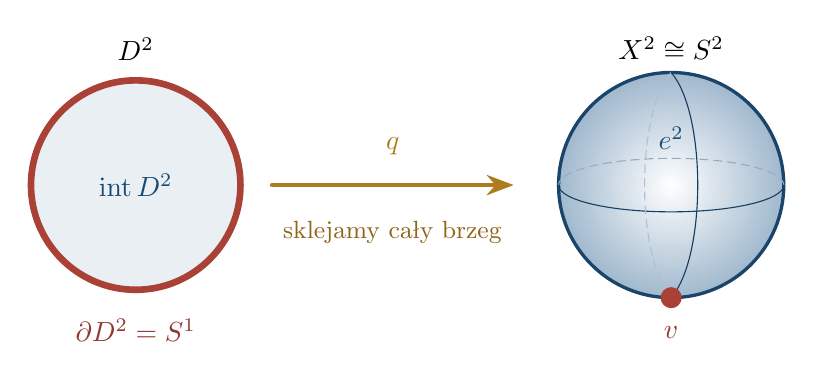
\begin{tikzpicture}[>=Stealth,line cap=round,line join=round]
 % Dysk przed sklejeniem: czerwony brzeg zapada się do v.
 \fill[manifoldblue!10] (0,1.85) circle(1.33);
 \draw[manifoldred,line width=2.4pt] (0,1.85) circle(1.33);
 \node[font=\bfseries] at (0,3.58) {$D^2$};
 \node[manifoldblue!80!black] at (0,1.85) {$\operatorname{int}D^2$};
 \node[manifoldred!85!black,below=7pt]
  at (0,.52) {$\partial D^2=S^1$};
 % Sklejenie brzegu do jednego punktu.
 \draw[->,manifoldgold!85!black,line width=1.5pt]
  (1.73,1.85)--(4.8,1.85)
  node[midway,above=7pt] {$q$};
 \node[font=\small,manifoldgold!70!black]
  at (3.26,1.25) {sklejamy cały brzeg};
 % Sfera w stylistyce rysunku 1.4: jasny środek, tył i przód łuków.
 \shade[inner color=white,outer color=manifoldblue!43]
  (6.8,1.85) circle(1.43);
 \draw[manifoldblue!75!black,very thick]
  (6.8,1.85) circle(1.43);
 \draw[manifoldblue!50,densely dashed,thin]
  (8.23,1.85) arc[start angle=0,end angle=180,x radius=1.43,y radius=.34];
 \draw[manifoldblue!70!black,thin]
  (5.37,1.85) arc[start angle=180,end angle=360,x radius=1.43,y radius=.34];
 \draw[manifoldblue!38,densely dashed,thin]
  (6.8,3.28) .. controls (6.35,2.76) and (6.35,.94) .. (6.8,.42);
 \draw[manifoldblue!65!black,thin]
  (6.8,3.28) .. controls (7.25,2.76) and (7.25,.94) .. (6.8,.42);
 \fill[manifoldred] (6.8,.42) circle(3.8pt);
 \node[font=\bfseries] at (6.8,3.58) {$X^2\cong S^2$};
 \node[manifoldblue!85!black] at (6.8,2.44) {$e^2$};
 \node[manifoldred!85!black,below=7pt] at (6.8,.42) {$v$};
\end{tikzpicture}
\caption{Struktura CW sfery: $D^2$ dołączamy do
punktu $v$ odwzorowaniem stałym na całym brzegu;
$q:D^2\to D^2/\partial D^2$ jest mapą ilorazową.
W powstałej sferze czerwony punkt to
jedyne $e^0$, a cała pozostała powierzchnia
to jedna otwarta komórka $e^2$.
Nie występują komórki wymiaru $1$.}
\label{fig:cw-s2}
\end{figure}

\begin{uwaga}[Uwaga o ilorazie dysku]
W punkcie (1) nie potrzebujemy
identyfikować półkuli z ilorazem
za pomocą niejawnego rysunku.
Istnieje jawne ciągłe odwzorowanie
$D^n\to S^n\subseteq\R^{n+1}$,
\[
 x\longmapsto
 \bigl(\sin(\pi\|x\|)\,x/\|x\|,
       \cos(\pi\|x\|)\bigr)
 \quad(x\ne0),
\]
z wartością $(0,\ldots,0,1)$
w $x=0$. Cały brzeg $\|x\|=1$
przechodzi w biegun południowy,
a na wnętrzu odwzorowanie jest iniektywne
i pokrywa sferę bez tego bieguna.
Przechodzi więc na ciągłą bijekcję
$D^n/S^{n-1}\to S^n$, która jest
homeomorfizmem przez zwartość
dziedziny i własność Hausdorffa
sfery.
\end{uwaga}

\begin{twierdzenie}[Co robi dołączenie komórki z $\pi_1$?]
\label{thm:pi1-dolaczenie-komorki}
Niech $Y$ będzie łukowo spójna,
a $X=Y\cup_\varphi D^n$.
Jeśli $n=2$, po wyborze drogi od
punktu bazowego do $\varphi(S^1)$
grupa $\pi_1(X)$ jest ilorazem
$\pi_1(Y)$ przez domknięcie normalne
klasy pętli $\varphi$.
Jeśli $n\geq3$, włączenie
$Y\hookrightarrow X$ wyznacza
izomorfizm na $\pi_1$.
\end{twierdzenie}
\begin{proof}
W dysku wybierzmy promień $r=\|x\|$.
Otwarty w $X$ zbiór $U$ złożony
z $Y$ i pasa $r>1/3$ deformuje
się na $Y$: przesuwamy punkty
pasa promieniowo do $r=1$,
a punkty $Y$ zostawiamy. Na części dyskowej homotopia ma wzór
$ru\mapsto((1-t)r+t)u$, gdzie $u\in S^{n-1}$.
Wyjaśnijmy ciągłość przy sklejanym $Y$. Dla otwartego otoczenia
$O$ punktu $y\in Y$ zmniejszamy jego część dyskową do punktów $ru$,
dla których $\varphi(u)\in O\cap Y$ i cały odcinek
$\{\rho u:r\leq\rho\leq1\}$ leży w przeciwobrazie $O$.
Ta część jest otwarta: zawieranie zwartego odcinka w zbiorze
otwartym zachowuje się przy małej zmianie $r,u$.
Wraz z $O\cap Y$ tworzy otwarte otoczenie $y$ w ilorazie,
którego obraz przez homotopię pozostaje w $O$ dla wszystkich $t$.
Dowodzi to ciągłości przy $Y$; na wnętrzu dysku wynika ona z podanego wzoru.
Drugi otwarty zbiór $V$ jest
obrazem $r<2/3$; jest to
ściągalne wnętrze dysku.
Przecięcie $U\cap V$ to pierścień
$1/3<r<2/3$, homotopijnie
równoważny $S^{n-1}$.
Jest łukowo spójne dla $n\geq2$.
Otwartość obu zbiorów sprawdzamy przed sklejeniem:
przeciwobrazy $U$ to całe $Y$ i otwarty w $D^n$ pas $r>1/3$,
a przeciwobraz $V$ to $r<2/3$, bez punktów $Y$.

Twierdzenie~\ref{thm:van-kampen}
z $G_V=1$ mówi, że $\pi_1(X)$
jest ilorazem $\pi_1(U)\cong\pi_1(Y)$
przez domknięcie normalne obrazu
$\pi_1(U\cap V)$. Przy $n=2$
generator $\pi_1(S^1)\cong\Z$
po przejściu przez retrakcję
$U\to Y$ staje się pętlą
$\varphi$ (z uwzględnieniem
drogi do punktu bazowego).
Przy $n\geq3$ mamy
$\pi_1(S^{n-1})=0$ z
Przykładu~\ref{prz:pi1-sfera},
więc nie pojawia się żadna
relacja ani nowy generator.
\end{proof}

\begin{przyklad}[Torus i powierzchnia rzutowa]
\label{prz:pi1-torus-rp2}
Dla torusa część jednowymiarowa
jest $S^1\vee S^1$, z grupą
$F(a,b)$ z Przykładu~\ref{prz:pi1-dwa-okregi}.
Dołączona $2$-komórka wymusza
$aba^{-1}b^{-1}=1$, czyli
\[
 \pi_1(T^2)\cong
 \langle a,b\mid ab=ba\rangle
 \cong\Z^2.
\]
Rachunek tej prezentacji przeprowadziliśmy w
Przykładzie~\ref{prz:prezentacja-torusa-5}; dołączenie komórki
uzasadnia teraz topologicznie pochodzenie relacji.
Drugim przykładem jest
$\R P^2$: dysk będący górną
półkulą $S^2$ ma na brzegu
antypody utożsamione, więc
$\R P^2$ ma $0$-komórkę,
      $1$-komórkę i $2$-komórkę
      dołączoną do $S^1\cong\R P^1$
      odwzorowaniem odpowiadającym
      $z\mapsto z^2$ (liczba owinięć wynosi $2$).
      Istotnie, $S^1/(z\sim-z)\to S^1$, $[z]\mapsto z^2$,
      jest homeomorfizmem jako ciągła bijekcja ze zwartej
      przestrzeni do przestrzeni Hausdorffa; odwzorowanie dołączające
      przechodzi przez ten iloraz. Pełny obieg brzegu daje zatem dwa obiegi
      $1$-szkieletu, co wyjaśnia relację $a^2=1$.
      Zatem
\[
 \pi_1(\R P^2)
 \cong\langle a\mid a^2=1\rangle
 \cong\Z/2\Z.
\]
W obu przykładach relacja grupowa pochodzi bezpośrednio
z przebiegu brzegu dołączanej $2$-komórki.
\end{przyklad}

\begin{uwaga}[Granica obecnego rozdziału]
Sympleksy i komórki dają
konkretne przestrzenie, a ich
odwzorowania dołączające kodują sposób
sklejenia. W następnym rozdziale
zorientowanym sympleksom przypiszemy
generatory łańcuchów, a ich ścianom
operator brzegu $\partial$.
Sprawdzimy $\partial^2=0$,
porównamy homologię symplicjalną,
singularną i komórkową oraz
wykorzystamy długie ciągi
z Rozdziału~\ref{ch:algebra-homologiczna}.
Wyższe grupy homotopii i twierdzenie
Hurewicza wymagają już tak
zbudowanej homologii przestrzeni.
\end{uwaga}

\par\smallskip
{\footnotesize\noindent\emph{Dalsza lektura:}
Pełne rozwinięcie teorii homotopii,
nakryć, kompleksów CW i
$\Delta$-kompleksów podaje
Allen Hatcher, \emph{Algebraic Topology},
rozdziały 0 i 1 oraz początek rozdziału 2,
\url{https://pi.math.cornell.edu/~hatcher/AT/AT.pdf}.
W tym rozdziale wyprowadziliśmy
podstawowe własności, które
wykorzystamy do budowania homologii.\par}

\clearpage

\chapter{Homologia przestrzeni}
\label{ch:homologia-przestrzeni}

W Rozdziale~\ref{ch:algebra-homologiczna} homologia była
niezmiennikiem \emph{kompleksu łańcuchowego}.
Teraz przypiszemy taki kompleks przestrzeni. Najpierw
użyjemy sympleksów z Rozdziału~\ref{ch:topologia-algebraiczna-podstawy};
potem zastąpimy je wszystkimi ciągłymi obrazami sympleksów,
aby móc badać przestrzenie bez wybranej triangulacji. Na końcu
zobaczymy, dlaczego do obliczeń zwykle wystarczy
kilka komórek CW.

Intuicja jest jedna: cykl to suma zorientowanych kawałków
bez brzegu, a brzeg to cykl, który ogranicza kawałek
o wymiar wyższy. Iloraz
\[
 H_n(X;\Z)=
 \frac{\{\text{$n$-cykle w $X$}\}}
 {\{\text{brzegi $(n+1)$-łańcuchów w $X$}\}}
\]
odróżnia na przykład pętlę będącą brzegiem na tarczy od pętli
obiegającej dziurę. Pracujemy nad $\Z$; zmianę
współczynników omawia
Twierdzenie~\ref{thm:homologia-char-zero},
a konkretny rachunek znajduje się poniżej.

\section{Łańcuchy symplicjalne: orientacja i brzeg}
\label{sec:homologia-symplicjalna}

\begin{definicja}[Kompleks łańcuchów symplicjalnych]
\index{kompleks lancuchow symplicjalnych@Kompleks łańcuchów symplicjalnych}
\label{def:homologia-symplicjalna}
Niech $K$ będzie skończonym kompleksem symplicjalnym
z Definicji~\ref{def:kompleks-symplicjalny}.
Ustalmy porządek jego wierzchołków. Grupa
$C_n^\Delta(K)$ jest wolną grupą abelową z bazą
wszystkich $n$-sympleksów zapisanych w porządku
$[v_0,\ldots,v_n]$. Jeśli wierzchołki wypiszemy
w innej kolejności, przyjmujemy zasadę
\[
 [v_{\pi(0)},\ldots,v_{\pi(n)}]
 =\operatorname{sgn}(\pi)[v_0,\ldots,v_n].
\]
Zatem odwrócenie orientacji zmienia znak, a dwa
różne sympleksy nadal dają niezależne generatory.
Dla $n\geq1$ określamy
\begin{equation}\label{eq:brzeg-symplicjalny}
 \partial_n[v_0,\ldots,v_n]
 =\sum_{i=0}^n(-1)^i
 [v_0,\ldots,\widehat v_i,\ldots,v_n],
 \qquad \partial_0=0.
\end{equation}
Rozszerzamy $\partial$ liniowo na sumy
o całkowitych współczynnikach. Dla $n<0$ przyjmujemy $C_n^\Delta(K)=0$.
\end{definicja}

Znak ściany nie jest ozdobą: kierunek odziedziczony
przez brzeg wypełnionego trójkąta musi być spójny.
Dla $e=[v_0,v_1]$ i $t=[v_0,v_1,v_2]$ dostajemy
\[
 \partial e=[v_1]-[v_0],\qquad
 \partial t=[v_1,v_2]-[v_0,v_2]+[v_0,v_1].
\]
Drugą równość można zapisać
$\partial t=[v_0,v_1]+[v_1,v_2]+[v_2,v_0]$.
Jest to obieg brzegu trójkąta.

\begin{figure}[!htbp]
\centering
\begin{tikzpicture}[>=Stealth,line cap=round,line join=round]
 \coordinate (a) at (0,0); \coordinate (b) at (3.3,0);
 \coordinate (c) at (1.35,2.55);
 \fill[manifoldblue!13] (a)--(b)--(c)--cycle;
 \draw[manifoldblue!65!black,line width=1.6pt]
  (a)--(b)--(c)--cycle;
 \draw[->,manifoldred,line width=1.5pt]
  (.7,-.13)--(2.5,-.13);
 \draw[->,manifoldred,line width=1.5pt]
  (3.1,.38)--(1.8,2.07);
 \draw[->,manifoldred,line width=1.5pt]
  (1.04,2.1)--(.13,.39);
 \foreach \p in {a,b,c}{\fill[manifoldgold!85!black] (\p) circle(2.8pt);}
 \node[below left] at (a) {$v_0$};
 \node[below right] at (b) {$v_1$};
 \node[above] at (c) {$v_2$};
 \node[manifoldblue!75!black] at (1.4,.84) {$t$};
 \node[align=left,anchor=west,text width=5.5cm] at (4.1,1.38)
  {$\partial t=e_{01}+e_{12}+e_{20}$\\[3pt]
   zewnętrzna pętla jest brzegiem, gdy wnętrze $t$
   należy do przestrzeni};
\end{tikzpicture}
\caption{Zorientowany brzeg trójkąta. Usunięcie jego
wnętrza pozostawia cykl, który w samym okręgu
nie jest już brzegiem żadnego $2$-łańcucha.}
\label{fig:homologia-trojkat}
\end{figure}

\begin{twierdzenie}[Brzeg brzegu znika]
\label{thm:brzeg-brzegu}
Odwzorowania~\eqref{eq:brzeg-symplicjalny}
spełniają $\partial_{n-1}\partial_n=0$.
Wobec tego
\[
 H_n^\Delta(K):=
 \ker(\partial_n:C_n^\Delta(K)\to C_{n-1}^\Delta(K))
 \big/
 \operatorname{im}(\partial_{n+1})
\]
jest dobrze określoną grupą. Licznik składa
się z \emph{cykli}, mianownik z \emph{brzegów}.
\end{twierdzenie}
\begin{proof}
Dla $n=1$ wynika to z $\partial_0=0$.
Niech $n\geq2$ i weźmy generator
$[v_0,\ldots,v_n]$. Każda jego ściana
o wymiarze $n-2$ powstaje po usunięciu
pewnych dwóch wierzchołków $v_i,v_j$,
$i<j$, dokładnie na dwa sposoby.
Usunięcie najpierw $v_i$, a następnie
$v_j$ (ma on już pozycję $j-1$) daje
współczynnik $(-1)^i(-1)^{j-1}$.
W przeciwnej kolejności współczynnik
wynosi $(-1)^j(-1)^i$.
Ich suma to
$(-1)^{i+j-1}+(-1)^{i+j}=0$.
Dotyczy to każdej ściany z osobna,
więc $\partial^2$ znika na bazie,
a przez liniowość na całej grupie.
Stąd $\operatorname{im}\partial_{n+1}
\subseteq\ker\partial_n$, co pozwala
utworzyć podany iloraz.
\end{proof}

\begin{przyklad}[Odcinek, okrąg, tarcza]
\label{prz:homologia-odcinek-okrag}
Odcinek ma dwa wierzchołki $v_0,v_1$
i jedną krawędź $e$. Odwzorowanie
$\partial_1:\Z e\to\Z v_0\oplus\Z v_1$
przypisuje $me\mapsto m(v_1-v_0)$.
Ma zerowe jądro, więc $H_1^\Delta=0$,
a w ilorazie $H_0^\Delta$ obie klasy
wierzchołków są równe. Otrzymujemy $\Z$.

Teraz weźmy obwód trójkąta, bez wnętrza,
i ustawmy kierunki $e_{01},e_{12},e_{20}$.
Każdy $1$-łańcuch
$ae_{01}+be_{12}+ce_{20}$ jest cyklem
dokładnie wtedy, gdy $a=b=c$
(współczynnik przy każdym wierzchołku
w jej brzegu musi być zerem).
Nie ma tu $2$-sympleksów, a więc
$H_1^\Delta\cong\Z$ z generatorem
$e_{01}+e_{12}+e_{20}$.
Jeśli wstawimy wnętrze $t$, ten sam
cykl staje się $\partial t$ i
$H_1^\Delta$ znika. Rysunek~\ref{fig:homologia-trojkat}
pokazuje dokładnie tę zmianę.
\end{przyklad}

W $\Delta$-kompleksie z
Definicji~\ref{def:delta-kompleks} postępujemy
podobnie: każdy \emph{sympleks charakterystyczny}
jest osobnym generatorem, nawet jeżeli jego
różne ściany mają ten sam obraz. Brzeg
jest sumą obrazów ścian z ich znakami;
po identyfikacji mogą się one wzajemnie
skasować. Tak właśnie sklejony odcinek
z jednym wierzchołkiem ma $\partial e=v-v=0$.

\begin{stwierdzenie}[Składowe i $H_0$]
\label{prop:h0-symplicjalne}
Jeżeli $K$ ma $c$ składowych łukowych,
to $H_0^\Delta(K)\cong\Z^c$.
\end{stwierdzenie}
\begin{proof}
Ponieważ $\partial_0=0$, grupa $H_0$
to wolna grupa na wierzchołkach
modulo relacje
$v_j-v_i=\partial[v_i,v_j]$
dla krawędzi. Idąc po drodze krawędziowej,
utożsamiamy klasy wszystkich wierzchołków
jej składowej. Dwa wierzchołki tej samej
składowej $|K|$ można połączyć taką drogą:
wszystkie wierzchołki jednego sympleksu należą do tej samej
składowej grafu krawędzi. Sympleksy przypisane jednej takiej
składowej tworzą podkompleks. Jego realizacja i jej dopełnienie
są domknięte jako skończone sumy domkniętych sympleksów,
więc są też otwarte. Droga nie może przejść między tymi zbiorami.
Każdy punkt sympleksu można natomiast połączyć odcinkiem z wierzchołkiem.
Składowe grafu odpowiadają zatem dokładnie składowym łukowym $|K|$. Wreszcie żadna
relacja nie łączy różnych składowych,
bo obie końcówki każdej krawędzi leżą
w jednej. W każdej składowej pozostaje
więc jeden wolny generator.
\end{proof}

\section{Łańcuchy singularne i niezmienniczość homotopijna}
\label{sec:homologia-singularna}

Triangulacja bywa trudna do znalezienia. W konstrukcji
singularnej sam wybór \emph{ciągłego} odwzorowania
standardowego sympleksu do przestrzeni tworzy
generator; nie żądamy różnowartościowości ani
ładnego kształtu jego obrazu.

\begin{definicja}[Homologia singularna]
\index{homologia singularna@Homologia singularna}
\label{def:homologia-singularna}
\emph{Singularny $n$-sympleks} w $X$ to dowolne
ciągłe odwzorowanie $\sigma:\Delta^n\to X$.
Niech $C_n(X)$ będzie wolną grupą abelową
na wszystkich takich odwzorowaniach; dla $n<0$ przyjmujemy $C_n(X)=0$.
W szczególności
dwa różne odwzorowania o tym samym obrazie są
różnymi generatorami. Niech
$\iota_i:\Delta^{n-1}\to\Delta^n$
będzie afinicznym włączeniem ściany
naprzeciw $i$-tego wierzchołka. Kładziemy
\begin{equation}\label{eq:singular-boundary}
 \partial\sigma=\sum_{i=0}^n(-1)^i
 \sigma\circ\iota_i\quad(n\geq1),
 \qquad \partial:C_0(X)\to0,
 \qquad H_n(X):=H_n(C_\bullet(X),\partial).
\end{equation}
\end{definicja}

Obliczenie $\partial^2=0$ jest słowo w słowo
rachunkiem dwóch usuwanych wierzchołków
z dowodu Twierdzenia~\ref{thm:brzeg-brzegu}.
Teraz pojawia się nawet singularny sympleks
stały: nie odrzucamy go na poziomie
łańcuchów, gdyż później jego wkład może
być brzegiem.

\begin{figure}[!htbp]
\centering
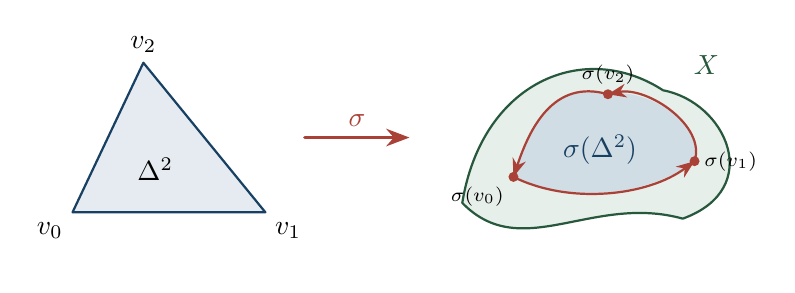
\begin{tikzpicture}[>=Stealth,line cap=round,line join=round]
 \coordinate (a) at (0,0); \coordinate (b) at (2.45,0);
 \coordinate (c) at (.9,1.9);
 \fill[manifoldblue!12] (a)--(b)--(c)--cycle;
 \draw[manifoldblue!70!black,thick] (a)--(b)--(c)--cycle;
 \node[below left] at (a) {$v_0$};
 \node[below right] at (b) {$v_1$};
 \node[above] at (c) {$v_2$};
 \node at (1.05,.55) {$\Delta^2$};
 \draw[->,manifoldred,very thick] (2.95,.95)--(4.28,.95)
  node[midway,above] {$\sigma$};
 \fill[manifoldgreen!12]
  (4.95,.12) .. controls (5.7,-.65) and (6.6,.24) ..
  (7.75,-.08) .. controls (8.8,.3) and (8.3,1.4) ..
  (7.5,1.55) .. controls (6.5,2.2) and (5.2,1.66) ..
  (4.95,.12);
 \draw[manifoldgreen!70!black,thick]
  (4.95,.12) .. controls (5.7,-.65) and (6.6,.24) ..
  (7.75,-.08) .. controls (8.8,.3) and (8.3,1.4) ..
  (7.5,1.55) .. controls (6.5,2.2) and (5.2,1.66) ..
  (4.95,.12);
 \fill[manifoldblue!25,opacity=.7]
  (5.6,.45) .. controls (6.3,.1) and (7.3,.2) .. (7.9,.65)
  .. controls (8.05,1.1) and (7.3,1.6) .. (6.8,1.5)
  .. controls (6.1,1.7) and (5.8,1.05) .. (5.6,.45);
 \draw[manifoldred,thick,->]
  (5.6,.45) .. controls (6.3,.1) and (7.3,.2) .. (7.9,.65);
 \draw[manifoldred,thick,->]
  (7.9,.65) .. controls (8.05,1.1) and (7.3,1.6) .. (6.8,1.5);
 \draw[manifoldred,thick,->]
  (6.8,1.5) .. controls (6.1,1.7) and (5.8,1.05) .. (5.6,.45);
 \foreach \x/\y in {5.6/.45,7.9/.65,6.8/1.5}
  {\fill[manifoldred] (\x,\y) circle(1.8pt);}
 \node[font=\scriptsize,below left] at (5.6,.45) {$\sigma(v_0)$};
 \node[font=\scriptsize,right] at (7.9,.65) {$\sigma(v_1)$};
 \node[font=\scriptsize,above] at (6.8,1.5) {$\sigma(v_2)$};
 \node[manifoldgreen!70!black] at (8.05,1.87) {$X$};
 \node[manifoldblue!70!black] at (6.7,.8) {$\sigma(\Delta^2)$};
\end{tikzpicture}
\caption{Singularny sympleks jest odwzorowaniem do $X$, niekoniecznie
płaskim trójkątem. Jego brzeg liczymy
z ograniczeń odwzorowania $\sigma$ do trzech ścian.}
\label{fig:singular-simplex}
\end{figure}

\begin{stwierdzenie}[Ciągłe odwzorowania działają na homologii]
\label{prop:funktor-singularny}
Jeśli $f:X\to Y$ jest ciągłe, to
$f_\#:C_n(X)\to C_n(Y)$,
$f_\#(\sigma)=f\circ\sigma$,
jest odwzorowaniem łańcuchowym. Wyznacza homomorfizm
$f_*:H_n(X)\to H_n(Y)$, przy czym
$(g\circ f)_*=g_*\circ f_*$ oraz
$(\id_X)_*=\id_{H_n(X)}$.
\end{stwierdzenie}
\begin{proof}
Na pojedynczym generatorze
\[
 \partial(f\circ\sigma)
 =\sum_i(-1)^i f\circ\sigma\circ\iota_i
 =f_\#(\partial\sigma).
\]
Równość na sumach wynika z liniowości.
Zatem obraz cyklu jest cyklem, a obraz
brzegu brzegiem, więc $f_*$ jest
dobrze określony na ilorazie.
Równości dotyczące składania sprawdzamy
już na $\sigma$:
$g_\#f_\#(\sigma)=g\circ f\circ\sigma$.
\end{proof}

\begin{przyklad}[Punkt]
\label{prz:homologia-punktu}
Dla $X=\{*\}$ w każdym stopniu jest
dokładnie jeden singularny sympleks
stały $c_n$, więc $C_n(X)\cong\Z$.
Jego brzeg to
$\partial c_n=(\sum_{i=0}^n(-1)^i)c_{n-1}$:
dla $n$ nieparzystego współczynnik
jest $0$, dla dodatniego parzystego $1$.
Kompleks ma więc postać
\[
 \cdots\xrightarrow{\;0\;}\Z
 \xrightarrow{\;1\;}\Z
 \xrightarrow{\;0\;}\Z
 \xrightarrow{\;1\;}\Z
 \xrightarrow{\;0\;}\Z\longrightarrow0,
\]
gdzie prawy skraj to $C_0$; precyzyjnie
$\partial_1=0$, $\partial_2=1$.
Stąd $H_0(*)=\Z$ i $H_n(*)=0$ dla $n>0$.
\end{przyklad}

\begin{stwierdzenie}[Składowe łukowe]
\label{prop:h0-singularne}
Grupa $H_0(X)$ jest wolna na składowych
łukowych $X$. W szczególności
dla przestrzeni niepustej łukowo spójnej
$H_0(X)\cong\Z$.
\end{stwierdzenie}
\begin{proof}
Każdy punkt $x$ jest singularnym
$0$-sympleksem, więc $C_0(X)$
jest wolną grupą na punktach.
Dla drogi $\gamma:[0,1]=\Delta^1\to X$
mamy $\partial\gamma=[\gamma(1)]-
[\gamma(0)]$. Punkty w jednej składowej
łukowej mają zatem tę samą klasę.
Z drugiej strony każdy składnik
brzegu dowolnego $1$-łańcucha
jest różnicą punktów połączonych drogą:
nie może utożsamić dwóch różnych
składowych. Sumowanie współczynników
punktów osobno w każdej składowej
daje odwrotny homomorfizm do
wolnej grupy na składowych.
\end{proof}

\begin{twierdzenie}[Niezmienniczość homotopijna]
\label{thm:homotopia-singularna}
Jeśli $f,g:X\to Y$ są homotopijne, to
$f_*=g_*:H_n(X)\to H_n(Y)$ w każdym stopniu.
Jeśli $X$ i $Y$ są homotopijnie równoważne,
ich grupy homologii są izomorficzne.
\end{twierdzenie}
\begin{proof}
Niech $F:X\times[0,1]\to Y$ będzie
homotopią, $F(x,0)=f(x)$,
$F(x,1)=g(x)$.
Graniastosłup $\Delta^n\times[0,1]$
dzielimy na $n+1$ zorientowanych
$(n+1)$-sympleksów. Dla $i=0,\ldots,n$
ich uporządkowane wierzchołki to
\[
 (e_0,0),\ldots,(e_i,0),
 (e_i,1),\ldots,(e_n,1).
\]
Niech $T_i:\Delta^{n+1}\to
\Delta^n\times[0,1]$ będzie odwzorowaniem
afinicznym posyłającym kolejne wierzchołki
właśnie na tę listę. Określmy
\[
 P_n(\sigma)=\sum_{i=0}^n(-1)^i\,
 F\circ(\sigma\times\id_{[0,1]})\circ T_i
 \in C_{n+1}(Y).
\]
Rozpiszmy brzeg sumy. Wewnętrzne
$n$-ściany, na których spotykają się
sąsiednie części graniastosłupa,
pojawiają się z przeciwnymi znakami.
Ściany boczne nad każdą ścianą
$\Delta^n$ tworzą dokładnie
$-P_{n-1}(\partial\sigma)$:
jeśli $j<i$, usuwamy dolny wierzchołek $(e_j,0)$
z $T_i$, z łącznym znakiem $(-1)^{i+j}$.
Na pryzmacie ściany naprzeciw $e_j$ punkt podziału ma indeks $i-1$,
więc znak w $-P_{n-1}\partial$ wynosi
$-(-1)^j(-1)^{i-1}=(-1)^{i+j}$.
Jeśli $j>i$, usuwamy górny wierzchołek $(e_j,1)$,
na pozycji $j+1$; oba rachunki dają $(-1)^{i+j+1}$.
Wewnętrzna ściana między $T_{i-1}$ i $T_i$ powstaje
przez usunięcie odpowiednio $(e_{i-1},1)$ i $(e_i,0)$,
ze znakami $-1$ i $+1$.
Pozostałe dwie ściany to górna
$g\circ\sigma$ ze znakiem $+1$
oraz dolna $f\circ\sigma$ ze
znakiem $-1$. Zatem
\begin{equation}\label{eq:prism-identity}
 \partial P_n+P_{n-1}\partial
 =g_\#-f_\#.
\end{equation}
Przyjmujemy $P_{-1}=0$. Dla $n=0$ jest to znana równość
,,koniec drogi minus początek'';
powyższe parowanie ścian dowodzi
jej w każdym wymiarze. W świetle
Twierdzenia~\ref{thm:homotopia-homologia}
oba odwzorowania indukują to samo na homologii.
Jeśli $u:X\to Y$, $v:Y\to X$
są odwrotne z dokładnością do homotopii,
to $(vu)_*=\id$ i $(uv)_*=\id$,
więc $u_*$ i $v_*$ są odwrotne.
\end{proof}

W szczególności przestrzeń ściągalna
ma homologię punktu. Jeśli
$A\subseteq X$ jest retraktem
deformacyjnym, to $H_n(A)\cong H_n(X)$.

\section{Pary przestrzeni i homologia zredukowana}
\label{sec:homologia-wzgledna}

\begin{definicja}[Grupy względne i zredukowane]
\index{grupy wzgledne i zredukowane@Grupy względne i zredukowane}
\label{def:homologia-wzgledna}
Dla $A\subseteq X$ włączenie daje
podkompleks $C_\bullet(A)\subseteq C_\bullet(X)$.
Kładziemy
\[
 C_n(X,A)=C_n(X)/C_n(A),\qquad
 H_n(X,A)=H_n(C_\bullet(X,A)).
\]
\emph{Augmentacja} $\varepsilon:C_0(X)\to\Z$ sumuje
współczynniki punktów. Dołączamy stopień $C_{-1}=\Z$,
z różniczką $\partial_0=\varepsilon$; niższe grupy są zerowe.
Ponieważ $\varepsilon\partial_1=0$, otrzymujemy kompleks,
którego homologie oznaczamy $\widetilde H_n(X)$.
Dla niepustego $X$ mamy
$\widetilde H_0(X)=\ker(\varepsilon:H_0(X)\to\Z)$,
$\widetilde H_n(X)=H_n(X)$ dla $n>0$ i
$\widetilde H_n(X)=0$ dla $n<0$.
Dla $X=\varnothing$ wszystkie grupy łańcuchów w stopniach
nieujemnych są zerowe, więc $\widetilde H_{-1}(\varnothing)=\Z$
i pozostałe grupy zredukowane są zerowe.
\end{definicja}

Względny cykl może mieć brzeg w $A$:
to, co w $X$ jest otwartą powierzchnią,
po ,,pominięciu $A$'' staje się cyklem.
Na przykład zorientowany dysk reprezentuje klasę względną
względem swojego okręgu brzegowego.
Jeżeli $X$ ma skończoną liczbę $c>0$ składowych łukowych,
to $\widetilde H_0(X)\cong\Z^{c-1}$.
Ogólnie, po wyborze jednej składowej $P_0$, bazę jądra
augmentacji tworzą różnice $[P]-[P_0]$ dla $P\ne P_0$:
jest to suma prosta kopii $\Z$, także dla nieskończenie wielu składowych.

\begin{twierdzenie}[Długi ciąg pary]
\label{thm:les-pary}
Każda para $(X,A)$ daje naturalny
długi ciąg dokładny
\begin{equation}\label{eq:les-pary}
 \cdots\to H_n(A)\xrightarrow{i_*}H_n(X)
 \xrightarrow{j_*}H_n(X,A)
 \xrightarrow{\delta}H_{n-1}(A)
 \to H_{n-1}(X)\to\cdots.
\end{equation}
Jeśli $\partial c\in C_{n-1}(A)$,
to $\delta[c]=[\partial c]$.
\end{twierdzenie}
\begin{proof}
W każdej grupie łańcuchów mamy
krótki ciąg dokładny
$0\to C_n(A)\to C_n(X)\to C_n(X,A)\to0$.
Jest zgodny z brzegami, więc
Stwierdzenie~\ref{prop:ses-iloraz}
daje długi ciąg i wzór na $\delta$.
Naturalność pochodzi z przemienności
odwzorowań łańcuchów dla odwzorowań
par $(X,A)\to(Y,B)$.
\end{proof}

Jeśli $A\ne\varnothing$, możemy w tym ciągu zastąpić homologie
$A$ i $X$ zredukowanymi, pozostawiając zwykłą homologię względną.
Istotnie, w stopniu $-1$ włączenie kompleksów augmentowanych
jest identycznością $\Z\to\Z$, więc ich iloraz ma tam zero
i jest właśnie kompleksem $C_\bullet(X,A)$.

Homotopia par (w każdym czasie obraz $A$
leży w $B$) daje te same odwzorowania na $H_n(X,A)$:
pryzmat z dowodu Twierdzenia~\ref{thm:homotopia-singularna}
przenosi $C_\bullet(A)$ do $C_{\bullet+1}(B)$,
więc wzór~\eqref{eq:prism-identity}
schodzi na kompleksy ilorazowe.

\section{Podział barycentryczny, wycinanie i sklejanie}
\label{sec:wycinanie-homologia}

Homologia singularna ma nieskończenie wiele generatorów nawet
dla prostych przestrzeni. Podział dużego sympleksu na małe
części pozwala jednak sprowadzić rachunek do lokalnych
fragmentów. Z tego mechanizmu wynika wycinanie.

\begin{lemat}[Małe łańcuchy]
\label{lem:male-lancuchy}
Niech $\mathcal U=\{U_\alpha\}$ będzie otwartym
pokryciem $X$. Podkompleks
$C_n^{\mathcal U}(X)\subseteq C_n(X)$
generowany przez sympleksy, których obrazy
leżą w jednym $U_\alpha$, ma te same
grupy homologii co $C_\bullet(X)$.
Włączenie indukuje izomorfizmy w każdym stopniu.
\end{lemat}
\begin{proof}
Podamy konstrukcję potrzebną w obu kierunkach.
Podzielmy liniowo $\Delta^n$ na sympleksy
barycentryczne: wierzchołkami małego sympleksu
są barycentra łańcucha niepustych ścian
$F_0\subsetneq F_1\subsetneq\cdots\subsetneq F_n$,
zapisane w tej właśnie kolejności. Każdy taki łańcuch odpowiada
permutacji $\pi$ wierzchołków: $F_j=[e_{\pi(0)},\ldots,e_{\pi(j)}]$.
Niech $a_\pi:\Delta^n\to\Delta^n$ będzie afinicznym odwzorowaniem
na uporządkowany mały sympleks. Określamy
\[
 S_n(\sigma)=\sum_{\pi\in S_{n+1}}\operatorname{sgn}(\pi)
                 \,\sigma\circ a_\pi.
\]
Znak pochodzi z orientacji: dla permutacji identycznościowej
macierz kolejnych barycentrów ma dodatni wyznacznik w otoczce afinicznej,
a permutacja wierzchołków zmienia go o $\operatorname{sgn}(\pi)$.
Kolejność barycentrów jest ważna: w kompleksie singularnym
odwrócenie parametryzacji nie jest z definicji ujemnym generatorem.
Ściany wewnętrzne dwóch części
występują z przeciwnymi znakami,
a ich ściany na zewnątrz dają
podział odpowiedniej ściany $\sigma$.
Dokładniej, wewnętrzną ścianę uzyskujemy, pomijając barycentrum $F_j$
dla $j<n$. Dwie odpowiadające jej permutacje zamieniają miejscami
pozycje $j,j+1$, więc mają przeciwne znaki, a pozostałe
uporządkowane barycentra są identyczne. Dla $j=n$ otrzymujemy
sympleks podziału ściany naprzeciw $e_{\pi(n)}$.
Jeśli $\rho$ jest permutacją pozostałych wierzchołków w ich
odziedziczonej kolejności, to
$(-1)^n\operatorname{sgn}(\pi)=(-1)^{\pi(n)}\operatorname{sgn}(\rho)$.
To właśnie znak tej ściany w $S\partial$; stąd $\partial S=S\partial$.

Wyjaśnijmy też, dlaczego $S$ nie zmienia
klasy homologii. Na standardowym sympleksie
oznaczmy jego identycznościowe odwzorowanie
przez $u_n$ i indukcyjnie zbudujmy
łańcuchy $t_n$ tak, aby dla $n\geq1$
\[
 \partial t_n+\sum_{i=0}^n(-1)^i(\iota_i)_\#t_{n-1}
       =S(u_n)-u_n. \tag{*}
\]
W stopniu $0$ obie strony są zerowe,
więc $t_0=0$. Jeśli mamy już konstrukcję
na wszystkich ścianach, to oznaczmy ich sumę
$b_n=\sum_i(-1)^i(\iota_i)_\#t_{n-1}$.
Łańcuch $z=S(u_n)-u_n-b_n$
jest cyklem: stosując $\partial$,
używamy $\partial S=S\partial$,
równości (*) na ścianach
i $\partial^2=0$.
W wypukłym $\Delta^n$ taki cykl jest
brzegiem: z barycentrum $b$ łączymy
każdy jego singularny sympleks prostym
stożkiem. Dla $\tau:\Delta^k\to\Delta^n$ stożek $b*\tau$
ma wzór
\[
 (b*\tau)(s_0,\ldots,s_{k+1})
 =s_0b+(1-s_0)\tau\left(\frac{s_1}{1-s_0},\ldots,
                         \frac{s_{k+1}}{1-s_0}\right)
 \quad(s_0<1),
\]
z wartością $b$ dla $s_0=1$. Jest ciągły także w tym wierzchołku,
bo obraz $\tau$ jest ograniczony. Brzeg tego stożka to
$\tau-b*(\partial\tau)$ (dla $0$-sympleksu
dodatkowo odejmujemy punkt $b$);
po zsumowaniu nad cyklem składniki
stożkowe się kasują. Daje to $t_n$.
Przenosząc $t_n$ przez dowolne
$\sigma:\Delta^n\to X$, otrzymujemy
operator $T_n(\sigma)=\sigma_\#t_n$ o nośniku zawartym
w $\sigma(\Delta^n)$, który spełnia
\[
 \partial T+T\partial=S-\id.
\]
Zatem $S^r-\id=\partial T^{(r)}+
T^{(r)}\partial$, gdzie
$T^{(r)}=T+ST+\cdots+S^{r-1}T$.

Średnice części po kolejnych podziałach
barycentrycznych dążą do zera: dla
$n$-sympleksu każdy nowy wierzchołek
jest średnią wierzchołków pewnej ściany,
a nowa krawędź łączy barycentra zagnieżdżonych ścian.
Jeśli mają one $p<q\leq n+1$ wierzchołków, to
$b_G=(p/q)b_F+((q-p)/q)b_{G\setminus F}$.
Zatem $\|b_G-b_F\|\leq(q-p)\operatorname{diam}(\Delta)/q
\leq n\operatorname{diam}(\Delta)/(n+1)$.
Średnica wypukłego sympleksu jest największą odległością jego
wierzchołków, więc dla $n\geq1$ otrzymujemy geometryczny spadek
średnic (także na ścianach). Dla $n=0$ sympleks jest już punktem. Dla danego $\sigma$
przeciwobrazy $U_\alpha$ tworzą
otwarte pokrycie zwartego $\Delta^n$;
jego liczba Lebesgue'a jest dodatnia.
Po dostatecznie wielu podziałach
każda część trafia przez $\sigma$
do jednego $U_\alpha$.
Każdy łańcuch jest skończoną sumą,
więc można wybrać wspólne $r$
dla wszystkich jego sympleksów.

Jeśli $z$ jest cyklem, $S^rz$
jest mały i różni się od $z$
o $\partial T^{(r)}z$; to dowodzi
surjektywności na homologii.
Jeśli mały cykl $z$ jest brzegiem
$c$ w pełnym kompleksie, podzielmy
$c$ tak wiele razy, by $S^rc$
był mały. Łańcuch $T^{(r)}z$
też jest mały, ponieważ każda
jego część leży w obrazie
jednego pierwotnego, małego sympleksu.
Równości $\partial c=z$ i
$\partial T^{(r)}z=S^rz-z$ dają
\[
 \partial\bigl(S^rc-T^{(r)}z\bigr)=z.
\]
Zatem $z$ jest brzegiem już
w podkompleksie małych łańcuchów:
otrzymujemy iniektywność.
\end{proof}

Stożkowanie wypełnia każdy cykl dodatniego stopnia w wypukłym
sympleksie, a w stopniu zero tylko cykl o sumie współczynników zero.
W konstrukcji $T$ stopień zero załatwiamy przez $t_0=0$,
bo $S_0=\id$. Lokalność $T$ jest istotna dla dowodu iniektywności.

\begin{twierdzenie}[Wycinanie]
\label{thm:wycinanie}
Jeżeli $Z\subseteq A\subseteq X$ oraz
$\overline Z\subseteq\operatorname{int}_X A$,
to włączenie par
\[
 (X\setminus Z,A\setminus Z)\longrightarrow(X,A)
\]
indukuje izomorfizm na wszystkich
grupach homologii względnej.
\end{twierdzenie}
\begin{proof}
Oznaczmy $U=X\setminus\overline Z$
oraz $V=\operatorname{int}_X A$.
To otwarte pokrycie $X$;
po ograniczeniu do $X\setminus Z$
otrzymujemy pokrycie
$\{U,V\setminus Z\}$.
Lemat~\ref{lem:male-lancuchy} działa
także po wzięciu ilorazu przez
łańcuchy w $A$: izomorfizmy
dla $A$ i $X$, zestawione
z długimi ciągami par, dają
izomorfizm dla odpowiadających
kompleksów względnych
(Lemat~\ref{lem:pieciu}).

Policzmy teraz te małe kompleksy.
Ponieważ $V\subseteq A$,
\[
 C_\bullet^{\{U,V\}}(X)
   =C_\bullet(U)+C_\bullet(V),\qquad
 C_\bullet^{\{U,V\}}(A)
   =C_\bullet(U\cap A)+C_\bullet(V).
\]
Ich iloraz jest kanonicznie
$C_\bullet(U)/C_\bullet(U\cap A)$:
sympleks należący jednocześnie do
$U$ i $V$ należy do $U\cap A$,
więc jądro tej identyfikacji jest
dokładnie wskazanym podkompleksem.
Analogiczny iloraz dla
$(X\setminus Z,A\setminus Z)$
i jego pokrycia jest \emph{tym samym}
kompleksem
$C_\bullet(U)/C_\bullet(U\cap A)$.
Włączenie par staje się na tych
modelach identycznością, co
kończy dowód.
\end{proof}

Wycinanie mówi, że usunięcie części
leżącej głęboko we wnętrzu $A$
nie zmienia tego, co para $(X,A)$
mierzy \emph{poza} $A$. Warunek
o domknięciu ma znaczenie:
zapewnia otwarte pokrycia użyte
w dowodzie.

\begin{twierdzenie}[Ciąg Mayera--Vietorisa]
\label{thm:mv-przestrzenie}
Jeśli $X=U\cup V$, gdzie $U,V$
są otwarte w $X$, to istnieje
długi ciąg dokładny
\begin{equation}\label{eq:mv-przestrzenie}
 \cdots\to H_n(U\cap V)
 \xrightarrow{(i_*,-j_*)}
 H_n(U)\oplus H_n(V)
 \xrightarrow{k_*+\ell_*}H_n(X)
 \xrightarrow{\delta}H_{n-1}(U\cap V)\to\cdots.
\end{equation}
Tak samo działają grupy zredukowane.
\end{twierdzenie}
\begin{proof}
Wewnątrz $C_\bullet(X)$ rozważmy
$B_\bullet=C_\bullet(U)+C_\bullet(V)$.
Mamy krótki ciąg kompleksów
\[
 0\to C_\bullet(U\cap V)
 \xrightarrow{c\mapsto(c,-c)}
 C_\bullet(U)\oplus C_\bullet(V)
 \xrightarrow{(a,b)\mapsto a+b}
 B_\bullet\to0.
\]
Iniektywność pierwszego odwzorowania jest jasna;
jądro drugiej składa się z par
$(c,-c)$, w których każdy singularny
sympleks występujący w $c$ należy
zarazem do $U$ i do $V$.
Surjektywność wynika z definicji sumy.
Ponadto $B_\bullet=C_\bullet^{\{U,V\}}(X)$,
więc Lemat~\ref{lem:male-lancuchy}
identyfikuje $H_*(B)$ z $H_*(X)$.
Zastosowanie Twierdzenia~\ref{thm:les-homologia}
daje~\eqref{eq:mv-przestrzenie}.
W wersji zredukowanej dołączamy
do każdego kompleksu stopień $-1$
równy $\Z$ i różniczkę
$\varepsilon:C_0\to\Z$.
Na stopniu $-1$ ten sam krótki
ciąg ma postać
$0\to\Z\xrightarrow{c\mapsto(c,-c)}
\Z\oplus\Z\xrightarrow{(a,b)\mapsto a+b}
\Z\to0$, nadal dokładną.
W stopniach nieujemnych
obowiązuje poprzedni rachunek.
Homologie tych powiększonych
kompleksów są właśnie
homologiami zredukowanymi;
dotyczy to również pustego
przecięcia, dla którego
$\widetilde H_{-1}(\varnothing)=\Z$.
\end{proof}

Jeśli $c=a+b\in B_n$ jest cyklem,
gdzie $a\in C_n(U)$ i $b\in C_n(V)$,
to $\partial a=-\partial b$ jest
łańcuchem w $U\cap V$, a
$\delta[c]=[\partial a]$ z wyborem
znaku zgodnym z pierwszym odwzorowaniem.
To praktyczna recepta na odwzorowanie łączące.

\begin{przyklad}[Okrąg z dwóch łuków]
\label{prz:mv-okrag}
Pokryjmy $S^1$ dwoma otwartymi,
ściągalnymi łukami $U,V$, których
przecięcie składa się z dwóch
łuków. Mamy
$\widetilde H_0(U)=
\widetilde H_0(V)=0$,
a $\widetilde H_0(U\cap V)\cong\Z$
generuje różnica klas punktów
z dwóch składowych.
Zredukowany ciąg
Mayera--Vietorisa daje
\[
 0=\widetilde H_1(U)\oplus
 \widetilde H_1(V)\to
 \widetilde H_1(S^1)
 \xrightarrow[\cong]{\delta}
 \widetilde H_0(U\cap V)\to0.
\]
Zatem $H_1(S^1)\cong\Z$.
Geometria odwzorowania $\delta$ jest prosta:
rozcinając cykl okręgu na łuki
leżące w $U$ i $V$, otrzymujemy
dwa końce w różnych składowych
ich przecięcia.
\end{przyklad}

\begin{twierdzenie}[Homologia sfer]
\label{thm:homologia-sfer}
Dla $n\geq0$:
\[
 \widetilde H_k(S^n;\Z)=
 \begin{cases}\Z,&k=n,\\0,&k\ne n.\end{cases}
\]
Ponadto dla $n\geq1$
\[
 H_k(D^n,S^{n-1};\Z)=
 \begin{cases}\Z,&k=n,\\0,&k\ne n.\end{cases}
\]
\end{twierdzenie}
\begin{proof}
$S^0$ ma dwie składowe punktowe:
$H_0(S^0)=\Z^2$ oraz
$\widetilde H_0(S^0)=\Z$.
Wyższa homologia znika, bo jest
to suma dwóch kopii homologii
punktu z Przykładu~\ref{prz:homologia-punktu}.

Dla $n\geq1$ weźmy lekko
powiększone otwarte półkule
$U,V\subset S^n$. Każda jest
ściągalna, a $U\cap V$
deformacyjnie zwija się na
sferę równikową $S^{n-1}$.
Zredukowany ciąg
Mayera--Vietorisa, wraz z
zerowaniem homologii $U,V$,
daje dla każdego $k$ izomorfizm
\[
 \widetilde H_k(S^n)
 \xrightarrow{\ \cong\ }
 \widetilde H_{k-1}(S^{n-1}).
\]
W stopniu $k=1$ używa się
właśnie zredukowanego $H_0$;
gdy $n=1$, obie składowe
przecięcia są niezbędne.
Indukcja od $S^0$ daje pierwszy wzór.

Dysk $D^n$ jest ściągalny. W ciągu
zredukowanym pary $(D^n,S^{n-1})$
grupy dysku są zerowe, a odwzorowanie
łączące daje
$H_k(D^n,S^{n-1})\cong
\widetilde H_{k-1}(S^{n-1})$
dla $k\geq1$. Dla $k=0$
odwzorowanie $H_0(S^{n-1})\to H_0(D^n)$
jest surjekcją, więc grupa
względna również znika.
To daje drugi wzór.
\end{proof}

\begin{uwaga}[Klasa fundamentalna i orientacja]
Generator $H_n(D^n,S^{n-1})\cong\Z$
nazywamy \emph{klasą orientacji dysku}.
Wybór jednego z jego dwóch znaków
określa orientację; w długim ciągu
pary $\delta$ posyła ją na
generator $\widetilde H_{n-1}(S^{n-1})$.
Różniczkowe ujęcie orientacji
i całkowania pozostawiamy
osobnemu rozdziałowi.
\end{uwaga}

\section{Od triangulacji do homologii przestrzeni}
\label{sec:porownanie-symplicjalne}

Dla kompleksu symplicjalnego zachowujemy ustalony porządek
wierzchołków, a dla $\Delta$-kompleksu porządki jego map charakterystycznych.
Każdy bazowy sympleks $\sigma:\Delta^n\to|K|$ jest wtedy
jednocześnie singularnym sympleksem. Daje to odwzorowanie łańcuchowe
\[
 I:C_\bullet^\Delta(K)\longrightarrow C_\bullet(|K|),
 \qquad [\sigma]\longmapsto \sigma,
\]
bo oba operatory $\partial$ sumują te same
ściany z tymi samymi znakami.
Mapę $I$ rozszerzamy liniowo: na przykład $I(-[\sigma])=-\sigma$.
Nie zastępujemy prawej strony osobnym generatorem otrzymanym
przez odwrócenie parametryzacji. Nie jest to
izomorfizm grup łańcuchów: po prawej są
wszystkie odwzorowania ciągłe, po lewej tylko
wybrane sympleksy. Niezwykłe jest to,
że po przejściu do homologii różnica znika.

Potrzebny będzie prosty sposób traktowania
komórki z całym brzegiem zwiniętym do punktu.

\begin{lemat}[Iloraz pary komórkowej]
\label{lem:iloraz-cw-homologia}
Niech $A\ne\varnothing$ będzie podkompleksem skończonego
kompleksu CW $X$. Jeśli istnieje otwarte
otoczenie $N$ zbioru $A$, które silnie
deformacyjnie retrahuje się na $A$, to
odwzorowanie ilorazowe indukuje izomorfizm
\[
 H_k(X,A)\xrightarrow{\ \cong\ }
 H_k(X/A,\{*\})=\widetilde H_k(X/A)
 \quad(k\geq0).
\]
Takie otoczenie istnieje, gdy
$A=X^{n-1}\ne\varnothing$ i $X=X^n$ jest skończonym
szkieletem CW dla $n\geq1$, a także gdy do skończonego $A$
dołączamy pojedynczą komórkę dodatniego wymiaru.
\end{lemat}
\begin{proof}
Włączenie $A\hookrightarrow N$ jest
równoważnością homotopijną. Porównując
długie ciągi par $(X,A)$ i $(X,N)$
za pomocą Lematu~\ref{lem:pieciu},
dostajemy $H_k(X,A)\cong H_k(X,N)$.
Po zwinięciu $A$ do punktu homotopia schodzi na $N/A$.
Uzasadnijmy jej ciągłość również względem czasu.
Skończony kompleks CW jest zwarty, bo jest obrazem skończonej
sumy zwartych dysków; domknięty $A$ też jest zwarty.
Projekcja $q:N\to N/A$ jest domknięta: dla domkniętego $F\subseteq N$
zbiór $q^{-1}q(F)$ jest równy $F$ lub $F\cup A$.
Ma zwarte włókna, więc $q\times\id_I$ jest również domknięta.
Istotnie, jeśli domknięty zbiór omija włókno nad $(y,t)$,
skończone pokrycie tego włókna prostokątami otwartymi daje
otoczenia $O\supseteq q^{-1}(y)$ i $J\ni t$ z $O\times J$
rozłącznym z tym zbiorem; domkniętość $q$ daje otoczenie
$W\ni y$ takie, że $q^{-1}(W)\subseteq O$.
Stąd $(q\times\id_I)$ jest odwzorowaniem ilorazowym,
co pozwala przenieść homotopię. Zatem $N/A$ silnie zwija się do $\{*\}$,
więc tak samo
$H_k(X/A,\{*\})\cong H_k(X/A,N/A)$.

Porównajmy środkowe grupy.
Zbiór $A$ jest domknięty
(dla skończonego CW wynika to
z topologii słabej), zatem
$\{X\setminus A,N\}$ jest
otwartym pokryciem $X$.
W ilorazie mamy pokrycie
$\{(X/A)\setminus\{*\},N/A\}$.
Lemat o małych łańcuchach,
zastosowany również do $N$,
pozwala obliczać homologie
tych dwóch par odpowiednio za pomocą kompleksów
\[
 \frac{C_\bullet(X\setminus A)}
      {C_\bullet(N\setminus A)}
 \quad\text{oraz}\quad
 \frac{C_\bullet((X/A)\setminus\{*\})}
      {C_\bullet((N/A)\setminus\{*\})}.
\]
Poza $A$ odwzorowanie ilorazowe jest
homeomorfizmem, więc te dwa
kompleksy są izomorficzne.
Składając trzy izomorfizmy,
otrzymujemy tezę.

Dla $A=X^{n-1}\subset X^n$
weźmy $N$ złożony z $A$ oraz,
w każdej dołączonej $n$-komórce,
obrazu pierścienia
$\{x\in D^n:\|x\|>1/2\}$.
Jest otwarty w topologii
nadanej przez odwzorowania dołączające.
W każdym pierścieniu promieniowo
przesuwamy $r$ od wartości
$r>1/2$ do $1$, pozostawiając
brzeg i cały $A$ nieruchome.
Na częściach dyskowych używamy wzoru
$ru\mapsto((1-t)r+t)u$. Ciągłość przy $A$ sprawdzamy jak
w dowodzie Twierdzenia~\ref{thm:pi1-dolaczenie-komorki}:
w każdym otoczeniu zachowujemy tylko te punkty pasa, których
cały odcinek radialny do brzegu mieści się w tym otoczeniu.
Te mniejsze zbiory są otwarte i pozostają w pierwotnym otoczeniu
przez cały czas homotopii. Daje to silną retrakcję $N\to A$.
Ten sam argument działa przy dołączeniu pojedynczej komórki.
\end{proof}

\begin{lemat}[Generator pojedynczego sympleksu]
\label{lem:orientacja-simpleksu}
Identycznościowe odwzorowanie singularne
$u_n:\Delta^n\to\Delta^n$ określa
generator
$H_n(\Delta^n,\partial\Delta^n)\cong\Z$
dla $n\geq1$.
\end{lemat}
\begin{proof}
Jest cyklem względnym, bo jego
brzeg leży w $\partial\Delta^n$.
Brzeg sympleksu jest sferą
(Stwierdzenie~\ref{prop:brzeg-sympleksu}),
a jej homologię policzyliśmy
w Twierdzeniu~\ref{thm:homologia-sfer}.
Wynika stąd, że odwzorowanie łączące
\[
 \delta:H_n(\Delta^n,\partial\Delta^n)
 \longrightarrow
 \widetilde H_{n-1}(\partial\Delta^n)
 \]
jest izomorfizmem i posyła
$[u_n]$ na klasę cyklu
$\partial u_n$.
Pokażemy indukcyjnie, że ten
cykl jest generatorem.
Dla $n=1$ jest to różnica
końców, generator
$\widetilde H_0(S^0)$.
W wyższym wymiarze rozdzielmy
$\partial\Delta^n$ na jedną
ścianę $F\cong\Delta^{n-1}$
i sumę $B$ pozostałych ścian.
$F$ i $B$ są ściągalne:
$B$ jest stożkiem z przeciwległego
wierzchołka nad $\partial F$;
ich przecięciem jest $\partial F$.
W ciągu Mayera--Vietorisa
odwzorowanie łączące
$\widetilde H_{n-1}(\partial\Delta^n)
\to\widetilde H_{n-2}(\partial F)$
jest izomorfizmem. Aby zastosować wersję dla zbiorów otwartych, przedstawmy
oba dyski $F,B$ jako stożki nad ich wspólnym brzegiem $\partial F$.
Niech $r\in[0,1]$ oznacza w każdym z nich parametr radialny,
z $r=1$ na $\partial F$. Zbiory
$U=F\cup\{x\in B:r(x)>1/2\}$ oraz
$V=B\cup\{x\in F:r(x)>1/2\}$ są otwarte w $F\cup B$:
na każdej z dwóch części ich przeciwobrazy są otwarte.
Przesuwając dodatkowe pasy do $r=1$, retrahujemy je na $F,B$,
a ich przecięcie na $\partial F$.
Cykl $\partial u_n$ jest sumą
$\pm u_F$ na $F$ i pozostałych
ścian na $B$; jego obrazem przez
odwzorowanie łączące jest
$\pm[\partial u_F]$.
To generator na mocy
założenia indukcyjnego.
Zatem $\partial u_n$, a więc
również $u_n$ względnie,
jest generatorem.
\end{proof}

\begin{twierdzenie}[Porównanie homologii]
\label{thm:symplicjalna-singularna}
Dla skończonego kompleksu symplicjalnego
$K$ naturalne odwzorowanie indukuje
\[
 I_*:H_n^\Delta(K)\xrightarrow{\ \cong\ }
 H_n(|K|;\Z)
 \qquad(n\geq0).
\]
To samo zachodzi dla skończonego
$\Delta$-kompleksu, jeśli generatory
po lewej to jego sympleksy
charakterystyczne z ich ścianami.
\end{twierdzenie}
\begin{proof}
Uporządkujmy sympleksy tak, aby
każdy pojawiał się po wszystkich
swoich ścianach. Budujemy kompleks
po jednym sympleksie:
$L\subset K=L\cup_\varphi\Delta^n$.
Załóżmy indukcyjnie, że porównanie
jest izomorfizmem dla $L$.
Iloraz kompleksów symplicjalnych
$C^\Delta(K)/C^\Delta(L)$
ma jeden generator w stopniu $n$
i zero w pozostałych stopniach,
więc jego homologia jest $\Z$
tylko w stopniu $n$.

Jeśli $n\geq1$, po zwinięciu $L$
do punktu przestrzeń $|K|/|L|$
jest $\Delta^n/\partial\Delta^n
\cong S^n$; analogiczny opis
działa dla $\Delta$-kompleksu,
nawet gdy jego ściany były
między sobą utożsamione.
Lemat~\ref{lem:iloraz-cw-homologia}
i Twierdzenie~\ref{thm:homologia-sfer}
dają $H_q(|K|,|L|)=\Z$ dla
$q=n$ i zero w innych stopniach.
Odwzorowanie względne przenosi jedyny
generator na klasę charakterystycznego sympleksu.
Mapa par $(\Delta^n,\partial\Delta^n)\to(|K|,|L|)$
indukuje homeomorfizm ich ilorazów: jest ciągłą bijekcją
ze zwartej przestrzeni do przestrzeni Hausdorffa.
Naturalność map do ilorazów w Lemacie~\ref{lem:iloraz-cw-homologia}
pokazuje, że także na homologii względnej jest izomorfizmem.
Na mocy Lematu~\ref{lem:orientacja-simpleksu} przenosi więc
generator na generator, a nie na jego dowolną wielokrotność.
Dla $n=0$ nowy wierzchołek jest
osobną składową i odpowiednie
odwzorowanie względne jest izomorfizmem
$\Z\to\Z$ w stopniu $0$.

Mamy teraz przemienny diagram
długich ciągów par dla kompleksów
symplicjalnych i singularnych.
Na wyrazach dotyczących $L$
odwzorowania pionowe są izomorfizmami
z założenia indukcyjnego,
a na względnych właśnie
to pokazaliśmy. Lemat~\ref{lem:pieciu}
zastosowany do kolejnych pięciu
wyrazów daje izomorfizm dla $K$.
Zaczynamy od kompleksu pustego,
dla którego wszystkie zwykłe
grupy homologii są zerowe.
\end{proof}

W praktyce wolno zatem obliczać
homologię przestrzeni z jednej
wygodnej triangulacji: otrzymany
wynik nie zależy od wyboru
triangulacji. Podziały sympleksów
zmieniają grupy łańcuchów,
ale nie grupy homologii.

\section{Homologia komórkowa}
\label{sec:homologia-komorkowa}

W triangulacji torusa potrzeba
trójkątów i ich ścian. Struktura
CW z Sekcji~\ref{sec:cw-kompleksy}
może opisywać go jednym punktem,
dwoma pętlami i jedną
$2$-komórką. Homologia komórkowa
zachowuje tę oszczędność.

\begin{twierdzenie}[Względna homologia warstwy komórek]
\label{thm:warstwa-komorek}
Niech $X$ będzie skończonym
kompleksem CW, $X^n$ jego
$n$-szkieletem i $X^{-1}=\varnothing$.
Dla $n\geq1$:
\[
 H_k(X^n,X^{n-1})
 \cong
 \begin{cases}
 \displaystyle\bigoplus_{\alpha\in I_n}\Z[e_\alpha^n],
 &k=n,\\[3pt]0,&k\ne n,
 \end{cases}
\]
gdzie $I_n$ oznacza zbiór $n$-komórek.
Dla $n=0$ mamy
$H_0(X^0)=\bigoplus_{\alpha\in I_0}\Z[e_\alpha^0]$
i $H_k(X^0)=0$ dla $k\ne0$.
\end{twierdzenie}
\begin{proof}
Jeśli $X^{n-1}=\varnothing$ i $n\geq1$, to również $X^n=\varnothing$:
nie można dołączyć dysku o niepustym brzegu do pustej przestrzeni.
Teza jest wtedy oczywista. W pozostałych przypadkach
w ilorazie $X^n/X^{n-1}$
brzeg każdej dołączonej kopii
$D^n$ staje się jednym punktem,
a wnętrza komórek pozostają
rozłączne. Z definicji topologii
CW otrzymujemy bukiet
$\bigvee_{\alpha\in I_n}
(D^n/\partial D^n)\cong
\bigvee_{\alpha\in I_n}S^n$.
Lemat~\ref{lem:iloraz-cw-homologia}
zamienia homologię względną
na zredukowaną homologię bukietu.
Dla skończonego bukietu
zredukowana homologia jest sumą
zredukowanych homologii składników:
dołączamy kolejne sfery. Dla bukietu $Y\vee S^n$
bierzemy $U=Y\cup B$ i $V=S^n\cup N$, gdzie $B$ jest małą
otwartą kulą wokół punktu wspólnego w nowej sferze, a $N$
jest sumą takich kul w dotychczasowych sferach.
Te zbiory są otwarte w topologii ilorazowej bukietu,
retrahują się na $Y,S^n$, a $U\cap V=N\vee B$ jest ściągalne.
Ciąg Mayera--Vietorisa daje izomorfizm indukowany włączeniami
składników, a więc właśnie ich sumę prostą.
Twierdzenie~\ref{thm:homologia-sfer}
daje wskazane grupy.
Znaki generatorów zależą
od wyboru orientacji komórek.
Dla $n=0$ mamy skończony
zbiór punktów; rachunek wynika
z homologii punktu.
\end{proof}

\begin{definicja}[Kompleks komórkowy]
\index{kompleks komorkowy@Kompleks komórkowy}
\label{def:kompleks-komorkowy}
Kładziemy
$C_n^{\mathrm{CW}}(X)=H_n(X^n,X^{n-1})$.
Dla $n\geq1$ jego operator brzegu
jest złożeniem
\begin{equation}\label{eq:cellular-boundary}
 H_n(X^n,X^{n-1})
 \xrightarrow{\ \delta_n\ }
 H_{n-1}(X^{n-1})
 \xrightarrow{\ j_{n-1}\ }
 H_{n-1}(X^{n-1},X^{n-2}),
\end{equation}
gdzie $\delta_n$ pochodzi z
długiego ciągu pary, a
$j_{n-1}$ z ilorazu łańcuchów.
Przyjmujemy $\partial_0^{\mathrm{CW}}=0$.
\end{definicja}

\begin{twierdzenie}[Komórki obliczają homologię]
\label{thm:komorkowa-singularna}
Operator~\eqref{eq:cellular-boundary}
spełnia $(\partial^{\mathrm{CW}})^2=0$.
Dla skończonego CW istnieją
izomorfizmy
\[
 H_n(C_\bullet^{\mathrm{CW}}(X),
       \partial^{\mathrm{CW}})
 \cong H_n(X;\Z)
 \qquad\text{dla każdego }n\geq0.
\]
\end{twierdzenie}
\begin{proof}
Dla $n=1$ równość brzegu brzegu wynika z $\partial_0^{\mathrm{CW}}=0$.
Dla $n\geq2$ z dokładności długiego ciągu
pary $(X^{n-1},X^{n-2})$
wynika $\delta_{n-1}j_{n-1}=0$.
Stąd
\[
 \partial^{\mathrm{CW}}_{n-1}
 \partial^{\mathrm{CW}}_n
 =j_{n-2}\delta_{n-1}j_{n-1}\delta_n=0.
\]

Rozpiszmy porównanie homologii.
Indukcja po szkieletach,
z użyciem długiego ciągu pary
i Twierdzenia~\ref{thm:warstwa-komorek},
daje $H_k(X^m)=0$ dla $k>m$.
Włączenie $X^{m-1}\hookrightarrow X^m$
indukuje ponadto izomorfizm na
$H_k$ dla $k<m-1$: dwa sąsiednie
wyrazy względne o stopniach
$k+1$ i $k$ są wtedy zerowe.
W szczególności komórki wymiaru
$\geq n+2$ nie zmieniają $H_n$.

Dla $n\geq1$ w ciągu pary
$(X^n,X^{n-1})$ mamy odcinek
\[
 0=H_n(X^{n-1})\longrightarrow
 H_n(X^n)\xrightarrow{\ j_n\ }
 C_n^{\mathrm{CW}}
 \xrightarrow{\ \delta_n\ }
 H_{n-1}(X^{n-1}).
\]
Odwzorowanie $j_{n-1}:H_{n-1}(X^{n-1})
\to C_{n-1}^{\mathrm{CW}}$
jest iniektywne: jego jądro
jest obrazem
$H_{n-1}(X^{n-2})=0$.
Dla $n=1$ używamy
$X^{-1}=\varnothing$, co daje
ten sam wniosek.
Zatem $\ker\partial_n^{\mathrm{CW}}
=\ker\delta_n=\operatorname{im}j_n$
i $j_n$ identyfikuje cykle
komórkowe z $H_n(X^n)$.

W następnym długim ciągu,
dla $(X^{n+1},X^n)$,
\[
 C_{n+1}^{\mathrm{CW}}
 \xrightarrow{\ \delta_{n+1}\ }
 H_n(X^n)\longrightarrow
 H_n(X^{n+1})\longrightarrow
 H_n(X^{n+1},X^n)=0.
\]
Jądro przejścia do $H_n(X^{n+1})$
jest więc $\operatorname{im}\delta_{n+1}$.
Po włożeniu w $C_n^{\mathrm{CW}}$
przez $j_n$ jest to dokładnie
$\operatorname{im}\partial_{n+1}^{\mathrm{CW}}$.
Otrzymujemy
$H_n^{\mathrm{CW}}(X)\cong
H_n(X^{n+1})\cong H_n(X)$.
Dla $n=0$ ten sam argument działa
z $H_0(X^0)=C_0^{\mathrm{CW}}$:
$H_0(X^1)$ jest ilorazem przez
obrazy brzegów $1$-komórek,
a wyższe komórki już nie
zmieniają $H_0$.
\end{proof}

\section{Odwzorowania dołączające i konkretne obliczenia}
\label{sec:obliczenia-homologii}

\begin{definicja}[Stopień odwzorowania sfer]
\index{stopien odwzorowania sfer@Stopień odwzorowania sfer}
\label{def:stopien-sfer}
Dla $m\geq1$ każde ciągłe odwzorowanie
$h:S^m\to S^m$ indukuje
endomorfizm $H_m(S^m)\cong\Z$.
Istnieje więc dokładnie jedna
liczba całkowita $\deg h$ taka,
że $h_*([S^m])=(\deg h)[S^m]$.
Nazywamy ją \emph{stopniem} $h$.
\end{definicja}

Z definicji i funktorialności
$\deg(\id)=1$ oraz
$\deg(h\circ g)=\deg h\deg g$.
Homotopijne odwzorowania mają ten sam
stopień. Na $S^1=\{z\in\C:|z|=1\}$
odwzorowanie $z\mapsto z^r$ ma stopień $r\in\Z$.
Uzasadnijmy przejście od liczby obiegów do homologii.
Pętla $\gamma(t)=e^{2\pi it}$ reprezentuje generator $H_1(S^1)$:
po podziale na łuki jej obraz przez izomorfizm Mayera--Vietorisa
z Przykładu~\ref{prz:mv-okrag} jest różnicą punktów dwóch składowych przecięcia.
Dla dowolnych dwóch pętli $\alpha,\beta$ opartych w tym samym punkcie
mamy $[\alpha*\beta]=[\alpha]+[\beta]$ w $H_1$.
Istotnie, złożenie $\alpha*\beta$ z afinicznym odwzorowaniem
$\Delta^2\to[0,1]$ o wartościach $0,1/2,1$ w kolejnych wierzchołkach
jest singularnym $2$-sympleksem o brzegu
$\beta-(\alpha*\beta)+\alpha$.
Ponadto homotopia pętli względem końców daje homologiczne cykle
przez wzór pryzmatyczny; pętla stała jest brzegiem stałego $2$-sympleksu.
Stąd $[\bar\alpha]=-[\alpha]$, bo $\alpha*\bar\alpha$ jest
homotopijna do stałej. Pętla $t\mapsto e^{2\pi irt}$ jest,
z dokładnością do zmiany parametryzacji, złożeniem $r$ obiegów dla $r>0$,
$|r|$ obiegów przeciwnych dla $r<0$
i jest stała dla $r=0$. Jej klasa to zatem $r[\gamma]$.

\begin{twierdzenie}[Współczynniki brzegu komórkowego]
\label{thm:formula-komorkowa}
Niech $\varphi_\alpha:S^{n-1}\to X^{n-1}$
będzie odwzorowaniem dołączającym
zorientowanej $n$-komórki
$e_\alpha^n$, gdzie $n\geq2$.
Dla każdej zorientowanej
$(n-1)$-komórki $e_\beta^{n-1}$
zwińmy w $X^{n-1}$ do punktu
dopełnienie jej otwartego wnętrza.
Otrzymamy odwzorowanie
\[
 q_\beta:X^{n-1}\longrightarrow
 X^{n-1}/(X^{n-1}\setminus e_\beta^{n-1})
 \cong S^{n-1}.
\]
Sferę docelową orientujemy zgodnie z komórką $e_\beta^{n-1}$,
a dziedzinę $\varphi_\alpha$ jako brzeg zorientowanej komórki $e_\alpha^n$.
Wówczas
\begin{equation}\label{eq:formula-komorkowa}
 \partial_n^{\mathrm{CW}}(e_\alpha^n)
 =\sum_{\beta}
 \deg(q_\beta\circ\varphi_\alpha)
 e_\beta^{n-1}.
\end{equation}
W stopniu $1$ brzeg zorientowanej
komórki od początku $v_-$ do końca
$v_+$ wynosi $\partial_1e=v_+-v_-$.
\end{twierdzenie}
\begin{proof}
Generator $e_\alpha^n$ jest
obrazem klasy orientacji
$(D^n,S^{n-1})$ w parze
$(X^n,X^{n-1})$. Pierwsza
strzałka~\eqref{eq:cellular-boundary}
zwraca klasę obrazu
zorientowanego brzegu $S^{n-1}$
przez $\varphi_\alpha$:
tak działa odwzorowanie łączące,
bo na łańcuchach bierze
dosłowny brzeg podniesionego
cyklu względnego.
Druga strzałka przenosi tę
klasę do
$H_{n-1}(X^{n-1},X^{n-2})$.
Według
Twierdzenia~\ref{thm:warstwa-komorek}
jest to suma kopii $\Z$,
po jednej dla każdego $\beta$.
Rzutowanie na składnik $\beta$
jest, poprzez iloraz z
Lematu~\ref{lem:iloraz-cw-homologia},
tym samym co $q_{\beta*}$.
Zatem współczynnik przy
$e_\beta^{n-1}$ to liczba,
przez którą
$(q_\beta\circ\varphi_\alpha)_*$
mnoży generator homologii
$S^{n-1}$: z definicji
jest to jego stopień.
Dla $n=1$ używamy
bezpośrednio
$\partial[0,1]=[1]-[0]$;
oba końce mogą w $X^0$
oznaczać ten sam wierzchołek.
\end{proof}

Warto przeczytać wzór geometrycznie:
liczymy, ile razy, z jakimi znakami,
brzeg wyższej komórki przechodzi
przez daną komórkę niższą. Komórka
z niezerowym współczynnikiem brzegu
może zabić klasę homologii.

\begin{figure}[!htbp]
\centering
\begin{tikzpicture}[>=Stealth,line cap=round,line join=round]
 \node[draw=manifoldblue!65!black,fill=manifoldblue!9,
  rounded corners=4pt,minimum width=2.15cm,
  minimum height=.8cm] (c2) at (1.2,0) {$C_2=\Z$};
 \node[draw=manifoldgreen!65!black,fill=manifoldgreen!9,
  rounded corners=4pt,minimum width=2.35cm,
  minimum height=.8cm] (c1) at (4.5,0) {$C_1=\Z^2$};
 \node[draw=manifoldgold!75!black,fill=manifoldgold!10,
  rounded corners=4pt,minimum width=2.15cm,
  minimum height=.8cm] (c0) at (7.8,0) {$C_0=\Z$};
 \draw[->,thick,manifoldred] (c2)--(c1)
  node[midway,above=5pt] {$\partial_2=0$};
 \draw[->,thick,manifoldred] (c1)--(c0)
  node[midway,above=5pt] {$\partial_1=0$};
 \node[align=center,font=\small,manifoldblue!75!black]
  at (1.2,-.9) {jedna\\$2$-komórka};
 \node[align=center,font=\small,manifoldgreen!75!black]
  at (4.5,-.9) {dwie\\pętle};
 \node[font=\small,manifoldgold!75!black]
  at (7.8,-.9) {punkt};
\end{tikzpicture}
\caption{Kompleks komórkowy torusa. Ma trzy
niezerowe grupy łańcuchów, a oba odwzorowania
brzegu znikają: pętle kończą się w tym
samym punkcie, a słowo dołączające
komórkę $2$-wymiarową jest komutatorem.}
\label{fig:kompleks-torusa}
\end{figure}

\begin{przyklad}[Sfera z dwóch komórek]
\label{prz:homologia-cw-sfera}
W modelu z
Przykładu~\ref{prz:cw-s2}
jest jedna komórka $e^0=v$
i jedna $e^2$, bez $1$-komórek.
Kompleks komórkowy to
\[
 0\longrightarrow\Z e^2
 \xrightarrow{\;0\;}0
 \xrightarrow{\;0\;}\Z v
 \longrightarrow0.
\]
Stąd $H_2(S^2)=\Z$, $H_1(S^2)=0$,
$H_0(S^2)=\Z$. Ogólniej
$S^n=D^n/\partial D^n$ ma
jedną komórkę w stopniu $0$
i jedną w stopniu $n$
($n\geq2$). Dla $S^1$
jedna $1$-komórka jest pętlą,
więc $\partial_1=0$.
W ten sposób odzyskujemy
Twierdzenie~\ref{thm:homologia-sfer}.
\end{przyklad}

\begin{przyklad}[Torus]
\label{prz:homologia-cw-torus}
Model CW z
Przykładu~\ref{prz:pi1-torus-rp2}
ma komórki $v$,
$a,b$ oraz $e^2$.
Krawędzie są pętlami, więc
$\partial_1a=\partial_1b=0$.
Brzeg $e^2$ jest dołączony
według słowa $aba^{-1}b^{-1}$.
Współczynnik przy $a$
to $1-1=0$, a przy $b$
to $1-1=0$; jest to
szczególny przypadek
Wzoru~\eqref{eq:formula-komorkowa}.
Zatem $\partial_2=0$ i
\[
 H_0(T^2)=\Z,\qquad
 H_1(T^2)=\Z^2,\qquad
 H_2(T^2)=\Z,\qquad
 H_k(T^2)=0\quad(k>2).
\]
Rysunek~\ref{fig:kompleks-torusa}
pokazuje cały rachunek.
Grupa $\Z^2$ rozpoznaje
dwa niezależne kierunki pętli.
\end{przyklad}

\begin{przyklad}[Płaszczyzna rzutowa i torsja]
\label{prz:homologia-rp2}
Przestrzeń $\mathbb{RP}^2$
ma po jednej komórce
$e^0,e^1,e^2$.
Jedyna $1$-komórka jest pętlą,
więc $\partial_1=0$.
Odwzorowanie dołączające $e^2$
okrąża $\mathbb{RP}^1\cong S^1$
dwa razy, co było widoczne
w Przykładzie~\ref{prz:pi1-torus-rp2}.
Ma stopień $2$ po ustaleniu
orientacji, zatem
\[
 0\longrightarrow\Z
 \xrightarrow{\;\times2\;}\Z
 \xrightarrow{\;0\;}\Z
 \longrightarrow0.
\]
Jądro mnożenia przez $2$
jest zerowe, a iloraz
$\Z/2\Z$ ma element
niezerowy, który po
dwukrotnym dodaniu znika.
Otrzymujemy
\[
 H_0(\mathbb{RP}^2)=\Z,\quad
 H_1(\mathbb{RP}^2)=\Z/2\Z,\quad
 H_2(\mathbb{RP}^2)=0.
\]
To konkretny przykład \emph{torsji}
zdefiniowanej w
Sekcji~\ref{sec:wspolczynniki-euler}.
\end{przyklad}

\begin{uwaga}[Homologia ze współczynnikami]
\label{rem:homologia-wspolczynniki-przestrzeni}
Uzasadnijmy zmianę współczynników także w dodatniej charakterystyce.
Dla przemiennego pierścienia $R$ z jedynką definiujemy $C_n(X;R)$
jako wolny $R$-moduł na singularnych sympleksach, z tym samym wzorem brzegu.
Równoważnie jest to $C_n(X;\Z)\otimes_{\Z}R$.
Homotopie pryzmatyczne i podział barycentryczny mają całkowite współczynniki,
więc wszystkie ich tożsamości pozostają prawdziwe nad $R$.
Ciągi łańcuchów par oraz małych łańcuchów Mayera--Vietorisa są
rozszczepione w każdym stopniu na wybranych bazach, więc są dokładne także nad $R$.
Rachunek punktu, sfer i kolejnych szkieletów przebiega wtedy tak samo:
$C_n^{\mathrm{CW}}(X;R)$ ma po jednej kopii $R$ na komórkę.
Naturalność odwzorowań łączących względem $\Z\to R$ pokazuje,
że całkowity współczynnik brzegu $d$ staje się $d\cdot1_R$.
To uzasadnia obliczenia komórkowe nad $R$; nie zakładamy,
że utworzenie iloczynu tensorowego dowolnego ciągu dokładnego
z $R$ zawsze zachowuje dokładność.
\end{uwaga}

\begin{przyklad}[Te same przestrzenie nad różnymi ciałami]
\label{prz:zmiana-wspolczynnikow-rp2-torus}
Wstawmy teraz do powyższych kompleksów komórkowych
w miejsce $\Z$ dowolne
$\mathbb F\in\{\Q,\R,\C\}$.
Dla płaszczyzny rzutowej dostajemy
\[
 0\longrightarrow\mathbb F
 \xrightarrow{\;\times2\;}\mathbb F
 \xrightarrow{\;0\;}\mathbb F
 \longrightarrow0.
\]
Ponieważ $2$ ma w $\mathbb F$ odwrotność
$1/2$, środkowe odwzorowanie jest
izomorfizmem. Zatem
\[
 H_0(\mathbb{RP}^2;\mathbb F)=\mathbb F,
 \qquad H_k(\mathbb{RP}^2;\mathbb F)=0\quad(k>0).
\]
Klasa $\Z/2$ zniknęła. Dla torusa oba
operatory brzegu nadal są zerowe, więc
\[
 H_0(T^2;\mathbb F)=\mathbb F,\qquad
 H_1(T^2;\mathbb F)=\mathbb F^2,\qquad
 H_2(T^2;\mathbb F)=\mathbb F.
\]
Wymiary tych przestrzeni, odpowiednio
$1,2,1$, to liczby Betti'ego torusa.
Tak działa ogólny
Wzór~\eqref{eq:homologia-char-zero}.
Dla porównania nad $\Z/2$ strzałka
$\times2$ w kompleksie $\mathbb{RP}^2$
staje się zerowa. Wtedy oprócz $H_0$
otrzymujemy również
$H_1(\mathbb{RP}^2;\Z/2)\cong\Z/2$
oraz $H_2(\mathbb{RP}^2;\Z/2)\cong\Z/2$.
\end{przyklad}

\begin{przyklad}[Bukiet okręgów i charakterystyka Eulera]
\label{prz:homologia-bukiet}
Bukiet $r$ okręgów ma jeden
wierzchołek i $r$ pętli,
bez komórek wyższych:
$C_1^{\mathrm{CW}}=\Z^r$,
$C_0^{\mathrm{CW}}=\Z$ i
$\partial_1=0$.
Stąd $H_1=\Z^r$, $H_0=\Z$,
a wyższe homologie znikają.
Dla skończonego CW z
$c_n$ komórkami w wymiarze $n$
równanie Eulera z
Twierdzenia~\ref{thm:euler-homologia}
przyjmuje postać
\[
 \sum_n(-1)^n c_n
 =\sum_n(-1)^n
   \operatorname{rank}_{\Z} H_n(X;\Z).
\]
W szczególności dla torusa
$1-2+1=0$, a dla
$\mathbb{RP}^2$ mamy
$1-1+1=1$; torsja
$\Z/2\Z$ ma rangę zero.
\end{przyklad}

\section{Lokalna homologia i dalsza droga}
\label{sec:lokalna-homologia}

\begin{stwierdzenie}[Lokalna homologia rozmaitości]
\label{prop:lokalna-homologia}
Jeśli $M$ jest topologiczną
rozmaitością wymiaru $m$
bez brzegu i $p\in M$, to
\[
 H_k(M,M\setminus\{p\};\Z)
 \cong
 \begin{cases}\Z,&k=m,\\0,&k\ne m.\end{cases}
\]
Wybór generatora grupy w stopniu $m$
jest \emph{lokalną orientacją}
w punkcie $p$.
\end{stwierdzenie}
\begin{proof}
Wybierzmy otwarte otoczenie $U\subseteq M$ i mapę
$\psi:U\to B^m$ na otwartą kulę jednostkową,
z $\psi(p)=0$. Zbiór
$Z=M\setminus U$
jest domknięty i leży
we wnętrzu $M\setminus\{p\}$,
więc wycinanie
(Twierdzenie~\ref{thm:wycinanie})
daje
\[
 H_k(M,M\setminus\{p\})
 \cong H_k(U,U\setminus\{p\})
\cong H_k(B^m,B^m\setminus\{0\}).
\]
Dla $m\geq1$ kula jest
ściągalna, a kula pozbawiona
środka silnie deformacyjnie retrahuje się na sferę
o promieniu $1/2$, homeomorficzną z $S^{m-1}$:
używamy $ru\mapsto((1-t)r+t/2)u$, co pozostaje w $0<r<1$.
Długi ciąg pary i
Twierdzenie~\ref{thm:homologia-sfer}
dają wynik. Dla $m=0$
punkt jest otwartą składową
mapy lokalnej, a grupa
$H_0(\{p\},\varnothing)=\Z$.
\end{proof}

Istnienie lokalnego generatora
nie oznacza jeszcze, że można
wybrać generatory \emph{spójnie}
na całej rozmaitości. To będzie
treść pojęcia orientowalności.
Na obecnym etapie mamy
już narzędzia do dalszej nauki:
kompleksy łańcuchowe i długie ciągi,
homotopijną niezmienniczość,
wycinanie, Mayera--Vietorisa
oraz model komórkowy, w którym
odwzorowania dołączające kontrolują
operator brzegu. Pozwalają one
później opisać, jak dołączenie
uchwytu zmienia homologię,
bez wprowadzania tutaj
teorii Morse'a i chirurgii.

\par\smallskip
{\footnotesize\noindent\emph{Dalsza lektura:}
Pełne rozwinięcie homologii symplicjalnej,
singularnej i komórkowej, wraz ze
szczegółami technicznymi dotyczącymi
podziału barycentrycznego, znajduje się
w Allen Hatcher,
\emph{Algebraic Topology}, rozdział 2,
\url{https://pi.math.cornell.edu/~hatcher/AT/AT.pdf}.\par}
\clearpage

\chapter{Wyższe grupy homotopii i związek z homologią}
\label{ch:wyzsza-homotopia}
\index{grupa homotopii}

Grupa podstawowa z Rozdziału~\ref{ch:topologia-algebraiczna-podstawy}
rejestruje pętle. Wyższe grupy homotopii mierzą, czy można
ściągnąć do punktu odwzorowania całej sfery $S^n$. Homologia z
Rozdziału~\ref{ch:homologia-przestrzeni} bierze z kolei
zorientowane cykle i zapomina część informacji o sposobie ich
odwzorowania. Twierdzenie Hurewicza wskazuje dokładnie sytuację,
w której te dwa opisy mają ten sam pierwszy niezerowy wynik.
Twierdzenie Whiteheada mówi, kiedy wszystkie grupy homotopii
rozstrzygają typ homotopijny kompleksu CW.

W tym rozdziale pracujemy z przestrzeniami z wybranym punktem bazowym,
przede wszystkim z kompleksami CW. W argumentach komórkowych
wybieramy punkt bazowy będący wierzchołkiem. Gdy piszemy
$\pi_n(X)$ bez punktu bazowego, zakładamy spójność łukową i
wybieramy punkt bazowy; jego zmiana wzdłuż drogi daje izomorfizm, ale
sam wybór drogi może mieć znaczenie.

\section{Od pętli do odwzorowań sfer}
\label{sec:grupy-pi-n}

\begin{definicja}[Grupa $\pi_n$ i punkt bazowy]
\label{def:pi-n}
Niech $I=[0,1]$, $I^n=I\times\cdots\times I$, a
$\partial I^n$ niech oznacza sumę wszystkich jego ścian.
Dla przestrzeni z wybranym punktem $x_0$ kładziemy
\[
 \pi_n(X,x_0)
 =\big[(I^n,\partial I^n),(X,x_0)\big]_*
 =\big[(S^n,*),(X,x_0)\big]_*
 \qquad(n\geq1).
\]
Nawias oznacza klasy homotopii, w których
\emph{przez cały czas} brzeg kostki lub wyróżniony
punkt sfery jest wysyłany do $x_0$.
Utożsamienie pochodzi z $I^n/\partial I^n\cong S^n$.
Dla $n=1$ otrzymujemy $\pi_1(X,x_0)$ z
Definicji~\ref{def:droga-petla}. Symbol $\pi_0(X)$
oznacza jedynie zbiór składowych łukowych,
zwykle bez działania grupowego.
\end{definicja}

Obraz odwzorowania $S^2\to X$ można sobie wyobrażać jako
elastyczną powłokę rozpiętą w przestrzeni; jej
ściągalność do punktu wymaga ciągłej deformacji
\emph{całego odwzorowania}, nie tylko zniknięcia klasy
homologii reprezentowanej przez to odwzorowanie. Sfera $S^n$ jest brzegiem dysku $D^{n+1}$,
a także jest homeomorficzna z brzegiem kostki $I^{n+1}$.

\begin{twierdzenie}[Działanie i przemienność]
\label{thm:pi-n-abelowe}
Dla $n\geq1$ klasy w $\pi_n(X,x_0)$ tworzą grupę.
Dla $n\geq2$ grupa ta jest abelowa.
\end{twierdzenie}
\begin{proof}
Jeśli $f,g:(I^n,\partial I^n)\to(X,x_0)$,
przedstawmy ich sumę sklejeniem w pierwszej
współrzędnej:
\[
 (f+_1g)(s_1,\ldots,s_n)=
 \begin{cases}
 f(2s_1,s_2,\ldots,s_n),&0\leq s_1\leq\tfrac12,\\
 g(2s_1-1,s_2,\ldots,s_n),&\tfrac12\leq s_1\leq1.
 \end{cases}
\]
Na płaszczyźnie sklejenia oba wzory dają
$x_0$; tak samo jest na zewnętrznym brzegu.
Homotopie $f$ lub $g$ zachowujące brzeg
sklejają się tym samym wzorem, więc działanie
nie zależy od reprezentantów. Łączność
wynika z liniowej zmiany podziału pierwszej
współrzędnej na trzy odcinki, dokładnie jak
w dowodzie Twierdzenia~\ref{thm:grupa-podstawowa}.
Stałe odwzorowanie jest elementem neutralnym:
dodatkową połowę, na której odwzorowanie jest stałe,
można stopniowo zwęzić. Odbicie
$s_1\mapsto1-s_1$ reprezentuje odwrotność,
bo dwie przeciwne połówki ściągamy
równocześnie do punktu.

Gdy $n\geq2$, możemy niezależnie zdefiniować
drugie działanie $+_2$, sklejając w kierunku
$s_2$. Ma ono ten sam element neutralny
i tę samą konstrukcję homotopii. Podział
kwadratu $(s_1,s_2)$ na cztery ćwiartki
daje \emph{równość odwzorowań}, a nie tylko klas:
\[
 (a+_1 b)+_2(c+_1d)
   =(a+_2c)+_1(b+_2d).
\]
Teraz przechodzimy do klas homotopii i oznaczamy klasę stałą przez $0$.
Korzystając z neutralności $0$, otrzymujemy
\[
 a+_1b=(a+_2 0)+_1(0+_2 b)
      =(a+_1 0)+_2(0+_1 b)=a+_2b.
\]
Z kolei
\[
 a+_1b=(0+_2a)+_1(b+_2 0)
      =(0+_1b)+_2(a+_1 0)=b+_2a=b+_1a.
\]
Te ostatnie równości dotyczą klas; samo usuwanie stałych połówek
zmienia parametryzację odwzorowania.
To argument Eckmanna--Hiltona: dwa
zgodne sposoby sklejania wymuszają
przemienność. Użycie drugiej
współrzędnej jest niemożliwe dla
$n=1$, dlatego $\pi_1$ może być
nieabelowa.
\end{proof}

\begin{figure}[!htbp]
\centering
\begin{tikzpicture}[>=Stealth,line cap=round,line join=round]
 \fill[manifoldblue!8] (0,0) rectangle (4,4);
 \draw[manifoldblue!75!black,line width=1.4pt] (0,0) rectangle (4,4);
 \draw[manifoldblue!55] (2,0)--(2,4) (0,2)--(4,2);
 \fill[manifoldred!20] (.28,2.28) rectangle (1.72,3.72);
 \fill[manifoldgreen!22] (2.28,.28) rectangle (3.72,1.72);
 \node[font=\large,manifoldred!80!black] at (1,3) {$f$};
 \node[font=\large,manifoldgreen!70!black] at (3,1) {$g$};
 \node at (3,3) {$*$}; \node at (1,1) {$*$};
 \draw[->,manifoldgold!85!black,thick] (0,-.35)--(4,-.35)
  node[midway,below=4pt] {sklejanie w kierunku $s_1$};
 \draw[->,manifoldgold!85!black,thick] (-.35,0)--(-.35,4)
  ;
 \node[rotate=90,manifoldgold!85!black] at (-.8,2)
  {sklejanie w kierunku $s_2$};
 \node[font=\small,align=left,anchor=west,text width=4.2cm]
  at (4.6,2)
  {Puste pola są odwzorowaniem stałym. Oba kierunki
   sklejania opisują to samo odwzorowanie czterech
   ćwiartek; zamiana kolejności daje
   $[f]+[g]=[g]+[f]$.};
\end{tikzpicture}
\caption{Dwa niezależne kierunki sklejania w $\pi_2$.
W $\pi_n$ dla $n\geq2$ pozostałe współrzędne
traktujemy jako parametry.}
\label{fig:pi2-sklejanie}
\end{figure}

\begin{stwierdzenie}[Odwzorowania, iloczyny i homotopie]
\label{prop:pi-n-funktor}
Ciągłe odwzorowanie oparte $F:(X,x_0)\to(Y,y_0)$ wyznacza
homomorfizm $F_*:\pi_n(X,x_0)\to\pi_n(Y,y_0)$
przez $[f]\mapsto[F\circ f]$.
Odwzorowania homotopijne \emph{przez odwzorowania oparte}
indukują ten sam homomorfizm. Dla
$n\geq1$ i przestrzeni opartych $X,Y$:
\[
 \pi_n(X\times Y,(x_0,y_0))
 \cong \pi_n(X,x_0)\times\pi_n(Y,y_0).
\]
\end{stwierdzenie}
\begin{proof}
Złożenie $F\circ f$ nadal wysyła
$\partial I^n$ do $y_0$, a homotopia
$f_t$ daje homotopię $F\circ f_t$.
Ponieważ $F$ działa po sklejaniu
obu połówek dokładnie tak samo
jak przed nim, $F_*([f]+[g])
=F_*[f]+F_*[g]$. Homotopia
oparta $F_t$ daje homotopię
$F_t\circ f$ z nieruchomym
obrazem brzegu. Wreszcie odwzorowanie
$I^n\to X\times Y$ to dokładnie
para odwzorowań do $X$ i $Y$; to
samo dotyczy homotopii.
Projekcje i składanie pary
stanowią wzajemne odwrotności
podanego izomorfizmu.
\end{proof}

\begin{uwaga}[Zmiana punktu bazowego]
Droga $\gamma$ od $x_0$ do $x_1$
pozwala umieścić odwzorowanie oparte w $x_1$
w mniejszej kostce i w otaczającym
ją pasie doprowadzić wartości
wzdłuż $\gamma$ do $x_0$.
Otrzymujemy izomorfizm grup
$\pi_n(X,x_1)\to\pi_n(X,x_0)$
z odwrotnością od drogi
przebytej w przeciwną stronę.
Dwie różne drogi mogą dać
różne izomorfizmy; dla zamkniętej
drogi dostajemy \emph{działanie}
$\pi_1(X,x_0)$ na $\pi_n(X,x_0)$.
Konstrukcja zależy tylko od klasy homotopii drogi względem końców:
homotopię drogi stosujemy na tym samym pasie. Złożenie dwóch pasów
odpowiada złożeniu dróg, a droga i jej odwrotność dają pas ściągalny.
To uzasadnia zarówno izomorfizm, jak i działanie grupy.
W przypadku przestrzeni jednospójnej wybór drogi
nie powoduje tej niejednoznaczności.
Jeśli $F_t:X\to Y$ jest homotopią bez warunku oparcia i
$\gamma(t)=F_t(x_0)$, to po zmianie punktu bazowego wzdłuż $\gamma$
homomorfizm $(F_1)_*$ staje się $(F_0)_*$: pas odwzorowania
$F_t\circ f$ jest właśnie pasem tej zmiany bazy.
W szczególności zwykła równoważność homotopijna indukuje
izomorfizmy wszystkich grup homotopii, z odpowiednio dobranymi bazami.
\end{uwaga}

\section{Grupy względne i długi ciąg homotopii}
\label{sec:pi-wzgledne}

Tak jak $H_n(X,A)$ mierzy cykle,
których brzeg może trafić do $A$,
tak względna homotopia mierzy
dyski w $X$ z brzegiem w $A$.
Brzeg dysku może się przy tym
przesuwać w $A$ podczas homotopii.

\begin{definicja}[Względne grupy homotopii]
\index{wzgledne grupy homotopii@Względne grupy homotopii}
\label{def:pi-wzgledne}
Niech $x_0\in A\subseteq X$.
W kostce $I^n$ wyróżnijmy
dolną ścianę $B=I^{n-1}\times\{0\}$,
a przez $J$ oznaczmy sumę
pozostałych ścian kostki $I^n$.
Klasa względna jest klasą odwzorowań
\[
 F:(I^n,\partial I^n,J)
       \longrightarrow(X,A,x_0);
\]
zatem $F(\partial I^n)\subseteq A$
i $F(J)=x_0$. Homotopie spełniają
te same warunki. Ich zbiór oznaczamy
$\pi_n(X,A,x_0)$.
W równoważnym modelu są to
oparte odwzorowania trójek
$(D^n,S^{n-1},*)\to(X,A,x_0)$.
Dla $n\geq2$ składanie w pierwszej
współrzędnej daje grupę; dla
$n\geq3$ jest ona abelowa.
Dla $n=1$ pozostaje \emph{zbiór
z wyróżnionym elementem},
ponieważ nie ma wolnej współrzędnej
do składania.
\end{definicja}

W przeciwieństwie do $\pi_n(X)$,
względna $\pi_2(X,A)$ może być
nieprzemienna. Drugi kierunek
sklejania zajmuje wówczas rolę
wyróżnionej ściany, a argument
z Rysunku~\ref{fig:pi2-sklejanie}
nie ma zastosowania.

\begin{figure}[!htbp]
\centering
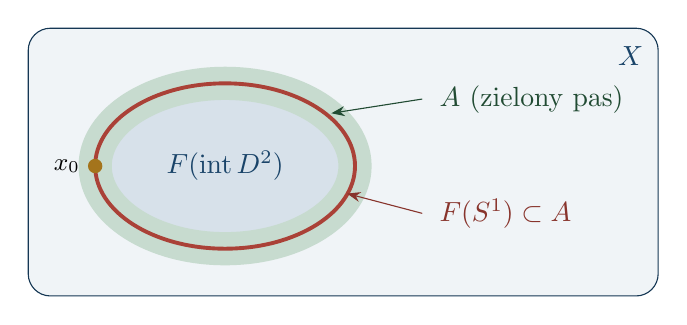
\begin{tikzpicture}[>=Stealth,line cap=round,line join=round]
 \filldraw[rounded corners=8pt,fill=manifoldblue!7,draw=manifoldblue!60!black]
  (0,0) rectangle (8,3.4);
 \fill[manifoldblue!18] (2.5,1.65) ellipse (1.65 and 1.05);
 \draw[manifoldgreen!28,line width=12pt] (2.5,1.65) ellipse (1.65 and 1.05);
 \draw[manifoldred,line width=1.4pt] (2.5,1.65) ellipse (1.65 and 1.05);
 \fill[manifoldgold!80!black] (.85,1.65) circle(2.6pt);
 \node[left,font=\small] at (.78,1.65) {$x_0$};
 \node[manifoldblue!75!black] at (2.5,1.65) {$F(\operatorname{int}D^2)$};
 \node[anchor=west,manifoldgreen!60!black] at (5.1,2.5) {$A$ (zielony pas)};
 \draw[->,manifoldgreen!60!black] (5,2.5)--(3.85,2.32);
 \node[anchor=west,manifoldred!80!black] at (5.1,1.05) {$F(S^1)\subset A$};
 \draw[->,manifoldred!80!black] (5,1.05)--(4.05,1.3);
 \node[manifoldblue!75!black] at (7.65,3.05) {$X$};
\end{tikzpicture}
\caption{Przykład odwzorowania względnego $(D^2,S^1,*)\to(X,A,x_0)$.
Czerwony obraz brzegu leży w zielonym pasie $A$, podczas gdy
obraz wnętrza dysku może wyjść poza $A$. W ogólnej definicji
nie wymaga się różnowartościowości $F$.}
\label{fig:pi-wzgledny-dysk}
\end{figure}

\begin{twierdzenie}[Długi ciąg homotopii pary]
\label{thm:les-pi}
Dla $x_0\in A\subseteq X$ otrzymujemy
naturalny ciąg
\begin{equation}\label{eq:les-pi}
 \cdots\to\pi_n(A,x_0)\xrightarrow{i_*}
 \pi_n(X,x_0)\xrightarrow{j_*}
 \pi_n(X,A,x_0)\xrightarrow{\partial}
 \pi_{n-1}(A,x_0)\xrightarrow{i_*}
 \pi_{n-1}(X,x_0)\to\cdots .
\end{equation}
Jest on dokładny: obraz każdej
strzałki to jądro następnej.
Odwzorowanie $\partial$ ogranicza
reprezentujący dysk do jego
wyróżnionej ściany $B$.
Na końcu ciągu występują
zbiory $\pi_1(X,A,x_0)$ i
$\pi_0(A),\pi_0(X)$; dokładność
oznacza tam przeciwobraz
wyróżnionego elementu.
\end{twierdzenie}
\begin{proof}
W modelu kostkowym $i_*$ jest
włączeniem $A\to X$, a $j_*$
traktuje odwzorowanie z całym brzegiem
w $x_0$ jako odwzorowanie względne.
Wzór $\partial[F]=[F|_B]$
jest poprawny, ponieważ
$\partial B\subset J$ i
$F(J)=x_0$. Homotopia
względna ogranicza się
do homotopii opartych
odwzorowań na $B$, więc
$\partial$ nie zależy
od reprezentanta.

Sprawdźmy trzy kolejne miejsca.
\emph{W $\pi_n(X)$.} Jeśli $f$ ma cały obraz w $A$, homotopia
$f_t(s',r)=f(s',(1-t)r+t)$ jest względną homotopią do stałej;
tutaj $s'\in I^{n-1}$, a $r$ jest ostatnią współrzędną.
Odwrotnie, niech $H(s',r,t)$ będzie względną homotopią
od $f$ do stałej. Ściana $g(s',t)=H(s',0,t)$ leży w $A$
i ma cały brzeg w $x_0$, więc reprezentuje element $\pi_n(A)$.
W kwadracie $(r,t)$ porównujemy drogi od $(0,0)$ do $(1,1)$:
dolny, a potem prawy bok oraz lewy, a potem górny bok.
Są homotopijne względem końców przez liniową interpolację w kwadracie.
Po złożeniu z $H$ dają odpowiednio $f$ i $g$ ze stałym dodatkowym
odcinkiem; na brzegu współrzędnych $s'$ wszystko pozostaje w $x_0$.
Stąd $[f]=i_*[g]$.

\emph{W $\pi_n(X,A)$.} Dysk
pochodzący z $\pi_n(X)$
ma stały brzeg, więc jego
$\partial$ jest zerem.
Jeśli natomiast brzeg
$F|_B:S^{n-1}\to A$ jest
zerowy w $\pi_{n-1}(A)$,
wybieramy jego wypełnienie
przez $D^n\to A$. Sklejenie
tego wypełnienia z $F$
wzdłuż wspólnego brzegu
daje oparte odwzorowanie
$S^n=D^n\cup_{S^{n-1}}D^n\to X$.
Po zapomnieniu drugiego
dysku jego obraz względny
jest klasą $[F]$.

\emph{W $\pi_{n-1}(A)$.} Brzeg
dysku względnego wypełnia
się w $X$, więc ginie
po włączeniu do $X$.
Jeśli oparte odwzorowanie
$S^{n-1}\to A$ jest
zerowe w $\pi_{n-1}(X)$,
jego homotopia do odwzorowania
stałego wyznacza wypełnienie
$D^n\to X$ i tym samym
klasę względną, której
brzeg jest daną klasą.
Te trzy rachunki powtarzają się w sąsiednich stopniach.
Na końcu ciągu element $\pi_1(X,A,x_0)$ jest drogą
od pewnego $a\in A$ do $x_0$, a $\partial$ przypisuje mu
składową $a$ w $A$. Trafia ona do wyróżnionej składowej $X$.
Odwrotnie, punkt tej składowej można połączyć drogą z $x_0$.
Jeśli $a$ leży w składowej $x_0$ już w $A$, dopinamy drogę
z $x_0$ do $a$ w $A$ i otrzymujemy pętlę w $X$ reprezentującą
daną klasę względną. To dowodzi dokładności także dla zbiorów wskazanych.
Wszystkie konstrukcje zachowują się przy składaniu z odwzorowaniem par,
co daje naturalność ciągu.
\end{proof}

\begin{definicja}[Spójność homotopijna]
\index{spojnosc homotopijna@Spójność homotopijna}
\label{def:spojnosc-homotopijna}
Przestrzeń $X$ jest
\emph{$r$-spójna} ($r\geq0$),
jeśli jest łukowo spójna
i $\pi_i(X)=0$ dla $1\leq i\leq r$.
W szczególności $1$-spójna
oznacza jednospójną.
Para $(X,A)$ jest
\emph{$r$-spójna}, jeśli
każda składowa łukowa $X$
spotyka $A$ oraz
$\pi_i(X,A)=0$ dla
$1\leq i\leq r$ przy każdym wyborze punktu bazowego w $A$
(w stopniu $1$ jest to
trywialność zbioru
z wyróżnioną klasą).
\end{definicja}

Dokładność~\eqref{eq:les-pi}
pokazuje, że dla $r$-spójnej
pary włączenie $A\hookrightarrow X$
jest izomorfizmem na
$\pi_i$ dla $i<r$ oraz
surjekcją na $\pi_r$.
Wymiar komórek CW pozwoli
za chwilę uzyskać takie
zanikanie bez liczenia odwzorowań
pojedynczo.

\section{Homotopie na komórkach CW}
\label{sec:pi-n-cw}

W rozdziale o homologii komórki dawały
generatory grup łańcuchów. W homotopii
ich wymiary pozwalają \emph{usuwać
przeszkody do deformacji}. Żeby
deformować jedną komórkę bez psucia
tego, co zrobiliśmy na jej brzegu,
potrzebujemy przedłużania homotopii.

\begin{lemat}[Zwarte obrazy i homotopie w CW]
\label{lem:zwartosc-cw-pi}
Każdy zwarty podzbiór kompleksu CW leży w skończonym podkompleksie.
Ponadto odwzorowanie $H:X\times I\to Y$ jest ciągłe, jeśli jego złożenia
z każdym $\chi_\alpha\times\id_I:D^{d_\alpha}\times I\to X\times I$
są ciągłe, gdzie $\chi_\alpha$ są odwzorowaniami charakterystycznymi komórek.
\end{lemat}
\begin{proof}
Gdyby zwarty zbiór $C$ spotykał nieskończenie wiele otwartych komórek,
wybralibyśmy z każdej z nich jeden punkt $c_\alpha\in C$.
Każda domknięta komórka spotyka tylko skończenie wiele spośród tych punktów.
Każdy podzbiór $E$ zbioru wybranych punktów ma więc domknięty
przeciwobraz przez każde odwzorowanie charakterystyczne: jest to skończona
suma przeciwobrazów punktów w przestrzeni Hausdorffa.
Topologia słaba mówi, że $E$ jest domknięty w $X$.
Zatem zbiór wszystkich $c_\alpha$ jest domkniętym, dyskretnym
podzbiorem zwartego $C$, co jest niemożliwe, jeśli jest nieskończony.
Do skończenie wielu spotkanych komórek dołączamy ich ściany;
warunek skończoności domknięć i malejące wymiary dają skończony podkompleks.

Topologia słaba oznacza, że surjekcja
$q:\bigsqcup_\alpha D^{d_\alpha}\to X$ jest ilorazowa.
Iloczyn dowolnego odwzorowania ilorazowego $q:E\to X$ z $\id_I$ też jest ilorazowy.
Aby to sprawdzić, niech przeciwobraz $W\subseteq X\times I$ będzie otwarty.
Dla $(x,t)\in W$ wybieramy zwarte otoczenie $J$ punktu $t$ w $I$
takie, że $\{x\}\times J\subset W$. Zbiór
$V=\{y:\{y\}\times J\subset W\}$ ma otwarty przeciwobraz przez $q$:
dla każdego $e$ nad $V$ skończone pokrycie zwartego $J$
prostokątami zawartymi w przeciwobrazie $W$ daje otoczenie $e$
o tej samej własności. Stąd $V$ jest otwarty i
$V\times\operatorname{int}_I J\subseteq W$ jest otoczeniem $(x,t)$.
To dowodzi tezy o iloczynie, a więc także kryterium ciągłości $H$.
\end{proof}

Z lematu wynika również rozszerzenie homologii komórkowej
z Rozdziału~\ref{ch:homologia-przestrzeni} na dowolne CW i pary CW.
Dla pary skończonych CW definiujemy najpierw
$C_\bullet^{\mathrm{CW}}(X,A)=C_\bullet^{\mathrm{CW}}(X)/C_\bullet^{\mathrm{CW}}(A)$:
jest to kompleks wolny na komórkach spoza $A$, z brzegiem modulo komórki $A$.
Krótki ciąg tych kompleksów daje długi ciąg homologii.
Naturalne porównanie ze zwykłym ciągiem pary i lemat pięciu
przenoszą izomorfizmy dla $A,X$ na grupy względne.
Każdy singularny łańcuch, jego brzeg oraz świadectwo homologiczności
są skończonymi sumami odwzorowań zwartych sympleksów, więc mieszczą się
w skończonym podkompleksie. Cykl pochodzi z takiego podkompleksu,
a relacja między cyklami jest już prawdziwa w pewnym większym,
również skończonym. Tak samo jest dla skończonych sum komórek
i dla par: przecięcie skończonego podkompleksu z podkompleksem $A$
jest skończonym podkompleksem. Izomorfizmy dla modeli skończonych
są zgodne z włączeniami, bo pochodzą z naturalnych ciągów par.
Przechodzą więc na izomorfizmy dla całego CW.
Grupy łańcuchów komórkowych są przy tym \emph{sumami prostymi},
a nie iloczynami: każda kombinacja nadal ma skończony nośnik.

\begin{lemat}[Przedłużanie homotopii dla par CW]
\label{lem:hep-cw}
Niech $A\subseteq X$ będzie podkompleksem
CW. Jeśli $f:X\to Y$ i homotopia
$h:A\times I\to Y$ spełniają
$h(a,0)=f(a)$, to istnieje
$H:X\times I\to Y$ takie, że
$H(x,0)=f(x)$ oraz $H|_{A\times I}=h$.
W szczególności homotopię
zadaną na brzegu dołączonego
dysku można przedłużyć do
całego dysku.
\end{lemat}
\begin{proof}
Najpierw rozważmy jedną komórkę
$D^k$, której brzeg $S^{k-1}$
leży w już zbudowanej części.
Na
\[
 (D^k\times\{0\})\cup
 (S^{k-1}\times I)
\subset D^k\times I
\]
mamy dane: $f$ na dole
i homotopię $h$ na boku.
Ta podprzestrzeń jest
retraktem całego cylindra.
Można to zobaczyć jawnie:
pisząc $r=\|x\|$ i
\[
 \lambda(x,t)=
 \min\left\{\frac1r,\frac2{2-t}\right\},
 \qquad
 R(x,t)=\bigl(\lambda x,\,
                  2-\lambda(2-t)\bigr),
\]
przy $r=0$ przyjmujemy
$1/r=+\infty$. Dla $r\leq1/2$ minimum wynosi $2/(2-t)$,
więc wzór jest ciągły także przy $r=0$. Wartość
$R(x,t)$ leży albo na boku
$\|\lambda x\|=1$, albo
na dole z drugą współrzędną
równą $0$. Jeśli $t=0$
lub $r=1$, mamy $\lambda=1$,
więc $R$ pozostawia dane
punkty nieruchome.
Złożenie danych z $R$
przedłuża homotopię
na $D^k\times I$.

Dołączajmy teraz komórki
$X\setminus A$ według
wymiarów. Na każdym kroku
stosujemy poprzednią
konstrukcję na wszystkich
dyskach danego wymiaru;
na ich brzegach odwzorowania
już się zgadzają. Ponieważ
topologia CW jest zadana
przez odwzorowania charakterystyczne,
sklejone homotopie są
ciągłe. Dla nieskończenie wielu komórek uzasadnieniem ciągłości
z parametrem czasu jest Lemat~\ref{lem:zwartosc-cw-pi},
zastosowany do wszystkich odwzorowań $D^k\times I\to Y$.
Dla $0$-komórek wybieramy homotopię stałą równą wartości $f$;
wzór na $R$ jest potrzebny dla $k\geq1$.
\end{proof}

\begin{twierdzenie}[Przybliżenie komórkowe]
\label{thm:przyblizenie-komorkowe}
Każde odwzorowanie $f:X\to Y$ kompleksów CW
jest homotopijne z odwzorowaniem
\emph{komórkowym}, czyli takim,
które spełnia
$f(X^k)\subseteq Y^k$ dla
każdego $k$. Jeśli na
podkompleksie $A\subseteq X$
odwzorowanie już jest komórkowe,
homotopię można wybrać
stałą na $A$.
\end{twierdzenie}
\begin{proof}
Wyjaśnijmy lokalny krok geometryczny. Niech
$u:D^k\to Y^m$ wysyła brzeg do $Y^{k-1}$, gdzie $m>k$.
Obraz jest zawarty w skończonym podkompleksie na mocy
Lematu~\ref{lem:zwartosc-cw-pi}. W jednej otwartej $m$-komórce
używamy współrzędnych $\operatorname{int}D^m$ i oznaczamy przez $v$
współrzędnościowy zapis $u$ na otwartym przeciwobrazie tej komórki.
Wybierzmy $0<a<b<c<1$. Zbiór $K=v^{-1}(\overline B_b)$
jest zwarty i leży we wnętrzu $D^k$: obraz $\overline B_b$
jest zwarty i domknięty w przestrzeni Hausdorffa $Y$.
Wybieramy skończone otoczenie wielościenne $P$ zbioru $K$
takie, że $K\subset\operatorname{int}P\subset P\subset v^{-1}(B_c)$.
Można je uzyskać jako sumę domkniętych kostek dostatecznie drobnej siatki
spotykających $K$. Triangulujemy $P$ i przez interpolację wartości $v$
w wierzchołkach dostajemy odcinkowo afiniczne $w$ z
$\|w-v\|<\varepsilon$, gdzie $\varepsilon<\min(b-a,1-c)$.
Istnienie takiego przybliżenia wynika z jednostajnej ciągłości $v$ na $P$:
na każdym małym sympleksie interpolujemy wartości różniące się o mniej niż $\varepsilon$.

Niech $\eta:D^k\to[0,1]$ będzie ciągła, równa $1$ na $K$
i $0$ poza $\operatorname{int}P$. Na $P$ stosujemy homotopię
$v_t=v+t\eta(w-v)$, a poza $P$ nic nie zmieniamy.
Wszystkie wartości pozostają we wnętrzu komórki i homotopia nie rusza brzegu dysku.
Poza $K$ mamy $\|v\|>b$, więc $\|v_t\|>a$.
W $K$ końcowe odwzorowanie jest równe $w$.
Jego obraz jest zawarty w skończonej sumie podprzestrzeni afinicznych
wymiaru co najwyżej $k<m$, która nie zawiera otwartej kuli $B_a$.
Istnieje więc $z\in B_a$ pominięty przez całe nowe odwzorowanie.

Promieniowa retrakcja $D^m\setminus\{z\}$ na $\partial D^m$
zostawia brzeg nieruchomy, więc po sklejeniu komórki daje homotopię
usuwającą jej wnętrze z obrazu $u$. Ciągłość z parametrem czasu
wynika z ilorazowego kryterium z poprzedniego lematu.
Usuwamy kolejno komórki najwyższego wymiaru i schodzimy z wymiarem do $k$.
Pracujemy w skończonym podkompleksie zawierającym obraz i domknięcia
spotkanych komórek, zatem proces kończy się po skończenie wielu krokach.

Zaczynamy od $X^0$:
obraz każdego wierzchołka
przesuwamy do odpowiedniego
wierzchołka w jego składowej
$Y$, a na $A$ niczego
nie zmieniamy. Załóżmy
indukcyjnie, że
$f(X^{k-1})\subseteq Y^{k-1}$.
Dla każdej $k$-komórki
stosujemy lokalny krok
do jej odwzorowania
charakterystycznego:
usuwamy po kolei obrazy
komórek celu o wymiarach
$m>k$, zachowując
jej brzeg. Dostajemy
odwzorowanie tej komórki do
$Y^k$. Dzięki
Lematowi~\ref{lem:hep-cw}
homotopię na dotychczas
zbudowanej części
przedłużamy na całe $X$
i przechodzimy do
następnego wymiaru.
Podane kroki wykonuje
się względnie $A$.
Etapowi wymiaru $k$ przydzielamy przedział
$[1-2^{-k},1-2^{-k-1}]$, a w chwili $1$ bierzemy odwzorowanie końcowe.
Każdy ustalony szkielet pozostaje nieruchomy po zakończeniu swojego etapu.
Na każdym $D^k\times I$ mamy więc skończenie wiele sklejonych homotopii
i stały odcinek końcowy. Lemat~\ref{lem:zwartosc-cw-pi}
zapewnia ciągłość całej homotopii, także w chwili $1$.
\end{proof}

\begin{uwaga}[Przybliżenie w równych wymiarach]
\label{rem:przyblizenie-rowne-wymiary}
Ta sama lokalna konstrukcja dla $k=m$ pozwala wybrać $z\in B_a$
poza obrazami ścian triangulacji $P$ i tych $m$-sympleksów,
na których $w$ ma rząd mniejszy od $m$. Jest to skończona suma
zbiorów o wymiarze mniejszym od $m$. Każdy przeciwobraz $z$
leży wtedy we wnętrzu jednego sympleksu, gdzie $w$ jest afinicznym homeomorfizmem.
Przeciwobrazów jest skończenie wiele, a każdy ma znak wyznacznika $+1$ lub $-1$.
Możemy wokół $z$ wybrać małą kulę, której przeciwobrazy są rozłącznymi
dyskami, odwzorowanymi homeomorficznie na tę kulę.
To wynika również ze zwartości: poza małymi otoczeniami znalezionych
przeciwobrazów obraz omija całe dostatecznie małe otoczenie $z$.
Ten wariant będzie użyty w dowodzie o pierwszych komórkach.
\end{uwaga}

\begin{wniosek}[Szkielet widziany przez $\pi_i$]
\label{cor:pi-szkielety}
Dla kompleksu CW $X$ para
$(X,X^n)$ jest $n$-spójna.
Włączenie $X^n\hookrightarrow X$
daje więc izomorfizm na
$\pi_i$ dla $i<n$
i surjekcję dla $i=n$.
Jeśli $1\leq i<k$, to
$\pi_i(S^k)=0$.
\end{wniosek}
\begin{proof}
Reprezentant klasy
$\pi_i(X,X^n)$ jest
odwzorowaniem $(D^i,\partial D^i)\to
(X,X^n)$, gdzie $i\leq n$.
Najpierw przybliżamy komórkowo odwzorowanie brzegu do $X^n$,
zachowując punkt bazowy, i przedłużamy tę homotopię na dysk
Lematem~\ref{lem:hep-cw}. Dopiero teraz brzeg jest komórkowy,
więc względne przybliżenie na dysku przesuwa cały obraz do
$X^i\subseteq X^n$. Klasa względna znika.
Każda składowa $X$ zawiera wierzchołek: punkt komórki można
połączyć z jej brzegiem i powtarzać to w malejących wymiarach.
To daje także stwierdzenie o składowych i przypadek $n=0$.
Długi ciąg~\eqref{eq:les-pi}
daje twierdzenie o
włączeniu szkieletu.
Sfera $S^k$ ma strukturę CW
z jednym wierzchołkiem
i jedną $k$-komórką,
więc jej $i$-szkielet
jest punktem dla $0\leq i<k$.
Każde oparte odwzorowanie
$S^i\to S^k$ jest
homotopijne do odwzorowania
komórkowego i wtedy
jego obraz jest punktem.
\end{proof}

\begin{stwierdzenie}[Wyższe grupy i nakrycia]
\label{prop:pi-n-nakrycie}
Jeśli $p:\widetilde X\to X$
jest nakryciem, $\widetilde x_0$
leży nad $x_0$, to
\[
 p_*:\pi_n(\widetilde X,\widetilde x_0)
 \xrightarrow{\ \cong\ }
 \pi_n(X,x_0)\qquad(n\geq2).
\]
\end{stwierdzenie}
\begin{proof}
Sfera $S^n$ dla $n\geq2$
jest jednospójna na mocy
Wniosku~\ref{cor:pi-szkielety}
(dla $n=2$ znika $\pi_1$,
a dla większych wymiarów
również). Każde oparte
odwzorowanie $S^n\to X$ podnosi
się więc jednoznacznie
po wskazaniu obrazu
punktu bazowego,
zgodnie z kryterium
z Twierdzenia~\ref{thm:kryterium-podnoszenia}.
Daje to surjektywność $p_*$.
Jeśli dwa podniesienia
po zrzutowaniu są
homotopijne przez odwzorowania oparte,
ich homotopię
$S^n\times I\to X$ podnosimy z kryterium podnoszenia:
$S^n\times I$ jest łukowo i lokalnie łukowo spójna oraz jednospójna,
bo retrahuje się na $S^n$. Ustalamy obraz $(\ast,0)$.
Ścieżka punktu bazowego leży w dyskretnym włóknie, więc jest stała,
a ograniczenie do $S^n\times\{0\}$ jest zadanym podniesieniem.
Jednoznaczność podnoszenia
sprawia, że na końcu
otrzymujemy drugie
podniesienie, ponieważ
oba zgadzają się w
punkcie bazowym.
To daje iniektywność.
\end{proof}

\begin{przyklad}[Okrąg i torus nie mają wyższych $\pi_n$]
\label{prz:pi-torus}
Nakrycia $\R\to S^1$ i
$\R^2\to T^2=S^1\times S^1$
mają ściągalne przestrzenie
całkowite. Zatem dla $n\geq2$
\[
 \pi_n(S^1)=0,\qquad
 \pi_n(T^2)=0.
\]
Jednocześnie
$H_2(T^2)=\Z$ z
Przykładu~\ref{prz:homologia-cw-torus}.
Już tu widać, że w
przestrzeni z nietrywialną
$\pi_1$ wyższa homologia
nie musi być obrazem
wyższej grupy homotopii.
\end{przyklad}

\section{Pierwsze odwzorowanie Hurewicza: od pętli do cykli}
\label{sec:hurewicz-jeden}

\begin{twierdzenie}[Hurewicz w stopniu pierwszym]
\label{thm:hurewicz-h1}
Dla przestrzeni łukowo spójnej $X$
odwzorowanie przypisujące opartej pętli
jej klasę singularnego
$1$-cyklu indukuje naturalny
izomorfizm
\[
 h_1:\pi_1(X,x_0)_{\mathrm{ab}}
 =\pi_1(X,x_0)/
 [\pi_1(X,x_0),\pi_1(X,x_0)]
 \xrightarrow{\ \cong\ }H_1(X;\Z).
\]
\end{twierdzenie}
\begin{proof}
Pętla $\ell:I\to X$ ma
$\partial\ell=[x_0]-[x_0]=0$.
Złożenie dwóch pętli
ma tę samą klasę homologii
co suma ich łańcuchów:
singularny $2$-sympleks, którego boki
przebiegają $\ell_1$, $\ell_2$ i ich złożenie, ma
brzeg $\ell_1+\ell_2-
(\ell_1*\ell_2)$
(z odpowiednią
parametryzacją boków).
Homotopia oparta pętli daje homologiczne cykle przez operator pryzmatyczny
z Twierdzenia~\ref{thm:homotopia-singularna}.
Zatem $[\ell]\mapsto
[\ell]_{H_1}$ jest
homomorfizmem do grupy
abelowej i zabija komutatory.

Skonstruujemy odwrotność.
Dla każdego $x\in X$
wybierzmy drogę $u_x$
od $x_0$ do $x$,
przy czym $u_{x_0}$
jest drogą stałą.
Singularnej krawędzi
$\sigma:x\to y$
przypiszmy w
$\pi_1(X,x_0)_{\mathrm{ab}}$
klasę pętli
\[
 L(\sigma)
 =[u_x*\sigma*\bar u_y].
\]
Niech $\tau:\Delta^2\to X$,
a $x_0',x_1',x_2'$
będą obrazami jej
wierzchołków.
Pętla złożona z boków
$\tau_{01}*\tau_{12}*
\bar\tau_{02}$ jest
zerowa w $\pi_1(X,x_0')$,
gdyż wypełnia ją
sam trójkąt $\tau$.
Po doprowadzeniu jej
do bazy drogami $u_{x_i'}$
otrzymujemy
\[
 L(\partial\tau)
 =L(\tau_{12})-L(\tau_{02})
  +L(\tau_{01})=0
 \quad\text{w }\pi_1(X,x_0)_{\mathrm{ab}}.
\]
Przez liniowość $L$
zeruje więc wszystkie
singularne brzegi
$2$-wymiarowe.
Na cyklach $z\in C_1(X)$
daje homomorfizm
$\bar L:H_1(X)\to
\pi_1(X,x_0)_{\mathrm{ab}}$.

Dla opartej pętli
$\ell$ mamy $L(\ell)=[\ell]$,
więc $\bar Lh_1=\id$.
W drugą stronę,
w homologii
obraz cyklu
$z=\sum m_\sigma\sigma$
rozwija się na
sumę łańcuchów $u_x$, samych krawędzi i $-u_y$,
z dokładnością do brzegów $2$-łańcuchów.
Pojedyncze $u_x$ zwykle nie są cyklami, więc nie przypisujemy
im osobnych klas w $H_1$. Rachunek przeprowadzamy w $C_1(X)/\operatorname{im}\partial_2$.
Tożsamość dla złożenia dróg wynika z trójkąta użytego na początku,
także gdy ich końce są różne; droga odwrotna daje ujemny łańcuch
modulo brzegi, bo droga złożona z własną odwrotnością jest homotopijna do stałej.
Współczynnik przy
każdej pomocniczej
drodze $u_x$ jest
równy minus współczynnikowi
przy $[x]$ w $\partial z$,
a zatem zerowy.
Pozostaje klasa
samego $z$ w $H_1(X)$;
formalnie używamy
homologii złożenia
dróg udowodnionej
na początku. Stąd
$h_1\bar L=\id$
i oba odwzorowania są
odwrotne.
\end{proof}

\begin{przyklad}[Od wolnej grupy do liczby pętli]
Bukiet $r$ okręgów ma
grupę podstawową
$F_r$ z
Przykładu~\ref{prz:pi1-dwa-okregi}
(dla $r=2$ rachunek
podano tam wprost).
Po narzuceniu
przemienności generatorów
$F_r^{\mathrm{ab}}\cong\Z^r$,
zgodnie z
Przykładem~\ref{prz:homologia-bukiet}.
Homologia pamięta tu
liczbę niezależnych
kierunków, ale nie
kolejność, w jakiej
przebywamy pętle.
\end{przyklad}

\section{Twierdzenie Whiteheada}
\label{sec:whitehead}

Równość wszystkich grup $\pi_n$
nie oznacza automatycznie, że
dowolne odwzorowanie przestrzeni
topologicznych ma homotopijną
odwrotność. Dla kompleksów CW
komórki pozwalają jednak
przekształcić informację
o sferach w deformację
całej przestrzeni.

\begin{definicja}[Słaba równoważność homotopijna]
\index{slaba rownowaznosc homotopijna@Słaba równoważność homotopijna}
\label{def:slaba-rownowaznosc}
Odwzorowanie $f:X\to Y$ jest
\emph{słabą równoważnością
homotopijną}, jeśli daje
bijekcję $\pi_0(X)\to\pi_0(Y)$
i dla wszystkich punktów
bazowych $x\in X$ oraz
wszystkich $n\geq1$
izomorfizmy
$f_*:\pi_n(X,x)\to
\pi_n(Y,f(x))$.
\end{definicja}

\begin{lemat}[Ściskanie komórek]
\label{lem:kompresja-cw}
Niech $(K,L)$ będzie parą CW,
a $B\subseteq Y$ niepustą
podprzestrzenią. Załóżmy, że
każda składowa łukowa $Y$ spotyka
$B$ oraz wszystkie grupy
$\pi_k(Y,B,b)$ dla
$k\geq1$ i $b\in B$
są trywialne (dla $k=1$ chodzi o zbiór z wyróżnioną klasą). Wówczas
każde odwzorowanie par
$F:(K,L)\to(Y,B)$
jest homotopijne
\emph{względem $L$}
z odwzorowaniem o obrazie w $B$.
\end{lemat}
\begin{proof}
Dla $0$-komórek $K\setminus L$
wybieramy drogi z ich obrazów
do $B$. Homotopia przesuwa
te obrazy do $B$ i jest
stała na $L$.

Załóżmy, że tak zrobiliśmy
na wszystkich komórkach
o wymiarze mniejszym od $k$.
Dla dołączonej $k$-komórki
odwzorowanie charakterystyczne
daje parę
$(D^k,S^{k-1})\to(Y,B)$.
Przy $k\geq1$ jej klasa
w $\pi_k(Y,B)$ jest zerowa.
Znaczy to, że można
deformować dysk do $B$,
pozwalając początkowo
brzegowi poruszać się w $B$.
Wyjaśnijmy, jak unieruchomić brzeg. Niech
$G:D^k\times I\to Y$ będzie względną homotopią do stałej,
z $G_0=F$ i $G_t(S^{k-1})\subset B$.
Połóżmy $a_t=1-t/2$ i dla $x=ru$ określmy
\[
 K_t(ru)=
 \begin{cases}
 G_t(ru/a_t),&r\leq a_t,\\
 G_{2(1-r)}(u),&a_t\leq r\leq1.
 \end{cases}
\]
Na $r=a_t$ oba wzory dają $G_t(u)$, na $r=1$ mamy stale $F(u)$,
a dla $t=0$ otrzymujemy $F$. Ciągłość przy zanikającym kołnierzu
wynika z ciągłości $G$; dla $t=1$ cały obraz leży w $B$.
Tak dostajemy deformację względem całego brzegu, a nie jedynie
homotopię, która pozwala mu przesuwać się w $B$.
Wykonujemy je na
wszystkich $k$-komórkach
równocześnie.
Lemat~\ref{lem:hep-cw}
przedłuża otrzymaną
homotopię do reszty
$K$, bez ruszania $L$.
Indukcja usuwa obrazy
wszystkich komórek
spoza $L$ z $Y\setminus B$.
Dla nieskończonego CW
przeznaczamy na etap $k$
coraz krótszy przedział
czasu kończący się w $1$.
Każdy ustalony szkielet staje się w końcu nieruchomy.
Ograniczenie do każdej domkniętej komórki, wraz z całym przedziałem czasu,
jest skończonym sklejeniem ciągłych homotopii i stałego końca.
Lemat~\ref{lem:zwartosc-cw-pi} daje ciągłość także w chwili $1$.
\end{proof}

\begin{twierdzenie}[Whitehead]
\label{thm:whitehead}
Słaba równoważność homotopijna
$f:X\to Y$ między kompleksami
CW jest równoważnością
homotopijną. Jeśli
$i:X\hookrightarrow Y$
jest włączeniem podkompleksu
i indukuje izomorfizmy
wszystkich $\pi_n$ oraz
bijekcję na $\pi_0$, to
$X$ jest silnym retraktem
deformacyjnym $Y$.
\end{twierdzenie}
\begin{proof}
Jeśli $X=\varnothing$, bijekcja na składowych wymusza $Y=\varnothing$
i teza jest natychmiastowa. Dalej zakładamy $X\ne\varnothing$.
Zacznijmy od włączenia.
W długim ciągu~\eqref{eq:les-pi}
pary $(Y,X)$ znajdują się
fragmenty
\[
 \pi_n(X)\xrightarrow[\cong]{i_*}
 \pi_n(Y)\longrightarrow
 \pi_n(Y,X)\longrightarrow
 \pi_{n-1}(X)
 \xrightarrow[\cong]{i_*}
 \pi_{n-1}(Y).
\]
Dokładność wymusza
$\pi_n(Y,X)=0$ dla
wszystkich $n\geq2$.
Dla stopnia $1$ warto użyć dróg, ponieważ nie jest to już ciąg grup.
Droga względna od $a\in X$ do $x_0$ ma oba końce w jednej składowej $X$,
gdyż $\pi_0(X)\to\pi_0(Y)$ jest injekcją. Dopinamy drogę
od $x_0$ do $a$ w $X$, otrzymując pętlę w $Y$.
Surjektywność $\pi_1(X)\to\pi_1(Y)$ pozwala zastąpić ją pętlą w $X$.
Każda taka droga jest trywialna względnie $X$, więc $\pi_1(Y,X)$
ma tylko wyróżniony element. Każda składowa $Y$ spotyka $X$,
bo odwzorowanie na $\pi_0$ jest także surjekcją.
Lemat~\ref{lem:kompresja-cw}
zastosowany do
$F=\id_Y:(Y,X)\to(Y,X)$
daje homotopię nieruchomą
na $X$, prowadzącą od
$\id_Y$ do odwzorowania
$r:Y\to X$.
Ponieważ $r|_X=\id_X$,
jest to silna retrakcja
deformacyjna.

Niech teraz $f$ będzie
dowolną słabą równoważnością
CW. Twierdzenie
\ref{thm:przyblizenie-komorkowe}
pozwala zastąpić ją
odwzorowaniem komórkowym $f'\simeq f$.
Zmiana punktu bazowego wzdłuż tej homotopii pokazuje,
że $f'$ nadal jest słabą równoważnością.
Utwórzmy jego
\emph{cylinder odwzorowania}
\[
 M_{f'}=(X\times I)\sqcup Y/
       \bigl((x,1)\sim f'(x)\bigr).
\]
Cylinder ma strukturę CW: poza komórkami $Y$ bierzemy dolne
komórki $e^k\times\{0\}$ i komórki $e^k\times(0,1)$ wymiaru $k+1$.
Brzeg każdej z tych ostatnich składa się z dołu, boków nad
brzegiem $e^k$ i góry odwzorowanej przez $f'$ do $Y^k$.
Komórkowość $f'$ zapewnia zgodność wymiarów, a topologia
ilorazowa i Lemat~\ref{lem:zwartosc-cw-pi} dają topologię słabą.
Dolna kopia $X=X\times\{0\}$ jest więc podkompleksem $M_{f'}$.
Zwijając każdy odcinek
$\{x\}\times I$ do
$f'(x)\in Y$, otrzymujemy
retrakcyjną deformację
$M_{f'}\to Y$.
Złożenie włączenia
$X\hookrightarrow M_{f'}$
z tą retrakcją to $f'$.
Ponieważ $f'_*$ i
retrakcyjne odwzorowanie na $Y$
indukują izomorfizmy
na $\pi_n$, również
włączenie $X\hookrightarrow
M_{f'}$ je indukuje.
Pierwsza część dowodu
ściska więc $M_{f'}$
do $X$. Oznaczmy dolne włączenie przez $j$, włączenie $Y$ do cylindra przez $i$,
a retrakcje na $X,Y$ odpowiednio przez $s,r$.
Wtedy $f'=rj$, a odwrotnością homotopijną jest $g=si$:
$gf'=sirj\simeq sj=\id_X$ oraz $f'g=rjsi\simeq ri=\id_Y$.
Ponieważ $f\simeq f'$, to samo $g$ jest odwrotnością homotopijną $f$.
\end{proof}

\begin{figure}[!htbp]
\centering
\begin{tikzpicture}[>=Stealth,line cap=round,line join=round]
 \fill[manifoldblue!10]
  (0,0)--(4.1,0)--(4.35,2.0)--(.25,2.0)--cycle;
 \draw[manifoldblue!70!black,thick]
  (0,0)--(4.1,0)--(4.35,2.0)--(.25,2.0)--cycle;
 \foreach \x in {.7,1.8,2.9,3.7}{
  \draw[manifoldblue!35] (\x,.07)--({\x+.23},1.94);
 }
 \fill[manifoldgreen!18]
  (-.38,2.0) rectangle (4.86,2.5);
 \draw[manifoldgreen!70!black,thick]
  (-.38,2.0) rectangle (4.86,2.5);
 \node at (2.2,2.25) {$Y$};
 \node[below] at (2.08,0) {$X\times\{0\}$};
 \node[manifoldblue!70!black] at (2.2,1.02)
  {$X\times I$};
 \node[manifoldred!85!black,above]
  at (2.2,2.62) {$(x,1)\sim f'(x)$};
 \draw[->,manifoldred,thick]
  (3.35,1.48)--(3.35,2.2)
  node[midway,right=3pt] {$r$};
 \node[font=\small,align=left,anchor=west,text width=4.8cm]
  at (5.15,1.15)
  {Cylinder zwija się na $Y$.
   Gdy $f'$ jest słabą równoważnością,
   poprzednia część dowodu zwija go
   również na dolną kopię $X$.};
\end{tikzpicture}
\caption{Cylinder odwzorowania zamienia
odwzorowanie $f':X\to Y$ na włączenie
podkompleksu $X\hookrightarrow M_{f'}$.
Rysunek pokazuje mechanizm dowodu
twierdzenia Whiteheada.}
\label{fig:cylinder-whiteheada}
\end{figure}

\begin{uwaga}[Zakres twierdzenia]
Sprawdzenie tylko $\pi_1$
i kilku pierwszych grup
$\pi_n$ nie wystarcza
do zastosowania Whiteheada:
założenie dotyczy
\emph{każdego} $n$.
Również samo podobieństwo
grup homologii dwóch
przestrzeni nie wskazuje
jeszcze odwzorowania, które
mogłoby być równoważnością.
Niżej wyprowadzimy
użyteczne kryterium
homologiczne przy
dodatkowej jednospójności.
\end{uwaga}

\section{Odwzorowanie Hurewicza i pierwszy niezerowy wymiar}
\label{sec:hurewicz-wyzszy}

\begin{definicja}[Odwzorowanie Hurewicza]
\index{odwzorowanie hurewicza@Odwzorowanie Hurewicza}
\label{def:mapa-hurewicza}
Homologia $H_n(S^n;\Z)$
jest izomorficzna z $\Z$
na mocy
Twierdzenia~\ref{thm:homologia-sfer}.
Wybierzmy generatory zgodnie z orientacjami dysków i ich brzegów,
tak aby $\delta[D^n,S^{n-1}]=[S^{n-1}]$.
Dla $n\geq2$ określamy
\[
 h_n:\pi_n(X,x_0)\longrightarrow H_n(X;\Z),
 \qquad h_n([f])=f_*[S^n].
\]
Dla pary $(X,A)$ bierzemy
analogicznie generator
$[D^n,S^{n-1}]
\in H_n(D^n,S^{n-1})$ i
kładziemy
\[
 h_n^{\mathrm{rel}}([F])
 =F_*[D^n,S^{n-1}]
 \in H_n(X,A).
\]
W stopniu $1$ dla przestrzeni używamy homomorfizmu
$\pi_1(X)\to\pi_1(X)_{\mathrm{ab}}\xrightarrow{h_1}H_1(X)$.
Względny homomorfizm określamy tutaj dla $n\geq2$;
zbiór $\pi_1(X,A)$ nie jest w ogólności grupą.
\end{definicja}

Homotopie oparte są w
szczególności zwykłymi
homotopiami odwzorowań, więc
$h_n$ jest dobrze
określone dzięki
Twierdzeniu~\ref{thm:homotopia-singularna}.
Odwzorowanie jest homomorfizmem:
sklejanie dwóch połówek
sfery odpowiada sumie
ich klas fundamentalnych.
Dokładniej, sklejanie jest złożeniem odwzorowania ściskającego równik
$S^n\to S^n\vee S^n$ z $f\vee g$. Odwzorowanie ściskające posyła
generator na sumę dwóch generatorów: rzut na każdy składnik
ma stopień $+1$, co widać z klasy orientacji odpowiedniej półkuli
i naturalności odwzorowania łączącego dla dysku i brzegu.
Względnie używamy kostki podzielonej na dwie połowy w pierwszej współrzędnej.
Po zorientowaniu obu połówek zgodnie z całą kostką ich wewnętrzne
ściany kasują się; obraz łańcucha fundamentalnego jest sumą obu obrazów.
To daje również homomorfizm względny. Naturalność wynika od razu ze składania odwzorowań.

Do dowodu potrzebujemy
przeliczyć grupy homotopii
prostych modeli komórkowych.
Najważniejszy jest
następujący krok: w
pierwszym nowym wymiarze
komórki są niezależne,
a komórki o wymiar
wyższym wprowadzają
relacje.

\begin{lemat}[Pierwsze komórki i ich relacje]
\label{lem:pierwsze-komorki-pi}
Niech $A$ będzie jednospójnym
podkompleksem CW kompleksu $Z$.
Załóżmy, że wszystkie komórki
$Z\setminus A$ mają wymiar
co najmniej $n\geq2$.
Oznaczmy przez $I_n$
zbiór nowych $n$-komórek.
Wtedy
\[
 \pi_n(Z^n\cup A,A)
 \cong\bigoplus_{\alpha\in I_n}\Z[e_\alpha^n]
 \xrightarrow[\cong]{\ h_n^{\mathrm{rel}}\ }
 H_n(Z^n\cup A,A).
\]
Po dołączeniu $(n+1)$-komórek
obie grupy otrzymujemy
z tej wolnej grupy przez
te \emph{same} relacje:
obraz brzegu odwzorowania
dołączającego $S^n\to
Z^n\cup A$. Komórki
o wymiarach co najmniej
$n+2$ nie zmieniają
tych grup.
\end{lemat}
\begin{proof}
Niech $W=Z^n\cup A$ oraz $W'=Z^{n+1}\cup A$.
Przestrzeń $W$ jest jednospójna: do jednospójnego $A$
dołączamy tylko komórki wymiaru co najmniej $2$, co nie tworzy
nowych pętli (lokalny krok przybliżenia komórkowego przesuwa pętlę do $A$).
W szczególności także $\pi_2(W,A)$ jest abelowa, bo z ciągu pary
jest ilorazem abelowej $\pi_2(W)$ przy $\pi_1(A)=0$.
Możemy więc mówić o homomorfizmie z wolnej grupy abelowej
również w przypadku $n=2$.
Po zwinięciu $A$
otrzymujemy bukiet
$\bigvee_{\alpha\in I_n}S^n$.
Względna homologia
$H_n(W,A)$ jest
wolna na komórkach
na mocy
Twierdzenia~\ref{thm:warstwa-komorek}
i rozszerzenia na pary CW po Lemacie~\ref{lem:zwartosc-cw-pi};
to jeszcze nie jest
argument o homotopii,
więc rozpiszmy go
osobno.

Każde odwzorowanie charakterystyczne nowej komórki opieramy w $x_0$
przez dołączenie drogi w $A$ do obrazu wybranego punktu jej brzegu.
Wybór drogi nie zmienia klasy, bo $A$ jest jednospójna.
Tak rozumiemy symbole $[e_\alpha^n]$ po stronie homotopii.
Weźmy teraz odwzorowanie względne
$F:(D^n,S^{n-1},*)\to(W,A,x_0)$.
Zwarty obraz spotyka
tylko skończenie wiele
otwartych komórek.
W każdej z nowych $n$-komórek stosujemy przybliżenie
z Uwagi~\ref{rem:przyblizenie-rowne-wymiary}, nieruchome przy $S^{n-1}$.
Wybieramy regularny punkt $z_\alpha$ poza obrazami ścian triangulacji.
Ma on skończenie wiele przeciwobrazów; na małych otoczeniach
$F$ jest afinicznym homeomorfizmem o znaku $+1$ lub $-1$.
Wybierzmy wokół $z_\alpha$ małą kulę. Jej przeciwobrazy są rozłącznymi
dyskami $D_j$, a poza nimi $F$ omija tę kulę.
Parametryzując $D_j$ przez odwrotność lokalnego odwzorowania afinicznego,
otrzymujemy dokładnie lokalny fragment odwzorowania charakterystycznego;
ujemny znak odpowiada odbiciu pierwszej współrzędnej, czyli odwrotności w grupie. Po usunięciu
środków każda komórka
promieniowo zwija się
na swój brzeg w $A$;
zatem odwzorowanie na dopełnieniu
małych dysków możemy
przesunąć do $A$.
Przedłużamy tę deformację na $D_j$ przez rozszerzanie ich obrazów
od małej kuli do całej komórki, zostawiając zgodność na wspólnych brzegach.
Połączmy małe dyski i punkt bazowy drzewem łuków w ich dopełnieniu.
Rozcinając wzdłuż cienkich pasów tego drzewa, przedstawiamy dysk
jako sumę dysków z doprowadzeniem do bazy; pozostałe części mają obraz w $A$
i reprezentują zero względne. Takie rozcięcie realizuje kolejno
kostkowe dodawanie z Definicji~\ref{def:pi-wzgledne}:
wewnętrzny pas ma obraz w $A$ i można go przesuwać podczas homotopii względnej.
Zmiana drogi doprowadzającej modyfikuje składnik przez pętlę w $A$.
Ponieważ $\pi_1(A)=0$, te zmiany nie wpływają na klasę.
Ostatecznie $[F]$ jest sumą klas charakterystycznych dysków
$e_\alpha^n$, z ich znakami. Każda suma jest skończona.
To dowodzi surjektywności
odwzorowania od wolnej grupy
na nowych komórkach
do $\pi_n(W,A)$.
Obrazy tych generatorów
przez $h_n^{\mathrm{rel}}$
tworzą bazę
$H_n(W,A)$. Gdyby ich
kombinacja dawała
zerową klasę względnej
homotopii, jej obraz
homologiczny również
byłby zerowy; niezależność
bazy wymusza wszystkie
współczynniki równe $0$.
Mamy więc izomorfizm.

Niech teraz dołączamy dyski $D^{n+1}_\beta$, otrzymując $W'$.
Każde odwzorowanie $D^n\to W'$ względnie $A$ przesuwamy do $W$
przez lokalne usuwanie punktów w komórkach wymiaru $n+1$.
Włączenie indukuje więc surjekcję na $\pi_n$.
Relację od $\varphi_\beta:S^n\to W$ rozumiemy jako jej obraz
przez $\pi_n(W)\to\pi_n(W,A)$.
Ich odwzorowania charakterystyczne
dają oczywiste relacje:
brzeg każdego takiego
dysku staje się zerem
w $\pi_n(W',A)$.
Dlaczego nie pojawiają
się inne relacje?
Homotopię względną
między dwoma sumami
$n$-dysków przedstawiamy
na $D^n\times I$.
Uwaga~\ref{rem:przyblizenie-rowne-wymiary}, zastosowana do cylindra
triangulowanego jako $(n+1)$-dysk i nieruchomo na całym jego brzegu,
zapewnia, że przeciwobrazy wybranych punktów $(n+1)$-komórek
są skończonym zbiorem
we wnętrzu $(n+1)$-wymiarowego
cylindra. Usuwamy małe
otoczenia tych punktów.
Pozostała część odwzorowania
omija środki i promieniowo
przesuwa się do $W$.
Na brzegu każdego
usuniętego otoczenia
otrzymujemy, ze znakiem,
odwzorowanie dołączające
odpowiedniej komórki.
Łączymy te otoczenia z brzegiem cylindra drzewem łuków.
Po rozcięciu wzdłuż drzewa zorientowany brzeg pozostałego obszaru
daje różnicę końcowych $n$-dysków oraz sumę nowych sfer brzegowych.
Jego wypełnienie leży w $W$, a pozostałe ściany w $A$,
więc w $\pi_n(W,A)$ otrzymujemy równość różnicy klas z sumą
obrazów $[\varphi_\beta]$, ze znakami lokalnych homeomorfizmów.
Drogi doprowadzające leżą teraz w $W$; nie zmieniają klas,
ponieważ $W$ jest jednospójna. To wyjaśnia, dlaczego dostajemy
zwykłe całkowite kombinacje, bez dodatkowych sprzężeń.
Każda relacja w
$\pi_n(W',A)$
jest więc kombinacją
brzegów dołączonych
komórek.
W homologii to samo
stwierdza wzór
na brzeg komórkowy
\eqref{eq:formula-komorkowa}:
stopnie odwzorowań dołączających
są dokładnie
współczynnikami
tych relacji.

Wreszcie dla $k\geq n+2$
homotopię dysku $D^n$
można przybliżyć
komórkowo, zachowując
brzeg w $A$: jej obraz
nie musi wchodzić
do nowych $k$-komórek.
To samo dotyczy
$(n+1)$-wymiarowej
homotopii, bo $n+1<k$.
Zatem grupy $\pi_n$
nie zmieniają się.
Również względny
kompleks komórkowy
nie zmienia swoich
grup i brzegów
w stopniach $n$ i $n+1$.
\end{proof}

\begin{wniosek}[Zabijanie wybranych klas]
\label{cor:zabijanie-klas-pi}
Niech $Y$ będzie jednospójnym CW i $k\geq2$.
Dołączenie $(k+1)$-komórek wzdłuż klas $a_\beta\in\pi_k(Y)$
zmienia $\pi_k(Y)$ na iloraz przez podgrupę generowaną przez $a_\beta$,
a nie zmienia $\pi_i$ dla $i<k$.
\end{wniosek}
\begin{proof}
Oznaczmy nową przestrzeń przez $V$. Poprzedni lemat z bazą $A=Y$
i pierwszym nowym wymiarem $k+1$ mówi, że
$\pi_{k+1}(V,Y)$ jest wolna na dołączonych komórkach.
Odwzorowanie brzegowe do $\pi_k(Y)$ posyła ich generatory na $a_\beta$.
Niższe grupy względne znikają przez lokalny krok przybliżenia
komórkowego, ponieważ dyski tych wymiarów można przesunąć do $Y$.
Długi ciąg pary daje dokładnie podany iloraz i izomorfizmy w niższych stopniach.
\end{proof}

\begin{uwaga}[O przybliżeniu w lemacie]
Warunek $\pi_1(A)=0$ ma
konkretną rolę: pozwala
jednoznacznie przenosić
lokalne dyski do bazy.
Gdy $A$ nie jest
jednospójna, powstają
przesunięte przez pętle
kopie generatorów.
Wersja względnego
twierdzenia Hurewicza
bez tego warunku
wymaga ilorazu przez
działanie $\pi_1(A)$;
nie utożsamiamy wtedy
bezpośrednio całej
$\pi_n(X,A)$ z
$H_n(X,A)$.
\end{uwaga}

\begin{lemat}[Model bez niższych komórek]
\label{lem:model-wysoko-spojny}
Jeśli kompleks CW $X$
jest $(n-1)$-spójny,
$n\geq2$, to jest
homotopijnie równoważny
kompleksowi $Z$ z
jedną $0$-komórką
i bez komórek
wymiarów $1,\ldots,n-1$.
Odwzorowanie $Z\to X$
można dobrać tak,
by przenosiło
wyróżniony punkt
na $x_0$.
\end{lemat}
\begin{proof}
Zaczynamy od jednej
$0$-komórki $Z^0=\{*\}$
wysłanej do $x_0$.
Ponieważ $\pi_i(X)=0$
dla $i<n$, odwzorowanie to
jest już izomorfizmem
na tych grupach.
Dołączamy do punktu
po jednej $n$-komórce
dla wybranego zbioru
generatorów $\pi_n(X)$.
Każda taka komórka
z brzegiem sklejonym
do punktu jest $S^n$;
odwzorowanie do $X$ definiujemy
na niej reprezentantem
wybranej klasy.
Uzyskujemy surjekcję
na $\pi_n(X)$.

Teraz dla każdego
generatora jądra
$\pi_n(Z^n)\to\pi_n(X)$
dołączamy $(n+1)$-komórkę
wzdłuż reprezentującego
go odwzorowania $S^n\to Z^n$.
Jej obraz w $X$
jest zerowy w $\pi_n(X)$,
więc wybieramy
wypełnienie $D^{n+1}\to X$
i przedłużamy odwzorowanie
$Z\to X$.
Wniosek~\ref{cor:zabijanie-klas-pi}, zastosowany do $Y=Z^n$,
mówi, że dokładnie te relacje zabijają wybrane jądro; w
stopniu $n$ odwzorowanie
staje się izomorfizmem.
Dołączone komórki
nie zmieniają niższych
grup dzięki
Wnioskowi~\ref{cor:pi-szkielety}.

Powtarzamy procedurę
w stopniu $k=n+1,n+2,\ldots$:
komórki $k$-wymiarowe
dołączone do punktu
realizują brakujące
elementy $\pi_k(X)$,
a komórki $(k+1)$-wymiarowe
dołączone wzdłuż klas
z jądra zabijają
dokładnie te klasy.
Dołączenie sfer $S^k$ do punktu daje surjekcję na brakujące klasy
i nie narusza już ustalonych niższych grup: nowy bukiet ma retrakcję
na poprzedni etap, a względne dyski wymiaru $<k$ można przesunąć do niego.
Do zabijania jądra w każdym stopniu stosujemy
Wniosek~\ref{cor:zabijanie-klas-pi} z bazą równą \emph{całemu bieżącemu etapowi}.
Nie wolno tu ponownie traktować punktu jako jedynej bazy pierwszych komórek,
bo wcześniej dołączono już komórki niższych wymiarów.
Odwzorowania dołączające przybliżamy komórkowo, dzięki czemu otrzymujemy strukturę CW;
homotopia takiego odwzorowania nie zmienia jej klasy ani możliwości wypełnienia w $X$.
Wszystkie odwzorowania do $X$ przedłużają się,
bo obrazy odwzorowań
dołączających z jądra
są zerowe w $\pi_k(X)$.
Komórki późniejszego
wymiaru nie naruszają
ustalonych już
izomorfizmów w
niższych stopniach.
Po wykonaniu
wszystkich etapów otrzymujemy CW $Z$.
Odwzorowania sfer i homotopie mają zwarte dziedziny, więc z Lematu~\ref{lem:zwartosc-cw-pi}
każda klasa i każda relacja pojawiają się już w skończonym etapie.
Stabilizacja grup oznacza zatem, że odwzorowanie $Z\to X$
indukuje izomorfizmy
na wszystkich
$\pi_k$ oraz na
$\pi_0$. Twierdzenie
\ref{thm:whitehead}
zamienia tę słabą
równoważność CW
w równoważność
homotopijną.
\end{proof}

\begin{twierdzenie}[Hurewicz: pierwszy niezerowy wymiar]
\label{thm:hurewicz-wyzszy}
Jeżeli $X$ jest
$(n-1)$-spójnym
kompleksem CW,
$n\geq2$, to
\[
 \widetilde H_i(X;\Z)=0
 \quad\text{dla }i<n,
 \qquad
 h_n:\pi_n(X,x_0)
 \xrightarrow{\ \cong\ }H_n(X;\Z).
\]
Izomorfizm jest naturalny:
dla odwzorowania opartego
$f:X\to Y$ odpowiedni
kwadrat z $f_*$ na
homotopii i homologii
jest przemienny.
\end{twierdzenie}
\begin{proof}
Lemat~\ref{lem:model-wysoko-spojny}
pozwala zastąpić
$X$ homotopijnie
równoważnym $Z$
z $Z^{n-1}=\{*\}$.
Homologia i homotopia
nie zmieniają się
przy tej operacji
(Twierdzenia
\ref{thm:homotopia-singularna}
i~\ref{thm:whitehead}).
W kompleksie komórkowym
$Z$ nie ma grup
łańcuchów w
stopniach $1,\ldots,n-1$,
więc
$\widetilde H_i(Z)=0$
dla $i<n$.

Niech
$E_n=\bigoplus_{\alpha\in I_n}
\Z[e_\alpha^n]$.
Z Lematu~\ref{lem:pierwsze-komorki-pi}
dla $A=\{*\}$ mamy
$\pi_n(Z^n)\cong E_n$.
Włączenie
$Z^n\hookrightarrow Z$
jest surjekcją
na $\pi_n$,
a jądrem są relacje
narzucone przez
$(n+1)$-komórki.
Po lewej otrzymujemy
zatem
\[
 \pi_n(Z)
 \cong
 E_n/\langle
   [\varphi_\beta]:
   \varphi_\beta:S^n\to Z^n
   \text{ dołącza }e_\beta^{n+1}
 \rangle.
\]
Po prawej
$\partial_n^{\mathrm{CW}}=0$,
bo $C_{n-1}^{\mathrm{CW}}=0$,
więc
\[
 H_n(Z)
 \cong E_n/
     \operatorname{im}
       \partial_{n+1}^{\mathrm{CW}}.
\]
Obraz $[\varphi_\beta]$
przez $h_n$ jest
klasą brzegową
$(n+1)$-komórki:
jej współczynniki
w bazie $E_n$
to te same stopnie
odwzorowań dołączających
z Twierdzenia
\ref{thm:formula-komorkowa}.
Oba ilorazy są
więc ilorazami
\emph{tej samej}
wolnej grupy przez
\emph{ten sam}
podmoduł.
Ponieważ $h_n$
na generatorach
$[e_\alpha^n]$
przypisuje im
klasy komórkowe
$[e_\alpha^n]$,
jest izomorfizmem.

Na koniec
$h_n(f_*[u])
=(f\circ u)_*[S^n]
=f_*(u_*[S^n])$,
co dowodzi
naturalności.
\end{proof}

\begin{twierdzenie}[Hurewicz względny dla par jednospójnych]
\label{thm:hurewicz-wzgledny}
Niech $(X,A)$ będzie parą CW,
$A\ne\varnothing$ i $A$
jednospójna. Jeśli para
jest $(n-1)$-spójna,
$n\geq2$, to
\[
 H_i(X,A;\Z)=0\quad(i<n),
 \qquad
 h_n^{\mathrm{rel}}:
 \pi_n(X,A,x_0)
 \xrightarrow{\ \cong\ }
 H_n(X,A;\Z).
\]
\end{twierdzenie}
\begin{proof}
Zbudujemy najpierw
model pary bez nowych
komórek poniżej
wymiaru $n$.
Długi ciąg~\eqref{eq:les-pi}
oraz $\pi_i(X,A)=0$
dają izomorfizmy
$\pi_i(A)\to\pi_i(X)$
dla $i<n-1$ i
surjekcję dla
$i=n-1$.
Zaczynamy od
identyczności $A\to A$
oraz włączenia $A\to X$.
Dołączamy $n$-komórki
wzdłuż reprezentantów
jądra
$\pi_{n-1}(A)\to
\pi_{n-1}(X)$.
Każdy taki reprezentant
wypełnia się w $X$,
więc odwzorowanie do $X$
przedłuża się na
nową komórkę.
W długim ciągu
pary nowych komórek
odwzorowanie brzegowe
$\pi_n(Z^n,A)\to
\pi_{n-1}(A)$
posyła każdą
charakterystyczną
$n$-komórkę na
klasę jej odwzorowania
dołączającego.
Lemat~\ref{lem:pierwsze-komorki-pi},
zastosowany do
jednospójnego $A$,
pokazuje, że
te dołączenia
zabijają dokładnie
podgrupę przez
nie generowaną,
czyli wybrane jądro.
W stopniach
niższych niczego
nie zmieniają.
Gdy $n=2$,
wyjściowe $\pi_1(A)$
jest już zerowe
i ten krok nie
wymaga komórek.

Teraz dla $k=n,n+1,\ldots$
postępujemy jak w
dowodzie Lematu
\ref{lem:model-wysoko-spojny}:
dołączamy $k$-komórki
z brzegiem wysłanym
do $x_0$, aby
otrzymać surjekcję
na $\pi_k(X)$,
a potem
$(k+1)$-komórki
wzdłuż generatorów
jądra, aby
otrzymać izomorfizm.
Nigdy nie dołączamy
komórek wymiaru
mniejszego od $n$.
W każdym kroku wniosek o zabijaniu klas stosujemy z bieżącym,
jednospójnym etapem jako bazą. Przybliżamy komórkowo odwzorowania dołączające.
Powstaje odwzorowanie par $F:(Z,A)\to(X,A)$
równe identyczności na $A$, które
indukuje izomorfizmy
wszystkich grup
homotopii przestrzeni
oraz składowych.
Twierdzenie~\ref{thm:whitehead}
zapewnia równoważność
homotopijną $Z\simeq X$.
Porównując długie ciągi
homotopii i homologii
obu par, widzimy
ponadto, że $F$
indukuje izomorfizmy
grup \emph{względnych}:
odwzorowania na wyrazach dotyczących $A$ są identycznością,
a na wyrazach dotyczących $Z,X$ izomorfizmami.
Dla stopni co najmniej $3$ stosujemy lemat pięciu do grup abelowych.
W stopniu $2$ względne grupy są ilorazami $\pi_2(Z)$ i $\pi_2(X)$
przez obrazy $\pi_2(A)$, ponieważ $\pi_1(A)=0$;
to daje izomorfizm bez stosowania lematu pięciu do zbiorów.
Stopień $1$ jest trywialny po obu stronach, bo wszystkie trzy przestrzenie
są jednospójne. Dla homologii stosujemy zwykły lemat pięciu.

W modelu $(Z,A)$
nie ma względnych
łańcuchów komórkowych
w wymiarach $<n$,
więc $H_i(Z,A)=0$
dla $i<n$.
Lemat~\ref{lem:pierwsze-komorki-pi}
oblicza zarówno
$\pi_n(Z,A)$,
jak i $H_n(Z,A)$
jako tę samą
wolną grupę na
$n$-komórkach
modulo te same
relacje od
$(n+1)$-komórek.
Na generatorach
odwzorowanie $h_n^{\mathrm{rel}}$
przypisuje dyskowi
jego klasę orientacji,
więc jest izomorfizmem.
Naturalność
$h_n^{\mathrm{rel}}$
przenosi ten wynik
przez $F$
na parę $(X,A)$.
\end{proof}

\begin{przyklad}[Dysk względem brzegu]
\label{prz:pi-dysk-brzeg}
Dla pary $(D^{n+1},S^n)$
długi ciąg homotopii
i ściągalność dysku
dają w szczególności
\[
 \partial:
 \pi_{n+1}(D^{n+1},S^n)
 \xrightarrow{\ \cong\ }
 \pi_n(S^n)
 \qquad(n\geq1).
\]
Generator po lewej jest reprezentowany przez dysk tożsamościowy,
a jego brzegiem jest
tożsamość sfery.
W homologii dzieje się
to samo na mocy
Twierdzenia~\ref{thm:homologia-sfer};
oba ciągi łączy odwzorowanie
Hurewicza.
\end{przyklad}

\begin{wniosek}[Homologiczne kryterium Whiteheada]
\label{cor:whitehead-homologiczny}
Niech $f:X\to Y$ będzie odwzorowaniem
między jednospójnymi
kompleksami CW.
Jeśli
$f_*:H_i(X;\Z)\to H_i(Y;\Z)$
jest izomorfizmem
dla wszystkich $i$,
to $f$ jest
równoważnością
homotopijną.
\end{wniosek}
\begin{proof}
Zastępujemy $f$
odwzorowaniem komórkowym
homotopijnym z nim
i tworzymy cylinder
$M_f$ z dowodu
Twierdzenia~\ref{thm:whitehead}.
Włączenie
$i:X\hookrightarrow M_f$
ma te same odwzorowania
na homologii co $f$
po złożeniu z
retrakcyjną deformacją
$M_f\to Y$.
Zatem w długim
ciągu homologii
pary $(M_f,X)$
wszystkie grupy
$H_i(M_f,X)$
są zerowe.
Ponieważ $X$
i $M_f\simeq Y$
są jednospójne,
długi ciąg homotopii
daje
$\pi_1(M_f,X)=0$.

Załóżmy, że pewna
wyższa względna
grupa homotopii
nie znika, i weźmy
najmniejsze $n\geq2$
z $\pi_n(M_f,X)\ne0$.
Para jest wtedy
$(n-1)$-spójna,
a $X$ jednospójna.
Twierdzenie
\ref{thm:hurewicz-wzgledny}
dałoby
$H_n(M_f,X)\cong
\pi_n(M_f,X)\ne0$,
sprzeczność.
Wszystkie względne
$\pi_n$ są więc
zerowe, a długi
ciąg homotopii
pokazuje, że
$i$, a zatem $f$,
indukuje izomorfizmy
wszystkich $\pi_n$.
Twierdzenie
\ref{thm:whitehead}
kończy dowód.
\end{proof}

\section{Obliczenia i ograniczenia twierdzeń}
\label{sec:pi-przyklady}

\begin{przyklad}[Pierwsza grupa homotopii sfery]
\label{prz:pi-sfera-hurewicz}
Z Wniosku~\ref{cor:pi-szkielety}
wiemy, że $S^n$
jest $(n-1)$-spójna.
Twierdzenia
\ref{thm:hurewicz-wyzszy}
i~\ref{thm:homologia-sfer}
dają dla $n\geq2$
\[
 \pi_i(S^n)=0\quad(1\leq i<n),
 \qquad
 \pi_n(S^n)\cong\Z.
\]
Tożsamość $S^n\to S^n$
odpowiada generatorowi,
a odwzorowanie $g:S^n\to S^n$
odpowiada liczbie
$\deg g$ z
Definicji~\ref{def:stopien-sfer}.
Zatem oparte $g$ jest homotopijne do tożsamości lub do ustalonego
odbicia sfery zachowującego punkt bazowy odpowiednio wtedy,
gdy stopień wynosi $+1$ lub $-1$.
Odbicie ma stopień $-1$, bo odwraca orientację dysku i jego brzegu.
Dla nieopartego $g$ najpierw przesuwamy obraz wyróżnionego punktu do bazy
i przedłużamy tę homotopię na sferę przez własność HEP.
Jednospójność sfery sprawia, że wybór drogi nie wpływa na wynik. W szczególności
odwzorowanie sfery stopnia
$\pm1$ jest
równoważnością
homotopijną:
wywołuje izomorfizm
na $H_n$ i $H_0$,
a inne grupy homologii
sfery są zerowe,
więc można użyć
Wniosku~\ref{cor:whitehead-homologiczny}.
\end{przyklad}

\begin{przyklad}[Kompleks Moore'a]
\label{prz:moore-hurewicz}
Niech $n\geq2$ i $m\geq2$.
Do $S^n$ dołączmy
jedną $(n+1)$-komórkę
odwzorowaniem stopnia $m$.
Powstała przestrzeń
$M(\Z/m\Z,n)$ ma
kompleks komórkowy
\[
 0\longrightarrow\Z
 \xrightarrow{\;\times m\;}\Z
 \longrightarrow0
\]
w dodatnich stopniach $n+1$ i $n$; ponadto $C_0=\Z$,
a pozostałe grupy łańcuchów są zerowe. Zatem
$H_n(M)=\Z/m\Z$,
$H_{n+1}(M)=0$.
Ponieważ przestrzeń
jest $(n-1)$-spójna,
Hurewicz daje
$\pi_n(M)=\Z/m\Z$.
Intuicja jest
dosłowna: dołączony
dysk czyni
$m$-krotne
owinięcie sfery
zerem w pierwszej
niezerowej grupie.
\end{przyklad}

\begin{przyklad}[Dlaczego potrzeba jednospójności]
\label{prz:rp2-pi2}
Nakrycie antypodalne
$p:S^2\to\mathbb{RP}^2$
indukuje izomorfizm
$\pi_2(S^2)\cong
\pi_2(\mathbb{RP}^2)$
na mocy
Stwierdzenia~\ref{prop:pi-n-nakrycie}.
Zatem
$\pi_2(\mathbb{RP}^2)\cong\Z$.
Tymczasem
$H_2(\mathbb{RP}^2)=0$
z Przykładu~\ref{prz:homologia-rp2},
więc tutaj
$h_2:\Z\to0$
nie jest izomorfizmem.
Przestrzeń rzutowa
nie jest jednospójna:
$\pi_1(\mathbb{RP}^2)=\Z/2\Z$.
To konkretna granica
Twierdzenia~\ref{thm:hurewicz-wyzszy}.
\end{przyklad}

\begin{przyklad}[Bukiet $S^1\vee S^2$]
\label{prz:pi-bukiet-pokrycie}
Przestrzeń
$X=S^1\vee S^2$
ma $\pi_1(X)\cong\Z$.
Jej nakrycie uniwersalne
składa się z prostej
z kopią $S^2$ w każdym
punkcie całkowitym.
Pokrycie otrzymujemy przez przesunięcia prostej o liczby całkowite,
przenoszące jednocześnie $S_k^2$ na $S_{k+1}^2$.
Jego przestrzeń jest jednospójna: każda pętla ma obraz
w skończonym odcinku z dołączonymi skończenie wieloma sferami,
a taka przestrzeń jest jednospójna z van Kampena.
Można obliczyć homologię bez zwijania całej prostej:
mamy wierzchołki w punktach całkowitych, krawędzie między nimi
i po jednej $2$-komórce każdej sfery, dołączonej stale do jej wierzchołka.
Z homologii komórkowej
\[
 H_2(\widetilde X)
 \cong\bigoplus_{k\in\Z}\Z.
\]
Nakrycie nie zmienia
$\pi_2$, a
$\widetilde X$
jest jednospójna,
więc Hurewicz daje
\[
 \pi_2(X)\cong
 \pi_2(\widetilde X)
 \cong\bigoplus_{k\in\Z}\Z,
 \qquad
 H_2(X)\cong\Z.
\]
Każda podniesiona
sfera $S_k^2$
rzutuje się
na tę samą sferę
wewnątrz $X$.
W tych bazach
odwzorowanie Hurewicza
sumuje współczynniki:
$(a_k)_{k\in\Z}
\mapsto\sum_k a_k$.
Homologia traci
informację, którą
z podniesionych
sfer reprezentuje
dana klasa.
\end{przyklad}

\begin{figure}[!htbp]
\centering
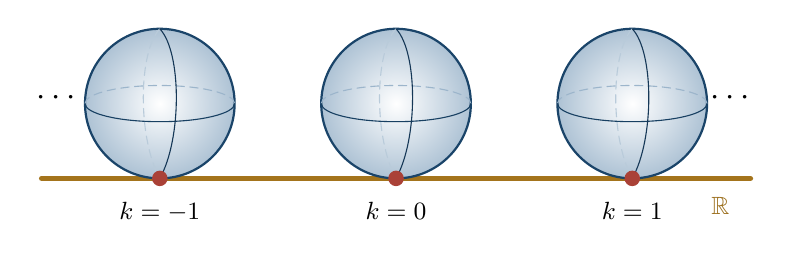
\begin{tikzpicture}[>=Stealth,line cap=round,line join=round]
 \draw[manifoldgold!80!black,line width=2pt]
  (-4.5,0)--(4.5,0);
 \foreach \x/\lab in {-3/{-1},0/{0},3/{1}}{
  \shade[inner color=white,outer color=manifoldblue!37]
   (\x,.95) circle(.95);
  \draw[manifoldblue!75!black,thick]
   (\x,.95) circle(.95);
  \draw[manifoldblue!45,densely dashed,thin]
   ({\x+.95},.95)
   arc[start angle=0,end angle=180,x radius=.95,y radius=.23];
  \draw[manifoldblue!70!black,thin]
   ({\x-.95},.95)
   arc[start angle=180,end angle=360,x radius=.95,y radius=.23];
  \draw[manifoldblue!32,densely dashed,thin]
   (\x,1.9)..controls({\x-.28},1.6)
     and({\x-.28},.5)..(\x,0);
  \draw[manifoldblue!62!black,thin]
   (\x,1.9)..controls({\x+.28},1.6)
     and({\x+.28},.5)..(\x,0);
  \fill[manifoldred] (\x,0) circle(2.8pt);
  \node[below=5pt,font=\small] at (\x,0)
   {$k=\lab$};
 }
 \node[manifoldgold!75!black,font=\small]
  at (4.12,-.35) {$\R$};
 \node[font=\large] at (-4.28,1.02) {$\cdots$};
 \node[font=\large] at (4.28,1.02) {$\cdots$};
\end{tikzpicture}
\caption{Fragment nakrycia uniwersalnego
$S^1\vee S^2$: kopia sfery w każdym
punkcie całkowitym nad pętlą okręgu.
Każda sfera daje inny generator
$\pi_2(X)$, ale wszystkie mają
ten sam obraz w $H_2(X)$.}
\label{fig:nakrycie-bukiet-sfer}
\end{figure}

\begin{uwaga}[Który Whitehead?]
Twierdzenie~\ref{thm:whitehead}
dotyczy słabych równoważności
homotopijnych CW.
\emph{Torsja Whiteheada}
jest innym, późniejszym
niezmiennikiem używanym
przy prostej homotopii
i ogólniejszych
twierdzeniach o
kobordyzmach; sama
nazwa nie czyni jej
częścią tego twierdzenia.
\end{uwaga}

\section*{Dalsza droga}
\addcontentsline{toc}{section}{Dalsza droga}
Następny naturalny blok to
formy różniczkowe,
orientacja, całkowanie,
twierdzenie Stokesa
i kohomologia de Rhama.
Po nich rozwiniemy
geometrię riemannowską:
tensor metryczny, koneksję,
symbole Christoffela,
transport równoległy,
geodezyjne, odwzorowanie
wykładnicze, twierdzenie
Hopfa--Rinowa, krzywiznę
i tensory krzywizny,
pola Jacobiego,
twierdzenia porównawcze
oraz twierdzenie
Gaussa--Bonneta.
\emph{Dopiero po tym bloku}
przejdziemy do teorii
Morse'a, uchwytów,
twierdzenia Smale'a
i chirurgii.
Nie wprowadzamy
tych późniejszych
teorii w obecnym rozdziale.

\par\smallskip
{\footnotesize\noindent\emph{Dalsza lektura:}
Allen Hatcher,
\emph{Algebraic Topology},
rozdział 4, §§4.1--4.2,
\url{https://pi.math.cornell.edu/~hatcher/AT/ATch4.pdf},
zawiera pełne rozwinięcie
grup względnych,
przybliżenia komórkowego,
twierdzeń Whiteheada
i Hurewicza.\par}
\clearpage

\chapter{Formy różniczkowe, orientacja i kohomologia de Rhama}
\label{ch:formy-de-rham}
\index{forma rozniczkowa@Forma różniczkowa}

W Rozdziale~\ref{ch:algebra-tensorowa} zbudowaliśmy algebrę
zewnętrzną jednej przestrzeni wektorowej. Teraz wykonamy tę
konstrukcję w każdym punkcie rozmaitości i pozwolimy, by jej
współczynniki zmieniały się gładko. Otrzymamy formy różniczkowe.
Różniczkowanie form, ich całkowanie i twierdzenie Stokesa
połączą rachunek różniczkowy z homologią przestrzeni z
Rozdziału~\ref{ch:homologia-przestrzeni}. Na końcu porównamy
obie teorie kohomologii. Nadal nie potrzebujemy metryki,
koneksji ani krzywizny; tym pojęciom poświęcimy późniejszy blok.

\section{Czym jest forma różniczkowa?}
\label{sec:formy-definicje}

\begin{definicja}[Formy i ich wartości]
\index{formy i ich wartosci@Formy i ich wartości}
\label{def:forma-rozniczkowa}
Niech $M$ będzie gładką rozmaitością wymiaru $n$.
\emph{Formą różniczkową stopnia $k$} na $M$ nazywamy
gładkie pole naprzemiennych form $k$-liniowych:
\[
 \omega_p\in\Lambda^k T_p^*M,
 \qquad \omega\in\Omega^k(M)
 :=\Gamma(\Lambda^k T^*M).
\]
Przy $k=0$ jest to funkcja gładka,
$\Omega^0(M)=C^\infty(M)$; dla $k>n$ otrzymujemy
$\Omega^k(M)=0$. Przyjmujemy też $\Omega^k(M)=0$ dla $k<0$.
Na rozmaitości z brzegiem gładkość
oznacza lokalne przedłużenie współczynników do
otwartego otoczenia w $\R^n$.
\end{definicja}

Forma $1$-stopnia mierzy wektor styczny i zwraca liczbę.
Forma $2$-stopnia mierzy \emph{zorientowane pole} zadane
parą wektorów; zamiana wektorów zmienia znak.
Jeśli $(U,x)$ jest mapą $x=(x^1,\ldots,x^n)$, to
\begin{equation}\label{eq:forma-lokalna}
 \omega|_U=\sum_{i_1<\cdots<i_k}
 a_{i_1\ldots i_k}\,\dd x^{i_1}\wedge\cdots\wedge\dd x^{i_k},
 \qquad a_I\in C^\infty(U).
\end{equation}
Tutaj $\dd x^i|_p(v)=v(x^i)$ jest kowektorem z
Rozdziału~\ref{ch:rozmaitosci}. Jedyność współczynników
wynika z bazy algebry zewnętrznej
(Twierdzenie~\ref{thm:wedge-baza}). Zmiana mapy zmienia
współczynniki, lecz nie samą formę.

\begin{przyklad}[Dwie formy na płaszczyźnie]
Na $\R^2$ forma $\alpha=x\,\dd y-y\,\dd x$
przypisuje wektorowi $(u,v)$ liczbę $xv-yu$.
Forma $\omega=\dd x\wedge\dd y$ spełnia
\[
 \omega((u_1,v_1),(u_2,v_2))
 =u_1v_2-v_1u_2.
\]
Jest to wyznacznik: wartość bezwzględna daje pole
równoległoboku, znak zaś jego orientację.
\end{przyklad}

\begin{figure}[!htbp]
\centering
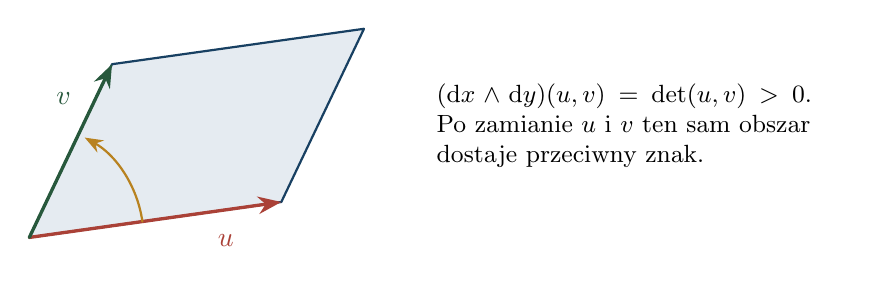
\begin{tikzpicture}[>=Stealth,line cap=round,line join=round]
 \fill[manifoldblue!12] (0,0)--(3.2,.45)--(4.25,2.65)--(1.05,2.2)--cycle;
 \draw[manifoldblue!70!black,thick]
  (0,0)--(3.2,.45)--(4.25,2.65)--(1.05,2.2)--cycle;
 \draw[->,manifoldred,very thick] (0,0)--(3.2,.45)
  node[pos=.78,below=5pt] {$u$};
 \draw[->,manifoldgreen!70!black,very thick] (0,0)--(1.05,2.2)
  node[pos=.8,left=5pt] {$v$};
 \draw[->,manifoldgold!90!black,thick]
  (8:1.45) arc[start angle=8,end angle=61,radius=1.45];
 \node[font=\small,align=left,anchor=west,text width=5.3cm]
  at (5.05,1.42)
  {$(\dd x\wedge\dd y)(u,v)=\det(u,v)>0$.
   Po zamianie $u$ i $v$ ten sam obszar
   dostaje przeciwny znak.};
\end{tikzpicture}
\caption{Forma $\dd x\wedge\dd y$ daje pole ze znakiem
w standardowych współrzędnych płaszczyzny. Ogólna $2$-forma
przypisuje liczbę parze wektorów bez wyboru metryki;
nie musi być euklidesowym polem ich równoległoboku.}
\label{fig:forma-zorientowane-pole}
\end{figure}

\section{Iloczyn zewnętrzny, cofnięcie i różniczka}
\label{sec:formy-dzialania}

\begin{stwierdzenie}[Działania punkt po punkcie]
\label{prop:formy-wedge-pullback}
Dla $\alpha\in\Omega^k(M)$ i $\beta\in\Omega^\ell(M)$
iloczyn $\alpha\wedge\beta\in\Omega^{k+\ell}(M)$
otrzymujemy, biorąc iloczyn zewnętrzny w każdym
$T_p^*M$. Zachodzi $\alpha\wedge\beta
=(-1)^{k\ell}\beta\wedge\alpha$.
Jeżeli $F:M\to N$ jest gładkie, to \emph{cofnięcie}
$F^*:\Omega^k(N)\to\Omega^k(M)$ ma wzór
\begin{equation}\label{eq:pullback-formy}
 (F^*\omega)_p(v_1,\ldots,v_k)
 =\omega_{F(p)}(\dd F_pv_1,\ldots,\dd F_pv_k).
\end{equation}
Spełnia $(G\circ F)^*=F^*G^*$ i
$F^*(\alpha\wedge\beta)=F^*\alpha\wedge F^*\beta$.
\end{stwierdzenie}
\begin{proof}
Gładkość iloczynu w mapie wynika z faktu, że jego
współczynniki są sumami iloczynów gładkich $a_I,b_J$;
przemienność z odpowiednim znakiem jest własnością
algebry zewnętrznej z Rozdziału~\ref{ch:algebra-tensorowa}.
Wzór~\eqref{eq:pullback-formy} jest wieloliniowy i
naprzemienny, a w mapach używa pochodnych współrzędnych
$F$, więc wyznacza formę gładką. Reguła łańcucha
$\dd(G\circ F)_p=\dd G_{F(p)}\circ\dd F_p$
daje własność złożenia. Iloczyn zewnętrzny definiuje
się sumą wartości na przestawionych argumentach; podstawienie
do niej tych samych $\dd F_pv_i$ dowodzi ostatniej równości.
\end{proof}

W szczególności $F^*(\dd y^j)=\dd(y^j\circ F)$.
Jeżeli $F:\R^2\to\R^2$, $F(u,v)=(u^2,v+u)$,
to $F^*(\dd x\wedge\dd y)
=\dd(u^2)\wedge\dd(v+u)=2u\,\dd u\wedge\dd v$.
Współczynnik $2u$ jest wyznacznikiem macierzy Jacobiego
i rejestruje także odwrócenie orientacji przy $u<0$.

\begin{twierdzenie}[Różniczka zewnętrzna]
\label{thm:formy-d}
Istnieje dokładnie jedna rodzina $\R$-liniowych
operatorów $\dd:\Omega^k(M)\to\Omega^{k+1}(M)$
o następujących własnościach:
\begin{enumerate}[leftmargin=*]
\item dla funkcji $f$ forma $\dd f$ jest jej różniczką;
\item $\dd(\alpha\wedge\beta)=\dd\alpha\wedge\beta
 +(-1)^k\alpha\wedge\dd\beta$, gdy $\deg\alpha=k$;
\item $\dd^2=0$.
\end{enumerate}
W mapie jej wzór jest szczególnie prosty:
\begin{equation}\label{eq:zewnetrzna-lokalnie}
 \dd\!\left(\sum_I a_I\,\dd x^I\right)
  =\sum_I\sum_j\frac{\partial a_I}{\partial x^j}
     \dd x^j\wedge\dd x^I,
 \qquad \dd x^I=\dd x^{i_1}\wedge\cdots\wedge\dd x^{i_k}.
\end{equation}
Dla każdego gładkiego $F:M\to N$ zachodzi
$F^*\dd\omega=\dd(F^*\omega)$.
\end{twierdzenie}
\begin{proof}
Najpierw sprawdźmy lokalność dowolnego operatora spełniającego
podane warunki. Jeśli $\omega$ znika w otoczeniu $p$, wybierzmy
gładką funkcję $\chi$, równą $1$ blisko $p$, z nośnikiem
w tym otoczeniu. Taką pojedynczą funkcję buduje się w mapie
z $e^{-1/t}$, jak w dowodzie Twierdzenia
\ref{thm:podzial-jednosci-formy}; nie wymaga to różniczki form.
Ponieważ $\chi\omega=0$, reguła Leibniza daje w $p$
$0=\dd(\chi\omega)_p=(\dd\omega)_p$.
Operator zależy więc tylko od formy w otoczeniu punktu.
Lokalne funkcje i formy możemy pomnożyć przez taką funkcję
odcinającą i przedłużyć przez zero; wynik różniczkowania
blisko $p$ nie zależy od przedłużenia.

Każda forma lokalnie jest sumą wyrazów $a_I\dd x^I$.
Możemy już stosować warunki do lokalnych współrzędnych.
Ponieważ $\dd(\dd x^i)=\dd^2x^i=0$,
reguła Leibniza \emph{wymusza} wzór
\eqref{eq:zewnetrzna-lokalnie}; mamy więc jednoznaczność.
Zdefiniujmy operator tym wzorem. Po powtórnym użyciu
otrzymujemy współczynniki
$(\partial_{x^j}\partial_{x^h}a_I)
\dd x^j\wedge\dd x^h\wedge\dd x^I$.
Wyrazy z $(j,h)$ i $(h,j)$ znoszą się, gdyż pochodne
mieszane są równe, a iloczyn zewnętrzny zmienia znak.
Stąd $\dd^2=0$.

Dla dwóch wyrazów $a\dd x^I$ i $b\dd x^J$
zwykła reguła iloczynu $\dd(ab)=a\dd b+b\dd a$
oraz przestawienie $\dd b$ przez $k$ czynników
$\dd x^I$ dają dokładnie znak $(-1)^k$.
Liniowość rozszerza to na sumy.
Sprawdźmy zgodność na przecięciu map. Cofnięcie przez
zmianę współrzędnych zachowuje $\dd f$ dzięki regule
łańcucha i zachowuje $\wedge$ z poprzedniego
stwierdzenia. Zatem dwa lokalne wzory, obliczone po obu
stronach zmiany współrzędnych, są równe na generatorach
$f,\dd x^i$, a przez regułę Leibniza na wszystkich formach.
Wzory sklejają się w globalny operator. Ten sam argument
dla dowolnego $F$ daje $F^*\dd=\dd F^*$.
\end{proof}

\begin{przyklad}[Rachunek na $\R^3$]
Jeżeli $\alpha=P\,\dd x+Q\,\dd y+R\,\dd z$, to
\[
 \dd\alpha=(Q_x-P_y)\,\dd x\wedge\dd y
 +(R_x-P_z)\,\dd x\wedge\dd z
 +(R_y-Q_z)\,\dd y\wedge\dd z.
\]
Dla $\beta=P\,\dd y\wedge\dd z
+Q\,\dd z\wedge\dd x+R\,\dd x\wedge\dd y$
otrzymujemy $\dd\beta=(P_x+Q_y+R_z)
\dd x\wedge\dd y\wedge\dd z$.
Są to wyrażenia występujące w klasycznych wzorach na rotację
i dywergencję. Utożsamianie tu pól wektorowych z formami
korzysta ze standardowej struktury euklidesowej $\R^3$;
sama różniczka zewnętrzna na $M$ nie wymaga metryki.
\end{przyklad}

\begin{definicja}[Kontrakcja i pochodna Liego]
\index{kontrakcja i pochodna liego@Kontrakcja i pochodna Liego}
\label{def:formy-kontrakcja-lie}
Dla pola wektorowego $X$ operator
$\iota_X:\Omega^k(M)\to\Omega^{k-1}(M)$ określamy przez
\[
 (\iota_X\omega)_p(v_1,\ldots,v_{k-1})
 =\omega_p(X_p,v_1,\ldots,v_{k-1}),
 \qquad \iota_Xf=0.
\]
Jeśli $M$ ma brzeg, w definicji przez dwustronny przepływ
zakładamy, że $X$ jest styczne do $\partial M$.
Jeśli $\Phi_t$ jest lokalnym przepływem $X$ z
Rozdziału~\ref{ch:pola}, kładziemy
$\Lie_X\omega=\left.\frac{\dd}{\dd t}\right|_{t=0}\Phi_t^*\omega$.
\end{definicja}

\begin{twierdzenie}[Wzór Cartana]
\label{thm:cartan-formy}
Dla każdej formy $\omega$ mamy
\begin{equation}\label{eq:cartan-formula}
 \boxed{\ \Lie_X\omega=\dd(\iota_X\omega)
       +\iota_X(\dd\omega)\ }.
\end{equation}
Ponadto $\Lie_X\dd=\dd\Lie_X$ oraz
$\iota_X(\alpha\wedge\beta)=
(\iota_X\alpha)\wedge\beta
+(-1)^{\deg\alpha}\alpha\wedge\iota_X\beta$.
\end{twierdzenie}
Dla pola niestycznego do brzegu prawa strona wzoru Cartana
nadal określa gładką formę. Możemy nią zdefiniować
$\Lie_X\omega$ na brzegu: jest to przedłużenie pochodnej
Liego z wnętrza, niezależne od przedłużeń w mapach.
Nie zakładamy wówczas istnienia dwustronnego przepływu w $M$.
\begin{proof}
Ostatnia równość wynika wprost z definicji iloczynu
zewnętrznego: po wstawieniu $X$ w pierwsze miejsce
może on wejść do pierwszej grupy argumentów lub,
po przejściu przez $\deg\alpha$ argumentów, do drugiej.
Ponieważ $\Phi_t^*$ zachowuje iloczyn zewnętrzny,
$\Lie_X$ jest derywacją stopnia $0$ algebry form.
Prawa strona~\eqref{eq:cartan-formula} również nią jest:
rozwijamy oba składniki na $\alpha\wedge\beta$
regułami dla $\dd$ i $\iota_X$; wyrazy mieszane mają
przeciwne znaki i znoszą się.

Wystarczy zatem porównać obie strony na lokalnych
generatorach $f,\dd x^i$. Dla funkcji lewa strona to
$Xf$, a prawa to $\iota_X\dd f=\dd f(X)=Xf$.
Dla $\dd x^i$ lewa strona wynosi
$\dd(\Lie_Xx^i)=\dd(Xx^i)$, gdyż cofnięcie
komutuje z $\dd$; prawa wynosi
$\dd(\iota_X\dd x^i)+\iota_X\dd^2x^i
=\dd(Xx^i)$. Wzór obowiązuje więc dla
każdej sumy wyrazów $f\,\dd x^I$ i globalnie.
Wreszcie, z $\dd^2=0$ dostajemy
$\dd\Lie_X=\dd\iota_X\dd
=\Lie_X\dd$.
\end{proof}

\begin{przyklad}[Pochodna Liego formy]
Na $\R^2$ weźmy $X=\partial_x$ i $\omega=x\,\dd y$.
Przepływ przesuwa punkty poziomo, więc
$\Phi_t^*\omega=(x+t)\dd y$ oraz
$\Lie_X\omega=\dd y$. Ze wzoru Cartana:
$\iota_X\omega=0$, $\dd\omega=\dd x\wedge\dd y$
i $\iota_X\dd\omega=\dd y$. Oba obliczenia są zgodne.
\end{przyklad}
\section{Lokalne istnienie funkcji pierwotnej}
\label{sec:formy-poincare}

Równość $\dd^2=0$ mówi, że każda forma postaci
$\dd\eta$ jest \emph{zamknięta}. Odwrotność nie zachodzi
globalnie: przeszkodę może stanowić topologia. Lokalnie
przeszkoda znika, co wyjaśnia następujący rachunek.
Dla zamkniętej $1$-formy $\omega$ szukamy \emph{funkcji
pierwotnej} $f$ spełniającej $\omega=\dd f$.
Dla formy stopnia $k>1$ jej odpowiednikiem jest
\emph{forma pierwotna} $\eta$ stopnia $k-1$ z
$\omega=\dd\eta$. Lemat Poincarégo obejmuje
oba przypadki.

\begin{lemat}[Homotopia form]
\label{lem:homotopia-form}
Niech $H:[0,1]\times M\to N$ będzie gładką homotopią
odwzorowań $H_0,H_1$. Przy końcach przedziału, a także
przy narożach iloczynu, gdy $M$ ma brzeg, gładkość
rozumiemy jako gładkie przedłużanie składowych w mapach. Istnieje operator liniowy
$K:\Omega^k(N)\to\Omega^{k-1}(M)$ taki, że
\begin{equation}\label{eq:homotopia-form}
 H_1^*\omega-H_0^*\omega
 =\dd(K\omega)+K(\dd\omega).
\end{equation}
\end{lemat}
\begin{proof}
Dla $k=0$ przyjmujemy $K\omega=0$; poniższy rachunek
obejmuje ten przypadek z $a=0$. Każdą formę na
$[0,1]\times M$ zapisujemy jednoznacznie
w postaci $H^*\omega=\dd t\wedge a(t)+b(t)$,
gdzie $a(t)$ jest rodziną form stopnia $k-1$ na $M$,
a $b(t)$ rodziną form stopnia $k$. Położenie
$K\omega:=\int_0^1 a(t)\,\dd t$ oznacza całkowanie
\emph{współczynników} formy po parametrze; można je
wykonać w każdej mapie, a zgodność na przecięciach
wynika z liniowości zmiany współrzędnych.
Obliczenie różniczki daje
\[
 \dd(H^*\omega)
 =\dd t\wedge(\partial_tb-\dd_Ma)+\dd_Mb.
\]
Ponieważ $H^*\dd\omega=\dd H^*\omega$, współczynniki
przy $\dd t$ mówią, że
$a_{\dd\omega}(t)=\partial_tb(t)-\dd_Ma(t)$.
Po scałkowaniu od $0$ do $1$ otrzymujemy
$K\dd\omega=b(1)-b(0)-\dd_MK\omega$.
Ale $b(i)=H_i^*\omega$ dla $i=0,1$,
więc jest to dokładnie~\eqref{eq:homotopia-form}.
\end{proof}

\begin{twierdzenie}[Lemat Poincarégo]
\label{thm:lemat-poincare-formy}
Niech $U\subset\R^n$ będzie otwarty i gwiaździsty
względem $0$. Jeżeli $k\geq1$ i
$\omega\in\Omega^k(U)$ spełnia $\dd\omega=0$,
to istnieje $\eta\in\Omega^{k-1}(U)$ z
$\omega=\dd\eta$. Każda zamknięta forma stopnia
$0$ jest stała na $U$.
\end{twierdzenie}
\begin{proof}
W Lemacie~\ref{lem:homotopia-form} bierzemy
$H(t,x)=tx$. Dla $k\geq1$ odwzorowanie $H_0$
jest stałe, więc $H_0^*\omega=0$; dla zamkniętej
$\omega$ drugi składnik po prawej stronie
\eqref{eq:homotopia-form} także znika.
Dostajemy $\omega=\dd(K\omega)$.
Jeśli chcemy \emph{obliczyć} formę pierwotną
(dla $k=1$: funkcję pierwotną), to
\begin{equation}\label{eq:poincare-pierwotna}
 (K\omega)_x(v_1,\ldots,v_{k-1})
 =\int_0^1 t^{k-1}
   \omega_{tx}(x,v_1,\ldots,v_{k-1})\,\dd t.
\end{equation}
Istotnie, $\dd H(\partial_t)=x$, podczas gdy
$\dd H(v_i)=tv_i$, skąd $k-1$ czynników $t$.
Gwiaździstość zapewnia, że cały odcinek $tx$ leży w $U$.
Dla $k=0$ warunek $\dd f=0$ mówi, że wszystkie
pochodne kierunkowe znikają. Zatem pochodna
$t\mapsto f(tx)$ jest zerowa i $f(x)=f(0)$.
\end{proof}

\begin{przyklad}[Obliczenie funkcji pierwotnej]
Na $\R^2$ forma $\omega=2xy\,\dd x+x^2\,\dd y$
jest zamknięta, bo
$\dd\omega=(2x-2x)\dd x\wedge\dd y=0$.
Wzór~\eqref{eq:poincare-pierwotna} dla $k=1$ daje
\[
 (K\omega)(x,y)=\int_0^1
 \omega_{(tx,ty)}(x,y)\,\dd t
 =\int_0^1 3t^2x^2y\,\dd t=x^2y.
\]
Zatem $f(x,y)=x^2y$ jest funkcją pierwotną
$1$-formy $\omega$, ponieważ $\omega=\dd f$.
Obliczenie pokazuje mechanizm lematu.
\end{przyklad}

\begin{wniosek}[Niezmienniczość przez homotopię]
\label{cor:de-rham-homotopia}
Odwzorowania gładko homotopijne indukują tę samą
operację cofnięcia na kohomologii de Rhama
z Definicji~\ref{def:de-rham-cohomology}.
\end{wniosek}
\begin{proof}
Jeśli $\dd\omega=0$, wzór~\eqref{eq:homotopia-form}
mówi, że $H_1^*\omega-H_0^*\omega=\dd(K\omega)$.
Różnica jest więc dokładna i obie klasy są równe.
\end{proof}

\section{Podział jedności}
\label{sec:formy-podzial-jednosci}

Przy całkowaniu trzeba scalać dane z wielu map.
Służy do tego wynik, który wyjaśnia także wcześniejsze
użycia funkcji odcinających w skrypcie.

\begin{twierdzenie}[Gładki podział jedności]
\label{thm:podzial-jednosci-formy}
Niech $(U_\alpha)$ będzie otwartym pokryciem rozmaitości
$M$ Hausdorffa i o przeliczalnej bazie. Istnieją
nieujemne funkcje gładkie $(\rho_j)$ o lokalnie skończonej
rodzinie nośników (każdy punkt ma otoczenie spotykające
tylko skończenie wiele nośników) oraz indeksy $\alpha(j)$ takie, że
\[
 \supp\rho_j\subset U_{\alpha(j)},
 \qquad \sum_j\rho_j(p)=1\quad(p\in M).
\]
Każdą $\rho_j$ można wybrać o nośniku zwartym
w jednej dziedzinie mapy zawartej w $U_{\alpha(j)}$.
\end{twierdzenie}
\begin{proof}
Najpierw budujemy jedną funkcję odcinającą.
Jeśli w mapie kula domknięta $\overline B_r$
leży w większej kuli $B_R$, przy czym $0<r<R$
i $\overline B_R$ zawiera się w obrazie mapy,
wybierzmy gładką funkcję $\chi$ zależną tylko
od $\|x\|^2$, równą $1$ na $\overline B_r$,
dodatnią między $r$ i $R$, a zerową poza $B_R$.
Można ją złożyć z funkcji $h(t)=e^{-1/t}$ dla
$t>0$ i $h(t)=0$ dla $t\leq0$; jej gładkość w
$t=0$ wynika z zanikania wszystkich pochodnych
$t^{-a}e^{-1/t}$. Przedłużenie $\chi$ przez $0$
na resztę $M$ jest gładkie, bo nośnik ma zwartą
domkniętą otoczkę wewnątrz mapy. Przy brzegu bierzemy
przecięcia tych kul z półprzestrzenią i ograniczamy do nich
te same funkcje. Wszystkie wnętrza i domknięcia poniżej
rozumiemy w topologii $M$, także przy brzegu.

Z lokalnej zwartości i przeliczalności bazy
konstruujemy wyczerpanie zwartymi zbiorami
$K_1\subset\operatorname{int}K_2\subset\cdots$,
$\bigcup_jK_j=M$ (weźmy kolejno skończone
sumy domkniętych, stosunkowo zwartych kul
obejmujące pierwsze elementy przeliczalnego
pokrycia i powiększmy je przy każdym kroku).
Ustalmy $K_j=\varnothing$ dla $j\leq0$.
Zwarty pas $K_j\setminus\operatorname{int}K_{j-1}$
można pokryć skończenie wieloma małymi kulami
w mapach o domknięciach zawartych jednocześnie
w którymś $U_\alpha$ i w
$\operatorname{int}K_{j+1}\setminus K_{j-2}$.
Wybieramy funkcje odcinające dodatnie na
mniejszych kulach pokrywających pas.
Rodzina tych kul dla wszystkich $j$ jest
lokalnie skończona: otoczenie punktu wewnątrz
pewnego $K_N$ nie spotyka kul pochodzących
z pasów o dostatecznie dużym indeksie.

Niech $\chi_j$ oznaczają wszystkie otrzymane
funkcje. Suma $S=\sum_j\chi_j$ jest lokalnie
skończona, gładka i wszędzie dodatnia, bo
każdy punkt należy do któregoś pasa. Kładziemy
$\rho_j=\chi_j/S$. Wtedy nośniki pozostają
w wybranych kulach i
$\sum_j\rho_j=S/S=1$.
Gdy potrzebujemy funkcji indeksowanych samymi zbiorami
pokrycia, sumujemy $\rho_j$ o tym samym $\alpha(j)$.
Nośnik takiej sumy nadal leży w $U_\alpha$:
lokalnie skończona suma zamkniętych nośników jest
zbiorem domkniętym zawartym w $U_\alpha$.
\end{proof}
\section{Orientowalność i orientacje indukowane}
\label{sec:formy-orientacja}

\begin{definicja}[Orientacja]
\index{orientacja@Orientacja}
\label{def:orientacja-formy}
Dwie uporządkowane bazy $m$-wymiarowej przestrzeni
rzeczywistej $V$, dla $m\geq1$, mają tę samą orientację, jeśli
macierz przejścia ma dodatni wyznacznik.
Powstają dwie klasy baz. Na rozmaitości $M^m$
\emph{orientacja} to gładki wybór takiej klasy w
każdym $T_pM$. Równoważnie jest to klasa
nigdzie niezerowych form $m$-stopnia: formy
$\mu,\nu$ wyznaczają tę samą orientację, jeśli
$\nu=f\mu$ dla gładkiej funkcji $f>0$.
Rozmaitość dopuszczająca taki wybór jest
\emph{orientowalna}; wraz z wyborem orientacji
jest \emph{zorientowana}.
\end{definicja}

W wymiarze $0$ stosujemy opis przez formy najwyższego
stopnia: $\Lambda^0 V^*=\R$, a orientacja jest wyborem
jednej z dwóch półprostych, czyli znaku $+1$ lub $-1$.
Każdemu punktowi rozmaitości dyskretnej przypisujemy taki
znak. Opis przez dwie klasy baz dotyczy tylko $m\geq1$,
gdyż przestrzeń zerowa ma tylko jedną bazę pustą.

Dla $m\geq1$ forma $\mu_p$ określa bazę dodatnią $(v_1,\ldots,v_m)$
przez nierówność $\mu_p(v_1,\ldots,v_m)>0$.
To definicja \emph{znaku}, a nie długości ani pola:
zamiana $\mu$ na $2\mu$ nie zmienia orientacji.
Na każdej spójnej orientowalnej rozmaitości istnieją
dwa wybory globalne, wzajemnie przeciwne.

\begin{twierdzenie}[Trzy opisy orientowalności]
\label{thm:orientacja-atlas-forma}
Dla rozmaitości gładkiej $M^m$ równoważne są
poniższe warunki. W mapach przy brzegu dopuszczamy
obie półprzestrzenie $x^m\geq0$ i $x^m\leq0$;
jest to ta sama struktura gładka, a pozwala stosować
odbicie współrzędnej także w wymiarze $1$.
\begin{enumerate}[leftmargin=*]
\item orientowalność $M$;
\item istnienie atlasu, w którym wszystkie wyznaczniki
      odwzorowań przejścia są dodatnie;
\item istnienie globalnej nigdzie niezerowej formy
      $\mu\in\Omega^m(M)$.
\end{enumerate}
\end{twierdzenie}
\begin{proof}
Dla $m=0$ wszystkie trzy warunki są spełnione:
rozmaitość jest dyskretna, dowolny wybór znaków jest
gładki, a funkcja $1$ jest nigdzie niezerową $0$-formą.
Atlas zerowymiarowy sam nie zapisuje wyboru znaków.
Załóżmy więc $m\geq1$.
Forma $\mu$ wybiera dodatnie bazy w każdym punkcie,
więc (3) daje (1). Jeśli wybór (1) jest ustalony,
zmniejszamy dziedziny map do spójnych otoczeń.
Każdą mapę można w razie potrzeby złożyć z odbiciem
jednej współrzędnej, aby jej standardowa baza była
dodatnia. W nowym atlasie dwie bazy lokalne opisują
tę samą orientację, zatem ich wyznacznik przejścia
jest dodatni: (1) daje (2).

Załóżmy (2). W każdej mapie z tego atlasu lokalna
forma $\mu_j=\dd x_j^1\wedge\cdots\wedge\dd x_j^m$
jest dodatnia. Wybierzmy podział jedności $(\rho_j)$
z Twierdzenia~\ref{thm:podzial-jednosci-formy},
o nośnikach w dziedzinach tych map, i przedłużmy
$\rho_j\mu_j$ przez zero. Suma
$\mu=\sum_j\rho_j\mu_j$ jest lokalnie skończona.
W dowolnym punkcie co najmniej jedno $\rho_j$ jest
dodatnie; wszystkie występujące $\mu_j$ są dodatnimi
wielokrotnościami jednej z nich, bo przejścia
mają dodatni wyznacznik. Suma nie może się
wyzerować. Tak dostajemy (3).
\end{proof}

\begin{stwierdzenie}[Dwa podstawowe sposoby przenoszenia orientacji]
\label{prop:orientacja-iloczyn-pullback}
Jeżeli $F:M\to N$ jest dyfeomorfizmem i $N$ ma
orientację $[\nu]$, to $F^*\nu$ orientuje $M$;
$F$ zachowuje orientację wtedy, gdy zgadza się ona
z uprzednio wybraną orientacją $M$. Jeśli $M^m,N^n$
są zorientowane, orientację $M\times N$ wyznacza
$\pr_M^*\mu\wedge\pr_N^*\nu$.
Po zamianie kolejności czynników znak zmienia się
o $(-1)^{mn}$.
\end{stwierdzenie}
\begin{proof}
Różniczka dyfeomorfizmu jest izomorfizmem, więc
cofnięcie nigdzie niezerowej formy najwyższego stopnia
pozostaje nigdzie niezerowe. Na iloczynie wartości
$\mu\wedge\nu$ na bazie najpierw $TM$, potem $TN$
są dodatnie. Przestawienie $m$ wektorów z pierwszego
czynnika z $n$ wektorami drugiego wymaga $mn$
zamian; każda zmienia znak formy.
\end{proof}

Orientacja brzegu i orientacja regularnego zbioru
poziomicowego są dwiema wersjami tej samej zasady:
\emph{najpierw kierunki normalne, potem styczne}.

\begin{definicja}[Orientacja brzegu: normalna na zewnątrz]
\index{orientacja brzegu normalna na zewnatrz@Orientacja brzegu: normalna na zewnątrz}
\label{def:orientacja-brzegu}
Niech $M^m$ będzie zorientowaną rozmaitością z brzegiem.
Dla $m\geq2$ baza $(v_1,\ldots,v_{m-1})$ przestrzeni $T_p\partial M$
jest dodatnia wtedy i tylko wtedy, gdy
$(n,v_1,\ldots,v_{m-1})$ jest dodatnią bazą $T_pM$
dla dowolnego wektora $n$ skierowanego na zewnątrz.
Wymóg nie zależy od konkretnego $n$: dwa takie wektory
mają dodatnio proporcjonalne składowe poprzeczne,
a dodanie wektora stycznego nie zmienia wyznacznika.
Równoważnie, dla formy $\mu$ reprezentującej orientację,
brzeg orientuje $\iota_n\mu$ ograniczona do $T\partial M$.
Ten opis działa również dla $m=1$: znak w punkcie brzegu
jest znakiem liczby $\mu_p(n)$.
\end{definicja}

\begin{stwierdzenie}[Brzeg jest orientowalny]
\label{prop:brzeg-orientowalny}
Powyższa reguła nadaje $\partial M$ gładką orientację.
Dla standardowej orientacji $[a,b]$ końcowy punkt $b$
ma znak $+1$, a początkowy $a$ ma znak $-1$.
Dla dysku $D^2$ ze standardową orientacją płaszczyzny
brzeg biegnie przeciwnie do ruchu wskazówek zegara.
\end{stwierdzenie}
\begin{proof}
W mapie półprzestrzeni $\{x^m\geq0\}$ kierunek
na zewnątrz to $-\partial_{x^m}$; reguła daje
stały wybór znaku baz współrzędnych stycznych.
Zmiany map zachowują orientację $M$ i wysyłają
kierunek na zewnątrz na kierunek na zewnątrz,
więc uzyskane wybory na przecięciach są zgodne.
W wymiarze $1$ przy $b$ wektor zewnętrzny
$+\partial_t$ jest dodatni, a przy $a$ wektor
$-\partial_t$ ujemny. W dysku przy $(1,0)$
wektor zewnętrzny jest $(1,0)$; aby para była
dodatnia, wektor styczny musi wskazywać $(0,1)$.
Ciągłość przenosi ten kierunek na cały okrąg.
\end{proof}

\begin{figure}[!htbp]
\centering
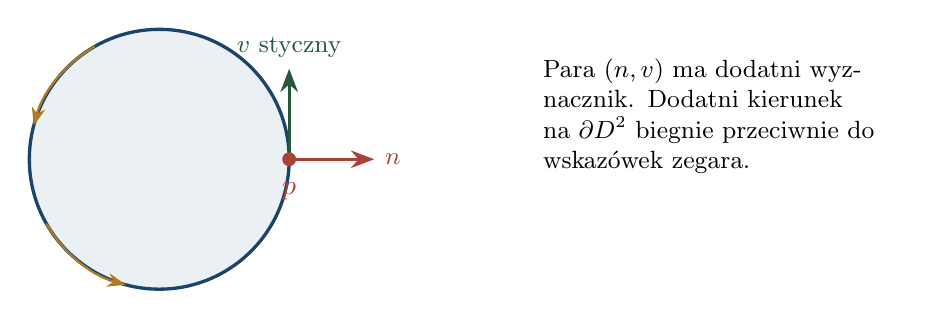
\begin{tikzpicture}[>=Stealth,line cap=round,line join=round]
 \fill[manifoldblue!9] (0,0) circle (1.65);
 \draw[manifoldblue!75!black,line width=1.2pt] (0,0) circle (1.65);
 \draw[->,manifoldred,very thick] (1.65,0)--(2.73,0)
  node[right,font=\small] {$n$};
 \draw[->,manifoldgreen!70!black,very thick] (1.65,0)--(1.65,1.15)
  node[above,font=\small] {$v$ styczny};
 \draw[->,manifoldgold!85!black,thick]
  (210:1.65) arc[start angle=210,end angle=255,radius=1.65];
 \draw[->,manifoldgold!85!black,thick]
  (120:1.65) arc[start angle=120,end angle=165,radius=1.65];
 \fill[manifoldred] (1.65,0) circle(2.5pt)
  node[below=5pt] {$p$};
 \node[font=\small,align=left,anchor=west,text width=4.6cm]
  at (4.75,.55)
  {Para $(n,v)$ ma dodatni wyznacznik.
   Dodatni kierunek na $\partial D^2$
   biegnie przeciwnie do wskazówek zegara.};
\end{tikzpicture}
\caption{Orientację brzegu wyznacza reguła
„normalna na zewnątrz jako pierwszy wektor”.}
\label{fig:orientacja-brzegu-dysk}
\end{figure}

\begin{twierdzenie}[Orientacja regularnego przeciwobrazu]
\label{thm:orientacja-poziomicy}
Niech $F:M^m\to N^q$ będzie gładkie,
$M,N$ zorientowane, $N$ bez brzegu, a $y\in N$ wartością
regularną. Jeśli $M$ ma brzeg, zakładamy ponadto, że $y$
jest wartością regularną $F|_{\partial M}$.
Wtedy $S=F^{-1}(y)$ jest orientowalną podrozmaitością
wymiaru $m-q$ (o ile nie jest pusta). Orientację
można określić dla wszystkich wymiarów następująco.
Dla dodatnich form objętości $\mu_p$ na $T_pM$
i $\nu_y$ na $T_yN$, dowolnej bazy $(e_1,\ldots,e_q)$
oraz podniesień $\dd F_pw_i=e_i$ kładziemy
\[
 \eta_p(v_1,\ldots,v_{m-q})
 =\frac{\mu_p(w_1,\ldots,w_q,v_1,\ldots,v_{m-q})}
        {\nu_y(e_1,\ldots,e_q)}.
\]
Puste listy argumentów oznaczają wartości form stopnia $0$.
Forma $\eta$ określa orientację $S$. Gdy $q\geq1$
i $m-q\geq1$, jest to reguła: $(v_1,\ldots,v_{m-q})$
w $T_pS=\ker\dd F_p$ jest dodatnia, jeśli dla
wektorów $w_1,\ldots,w_q\in T_pM$, których obrazy
$(\dd F_pw_1,\ldots,\dd F_pw_q)$ tworzą dodatnią
bazę $T_yN$, ciąg
$(w_1,\ldots,w_q,v_1,\ldots,v_{m-q})$
jest dodatni w $T_pM$. Gdy $m=q$, punktowi $p\in S$
przypisujemy znak izomorfizmu $\dd F_p$ między
zorientowanymi przestrzeniami. Przy brzegu
$\partial S=S\cap\partial M$.
\end{twierdzenie}
\begin{proof}
Regularność znaczy, że $\dd F_p$ jest surjekcją,
więc takie $w_i$ istnieją. Przy $\partial M$ dodatkowa
surjekcja na przestrzeni stycznej do brzegu pozwala wybrać
$q$ współrzędnych stycznych, w których pochodne $F$ są
niezależne. Twierdzenie o funkcji odwrotnej zastosowane
do $F$ wraz z pozostałymi współrzędnymi, w tym współrzędną
normalną $s\geq0$, daje lokalną postać poziomicy
$\R^{m-q-1}\times[0,\infty)$. Stąd podana formuła brzegu.
Bez założenia o $F|_{\partial M}$ wniosek mógłby zawieść:
dla $F(x,s)=x^2+s$ na $s\geq0$ wartość $0$ jest regularna
dla $F$, lecz przeciwobraz jest pojedynczym punktem,
a nie oczekiwaną jednowymiarową podrozmaitością z brzegiem. Zastąpienie $w_i$
innymi podniesieniami zmienia je o elementy
$\ker\dd F_p$; macierz zmiany bazy ma wówczas
blok trójkątny z jednostką na przekątnej w części
normalnej, zatem nie zmienia znaku. Zmiana
dodatniej bazy w $T_yN$ ma dodatni wyznacznik
i także zachowuje znak. Reguła jest więc
jednoznaczna. W ilorazowym wzorze na $\eta_p$ zmiana
dowolnej bazy $(e_i)$ mnoży licznik i mianownik przez
ten sam niezerowy wyznacznik; zmiana dodatnich form
$\mu_p,\nu_y$ mnoży wynik przez liczbę dodatnią.
W lokalnej postaci submersji z
Wniosku~\ref{wn:submersja-lokalnie} wybory normalnych
i stycznych są gładkie; znaki są zgodne na przecięciach.
To dowodzi orientowalności $S$ i wzoru.
\end{proof}

Ta konstrukcja działa też dla zorientowanej
\emph{wiązki normalnej} podrozmaitości $S\subset M$:
jej baza dodatnia, a następnie baza $TS$ mają razem
dawać bazę dodatnią $TM$. Wybór orientacji normalnej
nazywamy \emph{koorientacją}. Bez takiego wyboru sama
orientacja $M$ nie zawsze orientuje $S$.

\begin{przyklad}[Okrąg jako poziomica]
W $\R^2$ i $\R$ wybierzmy orientacje standardowe
i weźmy $F(x,y)=x^2+y^2$. Na $S^1=F^{-1}(1)$
różniczka ma wartość dodatnią na wektorze
skierowanym promieniowo na zewnątrz.
Twierdzenie~\ref{thm:orientacja-poziomicy} daje więc
orientację przeciwną do ruchu wskazówek zegara,
taką samą jak orientacja brzegu $D^2$.
\end{przyklad}

\begin{przyklad}[Co zawodzi na wstędze i przestrzeni rzutowej]
Wstęga Möbiusa z Przykładu~\ref{prz:mobius}
po jednym okrążeniu odwraca
kierunek poprzeczny, zachowując kierunek
wzdłuż okręgu. Orientacja płaszczyzny stycznej
musiałaby więc zmienić znak i nie może być globalna.
Jej brzeg jest jednak okręgiem, a zatem orientowalnym.

Dla $n\geq1$ przestrzeń $\mathbb{RP}^n$ jest
orientowalna dokładnie wtedy, gdy $n$ jest nieparzyste.
Istotnie, nakrycie $S^n\to\mathbb{RP}^n$ identyfikuje
$x$ z $-x$. Antypodalne $A(x)=-x$ zmienia orientację
$S^n$ o znak $(-1)^{n+1}$: dodatnią bazę przestrzeni otaczającej
otrzymujemy z $(x,v_1,\ldots,v_n)$ w $\R^{n+1}$,
a $A$ mnoży wszystkie $n+1$ wektorów przez $-1$.
Orientacja na ilorazie istnieje wtedy i tylko wtedy,
gdy to utożsamienie zachowuje orientację sfery:
jeśli zachowuje, orientacja schodzi przez lokalne
dyfeomorfizmy; jeśli odwraca, jej podniesienie z
ilorazu byłoby zarazem zachowane i odwrócone, co
jest niemożliwe na spójnej sferze.
\end{przyklad}
\section{Całkowanie form na rozmaitości}
\label{sec:formy-calkowanie}

Na zorientowanej rozmaitości $M^m$ całkujemy formy
stopnia $m$: mają dokładnie tyle argumentów, ile
niezależnych kierunków ma $M$. Bez orientacji można
całkować \emph{gęstości}, ale wymagają osobnej definicji;
całka z formy najwyższego stopnia potrzebuje znaku.

\begin{definicja}[Całka z formy o zwartym nośniku]
\index{calka z formy o zwartym nosniku@Całka z formy o zwartym nośniku}
\label{def:calka-z-formy}
Niech $M^m$ będzie zorientowana i
$\omega\in\Omega_c^m(M)$, gdzie dolny indeks $c$
oznacza zwarty nośnik. W mapie $(U,x)$ zgodnej z
orientacją, jeśli $\supp\omega\subset U$ i
$\omega=f\,\dd x^1\wedge\cdots\wedge\dd x^m$,
definiujemy
\begin{equation}\label{eq:calka-lokalna}
 \int_M\omega:=\int_{x(U)} f(x^{-1}(u))\,\dd u^1\cdots\dd u^m.
\end{equation}
Dla dowolnego zwartego nośnika bierzemy podział
jedności $(\rho_j)$ z Twierdzenia
\ref{thm:podzial-jednosci-formy}, w mapach zgodnych
z orientacją, i kładziemy
\begin{equation}\label{eq:calka-globalna}
 \int_M\omega:=\sum_j\int_M\rho_j\omega.
\end{equation}
Tylko skończenie wiele składników może być niezerowych:
lokalnie skończona rodzina nośników spotyka zwarty
$\supp\omega$ tylko dla skończenie wielu indeksów.
W wymiarze $0$ definicję zastępuje suma
$\int_M f=\sum_{p\in M}\varepsilon_p f(p)$,
gdzie $\varepsilon_p\in\{1,-1\}$ jest orientacją punktu.
Zwarty nośnik w przestrzeni dyskretnej jest skończony.
\end{definicja}

\begin{twierdzenie}[Niezależność od map i podziału]
\label{thm:calka-dobrze-okreslona}
Definicja~\ref{def:calka-z-formy} nie zależy od
wybranego dodatniego atlasu ani podziału jedności.
Jeżeli $F:M\to N$ jest dyfeomorfizmem zachowującym
orientację, to dla $\omega\in\Omega_c^m(N)$ zachodzi
$\int_M F^*\omega=\int_N\omega$; gdy $F$ odwraca
orientację i $M,N$ są spójne, po prawej pojawia się
znak minus.
\end{twierdzenie}
\begin{proof}
W wymiarze $0$ teza wynika z sumy ze znakami i z tego,
że dyfeomorfizm jest bijekcją punktów. Dla $m\geq1$
najpierw niech nośnik leży w dwóch dodatnich mapach
$x$ i $y$. Z równości
\[
 \dd y^1\wedge\cdots\wedge\dd y^m
 =\det D(y\circ x^{-1})\,
   \dd x^1\wedge\cdots\wedge\dd x^m
\]
wynika, że współczynniki opisujące tę samą formę
w obu mapach różnią się o wyznacznik Jacobiego.
Jest on dodatni. Twierdzenie o zmianie zmiennych
w całce na otwartych podzbiorach $\R^m$ pokazuje,
że oba wzory~\eqref{eq:calka-lokalna} dają tę samą
liczbę. Dla mapy odwracającej orientację wyznacznik
jest ujemny, a zwykły wzór na zmianę zmiennych
zawiera jego wartość bezwzględną; stąd minus.

Jeśli $(\rho_j)$ i $(\sigma_k)$ są dwoma podziałami,
to na nośniku $\omega$ możemy wstawić
$1=\sum_k\sigma_k$ do każdej całki $\rho_j\omega$.
Otrzymujemy sumę $\sum_{j,k}\int_M\rho_j\sigma_k\omega$.
Każdy składnik ma nośnik w przecięciu dwóch map.
Rozcinamy go w razie potrzeby na mniejsze mapy,
stosujemy poprzedni rachunek i zamieniamy kolejność
obu skończonych sum. Wynik jest taki sam, gdy
zaczniemy od $(\sigma_k)$. Wzór dla $F$ sprawdzamy
na składnikach lokalnych przez $y\circ F\circ x^{-1}$
i sumujemy.
\end{proof}

Na zwartej rozmaitości każda gładka forma ma zwarty
nośnik. Dla zorientowanej krzywej parametryzowanej
$\gamma:[a,b]\to M$ całka z $1$-formy jest
$\int_\gamma\alpha:=\int_a^b\gamma^*\alpha$;
przeparametryzowanie zachowujące kierunek nie zmienia
jej wartości. Dla parametryzowanej powierzchni
analogicznie cofamy formę $2$-stopnia.

\begin{przyklad}[Całka po okręgu]
Dla $\gamma(t)=(\cos t,\sin t)$, $0\leq t\leq2\pi$,
zorientowanej przeciwnie do ruchu wskazówek zegara,
forma $\alpha=x\,\dd y-y\,\dd x$ daje
$\gamma^*\alpha=(\cos^2t+\sin^2t)\dd t=\dd t$.
Stąd $\int_{S^1}\alpha=2\pi$.
Nie jest to długość łuku wyprowadzona z metryki:
całkujemy $1$-formę wybraną w otaczającej płaszczyźnie.
\end{przyklad}

\section{Twierdzenie Stokesa}
\label{sec:formy-stokes}

Intuicja jest jedna: gdy zsumujemy brzegi
małych, zgodnie zorientowanych fragmentów,
ich wewnętrzne krawędzie wystąpią po dwa razy
z przeciwnymi znakami. Pozostanie brzeg całości.
Rachunek na formach pozwala zapisać tę zasadę
bez ograniczania się do konkretnych wymiarów.

\begin{figure}[!htbp]
\centering
\begin{tikzpicture}[>=Stealth,line cap=round,line join=round]
 \fill[manifoldblue!10] (0,0) rectangle (3,2.35);
 \fill[manifoldgreen!12] (3,0) rectangle (6,2.35);
 \draw[manifoldblue!70!black,thick] (0,0) rectangle (3,2.35);
 \draw[manifoldgreen!70!black,thick] (3,0) rectangle (6,2.35);
 \draw[->,manifoldred,very thick] (2.92,.6)--(2.92,1.68);
 \draw[->,manifoldgold!85!black,very thick] (3.08,1.68)--(3.08,.6);
 \draw[->,manifoldblue!70!black,thick] (.65,0)--(1.75,0);
 \draw[->,manifoldgreen!70!black,thick] (4.25,0)--(5.35,0);
 \node[manifoldblue!80!black] at (1.5,1.25) {$P_1$};
 \node[manifoldgreen!70!black] at (4.5,1.25) {$P_2$};
 \node[font=\small,align=left,anchor=west,text width=5.0cm]
  at (6.55,1.2)
  {Wspólna krawędź jest brzegiem $P_1$
   i $P_2$ z przeciwnymi kierunkami.
   W sumie znika; zostaje tylko brzeg zewnętrzny.};
\end{tikzpicture}
\caption{Znak orientacji usuwa wewnętrzną krawędź
przy składaniu dwóch fragmentów.}
\label{fig:stokes-anulowanie}
\end{figure}

\begin{twierdzenie}[Stokes dla form]
\label{thm:stokes-formy}
Niech $M^m$ będzie zorientowaną gładką rozmaitością
z brzegiem, $m\geq1$, a $\omega\in\Omega_c^{m-1}(M)$.
Brzeg ma orientację z Definicji
\ref{def:orientacja-brzegu}, a
$i:\partial M\hookrightarrow M$ jest \emph{inkluzją}.
Wtedy
\begin{equation}\label{eq:stokes-formy}
 \boxed{\displaystyle \int_M\dd\omega
        =\int_{\partial M}i^*\omega.}
\end{equation}
Gdy $\partial M=\varnothing$, prawa strona wynosi $0$.
\end{twierdzenie}

Zapis $i^*\omega$ oznacza \emph{cofnięcie formy}
przez inkluzję $i$, a nie nową pochodną czy
ograniczenie samego współczynnika. Z definicji
cofnięcia~\eqref{eq:pullback-formy}, dla
$p\in\partial M$ i $v_j\in T_p\partial M$,
\begin{equation}\label{eq:inkluzja-formy}
 (i^*\omega)_p(v_1,\ldots,v_{m-1})
 =\omega_p(\dd i_pv_1,\ldots,\dd i_pv_{m-1}).
\end{equation}
Różniczka $\dd i_p$ po prostu traktuje wektor
styczny do brzegu jako wektor styczny do $M$.
W mapie przybrzegowej $x^m\geq0$ mamy
$i(x^1,\ldots,x^{m-1})=(x^1,\ldots,x^{m-1},0)$,
więc $i^*(\dd x^j)=\dd x^j$ dla $j<m$, natomiast
$i^*(\dd x^m)=0$. Współczynniki formy podstawiamy
przy $x^m=0$; składniki zawierające $\dd x^m$
znikają. Znak orientacji brzegu rozpatrujemy
\emph{osobno}: nie jest częścią operacji $i^*$.

\begin{proof}
\emph{Przypadek mapy wewnętrznej.}
Załóżmy najpierw, że nośnik $\omega$ jest zwarty
i zawarty w dziedzinie mapy, która nie spotyka
$\partial M$. We współrzędnych jej obraz jest
otwartym podzbiorem $\R^m$. Ponieważ nośnik
leży wewnątrz obrazu, przedłużenie współczynników
przez zero na całą $\R^m$ jest gładkie i ma
zwarty nośnik. Dla standardowej orientacji piszemy
\[
 \omega=\sum_{i=1}^m f_i\,
 \dd x^1\wedge\cdots\wedge\widehat{\dd x^i}
      \wedge\cdots\wedge\dd x^m.
\]
Symbol daszka oznacza opuszczenie jednego czynnika.
Ze wzoru na różniczkę zewnętrzną wyraz
$\partial_j f_i\,\dd x^j$ mnożymy przez wszystkie
$\dd x^r$ z $r\ne i$. Jeśli $j\ne i$, występuje
dwukrotnie $\dd x^j$ i wyraz znika. Jeśli $j=i$,
przestawiamy $\dd x^i$ przez $i-1$ czynników,
co daje znak $(-1)^{i-1}$. Zatem
\[
 \dd\omega=\sum_{i=1}^m(-1)^{i-1}
 (\partial_i f_i)\,\dd x^1\wedge\cdots\wedge\dd x^m.
\]
Ustalmy wszystkie współrzędne poza $x^i$.
Funkcja $x^i\mapsto f_i(x)$ znika przy
$x^i\to\pm\infty$. Podstawowe twierdzenie
rachunku całkowego daje
\[
 \int_{-\infty}^{\infty}\partial_i f_i(x)\,\dd x^i
 =\lim_{b\to\infty}f_i(x^1,\ldots,b,\ldots,x^m)
  -\lim_{a\to-\infty}f_i(x^1,\ldots,a,\ldots,x^m)=0.
\]
Zamieniamy kolejność całkowania dzięki zwartemu
nośnikowi i sumujemy po $i$. Wychodzi
$\int_M\dd\omega=0$. Także
$i^*\omega=0$, ponieważ nośnik $\omega$ nie
spotyka brzegu, więc równość Stokesa zachodzi.

\emph{Przypadek mapy przybrzegowej.}
Teraz niech nośnik leży w mapie na otwarty
podzbiór półprzestrzeni
$\mathbb H^m=\{(x',s):x'\in\R^{m-1},\ s\geq0\}$,
gdzie $s=x^m$. Na razie używamy standardowej
orientacji $\dd x^1\wedge\cdots\wedge\dd x^m$.
Przedłużamy $f_i$ przez zero w obrębie
$\mathbb H^m$ poza obraz mapy; zwarty nośnik
sprawia, że to przedłużenie jest gładkie.
Nie przedłużamy funkcji przez $s=0$ na $s<0$:
wartość na brzegu może przecież być niezerowa.
Wzór na $\dd\omega$ jest taki sam jak wyżej.
Jeśli $i<m$, to po ustaleniu $s$ oraz pozostałych
współrzędnych stycznych całka z $\partial_i f_i$
po całej prostej $x^i$ wynosi zero.
Pozostaje wyraz $i=m$. Dla każdego $x'$ funkcja
$s\mapsto f_m(x',s)$ znika dla dostatecznie
dużego $s$. Stąd
\[
 \int_0^\infty\partial_s f_m(x',s)\,\dd s
 =\lim_{s\to\infty}f_m(x',s)-f_m(x',0)
 =-f_m(x',0).
\]
Po uwzględnieniu znaku $(-1)^{m-1}$ we wzorze
na $\dd\omega$ otrzymujemy
\[
 \int_{\mathbb H^m}\dd\omega
 =(-1)^{m-1}\int_{\R^{m-1}}
  \left(\int_0^\infty\partial_s f_m(x',s)\,\dd s\right)
          \dd x'
 =(-1)^m\int_{\R^{m-1}} f_m(x',0)\,\dd x'.
\]
Dlaczego jest to całka po \emph{zorientowanym}
brzegu? Na $s=0$ normalna na zewnątrz to
$n=-\partial_s$. Dla standardowej formy
objętościowej $\mu=\dd x^1\wedge\cdots\wedge\dd x^m$
liczymy bez skrótu
\[
 \mu(-\partial_s,\partial_1,\ldots,\partial_{m-1})
 =-(-1)^{m-1}=(-1)^m.
\]
Zasada „normalna na zewnątrz jako pierwsza”
z Definicji~\ref{def:orientacja-brzegu} mówi więc,
że orientacja brzegu względem standardowego
$\dd x^1\wedge\cdots\wedge\dd x^{m-1}$
ma znak $(-1)^m$. Jednocześnie wzór
\eqref{eq:inkluzja-formy} daje
\[
 i^*\omega=f_m(x',0)\,
 \dd x^1\wedge\cdots\wedge\dd x^{m-1},
\]
bo tylko wyraz z opuszczonym $\dd x^m$
nie zawiera różniczki normalnej. Całka tej
formy z orientacją brzegu jest zatem równa
obliczonej całce z $\dd\omega$.
Dla $m=1$ rozumiemy $x'$ jako pusty układ
współrzędnych: brzeg w tym modelu składa się
z punktu $s=0$ o znaku $-1$, a wzór nadal działa.
Gdy wybrana mapa odwraca orientację $M$,
całka po mapie i indukowana orientacja jej brzegu
zmieniają znaki jednocześnie, więc równość
pozostaje prawdziwa.

\emph{Przejście do całej rozmaitości.}
Wybierzmy podział jedności $(\rho_j)$
podporządkowany mapom wewnętrznym i przybrzegowym,
tak że każdy $\rho_j$ ma zwarty nośnik w swojej
mapie (Twierdzenie~\ref{thm:podzial-jednosci-formy}).
Ponieważ rodzina jest lokalnie skończona, a
$\supp\omega$ zwarty, tylko skończenie wiele
iloczynów $\rho_j\omega$ jest niezerowych.
Każdy ma nośnik zwarty w odpowiedniej mapie,
więc należy do jednego z dwóch powyższych
przypadków. Mamy $\sum_j\rho_j\omega=\omega$;
stosując liniowość $\dd$ do tej \emph{skończonej}
sumy, dostajemy $\sum_j\dd(\rho_j\omega)=\dd\omega$.
Z drugiej strony cofnięcie przez inkluzję jest
liniowe, a $i^*(\rho_j\omega)
=(\rho_j|_{\partial M})\,i^*\omega$.
Sumując lokalne równości Stokesa, otrzymujemy
\[
 \int_M\dd\omega
 =\sum_j\int_M\dd(\rho_j\omega)
 =\sum_j\int_{\partial M}i^*(\rho_j\omega)
 =\int_{\partial M}i^*\omega,
\]
ponieważ $\sum_j\rho_j|_{\partial M}=1$.
\end{proof}

\begin{przyklad}[Cofnięcie $1$-formy na brzeg dysku]
Niech $M=D^2$, $\omega=P(x,y)\,\dd x+Q(x,y)\,\dd y$
i niech $\gamma(t)=(\cos t,\sin t)$ parametryzuje
dodatnio zorientowany brzeg. Ponieważ
$\dd x(\gamma'(t))=-\sin t$ oraz
$\dd y(\gamma'(t))=\cos t$, dostajemy
\[
 \gamma^*(i^*\omega)
 =(i\circ\gamma)^*\omega
 =\bigl[-P(\cos t,\sin t)\sin t
       +Q(\cos t,\sin t)\cos t\bigr]\,\dd t.
\]
Tak obliczamy prawą stronę twierdzenia Stokesa
jako zwykłą całkę po $t\in[0,2\pi]$.
\end{przyklad}

\begin{wniosek}[Podstawowe twierdzenie rachunku całkowego]
\label{cor:stokes-ftc}
Jeśli $f$ jest gładka na $[a,b]$, to
\[
 \int_a^b f'(t)\,\dd t=f(b)-f(a).
\]
\end{wniosek}
\begin{proof}
Na zorientowanym przedziale $[a,b]$ forma $\dd f$
ma postać $f'(t)\dd t$. Jego brzeg ma orientację
$\partial[a,b]=\{b\}-\{a\}$, co sprawdziliśmy
w Stwierdzeniu~\ref{prop:brzeg-orientowalny}.
Całka $0$-formy $f$ po tym zorientowanym
zbiorze punktów jest z definicji $f(b)-f(a)$.
Wzór~\eqref{eq:stokes-formy} daje tezę.
\end{proof}
To identyfikacja jednowymiarowego przypadku Stokesa.
Podstawowego twierdzenia rachunku całkowego użyliśmy
już w jego dowodzie lokalnym, więc powyższy rachunek
nie stanowi niezależnego dowodu tego faktu analizy.

\begin{wniosek}[Twierdzenie Greena]
\label{cor:stokes-green}
Niech $D\subset\R^2$ będzie zwartym obszarem
o gładkim brzegu, z orientacją $\dd x\wedge\dd y$,
a $P,Q$ niech będą gładkie w otoczeniu $D$. Wtedy
\[
 \oint_{\partial D}P\,\dd x+Q\,\dd y
 =\iint_D\left(\frac{\partial Q}{\partial x}
             -\frac{\partial P}{\partial y}\right)
       \dd x\,\dd y.
\]
Orientacja $\partial D$ jest dodatnia, czyli
podczas obiegania każdej składowej brzegu
wnętrze $D$ pozostaje po lewej stronie.
\end{wniosek}
\begin{proof}
Dla $\alpha=P\,\dd x+Q\,\dd y$ reguła
Leibniza i $\dd x\wedge\dd x
=\dd y\wedge\dd y=0$ dają
\[
 \dd\alpha
 =P_y\,\dd y\wedge\dd x
  +Q_x\,\dd x\wedge\dd y
 =(Q_x-P_y)\,\dd x\wedge\dd y.
\]
Lewa strona wzoru Greena jest całką z
$i^*\alpha$ po brzegu; cofnięcie ogranicza
$\alpha$ do kierunków stycznych do krzywej,
jak w powyższym przykładzie z dyskiem. Podstawiamy $\alpha$ do
Twierdzenia~\ref{thm:stokes-formy}.
Znak orientacji sprawdzamy w punkcie
$(1,0)$ brzegu dodatnio zorientowanego dysku:
normalna zewnętrzna wskazuje w prawo, więc
dodatni wektor styczny wskazuje w górę.
Ta sama reguła działa na każdej składowej
brzegu, także na brzegu otworu.
\end{proof}

\begin{wniosek}[Klasyczne twierdzenie Stokesa o rotacji]
\label{cor:stokes-curl}
Niech $S\subset\R^3$ będzie zwartą gładką
zorientowaną powierzchnią z brzegiem,
$n$ jej dodatnią normalną jednostkową,
a $\mathbf F=(P,Q,R)$ gładkim polem w otoczeniu $S$.
Dla dodatniego kierunku $\partial S$ mamy
\[
 \oint_{\partial S}\mathbf F\cdot\dd\mathbf r
 =\iint_S(\nabla\times\mathbf F)\cdot n\,\dd A.
\]
\end{wniosek}
\begin{proof}
Bierzemy $1$-formę
$\alpha=P\,\dd x+Q\,\dd y+R\,\dd z$.
Bezpośredni rachunek pochodnych daje
\[
 \begin{aligned}
 \dd\alpha={}&(R_y-Q_z)\,\dd y\wedge\dd z\\
 &+(P_z-R_x)\,\dd z\wedge\dd x
 +(Q_x-P_y)\,\dd x\wedge\dd y.
 \end{aligned}
\]
Wektor współczynników przy trzech formach
bazowych to dokładnie
$\nabla\times\mathbf F
=(R_y-Q_z,P_z-R_x,Q_x-P_y)$.
Dla dodatniej parametryzacji
$r(u,v)$ fragmentu $S$ podstawmy
$a=r_u$, $b=r_v$. Z definicji iloczynu
zewnętrznego
\[
 (\dd\alpha)(a,b)
 =(\nabla\times\mathbf F)\cdot(a\times b)
 =(\nabla\times\mathbf F)\cdot n\,
    \lVert a\times b\rVert.
\]
Po scałkowaniu po $(u,v)$ otrzymujemy prawą
stronę tezy. Na krzywej brzegowej
$\alpha(\gamma')=\mathbf F(\gamma)\cdot\gamma'$,
więc całka z $i^*\alpha$ jest lewą stroną.
Twierdzenie~\ref{thm:stokes-formy} utożsamia
te dwie całki. Kierunek brzegu jest
indukowany przez orientację $S$; na płaskim
dysku z normalną w górę jest przeciwny
do ruchu wskazówek zegara.
\end{proof}

\begin{wniosek}[Twierdzenie Gaussa--Ostrogradskiego]
\label{cor:stokes-gauss}
Niech $D\subset\R^3$ będzie zwartym obszarem
o gładkim brzegu, a $\mathbf F=(P,Q,R)$
gładkim polem w otoczeniu $D$.
Jeśli $n$ oznacza normalną jednostkową
na zewnątrz, to
\[
 \iint_{\partial D}\mathbf F\cdot n\,\dd A
 =\iiint_D\operatorname{div}\mathbf F\,
                  \dd x\,\dd y\,\dd z.
\]
\end{wniosek}
\begin{proof}
Strumieniowi $\mathbf F$ odpowiada $2$-forma
\[
 \beta=P\,\dd y\wedge\dd z
      +Q\,\dd z\wedge\dd x
      +R\,\dd x\wedge\dd y.
\]
Różniczkując trzy składniki, dostajemy
\[
 \dd\beta=(P_x+Q_y+R_z)\,
           \dd x\wedge\dd y\wedge\dd z
          =(\operatorname{div}\mathbf F)\,
           \dd x\wedge\dd y\wedge\dd z.
\]
Dla dodatnio zorientowanej pary stycznych
wektorów $a,b\in T_p\partial D$ mamy
\[
 (i^*\beta)_p(a,b)
 =\mathbf F(p)\cdot(a\times b).
\]
Z reguły orientowania brzegu wynika, że
$a\times b$ wskazuje na zewnątrz; dla
ortonormalnej pary jest równy $n$.
Ogólnie jego długość dostarcza czynnika
elementu pola $\dd A$. Całka z $i^*\beta$
jest więc strumieniem przez brzeg, a całka
z $\dd\beta$ całką z dywergencji po $D$.
Równość daje Twierdzenie~\ref{thm:stokes-formy}.
\end{proof}

\begin{wniosek}[Zerowanie całki form zamkniętych i dokładnych]
\label{cor:stokes-top-form}
Jeśli $M^m$ jest zwartą zorientowaną rozmaitością
z brzegiem, a $\eta\in\Omega^{m-1}(M)$ jest
zamknięta, to $\int_{\partial M}i^*\eta=0$.
Jeżeli $M$ jest zwartą zorientowaną rozmaitością
bez brzegu i $\omega=\dd\eta\in\Omega^m(M)$,
to $\int_M\omega=0$. W szczególności forma
najwyższego stopnia o całce niezerowej nie jest
dokładna.
\end{wniosek}
\begin{proof}
W pierwszej sytuacji
$\int_{\partial M}i^*\eta=\int_M\dd\eta=0$.
W drugiej
$\int_M\omega=\int_{\partial M}i^*\eta=0$,
bo brzeg jest pusty. Oba kroki są
bezpośrednimi zastosowaniami~\eqref{eq:stokes-formy}.
\end{proof}
\section{Kohomologia de Rhama i ciąg Mayera--Vietorisa}
\label{sec:de-rham-mv}

\begin{definicja}[Kohomologia de Rhama]
\index{kohomologia de rhama@Kohomologia de Rhama}
\label{def:de-rham-cohomology}
\emph{Kompleks de Rhama} to ciąg
\[
 0\longrightarrow\Omega^0(M)\xrightarrow{\dd}
 \Omega^1(M)\xrightarrow{\dd}\cdots
 \xrightarrow{\dd}\Omega^m(M)\longrightarrow0.
\]
Jest kompleksem kołańcuchowym, bo $\dd^2=0$.
Formę z $\ker\dd$ nazywamy \emph{zamkniętą},
a formę z $\operatorname{im}\dd$ \emph{dokładną}. Definiujemy
\[
 H^k_{\mathrm{dR}}(M)
 :=\ker(\dd:\Omega^k\to\Omega^{k+1})/
   \operatorname{im}(\dd:\Omega^{k-1}\to\Omega^k).
\]
W stopniu $0$ jest to przestrzeń funkcji lokalnie stałych.
Z uwagi na brak form ujemnego stopnia zerowa funkcja
jest jedyną dokładną $0$-formą.
\end{definicja}

Iloczyn zewnętrzny przechodzi na klasy: jeśli
$\dd\alpha=\dd\beta=0$ i $\alpha$ zastąpimy przez
$\alpha+\dd\eta$, to różnica iloczynów wynosi
$(\dd\eta)\wedge\beta=\dd(\eta\wedge\beta)$.
Otrzymujemy \emph{pierścień kohomologii de Rhama}
$H^*_{\mathrm{dR}}(M)$ z przemiennością
$[\alpha][\beta]=(-1)^{k\ell}[\beta][\alpha]$.
Cofnięcie $F^*$ daje homomorfizm pierścieni
$H^*_{\mathrm{dR}}(N)\to H^*_{\mathrm{dR}}(M)$;
Wniosek~\ref{cor:de-rham-homotopia} pokazuje, że
gładkie homotopie dają tę samą operację.

\begin{twierdzenie}[Mayer--Vietoris dla form]
\label{thm:mv-de-rham}
Jeśli $M=U\cup V$ dla zbiorów otwartych, to
w każdym stopniu krótki ciąg
\begin{equation}\label{eq:mv-formy-kompleks}
\begin{gathered}
0\to\Omega^k(M)\xrightarrow{\ r\ }
\Omega^k(U)\oplus\Omega^k(V)
\xrightarrow{\ s\ }\Omega^k(U\cap V)\to0,\\
r(\omega)=(\omega|_U,\omega|_V),\qquad
s(\alpha,\beta)=\beta|_{U\cap V}-\alpha|_{U\cap V}.
\end{gathered}
\end{equation}
jest dokładny i zgodny z $\dd$. W konsekwencji
istnieje długi ciąg dokładny
\[
 \cdots\to H^{k-1}_{\mathrm{dR}}(U\cap V)
 \xrightarrow{\delta}H^k_{\mathrm{dR}}(M)
 \to H^k_{\mathrm{dR}}(U)\oplus H^k_{\mathrm{dR}}(V)
 \to H^k_{\mathrm{dR}}(U\cap V)
 \xrightarrow{\delta}H^{k+1}_{\mathrm{dR}}(M)\to\cdots.
\]
\end{twierdzenie}
\begin{proof}
Jeżeli $r(\omega)=0$, forma znika na $U$ i $V$,
więc znika na $M$: $r$ jest iniektywne.
Para $(\alpha,\beta)$ należy do $\ker s$ dokładnie
wtedy, gdy jej składniki zgadzają się na przecięciu;
wówczas sklejają się w jedną gładką formę na $M$.
To dowodzi $\operatorname{im}r=\ker s$.

Aby dowieść surjektywności $s$, weźmy
$\gamma\in\Omega^k(U\cap V)$ i podział jedności
$\rho_U+\rho_V=1$ podporządkowany $(U,V)$.
Na $U$ kładziemy $\alpha=-\rho_V\gamma$ na
$U\cap V$ i przedłużamy przez $0$ na $U\setminus V$;
na $V$ kładziemy $\beta=\rho_U\gamma$
i podobnie przedłużamy przez $0$.
Przedłużenia są gładkie: nośnik $\rho_V$ nie
dochodzi lokalnie do punktów poza $V$, a nośnik
$\rho_U$ do punktów poza $U$. Na przecięciu
$s(\alpha,\beta)=(\rho_U+\rho_V)\gamma=\gamma$.
Ponieważ obcięcie komutuje z $\dd$, otrzymujemy
krótki ciąg dokładny \emph{kompleksów}.
Twierdzenie~\ref{thm:les-kohomologia} z
Rozdziału~\ref{ch:algebra-homologiczna} tworzy
z niego długi ciąg. Konkretnie, dla zamkniętej
$\gamma$ wybieramy powyższe $(\alpha,\beta)$;
formy $\dd\alpha$ i $\dd\beta$ zgadzają się
na przecięciu, bo $\dd\gamma=0$. Sklejona
forma $\eta$ na $M$ jest zamknięta i
$\delta[\gamma]=[\eta]$. Zmiana podniesienia
lub reprezentanta $[\gamma]$ zmienia $\eta$
o formę dokładną, dokładnie jak w dowodzie
długiego ciągu kohomologii.
\end{proof}

\begin{przyklad}[Okrąg i forma kąta]
\label{prz:de-rham-s1}
Na $\R^2\setminus\{0\}$ forma
\[
 \vartheta=\frac{-y\,\dd x+x\,\dd y}{x^2+y^2}
\]
jest zamknięta: po zastosowaniu wzoru na $\dd$
otrzymujemy $\dd\vartheta=0$. Na okręgu
$\gamma(t)=(\cos t,\sin t)$ mamy
$\gamma^*\vartheta=\dd t$ i
$\int_{S^1}\vartheta=2\pi$. Gdyby $\vartheta$
była dokładna, Stokes na zamkniętej krzywej
dałby $0$, sprzeczność. Lokalnie możemy
pisać $\vartheta=\dd\theta$, ale funkcja kąta
po pełnym obrocie zmienia się o $2\pi$ i nie
jest globalną funkcją rzeczywistą.

W istocie $H^1_{\mathrm{dR}}(S^1)\cong\R$,
z izomorfizmem $[\alpha]\mapsto\int_{S^1}\alpha$.
Dowód surjektywności daje $c\vartheta$.
Jeśli całka z $\alpha$ znika, zapiszmy
$\gamma^*\alpha=g(t)\dd t$ dla funkcji
$2\pi$-okresowej $g$ i połóżmy
$h(t)=\int_0^t g(s)\,\dd s$. Wtedy
$h(t+2\pi)-h(t)=\int_t^{t+2\pi}g(s)\,\dd s
=\int_0^{2\pi}g(s)\,\dd s=0$ dla każdego $t$.
Funkcja $h$ jest zatem gładka i okresowa, więc schodzi
do gładkiej funkcji na $S^1$, której różniczka jest $\alpha$.
To dowodzi iniektywności. Ponadto
$H^0_{\mathrm{dR}}(S^1)=\R$ i wyższe grupy znikają.
\end{przyklad}

\begin{figure}[!htbp]
\centering
\begin{tikzpicture}[>=Stealth,line cap=round,line join=round]
 \fill[manifoldblue!9] (0,0) circle(2.0);
 \draw[manifoldblue!65!black,thick] (0,0) circle(2.0);
 \draw[manifoldgold!85!black,line width=1.4pt] (0,0) circle(1.35);
 \foreach \ang in {5,50,95,140,185,230,275,320}{
  \draw[->,manifoldred,thick]
   (\ang:1.35) arc[start angle=\ang,end angle={\ang+24},radius=1.35];
 }
 \fill[white] (0,0) circle(2.4pt);
 \draw[manifoldred,thick] (-.09,-.09)--(.09,.09)
  (-.09,.09)--(.09,-.09);
 \node[font=\small,align=left,anchor=west,text width=5.7cm]
  at (2.65,.5)
  {$\dd\vartheta=0$ poza środkiem,
   ale $\int_{S^1}\vartheta=2\pi$.
   Funkcja kąta jest pierwotną tylko lokalnie:
   po obejściu dziury zmienia się o $2\pi$.};
\end{tikzpicture}
\caption{Zamknięta $1$-forma na płaszczyźnie bez początku
może nie mieć globalnej funkcji pierwotnej.
Krzyżykiem zaznaczono jedyny usunięty punkt; niebieski
dysk przedstawia fragment dziedziny.}
\label{fig:de-rham-kat}
\end{figure}

\begin{przyklad}[Sfery i torus]
\label{prz:de-rham-sfery-torus}
Dwie dziedziny map na $S^n$ otrzymane przez usunięcie
przeciwnych biegunów są ściągalne, a ich przecięcie
zwija się na $S^{n-1}$. Długi ciąg z
Twierdzenia~\ref{thm:mv-de-rham}, zaczynając od
obliczenia dla $S^1$, daje indukcyjnie
\[
 H^k_{\mathrm{dR}}(S^n)=
 \begin{cases}\R,&k=0,n,\\0,&\text{w pozostałych stopniach,}\end{cases}
 \qquad n\geq1.
\]
Dla $n\geq2$ dokładność w stopniu $0$ mówi,
że $H^0(S^n)=\R$ i $H^1(S^n)=0$:
przecięcie jest spójne, a mapa
$H^0(U)\oplus H^0(V)=\R^2\to H^0(U\cap V)=\R$
ma postać $(a,b)\mapsto b-a$, więc jest surjektywna;
w stopniach $k\geq2$ odwzorowanie łączące
przenosi $H^{k-1}(S^{n-1})$ na $H^k(S^n)$.
Jedyny niezerowy stopień dodatni to $k=n$.

Na $T^2=S^1\times S^1$ niech
$\alpha=\pr_1^*\vartheta$ i
$\beta=\pr_2^*\vartheta$.
Ich całki po dwóch podstawowych okręgach
wynoszą odpowiednio $(2\pi,0)$ i $(0,2\pi)$;
$\int_{T^2}\alpha\wedge\beta=(2\pi)^2$.
Klasy $[\alpha],[\beta]$ są liniowo niezależne w stopniu $1$,
a $[\alpha\wedge\beta]$ jest niezerowa w stopniu $2$.
W obu przypadkach wynika to ze Stokesa: forma dokładna
ma zerową całkę po każdym z tych cykli.
Twierdzenie de Rhama poniżej i kompleks komórkowy
torusa z Przykładu~\ref{prz:homologia-cw-torus}
pokazują, że dają całe
$H^1_{\mathrm{dR}}(T^2)\cong\R^2$ oraz
$H^2_{\mathrm{dR}}(T^2)\cong\R$.
\end{przyklad}

\section{Dlaczego formy obliczają kohomologię przestrzeni?}
\label{sec:twierdzenie-de-rhama}

Forma zamknięta może nie mieć pierwotnej właśnie wtedy,
gdy wykrywa globalny „otwór”. Aby porównać ten język
z homologią singularną z Rozdziału~\ref{ch:homologia-przestrzeni},
całkujemy formę po zorientowanych sympleksach.
Używamy tu współczynników rzeczywistych: całka przyjmuje
wartości w $\R$, a torsja całkowitoliczbowa znika po
przejściu do tych współczynników.

\begin{definicja}[Kohomologia singularna z wartościami w $\R$]
\label{def:singular-cohom-r}
Jeżeli $C_k(M;\R)$ jest przestrzenią skończonych
$\R$-liniowych kombinacji ciągłych sympleksów
$\sigma:\Delta^k\to M$, to
$C^k(M;\R)=\operatorname{Hom}_{\R}(C_k(M;\R),\R)$.
Kobrzeg $\delta:C^k\to C^{k+1}$ określa wzór
$(\delta c)(\sigma)=c(\partial\sigma)$.
Z $\partial^2=0$ wynika $\delta^2=0$; iloraz
$\ker\delta/\operatorname{im}\delta$ oznaczamy przez
$H^k_{\mathrm{sing}}(M;\R)$.
\end{definicja}

Sympleks $\sigma:\Delta^k\to M$ nazywamy \emph{gładkim},
gdy w mapach jego składowe mają gładkie przedłużenia
do otoczeń punktów $\Delta^k$ w jego otoczce afinicznej.
Przy brzegu $M$ przedłużamy składowe do $\R^m$;
nie wymagamy, aby przedłużenie poza sympleks przyjmowało
wartości w półprzestrzeni modelującej $M$.
Na przykład $t\mapsto t$ z $[0,1]$ do $[0,\infty)$
jest w tym sensie gładkie. Dla takiego $\sigma$ definiujemy
$I(\omega)(\sigma)=\int_{\Delta^k}\sigma^*\omega$.
Znak orientacji $\Delta^k$ jest określony przez
kolejność jego wierzchołków. Na sympleksie
$\Delta^{k+1}$ twierdzenie Stokesa daje
\begin{equation}\label{eq:integracja-lancuchowa}
 \begin{aligned}
 (\delta I\omega)(\sigma)
 &= I\omega(\partial\sigma)
  =\sum_{j=0}^{k+1}(-1)^j
      \int_{[v_0,\ldots,\widehat v_j,\ldots,v_{k+1}]}
          \sigma^*\omega \\
 &=\int_{\Delta^{k+1}}\dd(\sigma^*\omega)
  =\int_{\Delta^{k+1}}\sigma^*(\dd\omega)
  =I(\dd\omega)(\sigma).
 \end{aligned}
\end{equation}
Uzasadnijmy użycie Stokesa na sympleksie, który ma naroża.
W otoczeniu punktu należącego do $r$ ścian jego dziedzinę
opisują współrzędne
$[0,\infty)^r\times\R^{k+1-r}$: równania przecinających
się ścian są niezależne. Rozkładamy formę podziałem
jedności i stosujemy lokalny dowód Stokesa do każdego
składnika o zwartym nośniku. Dla składnika z pominiętym
$\dd x^i$ całkowanie po $x^i$ daje zero, gdy $x^i\in\R$,
a gdy $x^i\geq0$, daje ujemną wartość współczynnika
na $x^i=0$. Są to dokładnie wkłady ścian z orientacją
„normalna na zewnątrz najpierw”. Przecięcia dwóch ścian
mają miarę zero w każdej ścianie i nie tworzą dodatkowych
całek. Dla orientacji sympleksu zadanej kolejnością
wierzchołków orientacja ściany naprzeciw $v_j$ jest
$(-1)^j$ razy orientacja pozostałych wierzchołków:
przesunięcie pominiętego wierzchołka na pierwsze miejsce
wymaga $j$ zamian, a przypadek $j=0$ daje orientację
brzegową dodatnią. Otrzymujemy więc dokładnie znaki
w \eqref{eq:integracja-lancuchowa}, bez zastępowania
naroży brzegiem gładkim.
Równanie mówi, że „całka po brzegu” i „różniczka
formy” opisują ten sam rachunek.

\begin{twierdzenie}[de Rham]
\label{thm:de-rham}
Dla każdej gładkiej rozmaitości $M$ (również z brzegiem)
całkowanie po gładkich sympleksach indukuje naturalny
izomorfizm przestrzeni wektorowych
\begin{equation}\label{eq:de-rham-iso}
 H^k_{\mathrm{dR}}(M)\xrightarrow{\ \cong\ }
 H^k_{\mathrm{sing}}(M;\R),
 \qquad [\omega]\longmapsto
 \bigl[\sigma\longmapsto\textstyle\int_\sigma\omega\bigr].
\end{equation}
Zapis po prawej najpierw określa kołańcuch na
\emph{gładkich} sympleksach. Przenosimy jego klasę do
zwykłej kohomologii singularnej przez odwrotność
kanonicznego izomorfizmu ograniczenia kołańcuchów,
którego istnienie udowodnimy poniżej. Nie wybieramy
niezależnie wygładzenia każdego ciągłego sympleksu:
takie wybory nie musiałyby być zgodne z jego ścianami.
\end{twierdzenie}
\begin{proof}
Dowód rozdzielimy na rachunek lokalny i precyzyjną
zasadę sklejania kompleksów. Równocześnie uzasadnimy,
dlaczego wystarczają gładkie sympleksy. Nie będziemy
potrzebować ani triangulacji $M$, ani metryki.

\emph{1. Trzy kompleksy i prostokąty wypukłe.}
Niech $C_*^\infty(U;\R)$ oznacza podkompleks
generowany przez gładkie sympleksy, a
$C_\infty^*(U;\R)=\operatorname{Hom}_{\R}
(C_*^\infty(U;\R),\R)$ jego kompleks dualny.
Ograniczenie kołańcuchów i całkowanie dają naturalne
odwzorowania kompleksów
\[
 C^*(U;\R)\xrightarrow{\ r\ }C_\infty^*(U;\R)
 \xleftarrow{\ I\ }\Omega^*(U).
\]
Pierwsze komutuje z kobrzegiem, ponieważ ściany
gładkiego sympleksu są gładkie; drugie dzięki
\eqref{eq:integracja-lancuchowa}.

Gdy $U$ jest niepustym wypukłym zbiorem otwartym
w $\R^m$ lub względnie otwartym w
$\mathbb H^m=\{x^m\geq0\}$, wybierzmy $a\in U$.
Homotopia $H(t,x)=(1-t)a+tx$ pozostaje w $U$.
Lemat~\ref{lem:homotopia-form} oblicza kohomologię
form, a operator pryzmatowy z Twierdzenia
\ref{thm:homotopia-singularna} oblicza obie kohomologie
singularne. Pryzmat i jego triangulacja są określone
afinicznie w dziedzinie, więc zachowują gładkość
sympleksów w przyjętym sensie. Każdy z trzech
kompleksów ma zatem kohomologię $\R$ w stopniu $0$
i zero w stopniach dodatnich. W stopniu $0$ oba
odwzorowania są identycznością na funkcjach stałych.
W szczególności $r$ i $I$ indukują izomorfizmy.

\emph{2. Algebraiczna zasada sklejania.}
Dla otwartego pokrycia $(U_i)$ rozważmy trzy tabele
\[
 \begin{aligned}
 A^{p,q}&=\prod_{i_0<\cdots<i_p}\Omega^q(U_{i_0\cdots i_p}),\\
 B^{p,q}&=\prod_{i_0<\cdots<i_p}C_\infty^q(U_{i_0\cdots i_p};\R),\\
 E^{p,q}&=\prod_{i_0<\cdots<i_p}C^q(U_{i_0\cdots i_p};\R),
 \qquad U_{i_0\cdots i_p}=U_{i_0}\cap\cdots\cap U_{i_p}.
 \end{aligned}
\]
Puste przecięcia wnoszą zera. W poziomie działa
naprzemienna suma ograniczeń $\delta_{\mathcal U}$,
np. $(\delta_{\mathcal U}a)_{ij}=a_j|_{U_{ij}}-a_i|_{U_{ij}}$.
W pionie działa odpowiednio $\dd$ lub kobrzeg singularny
$d_v$. Kompleks całkowity ma w stopniu $n$ sumę
składników $p+q=n$ i różniczkę
$D=\delta_{\mathcal U}+(-1)^p d_v$ na kolumnie $p$.
Ograniczenia komutują z $d_v$, więc $D^2=0$.

Użyjemy dwóch elementarnych własności takich tabel.
Jeśli wszystkie kolumny są dokładne, kompleks całkowity
jest dokładny. Istotnie, dla kocyklu $z$ jego składnik
w kolumnie o najmniejszym indeksie $p$ jest pionowo
zamknięty. Z dokładności wybieramy jego pionową pierwotną,
uwzględniając znak $(-1)^p$, i odejmujemy jej $D$.
Usuwamy tę kolumnę, ewentualnie zmieniając następną.
Powtarzamy to, aż usuniemy wszystkie składniki.
Procedura kończy się: w danym stopniu całkowitym jest
skończenie wiele par $(p,q)$. W najniższym pionowym
stopniu dokładność oznacza zerowe jądro, jeśli brak
już stopnia na pierwotną. Ten sam argument, z zamianą
ról indeksów, działa dla dokładnych wierszy.

Wynika stąd również zasada porównania: odwzorowanie
tabel, które indukuje izomorfizm kohomologii w każdej
kolumnie, indukuje izomorfizm kohomologii całkowitej.
Aby to sprawdzić, tworzymy stożek odwzorowania $f$.
Dla kompleksów $P,Q$ ma on składniki
$Q^n\oplus P^{n+1}$ i różniczkę
$(b,a)\mapsto(d_Qb+f(a),-d_Pa)$.
Z krótkiego ciągu dokładnego
$0\to Q\to\operatorname{Cone}(f)\to P[1]\to0$
i jego ciągu kohomologii wynika, że stożek jest dokładny
wtedy i tylko wtedy, gdy $f$ indukuje izomorfizmy
kohomologii. Dla odwzorowania tabel $f:P\to Q$ bierzemy
w pozycji $(p,q)$ przestrzeń $Q^{p,q}\oplus P^{p,q+1}$,
z różniczką pionową
$(b,a)\mapsto(d_vb+(-1)^p f(a),-d_va)$
i poziomą $(b,a)\mapsto(\delta_{\mathcal U}b,-\delta_{\mathcal U}a)$.
Te różniczki komutują, a po zastosowaniu znaku $(-1)^p$
w totalizacji otrzymujemy dokładnie stożek odwzorowania
kompleksów całkowitych. Kolumna $p$ jest stożkiem
$(-1)^p f$, więc jest dokładna na mocy założenia.
Stosujemy teraz poprzedni argument usuwania kolumn.
Dopuszczony dodatkowy stopień pionowy $-1$ nie przeszkadza:
przekątne nadal mają skończoną długość. Analogicznie,
jeśli do dokładnych wierszy dopiszemy w kolumnie $-1$
kompleks globalny $P$, to jego odwzorowanie do kompleksu
całkowitego $Q$ jest izomorfizmem kohomologii.
Rozszerzona tabela w stopniu całkowitym $n$ ma składniki
$Q^n\oplus P^{n+1}$. W kolumnie $-1$ pionowa różniczka
ma znak minus, a pozioma jest augmentacją $f$;
różniczka całkowita to zatem
$(b,a)\mapsto(D_Qb+f(a),-d_Pa)$.
Jest to dokładnie stożek tego odwzorowania, a jego
dokładne wiersze pozwalają zastosować ten sam argument.

\emph{3. Dlaczego wiersze obliczają kompleksy globalne.}
W przypadku $A$ dopisujemy $\Omega^q(M)$ na początku
wiersza. Wybierzmy gładki podział jedności
$\sum_j\rho_j=1$ podporządkowany pokryciu. Dla rodziny
naprzemiennej określamy
\[
 (ha)_{i_0\cdots i_{p-1}}
   =\sum_j\rho_j a_{j i_0\cdots i_{p-1}}.
\]
Składniki przedłużamy przez zero; lokalna skończoność
nośników zapewnia gładkość sumy. Dla $p=0$ otrzymujemy
globalną formę $\sum_j\rho_j a_j$.
Rozwinięcie sumy daje
$h\delta_{\mathcal U}+\delta_{\mathcal U}h=\id$:
wyrazy z pominiętym $i_r$ znoszą się parami, a pozostałe
dają $(\sum_j\rho_j)a$. Na formach globalnych złożenie
ograniczenia i $h$ także jest identycznością.
Rozszerzone wiersze są więc dokładne.

Dla $B$ oraz $E$ dopisujemy na początku kołańcuchy
na \emph{małych} sympleksach, czyli na sympleksach
o obrazie zawartym w jednym z $U_i$. Dla konkretnego
sympleksu $\sigma$ zbiór
$J_\sigma=\{i:\sigma(\Delta^q)\subset U_i\}$ jest
niepusty. Poziomy ciąg jego wartości to rozszerzony
kompleks kołańcuchów pełnego sympleksu o wierzchołkach
$J_\sigma$. Wybranie $i(\sigma)\in J_\sigma$ i wstawienie
go na początek indeksów daje homotopię $h$ spełniającą
tę samą tożsamość. Wiersz jest iloczynem takich ciągów
po wszystkich małych sympleksach; pozostaje dokładny,
ponieważ pierwotne wybieramy współrzędna po współrzędnej.

Lemat~\ref{lem:male-lancuchy} mówi, że włączenie małych
łańcuchów indukuje izomorfizm homologii. Jego dowód
działa też dla gładkich łańcuchów: podziały i homotopie
podziału są złożeniami z odwzorowaniami afinicznymi.
Nad $\R$ ograniczenie dualnych kołańcuchów indukuje
zatem izomorfizm kohomologii. Uzasadnienie algebraiczne
nie wymaga skończonego wymiaru: wybieramy dopełnienia
brzegów w cyklach i cykli w łańcuchach; kompleks jest
sumą części o zerowej różniczce (homologii) i par,
na których różniczka jest izomorfizmem. Dualizacja
zachowuje ten rozkład i dokładność części z parami.
W konsekwencji tabele $A,B,E$ obliczają odpowiednio
$H^*_{\mathrm{dR}}(M)$, $H^*(C_\infty^*(M;\R))$
i $H^*_{\mathrm{sing}}(M;\R)$.
Wszystkie ograniczenia i augmentacje komutują z $I$ i $r$.

\emph{4. Dwa zastosowania sklejania.}
Najpierw niech $W$ będzie otwartym podzbiorem $\R^m$
lub względnie otwartym podzbiorem $\mathbb H^m$.
Pokrywamy go prostokątami otwartymi, odpowiednio
przeciętymi z $\mathbb H^m$, i zawartymi w $W$.
Możemy wybrać pokrycie lokalnie skończone: w konstrukcji
wyczerpania zwartymi zbiorami z dowodu Twierdzenia
\ref{thm:podzial-jednosci-formy} zastępujemy małe kule
małymi prostokątami. Każde niepuste skończone przecięcie
jest wypukłe. Krok 1 pokazuje, że $I:A\to B$ oraz
$r:E\to B$ indukują izomorfizmy w każdej kolumnie.
Iloczyny przestrzeni wektorowych zachowują tu jądra,
obrazy i dokładność, więc także iloczyn lokalnych
izomorfizmów jest izomorfizmem. Kroki 2 i 3 dowodzą
obu porównań dla \emph{każdego} takiego $W$, nie tylko
dla zbioru wypukłego.

Teraz pokryjmy dowolną rozmaitość $M$ lokalnie skończoną
rodziną dziedzin map. Każde ich skończone przecięcie
jest otwartym podzbiorem jednej z tych dziedzin,
a więc jest dyfeomorficzne z pewnym $W$ rozpatrzonym
w poprzednim akapicie. Nie musi być ściągalne ani spójne.
Porównania $I$ i $r$ są na nim już udowodnione.
Ponowne zastosowanie kroków 2 i 3 daje izomorfizmy
\[
 H^*_{\mathrm{sing}}(M;\R)
 \xrightarrow{\ H(r)\ }H^*(C_\infty^*(M;\R))
 \xleftarrow{\ H(I)\ }H^*_{\mathrm{dR}}(M).
\]
Szukany izomorfizm to $H(r)^{-1}H(I)$.
Oba odwzorowania komutują z przenoszeniem sympleksów
i cofnięciem form przez gładkie odwzorowania, więc
izomorfizm jest naturalny. Cały argument obejmuje
rozmaitości z brzegiem dzięki modelom w $\mathbb H^m$.

Warto też wyjaśnić interpretację przez cykle. Nad ciałem
dualność kompleksów opisana w kroku 3 identyfikuje
kohomologię z dualną przestrzenią homologii.
Z izomorfizmu $H(r)$ wynika zatem, że włączenie
$C_*^\infty(M;\R)\to C_*(M;\R)$ indukuje izomorfizm
homologii: odwzorowanie liniowe, którego dualne jest
izomorfizmem, samo jest izomorfizmem (niezerowe jądro
lub niezerowy iloraz wykryłby funkcjonał liniowy).
Każda klasa cyklu ma więc gładkiego reprezentanta,
a dwaj tacy reprezentanci tej samej klasy różnią się
brzegiem gładkiego łańcucha. Dla formy zamkniętej ich
całki są równe przez \eqref{eq:integracja-lancuchowa}.
To uzasadnia niezależność okresów od reprezentantów
bez dokonywania niezgodnych wyborów na ścianach.
\end{proof}

\begin{przyklad}[Co widzą okresy, a czego nie widzą]
Jeżeli $\omega$ jest zamkniętą $k$-formą, jej
\emph{okres} na cyklu $z$ to $\int_z\omega$.
Jest niezależny od wyboru reprezentanta klasy
homologii: jeżeli $z$ zmienimy o $\partial c$,
różnica całek to $\int_c\dd\omega=0$.
Zmiana $\omega$ o formę dokładną także nie zmienia
okresu, bo $\int_z\dd\eta=\int_{\partial z}\eta=0$.
Na okręgu forma $\vartheta/(2\pi)$ z
Przykładu~\ref{prz:de-rham-s1} ma okres $1$ na
podstawowym cyklu. W $\mathbb{RP}^2$ grupa
$H_1(-;\Z)\cong\Z/2$ ma torsję, lecz
$H^1_{\mathrm{dR}}(\mathbb{RP}^2)=0$:
homomorfizm z $\Z/2$ do $\R$ musi wysłać
generator na liczbę $a$ z $2a=0$, zatem $a=0$.
Twierdzenie de Rhama wykrywa kohomologię
rzeczywistą; nie zastępuje informacji o torsji.
\end{przyklad}

\section{Porównanie homologii, kohomologii de Rhama i homotopii}
\label{sec:porownanie-trzech-teorii}

Pierwsza różnica dotyczy \emph{przestrzeni, na których
można zbudować daną teorię}. Homologię symplicjalną
definiujemy dla kompleksu symplicjalnego $K$:
sklejamy wierzchołki, odcinki, trójkąty i sympleksy
wyższych wymiarów wzdłuż ich ścian. Taki kompleks
\emph{nie musi być rozmaitością}. Na przykład dwa
wypełnione trójkąty stykające się tylko w jednym
wierzchołku tworzą kompleks, ale otoczenie
wspólnego wierzchołka nie przypomina dysku
ani półdysku: po usunięciu tego wierzchołka ma dwie
składowe, podczas gdy dysk oraz półdysk po usunięciu
punktu środkowego, odpowiednio punktu na prostym brzegu,
pozostają spójne. Mimo to łańcuchy, operator brzegu
$\partial$ i grupy $H_k^{\mathrm{simp}}(K;\Z)$
są określone.

\begin{figure}[!htbp]
\centering
\begin{tikzpicture}[line cap=round,line join=round]
 \fill[manifoldblue!14] (-3.1,-.95)--(-3.1,.95)--(0,0)--cycle;
 \fill[manifoldgold!19] (0,0)--(3.1,.95)--(3.1,-.95)--cycle;
 \draw[manifoldblue!75!black,thick]
  (-3.1,-.95)--(-3.1,.95)--(0,0)--cycle;
 \draw[manifoldgold!80!black,thick]
  (0,0)--(3.1,.95)--(3.1,-.95)--cycle;
 \fill[manifoldred] (0,0) circle (2.5pt);
 \node[below=5pt,font=\small] at (0,0) {$p$};
 \node[font=\small,manifoldblue!80!black] at (-2.05,0) {$\Delta^2$};
 \node[font=\small,manifoldgold!80!black] at (2.05,0) {$\Delta^2$};
\end{tikzpicture}
\caption{Dwa trójkąty ze wspólnym wierzchołkiem $p$.
To kompleks symplicjalny, ale w $p$ nie jest
powierzchnią gładką, nawet z brzegiem.}
\label{fig:kompleks-nie-rozmaitosc}
\end{figure}

Homologia singularna idzie jeszcze dalej: jej
sympleksy są \emph{ciągłymi odwzorowaniami}
$\Delta^k\to X$, dlatego definiuje się ją
dla dowolnej przestrzeni topologicznej $X$,
również bez wybranej triangulacji. Kohomologia
de Rhama wymaga natomiast \emph{gładkiej
rozmaitości} $M$: żeby pisać formy i ich
różniczkę $\dd$, potrzebujemy przestrzeni
stycznych i gładkich odwzorowań. Dla kompleksu
z Rysunku~\ref{fig:kompleks-nie-rozmaitosc}
zwykła kohomologia de Rhama w sensie
Definicji~\ref{def:de-rham-cohomology}
nie jest zdefiniowana. Grupy homotopii
można z kolei definiować dla przestrzeni
topologicznych z wybranym punktem bazowym.

Do czego służą te niezmienniki, jeśli słowo
„dziura” nie daje jeszcze ścisłej odpowiedzi?
Pozwalają rozstrzygać, czy cykl jest brzegiem,
czy zamknięta forma jest różniczką innej formy,
czy pętlę albo odwzorowanie sfery można
ściągnąć do punktu. Pomagają też odróżnić
przestrzenie oraz badać odwzorowania między nimi.
Istotny jest zarówno obiekt, od którego
zaczynamy, jak i relacja uznająca dwa takie
obiekty za równoważne:

\begin{center}
\small
\renewcommand{\arraystretch}{1.18}
\begin{tabular}{>{\raggedright\arraybackslash}p{3.05cm}
                >{\raggedright\arraybackslash}p{4.4cm}
                >{\raggedright\arraybackslash}p{6.75cm}}
\hline
\textbf{Typ}&\textbf{Na czym konstruowana}&
\textbf{Co wykrywa i o czym mówi}\\
\hline
$H_k^{\mathrm{simp}}(K;\Z)$,
homologia symplicjalna&
Zorientowane sympleksy kompleksu $K$,
całkowite łańcuchy, operator brzegu
$\partial$; cykle modulo brzegi.&
Rozpoznaje składowe ($H_0$), klasy cykli,
które nie są brzegami, ich liczbę niezależnych
generatorów i torsję. Na zamkniętej spójnej
rozmaitości jej najwyższa homologia z $\Z$
pomaga rozpoznać orientowalność.\\
\hline
$H_k^{\mathrm{sing}}(X;\Z)$,
homologia singularna&
Wszystkie ciągłe odwzorowania
$\Delta^k\to X$ jako generatory łańcuchów;
ten sam operator $\partial$ i iloraz
cykli przez brzegi.&
Daje homologiczne informacje bez wybierania
triangulacji, dla dowolnej przestrzeni
topologicznej. Ciągłe $f:X\to Y$ wyznacza
$f_*:H_k(X)\to H_k(Y)$; można nim badać,
jak odwzorowanie przenosi klasy cykli.\\
\hline
$H^k_{\mathrm{dR}}(M)$,
kohomologia de Rhama&
Gładkie formy różniczkowe na rozmaitości $M$,
różniczka $\dd$; formy zamknięte modulo dokładne.&
Mówi, czy zamknięta forma ma \emph{globalnie}
formę pierwotną. Całki po cyklach mierzą jej
okresy; iloczyn zewnętrzny form pozwala badać
iloczyny klas. Zwykła wersja ma wartości
rzeczywiste, więc nie wykrywa torsji.\\
\hline
$\pi_1(X,p)$,
grupa podstawowa&
Pętle o początku i końcu w $p$;
utożsamiamy pętle homotopijne, a działaniem
jest ich składanie.&
Mówi, których pętli nie można ściągnąć do
punktu. Zawiera informację o nakryciach
i może być nieprzemienna; przez to odróżnia
przestrzenie o tym samym $H_1$.\\
\hline
$\pi_k(X,p)$, $k\geq2$,
wyższe grupy homotopii&
Odwzorowania sfer $S^k\to X$ z punktem
bazowym, modulo homotopia zachowująca
ten punkt.&
Mówią, czy odwzorowanie sfery można
ściągnąć do punktu (równoważnie: przedłużyć
na dysk $D^{k+1}$). Mogą być niezerowe,
nawet gdy $H_k(X;\Z)=0$.\\
\hline
\end{tabular}
\end{center}

Na przykład $H_1$ pozwala wykazać, że
nie istnieje retrakcja dysku $D^2$ na jego
brzeg $S^1$: gdyby $r:D^2\to S^1$
i inkluzja $i:S^1\to D^2$ spełniały
$r\circ i=\id$, to na homologii byłoby
$r_*\circ i_*=\id$ na $H_1(S^1;\Z)\cong\Z$.
Jest to niemożliwe, bo $H_1(D^2;\Z)=0$.
Kohomologia de Rhama rozstrzyga, czy da się
zbudować globalny potencjał dla zamkniętej
formy, a $\pi_1$ pomaga opisać nakrycia.
„Dziury” są więc tylko jednym z obrazowych
skrótów dla tych konkretnych pytań.

Różni się też koszt rachunku. Bez triangulacji
kompleks łańcuchów singularnych ma ogromnie
wiele generatorów. Skończona triangulacja
sprowadza homologię symplicjalną do macierzy
operatorów brzegu, lecz znalezienie odpowiedniej
triangulacji i obliczenie jąder oraz obrazów
bywa trudne. Formy pozwalają czasem wykorzystać
współrzędne i symetrie rozmaitości, choć
ustalenie, czy forma ma \emph{globalną}
formę pierwotną, także wymaga pracy.
Nie ma jednej metody zawsze najłatwiejszej.

\subsection*{Od sympleksów do całek}

W tej części $H_k^{\mathrm{simp}}$ oznacza tę samą homologię,
którą wcześniej zapisywaliśmy $H_k^\Delta$, a
$H_k^{\mathrm{sing}}$ to wcześniejsze $H_k$ przestrzeni.
Indeksy służą tylko odróżnieniu konstrukcji w porównaniu.
Dla triangulacji $K$ Twierdzenie
\ref{thm:symplicjalna-singularna} utożsamia
$H_k^{\mathrm{simp}}(K;\Z)$ z
$H_k^{\mathrm{sing}}(M;\Z)$: wynik nie zależy
od wyboru triangulacji, chociaż liczba i kształt
sympleksów od niej zależą. Dla nieskończonej, lokalnie
skończonej triangulacji stosujemy ten sam wynik do skończonych
podkompleksów: skończony łańcuch symplicjalny ma skończony
nośnik, a obraz każdego łańcucha singularnego jest zwarty,
więc spotyka tylko skończenie wiele sympleksów.
To dotyczy także łańcuchów wypełniających; izomorfizmy
na skończonych podkompleksach dają więc zarówno
surjektywność, jak i iniektywność porównania globalnego.
Cyklem jest łańcuch
$z$ z $\partial z=0$. Jeżeli $z=\partial c$,
to reprezentuje zero w homologii.
W najprostszym przykładzie trzy krawędzie
obwodu trójkąta tworzą $1$-cykl. Jeśli
pozostawimy sam obwód, nie ma $2$-sympleksu,
którego ten cykl byłby brzegiem, i
$H_1\cong\Z$. Jeśli dodamy wypełniony trójkąt,
ten sam cykl staje się jego brzegiem:
\[
 \partial[v_0v_1v_2]
 =[v_1v_2]-[v_0v_2]+[v_0v_1].
\]
Wtedy $H_1=0$. To dosłowny sens
„wykrycia dziury” przez homologię.
Na okręgu
jedno pełne obejście daje generator $H_1(S^1;\Z)
\cong\Z$; na $S^2$ cała zorientowana powierzchnia
daje generator $H_2(S^2;\Z)\cong\Z$.

Klasa zamkniętej formy przypisuje liczby
klasom cykli: całkujemy formę po cyklu.
Wybieramy przy tym gładkiego reprezentanta całej klasy
cyklu, co uzasadniono w dowodzie Twierdzenia~\ref{thm:de-rham}.
Taką liniową regułę przypisującą wektorom
liczby nazywamy \emph{funkcjonałem liniowym}.
Właśnie w tym sensie kohomologia de Rhama
wiąże się z homologią. Jeśli
$\dd\omega=0$ i $\partial z=0$, definiujemy
\begin{equation}\label{eq:parowanie-de-rham-homologia}
 \langle[\omega],[z]\rangle:=\int_z\omega.
\end{equation}
Zmiana $\omega$ o $\dd\eta$ zmienia całkę o
$\int_{\partial z}\eta=0$; zmiana $z$ o
$\partial c$ zmienia ją o
$\int_c\dd\omega=0$. Jest więc dobrze określona
na klasach po obu stronach. To dokładnie
rachunek Stokesa~\eqref{eq:integracja-lancuchowa}.

Czy \emph{każdą} funkcję liniową przypisującą
klasom homologii liczby rzeczywiste można
otrzymać przez całkowanie zamkniętej formy?
Twierdzenie de Rhama daje odpowiedź twierdzącą.
Aby zobaczyć, skąd bierze się ta odpowiedź,
pokażmy najpierw krok algebraiczny.
Dla kompleksu
łańcuchowego przestrzeni wektorowych nad $\R$
kołańcuch $c:C_k\to\R$ jest kocyklem
($\delta c=0$) dokładnie wtedy, gdy znika
na $B_k=\partial C_{k+1}$. Jego ograniczenie
do $Z_k=\ker(\partial:C_k\to C_{k-1})$ zależy
więc tylko od klasy w $H_k=Z_k/B_k$.
Jeżeli ten funkcjonał na $H_k$ jest zerowy,
to $c$ znika na całym $Z_k$. Definiujemy
na $B_{k-1}=\partial C_k$ funkcjonał
$b(\partial a):=c(a)$. Jest dobrze określony:
z $\partial a=\partial a'$ wynika
$a-a'\in Z_k$, a zatem $c(a)=c(a')$.
Rozszerzamy $b$ liniowo na $C_{k-1}$.
Wtedy $(\delta b)(a)=b(\partial a)=c(a)$,
czyli $c$ był kobrzegiem. Odwrotnie, każdy
funkcjonał $\lambda:H_k\to\R$ definiuje
funkcjonał na $Z_k$, który można liniowo
przedłużyć na $C_k$; ponieważ znika na
$B_k$, przedłużenie jest kocyklem.
Dowiedliśmy zatem
\[
 H^k_{\mathrm{sing}}(M;\R)
 \cong \operatorname{Hom}_{\R}
       (H_k^{\mathrm{sing}}(M;\R),\R).
\]
Symbol $\operatorname{Hom}_{\R}(V,\R)$ oznacza
przestrzeń \emph{wszystkich} funkcjonałów liniowych
$V\to\R$: każdy przypisuje wektorowi z $V$
liczbę rzeczywistą i zachowuje dodawanie
oraz mnożenie przez skalar.
Łącząc to z Twierdzeniem~\ref{thm:de-rham}
i porównaniem symplicjalnym, otrzymujemy
dla triangulowanej rozmaitości
\begin{equation}\label{eq:porownanie-simp-de-rham}
 H^k_{\mathrm{dR}}(M)
 \cong \operatorname{Hom}_{\R}
       (H_k^{\mathrm{simp}}(K;\R),\R),
\end{equation}
przy czym izomorfizm jest dany przez całkę
z~\eqref{eq:parowanie-de-rham-homologia}.
Jeśli grupy homologii są skończenie generowane,
wymiar $H^k_{\mathrm{dR}}$ to $k$-ta liczba
Betti'ego, czyli liczba swobodnych generatorów
$H_k(M;\Z)$. Forma nie zobaczy torsji: gdy
$nz=\partial c$ dla $n\ne0$, to dla zamkniętej
$\omega$ mamy
$n\int_z\omega=\int_c\dd\omega=0$,
więc $\int_z\omega=0$.

Wybór współczynników wyjaśnia tu ważną różnicę.
Według Twierdzenia~\ref{thm:homologia-char-zero}
przejście z $\Z$ do $\Q$, $\R$ lub $\C$
zachowuje liczby Betti'ego, lecz usuwa torsję;
Przykład~\ref{prz:zmiana-wspolczynnikow-rp2-torus}
pokazuje to dla $\mathbb{RP}^2$ i torusa.
Zwykły kompleks form de Rhama jest rzeczywisty
i oblicza $H^k_{\mathrm{sing}}(M;\R)$.
Jeśli dopuścimy formy zespolone,
$\Omega^\bullet(M;\C)
=\Omega^\bullet(M;\R)\otimes_{\R}\C$,
otrzymamy analogicznie
$H^k_{\mathrm{dR}}(M;\C)
\cong H^k_{\mathrm{dR}}(M;\R)\otimes_{\R}\C$.
Współczynniki $\Q$ stosujemy bezpośrednio
w łańcuchach i kołańcuchach singularnych;
nie wymagają one osobnej teorii gładkich
form o wymiernych współczynnikach.

\subsection*{Od sfer do cykli}

W tym porównaniu zakładamy, że $M$ jest spójna drogowo;
w przeciwnym razie pracujemy na składowej zawierającej $p$.
Element $\pi_k(M,p)$ jest klasą odwzorowania
$(S^k,*)\to(M,p)$. Po przeniesieniu generatora
$H_k(S^k;\Z)$ otrzymujemy klasę w $H_k(M;\Z)$:
to odwzorowanie Hurewicza $h_k$
z Rozdziału~\ref{ch:wyzsza-homotopia}.
W stopniu $1$ dokładna odpowiedź z
Twierdzenia~\ref{thm:hurewicz-h1} brzmi
\[
 H_1(M;\Z)\cong\pi_1(M,p)_{\mathrm{ab}}.
\]
Komutatory pętli znikają po przejściu
do homologii, ponieważ dodawanie cykli
jest przemienne; $\pi_1$ może być nieprzemienna.
W wyższych stopniach $h_k$ nie musi być
izomorfizmem. Dla $k\geq2$, gdy $M$ jest
$(k-1)$-spójna, Twierdzenie
\ref{thm:hurewicz-wyzszy} utożsamia
pierwszą możliwą niezerową grupę
$\pi_k(M)$ z $H_k(M;\Z)$.
Aby zastosować tu wersję twierdzenia dla kompleksów CW,
używamy dodatkowego twierdzenia o triangulacji gładkich
rozmaitości: każda taka rozmaitość dopuszcza lokalnie
skończoną triangulację, a przy brzegu można wybrać
$\partial M$ jako podkompleks. Sympleksy tej triangulacji
są komórkami CW. Istnienie triangulacji jest osobnym
wynikiem topologii różniczkowej, nie konsekwencją de Rhama;
jego dowód wykracza poza to porównanie. Źródło wskazano
w dalszej lekturze. W rozważanych przykładach okręgu,
sfer, torusa i przestrzeni rzutowej strukturę CW znamy
już jawnie z wcześniejszych rozdziałów.
Teza dotyczy właśnie pierwszego
niezerowego stopnia przy podanej spójności;
nie utożsamia wszystkich późniejszych grup.

\begin{przyklad}[Ta sama informacja w stopniu pierwszym]
Na $S^1$ zachodzi
$\pi_1(S^1)\cong H_1(S^1;\Z)\cong\Z$,
a $H^1_{\mathrm{dR}}(S^1)\cong\R$.
Klasa formy $\vartheta/(2\pi)$ z
Przykładu~\ref{prz:de-rham-s1} daje wartość
$1$ na dodatnim generatorze homologii.
Liczba całkowita zlicza okrążenia, a całka
z formy przypisuje im liczby rzeczywiste
w sposób liniowy.
\end{przyklad}

\begin{przyklad}[Ta sama pierwsza homologia,
różne grupy podstawowe]
Torus $T^2$ ma $\pi_1(T^2)\cong\Z^2$.
Jeśli usuniemy otwarty dysk o domknięciu zawartym
we wnętrzu jego dwuwymiarowej komórki,
otrzymamy zwartą powierzchnię z brzegiem
$P=T^2\setminus\operatorname{int}D^2$.
W modelu komórkowym z Przykładu
\ref{prz:pi1-torus-rp2} część
dwuwymiarowa po usunięciu dysku ściąga się
na część jednowymiarową $S^1\vee S^1$.
Dlatego $\pi_1(P)\cong F_2$, wolna
nieprzemienna grupa na dwóch generatorach,
podczas gdy $H_1(P;\Z)\cong\Z^2$.
Zarówno $P$, jak i $T^2$ mają więc
$H^1_{\mathrm{dR}}\cong\R^2$:
w stopniu pierwszym formy i homologia
nie wykrywają nieprzemienności $\pi_1(P)$.
Pełne grupy homologii tych przestrzeni
różnią się jednak w stopniu $2$:
$H_2(P;\Z)=0$, a $H_2(T^2;\Z)=\Z$.
\end{przyklad}

\begin{przyklad}[Informacja sferyczna bez klasy homologii]
Dla $\mathbb{RP}^2$ wcześniejsze obliczenia dają
\[
 \pi_1(\mathbb{RP}^2)=\Z/2,\qquad
 \pi_2(\mathbb{RP}^2)=\Z,\qquad
 H_1(\mathbb{RP}^2;\Z)=\Z/2,\qquad
 H_2(\mathbb{RP}^2;\Z)=0.
\]
Porównaj Przykłady~\ref{prz:rp2-pi2}
i~\ref{prz:homologia-rp2}. Nakrycie
$S^2\to\mathbb{RP}^2$ pozostawia nietrywialną
klasę w $\pi_2$, ale jej obraz przez $h_2$
jest zerowy. Dodatkowo
$H^k_{\mathrm{dR}}(\mathbb{RP}^2)=0$
dla każdego $k>0$: całki form nie wykryją
ani torsji w $H_1$, ani tej klasy sferycznej.
Jest to wyraźny przykład, dlaczego trzech teorii
nie wolno po prostu utożsamiać.
\end{przyklad}

\par\smallskip
{\footnotesize\noindent\emph{Dalsza lektura:}
\href{https://ocw.mit.edu/courses/18-965-geometry-of-manifolds-fall-2004/pages/lecture-notes/}
{Notatki kursu \emph{Geometry of Manifolds} (MIT OpenCourseWare)},
wykłady o formach, twierdzeniu Stokesa i twierdzeniu de Rhama.
Zob. także \href{https://www.math.toronto.edu/mgualt/courses/17-1300/docs/17-1300-notes-13.pdf}
{notatki o formach różniczkowych i twierdzeniu Stokesa}
Uniwersytetu w Toronto.
Porównanie z homologią i homotopią rozwija
\href{https://pi.math.cornell.edu/~hatcher/AT/AT.pdf}
{Allen Hatcher, \emph{Algebraic Topology}},
rozdziały 2--4. Twierdzenie o triangulacji rozmaitości
gładkich omawia Jacob Lurie w notatkach
\href{https://www.math.ias.edu/~lurie/937notes/937Lecture3.pdf}
{\emph{Whitehead Triangulations}, wykład 3} i kolejnych
wykładach tego kursu.\par}


\clearpage
\phantomsection
\addcontentsline{toc}{chapter}{Indeks pojęć}
\fancyhead[R]{\small Indeks}
\printindex

\end{document}
